\documentclass{dissertation}
%\documentclass[print]{dissertation}
%\documentclass[print,draft]{dissertation}

% \hyphenation{TestRoots WatchDog proj-ect proj-ects Ec-lipse two-fold clie-nts Mo-cki-to wide-spread}
\newcommand{\sparkline}[1]{$\vcenter{\hbox{\includegraphics[scale=0.04]{#1}}}$}

\makeglossaries

\newcommand*{\origrightarrow}{}
\let\oldarrow\textrightarrow
\renewcommand*{\textrightarrow}{\fontfamily{cmr}\selectfont\origrightarrow}

% \loadglsentries[main]{glossary}
\newabbreviation{GCD}{GCD}{Greatest Common Divisor}


\begin{document}

%% Specify the title and author of the thesis. This information will be used on
%% the title page (in title/title.tex) and in the metadata of the final PDF.
% Discovering and Leveraging Minimalist Models for Continuum Soft Robots
\title{Towards Safe and Effective Model-based Control of Soft Robots:\newline A Journey From First-Principle to Data-driven Models Incorporating Physical Structure}

\author{Maximilian}{Stölzle}

%% Use Roman numerals for the page numbers of the title pages and table of
%% contents.
\frontmatter

\begin{titlepage}

\begin{center}

%% Extra whitespace at the top.
\vspace*{2\bigskipamount}

%% Print the title.
{\makeatletter
\titlestyle\bfseries\LARGE\@title
\makeatother}

%% Print the optional subtitle.
{\makeatletter
\ifx\@subtitle\undefined\else
    \bigskip
    \titlefont\titleshape\Large\@subtitle
\fi
\makeatother}

\end{center}

\cleardoublepage
\thispagestyle{empty}

\begin{center}

%% The following lines repeat the previous page exactly.

\vspace*{2\bigskipamount}

%% Print the title.
{\makeatletter
\titlestyle\bfseries\LARGE\@title
\makeatother}

%% Print the optional subtitle.
{\makeatletter
\ifx\@subtitle\undefined\else
    \bigskip
    \titlefont\titleshape\Large\@subtitle
\fi
\makeatother}

%% Uncomment the following lines to insert a vertically centered picture into
%% the title page.
%\vfill
%\includegraphics{title}
\vfill

%% Apart from the names and dates, the following text is dictated by the
%% promotieregelement.

{\Large\titlefont\bfseries Proefschrift}

\bigskip
\bigskip

ter verkrijging van de graad van doctor

aan de Technische Universiteit Delft,

op gezag van de Rector Magnificus prof.~dr.~ir.~T.H.J.J.~van~der~Hagen,

voorzitter van het College voor Promoties,

in het openbaar te verdedigen

op vrijdag 23 november 2018 om 15.00 uur

\bigskip
\bigskip

door

\bigskip
\bigskip

%% Print the full name of the author.
\makeatletter
{\Large\titlefont\bfseries\@firstname\ \titleshape{\MakeUppercase{\@lastname}}}
\makeatother

\bigskip
\bigskip

Master of Science ETH in Mechanical Engineering, \\
Swiss Federal Institute of Technology, Switzerland,

geboren te Göppingen, Duitsland.

%% Extra whitespace at the bottom.
\vspace*{2\bigskipamount}

\end{center}

\clearpage
\thispagestyle{empty}

%% The following line is dictated by the promotieregelement.
\noindent Dit proefschrift is goedgekeurd door de

%% List the promotors (supervisors).
\medskip\noindent
\begin{tabular}{l}
    promotoren: Dr.\ R.\ Babu\v{s}ka \\
    copromotor: Dr.\ C.\ Della Santina
\end{tabular}

\bigskip
\noindent Samenstelling promotiecommissie:

%% List the committee members, starting with the Rector Magnificus and the
%% promotor(s) and ending with the reserve members.
\medskip\noindent
\begin{tabular}{p{4.5cm}l}
    Rector Magnificus, & voorzitter \\
    Prof.\ dr.\ R.\ Babu\v{s}ka, & Technische Universiteit Delft \\
    Dr.\ C.\ Della Santina, & Technische Universiteit Delft \\
    Dr.\ ir.\ G.\ Gousios, & Technische Universiteit Delft \\

    \medskip
    \mbox{\emph{Onafhankelijke leden:}} & \\
    Prof.\ dr.\ ir.\ G.J.P.M.\ Houben, & Technische Universiteit Delft \\
    Prof. dr. P. Runeson, & Lund Universitet, Sweden \\
    Dr.\ Th.\ Zimmermann, & Microsoft Research, \\ &United States of America \\
    Prof. dr. D. Spinellis, & Athens University of Economics and Business, \\&
    Greece \\
    
    Prof.\ dr.\ ir.\ E.\ Visser, & Technische Universiteit Delft, reservelid \\ \\

    \multicolumn{2}{l}{Prof. dr. D. Spinellis has contributed to the end
    phase of writing \ldots} \\
\end{tabular}

%% Include the following disclaimer for committee members who have contributed
%% to this dissertation. Its formulation is again dictated by the
%% promotieregelement.
%\medskip
%\noindent  %Prof.\ Dr.\ D.\ Spinellis has contributed to the creation of this thesis.

\medskip
\medskip

\medskip
%% Here you can include the logos of any institute that contributed financially
%% to this dissertation.
\vfill
\begin{center}
    \includegraphics[height=0.5in]{title/logos/tudelft}
    \hspace{2em}
    \includegraphics[height=0.35in]{title/logos/emerge}
\end{center}
\vfill

\noindent Published and distributed by: Maximilian Stölzle\\
E-mail: \href{mailto:maximilian@stoelzle.ch}{maximilian@stoelzle.ch}\\

\noindent
\begin{tabular}{@{}p{0.2\textwidth}@{}p{0.8\textwidth}}
  \textit{Keywords:} &  \\[\medskipamount]
      \textit{Printed by:} &  \\[\medskipamount]
      \textit{Cover:} &  \\[\medskipamount]
      % \textit{Style:} & TU Delft House Style, with modifications by Moritz Beller \\& \url{https://github.com/Inventitech/phd-thesis-template} \\[\medskipamount]
\end{tabular}

\medskip
\medskip
\noindent All rights reserved. No part of the material protected by this copyright notice may be
reproduced or utilized in any form or by any means, electronic or mechanical, including
photocopying, recording or by any information storage and retrieval system, without
written permission of the author.

\vspace{\bigskipamount}

% Copyrighting this is stupid, questionable, and probably illegal, because large parts of the
% thesis have already been published with the copyright resigning with the publisher.
%\noindent Copyright \textcopyright\ 2015 by A.~Einstein

%% Uncomment the following lines if this dissertation is part of the Casimir PhD
%% Series, or a similar research school.
%\medskip
%\noindent Casimir PhD Series, Delft-Leiden 2015-01

%\medskip
\noindent ISBN \ldots

\medskip
\noindent An electronic version of this dissertation is available at \\
\url{http://repository.tudelft.nl/}.

\end{titlepage}



%% The (optional) dedication can be used to thank someone or display a
%% significant quotation.
% \dedication{\epigraph{I [...] like to give the maximum in everything I do. The maximum I have. The
%     maximum I can give. I am not perfect. But if I do something, I do it [as best I can].
%     %And many people are not made like this. There are only few. But I like these few.
%   }{Reinhold Messner}}

\tableofcontents

\chapter*{Summary}
\addcontentsline{toc}{chapter}{Summary}
\setheader{Summary}
As we increasingly strive to integrate robots into human-centric environments, safety is a top priority. Traditionally, rigid collaborative robots have relied on safety-aware computational control policies, which are susceptible to perception errors and often lead to overly cautious behavior that limits performance. In contrast, soft robotics offers a promising alternative by ensuring passive compliance throughout the robot’s structure via material softness. This mechanical compliance inherently mitigates safety issues arising from perception or control errors, although this has been paid for with a substantial drop in precision. In recent years, significant advances have been seen in soft robotics, with exciting new developments in design, smart materials, actuators, sensors, models, and control strategies. However, the modeling and control of continuum soft robots continue to pose major challenges due to their infinite degrees of freedom, complex nonlinear dynamics, and time-dependent behaviors like hysteresis. As a result, soft robots often lack the necessary capability and motion precision, leading to a tradeoff where performance is sacrificed for safety. With this thesis, we argue that this tradeoff can be overcome by developing more advanced algorithms that can reason on the physics of the soft robot. More specifically, we propose combining powerful learned models with efficient and effective model-based control approaches that allow for interpretability into the actions and admit stability guarantees.

Currently, two main approaches exist for controlling soft robots. The first employs model-based control using approximated physics-based models derived from first principles. The second directly learns control policies, primarily through reinforcement learning. Both strategies face notable limitations. Existing model-based controllers are unable to fully manage and eventually exploit the dynamics of soft robots because their underlying models inadequately capture complex behaviors, particularly how actuation and external interactions affect the robot’s deformation. Moreover, deriving these models requires extensive expert knowledge. Additionally, the combined complexity and uncertainty of the dynamics between a soft robot and its environment make it currently infeasible to develop comprehensive world models from first principles alone, thereby motivating the integration of machine learning approaches that can effectively leverage data-driven insights. Conversely, directly learning the controller — such as via reinforcement learning — lacks interpretability and stability guarantees while being highly sample inefficient, a significant drawback given the time-dependent material properties and limited lifespan of current soft robots.

In this thesis, we contend that combining learned models with model-based controllers presents a promising alternative that brings together the advantages of both approaches: expressive, data-driven models that require less expert knowledge paired with controllers that are both interpretable and provably stable. Although recent years have seen increased interest in leveraging learned models for control, most work in this area depends on computationally intensive optimal control methods, such as MPC, to optimize the actuation sequence with the learned model. However, the high computational cost of solving these optimal control problems limits the maximum control frequency during deployment, preventing us from fully exploiting the dynamic capabilities of soft robots. Instead, this thesis pursues closed-form controllers that utilize the physical structure of learned models within an energy-shaping framework. The main challenge here is to develop approaches that integrate such physical structures—specifically, kinetic and potential energy terms—into the learning of dynamical models for soft robots.
Before addressing this main challenge, we first had to advance physics-based models derived from first principles and identify novel techniques to leverage them for control. On one hand, this clarified which physical priors were available for learning, while on the other hand, it inspired new ways to integrate model-based controllers with learned models.
The thesis addresses this topic through several interconnected key contributions. 

First, we argue that quantifying the safety of soft robots is crucial for designing and controlling them to ensure that the closed-loop system meets the specific safety requirements of their intended applications. To this end, we present the first safety metric for continuum soft robots, which assesses the safety of an integrated soft robot design by accounting for both its embodied and computational intelligence.

Secondly, this thesis enhances shape sensing for soft robots by leveraging insights from kinematic models. We accomplish this by formulating and solving nonlinear optimization problems that align sensor measurements with the backbone shapes predicted by the kinematic model. We present two distinct approaches that integrate commercial sensors—namely, visual and magnetic—with SLAM algorithms and a learned sensor measurement model, respectively, to accurately estimate the soft robot’s state, a key requirement for effective feedback control.

Thirdly, this thesis introduces advanced physics-based actuation models, including those for robots actuated by auxetic metamaterials - referred to as HSA robots—and models that capture the actuation dynamics of piston-driven pneumatic soft robots. We then leverage the acquired model insights to design provably stable nonlinear controllers—specifically, an integral-saturated PID combined with potential shaping and Cartesian-space impedance control for planar HSA robots, as well as a backstepping controller for pneumatic piston-driven soft robots. This contribution deepens our understanding of actuation, a critical aspect of soft robot behavior, and demonstrates how such insights can be incorporated into model-based control strategies. Moreover, experiments with HSA robots have highlighted the limitations of purely physics-based models in capturing complex phenomena like hysteresis, thereby motivating the exploration of learning-based approaches. In the future, the developed actuation models can serve as valuable physical priors for learned models.

Fourthly, the thesis presents techniques for learning soft robot models that incorporate physical structures while ensuring stability. We accomplish this by embedding physics-based dynamical models into the learning algorithm, which determines the free parameters of the dynamics and optionally optimizes a coordinate transformation—such as encoding into latent space. Two notable approaches are introduced: (1) an algorithm that extracts low-dimensional soft robot strain models from samples of the robot backbone’s shape evolution, and (2) a network of coupled harmonic oscillators for learning latent dynamics from high-dimensional observations like images. The explicit inclusion of kinematic and potential energy terms in these models allows for stability analysis using standard nonlinear system theory tools, such as Lyapunov methods. For instance, we prove that the coupled oscillator network is both globally asymptotically stable and input-to-state stable.

Fifthly, we exploit the physical structure of the learned models from contribution four to design closed-form setpoint regulators. The controller contains two key components: (1) a potential shaping feedforward term that positions the local/global minimum of the closed-loop potential energy at the setpoint by leveraging the learned model knowledge, and (2) an integral-saturated PID feedback term that rejects disturbances and compensates for modeling errors to prevent steady-state errors. The stability of the closed-loop system can then be analyzed using Lyapunov arguments.

Finally, the thesis explores methods for generating compliant motion behaviors in soft robots beyond low-level control. One approach focuses on assisting users, particularly elderly individuals, with activities of daily living by guiding the low-level controller with brain signals. This is achieved by combining motor imagery classification from wearable EEG devices with compliant impedance control in operational space. The second approach combines an orbitally stable dynamical system in latent space with a bijective neural network parametrized encoder to learn periodic motions from demonstrations. By avoiding reliance on time references, this learned motion policy enables natural and compliant tracking of demonstrated periodic motions. This contribution ensures that not just the robot structure and low-level controller are compliant, but also the high-level motion strategy.

In summary, this thesis aims to work towards safe and precise soft robot behavior in human-centric environments. In this context, safety is achieved through the soft body’s mechanical compliance. To enhance precision while maintaining insight into decision-making, ensuring stability, and preserving computational efficiency, the core contribution of this work is the development of closed-form soft robot controller architectures and their connection to learned models.
Several supporting contributions include a metric for quantifying the safety of soft robots, strategies for integrating kinematic models into shape sensing methods, advanced physics-based actuation models that could serve as future priors for learned models, and moving beyond low-level controllers by devising compliant motion strategies. All proposed models, sensing methods, control strategies, and motion approaches have been thoroughly verified through simulation or real-world testing on soft robots. The code and data from most chapters have been made publicly available on GitHub, thereby contributing to the broader research community. 


\chapter*{Samenvatting}
\addcontentsline{toc}{chapter}{Samenvatting}
\setheader{Samenvatting}

{\selectlanguage{dutch}
Aangezien we er in toenemende mate naar streven robots te integreren in omgevingen die op mensen gericht zijn, staat veiligheid voorop. Doorgaans baseren rigide collaboratieve robots zich op veiligheidsbewuste computationele regelalgorithmen, die gevoelig zijn voor waarnemingsfouten en vaak leiden tot een te voorzichtige werking die de prestaties beperkt. Zachte flexibele robotica (Soft Robotic) daarentegen biedt een veelbelovend alternatief door passieve compliantie in de gehele robotstructuur te waarborgen via materiaaleigenschappen. Deze mechanische compliantie beperkt inherent veiligheidsproblemen die voortkomen uit fouten in waarneming of regeling, al gaat dit ten koste van een aanzienlijke daling in precisie. In de afgelopen jaren zijn grote vooruitgangen geboekt in de zachte robotica, met veelbelovend nieuwe ontwikkelingen in ontwerp, slimme materialen, actuatoren, sensoren, modellen en regelstrategieën. Het modelleren en regelen van continuümzachte robots brengt echter grote uitdagingen met zich mee vanwege hun oneindige vrijheidsgraden, complexe niet-lineaire dynamica en tijdsafhankelijke verschijnselen zoals hysterese. Daardoor missen zachte robots vaak de benodigde capaciteit en bewegingsprecisie, wat leidt tot een compromis waarbij prestaties worden opgeofferd voor veiligheid. Met dit proefschrift stellen wij dat dit compromis kan worden overwonnen door geavanceerdere algoritmen te ontwikkelen die de fysica van de zachte robot in acht nemen. Meer specifiek stellen wij voor om krachtige geleerde modellen te combineren met efficiënte en effectieve modelgebaseerde regelmethoden die inzicht in de handelingen bieden en stabiliteitsgaranties toelaten.

Momenteel bestaan er twee primaire strategie voor het regelen van zachte robots. De eerste maakt gebruik van modelgebaseerde regeling met benaderde fysische modellen die zijn afgeleid uit eerste principes. De tweede leert regeltechnieken rechtstreeks, voornamelijk via reinforcement learning. Beide strategieën kennen aanzienlijke beperkingen. Bestaande modelgebaseerde regelaars zijn niet in staat de dynamica van zachte robots volledig te beheersen en uiteindelijk te benutten, omdat hun onderliggende modellen complexe gedragingen — met name hoe actuatie en externe interacties de vervorming van de robot beïnvloeden — ontoereikend vastleggen. Bovendien vergt het afleiden van deze modellen uitgebreide expertise. Daarnaast maken de gecombineerde complexiteit en onzekerheid van de dynamica tussen een zachte robot en haar omgeving het momenteel onhaalbaar om louter vanuit eerste principes volledige wereldmodellen te ontwikkelen, wat de integratie motiveert van machine-learning-methodes die datagedreven inzichten effectief kunnen benutten. Daarentegen biedt het rechtstreeks leren van de regelstrategie, bijvoorbeeld via reinforcement learning, geen interpretatie en stabiliteitsgaranties en gaat het gepaard met een hoge monsterinefficiëntie, wat problematisch is door de tijdsafhankelijke materiaaleigenschappen en beperkte levensduur van huidige zachte robots.

In dit proefschrift betogen wij dat het combineren van geleerde modellen met modelgebaseerde regelaars een veelbelovend alternatief vormt dat de voordelen van beide strategien samenbrengt: expressieve, datagedreven modellen die minder expertkennis vereisen, gekoppeld aan regelaars die zowel interpreteerbaar als aantoonbaar stabiel zijn. Hoewel de laatste jaren toenemende interesse is ontstaan in het benutten van geleerde modellen voor de regeltechniek, is het merendeel van dit werk afhankelijk van computationeel intensieve optimale-regelmethoden, zoals MPC, om de actuatiesequentie te optimaliseren met behulp van het geleerde model. De hoge rekenkosten van het oplossen van deze optimale-regelproblemen beperken echter de maximale regelfrequentie tijdens inzet, waardoor we de dynamische mogelijkheden van zachte robots niet volledig kunnen benutten. Dit proefschrift richt zich daarom op closed-form-regelaars die de fysische structuur van geleerde modellen benutten binnen een energy-shaping-raamwerk. De belangrijkste uitdaging hierbij is het ontwikkelen van methoden die dergelijke fysische structuren — specifiek kinetische en potentiële energie-termen — integreren in het leren van dynamische modellen voor zachte robots.

Voordat we deze uitdaging aanpakten, moesten we eerst fysica-gebaseerde modellen afleiden uit eerste principes en nieuwe technieken identificeren om ze voor regeling te benutten. Enerzijds maakte dit duidelijk welke fysische voorkennis beschikbaar waren voor het leren, terwijl het anderzijds nieuwe manieren inspireerde om modelgebaseerde regelaars met geleerde modellen te integreren. Het proefschrift behandelt dit onderwerp via verschillende onderling verbonden kernbijdragen.

Ten eerste stellen wij dat het kwantificeren van de veiligheid van zachte robots essentieel is voor het ontwerpen en regelen ervan, zodat het gesloten-lus regelsysteem voldoet aan de specifieke veiligheidseisen van de beoogde toepassingen. Daartoe presenteren wij de eerste veiligheidsmaatstaf voor continuümzachte robots, die de veiligheid van een geïntegreerd ontwerp van een zachte robot beoordeelt door zowel de belichaamde als de computationele intelligentie in rekening te brengen.

Ten tweede verbetert dit proefschrift vormwaarneming voor zachte robots door inzichten uit kinematische modellen te benutten. Dit bereiken we door niet-lineaire optimalisatieproblemen te formuleren en op te lossen die sensormetingen uitlijnen met de ruggraadvormen die door het kinematische model worden voorspeld. We presenteren twee verschillende benaderingen die commerciële visuele en magnetische sensoren te integretren met integreren met respectievelijk SLAM-algoritmen en een geleerd sensormeetmodel om de toestand van de zachte robot nauwkeurig te schatten, een sleutelfactor voor doeltreffende feedbackregeling.

Ten derde introduceert dit proefschrift geavanceerde fysica-gebaseerde actuatiemodellen, waaronder modellen voor robots die worden aangedreven door auxetische metamaterialen — aangeduid als HSA-robots — en modellen die de actuatiedynamica van zuiger-gedreven pneumatische zachte robots vastleggen. Vervolgens benutten we de verkregen modelinzichten om aantoonbaar stabiele niet-lineaire regelaars te ontwerpen — met name een integraal-gesatureerde PID gecombineerd met potentiaalvormende en impedantieregeling in Cartesiaanse ruimte voor planaire HSA-robots, alsook een backstepping-regelaar voor pneumatische zuiger-gedreven zachte robots. Deze bijdrage verdiept ons begrip van actuatie, een cruciaal aspect van het gedrag van zachte robots, en toont aan hoe dergelijke inzichten kunnen worden geïntegreerd in modelgebaseerde regelstrategieën. Bovendien hebben experimenten met HSA-robots de beperkingen blootgelegd van puur fysica-gebaseerde modellen bij het vastleggen van complexe fenomenen zoals hysterese, waarmee de noodzaak van op leren gebaseerd benaderingen wordt onderstreept. In de toekomst kunnen de ontwikkelde actuatiemodellen dienen als waardevolle fysische voorkennis voor geleerde modellen.

Ten vierde presenteert het proefschrift technieken voor het leren van modellen van zachte robots die fysische structuren integreren en tegelijk stabiliteit waarborgen. Dit realiseren we door fysica-gebaseerde dynamische modellen op te nemen in het leeralgorithme, dat de vrije parameters van de dynamica bepaalt en optioneel een coördinatentransformatie — zoals een latente-ruimte-encodering — optimaliseert. Twee noemenswaardige benaderingen worden geïntroduceerd: (1) een algoritme dat laagdimensionale vervormingsmodellen van zachte robots afleidt uit voorbeelden van de vorm-evolutie van de ruggengraat van de robot, en (2) een netwerk van gekoppelde harmonische oscillatoren voor het leren van latente dynamica uit hoogdimensionale observaties zoals beelden. De expliciete opname van kinematische en potentiële-energie-termen in deze modellen maakt stabiliteitsanalyse mogelijk met tools uit de niet-lineare systeemtheorie, zoals Lyapunov-methoden. Zo bewijzen wij bijvoorbeeld dat het netwerk van gekoppelde oscillatoren zowel globaal asymptotisch stabiel als input-to-state-stabiel is.

Ten vijfde benutten wij de fysische structuur van de geleerde modellen uit bijdrage vier om closed-form-setpoint-regelaars te ontwerpen. De regelaar bevat twee kernelementen: (1) een potentiaalvormende-feedforwardterm die het lokale of globale minimum van de gesloten-lus-potentiële energie op het setpoint plaatst door de kennis uit het geleerde model te benutten, en (2) een integraal-gesatureerde PID-feedbackterm die verstoringen onderdrukt en modelleringsfouten compenseert om stationaire fouten te voorkomen. De stabiliteit van het gesloten-lus regelsysteem kan vervolgens met Lyapunov-argumenten worden geanalyseerd.

Ten slotte verkent het proefschrift methoden om conform methode in zachte robots te genereren, voorbij de laag-niveau-regeling. Eén bewegingen richt zich op het ondersteunen van gebruikers, met name ouderen, bij activiteiten van het dagelijks leven door de laag-niveau-regelaar te sturen met hersensignalen. Dit wordt bereikt door motor-beeld-classificatie van draagbare EEG-apparaten te combineren met compliant impedantieregeling in de operationele ruimte. De tweede methode combineert een orbitale-stabiel dynamisch systeem in latente ruimte met een bijectieve neurale-netwerk-geparametriseerde encoder om periodieke bewegingen uit demonstraties te leren. Doordat het bewegingsbeleid geen gebruikmaakt van tijdreferenties, kan het op een natuurlijke en meegevende manier periodieke gedemonstreerde bewegingen volgen. Deze bijdrage waarborgt dat niet alleen de robotstructuur en de laag-niveau-regelaar compliant zijn, maar ook de hoog-niveau-bewegingsstrategie.

Samengevat beoogt dit proefschrift bij te dragen aan veilig en nauwkeurig gedrag van zachte robots in mensgerichte omgevingen. Veiligheid wordt bereikt via de mechanische compliantie van het zachte lichaam. Om de precisie te verbeteren terwijl inzicht in besluitvorming, stabiliteit en computationele efficiëntie behouden blijven, is de kernbijdrage van dit werk de ontwikkeling van closed-form-regelarchitecturen voor zachte robots en hun koppeling aan geleerde modellen. Verscheidene ondersteunende bijdragen omvatten een maatstaf voor het kwantificeren van de veiligheid van zachte robots, strategieën voor het integreren van kinematische modellen in vormwaarnemingsmethoden, geavanceerde fysica-gebaseerde actuatiemodellen die als toekomstige voorkennis voor geleerde modellen kunnen dienen, en het overstijgen van laag-niveau-regelaars door compliant bewegingsstrategieën te ontwikkelen. Alle voorgestelde modellen, waarnemingsmethoden, regelstrategieën en bewegingsbenaderingen zijn grondig gevalideerd via simulaties of experimenten in de echte wereld op zachte robots. De code en data van de meeste hoofdstukken zijn publiekelijk beschikbaar gesteld op GitHub en dragen zo bij aan de bredere onderzoeksgemeenschap.
}

\chapter*{Zusammenfassung}
\addcontentsline{toc}{chapter}{Zusammenfassung}
\setheader{Zusammenfassung}

{\selectlanguage{german}
Da wir zunehmend bestrebt sind, Roboter in menschenzentrierte Umgebungen zu integrieren, hat Sicherheit höchste Priorität. Traditionell haben starre kollaborative Roboter auf sicherheitsbewusste, rechnergestützte Regelstrategien zurückgegriffen, die anfällig für Wahrnehmungsfehler sind und häufig zu übervorsichtigem Verhalten führen, das die Leistung begrenzt. Im Gegensatz dazu bietet die weiche Robotik (Soft Robotic) eine vielversprechende Alternative, indem sie durch Materialweichheit eine passive Nachgiebigkeit im gesamten Roboteraufbau sicherstellt. Diese mechanische Nachgiebigkeit mindert Sicherheitsprobleme, die aus Wahrnehmungs- oder Regelungsfehlern resultieren, geht jedoch mit einem erheblichen Präzisionsverlust einher. In den letzten Jahren wurden in der weichen Robotik bedeutende Fortschritte erzielt, mit interessanten neuen Entwicklungen in Design, intelligenten Materialien, Aktoren, Sensoren, Modellen und Regelungsstrategien. Dennoch stellen die Modellierung und Regelung von kontinuierlichen weichen Robotern nach wie vor große Herausforderungen dar, da sie unendlich viele Freiheitsgrade, komplexe nichtlineare Dynamiken und zeitabhängige Verhaltensweisen wie Hysterese aufweisen. Folglich mangelt es weichen Robotern häufig an der erforderlichen Leistungsfähigkeit und Bewegungspräzision, was zu einem Kompromiss führt, bei dem Leistung der Sicherheit geopfert wird. In dieser Arbeit argumentieren wir, dass dieser Kompromiss überwunden werden kann, indem fortschrittlichere Algorithmen entwickelt werden, die auf der Physik des weichen Roboters basieren. Genauer gesagt schlagen wir vor, leistungsstarke, gelernte Modelle mit effizienten und effektiven modellbasierten Regelungsansätzen zu kombinieren, die Interpretierbarkeit des Handelns ermöglichen und Stabilitätsgarantien zulassen.

Derzeit existieren zwei Hauptansätze zur Regelung weicher Roboter. Der erste verwendet modellbasierte Regelungen, die auf approximierten, physikbasierten Modellen beruhen, die aus ersten Prinzipien abgeleitet sind. Der zweite Ansatz erlernt Steuerungsrichtlinien direkt, überwiegend mittels Reinforcement Learning. Beide Strategien weisen erhebliche Einschränkungen auf. Bestehende modellbasierte Regler können die Dynamik weicher Roboter nicht vollständig beherrschen und schließlich ausnutzen, da ihre zugrunde liegenden Modelle komplexe Verhaltensweisen, insbesondere wie Aktuierung und externe Interaktionen die Verformung des Roboters beeinflussen, unzureichend erfassen. Darüber hinaus erfordert die Ableitung dieser Modelle umfangreiches Expertenwissen. Ferner machen die kombinierte Komplexität und Unsicherheit der Dynamik zwischen einem weichen Roboter und seiner Umgebung es derzeit unmöglich, umfassende Weltmodelle ausschließlich aus ersten Prinzipien zu entwickeln, was die Integration von Machine-Learning-Ansätzen motiviert, die datengetriebene Erkenntnisse effektiv nutzen können. Umgekehrt mangelt es beim direkten Erlernen des Reglers – etwa durch Reinforcement Learning – an Interpretierbarkeit und Stabilitätsgarantien, während es zudem hochgradig sample-ineffizient ist, ein signifikanter Nachteil angesichts der zeitabhängigen Materialeigenschaften und der begrenzten Lebensdauer heutiger weicher Roboter.

In dieser Arbeit vertreten wir die Auffassung, dass die Kombination gelernter Modelle mit modellbasierten Reglern eine vielversprechende Alternative darstellt, welche die Vorteile beider Ansätze vereint: ausdrucksstarke, datengetriebene Modelle, die weniger Expertenwissen erfordern, gepaart mit Reglern, die sowohl interpretierbar als auch nachweislich stabil sind. Obwohl in den letzten Jahren das Interesse gewachsen ist, gelernte Modelle für die Regelung zu nutzen, basiert der Großteil der Arbeiten in diesem Bereich auf rechenintensiven optimalen Regelungsmethoden wie MPC, um mit dem gelernten Modell die Antriebssequenz zu optimieren. Die hohen Rechenkosten bei der Lösung dieser Optimalsteuerungsprobleme begrenzen jedoch die maximale Regelungsfrequenz während des Einsatzes und verhindern so die volle Ausschöpfung der dynamischen Fähigkeiten weicher Roboter. Stattdessen verfolgt diese Arbeit geschlossene Regler in geschlossener Form, die die physikalische Struktur gelernter Modelle ausnutzen um deren Energieprofil durch Regelung zu verformen. Die Hauptschwierigkeit besteht darin, Ansätze zu entwickeln, die solche physikalischen Strukturen – insbesondere kinetische und potenzielle Energieanteile – in das Erlernen dynamischer Modelle für weiche Roboter integrieren.

Bevor wir uns dieser Hauptaufgabe widmeten, mussten wir zunächst physikbasierte Modelle aus ersten Prinzipien weiterentwickeln und neue Techniken identifizieren, um sie für die Regelung zu nutzen. Einerseits wurde dadurch geklärt, welche physikalischen Priors für das Lernen verfügbar sind, andererseits inspirierte es neue Wege, modellbasierte Regler mit gelernten Modellen zu integrieren. Die Arbeit behandelt dieses Thema durch mehrere miteinander verbundene Hauptbeiträge.

Erstens argumentieren wir, dass die Quantifizierung der Sicherheit weicher Roboter entscheidend ist, um sie so zu entwerfen und zu regeln, dass das geschlossene System die spezifischen Sicherheitsanforderungen seiner vorgesehenen Anwendungen erfüllt. Zu diesem Zweck präsentieren wir die erste Sicherheitsmetrik für kontinuierliche weiche Roboter, die die Sicherheit eines integrierten weichen Roboters bewertet, indem sie sowohl seine verkörperte als auch seine rechnerische Intelligenz berücksichtigt.

Zweitens verbessert diese Arbeit die Formwahrnehmung (Shape Sensing) für weiche Roboter, indem Erkenntnisse aus kinematischen Modellen genutzt werden. Dies erreichen wir, indem wir nichtlineare Optimierungsprobleme formulieren und lösen, die Sensormessungen mit den durch das kinematische Modell vorhergesagten Rückgratsformen abgleichen. Wir präsentieren zwei unterschiedliche Ansätze, die kommerzielle Sensoren – nämlich visuelle und magnetische – mit SLAM-Algorithmen bzw. mit einem gelernten Sensor-Messmodell kombinieren, um den Zustand des weichen Roboters genau zu schätzen, eine wichtige Voraussetzung für eine effektive Regelung mit Rückkopplung.

Drittens führt diese Arbeit fortschrittliche physikbasierte Aktuierungsmodelle ein, darunter solche für Roboter, die durch auxetische Metamaterialien – sogenannte HSA-Roboter – angetrieben werden, sowie Modelle, die die Antriebsdynamik von kolbengesteuerten pneumatischen weichen Robotern erfassen. Anschließend nutzen wir die gewonnenen Modellkenntnisse, um nachweislich stabile nichtlineare Regler zu entwerfen – konkret einen integralgesättigten PID-Regler kombiniert mit Umformung der potentiellen Energie und Impedanzregelung im kartesischen Raum für planare HSA-Roboter sowie einen Backstepping-Regler für pneumatische, kolbengesteuerte weiche Roboter. Dieser Beitrag vertieft unser Verständnis des Antriebs, eines entscheidenden Aspekts des Verhaltens weicher Roboter, und zeigt, wie solche Erkenntnisse in modellbasierte Regelungsstrategien eingebunden werden können. Darüber hinaus haben Experimente mit HSA-Robotern die Grenzen rein physikbasierter Modelle bei der Erfassung komplexer Phänomene wie Hysterese aufgezeigt und motivieren so die Erforschung lernbasierter Ansätze. Zukünftig können die entwickelten Antriebsmodelle als wertvolle physikalische Vorwissen für gelernte Modelle dienen.

Viertens stellt die Arbeit Techniken zum Erlernen von Modellen weicher Roboter vor, die physikalische Strukturen integrieren und gleichzeitig Stabilität gewährleisten. Dies erreichen wir, indem wir physikbasierte dynamische Modelle in den Lernalgorithmus einbetten, der die freien Parameter der Dynamik bestimmt und optional eine Koordinatentransformation – etwa eine Kodierung in einen latenten Raum – optimiert. Zwei hervorzuhebende Ansätze werden vorgestellt: (1) ein Algorithmus, der aus Stichproben der Entwicklung der Rückgratform des Roboters niedrigdimensionale Deformationsmodelle extrahiert, und (2) ein Netzwerk gekoppelter harmonischer Oszillatoren zum Erlernen latenter Dynamik aus hochdimensionalen Beobachtungen wie Bildern. Die explizite Einbeziehung von kinematischen und potenziellen Energieanteilen in diese Modelle ermöglicht eine Stabilitätsanalyse mit Standardwerkzeugen der nichtlinearen Systemtheorie, wie z. B. Lyapunov-Methoden. So beweisen wir beispielsweise, dass das Netzwerk gekoppelter Oszillatoren sowohl global asymptotisch stabil als auch Eingangs-Zustands (Input-to-State) stabil ist.

Fünftens nutzen wir die physikalische Struktur der aus Beitrag vier gelernten Modelle, um Regler in geschlossener Form für Sollwertregelung zu entwerfen. Der Regler enthält zwei zentrale Komponenten: (1) einem Vorwärtsregelung-Teil basierend auf Umformung der potenziellen Energie, der das lokale/globale Minimum der geschlossenen Potenzialenergie mithilfe des gelernten Modellwissens am Sollwert positioniert, und (2) einen integralgesättigten PID-Feedback-Term, der Störungen unterdrückt und Modellierungsfehler kompensiert, um stationäre Fehler zu vermeiden. Die Stabilität des geschlossenen Systems kann anschließend mithilfe von Lyapunov-Argumenten analysiert werden.

Schließlich untersucht die Arbeit Methoden zur Erzeugung nachgiebiger Bewegungsverhalten in weichen Robotern über die Regelung auf niedriger Ebene (Low Level) hinaus. Ein Ansatz konzentriert sich darauf, Benutzer, insbesondere ältere Menschen, bei alltäglichen Aktivitäten zu unterstützen, indem der Low-Level-Regler durch Gehirnsignale gesteuert wird. Dies wird erreicht, indem die Klassifizierung der Bewegungsimagination von tragbaren EEG-Geräten mit einer nachgiebigen Impedanzregelung im Arbeitsraum kombiniert wird. Der zweite Ansatz verbindet ein orbital stabiles dynamisches System im latenten Raum mit einem bijektiven, durch ein neuronales Netzwerk parametrisierten Encoder, um periodische Bewegungen aus Demonstrationen zu erlernen. Durch den Verzicht auf Zeitreferenzen ermöglicht diese gelernte Bewegungsstrategie eine natürliche und nachgiebige Verfolgung der demonstrierten periodischen Bewegungen. Dieser Beitrag stellt sicher, dass nicht nur der Roboteraufbau und der Low-Level-Regler nachgiebig sind, sondern auch die Bewegungsstrategie auf hoher Ebene (High-Level).

Zusammenfassend zielt diese Arbeit darauf ab, sicheres und präzises Verhalten weicher Roboter in menschenzentrierten Umgebungen zu ermöglichen. In diesem Kontext wird Sicherheit durch die mechanische Nachgiebigkeit des weichen Körpers erreicht. Um die Präzision zu erhöhen und gleichzeitig Einblick in die Entscheidungsfindung zu behalten, Stabilität sicherzustellen und die Rechenaufwände gering zu halten, besteht der Kernbeitrag dieser Arbeit in der Entwicklung von Reglerarchitekturen in geschlossener Form für weiche Roboter und ihrer Verknüpfung mit gelernten Modellen. Mehrere unterstützende Beiträge umfassen eine Metrik zur Quantifizierung der Sicherheit weicher Roboter, Strategien zur Integration kinematischer Modelle in Formwahrnehmungsmethoden, fortschrittliche physikbasierte Aktuierungsmodelle, die als zukünftiges Vorwissen für gelernte Modelle dienen können, sowie das Überschreiten von Low-Level-Reglern durch die Entwicklung nachgiebiger Bewegungsstrategien. Alle vorgeschlagenen Modelle, Sensormethoden, Regelungsstrategien und Bewegungsansätze wurden umfassend durch Simulation oder reale Tests an weichen Robotern verifiziert. Der Code und die Daten aus den meisten Kapiteln wurden auf GitHub öffentlich zugänglich gemacht und tragen so zur breiteren Forschungsgemeinschaft bei.
}





%% Use Arabic numerals for the page numbers of the chapters.
\mainmatter

%% Turn on thumb indices.
\thumbtrue

\chapter{Introduction}
\label{chp:introduction}

\section{Motivation}\label{sec:introduction:motivation}
% \dropcap{T}his is a introductory page.

% The last decades have shown great progress in robotics, with performant, precise, and powerful rigid robots now being widely adopted~\citep{todd1996fundamentals}, particularly in manufacturing scenarios where repetitive movements are prevalent within assembly line manufacturing, but more and more also in domains that require a larger degree of autonomy, such as warehouse logistics, automated inspections, etc.
% However, to address pressing societal challenges, there is a growing demand for robotic systems that are specifically designed for and adaptable to human-centered environments (e.g., homes and public spaces)~\citep{nahavandi2019industry, chibani2013ubiquitous, royakkers2015literature, he2021challenges}.
% To unlock their full potential, robots must be designed with inherent physical compliance to operate safely around humans in dynamic, unconstrained, unpredictable settings.
% Such requirement aligns with Asimov's First Law--robots must never harm humans--making safety fundamental to their design and deployment~\citep{villani2018survey}.
\dropcap{O}ver the past few decades, the domain of robotics has made remarkable strides, leading to the widespread adoption of high-performance, precise, and powerful rigid robots~\citep{todd1996fundamentals}. While these systems have traditionally excelled in manufacturing environments with repetitive tasks—such as assembly lines—they are increasingly finding use in applications that require more autonomy, including warehouse logistics and automated inspections. Yet, in addressing contemporary societal needs, there is a heightened demand for robots specifically crafted for human-centered settings, e.g., homes and public spaces~\citep{nahavandi2019industry, chibani2013ubiquitous, royakkers2015literature, he2021challenges}. Fully realizing the potential of such robots calls for integrating inherent compliance, enabling safe interaction with humans in dynamic, unconstrained, and unpredictable contexts. This requirement aligns with Asimov’s First Law~\citep{asimov1941three} — robots must never harm humans, making safety a paramount consideration in both their design and deployment~\citep{villani2018survey}.

% While safety is traditionally ensured through computational control policies, this approach is vulnerable to perception errors and often results in overly cautious behavior that limits robot performance. Soft robotics presents a promising alternative by establishing passive compliance throughout the entire robot body with material softness. This embodied intelligence is inherently resistant to perception or control
% errors. Recent years have witnessed remarkable progress in
% soft robotics, with researchers developing new designs, smart
% materials, actuators, sensors, models, and control approaches.

% Existing strategies mostly try to ensure safety via computational intelligence; for example, they advanced control mechanisms such as safety filters or impedance controllers, real-time collision detection, and predefined safety zones~\citep{zhao2024potential}. 
% For this task, they rely on sophisticated sensors, algorithms, and extensive pre-programming to anticipate and avoid hazards \citep{fragapane2021planning}.
% For example, collision detection enhances safety by stopping or slowing the robot upon contact. While reducing the worst-case injury likelihood, this approach is inherently reactive and cannot fully prevent injuries.
% However, in case of sensor failure or errors in the perception and/or reasoning pipeline, safety cannot be guaranteed anymore.
% There has also been work to improve safety through hardware.
% For example, \gls{Cobot}~\citep{el2019cobot}, designed to safely interact with humans, often use series elastic actuators to decouple the actuator from the link dynamics~\citep{pratt1995series} and aim to reduce the link inertia~\citep{albu2007dlr}.
% Yet, their rigid body still poses significant risks to nearby humans~\citep{haddadin2013towards}.
% In order to reduce safety risks, design standards such as ISO/TS 15066:2016~\citep{iso2016collaborative} demand that \gls{cobot} move slowly enough to stop in time to prevent collisions, limiting their effectiveness and performance~\citep{ajoudani2018progress, lucci2020combining}.
% In conclusion, the current strategies pose high requirements on perception systems and significantly reduce the robots/cobots' efficiency and effectiveness in the context of human-centered environments.
Existing approaches to ensuring safety largely depend on computational intelligence~\citep{ahn2024autort, sermanet2025generatingrobotconstitutions}, employing advanced control strategies, e.g., safety filters~\citep{ames2016control} and impedance controllers~\citep{khatib1987unified}, real-time collision detection~\citep{haddadin2017robot}, and predefined safety zones~\citep{zhao2024potential}. These methods leverage sophisticated sensing, algorithms, and extensive pre-programming to predict and mitigate potential hazards~\citep{fragapane2021planning}. For instance, collision detection improves safety by stopping or slowing the robot upon contact. Although this measure helps reduce the risk of serious injury, it is inherently reactive and cannot entirely eliminate harm. Moreover, any sensor malfunction or failure in the perception or decision-making pipeline undermines safety guarantees.
Hardware-based solutions have also been developed to enhance safety. For example, \glspl{Cobot}~\citep{el2019cobot}, which are designed for safe human-robot interaction, typically incorporate series elastic actuators to isolate actuator dynamics from the robot’s links~\citep{pratt1995series} and minimize link inertia~\citep{albu2007dlr}. Still, their rigid structures pose considerable risks to nearby individuals~\citep{haddadin2013towards}. To address these dangers, standards such as ISO/TS 15066:2016~\citep{iso2016collaborative} mandate that \glspl{Cobot} move slowly enough to stop before colliding with a person, thereby constraining performance and effectiveness~\citep{ajoudani2018progress, lucci2020combining}. Ultimately, current safety measures place heavy demands on perception systems and substantially reduce the efficiency and capabilities of robots and \glspl{Cobot} in human-centered environments.

\begin{figure}[ht]
    \centering
    \includegraphics[width=0.8\linewidth]{introduction/figures/thesis_topics_venn_v2.pdf}
    \caption{Topics covered in this thesis: leveraging learned models for the control of soft robots.}
    \label{fig:introduction:topics_venn}
\end{figure}

% Interestingly, soft robotics redefines safety from the ground up. 
% In these robots~\citep{rus2015design, laschi2016soft}, safety is not an add-on or managed through computational stacks but is embedded in the material and structural properties of the robot itself. 
% Their compliant nature allows soft robots to interact safely with humans and operate in sensitive environments where safety is essential, such as personal assistance, caregiving, and handling delicate objects and produce~\citep{abidi2017intrinsic}. 
% Recent years have witnessed remarkable progress in soft robotics~\citep{yasa2023overview}, with researchers developing new designs~\citep{laschi2012soft, hawkes2017soft, guan2023trimmed, katzschmann2018exploration, tolley2014resilient}, smart materials~\citep{terryn2017self, mazzolai2022roadmap}, actuators~\citep{shepherd2013using, vasios2020harnessing, lipton2018handedness, gravert2024low, wehner2016integrated, aubin2022towards}, sensors~\citep{larson2016highly, thuruthel2019soft, truby2020distributed}, models~\citep{renda2018discrete, boyer2020dynamics, renda2020geometric}, and control~\citep{thuruthel2018model, della2020model, jitosho2023reinforcement, pustina2024input} approaches. 
% Despite their potential to revolutionize human-robot interaction~\citep{jorgensen2022soft}, soft robots face significant challenges hindering their full integration into practical applications~\citep{hawkes2021hard}. 
% Particularly, current soft robots often exhibit imprecise and often oscillatory motion~\citep{mazzolai2022roadmap, majidi2014soft, hawkes2017soft}.
% The reason is that modeling~\citep{armanini2023soft} and control~\citep{della2023model} of continuum soft robots presents significant challenges due to their infinite degrees of freedom, complex nonlinear dynamics, and time-dependent behaviors such as hysteresis.
Soft robotics reimagines safety from the ground up by embedding it into the robot’s fundamental mechanical design. Rather than treating safety as an add-on or relying solely on computational layers, soft robots incorporate safety through the choice of materials and structural configurations~\citep{rus2015design, laschi2016soft}. Their inherent compliance facilitates safe interactions with humans\footnote{
% We note, though, that the inherent safety of soft robots has, to the best of the author's knowledge, not yet rigorously quantified, experimentally analyzed and validated, for example, within controlled user studies, or compared to the safety of (collaborative) rigid manipulators. As a first step towards quantifying the (added) safety of soft robots, we propose a safety metric in Chapter~\ref{chp:safetymetric} of this thesis.
To the best of our knowledge, the inherent safety of soft robots has not yet been rigorously quantified, experimentally analyzed, or validated in literature—for instance, through controlled user studies or by comparing them to (collaborative) rigid manipulators. In Chapter~\ref{chp:safetymetric}, we introduce a safety metric as a first step toward quantifying the (added) safety of soft robots.
} 
and makes them ideal for safety-critical settings like personal assistance, caregiving, and handling delicate items~\citep{abidi2017intrinsic, yumbla2021human}.
Recent advances in the field have been substantial~\citep{yasa2023overview}, with innovations in soft robot designs~\citep{laschi2012soft, hawkes2017soft, guan2023trimmed, katzschmann2018exploration, tolley2014resilient}, smart materials~\citep{terryn2017self, mazzolai2022roadmap}, actuators~\citep{shepherd2013using, vasios2020harnessing, lipton2018handedness, gravert2024low, wehner2016integrated, aubin2022towards}, sensors~\citep{larson2016highly, thuruthel2019soft, truby2020distributed}, modeling methods~\citep{renda2018discrete, boyer2020dynamics, renda2020geometric}, and control techniques~\citep{thuruthel2018model, della2020model, jitosho2023reinforcement, pustina2024input}. Despite this progress and the potential to transform human-robot interaction~\citep{jorgensen2022soft}, widespread practical adoption of soft robots remains a challenge~\citep{hawkes2021hard}. In particular, many soft robots still struggle with imprecise, often oscillatory motion~\citep{mazzolai2022roadmap, majidi2014soft, hawkes2017soft}. This is largely because modeling~\citep{armanini2023soft} and controlling~\citep{della2023model} continuum soft robots from first principles is inherently difficult; they exhibit infinite degrees of freedom, complex nonlinear dynamics, and time-dependent phenomena such as hysteresis~\citep{armanini2023soft}, and might make extensive large-area multi-point contact with the environment.
% In summary, we find that current soft robots are not sufficiently capable, and specifically precise, which, similarly to safety-aware controllers for rigid robots that instill a very cautious and slow motion behavior, we are again paying performance for safety.
In summary, our findings indicate that current soft robots lack sufficient capability—particularly in precision—and, much like safety-aware controllers for rigid robots that enforce cautious, slow motions, we are again sacrificing performance for safety.
Therefore, we see a pressing need for novel motor control strategies for soft robots that combine the inherent compliance and embodied intelligence of soft robots with the precise motion characteristic of rigid robotic manipulators

\begin{figure}[ht]
    \centering
    \includegraphics[width=1.0\linewidth]{introduction/figures/model_based_control_with_physical_models_v1_cropped.pdf}
    \caption{\textbf{Existing Approach: Model-Based Control with Physical Models.}
    % Derivation of physical models from first principles and subsequent usage within closed-form model-based control schemes, such as PID+energy-shaping~\cite{della2023model}.
    % Expert knowledge is needed to derive kinematic and dynamical models for soft robots from first principles. It is often possible to describe the dynamics in a control-oriented Euler-Lagrangian form. Subsequently, the model knowledge can be leveraged within closed-form controllers consisting of a feedback term (e.g., a PID-like controller) and a model-based term (e.g., an energy-shaping feedforward) that are tracking a given reference~\citep{della2023model}. Finally, the control input needs to be mapped into in an actuation that can be applied to the continuum soft robot in closed loop.
    Expert knowledge is required to derive kinematic and dynamic models for soft robots from first principles~\citep{armanini2017elastica}. The dynamics can often be expressed in a control-oriented Euler-Lagrangian framework. This model knowledge is then integrated into closed-form controllers that combine an error-based feedback term (e.g., a PID-like controller) with a model-based term (e.g., an energy-shaping feedforward) to track a given reference~\citep{della2020model, caasenbrood2021energy, della2023model}. Finally, the control input must be translated into an actuation that exerts forces and torques on the continuum soft robot in a closed loop.
    }
    \label{fig:introduction:model_based_control_with_physical_models}
\end{figure}

\begin{figure}[ht]
    \centering
    \includegraphics[width=0.75\linewidth]{introduction/figures/controller_learning_v1_cropped.pdf}
    \caption{\textbf{Existing Approach: Direct Controller Learning.} 
    Directly learning the controller via \gls{RL}~\citep{morimoto2021model, jitosho2023reinforcement, alessi2024pushing} or \gls{ILC}~\citep{hofer2019iterative, pierallini2023provably} by interacting with the soft robotic system and optimizing the control policy based on reward/loss/error signals.
    }
    \label{fig:introduction:direct_controller_learning}
\end{figure}

\begin{figure}[ht]
    \centering
    \includegraphics[width=0.9\linewidth]{introduction/figures/optimal_control_learned_models_v1_cropped.pdf}
    \caption{\textbf{Emerging Approach: Optimal Control with Learned Models.} 
    First, the dynamic model is learned via \gls{ML} approaches~\citep{gillespie2018learning, xie2023dynamic, alora2023data, alora2023robust, kasaei2023data, liu2024physics, chen2024data, marques2024visuo}, and subsequently, the control input is devised via optimal control techniques, such as \gls{LQR}~\citep{bruder2020data, bruder2024koopman} or \gls{MPC}~\citep{gillespie2018learning, hewing2020learning, alora2023data, alora2023robust}, by iteratively predicting the evolution of the closed-loop system for a given control input sequence over a horizon $H$ and using the error/loss between the predicted and desired behavior to optimize the control input.
    }
    \label{fig:introduction:optimal_control_with_learned_models}
\end{figure}

% At the moment, we can identify three dominant approaches for controlling the complex behavior of soft robots~\citep{thuruthel2018control, della2023model}:
% (1) leveraging fully physics-based models~\citep{armanini2023soft} (e.g., strain models~\citep{alessi2024rod}) for control, often using nonlinear feedback (e.g., PD+~\citep{della2020model}) or feedback+feedforward (e.g., PD+energy-shaping~\citep{della2023model, caasenbrood2023control} control schemes, (2) learning a model and subsequently exploiting it for control, be it via optimal control (e.g., \gls{LQR}~\citep{bruder2020data, haggerty2023control}, \gls{MPC}~\citep{gillespie2018learning, thuruthel2017learning, alora2023robust, alora2023data}, gradient-descent-based optimization~\citep{bern2020soft}), or model-based \gls{RL}~\citep{thuruthel2018model, centurelli2022closed}, or (3) directly learning the controller via model-free \gls{RL}~\citep{morimoto2021model, jitosho2023reinforcement, alessi2024pushing} or \gls{ILC}~\citep{hofer2019iterative, pierallini2023provably}.
% However, all strategies exhibit significant deficiencies and shortcomings:
At present, two main approaches can be distinguished for controlling the complex behavior of soft robots~\citep{thuruthel2018control, della2023model}. The first (1), visualized in Fig.~\ref{fig:introduction:model_based_control_with_physical_models}, relies on fully physics-based models~\citep{armanini2023soft}, for example using strain models~\citep{alessi2024rod}, and typically involves nonlinear feedback, e.g., PD+~\citep{della2020model}, or error-based feedback+feedforward, e.g., PID+energy-shaping~\citep{della2023model, caasenbrood2023control, soleti2025model}, control schemes. % The second (2) consists in learning a model and then exploiting it for control, whether through optimal control methods (e.g., \gls{LQR}~\citep{bruder2020data, haggerty2023control}, \gls{MPC}~\citep{gillespie2018learning, thuruthel2017learning, alora2023robust, alora2023data}, or gradient-descent-based optimization~\citep{bern2020soft, marques2024visuo}) or via model-based \gls{RL}~\citep{thuruthel2018model, centurelli2022closed}. 
The second (2) approach, visualized in Fig.~\ref{fig:introduction:direct_controller_learning}, is to learn the controller directly in a model-free fashion~\citep{george2017learning}, for example, through model-free \gls{RL}~\citep{morimoto2021model, jitosho2023reinforcement, alessi2024pushing} or \gls{ILC}~\citep{hofer2019iterative, pierallini2023provably}. However, both of these strategies exhibit significant drawbacks.

% (1) the derivation and design of fully physics-based models requires a lot of expert knowledge~\citep{stella2023science} and many simplifying assumptions, such as that the continuum soft robot's body is \emph{slender} (i.e., the backbone radius is much smaller than its length)~\citep{cosserat1909theorie} and can be approximated effectively by a low-dimensional kinematic parametrization~\citep{armanini2023soft}, backbone cross-sections preserve a constant area~\citep{gazzola2018forward}, the material is isotropic, exhibits Hookean behavior and does not display time-dependent characteristics such as hysteresis, etc. As a result, fully physics-based models do not sufficiently capture the complex behavior of advanced soft robots, which in turn leads to unsatisfactory of control performance.
% Approach (2) - learning linear dynamical models, for example, following a Koopman approach~\citep{bruder2020data, bruder2024koopman} such that they can be controlled via \gls{LQR} is often unstable, exhibits an inherent trade-off between dimensionality and expressiveness, and cannot accurately capture the behavior of non-linearizable systems~\citep{cenedese2022data}. On the other hand, learning the dynamics using nonlinear functions, and in particular \glspl{DNN}, for example, with \glspl{MLP}, \glspl{RNN}~\citep{thuruthel2018model, sun2022physics}, \glspl{LSTM}~\citep{xie2023dynamic}, or \glspl{NODE}~\citep{kasaei2023data} is a more expressive approach, but control becomes computationally very expensive techniques such as \gls{MPC} or model-based \gls{RL} need to be used. Furthermore, we usually lack a physical interpretation of the learned model, preventing us from analyzing the stability of the open-loop or closed-loop system using standard techniques, such as Lyapunov arguments~\citep{khalil2002nonlinear}.
% The third existing approach, (3), in the case of \gls{RL} sample inefficient and lacks stability guarantees, and in the case of \gls{ILC} can only learn repetitive trajectories~\citep{bristow2006survey}.
% In particular, the sample inefficiency is a huge issue for soft robots as they exhibit changing material properties rendering previously learned controllers to be suboptimal, and a currently a limited lifetime~\citep{yasa2023overview} - which might mean that the soft robot might be damaged or broken before the (\gls{RL}) controller is fully trained.
Developing fully physics-based models, as used in (1), demands substantial expert knowledge~\citep{stella2023science} and often hinges on strong simplifying assumptions, such as the continuum soft robot being slender, i.e., the backbone radius is much smaller relative to its length~\citep{cosserat1909theorie}, allowing for a low-dimensional kinematic parametrization~\citep{armanini2023soft}, preserving a constant backbone cross-section~\citep{gazzola2018forward}, and assuming isotropic Hookean materials without time-dependent effects like hysteresis. These assumptions fail to capture the intricate physics of many soft robots, undermining control performance. 
% Furthermore, it seems currently infeasible to model the joint dynamics of a soft robot interacting intensively with the world around it (e.g., collaborating with humans, being in contact with the environment over large-areas at multiple points along the body, predicting the evaluation of the world in the spirit of world models~\citep{ha2018world}) accurately just using first principles from physics therefore motivating the need to adapt learning-based solutions.
Furthermore, accurately modeling from physics using only first principles the joint dynamics of a soft robot that interacts intensively with the environment—whether by collaborating with humans, making extensive large-area multi-point contact with its surroundings, or predicting the environment dynamic evaluation in the spirit of world models~\citep{ha2018world}—appears currently infeasible, thereby motivating the need for learning-based solutions.
Discussing approach (2): Model-free \gls{RL}, meanwhile, tends to be sample inefficient and does not guarantee stability, whereas \gls{ILC} can only be used for learning repetitive trajectories~\citep{bristow2006survey}. The sample inefficiency is particularly problematic for soft robots since their material properties change over time—rendering previously learned controllers less effective—and their limited lifespans~\citep{yasa2023overview} risk the robot being damaged or failing altogether before a controller learned through \gls{RL} is fully trained.
The lack of insight into the decision-making process and the lack of stability guarantees can cause safety issues, particularly when frequently operating in close proximity to humans.

% To counteract the disadvantages of approaches (1) and (2), there have been in recent years steps to combine the benefits of \gls{ML} and model-based control by first learning a model, for example, using a \gls{NN}, and subsequently exploiting it for control.
% However, this increase of model expressiveness through \gls{ML} techniques has come at the cost of computational control efficiency as closed-form controllers are usually not available, and we need to resort to optimization-based strategies.
To overcome the limitations of approaches (1) and (2), research in recent years has combined the strengths of \gls{ML} and model-based control by first learning a model—often using a \gls{NN}—and then exploiting it for control~\citep{gillespie2018learning, thuruthel2018model, bruder2020data, bruder2024koopman, alora2023data, alora2023robust, chen2024data}. However, this enhanced model expressiveness through \gls{ML} techniques comes at the expense of computational efficiency, as closed-form controllers are typically unavailable, and one must rely on optimal control/optimization-based strategies (see Fig.~\ref{fig:introduction:optimal_control_with_learned_models}).
For example, learning linear dynamical models—such as those based on a Koopman approach~\citep{bruder2020data, bruder2024koopman} often proves unstable, suffers from the trade-off between model dimensionality and expressiveness, and cannot accurately represent non-linearizable systems~\citep{cenedese2022data}. On the other hand, using nonlinear functions (notably \glspl{DNN}, including \glspl{MLP}, \glspl{RNN}~\citep{thuruthel2018model, sun2022physics}, \glspl{LSTM}~\citep{xie2023dynamic}, or \glspl{NODE}~\citep{kasaei2023data} provides more expressive models but requires computationally heavy control techniques such as optimal control with \gls{MPC}~\citep{gillespie2018learning, aswani2013provably, kabzan2019learning, hewing2020learning, alora2023data, alora2023robust} or \glspl{CBF}~\citep{taylor2020learning}, or model-based \gls{RL}~\citep{thuruthel2018model} as they typically lack a clear physical structure that would allow, for example, for energy shaping-based or feedback-linearization control~\citep{khalil2002nonlinear} and that would permit stability analyses of both the open-loop and closed-loop system by conventional means, such as Lyapunov arguments~\citep{khalil2002nonlinear}. 
% The high computational demand required for \gls{MPC} limits the maximum control frequence that can be realized in practice - therefore also limiting the ability to control highly dynamic behaviors effectively.
The high computational demand associated with \gls{MPC} limits the maximum control frequency achievable in practice, thereby restricting the effective control of highly dynamic behaviors.

\begin{figure}[ht]
    \centering
    \includegraphics[width=0.9\linewidth]{introduction/figures/model_based_control_with_learned_models_v2_cropped.pdf}
    \caption{\textbf{Core Contribution of this Thesis.} 
    % Closed-form model-based control with learned models that exhibit a physical structure.
    % The core contribution of this thesis is to combine learned models with closed-form controllers. To make this possible, we learn the dynamical models with a physical structure which makes it possible for us to derive the potential and kinetic energy of the learned system. Apart from the specific structure of the dynamical model, the model learning follows a standard approach as established in literature by predicting the future evolution of the soft robotic system, comparing the prediction with a dataset of actual motion data, and using this prediction error to optimize the free parameters of the learned dynamical model.
    % Moving to control, we reshape the potential energy of the closed-loop system by adding a feedforward term that regulates the system towards a given reference~\citep{della2023model}. This potential shaping feedforward term is complemented by an integral-saturated PID feedback term, named P-satI-D~\citep{pustina2022p}, that rejects disturbances and compensates for modeling errors. Finally, the control input is mapped into an actuation, which is potentially also learned.
    % The insight into the potential and kinetic energy systems enables us to analyze the stability and convergence characteristics of both open-loop and closed-loop systems using Lyapunov arguments~\citep{khalil2002nonlinear}.
    The primary contribution of this thesis is the integration of learned models with closed-form controllers. To enable this, we learn dynamical models with a physical structure that allows us to derive the system’s potential and kinetic energy. Beyond the specific dynamical model structure, the learning process follows a well-established approach in the literature: we predict the future evolution of the soft robotic system, compare these predictions with actual motion data, and use the resulting prediction error to optimize the free parameters of the learned model.
    % 
    On the control side, we modify the closed-loop system’s potential energy by incorporating a feedforward term that steers the system toward a designated reference~\citep{della2023model}. This potential shaping feedforward is complemented by an integral-saturated PID feedback term, known as P-satI-D~\citep{pustina2022p}, which rejects disturbances and compensates for modeling errors. Finally, the control input is translated into an actuation signal, where this mapping may also be learned. This insight into the potential and kinetic energy permits an analysis of the stability and convergence properties of both open-loop and closed-loop systems using Lyapunov arguments~\citep{khalil2002nonlinear}.
    }
    \label{fig:introduction:model_based_control_with_learned_models}
\end{figure}

% \begin{figure}[ht]
%     \centering
%     \subfigure[Closed-form Control with Physical Models]{\includegraphics[width=0.49\linewidth]{introduction/figures/model_based_control_with_physical_models_v1_cropped.pdf}\label{fig:introduction:model_based_control_with_physical_models}}\\
%     \subfigure[Learning the Controller]{\includegraphics[width=0.44\linewidth]{introduction/figures/controller_learning_v1_cropped.pdf}\label{fig:introduction:direct_controller_learning}}
%     \hfill
%     \subfigure[Closed-form Control with Learned Models]{\includegraphics[width=0.50\linewidth]{introduction/figures/model_based_control_with_learned_models_v2_cropped.pdf}\label{fig:introduction:model_based_control_with_learned_models}}
%     \caption{Overview of existing soft robot control approaches (Panels (a)-(c)) and the control strategy proposed in this thesis (Panel (d)).
%     \textbf{Panel (a):} Derivation of physical models from first principles and subsequent usage within closed-form model-based control schemes, such as PID+energy-shaping~\cite{della2023model}.
%     \textbf{Panel (c):} Directly learning the controller via \gls{RL}~\citep{morimoto2021model, jitosho2023reinforcement, alessi2024pushing} or \gls{ILC}~\citep{hofer2019iterative, pierallini2023provably} by interacting with the soft robotic system and optimizing the control policy based on reward/loss/error signals.
%     }
%     \label{fig:introduction:soft_robot_control_approaches}
% \end{figure}

% In this thesis, we aim to avoid all these deficiencies by combining learned models with closed-form control (see Fig.~\ref{fig:introduction:model_based_control_with_learned_models}).
% By integrating learned models into established feedback+feedforward control strategies, we combine the best of both worlds: learning models require less expert knowledge and allow us to capture mode complex dynamical effects while the closed-form feedback+feedforward controller is computationally extremely efficient.
% However, in order to apply feedback+feedforward control strategies, such as PD+energy-shaping~\citep{della2023model, caasenbrood2023control}, we need to be able to inspect the kinetic and potential energies of the learned model, which is generally not possible for existing popular \gls{ML} architectures such as \glspl{RNN}, \glspl{MLP}, or \glspl{NODE}.
% Therefore, we notice that the learned models need to exhibit a physical structure in order for us to be able to apply common model-based control schemes, such as PD+ or PD+feedforward, and to guarantee the stability of the closed-loop system using Lyapunov arguments.
In this thesis, we seek to circumvent the aforementioned shortcomings by integrating learned models with closed-form control, as visualized in Fig.~\ref{fig:introduction:topics_venn}. By embedding learned models within established closed-form model-based control strategies, such as nonlinear feedback~\citep{della2020model} or error-based feedback+energy shaping~\citep{della2023model, caasenbrood2023control}, as visualized in Fig.~\ref{fig:introduction:model_based_control_with_learned_models}, we benefit from both paradigms: learned models demand less specialized expertise while capturing more complex dynamical behaviors, and the closed-form model-based controller remains computationally very efficient. However, to apply such approaches, it is necessary to inspect the kinetic and potential energies of the learned model—something that existing popular \gls{ML} architectures like \glspl{RNN}, \glspl{MLP}, or \glspl{NODE} generally do not allow. Consequently, it becomes clear that the learned models must exhibit a physical structure in order to employ common closed-form model-based control schemes and to secure closed-loop stability via Lyapunov arguments.

% In recent years, there has been an exciting development in this area with the nascent literature on \glspl{LNN}~\citep{lutter2019deep, cranmer2020lagrangian, liu2024physics} and \glspl{HNN}~\citep{greydanus2019hamiltonian, liu2024physics} which both explicitly learn the kinetic and potential energy of the system. However, they also exhibit significant drawbacks: the derivation of the \gls{EOM} requires the online computation of higher-order derivatives, which is computationally expensive (particularly during training but also during inference) and increases (GPU) memory requirements~\citep{lutter2019deep}. Furthermore, in a naive implementation, they do not exhibit any formal stability guarantees, and the computation of higher-order derivatives can introduce numerical stiffness or instability if not carefully managed (e.g., needing high-precision auto differentiation~\citep{rumelhart1986learning} or careful hyperparameter tuning). Finally, we identify a need for learning models that incorporate inductive biases on the specific dynamics exhibited by soft robots.
Recent advances in this direction include the emerging literature on \glspl{LNN}~\citep{lutter2019deep, cranmer2020lagrangian, liu2024physics} and \glspl{HNN}~\citep{greydanus2019hamiltonian, liu2024physics}, both of which explicitly learn the system’s kinetic and potential energies. Nevertheless, these approaches still present substantial challenges: deriving the \gls{EOM} necessitates real-time higher-order derivatives, which is computationally demanding—particularly during training, but also at inference—and escalates (GPU) memory usage~\citep{lutter2019deep}. Moreover, without careful implementation, they do not offer formal stability guarantees, and the computation of higher-order derivatives can cause numerical stiffness or instability~\citep{greydanus2019hamiltonian} unless managed through precise auto-differentiation~\citep{rumelhart1986learning} or meticulous hyperparameter tuning. Finally, there is a clear need for learned models with additional inductive bias tailored to the specific dynamics of soft robots.

% In conclusion, we tackle in this thesis the problem setting of achieving closed-form control of soft robots, ensuring both precise and safe behavior. The key research challenge here is to integrate physical structure into learned models in order to allow exploitation via established PID-like+energy-shaping controllers and stability analysis via Lyapunov arguments.
In conclusion, this thesis addresses the central challenge of achieving closed-form control of soft robots while maintaining accurate and safe operation. The key research goal is to advance our understanding of the physical structure of soft robots and incorporate it into learned models, thereby enabling the use of effective closed-form controllers and allowing for stability verification via Lyapunov-based methods. In the following section, we will pose the principal research question directly connecting to this identified challenge.


\section{Research Questions}\label{sec:introduction:research_questions}
In this section, we lay out the research questions that guided the research conducted as part of this thesis.
The principal \gls{RQ} that we pose in this thesis is
% \begin{large}
\begin{titled-frame}{\textbf{Principal Research Question}}
    % How can we integrate physical structure and stability guarantees into the sensing and control of soft robots?
    % \noindent How can we effectively leverage learned models to achieve computationally efficient and safe control of soft robots?
    % \noindent How can we computationally efficiently control soft robots via learned models to achieve precise and safe motion behavior?
    % \noindent How can we efficiently control soft robots using learned models, ensuring precise and safe behavior?
    \noindent How can we leverage learned models that integrate physical structure to efficiently control soft robots, ensuring both precise and safe behavior?
\end{titled-frame}
% \end{large}
This principal \gls{RQ} investigates how we can develop (dynamical) models for soft robots with a physical structure that enables the use of closed-form feedback and feedforward control strategies, thereby addressing the research gap identified in Sec.~\ref{sec:introduction:motivation}. To make answering this principal \gls{RQ} more tractable, we break it down into several key \glspl{RQ}, which we list below.

\begin{researchquestion}\label{rq:soft_robotic_safety}
    % What makes soft robots safer than rigid robots, and when are they safe enough?
    % What makes soft robots safer than rigid robots, and under what conditions can they considered safe enough?
    How do we quantify safety in soft robotics?
\end{researchquestion}
% As referenced in Sec.~\ref{sec:introduction:motivation}, one of the key motivators behind soft robotics is that their passive compliance would increase/guarantee safety, which is crucial for deploying soft robots in human-centric environments.
% While a few papers argue this connection between material softness and safety using toy models, such as the Timoshenko beam~\citep{abidi2017intrinsic}, the safety of soft robots has been so far neither a) quantified with a safety metric, b) analyzed in thorough experimental user studies, and c) compared to rigid robots in a quantitative fashion.
% Therefore, we argue that in order to justify the continued investment into soft robotics research, the community needs to start quantifying the added safety of soft robots.
% Or framed differently, quantifying the safety of soft robots would allow us to certify that they meet the safety requirements for specific human-centric applications.
% This \gls{RQ}, which we investigate in Chapter~\ref{chp:safetymetric}, connects to the principal \gls{RQ} by analyzing the safety of the closed-loop system.
As highlighted in Sec.\ref{sec:introduction:motivation}, a key driver of soft robotics is the belief that their passive compliance enhances or guarantees safety, a critical factor for deploying soft robots in human-centric environments~\citep{rus2015design, mengaldo2022concise}. While some studies link material softness to safety using simplified models, such as the Timoshenko beam\citep{abidi2017intrinsic}, the safety of soft robots has yet to be: a) quantified using a safety metric, 
% b) rigorously evaluated through comprehensive experimental user studies, 
or b) compared quantitatively to rigid robots.
To justify continued investment in soft robotics research, we argue that the field must begin quantifying the safety benefits of soft robots. Alternatively, framing the issue differently, quantifying safety would allow us to certify that soft robots meet the safety requirements for specific human-centric applications.

% This \gls{RQ}, which we explore in Chapter~\ref{chp:safetymetric}, ties into the primary \gls{RQ} by evaluating the safety of the closed-loop system.
% The principal \gls{RQ} requires us to ensure both precise and safe behavior. While precision is relatively easy to measure (e.g., the distance to the reference), quantifying the safety is much harder, and this research question will help with that.
The principal \gls{RQ} mandates that we ensure both precise and safe behavior. While precision can be measured relatively easily (e.g., by assessing the distance to a reference), quantifying safety is considerably more challenging—and this research question is designed to tackle that issue.

\begin{researchquestion}\label{rq:shape_sensing}
    % How can we make shape sensing for soft robots more robust and effective by integrating prior (kinematic) knowledge?
    How can we enhance the robustness and effectiveness of shape sensing for soft robots by leveraging prior (kinematic) knowledge?
\end{researchquestion}
Perceiving its own state (\emph{Proprioception}) and the state of the environment (\emph{Exterioception}) are two fundamental tasks for any autonomous robot~\citep{thuruthel2019soft}.
Despite its importance, perception algorithms for soft robots have been relatively less investigated.

% State information is essential for any feedback control policy. More specifically, most soft robot controllers require access to measurements of the configuration space, which, irrespective of the chosen kinematic parametrization, usually approximates the shape of the soft robotic backbone.
% Compared to rigid manipulators, where joint encoders are sufficient to get a good estimate of the robot's state, shape sensing for soft robots is particularly challenging for various reasons, with two primary ones being that a) we would need to measure infinite degrees of freedom theoretically and b) the possibly rigid sensors and electronics should not obstruct the natural softness of the soft robot.
% While there has been a major community effort in recent years toward developing new proprioception \& shape-sensing concepts for soft robots, interpreting the sensor measurements and mapping them to configuration variables remains a significant challenge. Specifically, existing proprioception approaches only rarely~\citep{stella2023soft} leverage prior knowledge, such as the kinematic model, to make the problem more tractable and the algorithms more robust.
% Therefore, we investigate in Chapters~\ref{chp:srslam} \& \ref{chp:promasens} how we can use kinematic priors as an inductive bias when implementing shape sensing algorithm, which would, in turn, improve the performance of feedback controllers, therefore connecting to the principal \gls{RQ}.
In this thesis, we specifically focus on \emph{proprioception}, as accurate information about its own shape is vital for any feedback control strategy. 
In most soft robot control schemes, measuring the configuration space, which is commonly an approximation of the robot’s backbone shape, is essential, regardless of the chosen kinematic parametrization. Unlike rigid manipulators, where joint encoders suffice to estimate the robot’s state, shape sensing in soft robots introduces unique challenges. Two major factors are (a) the theoretically infinite number of degrees of freedom that would need to be measured and (b) the need to avoid compromising the robot’s inherent softness by integrating stiff sensors or electronics.
%
Although the field has made considerable progress in developing new proprioception and shape-sensing methods for soft robots, interpreting sensor readings and mapping them to configuration variables remains a significant hurdle. Notably, existing approaches to proprioception only rarely~\citep{stella2023soft} incorporate prior knowledge, such as a kinematic model, which could make these algorithms more robust and performant.
%
For these reasons, Chapters~\ref{chp:srslam} \& \ref{chp:promasens} investigate how to employ kinematic priors as an inductive bias in shape-sensing algorithms. 
% This integration ultimately boosts the effectiveness of feedback controllers and, thereby, links directly to the principal \gls{RQ} of this thesis.

\begin{researchquestion}\label{rq:actuation_models}
    % Which advanced actuation models are required for exploiting the dynamic behavior of soft robots, and how can we leverage them for control? 
    An aspect of the physical priors that needed a closer look: Which advanced actuation models are necessary for exploiting the dynamic behavior of soft robots, and how can they be utilized for control?
\end{researchquestion}
% Over the last decade, there has been tremendous progress on the modeling~\citep{armanini2023soft} and the control~\citep{della2023model} of soft robots.
% To this day, most of the research has focused on identifying expressive and, at the same, low-dimensional, kinematic, and dynamic models that accurately capture the behavior of the soft robot's backbone shape. Such control-oriented models have proven to be key for improving the performance and effectiveness of model-based controllers.
% In these models, the actuation of the robot is mostly incorporated by the inclusion of actuation-affine terms in the \gls{EOM}, either through a configuration-dependent or even a constant actuation matrix.
% In this thesis, however, we argue that this approach is too simplistic and that more accurate and advanced actuation models are necessary for fully infusing highly dynamic motions into soft robots.
% Indeed, the actuation of soft robots from their rigid counterparts where usually electric actuators directly attack at the joints (i.e., the \glspl{DOF} of the robot). Instead, the actuators of soft robots, be they tendon-driven, pneumatically-actuated, etc., are distributed over the soft robot's body or even contained in its base and apply the actuation forces and torques indirectly to large parts of the soft robot's body, affecting and coupling many \gls{DOF}. 
% Furthermore, modeling and accounting for the dynamics of the actuator itself would allow us to decrease the response time and improve the transient behavior of the soft robot.
% Therefore, Chapters~\ref{chp:hsamodel} \& \ref{chp:backstepping} investigate how we can develop more accurate physics-based actuation models for soft robots considering the cases of a complex auxetic metamaterial-based and pneumatic piston-driven actuation.
% Subsequently, we probe how these advanced actuation models can be exploited within model-based control schemes, ranging from task-space control in Chapter~\ref{chp:hsacontrol} to backstepping control in Chapter~\ref{chp:backstepping}.
% This research aims to highlight the limitations of fully physics-based models regarding their expressiveness in fully capturing the dynamical behavior of soft robots and the needed expert knowledge to design them, motivating the exploration of more expressive and adaptable neural network-based alternatives.
% Furthermore, this gained knowledge about advanced physics-based actuation models can be used in the future as an inductive bias when learning models.
Over the past decade, soft robotics has seen remarkable advances in both modeling~\citep{armanini2023soft} and control~\citep{della2023model}. Much of this research has focused on creating expressive yet low-dimensional models (kinematic and dynamic) that accurately capture a soft robot’s backbone shape, as such models are central to improving the performance of model-based controllers.
%
In many cases, actuation is introduced into these models via actuation-affine terms in the \gls{EOM}, typically through a configuration-dependent or constant actuation matrix~\citep{della2023model}. We argue, however, that this design decision is too restrictive and that more advanced actuation models are required to fully harness the high dynamic capabilities of soft robots. Indeed, the actuators in soft robots—be they tendon-driven, pneumatically powered, or otherwise—often span large parts of the robot’s body or reside in its base, indirectly applying forces and torques that affect multiple \glspl{DOF}. This is fundamentally different from rigid robots, where actuators commonly drive joints directly.
%
Moreover, explicitly modeling the actuator dynamics can reduce response time and improve transient performance. Consequently, in Chapters~\ref{chp:hsamodel} \& \ref{chp:backstepping}, we introduce more accurate physics-based actuation models for soft robots, illustrating the concept with both complex auxetic metamaterial-based and pneumatic piston-driven actuators. We also explore how these advanced models can be applied in model-based control schemes, from task-space control (Chapter~\ref{chp:hsacontrol}) to backstepping control (Chapter~\ref{chp:backstepping}). Through this work, we highlight the limitations of purely physics-based approaches in fully capturing a soft robot’s dynamic behavior, as well as the extensive domain expertise required to design such models—thereby motivating the study of more expressive, neural network-based alternatives. Additionally, these advanced physics-based models can later serve as an inductive bias when learning data-driven models.

\begin{researchquestion}\label{rq:physical_structure_learned_models}
    % Which physical structure do learned models need to exhibit to allow us to apply closed-form model-based control strategies with stability guarantees?
    Which physical structure should learned models exhibit to allow for provably-stable closed-form model-based control?
\end{researchquestion}
% To tackle this \gls{RQ}, we aim to learn about soft robotic models in a data-driven fashion. This would (potentially) increase the expressiveness and accuracy of the model while simultaneously lowering the expert knowledge needed for designing and tuning that is usually required when deriving the models from first principles.
% There already exists literature on establishing soft robot models using machine learning approaches~\citep{armanini2023soft, kim2021review, chen2024data}, spanning from neural network-based approaches~\citep{thuruthel2017learning} such as \glspl{MLP}, \glspl{RNN}~\citep{schafke2024learning} or \glspl{NODE} to \gls{GP}-based approaches~\citep{sabelhaus2021gaussian}.
% However, these models all lack a (physical) structure, which prevents us from leveraging effective feedforward+feedback control concepts and analyzing the stability characteristics of the closed-loop system. Instead, existing work that learned models had to employ computationally expensive \gls{MPC}~\citep{gillespie2018learning, alora2023robust, schafke2024learning} or \gls{RL}~\citep{thuruthel2018model} for control.
% Only very recently, we have seen initial works that establish a physical structure in the learned model: for example, the Koopman operator theory learns linear dynamics, which allows for the application of efficient \gls{LQR}-based control schemes~\citep{bruder2020data}. \glspl{LNN} and \glspl{HNN}~\citep{lutter2019deep} directly learn the energy of the system, thus directly providing us with energy terms that we can exploit for control and stability analysis.
% Still, there remains the need for model learning approaches that incorporate priors tailored to the specific soft robot dynamics.
% Therefore, we tackle in Chapters~\ref{chp:pcsregression} \& \ref{chp:con} the \gls{RQ} of how we can learn models for soft robots that incorporate physical structure such that we can leverage them within closed-form model-based control strategies such as energy-shaping feedforward controllers with PID-like feedback terms.
% This directly helps us answer the principal \gls{RQ} of this thesis.
To address this question, we propose learning soft robot models in a data-driven fashion. This approach can increase both expressiveness and accuracy while reducing the amount of expert knowledge needed when deriving models from first principles. Various machine learning techniques already exist for this purpose~\citep{armanini2023soft, kim2021review, chen2024data}, including neural networks~\citep{thuruthel2017learning} (e.g., \glspl{MLP}, \glspl{RNN}~\citep{schafke2024learning}, \glspl{NODE}~\citep{chen2018neural, kidger2021neural}) and \gls{GP}-based methods~\citep{sabelhaus2021gaussian}. Yet most of these models lack a (physical) structure, preventing us from applying efficient closed-form model-based control methods or from conducting a formal stability analysis of the closed-loop system. As a result, approaches such as \gls{MPC}~\citep{gillespie2018learning, alora2023robust, schafke2024learning}, optimal control, or \gls{RL}~\citep{thuruthel2018model} are often necessary for exploiting the learned models for control, coming with the cost of computational overhead limiting the maximum control frequencies.
%
Recent research has taken steps toward incorporating physical structure into learned models. For example, Koopman operator theory learns linearized dynamics, permitting \gls{LQR}-based control~\citep{bruder2020data}, and \glspl{LNN}/\glspl{HNN}~\citep{lutter2019deep} learn a system’s energy function for use in control or stability analysis. However, more specialized priors are still needed to reflect the unique dynamics of soft robots. Accordingly, in Chapters~\ref{chp:pcsregression} \& \ref{chp:con}, we examine how to learn models with embedded physical structures that enable closed-form model-based control strategies, such as energy-shaping feedforward control augmented by PID-like feedback terms. This endeavor directly supports the principal \gls{RQ} of this thesis.


\begin{researchquestion}\label{rq:compliant_motion_behaviors}
    How can we generate compliant and precise motion behaviors for soft robots?
\end{researchquestion}
% A compliant structure (provided by the material softness) and a compliant low-level controller (e.g., an impedance controller) alone are not sufficient for generating safe and compliant motions around humans as the high-level motion policy providing references and setpoints to the low-level controller can also instill unstable, unnatural/unexpected, or unsafe behavior into the soft robotic system.
% Adding on to this point, motion policies/planning tailored towards soft robots is an underexplored topic in general.
% Therefore, we investigate in Chapters~\ref{chp:braincontrol} \& \ref{chp:osmp} techniques for providing references to low-level controllers that instill compliant, natural, stable, and safe motion.
% Specifically, we consider in Chapter~\ref{chp:braincontrol} \glspl{BMI} and in Chapter~\ref{chp:osmp} motion policies learned from demonstration for communicating setpoints to the low-level controller.
% This research conducted as part of this \gls{RQ} contributes towards the principal \gls{RQ} by establishing safe holistic, and not \emph{just} low-level, control policies for soft robots.
A compliant structure, by virtue of the robot’s soft materials, together with a compliant low-level controller (e.g., impedance control), does not inherently guarantee safe or compliant motion in human-centric settings. High-level motion policies that provide references to the low-level controller may still introduce unstable, unnatural, or unsafe motions. Furthermore, developing motion policies specifically suited to soft robots is, on the whole, an underexplored field.
%
To address this, Chapters~\ref{chp:braincontrol} \& \ref{chp:osmp} introduce methods aimed at producing references that promote compliant, natural, stable, and safe motion. Specifically, Chapter~\ref{chp:braincontrol} investigates \glspl{BMI}, and Chapter~\ref{chp:osmp} examines learning motion policies from demonstration to supply setpoints to the low-level controller. This work contributes to the principal \gls{RQ} by fostering a safe, holistic approach—beyond mere low-level control—to operating soft robots.

\section{Thesis Contributions}\label{sec:introduction:contributions}

In the following, we will detail the key contributions made by this dissertation.
We start with the core contribution, which addresses the \emph{principal \gls{RQ}}.

% \begin{large}
\begin{titled-frame}{\textbf{Core Contribution}}
% \noindent Safe Closed-form Control of Soft Robots with Learned Models
\noindent Safe and Precise Soft Robots via Closed-form Control with Learned Models
% compliant, stable, and efficient?
\end{titled-frame}
% \end{large}
% In this thesis, we devised two approaches for learning kinematic and dynamic models of soft robots that exhibit a physical structure, which we go into more detail about when discussing Contribution~\ref{contrib:learned_models}. As these learned models press well-defined kinetic and potential energy terms, we can leverage well-established feedback+feedforward control strategies originally developed for rigid manipulators~\citep{kelly1995tuning, kelly1996class, kelly1998global, sciavicco2012modelling}.
% Specifically, we combine a potential-shaping feedforward term~\citep{della2023model} with an integral-saturated PID~\citep{pustina2022p} as the feedback term. This control strategy allows us to exploit the learned model knowledge in the feedforward term while simultaneously rejecting disturbances and compensating modeling errors with the feedback term.
% Furthermore, instead of devising the controller via computationally expensive strategies such as \gls{RL} or \gls{MPC} as it typically needs to be done for learned models, the control input is available in closed form.
% Also, this strategy would allow us to inspect the stability of the closed-loop system and prove its stability using Lyapunov arguments~\citep{khalil2002nonlinear}, as we have already done for the open-loop system~\citep{stolzle2024input}.
% These stability guarantees enabled by the interpretability of the learned model are already one step towards ensuring \emph{safe control}. To advance and quantify the safety of soft robot control, we furthermore i) devise a safety metric that allows an analysis of the injury severity that could be caused by the closed-loop system and, particularly, establishing limits on the magnitude of the (proportional) feedback gains to meet the given safety requirements, and ii) develop stable high-level strategies for generating compliant motion behaviors by providing references/setpoints to the low-level controller.
In this thesis, we introduce two approaches for learning kinematic and dynamic models of soft robots that incorporate a physical structure (discussed in more detail under Contribution~\ref{contrib:learned_models}). Because these learned models encode well-defined kinetic and potential energy terms, we can leverage established error-based feedback+energy-shaping control strategies originally designed for rigid manipulators~\citep{kelly1995tuning, kelly1996class, kelly1998global, sciavicco2012modelling}. Specifically, we combine a potential-shaping feedforward term~\citep{della2023model} with an integral-saturated PID~\citep{pustina2022p} for feedback. This setup allows us to utilize the learned model within the feedforward component while still handling disturbances and compensating for modeling inaccuracies via the feedback term.
% 
Moreover, instead of relying on computationally expensive methods such as \gls{RL} or \gls{MPC}, which are often necessary for learned models, our controller provides a closed-form solution. This makes it possible to analyze the characteristics of the closed-loop system and formally prove stability using Lyapunov arguments~\citep{khalil2002nonlinear}, as already demonstrated for the open-loop case~\citep{stolzle2024input}. These stability guarantees—supported by the interpretability of the learned model—constitute an initial step toward \emph{safe control}.
% 
To further promote and quantify safety, we i) propose a safety metric that evaluates potential injury severity from the closed-loop system dynamics and specifically establishes bounds on the proportional feedback gains to ensure safety requirements and ii) develop stable high-level strategies to generate compliant motion behaviors by providing references/setpoints to the low-level controller.

This core contribution is enabled by multiple key contributions, which we detail in the following.

\begin{contribution}\label{contrib:safety_metric}
    A First Quantitative Safety Metric for Soft Robots
\end{contribution}
% In order to answer \gls{RQ}~\ref{rq:soft_robotic_safety}, we devise the first quantitative safety metric for soft robots in Chapter~\ref{chp:safetymetric}.
% To achieve this goal, we first investigate potential applications in the realm of design, control, and certification of such a safety metric. Subsequently, we state a list of requirements that a safety metric would need to (ideally) meet in order to be suitable for these applications.
% Finally, based on the existing, standardized criterion for collaborative robots~\citep{iso2016collaborative}, which considers the maximum contact experienced during a collision between a robot and human as a proxy for injury severity, we devise a quantitative safety metric that takes into account the particular characteristics of soft robots, such as dynamics that consider the continuous deformability of the backbone, elasticity, and contact anywhere along its body.
% The proposed safety metric comes in two flavors: the \gls{SRISC} models the injury severity for a given contact geometry, soft robot configuration, and velocity. The \gls{SRDHC} assess the safety of a soft robotic design under the given operating conditions, such as maximum velocity, maximum actuation torques, etc.
% Finally, we give recommendations for the safe design of soft robotic manipulators.
To address \gls{RQ}~\ref{rq:soft_robotic_safety}, we introduce the first quantitative safety metric for soft robots in Chapter~\ref{chp:safetymetric}. We begin by examining possible uses of such a metric in design, control, and certification. From there, we define a set of requirements that the metric should ideally satisfy to be suitable for these applications.
% 
Building on the existing, standardized criterion for collaborative robots~\citep{iso2016collaborative}—which uses maximum contact pressure during a collision with a human as a proxy for injury severity—we develop a metric that considers the distinctive features of soft robots, including their continuous deformability, elasticity, and the potential for contact along the entire robot body. The proposed safety metric has two variants: the \glspl{SRISC} models injury severity for a given contact geometry, robot configuration, and velocity, while the \glspl{SRDHC} assesses how safe a soft robotic design is under certain operating conditions (e.g., maximum velocity and actuation torques). 
% Finally, we provide recommendations for the safe design of soft robotic manipulators.

% This contribution demonstrates a pathway how in the future the safety of soft robots, and essential goal of this thesis, could be quantified, optimized, ensured via control, and certified.
% Furthermore, this contribution reveals the effect that controllers have on the safety of the closed-loop system - an often overlooked aspect in the domain of soft robots. Therefore, it informs us how we should design compliant controllers that do not compromise the safety of soft robots, by, for example, eliminating integral terms, and minimizing feedback gains, instead relying on an effective feedforward term that requires an accurate dynamical model of the soft robots. 
This contribution outlines a pathway for quantifying, optimizing, ensuring through control, and ultimately certifying the safety of soft robots—a central objective of this thesis. Moreover, it highlights the significant impact controllers have on the safety of the closed-loop system, an aspect often overlooked in soft robotics. Consequently, it guides us toward designing compliant controllers that maintain safety, for instance, by eliminating integral terms and minimizing feedback gains, while instead relying on effective feedforward strategies based on an accurate dynamic model of soft robots.

% \subsection{Leveraging Kinematic Models for Soft
% Robot Shape Sensing}
\begin{contribution}\label{contrib:kinematic_models_shape_sensing}
    Leveraging Kinematic Models for Soft Robot Shape Sensing    
\end{contribution}
% This contribution towards answering \gls{RQ}~\ref{rq:shape_sensing} enables more robust and accurate shape sensing for soft robots by exploiting existing kinematic model knowledge. This improved state estimation is required for the deployment of feedback controllers, and it thus directly contributes to the core contribution of this thesis.
% Below, we detail two approaches that make up this contribution.

% In the first, fully learning-free, method presented in Chapter~\ref{chp:srslam}, we leverage a monocular visual \gls{SLAM} algorithm to obtain multiple pose measurements distributed along the soft robotic backbone from camera images. Subsequently, we formulate an optimization problem that projects these samples of the soft robot's shape onto the kinematic model to obtain configuration estimates. This helps to limit the effects of estimation drift on the shape belief and ensures that we preserve consistency between the pose estimates and the kinematic model. 
% We verify the proposed algorithm both with a simulated \gls{CC} segment and on a real soft segment with an attached low-cost Raspberry Pi camera.
% A major benefit of this approach is that very good shape reconstruction performance is enabled by the combination of four already very established components: 1) low-cost monocular cameras, 2) \gls{vSLAM}, 3) the \gls{PCC}~\citep{webster2010design} kinematic model for soft robots, and 4) optimization based on the Levenberg-Marquardt algorithm~\citep{levenberg1944method, marquardt1963algorithm}.
% In the future, shape estimation performance could be (likely) very easily improved by, for example, replacing the used \gls{vSLAM} algorithm with the current \gls{SOTA} algorithm or by using more expressive kinematic parametrizations (e.g., \gls{GVS}~\citep{renda2020geometric}).


% The second approach appears in Chapter~\ref{chp:promasens} and considers shape proprioception based on magnetic sensors. 
% Specifically, we propose to embed multiple magnets and magnetic sensors into 
% As magnetic fields in 3D can be very complex, a pure physics-based approach is not sufficient anymore. Therefore, we employ modern \gls{ML} approaches to aid us in the interpretation of the magnetic sensor readings. However, instead of learning the mapping from sensor readings to configuration estimates end-to-end, we leverage the kinematic model to simplify the learning problem and improve the data efficiency. Specifically, we use the kinematic model describing the backbone shape to parametrize the spatial relationship between a magnetic sensor and each magnet through a set of a few variables. 
% This then allows us to efficiently and robustly learn to predict the measurements of the magnetic sensor using a neural network. During inference, we then formulate an optimization problem that aims to estimate the soft robot shape by matching the actual and the predicted sensor measurements, which we solve through gradient descent.
% This approach demonstrates how existing prior knowledge, such as a kinematic model, can be used to reduce the size of the \emph{black-box}.

This contribution, which addresses \gls{RQ}~\ref{rq:shape_sensing}, improves the robustness and accuracy of shape sensing in soft robots by harnessing existing kinematic model knowledge.
% We accomplish this by solving nonlinear optimization problems that align the sensor measurements with the backbone shapes attainable by the kinematic model.
We achieve this by solving nonlinear optimization problems that align sensor measurements with the backbone shapes predicted by the kinematic model.
Enhanced state estimation is critical for deploying feedback controllers, thus directly supporting the thesis’s core contribution.
Below, we outline two distinct approaches.

The first method presented in Chapter~\ref{chp:srslam} combines monocular cameras embedded into the soft robot surveilling the environment with \gls{vSLAM} and a projection onto the kinematic model.
Specifically, the \gls{vSLAM} algorithm estimates multiple poses along the soft robot’s backbone based on the camera images. We then solve an optimization problem that projects these pose measurements onto the kinematic model, producing configuration estimates. This strategy mitigates estimation drift and preserves consistency between pose estimates and the kinematic model. We verify the algorithm both in simulation and on a real soft segment equipped with a low-cost Raspberry Pi camera. Its success stems from blending four well-established elements: (1) low-cost monocular cameras, (2) \gls{vSLAM}, (3) the \gls{PCC}~\citep{webster2010design} kinematic model, and (4) Levenberg-Marquardt optimization~\citep{levenberg1944method, marquardt1963algorithm}. Future work could further boost performance simply by, for example, using more advanced \gls{vSLAM} methods or more expressive kinematic parametrizations such as \gls{GVS}~\citep{renda2020geometric}.

The second method, included in Chapter~\ref{chp:promasens}, centers on shape proprioception with magnetic sensors. We embed multiple magnets and magnetic sensors in the robot, which yields complex 3D magnetic fields that are not sufficiently modeled by purely physics-based approaches. Consequently, we combine modern \gls{ML} techniques with a physics-based kinematic model rather than learning the entire sensor-to-configuration mapping in an end-to-end fashion. Specifically, the kinematic model represents the backbone shape and parameterizes the spatial relationship between each sensor and magnet using just a few variables. We then train a neural network to predict sensor readings based on these parameters. During inference, we solve an optimization problem via gradient descent that matches the actual sensor outputs to the model’s predictions, thereby recovering the robot’s shape. This approach illustrates how incorporating a known kinematic model reduces the size of the \emph{black-box} that needs to be learned in a data-driven approach.


\begin{contribution}\label{contrib:actuation_models}
    Soft Robot Control with Advanced Physics-Based Actuation Models
\end{contribution}
% We address \gls{RQ}~\ref{rq:actuation_models} by deriving advanced actuation models from first principles and subsequently leveraging them in model-based controllers by considering two cases, namely \gls{HSA} robots, and pneumatic piston-driven soft robots. We detail each case in the following paragraphs.
% \textcolor{orange}{How does this contribute to the core contribution?}

% \gls{HSA} robots~\citep{lipton2018handedness, chin2018compliant} consist of multiple (usually four) \gls{HSA} rods that are composed in a parallel fashion and connected at the tip. An elongation of the rods causes the robot to elongate and/or bend. However, instead of directly applying axial forces and rotational torques to infuse elongation and bending strains as it is usually done with most soft robot actuation techniques, these deformations are generated by the auxetic metamaterial of the \gls{HSA} rods: applying a torsional torque, for example by attaching an electric servo motor, at the base while constraining the tip causes the rods to twist which in turn is simultaneously transformed by the auxetic metamaterial into elongation of the rod.
% Furthermore, the applied torsional torques can cause the entire \gls{HSA} segment to twist, which is a rare deformation for soft robots.
% This complex actuation technique calls for the development of completely new, specifically actuation, models. However, while related work in recent years has proposed new designs~\citep{good2022expanding, good2025torque}, fabrication techniques~\citep{truby2021recipe}, proprioception algorithms~\citep{zhang2022vision}, and applications~\citep{chen2024real} for \gls{HSA} robots, accurate models~\citep{garg2022kinematic} and control concepts are still missing. In Chapters~\ref{chp:hsamodel} \& \ref{chp:hsacontrol}, we propose and experimentally verify several models and controllers for \gls{HSA} robots, respectively. In the following, we will introduce the contributions in more detail.
% In Chapter~\ref{chp:hsamodel}  of this thesis, we propose new kinematic, dynamic, and actuation models that are tailored to \gls{HSA} robots.
% First, we propose a novel kinematic parameterization, the \gls{SPCS} model, that is able to capture the 3D shape of \gls{HSA} rods with the least possible \gls{DOF}.
% For this purpose, we combine the existing \gls{CS} and \gls{PCS} models~\citep{renda2018discrete} and keep certain strains constant over the entire \gls{HSA} rod length while allowing other strains to vary in a piecewise constant fashion.
% Secondly, as existing work had already experimentally established that the mechanical characteristics, such as stiffness and rest length, of \gls{HSA} rods vary as a function of the actuation (i.e., the twist angle of the rod at the base), we develop a model that is able to capture this particular actuation characteristic and allows easy integration into existing dynamical models/simulators that are based on the \gls{DCM}.
% Thirdly, we implement the second contribution into an extension of PyElastica~\citep{naughton2021elastica} that is able to simulate the behavior of \gls{HSA} robots in 3D.
% Fourthly, we derive a kinematic parameterization based on the \gls{CS} model that accurately captures the deformation of planar \gls{HSA} robots with just three configuration variables. In this realm, we also state for the first time a closed-form solution for the inverse kinematics of a \gls{CS} robot.
% Fifthly, we devise a dynamical model for planar \gls{HSA} robots in Euler-Lagrangian form.
% Subsequently, we exploit in Chapter~\ref{chp:hsacontrol} the proposed models for control. Specifically, we propose two control approaches:
% Firstly, we devise a configuration-space P-satI-D+potential shaping regulator that combines an integral-saturated PID controller~\citep{pustina2022p} with compensation of steady-state forces at the desired setpoint, and that is able to move the end-effector of the planar \gls{HSA} robot towards a desired position in operational space.
% A core challenge here was to develop the necessary to make this more complex actuation model usable within the feedback+feedforward strategy. This, for example, required i) linearization of the actuation terms, 2) a mapping into actuation coordinates~\citep{pustina2024input}, and 3) solving the static inversion problem~\citep{della2025pushing}.
% Secondly, we propose and experimentally verify a operational space impedance controller that cancels the existing soft robot dynamics based on the model knowledge and allows the shaping of the stiffness field through a Cartesian-space PD feedback term. The key challenge here was a) to derive the operational-space dynamics of the \gls{HSA} robot~\citep{khatib1987unified, della2020model} and b) to map desired generalized torques into the underactuated control input.


% Pneumatic/fluidic actuation for soft robots is widely adopted for its fast response time and high and distributed forces/torques~\citep{marchese2015recipe, zaidi2021actuation}.
% While there exist several options for fluidic pressure supplies, such as rotary pumps or high-pressure supplies combined with valve-enabled pressure actuators, fluidic drive cylinders/pistons~\citep{marchese2014design, marchese2016design, parlikar2024concept, malas2024novel} have the advantages of i) a direction relationship between soft robot deformation and piston position and ii) a closed-volume system~\citep{marchese2016design}.
% However, there exists only relatively little research on modeling the behavior of such pneumatic piston-driven soft robots~\citep{marchese2014design, xavier2020modelling}.
% Furthermore, existing model-based soft robot controllers~\citep{della2020model, della2023model} do not take the dynamics of the actuator into account but instead rely on a cascaded control scheme where an outer loop running a (configuration-space) soft robot controller at approximately \SI{100}{Hz} passes pressure references to a faster inner PID-like controller regulating the piston at approximately \SI{1}{kHz}~\citep{marchese2014design}.
% However, this control scheme is only effective when the delay between the time when a pressure setpoint is set and finally reached is relatively small, which is only the case when either i) the electric drive of the piston is very powerful, fast,, and precise, and/or ii) the configuration/pressure setpoints vary relatively slowly.
% Consequently, either very performance, and with that, costly piston actuators are required, or the speed of the dynamic behavior of the soft robot is inherently limited.
% We aim to resolve these issues in Chapter~\ref{chp:backstepping} by modeling the potential energy stored in the fluidic as a function of the soft robot configuration and the piston positions. This allows us to formulate the coupled dynamics between the soft robotic and the piston system in Euler-Lagrangian form. Finally, we employ a backstepping approach~\citep{kokotovic1992joy, lozano1992adaptive, khalil2002nonlinear} to a nonlinear model-based feedback controller for the coupled system that exploits both the soft robot and the piston dynamics.

We address \gls{RQ}~\ref{rq:actuation_models} by deriving advanced actuation models from first principles and then embedding them in model-based controllers. Two case studies guide our work: \gls{HSA} robots and pneumatic piston-driven soft robots. These advanced actuation models feed into the thesis’s core contribution by informing us about the available physical priors for learning models.

\paragraph{HSA Robots.}
\glspl{HSA} robot~\citep{lipton2018handedness, chin2018compliant} typically feature several \gls{HSA} rods arranged in parallel and joined at the tip. Applying torsional torque at the base (e.g., via a servo motor) twists the rods, which in turn elongates and/or bends the robot through the rod’s auxetic metamaterial. This complex actuation mechanism can also induce twisting along the robot’s length, a rare deformation for soft robots. Despite ongoing research into new designs~\citep{good2022expanding, good2025torque}, fabrication processes~\citep{truby2021recipe}, and proprioception~\citep{zhang2022vision}, accurate models~\citep{garg2022kinematic} and control methods are lacking. In Chapters~\ref{chp:hsamodel} and \ref{chp:hsacontrol}, we propose and experimentally validate various models and controllers for \gls{HSA} robots.
%
Specifically, Chapter~\ref{chp:hsamodel} introduces a suite of kinematic, dynamic, and actuation models. First, we develop the \gls{SPCS} model to parameterize the 3D shape of \gls{HSA} rods minimally by fusing the \gls{CS} and \gls{PCS} approaches~\citep{renda2018discrete}. Next, we derive an actuation model that captures how the rod’s stiffness and rest length vary with twist angle, allowing us to integrate this phenomenon into existing \gls{DCM}-based simulators. We then implement our findings in a PyElastica~\citep{naughton2021elastica} extension, enabling 3D simulations of \gls{HSA} robots. For planar \gls{HSA} robots, we detail a simpler kinematic model based on \gls{CS}, culminating in a closed-form inverse kinematics solution. Finally, we present a dynamic model in Euler-Lagrange form suitable for planar \gls{HSA} manipulators.
%
Chapter~\ref{chp:hsacontrol} leverages these models to develop two control schemes. The first is a configuration-space P-satI-D plus potential-shaping regulator, integrating an integral-saturated PID controller~\citep{pustina2022p} with force compensation at the setpoint to guide the end-effector to a desired location in task space. 
% Such a control strategy of making a complex, underactuated, and non-affine control term more amendable for control could, in the future, also be important when devising closed-form controllers based on learned models - for example, when the latent space is higher-dimensional than the actuation space.
In the future, a strategy that renders a complex, underactuated, and non-affine control term more amenable to control may also prove valuable when developing closed-form controllers based on learned models—for instance, if the latent space exceeds the dimension of the actuation space.
The second is a operational space impedance controller that cancels the soft robot’s inherent dynamics and uses a Cartesian PD feedback term to shape the desired stiffness field. Key challenges include mapping generalized torques into the underactuated control input, linearizing actuation terms, and solving the static inversion problem~\citep{della2025pushing}.

\paragraph{Pneumatic Actuation Dynamics \& Backstepping Control.}
Pneumatic actuators are popular in soft robotics for their quick response and distributed force generation~\citep{marchese2015recipe, zaidi2021actuation}, with some variants employing fluidic pistons~\citep{marchese2014design, marchese2016design, parlikar2024concept, malas2024novel}. Such piston-driven actuation has at least two advantages: (1) the robot’s deformation is directly related to the piston position, and (2) they are closed fluid systems allowing easy use of the ideal gas law~\citep{marchese2016design}. However, relatively little work has been done on modeling these systems~\citep{marchese2014design, xavier2020modelling}, and existing controllers often adopt a cascaded approach that does not consider actuator dynamics, as a PID controller unaware of the soft robot dynamics is usually employed to control the piston. This is viable only if the fluidic system can quickly achieve pressure setpoints, necessitating high-performance (often costly) actuators or slow robot motions.
%
Chapter~\ref{chp:backstepping} addresses this limitation by modeling the potential energy stored in the fluid as a function of the robot’s configuration and the piston position, thereby coupling the piston and soft robot dynamics in Euler-Lagrange form. We then apply a backstepping approach~\citep{kokotovic1992joy, lozano1992adaptive, khalil2002nonlinear} to design a nonlinear, model-based feedback controller for the entire system, enabling tighter integration of actuator and robot dynamics.
In the future, such an actuation model could serve as a structural prior when learning models, such as learning the potential energy stored in the fluid analog to \glspl{LNN}~\citep{lutter2019deep}, therefore connecting to the core contribution. Furthermore, applying the backstepping procedure to a learned model appears to be an unexplored but interesting research avenue.

% \begin{contribution}
%     Techniques for Learning Soft Robot Models that Enable Stable Control in Closed-Form
% \end{contribution}

\begin{contribution}\label{contrib:learned_models}
    Integrating Physical Structure and Stability Guarantees into Learned Models
\end{contribution}
% In this thesis, we propose two approaches for learning control-oriented dynamical models of soft robots that expose the necessary (physical) structure to allow for closed-form control via energy shaping and stability analysis of the open- and closed-loop system via Lyapunov arguments~\citep{khalil2002nonlinear}, addressing \gls{RQ}~\ref{rq:physical_structure_learned_models}. We will detail both approaches in more detail below.
In this thesis, addressing \gls{RQ}~\ref{rq:physical_structure_learned_models}, we propose two approaches for learning control-oriented dynamical models of soft robots that incorporate the necessary (physical) structure to facilitate closed-form control through energy shaping, as well as stability analysis of both the open- and closed-loop systems using Lyapunov arguments~\citep{khalil2002nonlinear}.
% We achieve this by integrating physics-based dynamical models into the learning algorithm which determines the free parameters of the dynamics and optimally optimizes over a change of coordinates, such as an encoding into latent space.
% We outline the two approaches in detail below.
We achieve this by incorporating physics-based dynamical models into the learning algorithm, which then identifies the free parameters of the dynamics and optionally optimizes over a change of coordinates—such as encoding into latent space. We detail the two approaches below.

% In Chapter~\ref{chp:pcsregression}, we devise an algorithm that learns a soft robot strain model, specifically a \gls{PCS}-based model, directly from data of the shape evolution of the soft robot's backbone.
% While \gls{PCS}~\citep{renda2018discrete} and similar kinematic parameterizations are already very much established in the literature, their design requires much expert knowledge and/or trial-and-error. For example, the modeling engineer needs to determine the number of segments, the length of each segment, and the active strains for each segment.
% Finally, the dynamic system parameters identification procedure via nonlinear optimization can be computationally quite demanding and possibly badly conditioned. 
% Instead, our proposed approach, composed of two algorithms, can directly identify all necessary parameters from the evolution of pose samples approximating the soft robot's shape.
% The first algorithm identifies a suitable kinematic parametrization, including the number of segments and their lengths, using an iterative procedure by analyzing the strain progression along the backbone. 
% The second algorithm subsequently derives the physics-based dynamical model from first principles based on the previously identified kinematic parametrization and represents the Euler-Lagrangian dynamic using a a sum of basis functions. This allows the dynamic parameters to be identified in closed form using linear least-squares. Additionally, the algorithm leverages heuristics, such as the identified strain stiffness, to neglect certain strains and, thus, iteratively reduce the \gls{DOF} of the model, making it more efficient and suitable for control.
% We verify the proposed approach in simulation and benchmark the performance at predicting the future evolution of the soft robot over long horizons against \gls{SOTA} \gls{ML} approaches such as \glspl{RNN}, \glspl{NODE}, etc.
In Chapter~\ref{chp:pcsregression}, we introduce an algorithm designed to learn a soft robot strain model, specifically a \gls{PCS}-based model, directly from data representing the shape evolution of the soft robot’s backbone.
Although \gls{PCS}~\citep{renda2018discrete} and similar kinematic parametrizations~\citep{alessi2024rod} are well-established in the literature, their design often requires significant expert knowledge and/or trial-and-error. For instance, the modeling engineer must determine the number of segments, the length of each segment, and the active strains for each segment.
Additionally, identifying dynamic system parameters through nonlinear optimization can be computationally intensive and potentially ill-conditioned.
Our proposed approach, comprising two algorithms, circumvents these challenges by directly identifying all necessary parameters from pose samples approximating the soft robot’s shape evolution.
The first algorithm uses an iterative procedure to determine an appropriate kinematic parameterization, including the number and length of the segments, by analyzing the strain progression along the backbone.
The second algorithm then derives a physics-based dynamical model from first principles using the previously identified kinematic parameterization, representing the Euler-Lagrangian dynamics as a sum of basis functions. This enables dynamic parameter identification in closed form through linear least-squares.
Additionally, the algorithm employs heuristics, such as identified strain stiffness, to neglect certain strains, iteratively reducing the \gls{DOF} of the model, thereby improving efficiency and control suitability.
We validate the proposed approach through simulations and benchmark its performance in predicting the soft robot’s future shape evolution over long horizons against \gls{SOTA} \gls{ML} methods, including \glspl{RNN}, \glspl{NODE}, and others.

The second approach, presented in Chapter~\ref{chp:con}, considers the problem setting of learning the dynamics of physical systems, and specifically, of continuum soft robots from high-dimensional observations, such as sequences of images.
As learning the dynamics directly in image space is considered to be intractable, an established procedure is to employ an autoencoder, such as a \gls{VAE}~\citep{kingma2014auto}, and then learning the dynamics of a lower dimensional space, referred to as the latent space.
Contrary to existing literature, which mostly uses \glspl{MLP}, \glspl{RNN} or \glspl{NODE}, we propose to learn the latent dynamics with a network of coupled oscillators that consists of damped harmonic oscillators that are connected by a nonlinear potential.
Crucially, this now allows us to assign a mechanical interpretation to each latent variable - the position of one of the harmonic oscillators.
Furthermore, the physical structure of the \glsxtrfull{CON} dynamics, in particular the network's energy terms, allow us to derive very strong stability guarantees, such as \glsxtrfull{GAS} for the unactuated and \glsxtrfull{ISS} for the actuated latent dynamical system, using Lyapunov arguments~\citep{khalil2002nonlinear}.
Finally, we propose an approximated closed-form solution to the rollout of the \gls{CON} dynamics that enables a speed-up of both training and inference.
We benchmark the proposed approach against \gls{SOTA} \gls{ML} approaches extensively on rendered image sequences of various simulated systems, including different simulated soft robots.


\begin{contribution}\label{contrib:model_based_control_with_learned_models}
    Exploiting Learned Models for Closed-Form Model-Based Control
\end{contribution}
% Also contributing to ~\gls{RQ}~\ref{rq:physical_structure_learned_models} and building on Contribution~\ref{contrib:model_based_control_with_learned_models}, we devised in this a strategy for closed-form regulation based on learned models.
% Here, we build on the seminal work that devised feedback+feedforward controllers for rigid manipulators~\citep{kelly1996class, kelly1997pd, kelly1998global, sciavicco2012modelling}, later extended to the physics-based model control of soft robots by accounting for linear elastic forces~\citep{della2020model, della2023model} and nonlinear elastic forces demonstrated in Chapter~\ref{chp:hsacontrol}.
% As the feedback term, we employ a P-satI-D~\citep{pustina2022p} that, compared to PD+ controllers~\citep{della2020model}, has an improved ability to compensate for model errors through the integral action while its saturation helps to decrease the likelihood of instability~\citep{pustina2022p}.
% An important underlying assumption, similar to fully physics-based models, is that we require the state space to be continuous. This means that special techniques~\citep{maithripala2015intrinsic} are required to deal with other geometric spaces, such as Lie groups, which do not directly fulfill this property.
% As the feedforward term, we choose to compensate the potential forces at the desired robot state, which requires the potential field to be (locally) convex~\citep{della2023model} in order that we need to rely on the integral action as little as possible. This strategy can be intuitively interpreted such that we reshape the potential energy of the closed-loop system to exhibit its (local) minimum at the setpoint.
% The result is a very simple but effective control strategy.
% Having already employed this P-satI-D+potential shaping control strategy on the entirely physics-based \gls{HSA} model as part of Contribution~\ref{contrib:actuation_models}, we verify additionally in simulation for both the learned strain-based model in Chapter~\ref{chp:pcsregression} and for latent space control based on \gls{CON} dynamics in Chapter~\ref{chp:con}.
Additionally contributing to \gls{RQ}\ref{rq:physical_structure_learned_models} and building on Contribution~\ref{contrib:model_based_control_with_learned_models}, we here propose a closed-form regulation strategy based on learned models. In doing so, we draw on seminal work that introduced closed-form model-based controllers for rigid manipulators~\citep{kelly1996class, kelly1997pd, kelly1998global, sciavicco2012modelling}, subsequently adapted for the physics-based control of soft robots by considering both linear~\citep{della2020model, della2023model} and, as shown in Chapter~\ref{chp:hsacontrol}, nonlinear elastic forces~\citep{borja2022energy}.
The controller combines an integral-saturated PID (P-satI-D)~\citep{pustina2022p} with an energy-shaping feedforward term. We motivate the considerations behind this strategy in the following.

For the error-based feedback component, we use a P-satI-D controller~\citep{pustina2022p}, which offers stronger robustness against modeling errors via its integral action while saturation reduces the risk of instability~\citep{pustina2022p}. Compared to PD feedback laws~\citep{della2020model}, this approach is more effective at mitigating unmodeled or wrongly modeled dynamics.
%
A key assumption—akin to purely physics-based models—is that the state space must be continuous. Consequently, specialized methods~\citep{maithripala2015intrinsic} are necessary for other geometric spaces (e.g., Lie groups), where continuity in this sense does not hold directly.

For the feedforward portion, we compensate the potential forces at the target state, requiring the potential field to be (locally) convex~\citep{borja2022energy, della2023model}. The aim is to rely on the integral action as little as possible, effectively reshaping the closed-loop system’s potential energy so its (local) minimum is at the desired setpoint. 
% Furthermore, the goal needs to be reachable by the control, which means that the setpoint is a reachable equilibrium of the closed-loop system. 
% In the underactuation, it is additionally important for the null-dynamics to be asymptotically stable in order to obtain a stable control behavior~\citep{borja2022energy}.
Additionally, the control must be able to reach the goal, which requires the setpoint to be a reachable equilibrium of the closed-loop system. In the underactuated case, it is also crucial for the null dynamics to be asymptotically stable in order to guarantee a stable control response~\citep{borja2022energy}.
% The benefit of compensating the dynamics (specifically, here, the static forces) at the target state instead of canceling the dynamics at the current state is increased robustness against mismatches between the (learned) model and the actual dynamics as unmodeled dynamics are less likely to become dominant.
Compensating for the dynamics—specifically the static forces—at the target state, rather than canceling them at the current state, enhances robustness against mismatches between the learned model and the actual dynamics, as unmodeled dynamics are less likely to dominate in the closed-loop system.

This combination of integral-saturated PID feedback action and potential shaping feedforward action yields a straightforward yet powerful control approach.
%
Having already applied this P-satI-D+potential shaping strategy to a fully physics-based \gls{HSA} model as part of Contribution~\ref{contrib:actuation_models}, we further validate it in simulation with the learned strain-based model in Chapter~\ref{chp:pcsregression} and for latent space control using \gls{CON} dynamics in Chapter~\ref{chp:con}.


\begin{contribution}\label{contrib:motion_behaviors}
    Beyond Low-Level Control: Generating Compliant Motion Behaviors for Soft Robots
\end{contribution}

% We contribute towards \gls{RQ}~\ref{rq:compliant_motion_behaviors} by proposing two approaches that generate compliant motion behavior for soft robots: First, we present Chapter~\ref{chp:braincontrol} a \gls{BMI} approach for guiding a low-level impedance control with motor imagery based on measurements by a wearable \gls{EEG} device. Second, we show in Chapter~\ref{chp:osmp} how a neural motion policy parametrized by a learned dynamical system with stability guarantees can be used for learning complex motion behaviors from demonstration can be used as a reference provider for a low-level soft robot controller. 
% \gls{RQ}~\ref{rq:compliant_motion_behaviors} ensures that not the safety enabled by the soft robot's body and compliant low-level controller is not jeopardized by the high-level motion behavior.
% In the following two paragraphs, we will introduce both lines of research in more detail.

% \glspl{BMI} promise barrier-free and physical-interaction-free operation of machines, and specifically robots, by analyzing the neural activity of the user and are particularly an interesting choice for allowing robots to assist impaired or elderly people with \gls{ADL}.
% However, currently, the classification of motor imagery from few-channel, wearable EEG devices exhibits relatively low accuracy for more than two classes~\citep{arpaia2022non, lee2024noir}. This can cause significant safety concerns when operating high-inertia, fast-moving, rigid robots using motor imagery. Therefore, soft robots, with their passive compliance, seem like a promising avenue as they would allow errors in the \gls{BMI} to occur without jeopardizing safety.
% Despite this promise, guiding soft robotic manipulators with \glsxtrfull{BMI} has not yet been explored in literature.
% In Chapter~\ref{chp:braincontrol}, we develop a \gls{BCI} protocol that allows users, for the first time, to operate soft robotic manipulators by imagining motor movements.
% As an \gls{EEG} device, we use a wearable cap with three channels, which promises in the future to take the operation with brain signals out of stationary lab environments.
% As achieving (relatively) high classification accuracies of the motor imagery using \gls{LDA} is currently only feasible on binary classification accuracies, an emphasis of the research was to identify a protocol that allows binary classifications to precisely and robustly control the movement of the soft robot end-effector in a plane.
% We achieve this by running two classifiers in parallel, one of which switches the coordinate axis of motion based on the classification of yaw clinching and another that controls the direction of motion (i.e., positive or negative sign) along the active coordinate axis by classifying motor imagery. 
% We experimentally verify the proposed \gls{BMI} protocol with a planar \gls{HSA} robot by relaying the operational space references generated by the \gls{BMI} system as setpoints/attractors to the compliant impedance controller developed as part of Contribution~\ref{contrib:actuation_models}.
% We quantitatively evaluate the brain signal-guided \emph{control} by visually projecting operational space goals stemming from the sequence of step functions onto a screen behind the \gls{HSA} robot.
% The operator then aims to guide the soft robot's end-effector toward the goal as fast as possible with motor imagery.
% We benchmark the \gls{BMI} interface against i) a very established \gls{HCI} - a keyboard, and ii) the low-level impedance controller directly having access to the goals, which we consider to be privileged information in this case.
% Finally, we also tackle the problem setting of assisting humans with a simple \glsxtrfull{ADL} by guiding the end-effector of a \gls{HSA} robot with brain signals to release hairspray from a bottle, which showcases the compliance and intelligence of the integrated system consisting of body, low-level motor control, and motion guided by the \gls{BMI} system.

% \glsxtrfull{DMP} parameterize motion policies with dynamical systems~\citep{ijspeert2013dynamical, saveriano2023dynamic} and allow for efficient learning of complex motions from demonstration (e.g., kinesthetic teaching, biomimetics, teleoperation, etc.).
% Particularly interesting is the case where the dynamic system does not exhibit an explicit dependence on time, as this allows for natural and compliant behavior even under perturbation~\citep{ijspeert2013dynamical}.
% However, the use of \glspl{DMP} within the realm of soft robotic manipulators has not yet been investigated.
% In Chapter~\ref{chp:osmp}, we propose an approach that can learn periodic motions from demonstration and track these demonstrations in a provably stable and compliant fashion without a time dependence.
% We accomplish this by building on the trailblazing literature on \glsxtrfull{SMP}~\citep{ijspeert2013dynamical, rana2020euclideanizing, perez2023stable} and propose a new approach that combines a bijective encoder with latent dynamics governed by a supercritical Hopf bifurcation. The \emph{simple} formulation of the latent dynamics allows us to prove their stability easily, and the expressiveness and diffeomorphism enabled by the Euclideanizing flows~\citep{dinh2016density, rana2020euclideanizing} allows us to learn complex motions while giving us the ability transfer these stability guarantees back into the space where the demonstration was provided.
% In practice, we map the current position of the robot in oracle space into latent space where we evaluate the \nth{1} order dynamics of the Hopf bifurcation, providing us with a latent velocity.
% Subsequently, we evaluate the (analytical) inverse Jacobian of the encoder to map the latent velocity into a desired velocity in oracle space, which would serve as a reference for the low-level motor controller of the system.
% We extensively validate this approach experimentally on a helicoid soft robot~\citep{guan2023trimmed}, a turtle robot swimming in a pool, a UR5 manipulator cleaning a whiteboard, and a Kuka \gls{Cobot} in human-contact-rich scenarios.
% The presented approach serves as an example of how compliant and natural motion policies for soft robots can be effectively learned from demonstrations of complex behavior.

Turning to \gls{RQ}~\ref{rq:compliant_motion_behaviors}, we propose two methods for generating compliant soft robot motion at a higher control level. Chapter~\ref{chp:braincontrol} covers a \gls{BMI}-based protocol that uses wearable \gls{EEG} to supply references to a low-level impedance controller, while Chapter~\ref{chp:osmp} focuses on learning motion policies from demonstration via a dynamical system. These strategies ensure that high-level policies do not undermine the inherent safety offered by the soft robot body and compliant low-level controllers.

\paragraph{Guiding Soft Robots via Motor Imagery.}
\glspl{BMI} allow users to operate machines through neural signals—particularly appealing for assisting individuals with limited mobility. Yet classification accuracies for motor imagery on wearable EEG devices are low for more than two classes~\citep{arpaia2022non, lee2024noir}, raising safety issues if used with fast, high-inertia rigid robots. Soft robots, by contrast, offer a passive compliance that can reduce risks from erroneous \gls{BMI} commands. However, controlling soft robots with \gls{BMI} has not yet been explored.
%
In Chapter~\ref{chp:braincontrol}, we introduce a brain-computer interface protocol that, for the first time, lets users operate a soft robotic manipulator using motor imagery. We employ a wearable, three-channel \gls{EEG} cap, aiming to in the future transition brain-controlled manipulations beyond traditional lab settings. Since robust motor imagery classification beyond two classes remains challenging, we devised an effective protocol that combines two parallel binary classifiers: one to select the active coordinate axis (based on yaw clinching) and another to determine movement direction along this axis (based on motor imagery). We validate our approach on a planar \gls{HSA} robot, where the \gls{BMI}-derived commands serve as setpoints for a compliant impedance controller (developed in Contribution~\ref{contrib:actuation_models}).
% We quantitatively evaluate the brain signal-guided \emph{control} by visually projecting operational space goals stemming from the sequence of step functions onto a screen behind the \gls{HSA} robot.
In a quantitative evaluation of the brain signal-driven control, we visually project step-function-based operational space goals onto a screen behind the \gls{HSA} robot.
% 
For benchmarking, we compare this \gls{BMI} system against (1) a keyboard interface and (2) a privileged scenario where the low-level controller has direct access to goal positions. Additionally, we show how this scheme can assist with a real-world \gls{ADL} task—guiding the robot’s end-effector with brain signals to spray hairspray—highlighting the synergy between the soft robot’s compliance, a suitable low-level controller, and higher-level \gls{BMI}-based commands.

\paragraph{Learning Stable Period Motions from Demonstration.}
\glspl{DMP} represent a well-known framework for learning complex motions from demonstrations~\citep{ijspeert2013dynamical, saveriano2023dynamic}. In soft robotics, adopting time-invariant \glspl{DMP} is particularly appealing for ensuring compliance under perturbations~\citep{ijspeert2013dynamical}, yet this approach remains unexplored. In Chapter~\ref{chp:osmp}, we present a method for learning periodic motions from demonstrations and reproducing them in a provably stable and compliant manner—without explicit time dependence.
% 
Our framework extends \glsxtrfull{SMP}~\citep{ijspeert2013dynamical, rana2020euclideanizing, perez2023stable} by combining a bijective encoder with latent dynamics governed by a supercritical Hopf bifurcation. The Hopf system’s simple latent dynamics facilitate stability proofs, while the diffeomorphism introduced by Euclideanizing flows~\citep{dinh2016density, rana2020euclideanizing} enables us to learn complex motions and transfer stability guarantees back to the original demonstration space. Practically, we encode the robot’s current position into the latent space, evaluate the Hopf system to obtain a latent velocity, and then map that velocity back to the demonstration space via the encoder’s analytical inverse Jacobian—yielding a velocity reference for a low-level motor controller, such as the configuration or operational space controllers presented in Chapter~\ref{chp:hsacontrol}.
% 
We conduct extensive experiments with diverse systems: a helicoid soft robot~\citep{guan2023trimmed}, a swimming turtle robot, a UR5 manipulator for whiteboard cleaning, and a Kuka \gls{Cobot} for tasks involving human contact. The results demonstrate that our approach can learn intricate motion patterns while preserving compliance, making it a promising path forward for soft robot motion planning.
\section{Thesis Outline}\label{sec:introduction:outline}

\begin{figure}[ht]
    \centering
    \includegraphics[width=1.0\linewidth]{introduction/figures/thesis_outline_tree_v2.pdf}
    \caption{
    % Outline of this thesis with a focus on the contributions. The background colors of the blocks refer to the parts of this thesis. With \emph{C.X}, we refer to the various contributions. Specifically, the dashed frames encapsulate the chapters corresponding to the respective contribution.
    Outline of the thesis emphasizing its contributions. The block background colors denote the various parts of the thesis, while \emph{C.X} refers to the $X$th contribution. Dashed frames highlight the chapters corresponding to each contribution.
    }
    \label{fig:introduction:thesis_outline_tree}
\end{figure}

\begin{figure}[ht]
    \centering
    \includegraphics[width=1.0\linewidth]{introduction/figures/thesis_outline_house_v2.pdf}
    \caption{
    % Outline of this thesis with a focus on the physical priors of the models and the application area of the model (e.g., proprioception/shape sensing, control, motion generation/policies, and \gls{HRI}).
    Outline of this thesis, highlighting the models’ physical priors and their application areas, including proprioception/shape sensing, control, motion generation/policies, and \gls{HRI}.
    }
    \label{fig:introduction:thesis_outline_house}
\end{figure}

In the following, we will outline the structure of this thesis, which is also visualized in Figs.~\ref{fig:introduction:thesis_outline_tree}-\ref{fig:introduction:thesis_outline_house}.

% In Chapter~\ref{chp:background}, we provide background on the existing work on kinematic parametrizations of the backbone shape of soft robots, the derivation of the forward kinematics, and dynamical model~\citep{armanini2023soft, alessi2024rod}. Finally, we reference established model-based control approaches for continuum soft robots.
Chapter~\ref{chp:background} aims to provide background on the existing literature on modeling and control of soft robots and introduce specific kinematic and dynamic models, model-based controllers, and other concepts that are reoccurring throughout this thesis.
For example, this includes the \gls{PCS} kinematic parametrization, Euler-Lagrangian dynamic models of soft robots, and P-satI-D~\citep{pustina2022p}+potential shaping~\citep{della2023model} controllers.

Chapter~\ref{chp:safetymetric} incorporating Contribution~\ref{contrib:safety_metric} analyzes the inherent safety of soft robots and recognizes the need for a quantitative safety metric that encompasses both the embodied and computational intelligence of the robotic system. After identifying interesting applications of a safety metric, we devise the requirements such a metric would need to meet. We then propose the first quantitative safety metric for soft robotic manipulators. Finally, we give recommendations for the safe design of soft robotic systems.

% At the outset of working on this thesis, there was still a lack of understanding of some fundamental characteristics of the behavior of soft robots.
% Examples include (1) detailed knowledge about the actuation behavior, such as the coupled dynamics between soft robots and pneumatic piston actuators or the transfer of power from electric actuators through an auxetic metamaterial to a deformation of the overall structure as is the case for \gls{HSA} robots, (2) or kinematic parametrizations that can selectively keep specific strains (e.g., bending, twist, axial) constant or piecewise constant over the backbone discretization.
% Therefore, we decided to dedicate a significant part of this thesis to advancing our understanding of soft robotic behavior by modeling these effects and dynamics using physics-based approaches, subsequently experimentally verifying them, and finally exploiting this gained model knowledge for improving the shape sensing and model-based control of soft robots.
% This content is contained in Part~\ref{part:physicsmodels}, where we present advanced physics-based models for shape sensing and model-based control.
At the outset of this thesis, our understanding of several fundamental aspects of soft robot behavior was still limited. For instance, we lacked detailed insights into actuation dynamics~\citep{della2023model}—such as the coupled behavior between soft robots and pneumatic piston actuators or how power is transmitted from electric actuators through auxetic metamaterials to induce deformations in \gls{HSA} robots—as well as in kinematic parameterizations that allow for an optimal tradeoff between dimensionality and expressiveness - as ones that maintain specific strains, such as bending, twist, axial, either constant or piecewise constant along the backbone. Consequently, we devoted a significant portion of this thesis to advancing our understanding by developing physics-based models, experimentally validating them, and leveraging the results to enhance shape sensing and model-based control. This work is presented in Part~\ref{part:physicsmodels}, where we introduce advanced physics-based models for these two applications.

% This better understanding of advanced soft robot characteristics gave us the necessary know-how to propose better-suited physical priors for integrating into learned models.
% Specifically, Part~\ref{part:learning} is dedicated to incorporating priors related to kinematics, stability characteristics, and physical structure into \gls{ML}-based methods, utilizing these hybrid models for shape sensing and control. The content of both parts is discussed in greater detail below. Finally, in Chapter~\ref{chp:conclusion}, we summarize our findings and suggest promising directions for future research.
This deeper insight into soft robot characteristics has equipped us to propose more suitable physical priors for integration into learned models. Specifically, Part~\ref{part:learning} focuses on incorporating priors related to kinematics, stability, and physical structure into \gls{ML}-based methods, thereby employing these hybrid models for improved shape sensing and control. 

Parts~\ref{part:physicsmodels} \& \ref{part:learning} are discussed in further detail in the following subsections.

\subsection*{Part I - Shape Sensing and Control with Advanced Physics-based Models}

% In Part~\ref{part:physicsmodels}, we derive advanced physics-based models of soft robots and exploit them for shape sensing and control.
% Specifically, we as i) leverage project pose estimates stemming from \gls{SLAM} algorithms onto a kinematic model to increase the performance of shape sensing based on visual sensors, ii) develop kinematic and dynamic models for \gls{HSA} robots, and subsequently exploit them for model-based control, iv) propose a motor-imagery-based \glsxtrfull{BCI} interface for guiding a low-level impedance controller with brain signals, and v) model the actuation dynamics of pneumatic piston-driven soft robots and devise a provably-stable backstepping controller for regulating the motion of the piston.
% This part contains Contributions~\ref{contrib:kinematic_models_shape_sensing}-\ref{contrib:model_based_control_with_learned_models} and is composed of the following chapters:
In Part~\ref{part:physicsmodels}, we develop advanced physics-based models for soft robots and apply them to shape sensing and control. Specifically, we: i) enhance shape sensing based on visual sensors by leveraging pose estimates from \gls{SLAM} algorithms and projecting them onto a kinematic model, ii) propose kinematic and dynamic models for \gls{HSA} robots and utilize them for model-based control, iii) introduce a motor-imagery-based \glsxtrfull{BCI} interface for guiding a low-level impedance controller with brain signals, and iv) model the actuation dynamics of pneumatic piston-driven soft robots, designing a provably stable backstepping controller for piston motion regulation.
%
This part includes Contributions~\ref{contrib:kinematic_models_shape_sensing}-\ref{contrib:model_based_control_with_learned_models} and comprises the following chapters:

\begin{itemize}
    % \item \textbf{Chapter~\ref{chp:srslam}} presents a methodology for combining low-cost monocular cameras with \gls{vSLAM} algorithms and a projection of pose estimates onto the kinematics of the soft robot to achieve shape sensing for soft robots. The approach is verified in both simulations with a \gls{CC} model and experimentally with a pneumatic soft robot segment moving in 3D space.
    \item \textbf{Chapter~\ref{chp:srslam}} describes a method for combining low-cost monocular cameras with \gls{vSLAM} algorithms and projecting pose estimates onto the soft robot’s kinematics to enable shape sensing. The approach is validated through simulations using a \gls{CC} model and experimental tests on a pneumatic soft robot segment moving in 3D space.
    % \item \textbf{Chapter~\ref{chp:hsamodel}} proposes kinematic, dynamic, and actuation models for \gls{HSA} robots consisting of parallel auxetic metamaterial rods. Firstly, we propose a new kinematic parametrization (\gls{SPCS}) based on the \gls{PCS}~\citep{renda2018discrete} model that is able to capture the shape of \gls{HSA} rods using the least possible configuration variables.  Secondly, we establish a formalism for incorporating the auxetic trajectory (e.g., \gls{HSA} rods changing length in the presence of twist strains) into Cosserat rod-based models, which enables a PyElastica~\citep{naughton2021elastica}-based simulator for \gls{HSA} robots. Subsequently, we devise a kinematic model for planar \gls{HSA} robots by approximating its virtual backbone with \gls{CS}. Finally, we devise for the planar case an underactuated dynamical model in Euler-Lagrangian form that considers the particular characteristics of \gls{HSA} robots, such as the auxetic trajectory of the \glspl{HSA}, which causes rest length and stiffness of the robot to vary as a function of the twist strain. All devised models are experimentally verified. 
    \item \textbf{Chapter~\ref{chp:hsamodel}} presents kinematic, dynamic, and actuation models for \gls{HSA} robots comprising parallel auxetic metamaterial rods. First, we introduce a novel kinematic parametrization (\gls{SPCS}) based on the \gls{PCS}~\citep{renda2018discrete} model, effectively capturing \gls{HSA} rod shapes with minimal configuration variables. Next, we formalize the inclusion of auxetic trajectories (e.g., \gls{HSA} rods changing length with twist strains) in Cosserat rod-based models, enabling a PyElastica~\citep{naughton2021elastica}-based simulator for \gls{HSA} robots. Additionally, we devise kinematic and underactuated dynamic models for planar \gls{HSA} robots, incorporating auxetic trajectories that influence rest length and stiffness. These models are experimentally validated.  
    % \item \textbf{Chapter~\ref{chp:hsacontrol}} builds upon Chapter~\ref{chp:hsamodel} by devising two model-based control approaches for setpoint regulation with planar \gls{HSA} robots: a) a configuration-space controller consists of an integral-saturated PID controller as the feedback term and a potential shaping feedforward term, b) a operational space impedance controller that allows shaping of the closed-loop end-effector stiffness in Cartesian space through a PD feedback term. The configuration-space controller in a) is enabled by a feedforward term that evaluates the potential forces at the desired end-effector position via static inversion and ii) a feedback term that is enabled by a combination of approaches, such as linearization and mapping into actuation coordinates, to make the actuation term more control friendly. The operational space impedance controller in b) relies upon canceling the existing soft robot dynamics using the model knowledge and solving the underactuated mapping from configuration-space torques onto control inputs with a least-squares optimizer. The control approaches are extensively verified experimentally and benchmarked against a model-free PID controller.
    \item \textbf{Chapter~\ref{chp:hsacontrol}} extends Chapter~\ref{chp:hsamodel} by proposing two model-based control strategies for setpoint regulation with planar \gls{HSA} robots: a) a configuration-space controller using an integral-saturated PID feedback term and potential shaping feedforward term, and b) an operational space impedance controller that enables end-effector stiffness shaping in Cartesian space through a PD feedback term. The configuration-space controller leverages a feedforward term evaluating potential forces at desired end-effector positions via static inversion and a feedback term enabled by linearization of the actuation term and mapping into collocated form. The operational space controller uses model knowledge to cancel the existing soft robot dynamics and applies a least-squares optimizer to solve the underactuated control problem (i.e., mapping configuration space torques to actuation inputs). Both approaches are extensively validated experimentally and benchmarked against a model-free PID controller.  
    % \item \textbf{Chapter~\ref{chp:braincontrol}} augments the operational space impedance control from Chapter~\ref{chp:hsacontrol} with a \gls{BMI} protocol that allows a user to operate a soft robot by imagining motor movements. The \gls{BMI} protocol transforms measurements by a wearable \gls{EEG} device into spatial movements of an end-effector attractor by first classifying them using \gls{LDA} and subsequently translating the motor imagery into an incremental movement of the attractor along the coordinate axes. The impedance controller subsequently tracks the setpoints. We experimentally, with a planar \gls{HSA} robot, compare the control performance of the proposed approach on a reference trajectory of nine-step functions against two baselines: a) computational control, where the impedance controller directly has access to the privileged goal information, and b) control using a much more established \gls{HRI} interface - a keyboard. Finally, we take a first foray into assisting humans with a simple \gls{ADL} - releasing hairspray from a bottle by guiding the soft robot using motor imagery to exert force on the button with its end-effector.
    \item \textbf{Chapter~\ref{chp:braincontrol}} enhances the operational space impedance controller from Chapter~\ref{chp:hsacontrol} with a \gls{BMI} protocol, enabling users to control a soft robot through motor imagery. The protocol processes wearable \gls{EEG} device measurements, classifies motor imagery using \gls{LDA}, and translates the output into incremental end-effector attractor movements. The low-level impedance controller then tracks these setpoints. Experiments with a planar \gls{HSA} robot compare this approach's performance on a reference trajectory against two baselines: a computational control with privileged access to goal positions and a keyboard-based \gls{HRI} interface. Finally, we demonstrate a simple \gls{ADL}—releasing hairspray by guiding the soft robot to press a button using motor imagery.  
    % \item \textbf{Chapter~\ref{chp:backstepping}} models the actuation dynamics of a pneumatic piston-driven soft robot and subsequently exploits the model knowledge to devise a nonlinear controller for the actuation of the piston by following a backstepping approach~\citep{kokotovic1992joy, lozano1992adaptive, khalil2002nonlinear}. The model is enabled by formulating the potential energy stored in the fluid as a function of the soft robot configuration and the position of the piston. Its partial derivative then represents the potential forces that fluid exerts on the piston and the soft robot, respectively. The backstepping controller integrates a configuration-space setpoint regulator into a feedback controller for the pistons. The proposed approach is tested in simulation on a three-segment \gls{PCC} soft robot.
    \item \textbf{Chapter~\ref{chp:backstepping}} develops dynamic models of the actuation dynamics for pneumatic piston-driven soft robots and designs a nonlinear backstepping controller~\citep{kokotovic1992joy, lozano1992adaptive, khalil2002nonlinear}. The model calculates the potential energy stored in the fluid as a function of the robot's configuration and piston position, with partial derivatives representing the potential forces exerted by the fluid. The backstepping controller integrates a configuration-space setpoint regulator into a piston feedback controller. This approach is tested through simulations on a three-segment \gls{PCC} soft robot.  
\end{itemize}

\subsection*{Part II - Incorporating Physical Structure and Stability Guarantees into Learned Models and Controllers}

% Part~\ref{part:learning} encompasses various pieces of research where we combine modern \gls{ML} approaches with physics models with the aim of simplifying the learning problem, enabling insight into the learned component by establishing a physical interpretation, adding stability guarantees, and/or exploiting a physical structure for model-based control with energy-shaping approaches. It touches Contributions~\ref{contrib:kinematic_models_shape_sensing},\ref{contrib:learned_models}-\ref{contrib:motion_behaviors} and contains the following chapters
Part~\ref{part:learning} combines several research efforts integrating modern \gls{ML} techniques with physics-based models. The goal is to simplify the learning process, provide insights into the learned components through physical interpretation, ensure stability guarantees, and/or leverage physical structures for model-based control using energy-shaping approaches. This part covers Contributions~\ref{contrib:kinematic_models_shape_sensing},\ref{contrib:learned_models}-\ref{contrib:motion_behaviors} and includes the following chapters:

\begin{itemize}
    % \item \textbf{Chapter~\ref{chp:promasens}} develops a methodology to achieve shape sensing for 3D soft robots by embedding multiple magnets and magnetic sensors into the body.
    % The main challenge connected with magnetic sensors is interpreting their measurements and mapping them onto a configuration estimate. 
    % We leverage the kinematic model of the soft robot to parameterize the spatial relation between a magnetic sensor and its surrounding magnets. We then learn the forward measurement model from this low-dimensional parametrization to predicted measurements of each sensor. Interestingly, as we reduced the size of the learning \emph{black-box} by exploiting kinematic model knowledge, this learned sensor measurement model generalizes across all embedded magnetic sensors.
    % Finally, to achieve proprioception, we formulate an optimization problem with the cost function being the squared error between the predicted and actual sensor measurements. As both the kinematics and the neural sensor measurement predictor are analytically differentiable, we can efficiently solve this optimization problem using gradient descent. We verify the proposed approach both in simulation with \gls{PCC} and \gls{PAC} soft robots and experimentally with a pneumatically actuated soft segment.
    \item \textbf{Chapter~\ref{chp:promasens}} presents a methodology for achieving 3D shape sensing in soft robots by embedding multiple magnets and magnetic sensors within their body. The primary challenge with magnetic sensors lies in interpreting their measurements and mapping them to a configuration estimate. To address this, we use the kinematic model of the soft robot to parameterize the spatial relationship between a magnetic sensor and its surrounding magnets. We then learn the forward measurement model based on this low-dimensional parameterization to predict the measurements for each sensor. Notably, by incorporating knowledge of the kinematic model and reducing the complexity of the learning \emph{black-box}, the resulting sensor measurement model generalizes effectively across all embedded magnetic sensors. Finally, to achieve proprioception, we formulate an optimization problem where the cost function minimizes the squared error between predicted and actual sensor measurements. With both the kinematic model and the neural sensor measurement predictor being analytically differentiable, this optimization problem is efficiently solved using gradient descent. The proposed approach is validated through simulations with \gls{PCC} and \gls{PAC} soft robots, as well as experiments with a pneumatically actuated soft segment.
    % \item \textbf{Chapter~\ref{chp:pcsregression}} presents an algorithmic approach for identifying low-dimensional strain models based on data describing the shape evolution of soft robots. The approach assumes as inputs pose measurements along the soft robot's backbone, and it consists of two steps: First, we identify a suitable low-dimensional \gls{PCS}-based parametrization that can approximate the backbone shape well using an iterative procedure. Subsequently, a dynamical model is derived based on the kinematic parametrization, and its parameters are regressed in closed form. Furthermore, the algorithm leverages heuristics such as the identified stiffness to decide if some strains can be neglected and, with that, if the \gls{DOF} of the dynamical model can be further reduced. We verify the proposed approach by identifying the dynamical model directly from videos of a simulated soft robot. We quantitatively benchmark the performance of the derived model against \gls{SOTA} \gls{ML} approaches such as \glspl{RNN}, \glspl{NODE}, etc., and demonstrate how learning this fully physics-based strain model offers much-improved extrapolation performance when tested on outside of the training set actuation sequences. Finally, we leverage the learned model for model-based control with the controller containing an integral-saturated PID feedback term and a potential shaping feedforward term - a similar control approach as applied in Chapter~\ref{chp:hsacontrol}.
    \item \textbf{Chapter~\ref{chp:pcsregression}} introduces an algorithmic framework for identifying low-dimensional strain models from data describing the shape evolution of soft robots. The approach takes as input pose measurements along the soft robot’s backbone and consists of two key steps: First, a suitable low-dimensional \gls{PCS}-based parameterization is identified through an iterative procedure to approximate the backbone shape accurately. Next, a dynamical model is derived from this kinematic parameterization, with its parameters regressed in closed form. Additionally, the algorithm employs heuristics, such as the identified stiffness, to determine whether certain strains can be neglected, potentially further reducing the \gls{DOF} of the dynamical model. The proposed method is validated by deriving the dynamical model of a simulated soft robot directly from video data. Its performance is quantitatively benchmarked against \gls{SOTA} \gls{ML} approaches, including \glspl{RNN} and \glspl{NODE}. Results demonstrate that this fully physics-based strain model significantly outperforms others in extrapolation settings, particularly for actuation sequences outside the training set. Finally, the learned model is employed for model-based control using a controller that incorporates an integral-saturated PID feedback term alongside a potential-shaping feedforward term, similar to the control approach outlined in Chapter~\ref{chp:hsacontrol}.
    % \item \textbf{Chapter~\ref{chp:con}} proposes to learn the latent dynamics of physical systems, such as soft robots, using Coupled Oscillator Networks (CONs). Specifically, this means that we map high-dimensional observations, such as images of the soft robot, into a low-dimensional latent space with a learned autoencoder. The latent space now possesses a mechanical interpretation as each latent variable corresponds to the position of a mechanical oscillator. One benefit of this strategy is that the presented formulation of \gls{CON} exhibits strong stability guarantees as the unactuated system is \glsxtrfull{GAS} and the actuated system \glsxtrfull{ISS}~\citep{khalil2002nonlinear}. We verify the learning approach, among others, on multiple datasets containing image sequences of the motion of simulated soft robots and benchmark the motion prediction accuracy against various \gls{SOTA} \gls{ML} approaches such as \gls{coRNN}, \gls{GRU}, etc.
    % Even more importantly, we can leverage the physical structure of the \gls{CON} dynamics for closed-form model-based feedback control in latent space. Again, we use here an integral-saturated PID as the feedback term and reshape the potential field of \gls{CON} to have its minimum at the desired latent goal. We verify the proposed control strategy on a simulated two-segment \gls{PCC} soft robot.
    \item \textbf{Chapter~\ref{chp:con}} introduces a method for learning the latent dynamics of physical systems, such as soft robots, using Coupled Oscillator Networks (CONs). Specifically, high-dimensional observations, like images of the soft robot, are mapped into a low-dimensional latent space using a learned autoencoder. Each latent variable in this space corresponds to the position of a mechanical oscillator, providing a clear mechanical interpretation. A key advantage of this approach is that the \gls{CON} formulation offers strong stability guarantees: the unactuated system exhibits \glsxtrfull{GAS}, while we prove for the actuated system \glsxtrfull{ISS}~\citep{khalil2002nonlinear}. The proposed learning method is validated on multiple datasets comprising image sequences of simulated soft robot motions, and its motion prediction accuracy is benchmarked against various \gls{SOTA} \gls{ML} approaches, such as \gls{coRNN} and \gls{GRU}. Furthermore, the physical structure of the \gls{CON} dynamics is leveraged for closed-form model-based feedback control in the latent space. This involves using an integral-saturated PID feedback term and reshaping the \gls{CON} potential field to exhibit its minimum at the desired latent goal. The proposed control strategy is demonstrated on a simulated two-segment \gls{PCC} soft robot.
    % \item \textbf{Chapter~\ref{chp:osmp}} puts forward a method for learning orbitally stable motion policies from demonstration that can be used as a reference to the low-level motor controller presented, for example in Chapters~\ref{chp:hsacontrol} \& \ref{chp:pcsregression} - \ref{chp:con}. Specifically, we build on the existing pioneering research on \glsxtrfull{SMP} that parametrizes motion policies with (latent) dynamical systems~\citep{ijspeert2013dynamical, rana2020euclideanizing}. In this chapter, we combine a learned bijective encoder implemented as a Euclideanizing flow~\citep{dinh2016density, rana2020euclideanizing} with an orbitally stable supercritical Hopf bifurcation as the latent dynamics to learn periodic motions from demonstrations with stability guarantees.
    % The inverse Jacobian of the bijective encoder allows the projection of predicted latent velocities back into the oracle space. We validate the approach experimentally on multiple robot embodiments, such as a tendon-driven helicoid soft robot~\citep{guan2023trimmed}, a swimming turtle robot, a UR5 robotic manipulator, and a Kuka \gls{Cobot}.
    \item \textbf{Chapter~\ref{chp:osmp}} proposes a method for learning orbitally stable motion policies from demonstration, which can serve as a reference for the low-level motor controllers introduced in Chapters~\ref{chp:hsacontrol} and \ref{chp:pcsregression}–\ref{chp:con}. Building on pioneering research in \glsxtrfull{SMP}, which parameterizes motion policies using (latent) dynamical systems~\citep{ijspeert2013dynamical, rana2020euclideanizing}, this chapter integrates a learned bijective encoder implemented as a Euclideanizing flow~\citep{dinh2016density, rana2020euclideanizing} with an orbitally stable supercritical Hopf bifurcation as the latent dynamics. This approach enables the learning of periodic motions from demonstrations with stability guarantees. The inverse Jacobian of the bijective encoder facilitates the projection of predicted latent velocities back into the oracle space. The proposed method is experimentally validated on various robot embodiments, including a tendon-driven helicoid soft robot~\citep{guan2023trimmed}, a swimming turtle robot, a UR5 robotic manipulator, and a Kuka \gls{Cobot}.
\end{itemize}

\subsection*{Conclusion and Appendices}
In the following, we will detail the content of Parts~\ref{part:conclusion} \& \ref{part:appendices} \ref{part:appendices}.
\begin{itemize}
    \item \textbf{Chapter~\ref{chp:conclusion}} summarizes our findings and suggests promising directions for future research.
    \item 
    % \textbf{Appendix~\ref{chp:apx:holisticcodesign}} proposes a framework for holistic co-design of soft robots that enables co-optimization of soft robot body (e.g., its morphology) and brain (e.g., perception and control systems)~\citep{spielberg2019learning, wang2024diffusebot, navez2024contributions}. Crucially, this framework considers a broad set of values beyond task-centric performance, such as safety, manufacturability, and regulatory considers, it explicitly accounts for realization of the design and how prototyping can decrease the uncertainty in the evaluation metrics used to assess designs computationally, and it proposes modifications and augmentations to the co-design process that have the potential to make it computationally significantly more efficient. In summary, this holistic co-design framework guides a way towards how the soft robot's structural shape, the actuator and sensing placement (see Chapters~\ref{chp:srslam} \& \ref{chp:promasens}), the reduced-order modeling (see Chapters~\ref{chp:hsamodel}, \ref{chp:pcsregression}, \& \ref{chp:con}), and the controller (see Chapters~\ref{chp:hsacontrol}, \ref{chp:backstepping}, \ref{chp:pcsregression}, \& \ref{chp:con}) could be jointly optimized in the future to optimize performance while ensuring that the closed-loop system remains sufficiently compliant and safe (see Chapter~\ref{chp:safetymetric}).
    \textbf{Appendix~\ref{chp:apx:holisticcodesign}} introduces a framework for the holistic co-design of soft robots, enabling the simultaneous optimization of both the robot’s body (e.g., its morphology) and its brain (e.g., the perception and control systems)~\citep{spielberg2019learning, wang2024diffusebot, navez2024contributions}. Importantly, the framework considers a broad array of criteria beyond task-centric performance, including safety, manufacturability, and regulatory considerations. It explicitly addresses the practical realization of designs by demonstrating how prototyping can reduce uncertainty in the computational evaluation metrics, while also proposing modifications to the co-design process that could greatly enhance computational efficiency. In summary, this holistic co-design framework provides guidance on how the soft robot’s structural shape, actuator and sensor placement (see Chapters~\ref{chp:srslam} \& \ref{chp:promasens}), reduced-order modeling (see Chapters~\ref{chp:hsamodel}, \ref{chp:pcsregression}, \& \ref{chp:con}), and controller (see Chapters~\ref{chp:hsacontrol}, \ref{chp:backstepping}, \ref{chp:pcsregression}, \& \ref{chp:con}) might be jointly optimized in the future to boost performance while ensuring that the closed-loop system remains sufficiently compliant and safe (see Chapter~\ref{chp:safetymetric}).
    \item \textbf{Appendix~\ref{chp:apx:con}} contains supplementary material, including details on the experimental setup and additional results, for Chapter~\ref{chp:con}.
    \item 
    % \textbf{Appendix~\ref{chp:apx:infrastructure}} details some of the lab infrastructure, such as a motion capture system and pneumatic pressure regulation, that was developed as part of this PhD to support and enable the research presented in this thesis. Furthermore, we present some of the software libraries that support many of the chapters contained in this thesis. For example, a JAX implementation of control-oriented soft robot models that enables simulation, model-based control, or in the future motion planning, or a ROS2 ecosystem for the control of \gls{HSA} robots.
    \textbf{Appendix~\ref{chp:apx:infrastructure}} outlines some of the laboratory infrastructure developed during this PhD—such as a motion capture system and pneumatic pressure regulation—to support the research presented in this thesis. Additionally, we introduce several software libraries that underpin many of the thesis chapters, including a JAX implementation of control-oriented soft robot models for simulation, model-based control, and motion planning, as well as a ROS2 ecosystem for model-based control of \gls{HSA} robots.
\end{itemize}
 

\subsection{Important Notes}
% We note that while we aimed to keep the notation similar throughout the chapters, the variety of problem settings and methods combined with the limited number of available symbols allowed us to develop tailored notations for each chapter.
We acknowledge that, although we strived to maintain consistent notation across chapters, the diversity of problem settings and methods, coupled with the limited pool of available symbols, necessitated the use of tailored notations for each chapter.
% Also, please note that in the following, if not explicitly otherwise noted, we refer with the expression \emph{soft robot} to \emph{continuum soft robots} (versus articulated soft robots)~\cite{della2020softencyclopedia}.
Also, please note that, unless explicitly stated otherwise, the term "soft robot" in this thesis refers to "continuum soft robots", as opposed to articulated soft robots~\citep{della2020softencyclopedia}.
The code and data associated with this thesis are made available as a dataset on the \emph{4TU.ResearchData} platform\footnote{\url{https://doi.org/10.4121/a9ee4280-4ef1-4c2b-bcef-526cd50292a9}}.

% \begin{framed}
%     This thesis is concerned with the empirical assessment of the state of the art of how developers
%     drive software development with the help of feedback loops. \cite{boyer2020dynamics}
% \end{framed}
% \begin{shaded}
%     This thesis is concerned with the empirical assessment of the state of the art of how developers
% drive software development with the help of feedback loops. \cite{boyer2020dynamics}
% \end{shaded}


\part{Sensing and Control with Advanced First-Principle Models}
\chapter{Sensing soft robots' shape with cameras: an investigation on kinematics-aware SLAM}
\label{chp:srslam}

\begin{abstract}
    The nature of continuum soft robots calls for novel perception solutions, which can provide information on the robot's shape while not substantially modifying their bodies' softness. One way to achieve this goal is to develop innovative and completely deformable sensors. However, these solutions tend to be less reliable than classic sensors for rigid robots. As an alternative, we consider here the use of monocular cameras. By admitting a small rigid component in our design, we can leverage well-established solutions from mobile robotics. We propose a shape sensing strategy that combines a SLAM algorithm with nonlinear optimization based on the robot's kinematic model. We prove the method's effectiveness in simulation and with experiments of a single-segment continuous soft robot with a camera mounted to the tip. We achieve mean relative translational errors below 9\% simulations and experiments alike, and as low as 0.5\% on average for some simulation conditions.
\end{abstract}

\blfootnote{This chapter is partly based on \faFileTextO~\emph{M. Beller. Toward an
    Empirical Theory of Feedback-Driven Development, ICSE'18 (Student Research Competition)}~\cite{BellerSRC2018}.
}


%% Start the actual chapter on a new page.
\newpage

\section{Introduction}\label{sec:srslam:introduction}
%
% With their bodies entirely made of soft deformable materials, continuum soft robots are especially suited for application domains involving safe and robust interaction with humans and environment, and ranging from inspection, to healthcare and agriculture~\citep{majidi2014soft,elfferich2022soft}. To achieve these goals, soft robots must first master the art of controlling and sensing their body shape in space \citep{della2023model}.
\dropcap{A} major challenge with shape perception in soft robots is that sensing strategies must not compromise the intrinsic softness of these systems~\citep{polygerinos2017soft,wang2018toward}. %In the literature they mainly propose resistive, capacitive and magnetic sensors to achieve proprioception \citep{cianchetti2012sensorization,polygerinos2017soft,atalay2017batch,atalay2018highly}.
%
% One way to achieve this goal is to look for . 
To this end, researchers have proposed several entirely deformable sensors over the years, including capacitive~\citep{scimeca2019model} and optical sensors~\citep{li2021scaling}, liquid metal~\citep{wall2017method}. These solutions are quite attractive since they minimally corrupt the physical softness of the robot. However, they usually require complex learning strategies to be used since their behavior is hard to model~\citep{thuruthel2019soft,truby2020distributed}.
%
% wall an brock sousace finger
% moritz otpmized sensing
% 
An alternative is to relax the constraint of complete deformability and allow for small rigid components. This strategy enables rethinking the use of existing sensing technologies in this radically new context. Examples are hall sensors~\citep{guo2019continuum}, IMUs~\citep{hughes2020sensing}, and microphones~\citep{zoller2018acoustic}.
%
The information gathered from inward-facing cameras looking at features in soft chambers' inner walls has proven sufficient to estimate the configuration~\citep{she2020exoskeleton,werner2020vision}, and characterize contacts with the environment \citep{ward2018tactip,lin2020curvature}. However, all these strategies need machine learning to transform the image information into the desired physical quantity.
%
%Classical image filters for feature extraction are combined with \gls{SVR} to estimate a tip position from the camera images. % Their approach performs similarly to a performance baseline made with an off-the-shelf distance sensor used to measure the linear extension.
%
% Another research by \citet{wongwilai2014slam} proposes a framework that combines all grasping tasks (object model acquisition, grasping point calculation and navigation of the robotic arm) with a RGB-D \gls{SLAM}.
%
% In contrast, fewer papers explore the use of camera images for proprioception. \citet{weber2012multi} use an array of micro-cameras which face the environment to estimate the configuration of a single segment robot. The algorithm employs a configuration estimation refinement followed by a full \gls{BA}. 
%
% \citet{cheng2020approximate} present a kinematic equivalent model for a planar continuum robot. They build an Approximate \gls{PCC} model, using classical rigid linkages (2L-5R). They also propose a configuration estimation of the planar continuum robot using a monocular camera as an application to their model.
%
%\textbf{\citep{wang2018robot}} they combine SLAM and manipulation for a humanoid robot (Atlas).
%
%\textbf{\citep{klingensmith2016articulated}} they use RGB-D SLAM for estimating joint angles of an articulated manipulator. 
%
%\textbf{\citep{wongwilai2014slam}} they use SLAM for grasping (depth camera). they combine the process of data acquisition, navigation and grasp point calculation together.
%
Alternatively, cameras mounted outwards on the robot's tip have been used to execute visual servoing~\citep{homberg2019robust, wang2013visual}.
%
To the best of the Authors' knowledge, the only two works dealing with continuum (non-soft) robots are \citep{weber2012multi} and \citep{cheng2020approximate}.
% 
The first uses \gls{BA} to integrate the output of multiple cameras embedded in a single segment. The second uses hand-tuned features to estimate the robot configuration within a novel kinematic model. Thus, no general strategy exists in the literature to estimate the whole state of a soft segment from a single monocular camera.
%
\gls{SLAM} is one of the most effective and largely used strategies for vision-based localization for mobile robots and autonomous vehicles~\citep{fuentes2015visual,mur2017orb}. %SLAM has been used been widely used in autonomous vehicles \citep{x} and rigid robots~\citep{klingensmith2016articulated}.
%
In this chapter, we investigate using monocular \gls{SLAM} to estimate the location of selected points across the soft robot. We then propose a mechanism for simultaneously refining the estimation and reconstructing the complete shape of the robot. We do that by retracting the output of the \gls{SLAM} to the manifold of camera configurations admitted by the kinematic model of the soft robot. We formulate this action as a nonlinear optimization problem. Fig.~\ref{fig:srslam:method_overview} summarizes the proposed architecture. We test the strategy with simulations and experiments, achieving mean relative translational errors between \SI{0.4}{\percent} and \SI{9}{\percent} in the former and from \SI{5}{\percent} to \SI{9}{\percent} in the latter.

\begin{figure*}[ht]
     \centering
     \subfigure[Overview]{\includegraphics[width=0.69\columnwidth]{srslam/figures/graphic_method_overview_v5_cropped.pdf} \label{fig:srslam:method_overview}}
     \subfigure[Kinematics]{\includegraphics[width=0.24\columnwidth, trim = {0 0 0 0}, clip]{srslam/figures/kinematics_v2.pdf}\label{fig:srslam:kinematic_parameters} \label{fig:srslam:kinematics}}
     \caption{ Panel (a) shows a pictorial representation of the proposed perception strategy. Cameras are attached to a soft continuum robot. We propose to use ORB-SLAM~\citep{mur2017orb} to gather a pose estimate for each camera. The results are iteratively combined to extract local transformation and refined by projecting the resulting postures onto the manifold of configurations attainable with the \gls{PCC} kinematics. The result is an estimation of the full shape within the selected kinematic description $\hat{q}$. Panel (b) reports the main quantities of the kinematic model of one segment. }
\end{figure*}
\section{Proposed architecture: Shape estimation with kinematics-aware SLAM}
\label{sec:srslam:pose_estimation}

In this chapter we propose to use \gls{SLAM} for proprioception of continuum soft robots. Common kinematic parametrizations for soft robots such as \gls{PCC}~\cite{webster2010design} or \gls{PCS}~\cite{renda2018discrete} model the soft arm to consist of multiple segments with independent kinematic state variables. 
In the following, we assume that the robot's model consists of $n_{\mathrm{S}}$ segments, and that a monocular camera is attached to each segment. We rely on a \gls{PCC} kinematic formulation. However, the proposed results can be directly generalized to the PCS case.
%
%We expect that there exists a constant coordinate transformation between the camera and one point along the center-line of the soft segment.
%
Our goal is to reconstruct the full shape (i.e., a configuration $q_i$ for each segment) of the soft robot from the stream of images recorded by the cameras.

Fig. \ref{fig:srslam:method_overview} shows an overview of the proposed architecture.
%
%Monocular \gls{SLAM} algorithms are able to estimate the pose of each camera as the robot arm follows a trajectory.
We use \gls{SLAM} algorithms such as monocular ORB-SLAM~\cite{mur2017orb} to estimate the pose of cameras attached to the soft robotic arm.  The pose estimation consists of 3D translation and rotations describing the relative camera movement from initial calibration to the current state ($\hat{t}_0^{\mathrm{c}_i},\hat{R}_0^{\mathrm{c}_i}$ in the figure). Then, the kinematic model is simultaneously used to refine the outputs of the SLAM and transform it to the desired estimation of the configurations ($\hat{q}_1,\hat{q}_3,\hat{q}_3$ in the figure). Starting from the base segment, and progressively iterating up until reaching the tip of the robot, we express translation and rotations in local coordinates, and we optimize the estimated configurations segment-by-segment starting at the proximal end by projecting the pose estimate into the 3D \gls{PCC} kinematics.
% This approach leverages known characteristics of the continuum soft robot and reduces the pose estimation error.

In the following subsections, we provide more details on the various components of this architecture.

\subsection{Background: Monocular ORB-SLAM}
We choose monocular ORB-SLAM~\cite{mur2017orb} for pose estimation of the camera locations. Although this technological solution has never been applied to soft robots, the algorithm itself is well established and its applications to mobile robotics widespread. As such, we  briefly describe here only the major steps of the algorithm.%, based on the pipeline in \ref{fig:srslam:algorithmpipeline}. 
 \begin{enumerate}
     \item \textbf{Map Initialization}: ORB-SLAM initializes a map of 3D points based on two video frames. The 3D points and relative camera pose are computed using triangulation of 2D ORB feature correspondences.
     \item \textbf{Tracking}: Once the map is initialized, the camera pose is estimated for each new frame by matching features in the current frame to features in the last key frame. The estimated camera pose is refined by tracking the local map.
     \item \textbf{Local Mapping}: If the current frame is identified as a key frame, it is used to create new 3D map points. At this stage, \gls{BA} is used to minimize re-projection errors by adjusting the camera pose and 3D points.
     \item \textbf{Loop Closure}: Loops are detected for each key frame by comparing it against all previous ones. % key frames using the bag-of-features approach~\cite{o2011introduction}. 
     %Any time a loop closure is detected, the pose graph is optimized to refine the camera poses of all the key frames.
     This information is used to optimize the poses.
 \end{enumerate}
An important aspect of \gls{SLAM} algorithms are key frames, which are a subset of video frames that contain cues for localization and tracking. Two consecutive key frames usually involve sufficient visual change. % In the end the algorithm returns the camera poses for each key frame.

\subsection{Projection into PCC-Kinematics}
Once the \gls{SLAM} algorithm provides us with the estimated camera poses, we want to interpret and correct them such as that they are coherent with the \gls{PCC} kinematic model.
%
In this chapter, we consider the \emph{Delta} parametrization~\cite{della2020improved} of the \gls{PCC} kinematics, but the formulation could also be easily adapted to other kinematic parametrizations such as \gls{PCS}~\cite{renda2018discrete}.

% \begin{figure}[ht]
%     \centering
%     \includegraphics[width=1\columnwidth]{srslam/figures/kinematic_parameters.pdf}\label{fig:srslam:kinematic_parameters}
%     \\
%     \caption{One graphic showing the kinematic parameters for a multi-segment setup with multiple cameras and all used coordinate transformations.}
% \end{figure}

We show a pictorial representation of this kinematic model in Fig. \ref{fig:srslam:kinematics}. Each segment of original length $L_{0,i}$ is described with three configuration variables 
%
%\begin{equation}
    $q_i \in \mathbb{R}^{3} = \begin{pmatrix}\Delta_{x,i} & \Delta_{y,i} & \delta L_i\end{pmatrix}^\mathrm{T}$,
%\end{equation}
where $\delta L_i$ is segment's extension, and $\Delta_{x,i}$ and $\Delta_{y,i}$ are the differences of the arc lengths of the segment at a radial distance of $d_i$ from the center-line along both cardinal directions of the base~\cite{della2020improved}. The complete robot's configuration is $q \in \mathbb{R}^{3 n_{\mathrm{S}}}$. The coordinate transformation for segment $i$ from the base frame $\{ S_{i-1} \}$ into the tip frame $\{ S_{i} \}$ as a function of the configuration $q_i$ is given by~\cite{della2020improved}
\begin{equation}
\label{eq:srslam:transformation_improved_pcc}
\begin{split}
    R_{i-1}^{i} &= 
    \begin{pmatrix}
        1 + \frac{\Delta_{x,i}^2}{\Delta_{i}^2} \left ( \mathrm{c}_i - 1 \right ) & \frac{\Delta_{x,i} \Delta_{y,i}}{\Delta_{i}^2} \left ( \mathrm{c}_i - 1 \right ) & \frac{\Delta_{x,i}}{\Delta_i} \mathrm{s}_i\\
        \frac{\Delta_{x,i} \Delta_{y,i}}{\Delta_{i}^2} \left ( \mathrm{c}_i - 1 \right ) & 1 + \frac{\Delta_{y,i}^2}{\Delta_{i}^2} \left ( \mathrm{c}_i - 1 \right ) & \frac{\Delta_{y,i}}{\Delta_i} \mathrm{s}_i\\
        \frac{-\Delta_{x,i}}{\Delta_i} \mathrm{s}_i & \frac{-\Delta_{y,i}}{\Delta_i} \mathrm{s}_i & \mathrm{c}_i
    \end{pmatrix},\\
    \vspace{0.25em}
    t_{i-1}^{i} &= \frac{d_i ( L_{0,i}+\delta L_i)}{\Delta_i^2}
    \begin{pmatrix}
        \Delta_{x,i} (1 - \mathrm{c}_i) & \Delta_{y,i} (1 - \mathrm{c}_i) & \Delta_{i} \mathrm{s}_i
    \end{pmatrix}^{\mathrm{T}},
\end{split}
\end{equation}
where we substituted $\Delta_i = \sqrt{\Delta_{x,i}^2 + \Delta_{y,i}^2}$, $\mathrm{s}_i = \sin \left ( \frac{\Delta_i}{d_i} \right )$, and $\mathrm{c}_i = \cos \left ( \frac{\Delta_i}{d_i} \right )$ for conciseness.

We describe the coordinate frame of camera $i$ with $\{ S_{\mathrm{c}_i} \}$. It is assumed that there exists a fixed transformation $T_{\check{\mathrm{c}},i}^{\mathrm{c}_i} \in SE(3)$ from frame $\{ S_{\check{\mathrm{c}},i} \}$ to the camera frame $\{ S_{\mathrm{c}_i} \}$. 
$\{ S_{\check{\mathrm{c}},i} \}$ is localized at a distance $l_{\mathrm{c}_i}$ along the center-line from the base of segment $i$. 
The transformation $T_{i-1}^{\check{\mathrm{c}},i}(q_{\check{c},i})$ from the base to the frame $\{ S_{\check{\mathrm{c}},i} \}$ can be found with \eqref{eq:srslam:transformation_improved_pcc} by plugging in the adjusted configuration $q_{\check{c},i}$ defined as
\begin{equation}\label{eq:srslam:camera_configuration}
    q_{\check{c},i} = \frac{l_{\mathrm{c}_i}}{L_{0,i}} q_i,
\end{equation}
and the adjusted original length  $l_{\mathrm{c}_i}$.

The \gls{SLAM} algorithm provides a pose estimate for the translation $\hat{t}_{\mathrm{c},\mathrm{t}0,i}^{\mathrm{c}_i} \in \mathbb{R}^3$ and rotation $\hat{R}_{\mathrm{c},\mathrm{t}0,i}^{\mathrm{c}_i} \in SO(3)$ relative to the known initial reference frame of the camera $\{ S_{\mathrm{c},\mathrm{t}0,i} \}$. 
Thus, we first transform the pose estimates to the inertial frame of the robot $\{ S_0 \}$
\begin{equation}
    \begin{pmatrix}
        \hat{t}_{0}^{\mathrm{c}_i}\\
        1
    \end{pmatrix}
    = T_0^{\mathrm{c},\mathrm{t}0,i}
    \begin{pmatrix}
        \hat{t}_{\mathrm{c},\mathrm{t}0,i}^{\mathrm{c}_i}\\
        1
    \end{pmatrix},
    \quad
    \hat{R}_{0}^{\mathrm{c}_i} = R_0^{\mathrm{c},\mathrm{t}0,i} \hat{R}_{\mathrm{c},\mathrm{t}0,i}^{\mathrm{c}_i},
\end{equation}
where $T_0^{\mathrm{c},\mathrm{t}0,i} \in SE(3)$ and $R_0^{\mathrm{c},\mathrm{t}0,i} \in SO(3)$ are the known transformation and rotation matrices from the world frame to the initial frame of the $i$th camera, respectively.

We introduce the following notations for the \gls{PCC} kinematics
\begin{equation}\label{eq:srslam:Pi}
\begin{split}
    \hat{t}_{i-1}^{\mathrm{c}_i} &= \Pi_\mathrm{t}(\hat{q}_i) = 
    \hat{T}_{i-1}^{\check{\mathrm{c}},i} \left (\frac{l_{\mathrm{c}_i}}{L_{0,i}} \hat{q}_i \right )
    t_{\check{\mathrm{c}},i}^{\mathrm{c}_i}\\
    \hat{R}_{i-1}^{\mathrm{c}_i} &= \Pi_\mathrm{R}(\hat{q}_i) =
    \hat{R}_{i-1}^{\check{\mathrm{c}},i} \left (\frac{l_{\mathrm{c}_i}}{L_{0,i}} \hat{q}_i \right )
    R_{\check{\mathrm{c}},i}^{\mathrm{c}_i},
\end{split}
\end{equation}
where $\hat{t}_{i-1}^{\check{\mathrm{c}},i}$ and $\hat{R}_{i-1}^{\check{\mathrm{c}},i}$ describe the translation and rotation from the base of the segment to the camera frame according to the \gls{PCC} kinematic model for an estimated configuration of the the segment $\hat{q}_i$. $\hat{T}_{i-1}^{\check{\mathrm{c}},i}(q_{\check{c},i})$ and $\hat{R}_{i-1}^{\check{\mathrm{c}},i}(q_{\check{c},i})$ are based on \eqref{eq:srslam:transformation_improved_pcc} and a function of the adjusted configuration $q_{\check{c},i}$ referenced in \eqref{eq:srslam:camera_configuration}.

Additionally, the pose estimates by the \gls{SLAM} algorithm need to be transformed to the base frame of segment $i$. Thus, we introduce the following
\begin{equation}\label{eq:srslam:Psi}
\begin{split}
    \hat{t}_{i-1}^{\mathrm{c}_i} &= \Psi_\mathrm{t}(q_1 \dots q_{i-1}, \hat{t}_{0}^{\mathrm{c}_i}) =
    \prod_{\tilde{i}=1}^{i-1} \left ( T_{\tilde{i}-1}^{\tilde{i}} \left (\hat{q}_{\tilde{i}} \right )  \right )^\mathrm{T}
    \begin{pmatrix}
        \hat{t}_{0}^{\mathrm{c}_i}\\
        1
    \end{pmatrix},\\
    \hat{R}_{i-1}^{\mathrm{c}_i} &= \Psi_\mathrm{R}(q_1 \dots q_{i-1}, \hat{R}_{0}^{\mathrm{c}_i}) =
    \prod_{\tilde{i}=1}^{i-1} \left ( R_{\tilde{i}-1}^{\tilde{i}} \left (\hat{q}_{\tilde{i}} \right )  \right )^\mathrm{T}
    \hat{R}_{0}^{\mathrm{c}_i}.
\end{split}    
\end{equation}

Next, we define a cost function to optimize the pose estimate by projecting them into the \gls{PCC}-kinematics
% Please note, that we do not include the orientation estimate $\hat{R}_{0}^{\mathrm{c}_i}$ by the \gls{SLAM} algorithm in the cost function.
%
\begin{equation}\label{eq:srslam:cost_fun}
    \min_{\hat{q}} \sum_{i=1}^{n_\mathrm{S}} f_{\mathrm{t},i}(\hat{q}) + \lambda_\mathrm{R} f_{\mathrm{R},i}(\hat{q}),
\end{equation}
with
\begin{equation}\label{eq:srslam:cost_fun_ingredients}
\begin{split}
    f_{\mathrm{t},i}(\hat{q}) &=
    \big\lVert 
    \Pi_\mathrm{t}(\hat{q}_i) - \Psi_\mathrm{t}(q_1 \dots q_{i-1}, \hat{t}_{0}^{\mathrm{c}_i})
    \big\rVert_2,\\
    f_{\mathrm{R},i}(\hat{q}) &=
    \big\lVert 
    \Pi_\mathrm{R}(\hat{q}_i) - \Psi_\mathrm{R}(q_1 \dots q_{i-1}, \hat{R}_{0}^{\mathrm{c}_i})
    \big\rVert_F,
\end{split}
\end{equation}
where the Euclidean norm is used to compute the translational error between the predicted translation by the \gls{PCC} kinematic model and the estimated translation by \gls{SLAM}. The rotational error is weighted with $\lambda_\mathrm{R} \in \mathbb{R}$ and computed with the Frobenius norm between the predicted rotation matrix by the \gls{PCC} kinematics and the estimated orientation by \gls{SLAM} represented as a rotation matrix as well.

Please note, that the optimization of the configuration estimate $\hat{q}$ can be decoupled for each segment. 
We start by optimizing the configuration of the first segment $\hat{q}_1$ based on $\Psi_\mathrm{t}(\hat{t}_{0}^{\mathrm{c},1})$ and $\Psi_\mathrm{R}(\hat{R}_{0}^{\mathrm{c},1})$. Next, we optimize the configuration of the second segment $\hat{q}_2$ taking into account the already optimized configuration of segment one in $\Psi_\mathrm{t}(\hat{q}_1, \hat{t}_{0}^{\mathrm{c},2})$ and $\Psi_\mathrm{R}(\hat{q}_1, \hat{R}_{0}^{\mathrm{c},2})$. 
Subsequently, we move on to optimize the remaining segments sequentially as described by Algorithm~\ref{alg:srslampose_estimation}. This procedure is also graphically represented by the right side of Fig. \ref{fig:srslam:method_overview}.

\begin{algorithm}[hbt!]
\caption{Pose estimation for soft robots through SLAM}\label{alg:srslampose_estimation}
\begin{algorithmic}
\REQUIRE $o \in \mathbb{R}^{n_\mathrm{S} \times h_\mathrm{o} \times w_\mathrm{o}}$ \COMMENT{Observations of all cameras}
\STATE  \hspace{7mm} $R_0^{\mathrm{c},\mathrm{t}0,i} \in SO(3), \: T_0^{\mathrm{c},\mathrm{t}0,i} \in SE(3)$ \COMMENT{Transformation world to initial $i$th camera frame.}
\STATE \hspace{7mm} $\lambda_\mathrm{R} \in \mathbb{R}$ \COMMENT{Weight of rotational error}
\STATE \hspace{7mm} $\mathrm{SLAM}: \mathbb{R}^{h_\mathrm{o} \times w_\mathrm{o}} \rightarrow \mathbb{R}^{3} \times SO(3)$
\STATE \hspace{7mm} $\Pi_\mathrm{t}: \mathbb{R}^3 \rightarrow \mathbb{R}^{3}$ \COMMENT{Translation component of CC forward kinematics.}
\STATE \hspace{7mm} $\Pi_\mathrm{R}: \mathbb{R}^3 \rightarrow SO(3)$ \COMMENT{Rotational component of CC forward kinematics.}
\STATE \hspace{7mm} $\Psi_\mathrm{t}: \mathbb{R}^{3(i-1)} \times \mathbb{R}^3 \rightarrow \mathbb{R}^{3}$ \COMMENT{Translation of SLAM estimates.}
\STATE \hspace{7mm} $\Psi_\mathrm{R}: \mathbb{R}^{3(i-1)} \times SO(3) \rightarrow SO(3)$ \COMMENT{Rotation of SLAM estimates.}
\ENSURE $\hat{q} \in \mathbb{R}^{3 n_\mathrm{S}}$ \COMMENT{Estimated robot configuration}
\STATE $i \gets 1$
\WHILE{$i \leq n_\mathrm{S}$}
    \vspace{0.25em}
    \STATE $\left ( \hat{t}_{\mathrm{c},\mathrm{t}0,i}^{\mathrm{c}_i} \, , \hat{R}_{\mathrm{c},\mathrm{t}0,i}^{\mathrm{c}_i} \right ) \gets \mathrm{SLAM}(o_i)$ \COMMENT{SLAM algorithm}
    % \STATE  \gets R_0^{\mathrm{c},\mathrm{t}0,i} \: \mathrm{SLAM}_\mathrm{R}(o_i)$ \STATE 
    \vspace{0.25em}
    \STATE $\left ( \hat{t}_{0}^{\mathrm{c}_i}, \hat{R}_{0}^{\mathrm{c}_i} \right) \gets \left ( T_0^{\mathrm{c},\mathrm{t}0,i} \, \hat{t}_{\mathrm{c},\mathrm{t}0,i}^{\mathrm{c}_i} \, , R_0^{\mathrm{c},\mathrm{t}0,i} \, \hat{R}_{\mathrm{c},\mathrm{t}0,i}^{\mathrm{c}_i} \right )$ \COMMENT{Transformation into world frame.}
    \vspace{0.25em}
    \STATE $f_{\mathrm{t},i}(\hat{q}) \gets
    \big\lVert 
    \Pi_\mathrm{t}(\hat{q}_i) - \Psi_\mathrm{t}(q_1 \dots q_{i-1}, \hat{t}_{0}^{\mathrm{c}_i})
    \big\rVert_2$
    \vspace{0.25em}
    \STATE $f_{\mathrm{R},i}(\hat{q}) \gets
    \big\lVert 
    \Pi_\mathrm{R}(\hat{q}_i) - \Psi_\mathrm{R}(q_1 \dots q_{i-1}, \hat{R}_{0}^{\mathrm{c}_i})
    \big\rVert_F$
    \vspace{0.25em}
    \STATE $f_{c,i}(\hat{q}) \gets f_{\mathrm{t},i}(\hat{q}) + \lambda_\mathrm{R} \, f_{\mathrm{R},i}(\hat{q})$ \COMMENT{Cost function for $\hat{q}_i$}
    \vspace{0.25em}
    \STATE $\hat{q}_i \gets \argmin_{\hat{q_i}} f_c(\hat{q})$
    \vspace{0.25em}
    \STATE $i \gets i + 1$
\ENDWHILE
\end{algorithmic}
\end{algorithm}

\section{Simulations}
\label{sec:srslam:simulations}

We quantitatively evaluate our approach in simulation for one soft robotic segment with a camera attached to the tip of the robot. 
We first compute trajectories that behave according to \gls{PCC} kinematics. 
Next, we render photo-realistic images for the camera attached to the tip of the segment for every time step using a virtual environment implemented in Blender. Subsequently, we process the synthetic camera images with the ORB-SLAM~\citep{mur2017orb} algorithm and projected the estimated poses of the tip of the segment into the \gls{PCC} kinematic model as outlined in Section~\ref{sec:srslam:pose_estimation}. Finally, we compare the estimated poses against the ground truth and statistically evaluate the \gls{RMSE} both for translational and rotational estimates. More details follow.

\subsection{System}\label{sub:srslam:simulations_system}
We consider a soft robotic segment of diameter \SI{20}{mm} diameter and with varying lengths $L_{0,1}$ between \SI{15}{cm} and \SI{100}{cm}.
As the camera is attached to the tip of the segment, we set $l_{\mathrm{c}_1} = L_{0,1}$ and define $T_{\check{\mathrm{c}},1}^{\mathrm{c},1} = \mathbb{I}^4$.

\subsection{Trajectories and Calibration Sequence}\label{sub:srslam:trajectories}
Three different trajectories are considered for the simulated movement of the soft robotic segment and its attached virtual camera. While the first one represents a planar side bending, the second one describes an “8” shape with the tip, and the last one covers a lobe of the “8”. 
Those trajectories were commanded in $\Delta_{x,1}$ and $\Delta_{y,1}$, with the following mathematical formulas:
\begin{equation}\label{eq:srslam:trajectory_parametrization}
    \Delta_{x,1} = L_{0,1} A_x \sin(2 \pi f_x) \qquad \Delta_{y,1} = L_{0,1} A_y \sin(2 \pi f_y),
\end{equation}
with $L_{0,1}$ the unextended length of the robot, $A_x$ and $A_y$ amplitudes of the sinusoids and $f_x$ and $f_y$ frequencies of the sinusoids.
The parameters $f_x$ and $f_y$ are defined as follows with $k$ representing the current time index:
\begin{equation}
    f_x = \frac{F_x (k-1)}{n_{\mathrm{t}}}, \qquad f_y = \frac{F_y (k-1)}{n_{\mathrm{t}}}.
\end{equation}
Please note that these trajectories do not contain any segment elongation. 
We list the chosen amplitudes and frequencies of the trajectories in Table~\ref{tab:srslam:trajectory_params}. Each trajectory is generated considering different robot lengths, namely \SI{15}{cm}, \SI{30}{cm} and \SI{100}{cm}. The number of time steps $n_{\mathrm{t}}$ is chosen at $120$. 
The commanding of $\Delta_{x,1}$ and $\Delta_{y,1}$ is such that the amplitude and frequency of the trajectory are independent of the number of frames (i.e., time steps).
In Figure~\ref{fig:srslam:trajectories}, we show a 3D visualization of the trajectories corresponding to a segment length of \SI{15}{cm}.

\begin{table}
\centering
\caption{Parameters of the implemented trajectories. We list the amplitudes and the frequencies of the trajectories parametrized by $\Delta_{x,1}$ and $\Delta_{y,1}$ as specified in \eqref{eq:srslam:trajectory_parametrization}.}
% \begin{scriptsize}
\begin{tabular}{lcccc}\toprule
\textbf{Trajectory} & $A_x$ & $A_y$ & $F_x$ & $F_y$\\
\midrule
Trajectory 1: planar side bending & 0.1 & 0 & 0.5 & 0\\
Trajectory 2: half 8-shape & 0.05 & 0.05 & 1 & 0.5\\
Trajectory 3: full 8-shape & 0.05 & 0.05 & 2 & 1\\
\bottomrule
\end{tabular}
% \end{scriptsize}
\label{tab:srslam:trajectory_params}
\end{table}

\begin{figure*}[ht]
  \centering
  \subfigure[Trajectory 1]{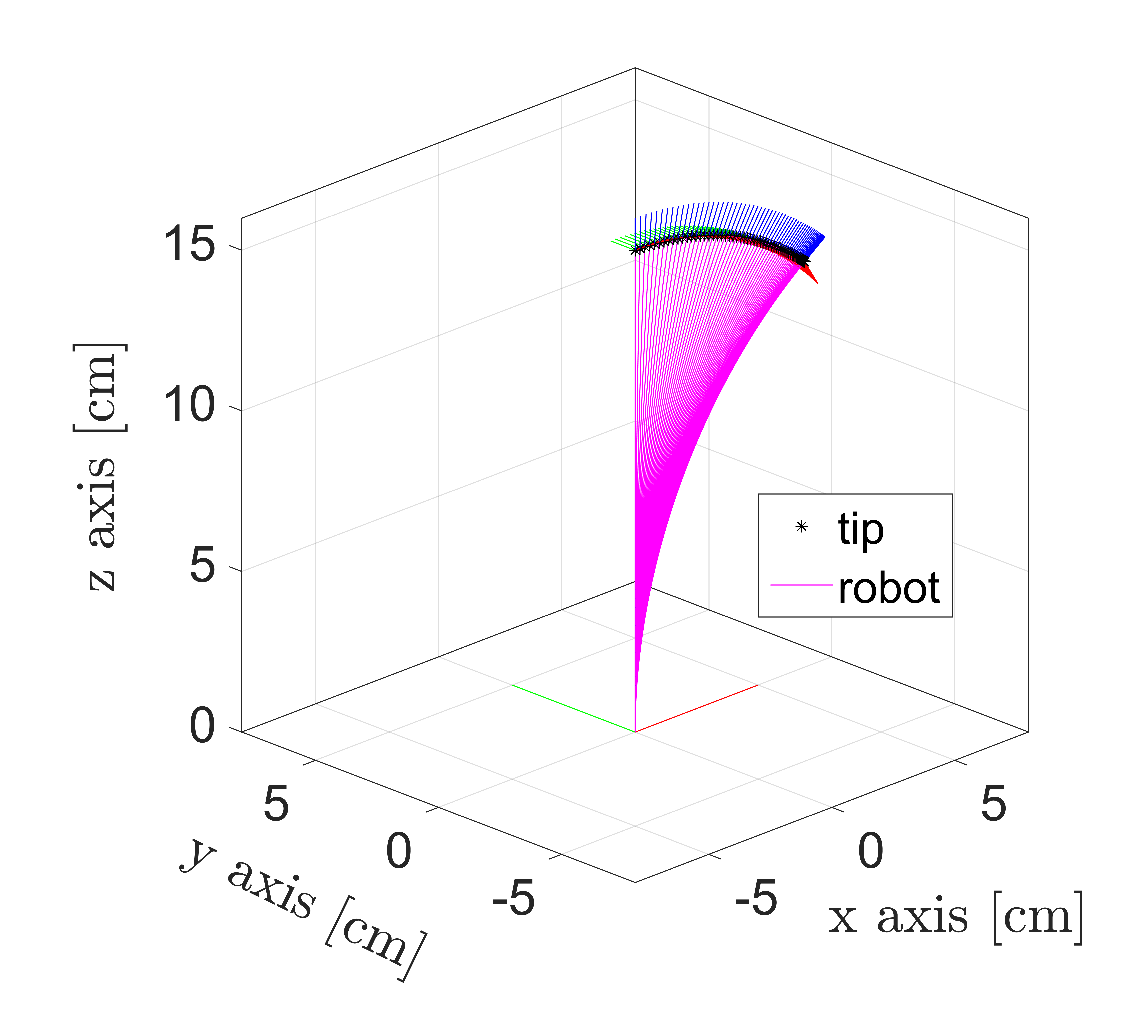
\includegraphics[width=0.21\textwidth]{srslam/figures/t1_l15_v3.0.eps}\label{fig:srslam:traj1}}
  \hspace{0.005\textwidth}% \hfill% or \hspace{5mm} or \hspace{0.3\textwidth}
  \subfigure[Trajectory 2]{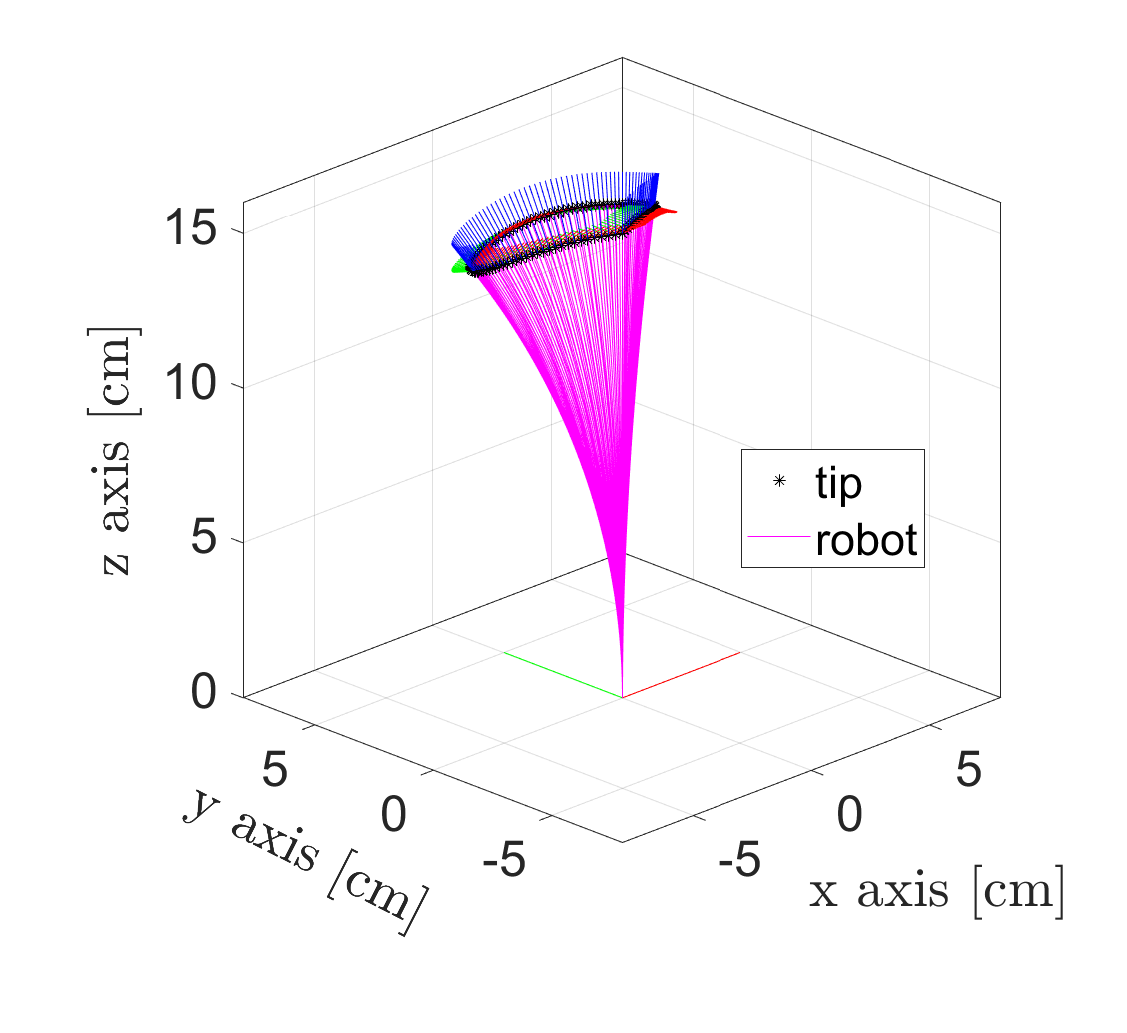
\includegraphics[width=0.21\textwidth]{srslam/figures/t2_l15_v3.2.eps}\label{fig:srslam:traj2}}\hspace{0.005\textwidth}% \hfill% or \hspace{5mm} or \hspace{0.3\textwidth}
  \subfigure[Trajectory 3]{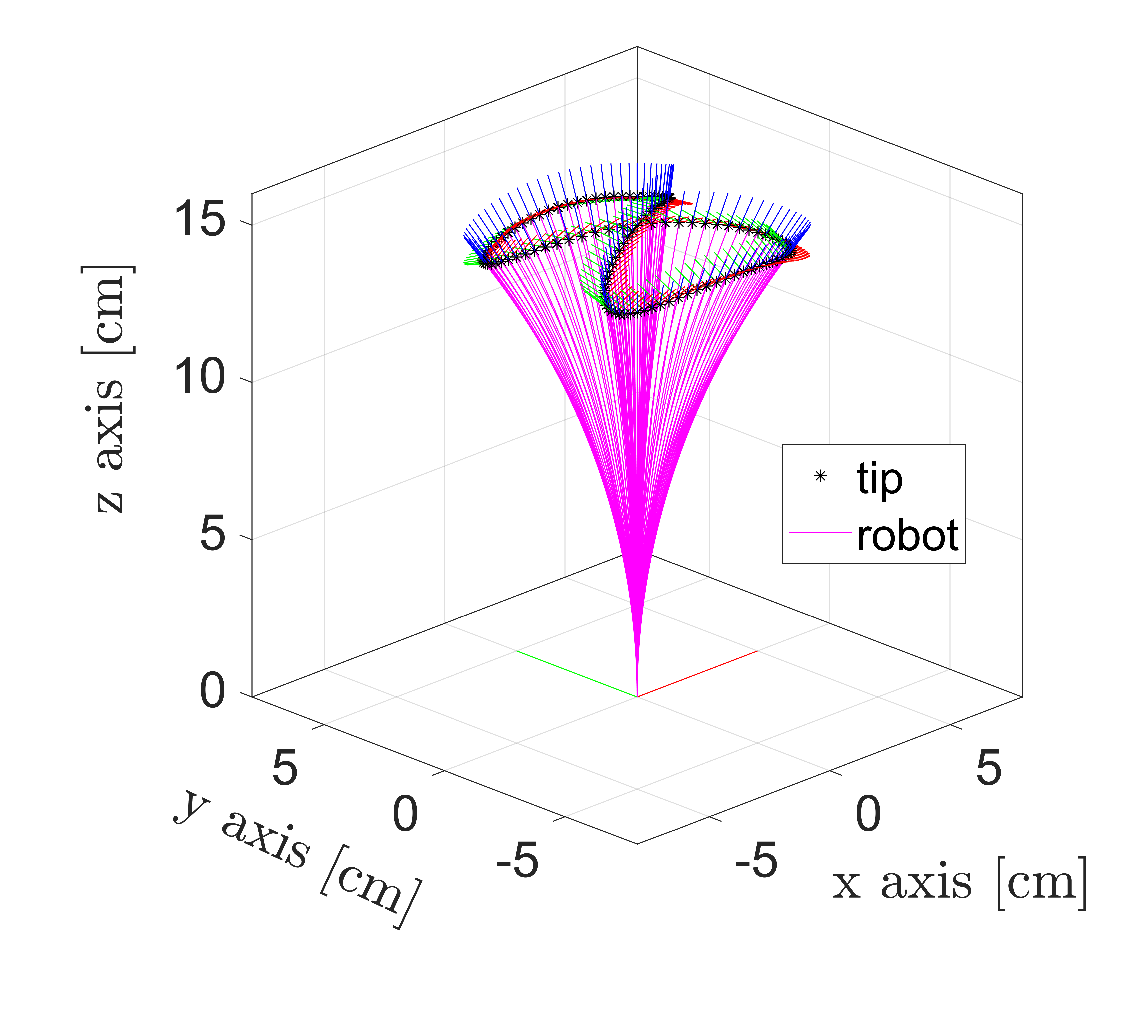
\includegraphics[width=0.21\textwidth]{srslam/figures/t3_l15_v3.1.eps}\label{fig:srslam:traj3}}\hfill
  \subfigure[Virtual interior scene]{\includegraphics[width=0.3\textwidth]{srslam/figures/interior_scene.pdf}\label{fig:srslam:interior_scene}}
  \caption{3D visualization of the three trajectories used in our simulations and experiments for a segment with \SI{15}{cm} length. In magenta, we visualize the trajectory of the full robot, and in black, the tip positions. Additionally, the tip orientation (red = x-axis, green = y-axis, blue = z-axis) is displayed. The virtual interior scene used for the Blender renderings is presented in the last column.}
  \label{fig:srslam:trajectories}
\end{figure*}

In addition to the robot trajectory, a calibration sequence trajectory is designed to initialize the \gls{SLAM} map. 
It is good practice to move the camera parallel to the scene captured. Accordingly, we decide to move the camera into the $x$ cardinal direction of the segment base frame with the translation distance proportional to the robot length.

\subsection{Rendering of Synthetic Images}
The rendering software Blender allows us, among other things, to load a 3D model of the environment, follow customized trajectories with a virtual camera, and render photo-realistic synthetic pictures of the environment from the chosen camera perspective. We use an interior scene published by \href{https://www.nextwavemultimedia.com/html/3dblendermodel.html}{Nextwave Multimedia}. We report a view of the scene in Fig. \ref{fig:srslam:interior_scene}.
The virtual camera is set to be perspective with a focal length of \SI{30}{mm}.
For each run, we randomly initialize the trajectory at one of seven predefined launch points in the indoor environment to diversify the coverage of the environment.
The x-, y-, and z-coordinates of the seven initial positions have a standard deviation of \SI{0.5}{m}, \SI{0.2}{m}, \SI{0.4}{m} respectively. The initial orientation represented in XYZ Euler angles varies with a standard deviation of \SI{0.05}{rad}, \SI{0.13}{rad}, and \SI{1.17}{rad}.
For each trajectory, we render $120$ synthetic images along the trajectory and save them to a folder for later offline processing by the ORB-SLAM~\citep{mur2017orb} algorithm. Fig. \ref{fig:srslam:sequences_of_stills_simulations_cropped} reports a few representative stills of what the robot sees during one execution of the three trajectories discussed above.

\begin{figure*}
    \centering
    \includegraphics[width=0.9\textwidth]{srslam/figures/graphic_sequences_of_stills_simulations_compressed.pdf}
    \caption{Sequence of stills showing the rendered images by the virtual camera in Blender for three different trajectories and a robot segment of length \SI{15}{cm}. The trajectories are visualized in Figure~\ref{fig:srslam:trajectories}.}
    \label{fig:srslam:sequences_of_stills_simulations_cropped}
\end{figure*}

\subsection{Implementation of ORB-SLAM}
The synthetic images along the trajectory are processed offline by the ORB-SLAM~\citep{mur2017orb} algorithm. We rely on the official MATLAB implementation of ORB-SLAM. While we run our simulations offline to decouple any delays by the rendering and/or \gls{SLAM} pipeline, we would like to point out that other ORB-SLAM implementations, such as, for example, in C++, are able to be run in real-time at frame rates of between \SI{10}{Hz} to \SI{30}{Hz}~\citep{mur2017orb}.

\subsection{Projection into PCC kinematics}
The trade-off parameter $\lambda_\mathrm{R}$ between the rotational and the translational error in the cost function \eqref{eq:srslam:cost_fun} was manually tuned and set to $\lambda_\mathrm{R}=0.4$.
As the simulations do not contain any elongations of the segment, we set $\delta L_1 = 0$ in \eqref{eq:srslam:transformation_improved_pcc}. 
We solve the optimization problem outlined in \eqref{eq:srslam:cost_fun} using nonlinear least-squares with the Levenberg-Marquardt solver~\citep{levenberg1944method, marquardt1963algorithm} implemented in MATLAB as \emph{lsqnonlin}.

\subsection{Evaluation metrics}
To quantitatively evaluate the performance of our proposed approach, we introduce error metrics for both the translation and orientation estimates.
%
We measure the translational pose prediction error with a relative \gls{RMSE} $e_\mathrm{t}$
\begin{equation}\label{eq:srslam:evaluation_translational_error}
    e_\mathrm{t} = \frac{\sqrt{\sum_{t=1}^{n_\mathrm{t}} \left (\lVert \hat{t}_{0,t}^{\mathrm{c},1} - t_{0,t}^{\mathrm{c},1} \rVert_2 \right )^2}}{\sqrt{n_\mathrm{t}} \; l_\mathrm{traj}},
\end{equation}
where $l_\mathrm{traj}$ corresponds to the length of the trajectory and $n_\mathrm{t}$ the total number of data points along the trajectory. Similarly, we leverage the Frobenius norm for the rotational error $e_\mathrm{R}$
\begin{equation}\label{eq:srslam:evaluation_rotational_error}
    e_\mathrm{R} = \sqrt{\sum_{t=1}^{n_\mathrm{t}} \frac{\left (\big\lVert \hat{R}_{0,t}^{\mathrm{c},1} - R_{0,t}^{\mathrm{c},1} \big\rVert_F \right )^2}{n_\mathrm{t}}}.
\end{equation}
As torsion can often be neglected for soft robotic arms, we state the angle error for the orientation of the local z-axis of the tip of the segment for intuitive analysis of the orientation estimates. First, the unit vector of the local z-axis $\{ o_{1} \}_{0}$ is computed in the base frame $\{ S_0 \}$
\begin{equation}
    \{ o_1 \}_0 = R_{0,t}^{1}\begin{pmatrix}0 & 0 & 1\end{pmatrix}^\top,
    \quad
    \{ \hat{o}_1 \}_0 = \hat{R}_{0,t}^{1}\begin{pmatrix}0 & 0 & 1\end{pmatrix}^\top,
\end{equation}
which allows us to subsequently compute the angle error between the ground-truth z-axis of the tip $\{ o_1 \}_0$ and the estimated z-axis $ \{ \hat{o}_1 \}_0$
\begin{equation}\label{eq:srslam:evaluation_angle_error}
    e_{\theta_z} = \sqrt{\sum_{t=1}^{n_\mathrm{t}} \frac{\left (\arccos \left ( \{ o_1 \}_0 \cdot \{ \hat{o}_1 \}_0 \right ) \right )^2}{n_\mathrm{t}}}.
\end{equation}

\subsection{Results}\label{sub:srslam:simulation_results}
% \begingroup
% \setlength{\tabcolsep}{2.0pt} % Default value: 6pt
% \renewcommand{\arraystretch}{1} % Default value: 1
\begin{table*}
\centering
\caption{Relative \gls{RMSE} [\%] for translations as referenced in \eqref{eq:srslam:evaluation_translational_error} of various trajectories and of robot segments with different lengths (\SI{15}{cm}, \SI{30}{cm}, \SI{100}{cm}). We state the error as $\text{mean} \pm \text{stdev} \; (\min, \max)$ and compute the statistics over seven trials from different initial poses.}
\begin{tabular}{cclll}\toprule
\textbf{Trajectory} & \textbf{Optimization} & $L_{0,1} = \SI{15}{cm}$ & $L_{0,1} = \SI{30}{cm}$ & $L_{0,1} = \SI{100}{cm}$\\
\midrule
Trajectory 1 & No & $9 \pm 3 \; (5, 12)$ & $7 \pm 3 \; (3, 13)$ & $3 \pm 2 \; (1, 7)$ \\
Trajectory 1 & Yes & $0.4 \pm 0.2 \; (0.3, 0.8)$ & $2 \pm 1 \; (0, 4)$ & $1.0 \pm 0.7 \; (0.5, 2.3)$ \\
\midrule
Trajectory 2 & No & $9 \pm 4 \; (4, 17)$ & $6 \pm 2 \; (3, 8)$ & $1.9 \pm 0.9 \; (1.0, 3.0)$ \\
Trajectory 2 & Yes & $0.7 \pm 0.7 \; (0.3, 1.8)$ & $0.7 \pm 0.4 \; (0.2, 1.2)$ & $0.6 \pm 0.3 \; (0.3, 0.9)$ \\
\midrule
Trajectory 3 & No & $6 \pm 5 \; (3, 16)$ & $2.6 \pm 0.6 \; (1.7, 3.3)$ & $6 \pm 14 \; (1, 37)$ \\
Trajectory 3 & Yes & $2 \pm 3 \; (0, 9)$ & $0.5 \pm 0.3 \; (0.1, 0.8)$ & $2 \pm 5 \; (0, 15)$ \\
\bottomrule
\end{tabular}
\label{tab:srslam:results_simulations_translation}
\end{table*}
% \endgroup

\iffalse
\begin{table*}
\centering
\caption{Absolute \gls{RMSE} [-] for rotations computed with the Frobenius norm between rotation matrices of various trajectories and of robots with various lengths as referenced in \eqref{eq:srslam:evaluation_rotational_error}. We state the error as $\text{mean} \pm \text{stdev} \; (\min, \max)$ and compute the statistics over seven trials from different initial poses.}
\begin{tabular}{cclll}\toprule
\textbf{Trajectory} & \textbf{Optimization} & $L_{0,1} = \SI{15}{cm}$ & $L_{0,1} = \SI{30}{cm}$ & $L_{0,1} = \SI{100}{cm}$\\
\midrule
    Trajectory 1 & No & $0.010 \pm 0.004 \; (0.003, 0.015)$ & $0.016 \pm 0.007 \; (0.008, 0.027)$ & $0.027 \pm 0.017 \; (0.010, 0.051)$ \\
    Trajectory 1 & Yes & $0.007 \pm 0.002 \; (0.003, 0.010)$ & $0.012 \pm 0.007 \; (0.004, 0.023)$ & $0.027 \pm 0.019 \; (0.013, 0.062)$ \\
    \midrule
    Trajectory 2 & No & $0.02 \pm 0.02 \; (0.01, 0.05)$ & $0.011 \pm 0.006 \; (0.005, 0.022)$ & $0.015 \pm 0.008 \; (0.006, 0.025)$ \\
    Trajectory 2 & Yes & $0.02 \pm 0.02 \; (0.00, 0.06)$ & $0.016 \pm 0.009 \; (0.003, 0.025)$ & $0.019 \pm 0.008 \; (0.009, 0.030)$ \\
    \midrule
    Trajectory 3 & No & $0.1 \pm 0.2 \; (0.0, 0.4)$ & $0.010 \pm 0.002 \; (0.006, 0.012)$ & $0.2 \pm 0.4 \; (0.0, 1.1)$ \\
    Trajectory 3 & Yes & $0.1 \pm 0.2 \; (0.0, 0.4)$ & $0.02 \pm 0.01 \; (0.00, 0.034)$ & $0.2 \pm 0.3 \; (0.0, 0.9)$ \\
\bottomrule
\end{tabular}
\label{tab:srslam:results_simulations_rotation_frobenius}
\end{table*}

\begin{table*}
\centering
\caption{Absolute \gls{RMSE} [rad] for rotations computed with dot product \textcolor{red}{...}. We state the error as $\text{mean} \pm \text{stdev} \; (\min, \max)$ and compute the statistics over seven trials from different initial poses.}
\begin{tabular}{cclll}\toprule
\textbf{Trajectory} & \textbf{Optimization} & $L_{0,1} = \SI{15}{cm}$ & $L_{0,1} = \SI{30}{cm}$ & $L_{0,1} = \SI{100}{cm}$\\
\midrule
    Trajectory 1 & No & $0.005 \pm 0.002 \; (0.002, 0.007)$ & $0.009 \pm 0.005 \; (0.004, 0.018)$ & $0.02 \pm 0.01 \; (0.01, 0.04)$ \\
    Trajectory 1 & Yes & $0.005 \pm 0.002 \; (0.002, 0.006)$ & $0.008 \pm 0.005 \; (0.003, 0.016)$ & $0.02 \pm 0.01 \; (0.01, 0.04)$ \\
    \midrule
    Trajectory 2 & No & $0.02 \pm 0.02 \; (0.00, 0.04)$ & $0.006 \pm 0.002 \; (0.003, 0.010)$ & $0.009 \pm 0.005 \; (0.003, 0.016)$ \\
    Trajectory 2 & Yes & $0.01 \pm 0.02 \; (0.00, 0.04)$ & $0.005 \pm 0.002 \; (0.002, 0.009)$ & $0.013 \pm 0.006 \; (0.006, 0.020)$ \\
    \midrule
    Trajectory 3 & No & $0.1 \pm 0.1 \; (0.0, 0.3)$ & $0.006 \pm 0.001 \; (0.004, 0.007)$ & $0.1 \pm 0.2 \; (0.0, 0.4)$ \\
    Trajectory 3 & Yes & $0.1 \pm 0.1 \; (0.0, 0.3)$ & $0.005 \pm 0.002 \; (0.002, 0.008)$ & $0.1 \pm 0.2 \; (0.0, 0.7)$ \\
\bottomrule
\end{tabular}
\label{tab:srslam:results_simulations_rotation_z_angle}
\end{table*}
\fi

\begin{table*}\scriptsize
\centering
\caption{Rotational errors of various trajectories and for robot segments with different lengths (\SI{15}{cm}, \SI{30}{cm}, \SI{100}{cm}). We report both an absolute \gls{RMSE} computed with the Frobenius norm between the rotation matrices as stated in \eqref{eq:srslam:evaluation_rotational_error} and an angle error [rad] for the orientation of the z-axis of the tip of the segment as defined in \eqref{eq:srslam:evaluation_angle_error}. We state the error as $\text{mean} \pm \text{stdev}$ and compute the statistics over seven trials from different initial poses.}
\begin{tabular}{cc cc cc cc}
\toprule
    \multirow{2}{*}{\textbf{Trajectory}} & \multirow{2}{*}{\textbf{Optim.}} & \multicolumn{2}{c}{$L_{0,1} = \SI{15}{cm}$} & \multicolumn{2}{c}{$L_{0,1} = \SI{30}{cm}$} & \multicolumn{2}{c}{$L_{0,1} = \SI{100}{cm}$}\\
    & & $e_\mathrm{R}$ & $e_{\theta_z}$ [rad] & $e_\mathrm{R}$ & $e_{\theta_z}$ [rad] & $e_\mathrm{R}$ & $e_{\theta_z}$ [rad]\\
\midrule
    Trajectory 1 & No & $0.010 \pm 0.004$ & $0.005 \pm 0.002$ & $0.016 \pm 0.007$ & $0.009 \pm 0.005$ & $0.027 \pm 0.017$ & $0.02 \pm 0.01$ \\
    Trajectory 1 & Yes & $0.007 \pm 0.002$ & $0.005 \pm 0.002$ & $0.012 \pm 0.007$ & $0.008 \pm 0.005$ & $0.027 \pm 0.019$ & $0.02 \pm 0.01$ \\
    \midrule
    Trajectory 2 & No & $0.02 \pm 0.02$ & $0.01 \pm 0.02$ & $0.011 \pm 0.006$ & $0.006 \pm 0.002$ & $0.015 \pm 0.008$ &  $0.009 \pm 0.005$ \\
    Trajectory 2 & Yes & $0.02 \pm 0.02$ & $0.01 \pm 0.02$ & $0.016 \pm 0.009$ & $0.005 \pm 0.002$ & $0.019 \pm 0.008$ & $0.013 \pm 0.006$\\
    \midrule
    Trajectory 3 & No & $0.1 \pm 0.2$ &  $0.1 \pm 0.1$ & $0.010 \pm 0.002$ & $0.006 \pm 0.001$ & $0.2 \pm 0.4$ & $0.1 \pm 0.2$\\
    Trajectory 3 & Yes & $0.1 \pm 0.2$ & $0.1 \pm 0.1$ & $0.02 \pm 0.01$ & $0.005 \pm 0.002$ & $0.2 \pm 0.3$ & $0.1 \pm 0.2$\\
\bottomrule
\end{tabular}
\label{tab:srslam:results_simulations_rotation}
\end{table*}

We evaluate our proposed method in simulation on three different robot segment lengths (\SI{15}{cm}, \SI{30}{cm}, and \SI{100}{cm}) and for the three trajectories previously described. 
We state statistical results such as mean, standard deviation, and lower and upper bounds over seven separate trials, each covering a different part of the indoor environment. 
The errors are reported both for the \gls{SLAM} estimates \emph{before} optimization and \emph{after} projection into the \gls{PCC} kinematics.
While the results for the relative \gls{RMSE} of translation estimates through the entire trajectory are shown in Table~\ref{tab:srslam:results_simulations_translation}, the absolute \gls{RMSE} of rotation matrices computed with the Frobenius norm of the rotation matrices or the z-axis orientation axis angle error are displayed in Table~\ref{tab:srslam:results_simulations_rotation}.

Our results show translation errors of in average \SI{6}{\percent} to \SI{9}{\percent} for short segments and \SI{2}{\percent} to \SI{6}{\percent} \gls{RMSE} relative to the trajectory length for long segments before optimization. 
The projection into \gls{PCC} kinematics significantly decreases the translational error by between \SI{66}{\percent} and \SI{96}{\percent} to \SI{0.4}{\percent} to \SI{2}{\percent} for short segments and \SI{0.6}{\percent} to \SI{2}{\percent} for long segments.
%
We state an absolute \gls{RMSE} for the orientation estimates of the z-axis of the tip $e_{\theta_z}$ as defined in Eq.~\ref{eq:srslam:evaluation_angle_error} of between \SI{0.005}{\radian} and \SI{0.1}{\radian} after optimization.
The rotational error of the orientation estimates varies by trial but, on average, stays constant across the optimization. 
Choosing a bigger weight $\lambda_\mathrm{R}$ on the rotational loss during the optimization resulted in larger improvements for estimation of the orientation at the cost of higher translational errors.
\section{Experiments} \label{sec:srslam:experiments}
We confirm the simulation results in a preliminary experimental study by mounting a Raspberry Pi camera to the tip of a soft segment~\cite{katzschmann2019dynamic}. The robotic segment is guided to follow three trajectories similar to the ones tested in simulation (see Section~\ref{sub:srslam:trajectories}). % in 3D space by pneumatically actuating its segment with a pressure regulator. 
A motion capture setup is employed to gather an accurate ground-truth on the shape of the segment.

\begin{figure*}
     \centering
     \subfigure[Experimental setup]{\includegraphics[height=.525\columnwidth]{srslam/figures/graphic_experimental_setup.drawio_v1_compressed.pdf} \label{fig:srslam:experimental_setup}}
     \subfigure[Trajectory 3]{\includegraphics[height=.525\columnwidth]{srslam/figures/graphic_sequences_of_stills_lab_experiment_trajectory_3_compressed.pdf} \label{fig:srslam:graphic_sequences_of_stills_lab_experiment_trajectory_3}}
     \caption{\small In Panel (a), a soft robotic segment is mounted to a cage with attached motion capture cameras. The segment is pneumatically actuated by a pressure regulator (Fest Motion Terminal). A Raspberry Pi camera v2.0 is attached to the tip of the segment and in a straight segment configuration looks down towards check-board patterns. Panel (b) depicts a sequence of stills showing the robot following trajectory 3 from two different vantage points. The second vantage point differs \SI{90}{\degree} from the first one. The third row displays a few representative frames as recorded by the camera attached to the tip of the segment.}
\end{figure*}

\subsection{Experimental setup}
% Segment and manufacturing
We show the experimental setup in Figure~\ref{fig:srslam:experimental_setup}.
We consider a soft robotic silicone segment consisting of four independently inflatable cavities. The segment has a cylindrical shape with a length $L_{0,1}$ of \SI{11}{cm} and a radius $d_1$ of \SI{21}{mm}. 
% We follow the fabrication procedure by Marchese et al.~\cite{marchese2015recipe} by casting Silicone into 3D-printed molds and block any silicon-flow into the air chambers with bees wax.
A 3D-printed ring with four motion capture markers is located near the tip of the segment.
%
% Camera and its attachment to the segment
We mount a Raspberry Pi camera module v2.0 to the tip of the segment.
This camera has a \SI{8}{MP} sensor and records frames at a sampling rate of \SI{30}{Hz} and a resolution of 1080p.
The focal length is \SI{3.04}{mm} and the field of view is $\SI{62.2}{\degree} \times \SI{48.8}{\degree}$.
The camera module is attached to a Raspberry Pi 3B+ single-board computer which saves the frames for later processing by the ORB-SLAM~\cite{mur2017orb} algorithm.
The camera is screwed onto a custom 3D-printed holder which in turn is glued with the tip plane of the segment.
%
% Actuation motion terminal, communication, commanding of pressures
The segment with its four air chambers is actuated with a proportional pressure regulator.
Tubing attached to the base of the segment connects each chamber with the assigned pneumatic valve of the pressure regulator.
%
% We apply a constant offset pressure $p_0$ to all chambers in straight configuration and subsequently synchronously increase the pressure $p_1$ in one chamber by $f_{\mathrm{p},x}$ and decrease the pressure in the opposite chamber $p_2$ by $f_{\mathrm{p},x}$ accordingly to cause a bending of the segment, in this case in x-direction.
% \begin{equation}
% \begin{split}
%     p_1 = p_0 - f_{\mathrm{p},x} \qquad p_2 = p_0 + f_{\mathrm{p},x}\\
%     p_3 = p_0 - f_{\mathrm{p},y} \qquad p_4 = p_0 + f_{\mathrm{p},y}
% \end{split}
% \end{equation}
% We map the desired configuration $\Delta_{x,1}$ and $\Delta_{y,1}$ given by the trajectories defined in \eqref{eq:srslam:trajectory_parametrization} in linear approximation to the commanded pressures
% \begin{equation}
%     f_{\mathrm{p},x} = a_x \; \Delta_{x,1} 
%     \qquad
%     f_{\mathrm{p},y} = a_y \; \Delta_{y,1}
%     \qquad
%     p_0 = a_{\delta L} \; \delta L_1
% \end{equation}
% where the proportional factors $a_{x}$, $a_{y}$ and $a_{\delta L}$ are experimentally determined and an elongation of the segment is reached through an increase in the offset pressure $p_0$.
% The pressure in each chamber is regulated by a Festo Motion Terminal using a factory-tuned PID controller.
% The commanded valve pressures are relayed via Modbus / TCP from our lab workstation to the Motion Terminal at a frequency of approximately \SI{10}{Hz}.
%
% Cage and environment
The segment is attached in up-side-down configuration to the top plane of a cubical cage of \SI{750}{mm} side length. For a straight segment, the camera is facing downwards towards the floor of the cage, which is covered by multiple printed checkerboard patterns.
%
% Motion capture system and cage
We acquire ground-truth pose information of the tip of the segment using an Optitrack motion capture system. %, consisting of eight PrimeX 13 cameras mounted to the previously mentioned cubic cage. 
The ground-truth poses of the tip of the segment are recorded at \SI{30}{Hz}. % analogous to the Raspberry Pi camera frames.
% Additionally, we also record the pose of the base of the segment allowing us to determine a ground-truth coordinate transformation $T_{0}^{1}$ from the base to the tip.
%
% Implementation of PCC projection and calibration sequence
%In contrast to the model we used in simulation, the real-world segment experiences an elongation caused by the application of pressure to the chambers. Accordingly, 
%
We also include the elongation of the segment $\delta L_1$ in the cost function \eqref{eq:srslam:cost_fun} of our optimization.
%
% Calibration sequence
To resemble the calibration sequence from simulation for the \gls{SLAM} map, we manually move the robot lateral into the x-coordinate direction before fixing it to the cage for the start of the experiments.

\subsection{Results}
Our experimental results reported in Table~\ref{tab:srslam:results_lab_experiments} and visualized for trajectory 3 in Figure~\ref{fig:srslam:experiments_t3_over_time} show translational relative \gls{RMSE} of between \SI{9}{\percent} and \SI{20}{\percent} for the three trajectories before optimization. 
The orientation of the z-axis of the tip is estimated with a mean error of approximately \SI{0.075}{\radian}.
The translational error is improved to between \SI{5}{\percent} and \SI{9}{\percent} after projection into the \gls{PCC}-kinematics. 
The optimization also slightly improves the rotational \gls{RMSE} by \SI{4}{\percent} to \SI{10}{\percent} relative to naive \gls{SLAM}.

The experimental results of the \gls{SLAM} algorithm are coherent with the simulations as the small segment length (\SI{11}{cm}) used in the experiments increases the translational errors as shown similarly in the simulations for a robot of length \SI{15}{cm}.
Even though the translational error is greatly reduced through optimization, it is still significantly higher than in simulation. Two reasons for this difference could be that a) the segment in simulation was modelled as in-extensible, while the real robot segment is extended via pneumatic pressurization, which introduces additional errors by \gls{SLAM} not accurately estimating the elongation movement and b) the real robot does not perfectly behave according to the \gls{CC} approximation as the simulated robot does.

% \begin{table}\small
% \centering
% \caption{\small \textcolor{orange}{OLD RESULTS: }oReal-world results before and after optimization: the translational errors are stated through a relative \gls{RMSE} and the rotational errors with an absolute \gls{RMSE} taking into account the Frobenius norm of the rotation matrices.}
% \begin{tabular}{lclll}\toprule
% \textbf{Error category} & \textbf{Opt.} & \textbf{Traj. 1} & \textbf{Traj. 2} & \textbf{Traj. 3}\\
% \midrule
% Translation $e_\mathrm{t}$ Eq.~\eqref{eq:srslam:evaluation_translational_error} & No & $\SI{24.8}{\percent}$ & $\SI{21.4}{\percent}$ & $\SI{9.5}{\percent}$ \\
% Translation $e_\mathrm{t}$ Eq.~\eqref{eq:srslam:evaluation_translational_error} & Yes & $\SI{11.4}{\percent}$ & $\SI{13.0}{\percent}$ & $\SI{4.5}{\percent}$ \\
% \midrule
% Rotation $e_\mathrm{R}$ Eq.~\eqref{eq:srslam:evaluation_rotational_error} & No & $0.105$ & $0.131$ & $0.116$ \\
% Rotation $e_\mathrm{R}$ Eq.~\eqref{eq:srslam:evaluation_rotational_error} & Yes & $0.098$ & $0.125$ & $0.112$ \\
% \midrule
% \textcolor{orange}{Rotation $e_{\theta_z}$ Eq.~\eqref{eq:srslam:evaluation_angle_error}} & No & $0.105$ & $0.131$ & $0.116$ \\
% \textcolor{orange}{Rotation $e_{\theta_z}$ Eq.~\eqref{eq:srslam:evaluation_angle_error}} & Yes & $0.098$ & $0.125$ & $0.112$ \\
% \bottomrule
% \end{tabular}
% \label{tab:srslam:results_lab_experiments}
% \end{table}

\begin{table}\small
\centering
\caption{\small Real-world results before and after optimization. The translational errors are stated through a relative \gls{RMSE} as described in \eqref{eq:srslam:evaluation_translational_error}. For rotation, we report both an absolute \gls{RMSE} computed with the Frobenius norm between the rotation matrices as stated in \eqref{eq:srslam:evaluation_rotational_error} and an angle error [rad] for the orientation of the z-axis of the tip of the segment as defined in \eqref{eq:srslam:evaluation_angle_error}. The results are averaged over two trials for each trajectory.}
\begin{tabular}{lclll}\toprule
\textbf{Error category} & \textbf{Opt.} & \textbf{Traj. 1} & \textbf{Traj. 2} & \textbf{Traj. 3}\\
\midrule
Translation $e_\mathrm{t}$ & No & $\SI{20.3}{\percent}$ & $\SI{14.2}{\percent}$ & $\SI{9.1}{\percent}$ \\
Translation $e_\mathrm{t}$ & Yes & $\SI{9.1}{\percent}$ & $\SI{8.9}{\percent}$ & $\SI{5.0}{\percent}$ \\
\midrule
Rotation $e_\mathrm{R}$ & No & $0.145$ & $0.103$ & $0.126$ \\
Rotation $e_\mathrm{R}$ & Yes & $0.130$ & $0.099$ & $0.120$ \\
\midrule
Rotation $e_{\theta_z}$ & No & $\SI{0.079}{\radian}$ & $\SI{0.068}{\radian}$ & $\SI{0.084}{\radian}$ \\
Rotation $e_{\theta_z}$ & Yes & $\SI{0.080}{\radian}$ & $\SI{0.067}{\radian}$ & $\SI{0.084}{\radian}$ \\
\bottomrule
\end{tabular}
\label{tab:srslam:results_lab_experiments}
\end{table}

\begin{figure}[ht]
    \centering
    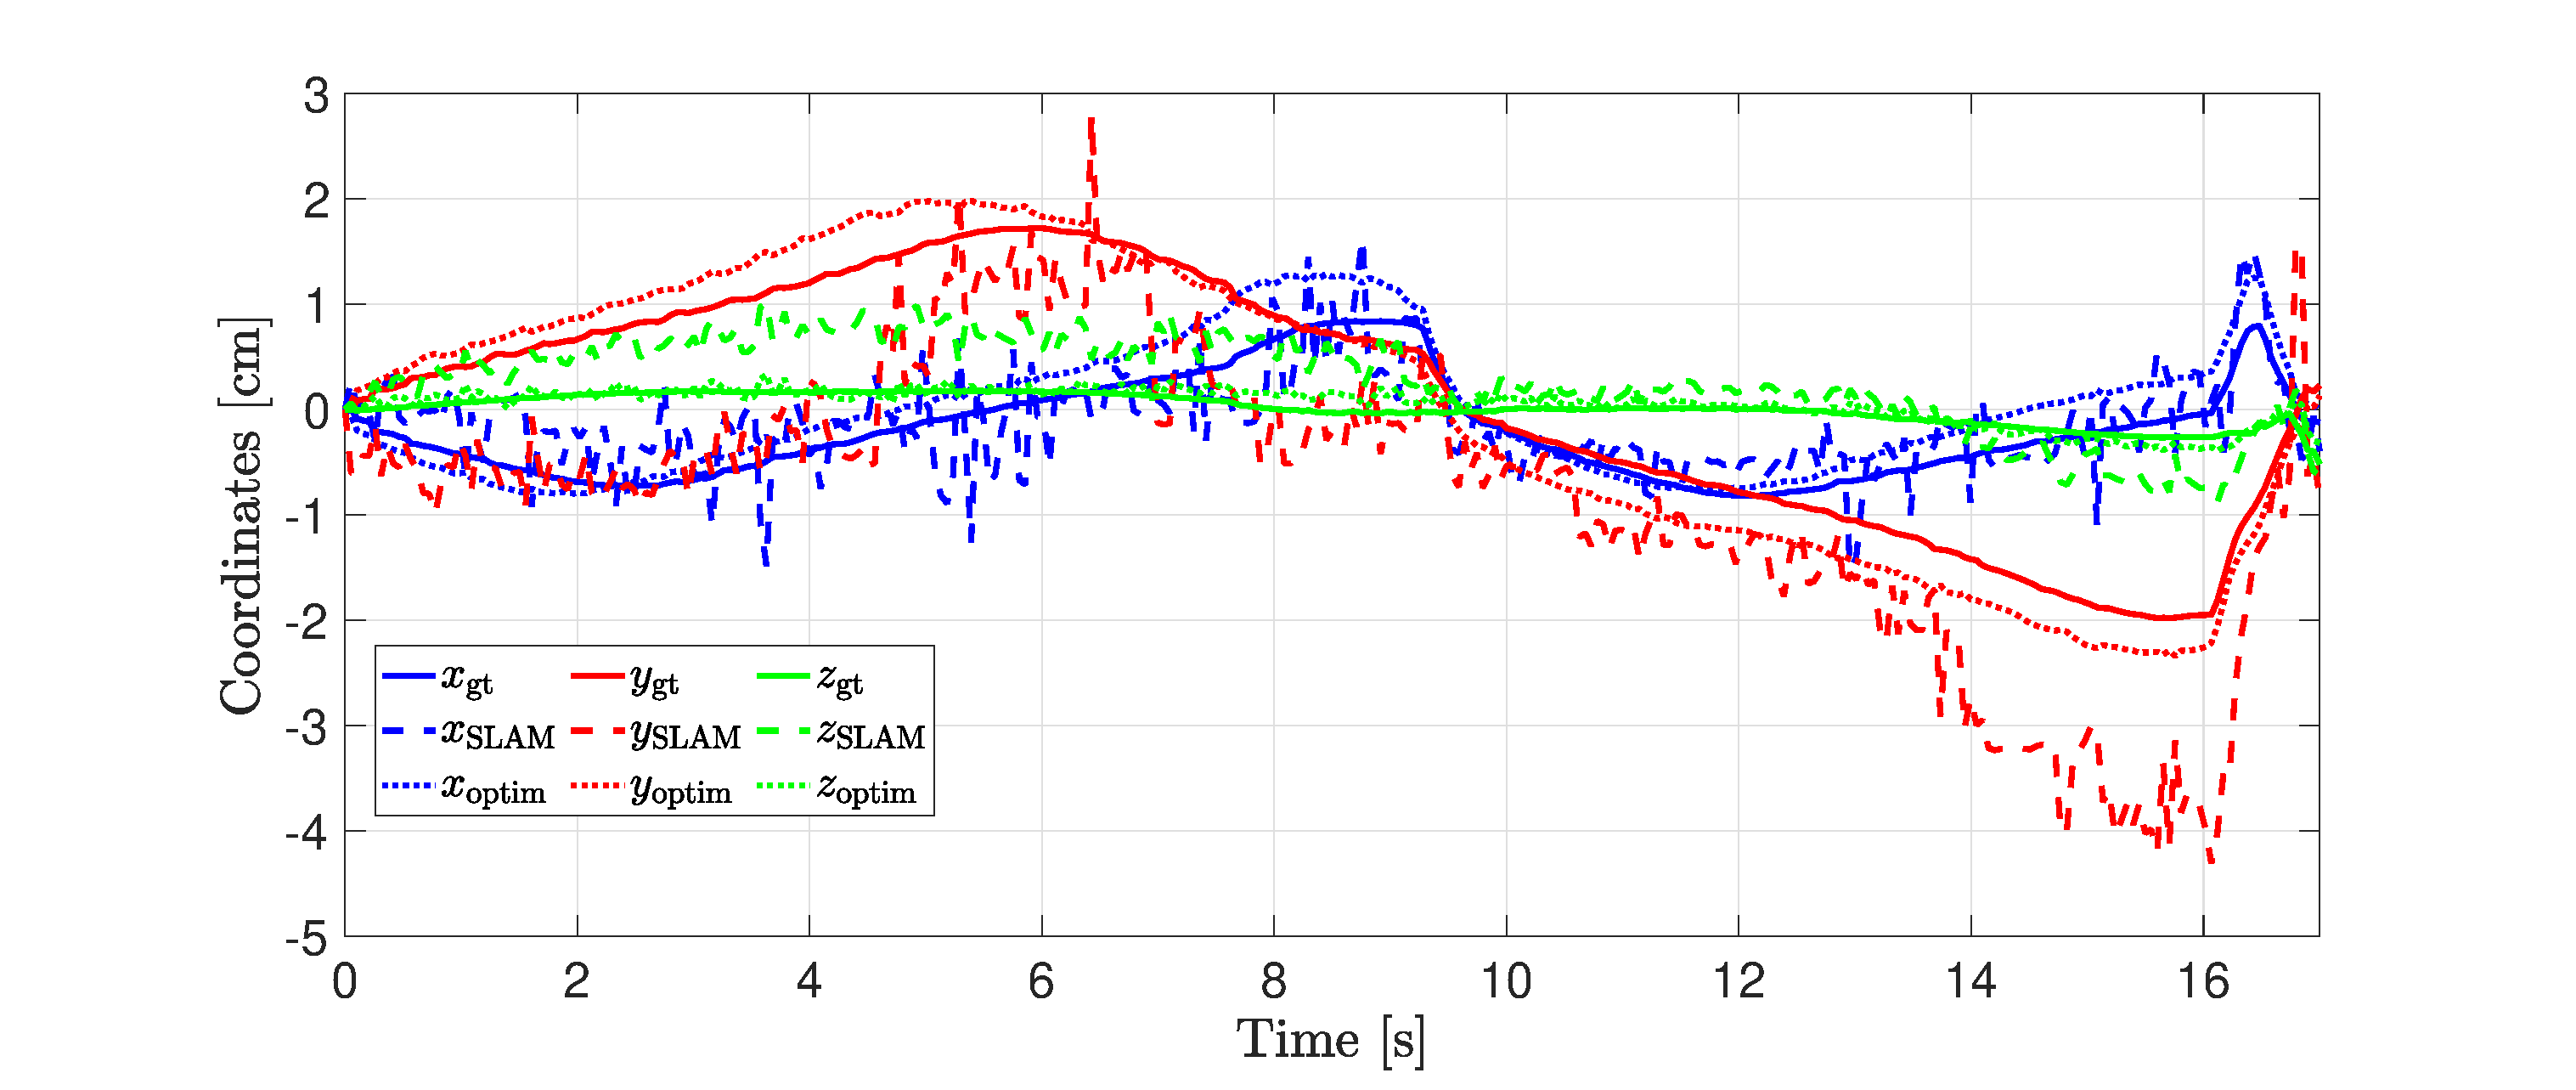
\includegraphics[width=\columnwidth, trim={2cm 1.2cm 2cm 0}]{srslam/figures/vtem28_t3_coordinates.eps}\\
    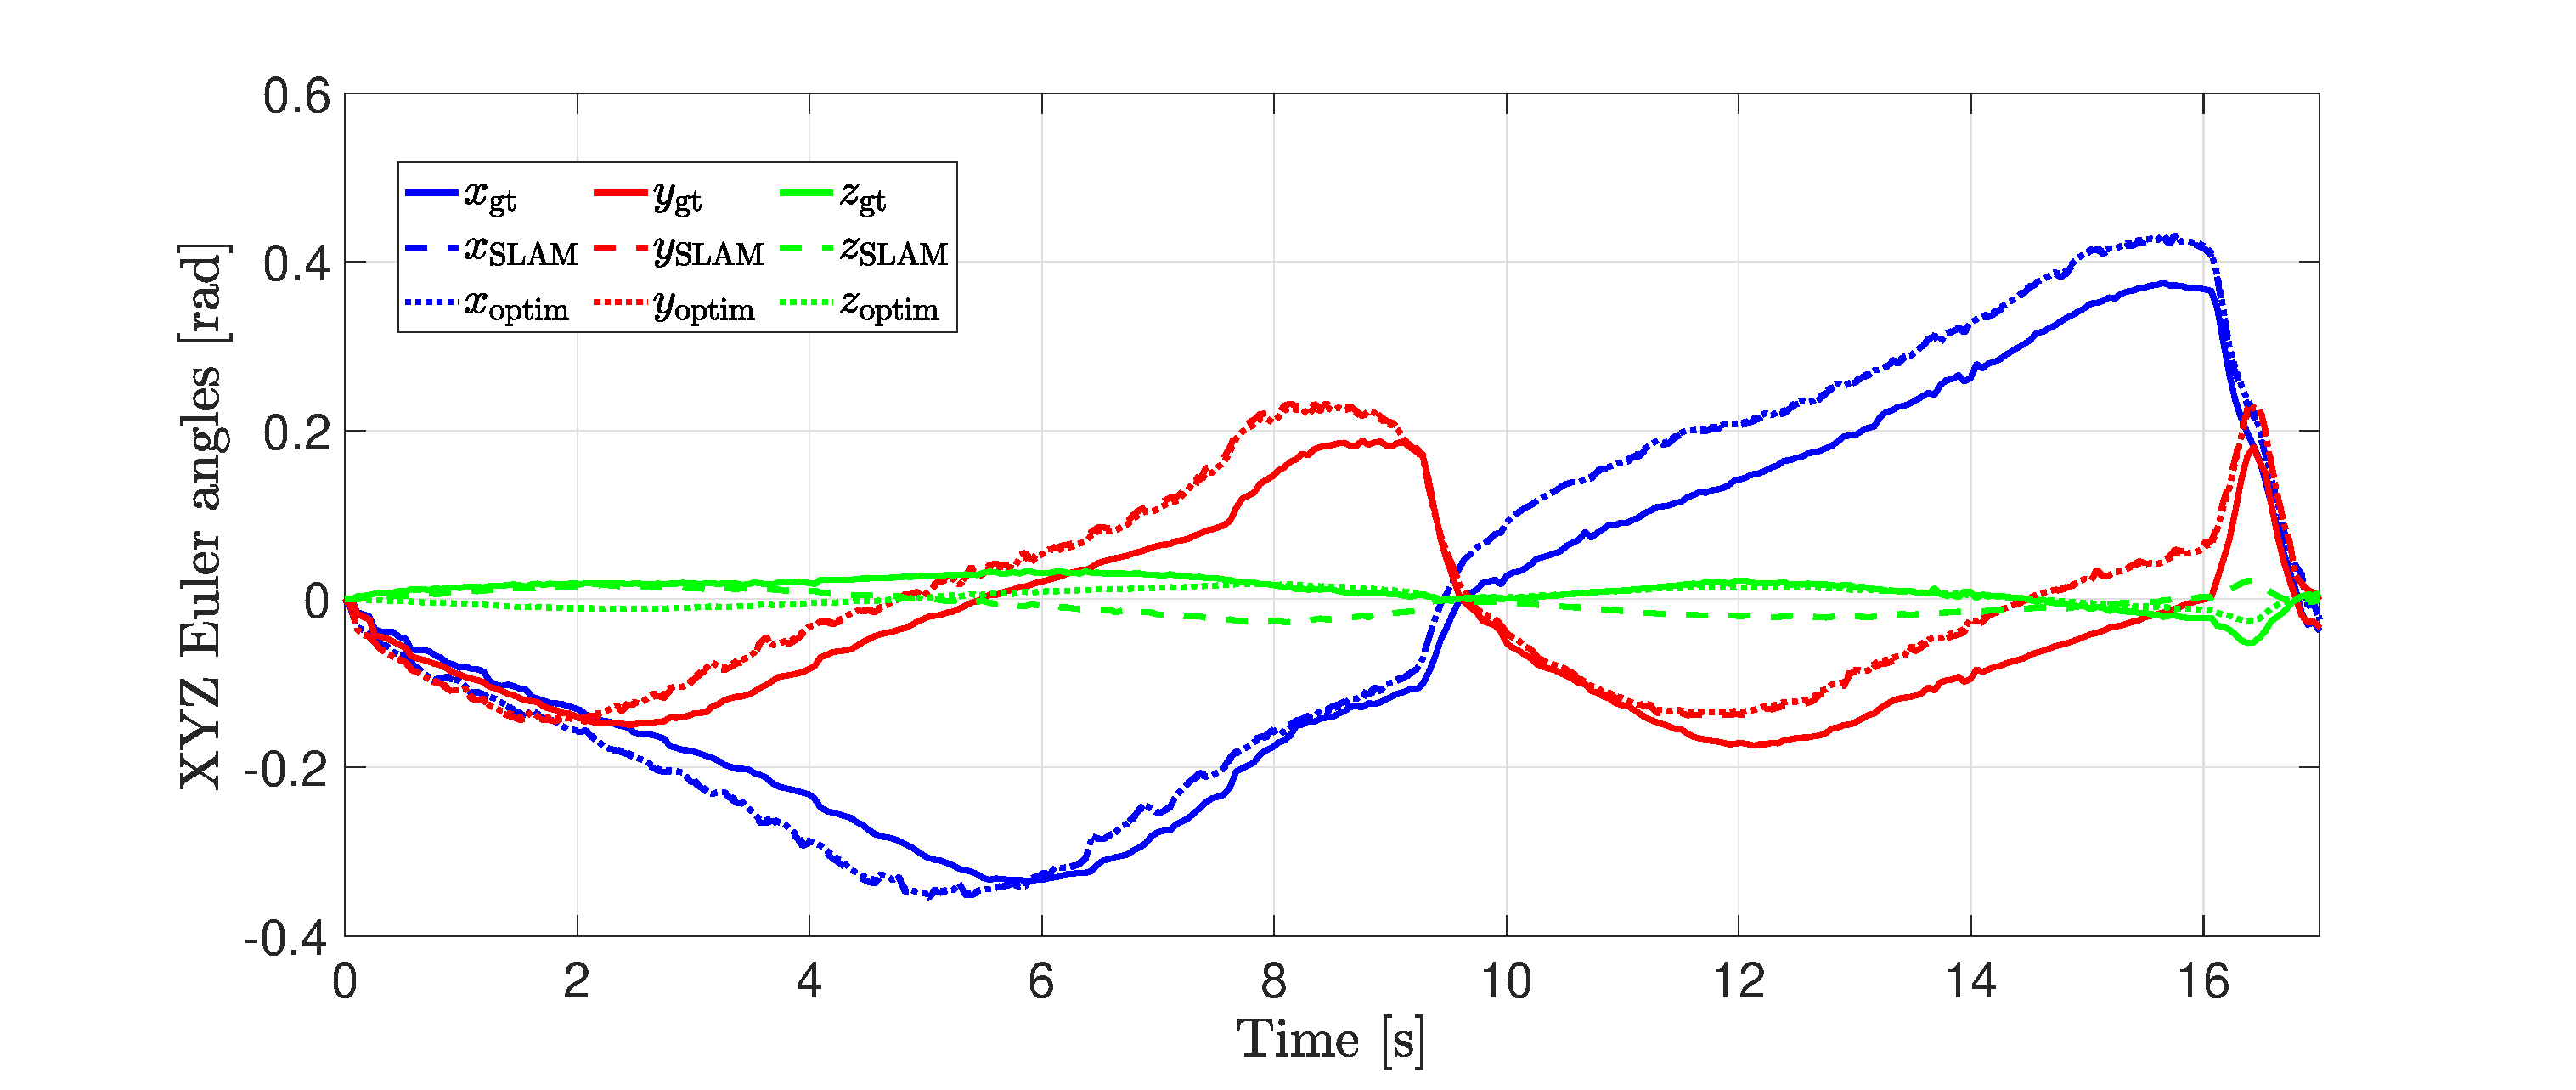
\includegraphics[width=\columnwidth, trim={2cm 0 2cm 1.2cm}]{srslam/figures/vtem28_t3_angles.eps}
    \caption{\small Experimental results for trajectory 3. Comparison between ground-truth (solid line), \gls{SLAM} (dashed line) and optimized through projection into \gls{PCC} kinematics (dotted line) for translation and orientation estimates.}
    \label{fig:srslam:experiments_t3_over_time}
\end{figure}


\section{Conclusion}
\label{sec:srslam:conclusions}

This chapter investigated using a monocular camera in shape sensing of continuum soft robots, with the ultimate goal of implementing precise and reliable estimations at the cost of introducing small rigid parts into the hardware design. The contribution of this chapter has been twofold. First, we proposed to use monocular \gls{SLAM} with a soft robot. Second, we propose a regularization of the estimation based on a nonlinear projection in the manifold of the admitted configuration. A nonlinear optimization implements the latter based on the kinematic model of the robot. We have performed extensive simulations with rendered images in Blender and lab experiments with a single-segment soft robot. The nonlinear optimization based on the robot's kinematic model led to a significant improvement in translations and a marginal improvement in rotations. 
Future work will focus on extending the experimental validation of the method to multiple segments and cameras, bettering the SLAM by feeding back the kinematic projection in its state, and using this estimation to implement closed-loop control.
While we conducted our experiments in a lab environment under ideal conditions with the camera pointed at checkerboard patterns, thus resulting in plenty of image features for \gls{SLAM} to track, future work should investigate whether deployment environments for soft robots would be sufficiently feature-rich for the use of our proposed method.

\section{Afterword}
This chapter demonstrated how inexpensive commercialized monocular cameras can be effectively used together with established \gls{SLAM} algorithms and kinematic models (e.g., \gls{PCC}) to achieve shape sensing for soft robots. One of the main advantages of this solution is that all necessary components are readily available - either commercially or even via open source. However, the presented approach also has some drawbacks: 
i) Firstly, while cameras have been significantly miniaturized in recent years, the requirement for them to have a clear, unobstructed view of the environment necessitates the inclusion of a rigid component on the surface of the soft robot, which we generally prefer to avoid for safety reasons. 
Secondly, ii), the performance of \gls{SLAM} algorithms is affected in environments with limited visually distinguishable features.
Finally, iii) high-dimensional perceptive data such as images are generally computationally expensive to process, leading to higher computational requirements and/or relatively low sampling rates of the shape-sensing information.
Therefore, we present in Chapter~\ref{chp:promasens} an alternative shape-sensing approach based on magnetic sensors. The necessary magnets and magnetic sensors can be deeply embedded into the soft robot body, thus allowing us to keep the robot surface entirely soft and compliant. Furthermore, the sensory data is several orders of magnitude lower dimensional, and thus, its processing is potentially much less computationally demanding.

\chapter{Modelling of Handed Shearing Auxetics (HSA) Robots}
\label{chp:hsamodel}

\begin{abstract}
    Electrically-actuated continuum soft robots based on Handed Shearing Auxetics (HSAs) promise rapid actuation capabilities while preserving structural compliance. However, the foundational models of these novel actuators required for precise control strategies are missing. This paper proposes two key components extending discrete Cosserat rod model (DCM) to allow for modeling HSAs. First, we propose a mechanism for incorporating the auxetic trajectory into DCM dynamical simulations. We also propose an implementation of this extension as a plugin for the Elastica simulator. Second, we introduce a Selective Piecewise Constant Strain (SPCS) kinematic parameterization that can describe an HSA segment's shape with fewer configuration variables. We verify both theoretical contributions experimentally. The simulator is used to replicate experimental data of the mechanical characterization of HSA rods. For the second component, we attach motion capture markers at various points to a parallel HSA robot and find that the shape of the HSAs can be kinematically represented with an average accuracy of \SI{0.3}{mm} for positions and \SI{0.07}{rad} for orientations.
\end{abstract}

\blfootnote{This chapter is partly based on 
\begin{itemize}
    \item[\faFileTextO] ~\emph{\textbf{M. Stölzle}, L. Chin, R. L. Truby, D. Rus, and C. Della Santina (2023, April). Modelling Handed Shearing Auxetics: Selective Piecewise Constant Strain Kinematics and Dynamic Simulation. In 2023 IEEE International Conference on Soft Robotics (RoboSoft) (pp. 1-8). IEEE}~\cite{stolzle2023modelling}.
    \item[\faFileTextO] ~\emph{\textbf{M. Stölzle}, D. Rus, and C. Della Santina (2023, December). An Experimental Study of Model-based Control for Planar Handed Shearing Auxetics Robots. In Experimental Robotics: The 18th International Symposium. Springer}~\cite{stolzle2024experimental}.
\end{itemize}
}


%% Start the actual chapter on a new page.
\newpage

\section{Introduction}\label{sec:hsamodel:introduction}

% Continuum soft robots promise natural compliance and safe interaction with humans, thanks to their invertebrate-inspired bodies~\citep{della2020softencyclopedia}. Several actuation technologies for soft robots have been explored in recent years, with the most popular being cable-driven and pneumatic actuation~\citep{zaidi2021actuation}.
% Although pneumatically-driven soft robots have been successfully used~\citep{falkenhahn2015dynamic, franco2021position, zaidi2021actuation}, their speed is rather slow and their pneumatic actuation cannot generate twisting thus limiting their Degrees of Freedom (DoF) in task space.
% Cable-driven soft robots generate a pulling force with electric motors using a tendon attached to a soft structure, relying on the elasticity of the system to generate a motion.
%While similarly electrically actuated, 

\dropcap{R}obots based on \glsxtrfull{HSA} are a recent development in the soft robotics field~\citep{chin2018compliant, truby2021recipe, zhang2022vision, lipton2018handedness, chin2019automated}, which directly transform applied motor torques into complex motion primitives.
%
This novel type of actuator is based on an architected metamaterial. The most important characteristic of this cylindrical metamaterial is that twist strains along the handedness of the structure lead to an elongation of the rod, which is also called auxetic trajectory~\citep{good2022expanding}. 
% These twist strains can be imposed by electric actuation thus enabling fast system responses~\citep{garg2022kinematic}. 
An \gls{HSA} robot combines multiple \glspl{HSA} of different handedness with a platform constraining the movement of the distal ends in the fashion of a soft parallel manipulator. 
Differential elongation of the rods enables complex motion primitives such as elongation, bending, and twisting~\citep{chin2018compliant}, which can be seen in Fig.~\ref{fig:hsamodel:motion_primitives}. % lipton2018handedness
\gls{HSA} robots are particularly difficult to model and control as the forces and torques causing the evolution of the system are not directly produced by the actuator but instead are intrinsically generated as an effect of the modified cell state of the metamaterial and of the interaction forces coming from the parallel arrangement.

\begin{figure}
    \centering
    \includegraphics[width=0.72\columnwidth]{hsamodel/figures/overview/overview_v2_cropped.pdf}
    \caption{An HSA robot in a twisted state: simulation and schematic of the kinematic model of a single HSA rod.}
    \label{fig:hsamodel:overview}
\end{figure}

%This twist strain can be imposed by constraining the tip and simultaneously actuating the proximal end of the \glspl{HSA} with electric servo motors thus enabling fast system responses~\citep{garg2022kinematic}. Combining multiple rods (usually four) of different handedness with a platform at the distal end creates a \gls{HSA} robot. Differential elongation of the rods and leveraging the torsional torques by the motors enable complex motion primitives such as elongation, bending, and twisting~\citep{chin2018compliant, lipton2018handedness}, which can be seen in Fig.~\ref{fig:hsamodel:motion_primitives}.

% This novel type of soft robot consists of four pillars of architected metamaterials.
% The important characteristic of each of the cylindrical auxetics is that twist strains following the handedness of the pattern cause an elongation of the rod. 
% Each of these \glspl{HSA} is independently actuated using electric servo motors thus enabling fast system responses~\citep{garg2022kinematic}.

% Although the latest advances in 3D-printing of metamaterials via digital projection lithography~\citep{truby2021recipe} have made the manufacturing of \gls{HSA} robots much easier, the technology is still expensive and in its infancy. This lack of accessibility severely limits the progress on modeling the behaviour of \gls{HSA} robots and control them successfully. Therefore, a fast simulator is a necessity to allow the research community to rapidly prototype new control strategies.
3D-\gls{FEM} based approaches~\citep{farrell2020extension} have proven to be effective in simulating soft parallel structures \citep{vanneste2021enabling} and could be a good candidate for representing the complex behavior of \gls{HSA} robots. However, in this chapter, we strive for a less computationally expensive solution - towards applications in model-based control \citep{della2023model}. For this reason, we look at the framework of the \gls{DCM}. The Cosserat rod theory assumes the slenderness of the object, e.g., that the length is much larger than the radius, and allows for the rod to exhibit all six principal strains. The 1D discretization of the rod along its length dramatically reduces the computational demand compared to \gls{FEM}~\citep{gazzola2018forward}. 
% The main modification compared to the SoA simulators~\citep{naughton2021elastica, mathew2022sorosim} is that we couple the twist strains to the rest length of the rod. 
%
Several works in recent literature have successfully applied this framework to soft robotics \citep{grazioso2019geometrically,sadati2021tmtdyn,armanini2023soft}. Among them, in \gls{PCS}~\citep{renda2018discrete}, the continuum dynamics of the Cosserat model are discretized in space by keeping a selection of strains constant along a segment of the continuum. %They all neglect volumetric deformations and focus on the behavior of the central axis~\citep{della2021model}. 
The most popular \gls{PCS} is \gls{PCC}~\citep{webster2010design}, which assumes a sequence of arcs. Functional extensions of \gls{PCS} use a continuous function to approximate the strain~\citep{della2019control,renda2020geometric}. %The functional subspace is split into basis functions and weights, which are taken as the configuration of the robot~\citep{della2021model}. 
% Finally, \gls{FEM} models represent the shape of the continuum with a mesh~\citep{grazioso2019geometrically}, therefore not neglecting the volumetric deformations.

\begin{figure*}[hbt]
    \centering
    \includegraphics[width=1.0\textwidth]{hsamodel/figures/motion_primitives/motion_primitives_v2_compressed.pdf}
    
    \caption{Motion primitives of \gls{HSA} robots: elongation, bending in the four cardinal directions (e.g., north (N), south (S), west (W), east (E)), and clockwise (CW) and counter-clockwise (CCW) twisting.
    \textbf{First row (a):} depicts the necessary actuation inputs to generate these motion primitives. Pure elongation is achieved by applying the motor torques of the same magnitude but in opposite directions to the left-handed (L) and right-handed (R) \glspl{HSA}. For bending, a delta exists in the elongation of the rods, while the sum of torques is still zero. Last but not least, counter-clockwise twisting is achieved by applying more torque to the right-handed than to the left-handed HSA rods.
    \textbf{Second row (b):} Snapshots of the experimental platform when actuated according to the above-specified sequence.
    \textbf{Third row (c):} Renderings of simulated steady-states of an HSA robot. It consists of four HSA rods and a platform at the distal end. The red arrows point along the local x-axis, and the green arrows along the local y-axis, respectively. The blue arrow signifies the z-axis of the local frame of the platform.}\label{fig:hsamodel:motion_primitives}
\end{figure*}

However, none of these methods are currently applicable to HSA robots, as they do not embed a mechanism for incorporating the effect of the auxetic trajectory.
%
We are aware of just one work looking into kinematic modeling of HSA robots~\citep{garg2022kinematic}, which, however, models the backbone of the robot with \gls{PCC} instead of modeling the HSAs. As a consequence, the model cannot represent complex behaviors of the module, like the twist in Fig.~\ref{fig:hsamodel:overview}. 

The goal of this chapter is to provide such a mechanism for the general movement of \gls{HSA} robots in 3D-space, to introduce a strategy for further reducing the dimensionality of the model, to derive a control-oriented model for planar \gls{HSA} robots, and to provide extensive experimental validation for all. 
More specifically, our extension to the \gls{DCM} framework couples the twisting strain of the \gls{HSA} rod to its rest length. %The elastic modulus together with the axial strains will then naturally drive the \gls{HSA} towards this rest length.
Additionally, we allow the rigidity of the rod to be modified as a function of the twist strain. %This is necessary as new work on identifying the mechanical characteristics of \glspl{HSA}~\citep{good2022expanding} has shown that the spring constant increases with the twist strains.
We have implemented this mechanism as a plugin for Elastica~\citep{naughton2021elastica}, which we provide open source\footnote{\url{https://github.com/tud-phi/HSA-PyElastica}}. 
% This results in a compact dynamic model that we test experimentally.
% Several SoA simulators simulators~\citep{naughton2021elastica, mathew2022sorosim} rely on this discretized Cosserat rod theory.

We then use a combination of \gls{CS} and \glspl{PCS}~\citep{renda2018discrete} to describe the shape of \gls{HSA} rods, which we call a \gls{SPCS} model: while some strains, such as twist \& stretch, are mostly constant over the length of the entire \gls{HSA}, other strains, such as bend \& shear, significantly vary and are thus captured in a piecewise parametrization. 
Our results show that a kinematic parametrization with $11$ Degrees of Freedom (DoF) is sufficient to capture the shape of \glspl{HSA}.
Compared to the \gls{DCM} strategy used for simulating \glspl{HSA}, we have, therefore, significantly reduced the DoF of the kinematics.
We provide an open-source implementation of this kinematic model in JAX\footnote{\url{https://github.com/tud-phi/jax-spcs-kinematics}}.
% Furthermore, we propose a Selective Piecewise Constant Strain (SPCS) kinematic model to describe the full 3D deformation of a single \gls{HSA} rod with a dramatically reduced number of states (compared to the \gls{DCM} strategy).

This kinematic model could then be used to parametrize the deformation of each limb in the parallel \gls{HSA} rod.
However, this would require the enforcement of kinematic constraints~\citep {armanini2021discrete}, which can be algorithmically and computationally challenging.
We propose to avoid this complexity in the planar case by natively incorporating the kinematic constraints into the model. In particular, we 
defining the \gls{CS} of a virtual backbone in the center of the robot to be our configuration variable.
Finally, we derive the system dynamics of a planar \gls{HSA} robot in Euler-Lagrangian form.

In summary, we contribute to the state of the art in the modeling of soft robots with:
%
\begin{enumerate}
    \item A mechanism for integrating the auxetic trajectory of \glspl{HSA} into the discrete Cosserat rod theory~\citep{gazzola2018forward, mathew2022sorosim}. %Specifically, we modify the rest length of the rod as a function of the twist strain to cause an elongation of the \gls{HSA}.
    \item A plugin for the Elastica simulator~\citep{naughton2021elastica}, which also includes the necessary boundary conditions and joint formulations to simulate \gls{HSA} robots.
    \item A Selective Piecewise Constant Strain (SPCS) kinematic model to parameterize the shape of a single \gls{HSA} rod with a dramatically reduced number of states. %Namely, we combine strain components constant along the entire length with piece-wise constant strains. %This concept allows us to dramatically reduce the dimensionality of the model, which is ideal for control purposes. We verify this model's ability to describe the shape of the rods of an \gls{HSA} robot in both simulation and experimentally.
    \item A closed-form solution for the inverse kinematics of a planar \gls{CS} formulation.
    \item A Euler-Lagrangian dynamical model for planar \gls{HSA} robots.
\end{enumerate}
% \begin{itemize}
%     \item We infuse the auxetic trajectory into the discretized Cosserat rod theory to build a dynamical simulator of HSA robots and add support for the common mechanical characteristics of \gls{HSA} rods.
%     \item We show that the shape of \gls{HSA} rods can be kinematically described by very few parameters within the \gls{PCS} framework. This twist-aware kinematic model is able to reconstruct the local orientation of the \gls{HSA} rods and is with that also suitable for twisting motion primitives.
%     % \item We propose a kinematic parametrization for \gls{HSA} rods, which are i) able to derive the local orientation of the rod, and ii) also are suitable for the twisting motion primitive of \gls{HSA} robots.
% \end{itemize}
Contributions (1) and (2) are covered in Section~\ref{sec:hsamodel:hsa_robot_simulation}. Subsequently, we introduce the kinematic model from contribution (3) and experimentally verify it in Section~\ref{sec:hsamodel:hsa_rod_kinematics}. The control-oriented model for planar \gls{HSA} robots from contributions (4) and (5) and the experimental validation are presented in Section~\ref{sec:hsamodel:planar_hsa_robot_model}.
\input{hsamodel/sections/S02_simulation}
\input{hsamodel/sections/S03_kinematics}
\section{Conclusion}\label{sec:hsamodel:conclusion}
%
This work provided for the first time solutions for modeling the kinematics and the dynamics of electrically-actuated continuum soft robots based on Handed Shearing Auxetics.
%
We have shown that coupling the twist strains to rest lengths can allow simulators based on the discrete Cosserat rod theory. %to capture the behaviour of both single \glspl{HSA} and entire \glspl{HSA} robots.
While the proposed linear approximation of the auxetic trajectory works well for closed \glspl{HSA} within a bounded motion range, future work shall derive a more general model also applicable for semi-closed and open \glspl{HSA}~\cite{good2022expanding}.
% Namely, we were able to invoke all motion primitives: elongation, bending, and twisting.
Furthermore, we have proposed the \gls{SPCS} kinematic model that can express the shape of \glspl{HSA} with $11$ DoF.
Fitting this kinematic model to the experimental results showed a very good match for representing the shape of the \glspl{HSA}. In particular for large actuation magnitudes within the twisting motion primitive, the \glspl{HSA} leave the auxetic trajectory and seem to experience buckling behaviour. For this case, the \gls{SPCS} model is not accurate anymore.
% Our simulations and the experimental campaign showed that the twist \& stretch strains can be assumed to be constant along the entire \gls{HSA} while at least $2$ \gls{CS} segments are necessary to capture the bend \& shear strains during the twisting motion primitive. Furthermore, the magnitude of shear strains is significant during bending and twisting and cannot be neglected. %, as it was done in previous work~\cite{garg2022kinematic}.
Future work will focus on utilizing the kinematic model proposed in this work for model-based control of \gls{HSA} robots.

\section*{Acknowledgments}
We thank I. Good and J. Lipton from the University of Washington, U.S. for sharing the mechanical characterization published in \cite{good2022expanding}.
We also acknowledge S. Joshi from the Delft University of Technology, NL for their valuable guidance on attaching reflective markers to the HSA.
\chapter{Model-Based Control of Handed Shearing Auxetics (HSA) Robots}
\label{chp:hsacontrol}

\begin{foreword}
    In Chapter~\ref{chp:hsacontrol}, we developed kinematic and dynamical models for planar \gls{HSA} robots. However, the control of \gls{HSA} remains an unexplored area, both in our previous chapters and in the existing literature. 
    We present in this chapter various model-based control approaches for planar \gls{HSA} robots, ranging from PID (with integral saturation) + potential-shaping configuration-space control (Section~\ref{sec:hsacontrol:configuration_space_regulation}) to Cartesian-space impedance control (Section~\ref{sec:hsacontrol:operational_space_impedance_control}). Notably, we rigorously validate and benchmark the proposed control strategies experimentally on two different \gls{HSA} robot prototypes.
\end{foreword}

\blfootnote{This chapter is partly based on 
    \begin{itemize}
        \item[\faFileTextO] ~\emph{\textbf{M. Stölzle}, D. Rus, and C. Della Santina (2023, December). An Experimental Study of Model-based Control for Planar Handed Shearing Auxetics Robots. In Experimental Robotics: The 18th International Symposium. Springer}~\citep{stolzle2024experimental}.
        \item[\faTrophy \, \faFileTextO] ~\emph{\textbf{M. Stölzle}*, S. S. Baberwal*, D. Rus, S. Coyle, and C. Della Santina (2024). Guiding Soft Robots with Motor-Imagery Brain Signals and Impedance Control. In Proceedings of the 2024 IEEE 7th International Conference on Soft Robotics (RoboSoft) (pp. 1-8). IEEE. Received the \textbf{Best Paper Award}~\citep{stolzle2024guiding}}.
    \end{itemize}

    M.S. and C.D.S. conceived the project.
    M.S. and C.D.S. devised both control approaches.
    L.C., R.L.T., and D.R. designed and fabricated the \gls{HSA} robot.
    M.S. implemented the model, planned and executed the simulations and the experiments,  performed the data analysis, and wrote the manuscript.
    S.S.B. and S.C. were not directly involved with the control aspects presented in this chapter, but instead contributed to the \gls{BMI} presented in Chapter~\ref{chp:braincontrol}.
    C.D.S. supervised the project and revised the manuscript.
    C.D.S. and D.R. provided funding.
}

\begin{abstract}
    % Parallel robots based on Handed Shearing Auxetics (HSAs) can implement complex motions using standard electric motors while maintaining the complete softness of the structure, thanks to specifically designed architected metamaterials.
    The control of robots based on Handed Shearing Auxetics (HSAs) is especially challenging due to varying and coupled stiffness, shearing, non-affine terms in the actuation model, and underactuation. In this chapter, we present two model-based control strategies for planar HSA robots enabling regulation in operational space. 
    Firstly, we propose a control strategy composed of steady-state planning for identifying a statically admittable robot shape with matching actuation and a P-satI-D feedback controller compensating elastic and gravitational forces in configuration space. 
    Secondly, we derive an operational space impedance controller that allows us to unite the soft robot's embodied intelligence with computational intelligence to guarantee compliance and interaction safety.
    We experimentally verify both proposed control strategies in closed loop.
\end{abstract}

%% Start the actual chapter on a new page.
\newpage

\section{Introduction}
% The deformability, adaptiveness, and compliance of invertebrates serve as an inspiration for continuum soft robots.
% While serial continuum soft robots have been intensively investigated in recent years~\citep{della2023model}, parallel soft robots~\citep{hughes2020extensible, zhang2020modeling} are less studied despite exhibiting exciting properties such as an improved stiffness-to-weight ratio. 
% One recent development in this field is robots based on \glspl{HSA}~\citep{truby2021recipe, kaarthik2022motorized, stolzle2024guiding} in which multiple \gls{HSA} rods are connected at their distal end through a rigid platform. 
% Twisting of the proximal end of an \gls{HSA} % with an electric actuator 
% causes the rod to elongate and enables complex motion primitives in 3D space.
\dropcap{R}ecent work has investigated proprioception~\citep{zhang2022vision}, the mechanical characterization~\citep{good2022expanding}, simulation~\citep{stolzle2023modelling}, and kinematic modeling~\citep{garg2022kinematic, stolzle2023modelling} of \gls{HSA} robots but control has yet to be tackled.
% Still, the task of control is still unsolved as \textcolor{orange}{prior work} and solutions need to be developed on how to deal with the challenges of underactuation and changing stiffness properties. 
In this work, we make a first step towards achieving task-space control by designing model-based regulators for planar motions. Our approach considers essential characteristics of \gls{HSA} robots, such as underactuation, shear strains, and varying stiffness. % and thus can serve as a building block for future research.

In Chapter~\ref{chp:hsamodel}, we derived a dynamic model for planar \gls{HSA} in Euler-Lagrange form and experimentally verified it.
We notice that the resulting planar dynamics are underactuated and that the actuation forces are non-affine with respect to the control inputs, which are the motor angles. The latter is a peculiarity of these systems, rarely observed in other robots.
Based on the model knowledge, we propose in this chapter two control strategies for planar \gls{HSA} robots capable of regulating the end-effector towards a desired position in task space.
The first strategy, as shown in Fig.~\ref{fig:hsacontrol:configuration_space_regulation:block_scheme_closed_loop_control}, performs steady-state planning to identify an admittable configuration and steady-state control input matching the desired end-effector position and then subsequently applies a P-satI-D feedback controller~\citep{pustina2022p} on the collocated form~\citep{pustina2024input} of the system dynamics.
The second strategy, as shown in Fig.~\ref{fig:hsacontrol:task_space_impedance_control:block_scheme_closed_loop_control}, directly regulates the end-effector position using a Cartesian impedance controller that fully preserves the softness of the robot.

In summary, we state our contributions as (i) a provably stable model-based control strategy for guiding the end-effector of the robot towards a desired position in Cartesian space with a configuration-space controller that combines an integral-saturated PID with a potential shaping feedforward term, (ii) a Cartesian impedance controller that allows combining the passive compliance of the \gls{HSA} robot with active compliance in the control strategy and (iii) extensive experimental verification of both control strategies. 
A video accompanies this chapter explaining the methodology and displaying video recordings of the control experiments\footnote{\url{https://youtu.be/7PgKnE_MOsY}}.


%Structure
%\begin{enumerate}
%    \item Why soft robots
%    % \item Parallel soft robots have not been widely tested out,  have interesting characteristics such as higher bending stiffness with low weight
%    \item HSAs have this special mechanism in which the motors acts throught he stiffness of the hsa on the robot shape
%    \item Control has only been performed with PID, no model-based control. Problem of underactuation needs to be solved. Way to deal with changing stiffness characteristics
%\end{enumerate}
%
%Our contributions
%\begin{itemize}
%    \item Closed-form inverse kinematics for planar continuum robots modelled using PCS
%    \item An Euler-Lagrangian model for the dynamics of HSA robots, which is then also verified experimentally 
%    \item Proposal of a control strategy involving mapping from task-space to configuration-space and PID controller respecting the underactuation
%    \item Experiments involving Model-based regulation of HSA robots
%\end{itemize}
\section{Configuration-space Regulation}\label{sec:hsacontrol:configuration_space_regulation}
In this Section, we derive a model-based control strategy in configuration-space for achieving setpoint regulation that combines an integral-saturated PID controller with a potential-shaping feedforward term. We first introduce the dynamical model of the planar \gls{HSA} robot and then present the control strategy.
Subsequently, we present a steady-state planning procedure to identify admittable configurations and matching steady-state actuations.
Finally, we experimentally verify the proposed control strategy in closed loop.

\subsection{Background: Dynamical model}\label{sub:hsacontrol:model}
As introduced in Sec.~\ref{sec:hsamodel:planar_hsa_robot_model}, the state of a planar \gls{HSA} robot at time $t$ can be therefore described by $x(t) = \begin{bmatrix}
    q^\mathrm{T}(t) & \dot{q}^\mathrm{T}
\end{bmatrix}^\mathrm{T} \in \mathbb{R}^6$, where $\kappa_\mathrm{be}$, $\sigma_\mathrm{sh}$, and $\sigma_\mathrm{ax}$ denote the bending, shear, and axial strain respectively.
The dynamical model is the given in Euler-Lagrange form as
\begin{equation}\label{eq:hsacontrol:dynamics}
    M(q) \Ddot{q} + C(q,\dot{q})\dot{q} + G(q) + K (q - q^0) + D \dot{q} = \alpha(q,\phi),
\end{equation}
where $M(q),C(q,\dot{q}),K,D \in \mathbb{R}^{3 \times 3}$ are the inertia, Coriolis, elastic and damping matrices respectively. $q^0 \in \mathbb{R}^3$ captures the rest configuration. The terms $G(q)$ and $\alpha(q,\phi) \in \mathbb{R}^3$ describe the gravitational and actuation forces acting on the generalized coordinates.
We provide examples in Fig.~\ref{fig:hsacontrol:kinematics:workspace} of the operational workspace that can be achieved with this kinematic model.
We stress that (a) the derived dynamical model is not affine in the control input and (b) the system is underactuated.

\begin{figure}[ht]
    \centering
    \subfigure[Blockscheme]{\includegraphics[width=0.62\textwidth]{hsacontrol/figures/control_schemes/configuration_space_regulation/control_scheme_v4_cropped.pdf}\label{fig:hsacontrol:configuration_space_regulation:block_scheme_closed_loop_control}}
    \subfigure[Operational workspace]{\includegraphics[width=0.37\columnwidth, trim={7, 7, 7, 7}]{hsacontrol/figures/kinematics/fpu_operational_workspace.pdf}\label{fig:hsacontrol:kinematics:workspace}}
    \caption{\textbf{Panel (a):} Block scheme for configuration-space regulator: we plan the steady-state behavior such that the end-effector matches the given desired position $p_\mathrm{ee}^\mathrm{d}$. The outputs of this planning are the steady-state actuation $\phi^\mathrm{ss}$ and a suitable end-effector orientation $\theta_\mathrm{ee}^\mathrm{d}$. After leveraging inverse kinematics to identify the desired and current configuration, $q$ is mapped into a collocated form where the inputs are decoupled. Finally, we use a P-satI-D feedback controller on the actuation coordinates $\varphi$. \textbf{Panel (b):} Visualization of the operational workspace of a planar HSA robot consisting of FPU rods. The colored area within the black dashed borders represents the positions the end-effector (visualized as a dot) can reach. The coloring denotes the mean magnitude of actuation (i.e., twisting of the rods). Furthermore, we plot three sample configurations: the unactuated straight configuration $q = [0, 0, 0]^\mathrm{T}$ (blue), maximum clockwise bending $q = [\SI{-11.2}{rad \per m}, 0.08, 0.30]^\mathrm{T}$ (red), and maximum counter-clockwise bending $q = [\SI{11.2}{rad \per m}, -0.08, 0.30]^\mathrm{T}$ (green).}
\end{figure}

\subsection{Control strategy}\label{sub:hsacontrol:configuration_space_regulation:control_strategy}

Our goal is to control the end-effector, which is defined as the distal surface of the platform, to a desired position in Cartesian space $p_\mathrm{ee}^\mathrm{d} \in \mathbb{R}^2$. 
However, the mapping into configuration space is not trivial as we do not know which end-effector orientation $\theta_\mathrm{ee}$ is feasible at steady-state. 
To tackle this challenge, we perform steady-state planning identifying admittable configurations $q^\mathrm{d}$ and matching steady-state actuations $\phi^\mathrm{ss}$, which allow the robot's end-effector to statically remain at $p_\mathrm{ee}^\mathrm{d}$. More details on the used planning procedure can be found in Section~\ref{sub:hsacontrol:experiments:steady_state_planning}.

\begin{figure}[hbt]
    \centering
    \subfigure[$\alpha(q, \phi)$ for FPU]{\includegraphics[width=0.80\columnwidth]{hsacontrol/figures/actuation_characteristics/nonlinear_alpha_fpu_cropped.pdf}}\\
    \subfigure[$\alpha(q, \phi)$ for EPU]{\includegraphics[width=0.80\columnwidth]{hsacontrol/figures/actuation_characteristics/nonlinear_alpha_epu_cropped.pdf}}\\
    \subfigure[$\alpha(q^\mathrm{ss}, \phi^\mathrm{ss}) + A_{\phi^\mathrm{ss}}(q) \, (\phi - \phi^\mathrm{ss})$ for EPU]{\includegraphics[width=0.80\columnwidth]{hsacontrol/figures/actuation_characteristics/linearized_alpha_epu_cropped.pdf}}\\
    \subfigure[$A_{\varphi} \, (\phi - \phi^\mathrm{ss})$]{\includegraphics[width=0.80\columnwidth]{hsacontrol/figures/actuation_characteristics/actuation_coordinates_cropped.pdf}}\\
    \caption{Mapping of actuation $\phi \in \mathbb{R}^2$ to configuration-space torques $\tau \in \mathbb{R}^3$ for planar \gls{HSA} robots. The first two rows visualize the modeled nonlinear, coupled mapping for the FPU and EPU materials, respectively. The third row illustrates the mapping for a linearized actuation term. Finally, in actuation coordinates, the mapping is fully decoupled, as shown in the fourth row.}
    \label{fig:hsacontrol:actuation_characteristics}
\end{figure}

In principle, we can command $\phi = \phi^\mathrm{ss}$ to achieve regulation towards the desired end-effector position.
Nevertheless, we add a feedback controller to compensate for any errors in $\phi^\mathrm{ss}$ caused by unmodelled effects such as hysteresis. Unfortunately, as illustrated in Fig.~\ref{fig:hsacontrol:actuation_characteristics}, the non-affine actuation $\alpha(q,\phi)$ would complicate the design of such a feedback controller.
% Now, we can regulate the robot in configuration space towards $q^\mathrm{d}$. However, we notice that our system is non-affine in the control input $\phi$. 
Therefore, we perform a first-order Taylor expansion of the actuation forces with respect to $\phi$ resulting in a configuration-dependent actuation matrix $A_{\phi^\mathrm{ss}}(q) = \frac{\partial \alpha}{\partial \phi} \big|_{\phi = \phi_\mathrm{ss}} \in \mathbb{R}^{3 \times 2}$. This allows us to re-write the right side of the \gls{EOM} as $\tau_q = \alpha(q^\mathrm{ss}, \phi^\mathrm{ss}) + A_{\phi^\mathrm{ss}}(q) \, u$ where $u = \phi - \phi^\mathrm{ss}$ is the new control input.
% We remark that $\alpha(q^\mathrm{ss}, \phi^\mathrm{ss})$ is already compensating for the gravitational and elastic forces at the desired configuration. 
To improve the robustness of the control loop, we compute $u$ with a P-satI-D control law~\cite{pustina2022p}. However, our system is underactuated and in a non-collocated form.
Therefore, we apply a coordinate transformation $h: q \rightarrow \varphi \in \mathbb{R}^3$ recently introduced by Pustina et al.~\cite{pustina2024input} which maps the \gls{EOM} into a form where $\phi$ applies direct forces on the actuated configuration variables. The map is given by { $h(q) = \begin{bmatrix}
    \int_0^t \dot{q}^\mathrm{T} A_{\phi^\mathrm{ss}}(q) \mathrm{d}\tau, & \sigma_\mathrm{sh}
\end{bmatrix}^\mathrm{T} = \begin{bmatrix}
    h_1(q), & h_2(q), & \sigma_\mathrm{sh}
\end{bmatrix}^\mathrm{T}$}
with
\begin{footnotesize}
\begin{multline}\footnotesize
    h_i(q) = 
    C_{\mathrm{S},\mathrm{ax}} \, \frac{h_i}{l^0} \, \Big [ 2 \, \varepsilon_i(\phi^\mathrm{ss}_i) \left ( \pm r_\mathrm{off} \kappa_\mathrm{be} + \sigma_\mathrm{ax} \right ) \mp r_\mathrm{off}^2 \frac{\kappa_\mathrm{be}^2}{2} \pm r_\mathrm{off} \, \sigma_\mathrm{ax}^0 \, \kappa_\mathrm{be} \mp r_\mathrm{off} \, \kappa_\mathrm{be} \, \sigma_\mathrm{ax} + \sigma_\mathrm{ax}^0 \, \sigma_\mathrm{ax}\\ - \frac{\sigma_\mathrm{ax}^2}{2} \Big ] 
    + C_{\mathrm{S},\mathrm{b}} \, \frac{h_i}{l^0} \, \Big [ \kappa_\mathrm{be}^0 \, \kappa_\mathrm{be} - \frac{\kappa_\mathrm{be}^2}{2} \Big ] 
    + C_{\mathrm{S},\mathrm{sh}} \, \frac{h_i}{l^0} \, \Big [\sigma_\mathrm{sh}^0 \, \sigma_\mathrm{sh} - \frac{\sigma_\mathrm{sh}^2}{2} \Big ]
    + \hat{S}_\mathrm{ax} \, \frac{h_i}{l^0} \, C_\varepsilon \Big [ \pm r_\mathrm{off} \, \kappa_\mathrm{be} + \sigma_\mathrm{ax} \Big ].
\end{multline}
\end{footnotesize}
% \begin{equation}\tiny
%     \begin{bmatrix}
%          \frac{h_{1} \cdot \left(2 C_{S a1} C_\varepsilon h_{1} \phi_{1} roff_{1} \kappa_\mathrm{be} + 2 C_{S a1} C_\varepsilon h_{1} \phi_{1} \sigma_\mathrm{ax} - \frac{C_{S a1} l_{1} roff_{1}^{2} \kappa_\mathrm{be}^{2}}{2} + C_{S a1} l_{1} roff_{1} \sigma_\mathrm{ax}^0 \kappa_\mathrm{be} - C_{S a1} l_{1} roff_{1} \kappa_\mathrm{be} \sigma_\mathrm{ax} + C_{S a1} l_{1} \sigma_\mathrm{ax}^0 \sigma_\mathrm{ax} - \frac{C_{S a1} l_{1} \sigma_\mathrm{ax}^{2}}{2} + C_{S b1} \kappa_{b eq1} l_{1} \kappa_\mathrm{be} - \frac{C_{S b1} l_{1} \kappa_\mathrm{be}^{2}}{2} + C_{S sh1} l_{1} \sigma_\mathrm{sh}^0 \sigma_\mathrm{sh} - \frac{C_{S sh1} l_{1} \sigma_\mathrm{sh}^{2}}{2} + C_\varepsilon S_{a hat1} l_{1} roff_{1} \kappa_\mathrm{be} + C_\varepsilon S_{a hat1} l_{1} \sigma_\mathrm{ax}\right)}{l_{1}^{2}}\\
%          \frac{h_{2} \cdot \left(2 C_{S a2} C_\varepsilon h_{2} \phi_{2} roff_{2} \kappa_\mathrm{be} + 2 C_{S a2} C_\varepsilon h_{2} \phi_{2} \sigma_\mathrm{ax} - \frac{C_{S a2} l_{1} roff_{2}^{2} \kappa_\mathrm{be}^{2}}{2} + C_{S a2} l_{1} roff_{2} \sigma_\mathrm{ax}^0 \kappa_\mathrm{be} - C_{S a2} l_{1} roff_{2} \kappa_\mathrm{be} \sigma_\mathrm{ax} + C_{S a2} l_{1} \sigma_\mathrm{ax}^0 \sigma_\mathrm{ax} - \frac{C_{S a2} l_{1} \sigma_\mathrm{ax}^{2}}{2} + C_{S b2} \kappa_{b eq2} l_{1} \kappa_\mathrm{be} - \frac{C_{S b2} l_{1} \kappa_\mathrm{be}^{2}}{2} + C_{S sh2} l_{1} \sigma_\mathrm{sh}^0 \sigma_\mathrm{sh} - \frac{C_{S sh2} l_{1} \sigma_\mathrm{sh}^{2}}{2} + C_\varepsilon S_{a hat2} l_{1} roff_{2} \kappa_\mathrm{be} + C_\varepsilon S_{a hat2} l_{1} \sigma_\mathrm{ax}\right)}{l_{1}^{2}}\\
%          \sigma_\mathrm{sh}
%     \end{bmatrix}
% \end{equation}
The Jacobian $J_\mathrm{h}(q) = \frac{\partial h}{\partial q}$ is used to formulate the dynamics $M_\varphi \ddot{\varphi} + \eta(\varphi, \dot{\varphi}) + G_\varphi + K_\varphi + D_\varphi \, \dot{\varphi} = J_\mathrm{h}^\mathrm{-T}(q) \, \alpha(q^\mathrm{ss},\phi^\mathrm{ss}) + A_\varphi \, u $ in the collocated variables~\cite{khatib1987unified}, where $A_\varphi^\mathrm{T} = \begin{bmatrix}
    \mathbb{I}^{2} & 0^\mathrm{2 \times 1}
\end{bmatrix}^\mathrm{T}$. In the following, we will denote with the subscript $a$ the first two actuated coordinates $\varphi_\mathrm{a}$.
% 
Finally, the full control law of the \emph{P-satI-D} is given in collocated form as
\begin{equation}\label{eq:hsacontrol:gravity_compensation_controller}
    \phi = \phi^\mathrm{ss} + K_\mathrm{p} (\varphi_\mathrm{a}^\mathrm{d} - \varphi) - K_\mathrm{d} \dot{\varphi}_\mathrm{a} + K_\mathrm{i} \int_0^t \tanh(\gamma \, ( \varphi_{\mathrm{a},t'}^\mathrm{d}-\varphi_{\mathrm{a},t'})) \: \mathrm{d} t',
\end{equation}
where $K_\mathrm{p}, K_\mathrm{d}, K_\mathrm{i} \in \mathbb{R}^{2 \times 2}$ are the proportional, derivative, and integral gains respectively, and $\gamma \in \mathbb{R}^{2 \times 2}$ horizontally compresses the hyperbolic tangent. While the proposed P-satI-D control law compensates gravity through $\phi^\mathrm{ss}$, we can extend the approach to include gravity cancellation (\emph{P-satI-D + GC}) by evaluating $G_{\varphi,\mathrm{a}}$ at the current configuration:
\begin{equation}\label{eq:hsacontrol:gravity_cancellation_controller}
    \phi = \phi^\mathrm{ss} - G_{\varphi,\mathrm{a}}(q^\mathrm{d}) + G_{\varphi,\mathrm{a}}(q) + K_\mathrm{p} (\varphi_\mathrm{a}^\mathrm{d} - \varphi) - K_\mathrm{d} \dot{\varphi}_\mathrm{a} + K_\mathrm{i} \int_0^t \tanh(\gamma \, ( \varphi_{\mathrm{a},t'}^\mathrm{d}-\varphi_{\mathrm{a},t'})) \: \mathrm{d} t'.
\end{equation}
The implementation of all control laws is available on GitHub\footnote{\url{https://github.com/tud-phi/hsa-planar-control}}.

\subsection{Steady-state planning}\label{sub:hsacontrol:experiments:steady_state_planning}
Our approach, as detailed in Section~\ref{sub:hsacontrol:configuration_space_regulation:control_strategy}, requires us for a given desired end-effector position $p_\mathrm{ee}^\mathrm{d}$ to identify a statically-feasible configuration $q^\mathrm{d}$ with the matching steady-state actuation $\phi^\mathrm{ss}$.

\begin{figure}[hbt]
    \centering
\includegraphics[width=0.5\textwidth]{hsacontrol/figures/control_schemes/configuration_space_regulation/steady_state_planning_cropped.pdf}
    \caption{Illustration of the idea behind steady-state planning: we balance the static forces that are acting at steady-state on the robot with a torques generated by a steady-state actuation $\phi^\mathrm{ss}$.}
    \label{fig:hsacontrol:configuration_space_regulation:steady_state_planning}
\end{figure}

We perform online static inversion to identify admittable desired configurations $q^\mathrm{d}$ and matching steady-state control inputs $\phi^\mathrm{ss}$ during our experiments involving the FPU \gls{HSA} robots. First, we substitute the inverse kinematics $\varrho_\mathrm{ee}(\chi_\mathrm{ee})$ into the static \gls{EOM}. Then, as illustrated in Fig~\ref{fig:hsacontrol:configuration_space_regulation:steady_state_planning}, we find the roots of the equation $G\circ\varrho_\mathrm{ee}(\chi_\mathrm{ee}^\mathrm{d}) + K\circ\varrho_\mathrm{ee}(\chi_\mathrm{ee}^\mathrm{d})-\alpha(\varrho_\mathrm{ee}(\chi_\mathrm{ee}^\mathrm{d}), \phi_\mathrm{ss})$ with respect to $(\theta_\mathrm{ee},\phi_1, \phi_2)$ using nonlinear least-squares while enforcing constraints on the sign of $\phi$. We solve this optimization problem with projected gradient descent.

In contrast, the static inversion optimization problem is not well-behaved for the identified EPU system parameters. Instead, we rely on rolling out the dynamics over a duration $t_\mathrm{ss}$ to steady-state and then optimize the steady-state input $\phi^\mathrm{ss}$ such that the final end-effector error $\lVert p_\mathrm{ee}^\mathrm{d} - p_\mathrm{ee}^\mathrm{ss} \rVert$ is as small as possible. We formalize this optimization problem in a least-squares fashion
\begin{equation}\label{eq:hsacontrol:steady_state_rollout_optim_problem}
\begin{aligned}
    \phi^\mathrm{ss} = \argmin_\mathrm{\phi} \quad & \frac{1}{2} \, \lVert p_\mathrm{ee}^\mathrm{d} - p_\mathrm{ee}^\mathrm{ss}(\phi) \rVert_2^2,\\
    \textrm{s.t.} \quad & x^\mathrm{ss} = x(t_0) + \int_{t_0}^{t_\mathrm{ss}} f(x(t), \phi) \, \mathrm{d}t, \quad \chi_\mathrm{ee}^\mathrm{ss} = \begin{bmatrix}
        p_\mathrm{ee}^\mathrm{ss}\\
        \theta_\mathrm{ee}^\mathrm{ss}
    \end{bmatrix} = \pi_\mathrm{ee}(q^\mathrm{ss}),\\
\end{aligned}
\end{equation}
where $\dot{x}(t) = f(x(t), \phi)$ are the nonlinear state-space dynamics based on the \gls{EOM} derived in Section~\ref{sub:hsamodel:planar_hsa_robot_model:dynamics} and $\phi \in \mathbb{R}^2$ is constant in time. We solve \eqref{eq:hsacontrol:steady_state_rollout_optim_problem} online using the Levenberg-Marquardt algorithm. Finally, we choose $q^d = q^\mathrm{ss}$ and $\chi_\mathrm{ee}^\mathrm{d} = \pi_\mathrm{ee}(q^d)$.

\begin{figure}[t]
    \centering
    \includegraphics[width=0.85\textwidth]{hsacontrol/figures/experimental_setup_v2_cropped_compressed.pdf}
    \caption{Experimental setup: the parallel robot consists of four HSA rods connected by a platform at their distal end. Four servo motors actuate the HSAs. We track the pose of the end-effector with a motion capture system by attaching reflective markers to the platform.}
    \label{fig:hsacontrol:experimental_setup}
\end{figure}

\subsection{Experimental setup}\label{sub:hsacontrol:configuration_space_regulation:experimental_setup}
We evaluate the system model and our proposed control approach on a robot consisting of four HSA rods.
The material choice of the \gls{HSA} is crucial and has a significant influence on the resulting mechanical characteristics of the robot  (e.g., blocked force, holding torque, bending stiffness, etc.)~\cite{truby2021recipe}. Furthermore, specific material requirements are dictated by the nature of the design of the \gls{HSA} rod. The structure of the metamaterial is made of struts connected by living hinges. These living hinges must be thin, flexible, and accommodate high strains~\cite{truby2021recipe}.
Therefore, we decided to 3D-print the \glspl{HSA} via digital projection lithography either from the photopolymer resin Carbon FPU 50 (stiffer) or the elastomeric polyurethane EPU 40 resin (softer).
% citations for datasheets: ~\cite{carbon:fpu50} ~\cite{carbon:epu40}

Each \gls{HSA} rod is actuated by a Dynamixel MX-28 servo motor. The Dynamixel motors are set to use position control mode. % which runs a cascaded PID control loop on the motor current.
% The robot is mounted platform-down on a cage on which we have also attached eight Optitrack PrimeX 13 cameras. The motion capture system can track the SE(3) pose of both the base and the platform at a sampling rate of \SI{200}{Hz}. 
The robot is mounted platform-down on a cage with an Optitrack motion capture system, which measures the SE(3) pose of the platform at \SI{200}{Hz}.
Our algorithms run within a ROS2 framework\footnote{\url{https://github.com/tud-phi/ros2-hsa}}. % First, we project the pose measurements into the plane of actuation. Then, we evaluate the coordinate transformation between platform and base and run the closed-form inverse kinematics introduced in \eqref{eq:hsacontrol:kinematics}. We store in memory the last \textcolor{orange}{ten} configuration measurements, fit a cubic spline to each configuration variable using the \emph{Derivative} package~\cite{kaptanoglu2022pysindy}, and then differentiate the spline function to gather $\dot{q}(t)$.
% ~\footnote{\url{https://github.com/tud-phi/ros2-hsa}}
% ~\cite{kaptanoglu2022pysindy}
% Our algorithms run within a ROS2 framework. 
The pose measurements are first projected into the plane of actuation and serve as an input to the closed-form inverse kinematics introduced in \eqref{eq:hsamodel:planar_hsa_robot_model:kinematics}. 
We use a Savitzky-Golay filter with a window duration of $\SI{0.1}{s}$ to numerically differentiate $\chi_\mathrm{ee}(t)$, $q(t)$ and gather with that $\dot{\chi}_\mathrm{ee}(t)$ and $\dot{q}(t)$.
We fit a cubic spline to the last $16$ configuration measurements and differentiate~\cite{kaptanoglu2022pysindy} to gather $\dot{q}(t)$.


\subsection{System identification}
We follow the same system identification procedure as in Sec.~\ref{sub:hsamodel:planar_hsa_robot_model:model_verification}.
For the FPU-based robot, we identify $C_\varepsilon^\mathrm{FPU}=\SI{0.0079}{m \per rad}$, $S_\mathrm{be}^\mathrm{FPU} = -2.5 \cdot 10^{-5} + 3.9 \cdot 10^{-7} \, \frac{\phi_i^+}{l^0} \si{Nm^2}$, $S_\mathrm{sh}^\mathrm{FPU} = 0.043 + 0.0029 \, \frac{\phi_i^+}{l^0} \si{N}$, $S_\mathrm{ax}^\mathrm{FPU} = 0.74 + 0.0098 \, \frac{\phi_i^+}{l^0} \si{N}$, and $S_\mathrm{b,sh}^\mathrm{FPU} = -5.0 \cdot 10^{-4} \si{Nm \per rad}$ where $l^0 = \SI{0.059}{m}$. 
Furthermore, we regress $C_\varepsilon^\mathrm{EPU}=\SI{0.0098}{m \per rad}$, $S_\mathrm{be}^\mathrm{EPU} = 5.7 \cdot 10^{-4} -9.7 \cdot 10^{-6} \, \frac{\phi_i^+}{l^0} \si{Nm^2}$, $S_\mathrm{sh}^\mathrm{EPU} = 0.59 - 0.00047 \, \frac{\phi_i^+}{l^0} \si{N}$, $S_\mathrm{ax}^\mathrm{EPU} = 5.7 + 0.015 \, \frac{\phi_i^+}{l^0} \si{N}$, and $S_\mathrm{b,sh}^\mathrm{EPU} = -\SI{0.00048}{Nm \per rad}$ for the EPU \glspl{HSA} which have the same length as the FPU \glspl{HSA}.
Finally, we identify the axial rest strain $\sigma_\mathrm{ax}^0$ before the start of each experiment.

\begin{figure}[ht]
    \centering
    \subfigure[End-effector position]{\includegraphics[width=0.49\columnwidth, trim={10, 10, 10, 10}]{hsacontrol/figures/experimental_results/configuration_space_regulation/fpu/fpu_step_response_chiee.pdf}\label{fig:hsacontrol:experimental_results:configuration_space_regulation:fpu:step_response:pee}}
    \subfigure[Configuration]{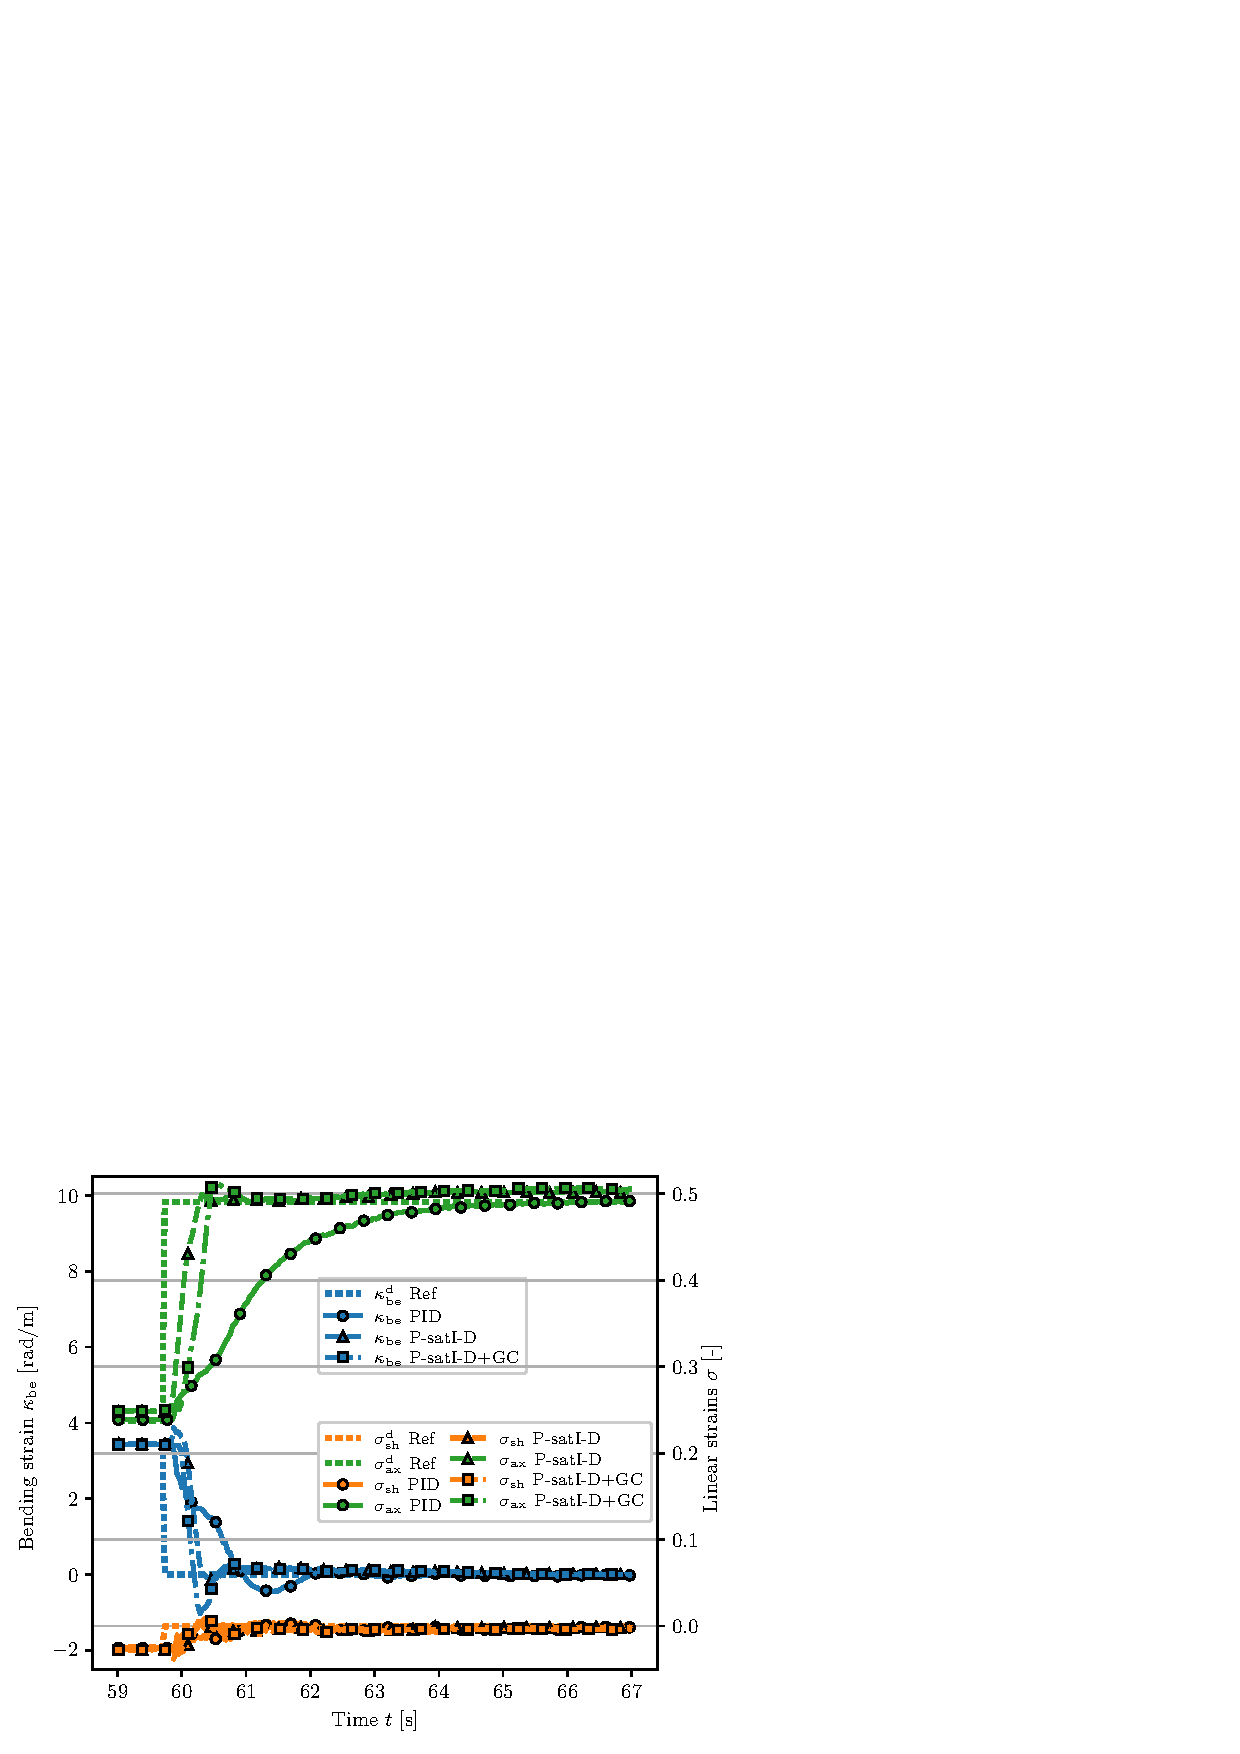
\includegraphics[width=0.49\columnwidth, trim={10, 10, 10, 10}]{hsacontrol/figures/experimental_results/configuration_space_regulation/fpu/fpu_step_response_q.pdf}\label{fig:hsacontrol:experimental_results:configuration_space_regulation:fpu:step_response:q}}
    \caption{Step response of the \emph{baseline PID}, \emph{P-satI-D} (with gravity compensation), and \emph{P-satI-D + GC} (with gravity cancellation) controllers on an FPU-based HSA robot.}\label{fig:hsacontrol:experimental_results:configuration_space_regulation:fpu:step_response}
\end{figure}

\begin{figure}[t]
    \centering
    \subfigure[End-effector position]{\includegraphics[width=0.32\columnwidth, trim={10, 10, 5, 10}]{hsacontrol/figures/experimental_results/configuration_space_regulation/fpu/20230925_092200_pee_three_panel_layout.pdf}\label{fig:hsacontrol:experimental_results:configuration_space_regulation:fpu:baseline_pid:pee}}
    \subfigure[Configuration]{\includegraphics[width=0.32\columnwidth, trim={10, 10, 10, 10}]{hsacontrol/figures/experimental_results/configuration_space_regulation/fpu/20230925_092200_q_three_panel_layout.pdf}\label{fig:hsacontrol:experimental_results:configuration_space_regulation:fpu:baseline_pid:q}}
    \subfigure[Control input]{\includegraphics[width=0.32\columnwidth, trim={10, 10, 10, 10}]{hsacontrol/figures/experimental_results/configuration_space_regulation/fpu/20230925_092200_phi_three_panel_layout.pdf}\label{fig:hsacontrol:experimental_results:configuration_space_regulation:fpu:baseline_pid:phi}}
    \caption{Experimental results for tracking a reference trajectory of eleven step functions with the baseline PID controller on an FPU-based HSA robot. \textbf{Panel (a):} End-effector position with the dotted and solid lines denoting the task-space reference and actual position, respectively.
    \textbf{Panel (b):} The planned (dotted) and the actual (solid) configuration. 
    \textbf{Panel (c):} The planned (dotted) and the actual (solid) actuation coordinates of the collocated system. 
    \textbf{Panel(d):} The saturated planar control inputs are visualized with solid lines, and the computed steady-state actuation with dotted lines.}\label{fig:hsacontrol:experimental_results:configuration_space_regulation:fpu:baseline_pid}
\end{figure}

\subsection{Implementation of closed-loop control}
Next, we implement the closed-loop control strategy laid out in Section~\ref{sub:hsacontrol:configuration_space_regulation:control_strategy}.
After evaluating the control law at a rate of \SI{40}{Hz} and saturating the control inputs to the ranges $[0, 3.40] \, \si{rad}$ for FPU and $[0, 4.71] \, \si{rad}$ for EPU, respectively, we map $\phi \in \mathbb{R}^2$ to desired positions of the four motors. For this, we consider the handedness of the \glspl{HSA} and apply the same actuation magnitude to both rods on the same side of the virtual backbone.
After tuning the gains for the feedback part of the model-based control laws in \eqref{eq:hsacontrol:gravity_compensation_controller} and \eqref{eq:hsacontrol:gravity_cancellation_controller}, we select $K_\mathrm{p} = \mathrm{diag}(0.3, 0.3)$, $K_\mathrm{i} = \mathrm{diag}(0.05, 0.05) \, \si{1 \per s}$, $K_\mathrm{d} = \mathrm{diag}(0.01, 0.01) \, \si{s}$, and $\gamma = \mathrm{diag}(100, 100)$. 
Furthermore, we report the performance of a model-free PID controller as a baseline. Here, the control input in task-space is given by $u_\mathrm{ts} = \begin{bmatrix}u_\mathrm{ts,x} & u_\mathrm{ts,y}\end{bmatrix}^\mathrm{T} = K_\mathrm{p}^\mathrm{PID} \, (p_\mathrm{ee}^\mathrm{d}-p_\mathrm{ee}) - K_\mathrm{d}^\mathrm{PID} \, \dot{p}_\mathrm{ee} + K_\mathrm{i}^\mathrm{PID} \int_0^t p_{\mathrm{ee},t'}^\mathrm{d} - p_{\mathrm{ee},t'} \: \mathrm{d}t'$, which is then mapped to the actuation via $\phi = \begin{bmatrix}
    u_\mathrm{ts,x}+u_\mathrm{ts,y}, & -u_\mathrm{ts,x}+u_\mathrm{ts,y}
\end{bmatrix}^\mathrm{T}$.
Here, we select $K_\mathrm{p}^\mathrm{PID} = \mathrm{diag}(10, 10) \, \si{rad \per m}$, $ K_\mathrm{i}^\mathrm{PID} = \mathrm{diag}(110, 110) \, \si{rad \per \meter \per \second}$, and $ K_\mathrm{d}^\mathrm{PID} = \mathrm{diag}(0.25, 0.25) \, \si{rad \, \second \per \meter}$.
\\

\begin{figure}[ht]
    \centering
    \subfigure[End-effector position]{\includegraphics[width=0.49\columnwidth, trim={5, 10, 5, 5}]{hsacontrol/figures/experimental_results/configuration_space_regulation/fpu/20230925_093236_pee.pdf}\label{fig:hsacontrol:experimental_results:configuration_space_regulation:fpu:p_sati_d:pee}}
    \subfigure[Configuration]{\includegraphics[width=0.49\columnwidth, trim={5, 10, 5, 5}]{hsacontrol/figures/experimental_results/configuration_space_regulation/fpu/20230925_093236_q.pdf}\label{fig:hsacontrol:experimental_results:configuration_space_regulation:fpu:p_sati_d:q}}\\
    \subfigure[Actuation coordinates]{\includegraphics[width=0.49\columnwidth, trim={5, 10, 5, 5}]{hsacontrol/figures/experimental_results/configuration_space_regulation/fpu/20230925_093236_varphi.pdf}\label{fig:hsacontrol:experimental_results:configuration_space_regulation:fpu:p_sati_d:varphi}}
    \subfigure[Control input]{\includegraphics[width=0.49\columnwidth, trim={5, 10, 5, 5}]{hsacontrol/figures/experimental_results/configuration_space_regulation/fpu/20230925_093236_phi.pdf}\label{fig:hsacontrol:experimental_results:configuration_space_regulation:fpu:p_sati_d:phi}}\\
    \caption{Experimental results for tracking a reference trajectory of eleven step functions with the P-satI-D controller on an FPU-based HSA robot. \textbf{Panel (a):} End-effector position with the dotted and solid lines denoting the task-space reference and actual position, respectively.
    \textbf{Panel (b):} The planned (dotted) and the actual (solid) configuration. 
    \textbf{Panel (c):} The planned (dotted) and the actual (solid) actuation coordinates of the collocated system. 
    \textbf{Panel(d):} The saturated planar control inputs are visualized with solid lines, and the computed steady-state actuation with dotted lines.}\label{fig:hsacontrol:experimental_results:configuration_space_regulation:fpu:p_sati_d}
\end{figure}

\begin{figure}[ht]
    \centering
    \subfigure[End-effector position]{\includegraphics[width=0.49\columnwidth, trim={5, 5, 5, 5}]{hsacontrol/figures/experimental_results/configuration_space_regulation/fpu/20230925_094023_pee.pdf}\label{fig:hsacontrol:experimental_results:configuration_space_regulation:fpu:p_sati_d_plus_gc:pee}}
    \subfigure[Configuration]{\includegraphics[width=0.49\columnwidth, trim={5, 5, 5, 5}]{hsacontrol/figures/experimental_results/configuration_space_regulation/fpu/20230925_094023_q.pdf}\label{fig:hsacontrol:experimental_results:configuration_space_regulation:fpu:p_sati_d_plus_gc:q}}\\
    \subfigure[Actuation coordinates]{\includegraphics[width=0.49\columnwidth, trim={5, 5, 5, 5}]{hsacontrol/figures/experimental_results/configuration_space_regulation/fpu/20230925_094023_varphi.pdf}\label{fig:hsacontrol:experimental_results:configuration_space_regulation:fpu:p_sati_d_plus_gc:varphi}}
    \subfigure[Control input]{\includegraphics[width=0.49\columnwidth, trim={5, 5, 5, 5}]{hsacontrol/figures/experimental_results/configuration_space_regulation/fpu/20230925_094023_phi.pdf}\label{fig:hsacontrol:experimental_results:configuration_space_regulation:fpu:p_sati_d_plus_gc:phi}}\\
    \caption{Experimental results for tracking a reference trajectory of eleven step functions with the P-satI-D + gravity cancellation controller on an FPU-based HSA robot. \textbf{Panel (a):} End-effector position with the dotted and solid lines denoting the task-space reference and actual position, respectively.
    \textbf{Panel (b):} The planned (dotted) and the actual (solid) configuration. 
    \textbf{Panel (c):} The planned (dotted) and the actual (solid) actuation coordinates of the collocated system. 
    \textbf{Panel(d):} The saturated planar control inputs are visualized with solid lines and the computed steady-state actuation with dotted lines.}\label{fig:hsacontrol:experimental_results:configuration_space_regulation:fpu:p_sati_d_plus_gc}
\end{figure}

\subsection{Evaluation}
We define a reference trajectory $p_\mathrm{ee}^\mathrm{d}(k), k \in \{ 1, \dots, n_k \}$ with a duration of \SI{110}{s} and consisting of eleven step functions as the reference trajectory.
We report the \gls{RMSE} metric $\sqrt{\sum_{k=1}^{n_k} \frac{\lVert p_\mathrm{ee}^\mathrm{d}(k) - p_\mathrm{ee}(k) \rVert_2^2}{n_k}}$ for assessing the control performance, where $p_\mathrm{ee}(k)$ is the actual trajectory of the end-effector.\\

\subsection{Results for controlling an FPU-based HSA robot}
The \emph{baseline PID} achieves an \gls{RMSE} of \SI{5.86}{mm} with respect to the reference trajectory. The \emph{P-satI-D} based on \eqref{eq:hsacontrol:gravity_compensation_controller} (with gravity compensation) exhibits an RMSE of \SI{4.17}{mm}. Similarly, the \emph{P-satI-D + GC} based on \eqref{eq:hsacontrol:gravity_cancellation_controller} (with gravity cancellation) displays an RMSE of \SI{4.13}{mm}.
We present a comparison of the three different controllers for a step response in Fig.~\ref{fig:hsacontrol:experimental_results:configuration_space_regulation:fpu:step_response} and plot the entire trajectories of the \emph{baseline PID} and the \emph{P-satI-D} in Figures~\ref{fig:hsacontrol:experimental_results:configuration_space_regulation:fpu:baseline_pid} and \ref{fig:hsacontrol:experimental_results:configuration_space_regulation:fpu:p_sati_d}, respectively.
Additionally, we discretize various continuous reference trajectories into setpoints: 
star trajectory ($873$ setpoints and duration of \SI{109}{s}), the flame of the TU Delft logo ($680$ setpoints and duration of \SI{85}{s}), the contour of the MIT-CSAIL logo ($1046$ setpoints and duration of \SI{131}{s}), and the outline of a bat at three different sizes ($1510$ setpoints and \SI{189}{s} duration).
The resulting Cartesian evolutions of the \emph{P-satI-D} controller tracking these continuous references are displayed in Fig.~\ref{fig:hsacontrol:experimental_results:configuration_space_regulation:fpu:task_space_trajectories}.

\begin{figure}[ht]
    \centering
    \subfigure[Star]{\includegraphics[width=0.32\columnwidth, trim={5, 5, 5, 5}]{hsacontrol/figures/experimental_results/configuration_space_regulation/fpu/20231019_072747_cartesian_evolution.pdf}\label{fig:hsacontrol:experimental_results:configuration_space_regulation:fpu:star}}
    \subfigure[TUD flame]{\includegraphics[width=0.32\columnwidth, trim={5, 5, 5, 5}]{hsacontrol/figures/experimental_results/configuration_space_regulation/fpu/20231019_081703_cartesian_evolution.pdf}\label{fig:hsacontrol:experimental_results:configuration_space_regulation:fpu:tud_flame}}
    \subfigure[MIT-CSAIL]{\includegraphics[width=0.32\columnwidth, trim={5, 5, 5, 5}]{hsacontrol/figures/experimental_results/configuration_space_regulation/fpu/20231019_082343_cartesian_evolution_with_logo.pdf}\label{fig:hsacontrol:experimental_results:configuration_space_regulation:fpu:mit_csail}}\\
    \subfigure[Bat trajectories]{\includegraphics[width=0.7\columnwidth, trim={5, 5, 5, 5}]{hsacontrol/figures/experimental_results/configuration_space_regulation/fpu/fpu_bats.pdf}\label{fig:hsacontrol:experimental_results:configuration_space_regulation:fpu:bats}}
    \caption{Cartesian evolution of the proposed P-sat-D controller (solid lines) tracking various continuous reference trajectories (dotted lines) on the FPU robot.
    % we compare the performance of the baseline PID, the model-based P-satI-D controller (with gravity compensation), P-satI-D + GC which also includes terms to cancel the gravitational effects.
    }\label{fig:hsacontrol:experimental_results:configuration_space_regulation:fpu:task_space_trajectories}
\end{figure}

\begin{figure}[hb]
    \centering
    % each picture has a size 575x575px
    \subfigure[t=\SI{0}{s}]{\includegraphics[width=0.192\columnwidth]{hsacontrol/figures/experimental_results/configuration_space_regulation/fpu/20231019_083240_overlayed_600x_cropped-0001-min.png}}
    \subfigure[t=\SI{47}{s}]{\includegraphics[width=0.192\columnwidth]{hsacontrol/figures/experimental_results/configuration_space_regulation/fpu/20231019_083240_overlayed_600x_cropped-0002-min.png}}
    \subfigure[t=\SI{94}{s}]{\includegraphics[width=0.192\columnwidth]{hsacontrol/figures/experimental_results/configuration_space_regulation/fpu/20231019_083240_overlayed_600x_cropped-0003-min.png}}
    \subfigure[t=\SI{141}{s}]{\includegraphics[width=0.192\columnwidth]{hsacontrol/figures/experimental_results/configuration_space_regulation/fpu/20231019_083240_overlayed_600x_cropped-0004-min.png}}
    \subfigure[t=\SI{188}{s}]{\includegraphics[width=0.192\columnwidth]{hsacontrol/figures/experimental_results/configuration_space_regulation/fpu/20231019_083240_overlayed_600x_cropped-0005-min.png}}
    \caption{Sequence of stills for the large bat trajectory performed with the P-satD controller on the FPU robot. The red and black dots visualize the desired and current end-effector positions, respectively. The past trajectory is plotted in red (reference) and black (actual). The blue line renders the shape of the virtual backbone.
    }\label{fig:hsacontrol:experimental_results:configuration_space_regulation:fpu:sequence_of_stills:bat}
\end{figure}

The step response in Fig.~\ref{fig:hsacontrol:experimental_results:configuration_space_regulation:fpu:step_response} shows how the two model-based controllers \emph{P-satI-D} and \emph{P-satI-D + GC} can leverage the planned $\phi^\mathrm{ss}$ and $q^\mathrm{d}$ to achieve a fast response time of roughly \SI{1.2}{s}. In contrast, the baseline PID needs to wait for the integral error to build up and thus has a much slower response time of approximately \SI{4.2}{s}. Furthermore, overshooting caused by the baseline PID is usually more extensive than that caused by the model-based controllers.
We conclude that \emph{P-satI-D} (gravity compensation) and \emph{P-satI-D + GC} (gravity cancellation) exhibit quite similar behavior. Sometimes, \emph{P-satI-D} exhibits undershooting at the beginning of the transient and \emph{P-satI-D + GC} overshooting towards the end of the transient (see Fig.~\ref{fig:hsacontrol:experimental_results:configuration_space_regulation:fpu:step_response:pee}).

\begin{figure}[ht]
    \centering
    \subfigure[End-effector position]{\includegraphics[width=0.47\columnwidth, trim={10, 10, 10, 10}]{hsacontrol/figures/experimental_results/configuration_space_regulation/epu/epu_step_response_chiee.pdf}\label{fig:hsacontrol:experimental_results:configuration_space_regulation:epu:step_response:pee}}
    \subfigure[Configuration]{\includegraphics[width=0.47\columnwidth, trim={10, 10, 10, 10}]{hsacontrol/figures/experimental_results/configuration_space_regulation/epu/epu_step_response_q.pdf}\label{fig:hsacontrol:experimental_results:configuration_space_regulation:epu:step_response:q}}
    \caption{Step responses of the \emph{baseline PID}, \emph{P-satI-D} (with gravity compensation), and \emph{P-satI-D + GC} (with gravity cancellation) controllers on an EPU-based HSA robot.}\label{fig:hsacontrol:experimental_results:configuration_space_regulation:epu:step_response}
\end{figure}

\begin{figure}[ht]
    \centering
    \subfigure[End-effector position]{\includegraphics[width=0.49\columnwidth, trim={5, 10, 5, 5}]{hsacontrol/figures/experimental_results/configuration_space_regulation/epu/20231019_143126_pee.pdf}\label{fig:hsacontrol:experimental_results:configuration_space_regulation:epu:p_sati_d:pee}}
    \subfigure[Configuration]{\includegraphics[width=0.49\columnwidth, trim={5, 10, 5, 5}]{hsacontrol/figures/experimental_results/configuration_space_regulation/epu/20231019_143126_q.pdf}\label{fig:hsacontrol:experimental_results:configuration_space_regulation:epu:p_sati_d:q}}\\
    \subfigure[Actuation coordinates]{\includegraphics[width=0.49\columnwidth, trim={5, 10, 5, 5}]{hsacontrol/figures/experimental_results/configuration_space_regulation/epu/20231019_143126_varphi.pdf}\label{fig:hsacontrol:experimental_results:configuration_space_regulation:epu:p_sati_d:varphi}}
    \subfigure[Control input]{\includegraphics[width=0.49\columnwidth, trim={5, 10, 5, 5}]{hsacontrol/figures/experimental_results/configuration_space_regulation/epu/20231019_143126_phi.pdf}\label{fig:hsacontrol:experimental_results:configuration_space_regulation:epu:p_sati_d:phi}}
    \caption{Experimental results for tracking a reference trajectory of eleven step functions with the P-satI-D controller on an EPU-based HSA robot. \textbf{Panel (a):} End-effector position with the dotted and solid lines denoting the task-space reference and actual position, respectively.
    \textbf{Panel (b):} The planned (dotted) and the actual (solid) configuration. 
    \textbf{Panel (c):} The planned (dotted) and the actual (solid) actuation coordinates of the collocated system. 
    \textbf{Panel(d):} The saturated planar control inputs are visualized with solid lines, and the computed steady-state actuation with dotted lines.}\label{fig:hsacontrol:experimental_results:configuration_space_regulation:epu:p_sati_d}
\end{figure}

\subsubsection{Results for controlling an EPU-based HSA robot}
Tracking the reference trajectory of eleven step functions with an EPU-based robot, the \emph{baseline PID} controller has an \gls{RMSE} of \SI{4.40}{mm}. The \emph{P-satI-D} (with gravity compensation) can able to achieve an \gls{RMSE} of \SI{3.63}{mm}. The \emph{P-satI-D + GC} controller exhibits similar performance(\gls{RMSE} of \SI{3.71}{mm}).
We visualize the step response of all three controllers in Fig.~\ref{fig:hsacontrol:experimental_results:configuration_space_regulation:epu:step_response} and the entire trajectory of the \emph{P-satI-D} controller in Fig.~\ref{fig:hsacontrol:experimental_results:configuration_space_regulation:epu:p_sati_d}.

Again, we notice that the response time of the model-based controllers (\SI{0.54}{s}) is much shorter than the response time of the baseline PID (\SI{3.84}{s}). Furthermore, the importance of a model-based control law is motivated by the oscillations in the transient of the baseline PID (see x-coordinate in Fig.~\ref{fig:hsacontrol:experimental_results:configuration_space_regulation:epu:step_response:pee}).
The steady-state error for the model-based controllers on the EPU material is slightly higher compared to the FPU material, as seen in Figures \ref{fig:hsacontrol:experimental_results:configuration_space_regulation:epu:step_response:pee} \& \ref{fig:hsacontrol:experimental_results:configuration_space_regulation:epu:p_sati_d:pee}. In Section~\ref{sub:hsamodel:planar_hsa_robot_model:model_verification}, we noticed that the shear model doesn't fully capture the actual system behavior. This then results in an error in the planned desired configuration $q^\mathrm{d}$, which the controller is not able to resolve because of the underactuation of the robot (see Fig.~\ref{fig:hsacontrol:experimental_results:configuration_space_regulation:epu:p_sati_d:q}).
\input{hsacontrol/sections/S03_operational_space_impedance_control}
\section{Experimental Insights}
This chapter presented two strategies for effective, model-based regulation of planar \gls{HSA} robots: the first proposes a configuration-space controller in conjunction with steady-state planning for mapping task-space setpoints to configuration-space setpoints, and the second introduces a operational space impedance controller.

\subsection{Configuration Space Regulation}

First, we introduced a configuration-space controller that combines an integral-saturated PID controller with a potential-shaping feedforward term.
The excellent agreement of the model with the actual system behavior (as shown in Sec.~\ref{sec:hsamodel:planar_hsa_robot_model}) enables our model-based controllers to perform very well at the task of setpoint regulation.
For the model-based controllers, any mismatch between the dynamic model and the actual system (as analyzed in Section~\ref{sub:hsamodel:planar_hsa_robot_model:model_verification}) has two impacts: (i) the steady-state planning provides us with a desired configuration $q^\mathrm{d}$ which the underactuated robot cannot achieve. This then, in turn, causes a small steady-state error in the end-effector position as seen for the manual setpoints in Fig.~\ref{fig:hsacontrol:experimental_results:configuration_space_regulation:fpu:p_sati_d:pee} \& \ref{fig:hsacontrol:experimental_results:configuration_space_regulation:fpu:p_sati_d_plus_gc:pee} 
and for the continuous references in Fig.\ref{fig:hsacontrol:experimental_results:configuration_space_regulation:fpu:task_space_trajectories}. This steady-state error is absent in the baseline PID as its integral term acts directly in task space. We suggest that future work include an integral term directly on the end-effector position to remove the remaining steady-state error of the model-based controller. Secondly, as (ii), model errors will lead to an offset in the planned steady-state actuation $\phi^\mathrm{ss}$. Therefore, applying a constant $\phi^\mathrm{ss}$ will not move the robot exactly to $p_\mathrm{ee}^\mathrm{d}$. As shown in Fig.~\ref{fig:hsacontrol:experimental_results:configuration_space_regulation:fpu:p_sati_d:phi}, the P-satI-D feedback term can compensate for this effect through its proportional and integral terms applied in the collocated variables \& \ref{fig:hsacontrol:experimental_results:configuration_space_regulation:fpu:p_sati_d_plus_gc:phi} 
As clearly seen in Fig.~\ref{fig:hsacontrol:experimental_results:configuration_space_regulation:fpu:p_sati_d:phi}, the control input drifts away from the planned $\phi^\mathrm{ss}$ to counteract the modeling errors.
In particular, for small to medium bending and axial strains, we observe a very good agreement between the model and the actual system behavior and, therefore, excellent control performance. 
The story slightly changes for more significant bend and twist angles. While the system identification showed that the expressiveness of the model was sufficient, we saw significant errors in our feedforward terms in some of our control experiments, which needed to be compensated by the P-satI-D feedback controller. Precisely, Fig.~\ref{fig:hsacontrol:experimental_results:configuration_space_regulation:fpu:p_sati_d:q} displays errors in the planned shear strain, which subsequently also leads to minor steady-state deviations in the x-coordinate of the end-effector as it can be seen in Fig.~\ref{fig:hsacontrol:experimental_results:configuration_space_regulation:fpu:p_sati_d:pee}. We hypothesize that these errors are mainly caused by the hysteresis characteristics of the \glspl{HSA}~\citep{good2022expanding}. This hypothesis is corroborated by the fact that we had to re-calibrate the axial rest strain $\sigma_\mathrm{ax}^0$ before the start of each experiment.

\subsection{Operational Space Impedance Control}
The Cartesian impedance controller, on the other hand, is designed to regulate the end-effector position directly and allows us to shape the impedance in operational space and, with that, fully preserve the softness of the robot.
It is, therefore, particularly suitable for applications where the robot interacts with the environment. For example, we will in Chapter~\ref{chp:braincontrol} demonstrate how the impedance controller can be combined with motor-imagery brain signals to guide the robot towards a desired position and how the impedance controller guarantees safety even when the setpoints are wrongly planned.
This impedance needs to be traded off with steady-state errors. We observed that the impedance controller is particularly sensitive to the model errors, as it does not have an integral term to compensate for them.


\section*{Afterword}
This chapter presented the first control strategies in literature for \gls{HSA} robots and verified them experimentally on two \gls{HSA} robot prototypes in the planar case.
Each of the two presented controllers offers unique advantages:
On the one hand, the configuration-space P-satI-D + potential shaping controller exhibits exceptional regulation accuracy, with minimal or no steady-state errors and exceptionally short response times.
Excitingly, follow-up work by \citet{soleti2025model} has extended and adapted this control approach to underactuated dielectric elastomer soft robots.
On the other hand, the operational space impedance controller complements the passive compliance of the soft robot with active compliance in the control strategy. It accomplishes this by eliminating integral terms that could pose potential safety hazards. Additionally, it enables us to precisely shape the stiffness of the closed-loop system in Cartesian space.
% In this chapter, we programmatically specified the setpoints of the regulation controller. When working towards a future where soft robots assist, for example, elderly people with activities of daily living, we are lacking, however, an effective \gls{HRI} approach. A \gls{BMI} would arguably represent the most direct and barrier-free \gls{HRI} approach for assisting with activities of daily living. For that reason, we investigate in Chapter~\ref{chp:braincontrol} the guidance of the operational space impedance controller with \gls{EEG}-based motor imagery.
In envisioning a future where soft robots assist elderly individuals with activities of daily living, an effective \gls{HRI} is paramount. While this chapter has focused on programmatically specifying setpoints for regulation controllers, we recognize a gap in how humans can intuitively command these robots. A \gls{BMI} emerges as a compelling solution, offering a direct and barrier-free interaction method that could significantly enhance the usability of assistive robotics. Consequently, in Chapter~\ref{chp:braincontrol}, we explore the feasibility of guiding an operational space impedance controller via \gls{EEG}-based motor imagery, aiming to create a more natural and accessible means of control of soft, and specifically \gls{HSA}, robots.
Furthermore, we illustrate how the Cartesian-space stiffness enables us to apply force in the desired directions (in this case, releasing hairspray by pressing a button with the end-effector) while maintaining the compliance and, consequently, the embodied intelligence of the soft robot in all other directions.
\chapter{Guiding Soft Robots with Motor-Imagery Brain Signals}
\label{chp:braincontrol}

\begin{abstract}
    Integrating Brain-Machine Interfaces into non-clinical applications like robot motion control remains difficult - despite remarkable advancements in clinical settings. Specifically, EEG-based motor imagery systems are still error-prone, posing safety risks when rigid robots operate near humans. This work presents an alternative pathway towards safe and effective operation by combining wearable EEG with physically embodied safety in soft robots. We introduce and test a pipeline that allows a user to move a soft robot's end effector in real time via brain waves that are measured by as few as three EEG channels. A robust motor imagery algorithm interprets the user's intentions to move the position of a virtual attractor to which the end effector is attracted, thanks to a new Cartesian impedance controller. We specifically focus here on planar soft robot-based architected metamaterials, which require the development of a novel control architecture to deal with the peculiar nonlinearities - e.g., non-affinity in control. We preliminarily but quantitatively evaluate the approach on the task of setpoint regulation. We observe that the user reaches the proximity of the setpoint in 66\% of steps and that for successful steps, the average response time is 21.5s. We also demonstrate the execution of simple real-world tasks involving interaction with the environment, which would be extremely hard to perform if it were not for the robot's softness.
\end{abstract}

\blfootnote{This chapter is partly based on \faFileTextO \, \faTrophy~\emph{\textbf{M. Stölzle}*, S. S. Baberwal*, D. Rus, S. Coyle, and C. Della Santina (2024). Guiding Soft Robots with Motor-Imagery Brain Signals and Impedance Control. In Proceedings of The 2024 IEEE 7th International Conference on Soft Robotics (RoboSoft) (pp. 1-8). IEEE}~\cite{stolzle2024guiding}.}


%% Start the actual chapter on a new page.
\newpage

\section{Introduction}
\glspl{BMI} \cite{liu2024cognitive} facilitate the translation of neural activity into actionable commands, enabling individuals to control external devices and systems through their thoughts and attention~\cite{coyle2007brain,lee2017brain}. Compared to traditional bulky EEG setups~\cite{van2012brain}, one of the emerging avenues towards practical and wearable \glspl{EEG} devices are systems based on motor imagery signals due to their intuitiveness and no external dependency on (e.g., visual) stimuli. These have been use in stroke rehabilitation \cite{khan2020review}. Several works in literature have considered using this technology to control robot manipulators~\cite{schiatti2017soft,aldini2019effect,lee2024noir}. % more citations: bhattacharyya2017motor, liu2018motor

However, the state-of-the-art classifiers on few-channel, online \gls{EEG} signals are still limited in achieving an accuracy of 65-75 \si{\percent}~\cite{arpaia2022non, lee2024noir} and are prone to producing outliers, which make it very challenging to operate robots safely and robustly using these techniques~\cite{liu2024cognitive}. In (rigid) robotics literature, this has been addressed by relying on force-based (i.e., impedance) control~\cite{schiatti2017soft} and by making the robot's behavior more predictable~\cite{aldini2019effect}.
%
%from a perspective of real-life scenarios along with several factors taken into consideration, such as a limited number of channels, operating an interface}~\textcolor{orange}{},
% Additionally, various factors such as the human brain being uncertain at times, low ITR rate,and low discrimination capacity of the human brain can inevitably lead to unintended movements and therefore pose a potential safety hazard to both humans and objects close to the robot.\textcolor{red}{!!!!{/cite}}
%
In this work, we follow a different path and investigate \textit{embodying} safety by pairing soft robots~\cite{rus2015design, della2020softencyclopedia} 
with \gls{BMI}. This way, risks can be mitigated, and more natural interactions with an unstructured environment can be achieved by relying on structural compliance.

\begin{figure*}
    \centering
    \includegraphics[width=0.95\textwidth]{braincontrol/figures/control_scheme/control_scheme_v2_cropped.pdf}
    \caption{Scheme of the proposed approach to control HSA robots with motor imagery. Brain signals steer an attractor in operational space: first, we switch the active coordinate axis when we detect jaw clenching. If no jaw clenching is detected, we classify the EEG signals based on left/right motor imaginations into positive and negative movements along the active axis. Next, we regulate the robot towards the chosen attractor position $x^\mathrm{at}$ with a Cartesian impedance controller. This controller first cancels all static forces and the residual coupling of the null space on the operational space dynamics. This allows us to now shape our own potential with a PD term in operational space. As the robot is underactuated, we optimize least-squares to identify the actuation $\phi^\mathrm{d}$ so that the residual between the desired and actual torques in the configuration space is minimized. Icons created by Flaticon\copyright.}
    \label{fig:braincontrol:control_scheme}
\end{figure*}

While \gls{BMI}-based assistance has been investigated with a focus on 
% exoskeletons~\cite{wairagkar2016movement, araujo2021development} 
soft exosuits assisting hand-rehabilitation ~\cite{zhang2019eeg} or with strenuous arm acitivites~\cite{tacca2022neuro}, 
% \textcolor{red}{TODO: insert combination of a) soft robotics and BCI are both emerging fields, b) most of the focus has been on binary decisions }
it is still an open challenge how \gls{BMI} can be used for controlling soft manipulators. 
%One key reason for existing strategies developed for soft exosuits and hands not being directly applicable to more complex soft robots is that those strategies restricted the interface to binary decisions such as \emph{open} / \emph{close}. To overcome these limitations, 
In this work, we make a first step towards solving this challenge by proposing a pipeline (see Fig. \ref{fig:braincontrol:control_scheme}) that lets the user steer the soft robot's end-effector in Cartesian space. The two key ingredients are a novel mapping strategy transforming the brain signals into meaningful references and Cartesian impedance control. The latter is essential because it allows for preserving the robot's compliance in closed-loop \cite{della2017controlling}. We build the proposed \gls{BMI} pipeline around a \gls{HSA} soft robot \cite{stolzle2023modelling, stolzle2024experimental}, % truby2021recipe
which relies on architected metamaterials and electrical actuation to elongate, bend, and twist. This makes the control problem especially challenging because of the peculiarity of these systems' dynamics, namely underactuation and non-affinity in control. We provide more details on innovation from the model-based control standpoint in Section~\ref{sub:braincontrol:computational_controller}.
 
We quantitatively verify the entire approach on mind-controlled setpoint regulation involving tracking a reference consisting of nine-step functions and demonstrate the qualitative behavior when assisting with a simple daily living activity. 
Furthermore, we compare the performance of our motor imagery-based control to approaches giving the computational controller access to the privileged information of setpoints, which can considered to be an upper bound on performance.
%Furthermore, we compare the performance of our motor imagery-based control to approaches that can be considered an upper bound on performance: (a) control using keyboard inputs and (b) giving the computational controller access to the privileged information of setpoints.
% This control strategy now allows us to define the stiffness of the closed-loop system in Cartesian space. We verify the controller on the task of pressing the button of a perfume, which requires high stiffness in the normal direction of the interaction and flexibility in the tangential direction, allowing the soft robots to adapt to the environment interaction with physical intelligence.

Our contributions are: (i) Establishing a \gls{BMI} strategy for continuum soft robots. This strategy is supported by experiments in which we perform setpoint regulation with a planar \gls{HSA} robot and motor imagery, (ii) A Cartesian impedance controller for \gls{HSA} robots, which we experimentally validated on a simple \gls{ADL} task involving environment interaction: the user needs to steer the end-effector towards the tip of a hairspray container, apply force for releasing the fluid, and finally let the robot retreat from the contact.          

A video attachment to this paper including recordings of experimental results can be found on YouTube\footnote{\url{https://youtu.be/wZTOxBPZmPc}}.
Furthermore, we have open-sourced our code including the OpenVibe pipeline on GitHub\footnote{\url{https://github.com/tud-phi/sr-brain-control}}.
\section{Task-space Impedance Control}
In this work, we let the user steer with motor imaginary brain signals the Cartesian position $x \in \mathbb{R}^2$ of the end-effector (i.e., the platform) of a planar \gls{HSA} robot.
We realize this strategy by first classifying the motor imaginary signals into Cartesian-space movement directions (e.g., the active axis and sign of the movement). We use this information to adjust the position of a task-space attractor iteratively (see Section~\ref{sub:braincontrol:planning_attractors_switching}). Section~\ref{sub:braincontrol:computational_controller} describes how a model-based computational controller establishes this attractor. Importantly, we preserve the soft robot's compliance by shaping the closed-loop system's impedance in Cartesian space.


\subsection{Background: Motor Imagery-based BMI systems}\label{sub:braincontrol:motor_imagery_bmi}

Imagining the movement of body parts or limbs (e.g., hands, legs, tongue) without moving it or the mental rehearsal of a motor act without overt movement execution is termed Motor Imagery~\cite{lotze2006motor}.  The neuronal activities observable inside a frequency range of \SI{8}{Hz} to \SI{12}{Hz} (Mu) and \SI{12}{Hz} to \SI{30}{Hz} (Beta) are associated with cortical areas directly connected to the brain’s motor output (activating primary sensorimotor areas that can be modulated with imaginary mental movement in healthy as well people with neuromuscular disabilities). 
% Motor Imagery is widely used for the BMI systems involved in either task-specific for instance exoskeleton /cite!!, or motion wheelchair /cite!!.

The motor imagery \gls{BMI} framework typically consists of four integral components:

\begin{enumerate}
    \item \textbf{Signal acquisition:} The initial stage involves the recording of neural signals while the person imagines the movements of the limbs, generally acquired using noninvasive methodologies (e.g., \gls{EEG}).
    \item \textbf{Feature extraction:} Following signal acquisition, signal processing techniques are applied to extract salient features from the neural patterns associated with specific cognitive processes or intentions.
    \item \textbf{Feature translation:} This translation phase interprets the user's cognitive intent, converting it into actionable instructions for external devices.
    \item \textbf{Device output:} The culmination of the \gls{BMI} process is the application of the interpreted commands to external devices. 
    % \glspl{BMI} can be employed in various applications, ranging from motor control tasks, such as wheelchair navigation, to text input and the orchestration of complex robotic exoskeletons.
\end{enumerate}

As detailed further in Sec.~\ref{sub:braincontrol:bmi_protocol}, we leverage the difference in signals when imagining motor actions vs. rest state to control the sign of movement. The active axis of movement can be switched by clenching the jaw. % More details about the \gls{BMI} protocol can be found in Section .
% To demonstrate the proof of concept, in our work, we focus on Motor Imagery imagination v/s rest state which is used as a control, further described in Section \ref{sub:braincontrol:bmi_protocol}

% \subsection{Planning attractors with brain signals (multi-class)}\label{sub:braincontrol:planning_attractors_multiclass}
% We classify the \gls{EEG} signals into \textcolor{orange}{four classes: move left ($u=(1, 0)$), move right ($u=(-1, 0)$), move down ($u=(0, 1)$), and move up ($u=(0, -1)$)}. More details about the procedure used to process and classify \gls{EEG} signals can be found in Section~\ref{ssub:braincontrol:eeg_pipeline}.
% Subsequently, this information is used to manipulate an attractor position $x^\mathrm{at} \in \mathbb{R}^2$, which is later tracked by a computational controller (see Section~\ref{sub:braincontrol:computational_controller}). The following policy is used to update the attractor at each time step $k$:
% \begin{equation}
%     x^\mathrm{at}(k) = x^\mathrm{at}(k-1) + \Delta_\mathrm{x} \, u(k),
% \end{equation}
% where $\Delta_\mathrm{x}$ is a tunable constant influencing the velocity of the attractor.

\subsection{Planning attractors with brain signals}\label{sub:braincontrol:planning_attractors_switching}
Our brain signal processing pipeline provides us with two pieces of information at each time step $k$: i) the unit vector $e_\mathrm{a}(k) \in \{ [1, 0]^\mathrm{T}, [0, 1]^\mathrm{T} \}$ corresponding to the current active axis of movement % with $\lVert e^\mathrm{at} \rVert = 1$
and ii) the sign of movement $s(k) \in \{ -1, 1 \}$. We use $e_\mathrm{a}(k)$ and $s(k)$ to incrementally steer a virtual attractor defined in operational space $x^\mathrm{at} \in \mathbb{R}^2$ as follows
%
%The following policy is used to update the attractor at each time step $k$:
\begin{equation}
    u(k) = s(k) \, e_\mathrm{a}(k) \in \mathbb{R}^2, \quad  x^\mathrm{at}(k) = x^\mathrm{at}(k-1) + \Delta_\mathrm{x} \, u(k),
\end{equation}
where $\Delta_\mathrm{x} \in \mathbb{R}^+$ is a tunable constant influencing the velocity of the attractor movement.
%
Later, we will shape the potential field with a computational controller such that the attractor becomes a globally asymptotically stable equilibrium (see Section~\ref{sub:braincontrol:computational_controller}).

\begin{figure}
\begin{center}
    \includegraphics[width=\columnwidth]{braincontrol/figures/eeg_pipeline/eeg_pipeline_v3_compressed.pdf}
    \caption{EEG data processing pipeline: The EEG data is acquired in real-time, pre-processed, and divided into episodes and subbands. Next, we extract power features and pass them to two LDA classifiers: the first outputs the axis of movement (for example, moving along the x- or y-axis), and the second provides the sign of movement (for example, positive or negative movement along the active axis). These commands are then used to move the attractor in Cartesian space.}
    \label{fig:braincontrol:eeg_pipeline}
\end{center}
\end{figure}

\subsection{Background: modeling planar HSA robots}
Robots based on \glspl{HSA} rely on rods made of architected metamaterials to generate motion.  % ~\cite{truby2021recipe}
More specifically, twisting the rods along their handedness leads to an elongation of the rod~\cite{good2022expanding}. Combining multiple \glspl{HSA} in the setting of a parallel robot and actuating them with servo motors allows us to generate complex motion primitives and offer beneficial mechanical characteristics such as a high stiffness-to-weight ratio~\cite{stolzle2023modelling, good2022expanding}.

Prior work~\cite{stolzle2024experimental} has shown that the shape of planar \gls{HSA} robots can be approximated by one \gls{CS} segment. Therefore, we define the configuration of the system as $q = \begin{bmatrix}
    \kappa_\mathrm{be} & \sigma_\mathrm{sh} & \sigma_\mathrm{ax}
\end{bmatrix}^\mathrm{T} \in \mathbb{R}^3$.
We also have access to closed-form formulations of the forward kinematics $\pi: q \rightarrow \chi$ and inverse kinematics $\varrho: \chi \rightarrow q$ where $\chi = \begin{bmatrix}
    x^\mathrm{T} & \theta
\end{bmatrix}^\mathrm{T} \in SE(2)$ is the pose in task space and $\theta$ represents the end-effector orientation~\cite{stolzle2024experimental}.
We use the notation $J(q) = \frac{\partial x}{\partial q} \in \mathbb{R}^{2\times3}$ to refer to the kinematic Jacobian.

We can then derive the dynamics of the planar \gls{HSA} robot in Euler-Lagrangian form
\begin{equation}\label{eq:braincontrol:configuration_space_dynamics}
    M(q) \Ddot{q} + C(q,\dot{q})\dot{q} + G(q) + K \, (q-q^0) + D \, \dot{q} = \alpha(q,\phi),
\end{equation}
where $M(q), C(q,\dot{q}) \in \mathbb{R}^{3 \times 3}$ captures the inertial and Coriolis effects, $G(q) \in \mathbb{R}^3$ contributes the gravitational forces and $K \in \mathbb{R}^{3 \times 3}$ is the stiffness of the robot in its un-actuated state $q^0$. Furthermore, $D \in \mathbb{R}^{3 \times 3}$ is a positive-definite damping matrix. Finally, for the planar case, two \gls{HSA} rods are assumed to be actuated by the motor/twist angle $\phi \in \mathbb{R}^2$. As the handedness of the rods will be accounted for later, we state the actuation bounds as $0 \leq \phi_i \leq \phi_\mathrm{max} \: \forall i \in \{ 1, 2 \}$.
The auxetic trajectory~\cite{good2022expanding} causes the motors to act through the elasticity of the rods on the system and modify the axial rest length of the rod as a function of the twist strain~\cite{stolzle2023modelling}.
Furthermore, the stiffness of the rod can be modeled to be an affine function with respect to the twist strain~\cite{good2022expanding, stolzle2023modelling}. Both effects are captured in the actuation function $\alpha(q,\phi)$, which is nonlinear with respect to the actuation coordinate $\phi$ and affine in the configuration $q$.
%
Although this has never been done in the context of HSA robots, it is immediate to see that their dynamics \eqref{eq:braincontrol:configuration_space_dynamics} can be projected into operational space yielding the form~\cite{della2019exact, della2020model} % khatib1987unified
\begin{equation}\label{eq:braincontrol:operational_space_dynamics}
    \Lambda(q) \, \Ddot{x} + \mu(q,\dot{q}) \dot{q} + J_\mathrm{B}^{+\mathrm{T}} ( G(q) + K (q-q^0) + D \, \dot{q} ) = J_\mathrm{B}^{+\mathrm{T}} \alpha(q,\phi),
\end{equation}
where $J_\mathrm{B}^+(q) = B^{-1}J^\mathrm{T}(J B^{-1} J^\mathrm{T})^{-1} \in \mathbb{R}^{3\times2}$ is the dynamically consistent pseudo-inverse, $\Lambda(q) = (J \, B^{-1} J^\mathrm{T})^{-1} \in \mathbb{R}^{2 \times 2}$ is the inertia matrix in task space, and $\mu(q, \dot{q}) = \Lambda(q) \, (J B^{-1} C - \dot{J}) \in \mathbb{R}^{2 \times 3}$ collects the Cartesian Coriolis and centrifugal terms. % ~\cite{khatib1987unified}

\subsection{Cartesian impedance controller}\label{sub:braincontrol:computational_controller}
In previous work~\cite{stolzle2024experimental}, we have devised a model-based control strategy for regulating a planar \gls{HSA} robot towards a desired position in task space. %We propose here a new strategy that overcomes several limitations of that previous work which are critical for the application discussed in this paper - namely: (i) it involves a complex and computationally demanding planning procedure for identifying a suitable setpoint in configuration space, (ii) our configuration-space controller contains integral terms, making it unsafe for environment interactions, and (iii) it is based on a compensation of static forces in configuration-space thus not allowing us to shape the impedance characteristics in operational space.
%
We introduce below a novel control strategy that addresses some limitations of our previous work that are critical for the \gls{BMI} application. Namely, we (i) avoid computationally demanding planning procedures, (ii) remove integral terms that are unsafe for environment interaction, and (iii) enable impedance shaping in operational space. This Cartesian-space impedance controller is inspired by ~\cite{ott2008cartesian,della2020model}, but specifically designed for and tailored to \gls{HSA} robots. Crucially, we need to overcome the challenges of underactuation and the nonlinearity in the actuation - which were not present in that original work. %We, therefore, solve online a least-squares optimization problem, identifying the optimal actuation for generating the demanded task space forces.

\subsubsection{Proposed controller}
% We implement an operational space impedance action~\cite{ott2008cartesian, della2020model} that renders $x^\mathrm{at}$ an attractor of the closed-loop system.
We propose the following dynamic feedback law that renders $x^\mathrm{at}$ an attractor of the closed-loop system %~\cite{ott2008cartesian, della2020model} 
\begin{equation}\label{eq:braincontrol:cartesian_impedance_controller}
\begin{split}
    \tau =& \: J^\mathrm{T}(q) \, \left (K_x \, (x^\mathrm{at} - x) - D_x \, \dot{x} \right ) + G(q) + K \, (q-q^0)\\
    & \: + J^\mathrm{T}(q) \, J_\mathrm{B}^{+\mathrm{T}}(q) \, D \, \dot{q} + J^\mathrm{T}(q) \, \mu(q,\dot{q}) \left ( I_3 - J_\mathrm{B}^+(q) J(q) \right )\dot{q}
\end{split}
\end{equation}
where $\tau \in \mathbb{R}^3$ is the desired torque in configuration space, $G(q) + K \, (q-q^0)$ cancels the acting gravitational and elastic forces, and $J^\mathrm{T} J_\mathrm{B}^{+\mathrm{T}} D \, \dot{q}$ removes the natural dissipation in operational space.
We emphasize that because the system is underactuated, we need to cancel the stiffness directly in the configuration instead of operational space as done in previous work~\cite{della2020model}.
We can shape our desired impedance characteristics in Cartesian space with the PD term $f_\mathrm{PD} = K_x \, (x^\mathrm{at} - x) - D_x \, \dot{x} $ which is then projected into configuration space by premultiplying with $J^\mathrm{T}(q)$.

The term $\mu(q,\dot{q}) \left ( I_3 - J_\mathrm{B}^+(q) J(q) \right )\dot{q}$ decouples the operational space dynamics from the residual of the null-space dynamics~\cite{della2020model}\cite[Ch. 4]{ott2008cartesian}.
The identity $\dot{q} = J_\mathrm{B}^+ \, \dot{x} + Z^\mathrm{T} \, \nu_\mathrm{N}$, where $Z^\mathrm{T} \in \mathbb{R}^{3 \times 1}$ is the dynamically-consistent pseudo-inverse of the null space, allows us to formulate $\dot{q}$ as a sum of the task-space velocity $\dot{x}$ and the null-space velocity $\nu_\mathrm{N}$. Leveraging this identity, the Coriolis and centrifugal matrix $\mu(q,\dot{q})$ can be split into a term $\mu_x(q,\dot{q}) = \mu \, J_\mathrm{B}^+ \in \mathbb{R}^{2 \times 2}$ excited by $x$ and the expression $\mu_\mathrm{N}(q,\dot{q}) = \mu \, Z^\mathrm{T} \in \mathbb{R}^{2 \times 1}$ that is excited by the null-space coordinates resulting in $\mu(q,\dot{q}) \, \dot{q} = \mu_x(q,\dot{q}) \, \dot{x} + \mu_\mathrm{N}(q,\dot{q}) \, \nu_\mathrm{N}$.
This allows us to cancel the term $\mu_\mathrm{N}(q,\dot{q}) \, \nu_\mathrm{N}$ through $\mu(q,\dot{q}) \left ( I_3 - J_\mathrm{B}^+(q) J(q) \right )\dot{q}$ without having to compute the null space explicitly.


% The first step consists of establishing a PD feedback in Cartesian space
% \begin{equation}
%     f =  K_x \, (x^\mathrm{at} - x) - D_x \, \dot{x} + J_\mathrm{B}^{+\mathrm{T}} \, D \, \dot{q}. % + \eta(q, \dot{q}) J_\mathrm{B}^+ \left (G(q) + K \, q \right ).
% \end{equation}
% where $K_x \in \mathbb{R}^{2\times2}$ is the designed task-space stiffness and $D_x % \in \mathbb{R}^{2\times2}$ adds dissipation.
% We make use of the kinematic Jacobian to project the designed task-space force into % configuration space and additionally establish cancellation of the gravitational and % elastic forces with
% \begin{equation}
%     \tau = \alpha(q,\phi) = J^\mathrm{T}(q) \, f + G(q) + K \, (q-q^0).
% \end{equation}

In summary, the closed-loop dynamics in operational space can be stated as
\begin{equation}\label{eq:braincontrol:closed_loop_dynamics}
    \Lambda(q) \, \Ddot{x} + \mu(q,\dot{q}) \, J_\mathrm{B}^+ \, \dot{x} + K_x \, (x^\mathrm{at} - x) - D_x \, \dot{x} = 0,
\end{equation}
which results in $x^\mathrm{at}$ being the globally asymptotically stable equilibrium of the operational space dynamics.

% \begin{figure}
%     \centering
%     \includegraphics[width=0.85\columnwidth, trim={10 10 10 10}]{braincontrol/figures/workspace/operational_workspace_fpu_with_ee.pdf}
%     \caption{Operational workspace of a HSA robot with attached end-effector: the color displays the mean steady-state actuation $\frac{\phi_1^\mathrm{ss} + \phi_2^\mathrm{ss}}{2}$ necessary for the end-effector to remain at the position. Additionally, we visualize three example shapes: the straight configuration with $\phi^\mathrm{ss} = (0, 0)$ (blue), maximum clockwise bending with $\phi^\mathrm{ss} = (3.49, 0) \, \si{rad}$ (red), and maximum counter-clockwise bending with $\phi^\mathrm{ss} = (0, 3.49) \, \si{rad}$ (green).}
%     \label{fig:braincontrol:hsa_workspace}
% \end{figure}

\begin{figure*}
\begin{center}
    \subfigure[Operational workspace]{\includegraphics[width=0.36\linewidth]{braincontrol/figures/workspace/operational_workspace_fpu_with_ee.pdf}\label{fig:braincontrol:hsa_workspace}}
    \subfigure[Experimental setup]{\includegraphics[width=0.63\linewidth]{braincontrol/figures/experimental_setup/experimental_setup_v3_cropped.pdf}\label{fig:braincontrol:experimental_setup}}
    \caption{\textbf{Panel (a:} Operational workspace of a HSA robot with attached end-effector: the color displays the mean steady-state actuation $\frac{\phi_1^\mathrm{ss} + \phi_2^\mathrm{ss}}{2}$ necessary for the end-effector to remain at the position. Additionally, we visualize three example shapes: the straight configuration with $\phi^\mathrm{ss} = (0, 0)$ (blue), maximum clockwise bending with $\phi^\mathrm{ss} = (3.49, 0) \, \si{rad}$ (red), and maximum counter-clockwise bending with $\phi^\mathrm{ss} = (0, 3.49) \, \si{rad}$ (green).
    \textbf{Panel (b):} The HSA robot is mounted platform-down to a motion capture cage with 8x Optitrack PrimeX 13 cameras, which track the 3D pose of the platform (i.e., the end-effector). A Dynamixel MX-28 servo actuates each of the four HSAs. We project a rendering of the current (white dot) and desired (red dot) end-effector position, the attractor (green square), and the operational workspace (grey area) onto the black screen in the background. The study subject wears a cap with the Neuroconcise FlexEEG sensor, and we acquire the data of three electrodes connected to the motor cortex.}
\end{center}
\end{figure*}

\begin{figure}
\begin{center}
    \includegraphics[width=0.85\columnwidth]{braincontrol/figures/eeg_pipeline/ERDS.pdf}
    \caption{ERD/S (overall average) over a time period of \SI{2.5}{s} of training data for right-hand Imagination v/s rest state including the Alpha and Beta bands of the EEG signals  where the cue is presented at \SI{0}{s}. We plot the data of three sensors (i.e., channels): FC3-CP3 (left), FCZ-CPZ (middle) and FC4-CP4 (right).}
    \label{fig:braincontrol:ERDS}
\end{center}
\end{figure}

\begin{figure*}[t]
    \centering
    \subfigure[End-effector x-coordinate]{\includegraphics[width=0.47\textwidth, trim={5, 5, 5, 5}]{braincontrol/figures/setpoint_regulation/20231031_185546_pee_x.pdf}\label{fig:braincontrol:experimental_results:setpoint_regulation:brain:pee_x}}
    \subfigure[End-effector y-coordinate]{\includegraphics[width=0.47\textwidth, trim={5, 5, 5, 5}]{braincontrol/figures/setpoint_regulation/20231031_185546_pee_y.pdf}\label{fig:braincontrol:experimental_results:setpoint_regulation:brain:pee_y}}\\
    \subfigure[Configuration $q$]{\includegraphics[width=0.47\textwidth, trim={5, 5, 5, 5}]{braincontrol/figures/setpoint_regulation/20231031_185546_q.pdf}\label{fig:braincontrol:experimental_results:setpoint_regulation:brain:q}}
    \subfigure[Control input $\phi$]{\includegraphics[width=0.47\textwidth, trim={5, 5, 5, 5}]{braincontrol/figures/setpoint_regulation/20231031_185546_phi.pdf}\label{fig:braincontrol:experimental_results:setpoint_regulation:brain:phi}}
    \caption{Experimental results for tracking a reference trajectory of nine step functions with motor imagery. \textbf{Panel (a) \& (b):} The x/y-coordinate of the end-effector position with the solid line denoting the actual position, the dotted line the attractor position, and the dashed line the reference (i.e., the setpoint).
    \textbf{Panel (c):} The evolution of the configuration.
    \textbf{Panel(d):} The saturated planar control inputs. }\label{fig:braincontrol:experimental_results:setpoint_regulation:brain}
\end{figure*}

\subsubsection{Mapping to Lagrangian forces}
%
Now that we have formulated our control law $\tau$ in configuration space, we need to identify a strategy to specify the motor angles $\phi \in \mathbb{R}^2$ such that $\alpha(q,\phi) \approx \tau$. Note that, in contrast to other continuum soft robots studied in literature~\cite{della2023model}, the actuation term $\alpha(q,\phi)$ is not affine in control. %, but rather a nonlinear function with respect to the actuation coordinates $\phi$. 
%Therefore, mapping configuration-space torques to motor commands is not straightforward.
In previous work~\cite{stolzle2024experimental}, we side-stepped this challenge by linearizing with respect to the steady-state actuation $\phi^\mathrm{ss}$: $A(q) = \lVert \frac{\partial \alpha}{\partial \phi}\rVert_{\phi=\phi^\mathrm{ss}}$ therefore recovering the usual scenario of an affine actuation function. Unfortunately, this is not possible in the setting of this work as i) we do not have access to such $\phi^\mathrm{ss}$, and ii) linearizing around $\phi$ causes the closed-loop system to become unstable. We, therefore, propose to formulate instead a nonlinear least-squares problem $\phi^\mathrm{d} = \argmin_\phi \frac{1}{2} \lVert \tau - \alpha(q,\phi) \rVert^2$ and solve it in real-time with a Levenberg Marquardt solver implemented in JAX~\cite{jaxopt_implicit_diff}.

We note that this approach is not guaranteed to be valid for the general case of an underactuated soft robot but for this particular structure of $\alpha(q,\phi) \in \mathbb{R}^3$ with $\phi \in \mathbb{R}^2$ it is possible to identify solutions $\phi$ with the Euclidean norm of the residual being smaller than $0.001$.
The source code of the controller is available on GitHub\footnote{\url{https://github.com/tud-phi/hsa-planar-control}}.
% Next, the actuation vector is linearized with respect to the current twist angle $A_\phi(q) = \frac{\partial \alpha}{\partial \phi} \big|_{\phi} \in \mathbb{R}^{3 \times 2}$. With that, we now have
% \begin{equation}
%     J^\mathrm{T} f = \alpha(q,\phi) + A_\phi(q) \, u
% \end{equation}
\section{Experiments}

\subsection{Experimental setup}
In the following, we detail the \gls{EEG} data processing procedure (see also Fig.~\ref{fig:braincontrol:eeg_pipeline}) and present our experimental setup, which is annotated in Fig.~\ref{fig:braincontrol:experimental_setup}.

\subsubsection{EEG data processing}\label{ssub:braincontrol:eeg_pipeline}
We integrate the 3-channel flexEEG Neuroconcise device with the OpenVibe software
% through a Lab Streaming Layer (LSL) 
to acquire the EEG data and process it in real-time.
This configuration facilitates data recording and cue presentation. We process the \gls{EEG} signals at a sampling frequency of \SI{125}{Hz} with a pipeline that involves three bi-polar channels around the motor cortex: FC3-CP3, FCZ-CPZ, and FC4-CP4.
After a notch filter of \SI{50}{Hz}, we apply Independent Component Analysis (ICA) to extract three independent components from the recorded \gls{EEG} data, which is represented by the equation $S(t) = W \, X(t)$, where $S(t)$ are the extracted independent components and $W$ represents the unmixing matrix, allowing us to separate eye blink artifacts in \gls{EEG} signals, which is critical for enhancing the accuracy. 
Subsequently, we apply a Butterworth filter bank to isolate specific frequency bands of interest, including 8-15 \si{Hz} and 15-42 \si{Hz}. 
% removed because of space constraints
% The general equation for a Butterworth filter of order $N$ for a given frequency range (e.g., 8-15 \si{Hz}) is
% \begin{equation}
%     H(f) = \frac{1}{{1 + \left(\frac{f}{f_\mathrm{c}}\right)^{2N}}},
% \end{equation}
% where $H(f)$ represents the frequency response of the filter, $f$ is the frequency of the \gls{EEG} signal, $N$ is the filter order, and $f_\mathrm{c}$ is the critical frequency (i.e., center frequency) of the desired frequency band.
This enhances the ability to analyze \gls{EEG} data by isolating and examining different frequency band components within the \gls{EEG} signals. Once the signals are filtered in sub-bands and epoched with a duration of \SI{2}{s} and time interval of \SI{0.065}{s}, the features are extracted by the log of the power: $L_i(t) = \log\left(P_i(t)\right)$, where the power $P_i(t) = |E_i(t)|^2$ is represented by square of magnitude of the \gls{EEG} signal $E_i(t)$ at time instance $t$.
These features are then provided to a classifier, which we select as \gls{LDA} due to its simplicity~\cite{lotte2014tutorial}.

We implement a second classifier with the same pipeline, where jaw clenching is provided as a muscle artifact that is classified v/s raw EEG data. 
\subsubsection{Robotic system}
% HSA robot
We consider a robot consisting of four \gls{HSA} rods, which were 3D printed via digital projection lithography % ~\cite{truby2021recipe} 
from the photopolymer resin Carbon FPU 50. % ~\cite{carbon:fpu50}.
Each \gls{HSA} rod is electrically actuated by a Dynamixel M-28 servo up to a maximum twist angle of $\phi_\mathrm{max} = \SI{3.49}{rad}$.
% MoCap
The robot is attached platform-down to a motion capture cage with eight Optitrack Prime X13 cameras tracking at \SI{200}{Hz} the pose of reflective markers attached to the end-effector of the \gls{HSA} robot.
We estimate the current Cartesian-space velocity of the end-effector with a Savitzky-Golay filter. 
Subsequently, we leverage a closed-form expression of the inverse kinematics of a \gls{CS} model~\cite{stolzle2023experimental} to compute the current configuration $q$ of the robot.
% projector
We render an image of the current shape of the robot together with the present end-effector position (white dot), the attractor planned by the user (green square), the operational workspace (grey, see also Fig.~\ref{fig:braincontrol:hsa_workspace}) and if applicable, the goal position (red dot). 
We specify the currently active axis of movement $e_\mathrm{a}$ with a double arrow and project the resulting image onto a black screen in the background of the motion capture cage.
% control/software architecture
The robot is operated with a ROS2 software framework\footnote{\url{https://github.com/tud-phi/ros2-hsa}}. We receive the predicted and classified brain signals via TCP at a frequency of \SI{18}{Hz} and move the attractor subsequently with $\Delta_\mathrm{x} = \SI{0.2}{mm}$. We evaluate the Cartesian impedance controller using the gains $K_\mathrm{p} = \SI{300}{N \per m}$, $K_\mathrm{d} = \SI{1.5}{N s \per \meter}$ at a frequency of \SI{50}{Hz} and finally send the desired motor positions to the servos.

% latency computation
% FlexEEG device
% For 24bit and 250 Hz, the time between packets is 47ms.
% transit time between FlexEEG and pc is ~35ms
% OpenVibe data processing and classification
% running at 125Hz, so maximum latency of 8ms
% joylike operation
% queries the TCP connection at 100Hz, therefore maximum delay of 10ms
% computational control loop
% runs at 50Hz, so maximum delay of 20ms
% communication with dynamixel motors
% dual-way communication works at 100Hz, so maximum delay (solely based on communication) of 10ms
The entire control pipeline from measuring \gls{EEG} signals to sending the actuation commands to the motors exhibits a maximum latency of (i.e., is upper-bounded by)  \SI{130}{ms}.

\subsection{BMI protocol:}\label{sub:braincontrol:bmi_protocol}
In the following, we will describe the protocol for collecting the motor imagery dataset, training the \gls{EEG} classifiers, and mapping classifier outputs into actionable robot commands.

\subsubsection{Training protocol}

The participant is given brief instructions about motor imagery signals.
We follow the Graz-BCI~\cite{roc2021review} paradigm, which assists with training, where the display of the cue instructs the participant to perform imagination of movements: when a left arrow appears, the participant is asked to rest and not focus on motor movement. When the right arrow appears on the screen, the participant is asked to imagine the motor activity from the dominant hand (here, the right hand), such as grasping or squeezing an object. The training protocol for right-hand motor imagery v/s rest demands fifty cues per class. 
We similarly collect data for the second classifier by asking participants to clench their jaw, which can be detected as muscular artifacts (vs. no muscular movement) in the \gls{EEG} signals.
At the end of the trial, we train both classifiers (see Sections~\ref{sub:braincontrol:motor_imagery_bmi} and \ref{ssub:braincontrol:eeg_pipeline} for more information) and repeat the procedure until an accuracy of \SI{75}{\percent} is obtained for right-hand motor imagery v/s rest and accuracy of \SI{85}{\percent} for jaw clench artifact v/s raw EEG.


% \definecolor{adaee4ed-88c8-5b21-a9e7-31316ebef86f}{RGB}{255, 179, 178}
% \definecolor{f3551e38-74df-57e2-b793-83d7fe876c85}{RGB}{0, 0, 0}
% \definecolor{0b71a967-1f15-55a5-9bb9-70efa7b4fc58}{RGB}{51, 51, 51}
% \definecolor{58712c6c-1b6d-5716-9834-102aad6341dc}{RGB}{175, 179, 255}
% \definecolor{70af333d-4869-5f2a-97ca-9904a9fce6c3}{RGB}{179, 254, 174}
% \definecolor{747aec21-333b-59ee-84e3-ddff893e5ccd}{RGB}{255, 216, 176}
% \definecolor{5856d031-3da1-575c-834e-c77e9e438c62}{RGB}{162, 177, 195}
% \tikzstyle{512bdd77-c3aa-5669-a956-85f7a90c6fb4} = [rectangle, rounded corners, minimum width=3cm, minimum height=1cm, text centered, font=\normalsize, color=0b71a967-1f15-55a5-9bb9-70efa7b4fc58, draw=f3551e38-74df-57e2-b793-83d7fe876c85, line width=1, fill=adaee4ed-88c8-5b21-a9e7-31316ebef86f]
% \tikzstyle{7f27e395-8473-5b8a-b568-31425bce482a} = [trapezium, trapezium left angle=70, trapezium right angle=110, minimum width=3cm, minimum height=1cm, text centered, font=\normalsize, color=0b71a967-1f15-55a5-9bb9-70efa7b4fc58, draw=f3551e38-74df-57e2-b793-83d7fe876c85, line width=1, fill=58712c6c-1b6d-5716-9834-102aad6341dc]
% \tikzstyle{e78ae073-3d46-5489-8262-483c8269c0e6} = [diamond, minimum width=3cm, minimum height=2cm, text centered, font=\normalsize, color=0b71a967-1f15-55a5-9bb9-70efa7b4fc58, draw=f3551e38-74df-57e2-b793-83d7fe876c85, line width=1, fill=70af333d-4869-5f2a-97ca-9904a9fce6c3]
% \tikzstyle{69bbb168-da59-5865-902f-94e77902bf95} = [rectangle, minimum width=3cm, minimum height=1cm, text centered, font=\normalsize, color=0b71a967-1f15-55a5-9bb9-70efa7b4fc58, draw=f3551e38-74df-57e2-b793-83d7fe876c85, line width=1, fill=747aec21-333b-59ee-84e3-ddff893e5ccd]
% \tikzstyle{7be24b85-97d0-5b76-ba9e-d94005dca8f2} = [thick, draw=5856d031-3da1-575c-834e-c77e9e438c62, line width=2, ->, >=stealth]

% \begin{center}
% \begin{tikzpicture}[node distance=2cm]
% \node (start) [start] {Start};
% \node (training) [training, below of=start] {Training (no feedback)};
% \node (testing) [testing, below of=training] {Testing (with feedback)};
% \node (decision) [decision, below of=testing, yshift=-0.5cm] {Accuracy \textgreater 65?};
% \node (action) [action, below of=decision, yshift=-0.5cm] {HSA control real time};
% \draw [arrow] (start) -- (training);
% \draw [arrow] (training) -- (testing);
% \draw [arrow] (testing) -- (decision);
% %\draw [arrow] (training) -- (decision);
% \draw [arrow] (decision) -- node[anchor=east] {Yes} (action);
% \draw [arrow] (decision.east) -| ++(0.8,0.8) node[above right] {No} |- (testing.east);
% \label{Flowchart}
% \end{tikzpicture}
% \end{center}
% \begin{minipage}{\linewidth} 
% \captionsetup{justification=centering, singlelinecheck=false}
% \captionof{figure}{Protocol design of the Real-time HSA robots control}
% \end{minipage} 

% \begin{figure*}[t]
%     \centering
%     \subfigure[End-effector x-coordinate]{\includegraphics[width=0.47\textwidth, trim={5, 5, 5, 5}]{braincontrol/figures/setpoint_regulation/20231031_181745_pee_x.pdf}\label{fig:braincontrol:experimental_results:setpoint_regulation:keyboard:pee_x}}
%     \subfigure[End-effector y-coordinate]{\includegraphics[width=0.47\textwidth, trim={5, 5, 5, 5}]{braincontrol/figures/setpoint_regulation/20231031_181745_pee_y.pdf}\label{fig:braincontrol:experimental_results:setpoint_regulation:keyboard:pee_y}}\\
%     \subfigure[Configuration $q$]{\includegraphics[width=0.47\textwidth, trim={5, 5, 5, 5}]{braincontrol/figures/setpoint_regulation/20231031_181745_q.pdf}\label{fig:braincontrol:experimental_results:setpoint_regulation:keyboard:q}}
%     \subfigure[Control input $\phi$]{\includegraphics[width=0.47\textwidth, trim={5, 5, 5, 5}]{braincontrol/figures/setpoint_regulation/20231031_181745_phi.pdf}\label{fig:braincontrol:experimental_results:setpoint_regulation:keyboard:phi}}
%     \caption{Experimental results for tracking a reference trajectory of nine step functions with keyboard inputs. \textbf{Panel (a) \& (b):} The x/y-coordinate of the end-effector position with the solid line denoting the actual position, the dotted line the attractor position, and the dashed line the reference (i.e., the setpoint).
%     \textbf{Panel (c):} The evolution of the configuration.
%     \textbf{Panel(d):} The saturated planar control inputs. }\label{fig:braincontrol:experimental_results:setpoint_regulation:keyboard}
% \end{figure*}

\begin{figure*}[t]
    \centering
    \subfigure[End-effector x-coordinate]{\includegraphics[width=0.47\textwidth, trim={5, 5, 5, 5}]{braincontrol/figures/setpoint_regulation/20231030_181558_pee_x.pdf}\label{fig:braincontrol:experimental_results:setpoint_regulation:computational:pee_x}}
    \subfigure[End-effector y-coordinate]{\includegraphics[width=0.47\textwidth, trim={5, 5, 5, 5}]{braincontrol/figures/setpoint_regulation/20231030_181558_pee_y.pdf}\label{fig:braincontrol:experimental_results:setpoint_regulation:computational:pee_y}}\\
    \subfigure[Configuration $q$]{\includegraphics[width=0.47\textwidth, trim={5, 5, 5, 5}]{braincontrol/figures/setpoint_regulation/20231030_181558_q.pdf}\label{fig:braincontrol:experimental_results:setpoint_regulation:computational:q}}
    \subfigure[Control input $\phi$]{\includegraphics[width=0.47\textwidth, trim={5, 5, 5, 5}]{braincontrol/figures/setpoint_regulation/20231030_181558_phi.pdf}\label{fig:braincontrol:experimental_results:setpoint_regulation:computational:phi}}
    \caption{Experimental results for tracking a reference trajectory of nine step functions directly with the Cartesian impedance controller with access to the privileged information $x^\mathrm{d}$. \textbf{Panel (a) \& (b):} The x/y-coordinate of the end-effector position with the solid line denoting the actual position, the dotted line the attractor position, and the dashed line the reference (i.e., the setpoint).
    \textbf{Panel (c):} The evolution of the configuration.
    \textbf{Panel(d):} The saturated planar control inputs. }\label{fig:braincontrol:experimental_results:setpoint_regulation:computational}
\end{figure*}


\subsubsection{Online robot control}
Now, the participant operates the HSA robot in real time, with both classifiers being executed online.
Moreover, we map the outputs of the classifier into actionable commands: we initialize the x-axis as the active axis of movement (i.e., $e_\mathrm{a} = [1,0]$). When the first classifier detects jaw clenching for at least \SI{80}{\percent} of samples over a duration of \SI{2.8}{s}, we switch to the y-axis: $e_\mathrm{a} = [0,1]$ and vice-versa. If we do not detect any jaw clenching artifacts, we evaluate the output of the second classifier in parallel: if there is motor imagery activity identified in the \gls{EEG} classifier, the attractor will be moved in the positive direction (i.e., $s=1$) along $e_\mathrm{a}$. In contrast, if the \gls{EEG} signals are classified as the participant being at rest, $s=-1$ (i.e., movement in the negative direction).

% ~\footnote{\url{https://www.neuroconcise.co.uk/}}.

\subsection{Setpoint regulation}\label{sub:braincontrol:experiments:setpoint_regulation}
We randomly generate nine setpoints $x^\mathrm{d}(t) \in \mathbb{R}^2$ within the operational workspace of the robot (see Fig.~\ref{fig:braincontrol:hsa_workspace} and display them as a red circle to the user over a duration of \SI{540}{s}.
The user can freely move the attractor to reach and keep the end-effector at the setpoint.
% In addition to the motor imagery-based control, we conduct experiments where the subject controls the robot with a keyboard.
% As a keyboard is a very efficient and precise \gls{HMI}~\textcolor{red}{TODO Sonal: add a citation if you can find one}, this represents an upper bound on the performance we could expect from the \gls{BCI}.
% Here, the space button is used to switch that axis of movement $e_\mathrm{a}$ and positive/negative movement can be controlled via the left/right arrows.
Furthermore, we execute an experiment in which the computational controller has access to normally privileged information: as we substitute $x^\mathrm{at}$ with $x^\mathrm{d}$ in \eqref{eq:braincontrol:cartesian_impedance_controller}, the Cartesian impedance controller now immediately regulates the robot towards the setpoint.
By excluding the \gls{BMI} from the pipeline, this provides us with a reference of the performance we can expect from the computational controller and, with that, also represents a performance upper bound.

% sequence of stills with 10 images
\begin{figure*}[tb]
    \centering
    \subfigure[$t=\SI{0}{s}$]{\includegraphics[width=0.192\textwidth]{braincontrol/figures/adl_task/20231031_203004_trimmed_and_cropped-0001-min.png}}
    \subfigure[$t=\SI{12}{s}$]{\includegraphics[width=0.192\textwidth]{braincontrol/figures/adl_task/20231031_203004_trimmed_and_cropped-0002-min.png}}
    \subfigure[$t=\SI{24}{s}$]{\includegraphics[width=0.192\textwidth]{braincontrol/figures/adl_task/20231031_203004_trimmed_and_cropped-0003-min.png}}
    \subfigure[$t=\SI{36}{s}$]{\includegraphics[width=0.192\textwidth]{braincontrol/figures/adl_task/20231031_203004_trimmed_and_cropped-0004-min.png}}
    \subfigure[$t=\SI{48}{s}$]{\includegraphics[width=0.192\textwidth]{braincontrol/figures/adl_task/20231031_203004_trimmed_and_cropped-0005-min.png}}\\
    \subfigure[$t=\SI{60}{s}$]{\includegraphics[width=0.192\textwidth]{braincontrol/figures/adl_task/20231031_203004_trimmed_and_cropped-0006-min.png}}
    \subfigure[$t=\SI{72}{s}$]{\includegraphics[width=0.192\textwidth]{braincontrol/figures/adl_task/20231031_203004_trimmed_and_cropped-0007-min.png}}
    \subfigure[$t=\SI{84}{s}$]{\includegraphics[width=0.192\textwidth]{braincontrol/figures/adl_task/20231031_203004_trimmed_and_cropped-0008-min.png}}
    \subfigure[$t=\SI{96}{s}$]{\includegraphics[width=0.192\textwidth]{braincontrol/figures/adl_task/20231031_203004_trimmed_and_cropped-0009_edited-min.png}\label{fig:braincontrol:experimental_results:adl_task_sequence_of_stills:spraying}}
    \subfigure[$t=\SI{108}{s}$]{\includegraphics[width=0.192\textwidth]{braincontrol/figures/adl_task/20231031_203004_trimmed_and_cropped-0010-min.png}}
    \caption{Sequence of stills for completing a basic Activity of Daily Living (ADL) by controlling the robot with EEG-based motor imagery.
    \emph{Note: }Fig.~\ref{fig:braincontrol:experimental_results:adl_task_sequence_of_stills:spraying} is edited for improved contrast.
    }\label{fig:braincontrol:experimental_results:adl_task:sequence_of_stills}
\end{figure*}

\subsection{Interacting with the environment on a real-world task}\label{sub:braincontrol:experiments:adl}
We consider the \gls{ADL} task of releasing hairspray by actuating the button of its container with the \gls{HSA} robot's end-effector. For successful execution, the end-effector must be very stiff in the normal direction of the contact. On the other hand, we might want to benefit from the physical intelligence of the system by being relatively flexible in the tangential direction. Therefore, we first define the perpendicular stiffness $k_\perp = \SI{500}{N\per\meter}$ and the tangential stiffness as $k_\parallel = \SI{50}{N \per \meter}$. We assume that the normal direction of the contact can be described by the polar angle $\theta_\perp$ (with respect to the x-axis). We envision that in the future, the user can adjust such stiffness characteristics online via a \gls{BMI} system similar to~\cite{schiatti2017soft}. In this work, however, we estimate by visual inspection that $\theta_\perp=\SI{1.31}{rad}$.
The Cartesian stiffness matrix in global coordinates is then given by $K_x = R(\theta_\perp) \, \mathrm{diag}(k_\perp, k_\parallel) \, R(\theta_\perp)^\mathrm{T}$
where $R(\theta_\perp) \in SO(2)$ is the rotation matrix between global and contact frames.
% Analog to the setpoint regulation task, the user can move the attractor freely in Cartesian space when executing the described \gls{ADL} task.

\begin{figure*}[tb]
    \centering
    \subfigure[End-effector $x$-coordinate]{\includegraphics[width=0.47\textwidth, trim={5, 5, 5, 5}]{braincontrol/figures/adl_task/20231031_203004_pee_x.pdf}\label{fig:braincontrol:experimental_results:adl_task:brain:pee_x}}
    \subfigure[End-effector $y$-coordinate]{\includegraphics[width=0.47\textwidth, trim={5, 5, 5, 5}]{braincontrol/figures/adl_task/20231031_203004_pee_y.pdf}\label{fig:braincontrol:experimental_results:adl_task:brain:pee_y}}
    \\
    \subfigure[Configuration $q$]{\includegraphics[width=0.47\textwidth, trim={5, 5, 5, 5}]{braincontrol/figures/adl_task/20231031_203004_q.pdf}\label{fig:braincontrol:experimental_results:adl_task:brain:q}}
    % \subfigure[Joy signal $u$]{\includegraphics[width=0.49\textwidth, trim={5, 5, 5, 5}]{braincontrol/figures/adl_task/20231031_203004_joy_signal.pdf}\label{fig:braincontrol:experimental_results:adl_task:brain:u}}
    \subfigure[Control input $\phi$]{\includegraphics[width=0.47\textwidth, trim={5, 5, 5, 5}]{braincontrol/figures/adl_task/20231031_203004_phi.pdf}\label{fig:braincontrol:experimental_results:adl_task:brain:phi}}
    \caption{Experimental results for completing a basic Activity of Daily Living (ADL) by controlling the robot with EEG-based motor imagery. \textbf{Panel (a) \& (b):} The x/y-coordinate of the end-effector with the solid line and dotted lines denoting the actual and attractor position, respectively.
    \textbf{Panel (c):} The evolution of the configuration.
    % \textbf{Panel (c):} The joy commands $u$ derived from the classified brain signals used to move the attractor in Cartesian space.
    \textbf{Panel(d):} The saturated planar control inputs. }\label{fig:braincontrol:experimental_results:adl_task:brain}
\end{figure*}

\subsection{Evaluation metrics}
% Look at this paper for evaluation metrics: ~\cite{rakshit2020hybrid}
In the following, we will introduce and define a few metrics that help us assess the performance of the approach.

\subsubsection{Event-Related Synchronization/De-Synchronization:}
We apply \gls{ERD} / \gls{ERS}~\cite{pfurtscheller1999event} to demonstrate the difference between \gls{EEG} signals when the participant imagines right-hand movement vs. rest, i.e., no activity. \gls{ERD}/\gls{ERS} corresponds to a shift in power during imagination with respect to a baseline. It is defined by
\begin{equation}
    \mathrm{ERD/ERS}(t, f) = \frac{P(t, f) - P_{\mathrm{base}}(f)}{P_{\mathrm{base}}(f)},
\end{equation}
where $\mathrm{ERD/ERS}(t, f)$ represents the \gls{ERD} or \gls{ERS} at a specific time $t$ and frequency $f$, $P(t, f)$ stands for the power of brain activity during imagination, and $P_\mathrm{base}(f)$ denotes the baseline power. 

\subsection{Step response metrics}
For the task of setpoint regulation, we analyze primarily two aspects: (a) is the participant able to reach the proximity of setpoint within the (generously) allotted time of \SI{60}{s}? We define the proximity of the setpoints as $\lVert x^\mathrm{d} - x(t)\rVert_2 \leq \SI{2}{mm}$. And (b) what is the response time for reaching for the first time the proximity of the setpoint?
\section{Results and Discussion}\label{sec:braincontrol:results_and_discussion}

First, we analyze the \gls{ERD}/\gls{ERS} behavior with respect to rest vs. motor imaginations in Fig.~\ref{fig:braincontrol:ERDS}. It is evident that the baseline of rest remained the same in both scenarios when the participant did not perform motor imagery, but as soon as the cue is presented at \SI{0.0}{s}, a shift in power for the right-hand motor imagery with comparison to rest state is noticeable. 

We present the results for setpoint regulation employing motor imagery in Fig.~\ref{fig:braincontrol:experimental_results:setpoint_regulation:brain}. 
We observe that the participant can reach the proximity of the setpoint within the allotted time of \SI{60}{s} six out of nine times (i.e., \SI{66.6}{\percent}).
For the successful steps, the average response time is \SI{21.5}{s}.
However, as our protocol does not contain a command to let the attractor rest, it is challenging to keep the end-effector at the setpoint and we observe oscillations, particularly with respect to the x-coordinate.
From the results in Fig.~\ref{fig:braincontrol:experimental_results:setpoint_regulation:keyboard}, it is evident that a keyboard is a superior \gls{HMI}. It only takes the participant two setpoints to get familiar with the interface, and afterwards, the performance displayed is excellent.
However, for instance, for people with limb impairment, or people with Spinal Cord Injury (SCI), such an interface is inaccessible and, therefore, only represents an upper bound of what we strive to achieve with \gls{BCI} systems.
% In our third experiment, we ask the Cartesian impedance controller to track the setpoints directly.
% The fast response time, a well-known characteristic of model-based control approaches, is evident. However, the errors in the model (for example, caused by hysteresis or unmodelled nonlinearities)~\citep{stolzle2024experimental}, together with the lack of integral action, lead to steady-state errors. % They are especially pronounced for the y-coordinate.

Finally, we consider the \gls{ADL} task of releasing hair spray using the end-effector of the \gls{HSA} robot. We present a sequence of stills in Fig.~\ref{fig:braincontrol:experimental_results:adl_task:sequence_of_stills} and plots of the entire sequence in Fig.~\ref{fig:braincontrol:experimental_results:adl_task:brain}.
Already during the first attempt, the participant can steer the end-effector toward the button, apply force, and release the fluid within \SI{86}{s}.
The impedance of the controller is clearly visible in Fig.~\ref{fig:braincontrol:experimental_results:adl_task:brain:pee_y} when the manipulator is in contact with the object at time \SI{74}{s} to \SI{104}{s}.
Also, we noticed that the end-effector does not need to be perfectly aligned with the center of the button and can still complete the task successfully due to the compliance of the closed-loop system in the tangential direction.

We noticed that the variability of setting up the \gls{EEG} device on each study participant and the \gls{EEG} sensor noise caused by external factors (e.g., floor vibrations) still pose a considerable challenge for deploying motor imagery-based tools in practice. Furthermore, subject-specific factors such as the ability to focus on imagining motor actions, mental tiredness, etc., significantly affected the performance (e.g., classification accuracy, setpoint tracking error).
\section{Conclusion}
In this chapter, we proposed to combine motor imagery-based \gls{BMI} systems with continuum soft robots. This symbiosis promises the safe and compliant operation of robots that can assist people with limb impairments in their daily lives.
While the binary motor imagery classifier achieves an accuracy of only $\approx \SI{70}{\percent}$, we demonstrated experimentally its effectiveness through assistance with an activity of daily living and safe operation.
As demonstrated in the \gls{ADL} experiment, the physical intelligence of the soft robot can compensate for errors and deviations in the output of the \gls{BMI} classifier.
% Furthermore, we introduced a Cartesian impedance controller for planar \gls{HSA} robots that can deal with the peculiar characteristics of these robots (e.g., underactuation, non-affinity in control, etc.), and allows for model-based control without interfering with the structural compliance of the system.

% For future work, we suggest running a user study that includes a diverse group of non-expert subjects, and a more diverse set of soft robots.
% Furthermore, we it would be interesting to deploy the methodology on soft robots with more \glspl{DOF}, such as, for example, the Helix soft robot~\citep{guan2023trimmed}.
% Finally, relying on \gls{SOTA} \gls{EEG} classifiers, such as CTNet~\citep{zhao2024ctnet}, might increase the classification accuracy and ultimately allow for full 3D spatial brain control of the soft robot's task space motion - including the addition of a \emph{rest} mode which would allow the end-effector to remain at a pose.
For future work, we recommend conducting a user study with a diverse group of non-expert participants and incorporating a broader range of soft robots. Connected, it would be interesting to apply this methodology to soft robots with more \glspl{DOF}, such as the Helix soft robot~\citep{guan2023trimmed}. Finally, utilizing \gls{SOTA} \gls{EEG} classifiers like CTNet~\citep{zhao2024ctnet} could improve classification accuracy and ultimately enable full 3D spatial brain control of the soft robot’s task space motion—including the addition of a \emph{rest} mode to keep the end-effector at a fixed pose.

\section*{Acknowledgment}
The authors would like to thank Dr. Fabien Lotte for his suggestions concerning the protocol, Dr. Tomas Ward and the Neuroconcise team for their support with the FlexEEG device, and J.K Balasubramanian for his assistance with the EEG setup.

% \chapter{Piston-Driven Pneumatically-Actuated Soft Robots: Modeling and Backstepping Control}
\chapter{Backstepping Control of Piston-Driven Pneumatically-Actuated Soft Robots}
\label{chp:backstepping}

\begin{abstract}
    Actuators' dynamics have been so far mostly neglected when devising feedback controllers for continuum soft robots since the problem under the direct actuation hypothesis is already quite hard to solve. Directly considering actuation would have made the challenge too complex. However, these effects are, in practice, far from being negligible. The present chapter focuses on model-based control of piston-driven pneumatically-actuated soft robots. We propose a model of the relationship between the robot's state, the acting fluidic pressure, and the piston dynamics, which is agnostic to the chosen model for the soft system dynamics. 
    We show that backstepping is applicable even if the feedback coupling of the outer on the inner subsystem is not linear.
    Thus, we introduce a general model-based control strategy based on backstepping for soft robots actuated by fluidic drive. As an example, we derive a specialized version for a robot with piecewise constant curvature. 
\end{abstract}

\blfootnote{This chapter is based on \faFileTextO~\emph{\textbf{M. Stölzle}, C. Della Santina (2021). Piston-driven pneumatically-actuated soft robots: Modeling and backstepping control. IEEE Control Systems Letters, 6, 1837-1842.}~\cite{stolzle2021piston}.
}


%% Start the actual chapter on a new page.
\newpage

\section{Introduction}\label{sec:backstepping:introduction}
% \dropcap{C}{ontinuum} soft robots are systems entirely made of deformable materials, so to resemble the trunk of an elephant~\citep{della2020softencyclopedia}. 
% Controlling continuum soft robots is challenging because of the infinite amount of Degrees of Freedom (DoFs), the multi-body dynamics, nonlinear potentials, underactuation, and the high degree of uncertainties~\citep{george2018control}. 
% Combining feedback controllers % (inherently robust to model uncertainties)
% and simplified dynamical models can help taming this complexity and achieve good experimental performance \citep{thieffry2018control, della2020model, franco2021energy}.
%
%many approaches investigated the use of the constant curvature assumption and its extensions for static and dynamic control for continuum soft robotic manipulators~\citep{della2020model}.

%
%\citep{falkenhahn2014trajectory} proposes an optimal dynamic controller for pneumatically actuated manipulators which estimates an optimal trajectory that reduces the transition time and actuator jerk. Similarly, \citep{marchese2016dynamics} describes a trajectory optimization scheme for a soft planar manipulator. Clearly, there is need to not only incorporate the actuator dynamics into the trajectory planning, but also in the actual joint control. 

% Related work
% types of fluidic actuators

%While the actuator dynamics are often negligible for tendon-driven robots, the actuator dynamics of pneumatic actuators are slower and more nonlinear~\citep{george2018control}. 

% modeling
\dropcap{A}ccurate low-dimensional models of the continuum dynamics have been thoroughly investigated in recent years~\citep{faure2012sofa, grazioso2019geometrically, sadati2021tmtdyn}, serving as the base for model-based controllers \citep{boyer2020dynamics, della2023model}. 
In comparison, researchers have devoted little or no attention to modeling the actuator dynamics, despite this being far from a negligible effect in practice, in particular for pneumatic actuation. %Consider for example pneumatic actuation \citep{x}. 
%Simplified linear models 
%To the best of the authors' knowledge, the only work explicitly dealing with this challenge is \citep{wang2017soft}, which proposes a simplified model for a soft robotic gripper.
%
% In contrast, fewer publications investigate the modeling of the kinematics and dynamics of the mapping from actuation to configuration space. \citep{wang2017soft} proposes a simplified dynamic model for soft robotic grippers by considering the  deformation in a two-dimensional plane and dividing the Fluidic Elastomer Actuator (FEA) into a sequence of $n$ line segments with constant length. Viscoelastic joints are used to connect the segments with the bending motion generated by chamber expansion modeled by a series of rotational torques acting on each joint. The Euler-Lagrangian equation is used to derive the dynamics of the system of segments.  Experiments show a almost linear relationship between applied air pressure and bending angles for some FEAs while other FEAs incorporate slight nonlinear behaviours~\citep{wang2017soft}.
%
%Fluidic drive cylinders can have certain advantages over other fluidic energy supplies such as solenoid valves as for the fact that the segment curvature is monotonically related to the cylinder displacement, there is no exchange of fluid with the environment and the fluid flow can be continuously adjusted~\citep{marchese2016design}.
%
% PID controllers
The lack of models pairs with the scarcity of model-based dynamic controllers. Existing strategies only rarely reason on the actuators' dynamics, if not through simple heuristics.
%
For example, \citep{lindenroth2016stiffness, marchese2016design, della2020model} use a combination of PID control and inversion of quasi-static linear approximations to compensate for the actuators' dynamics.
%
This strategy may present clear limitations in terms of performance and stability assessment.
%
%to relate the desired torque in configuration space $\Bar{\tau}$ to a commanded actuation sequence of solenoid valves or to the actuation of pneumatic pistons. %A cascaded control approach is applied with an inner PID loop controlling pistons, and an outer loop controlling the curvature of the arm in~\citep{marchese2014design}. 
%
% Even when PID controllers work, well %because of the mostly linear relationship between chamber pressure and robot configuration for a limited pressure range~\citep{lindenroth2016stiffness}, 
% the gains are intricate to tune, and sensitive to changes in the robot design or actuator parameters.
%
% As an alternative, \citet{gillespie2016simultaneous} propose a data-driven approach combined with an MPC controller.
% This sometimes works reasonably well as some experiments show a mostly linear relationship between chamber pressure and robot configuration for a limited pressure range~\citep{lindenroth2016stiffness}.
% 
% \citet{marchese2014design, marchese2016design} models the the dynamics of a pneumatic drive cylinder and the relationship between the change in fluid pressure inside the chambers of the arm segment and the pressure in the fluidic drive cylinder as a parameter of wall resistance and the compliance of elastomeric channels. Further, they also model the force output of an electric linear actuator to drive the fluidic cylinder dependent on the input motor voltage. This model however, is not used for control purposes and their controller relies on a cascaded control feedback algorithm with an inner PID loop running at \SI{1}{kHz} to control the position of the linear actuator and an outer loop executed at \SI{20}{Hz} to control the curvature of the arm segment by adapting the demanded piston position~\citep{marchese2014design}.

% sliding mode controller
% Sliding mode controllers based on second order lumped system dynamics have been explored to control a soft pneumatic actuator through the means of solenoid valves~\citep{skorina2015feedforward}. 
% The sliding mode controller was bench-marked against an additional feedforward term. The sliding mode controller together with the feedforward term shows the best tracking performance.

\begin{figure}[t]
  \centering
  \includegraphics[width=0.9\columnwidth]{backstepping/figures/backstepping_graphics_control_scheme_v3_cropped.pdf}
  \caption{Schematic block diagram of the proposed nonlinear backstepping controller for a pneumatically-actuated soft robot. The approach considers both the fluidic drive cylinder and the soft system dynamics. It is agnostic to the chosen soft system controller in configuration-space $\tau(q,\dot{q})$.}\label{fig:backstepping:control_scheme}
\end{figure}

As model-based control of soft robots becomes a mature discipline, the need for general ways of dealing with actuators' dynamics becomes more pressing. In this chapter, we deal with this challenge by following a backstepping approach, which is an established strategy to deal with dynamical systems with a triangular structure. %We focus on piston-driven pneumatically-actuated soft robots.
%
A pneumatic model based on the ideal gas law is derived, and the pneumatic actuation system is compensated in a quasi-static fashion in \citet{falkenhahn2016dynamic}.
%
% Seminal works have dealt with underactuated robotic systems using backstepping, as non-holonomic robots in \citep{fierro1997control}, flexible joint robots in \citep{oh1999control}, a single pneumatic muscle actuator in \citep{carbonell2001nonlinear}, variable stiffness actuated robots in \citep{petit2015backstepping}.
%
% For cable-driven soft continuum robots, a dynamic model based on strain-parametrization is developed in \citep{boyer2020dynamics} and subsequently used for CT control exploiting the triangular differential structure between the torques on the robot configuration and the applied cable tensions.
% with a composite control law consisting of fast part damping the configuration dynamics around the equilibrium trajectory determined by the slow control component.
%
Recent work by \citet{wang2019parameter} uses backstepping for control of a continuum soft bending arm. Although interesting, the work is limited because it targets a linear model of a single DoF.
Similarly, \citet{franco2021nonlinear} derive an energy-based control scheme for pneumatic manipulators while using a backstepping-based controller for comparison purposes.
% 
%{In a separate work considering the control of the \gls{BHA}, a pneumatic model based on the ideal gas law is derived and the pneumatic actuation system is controlled using a feedback-linearization controller that can compensate for the nonlinearities of the model~\citep{falkenhahn2016dynamic}.
Both pieces of work focus on pneumatic actuation with valves and thus cannot be immediately applied to systems actuated with fluidic drive cylinders.

To conclude, this chapter targets the dynamic control of piston-driven pneumatic-actuated soft robots (see, for example, Fig.~\ref{fig:backstepping:fluidic_drive_cylinder},~\ref{fig:backstepping:pcc_case_overview}). 
We provide general strategies for (i) augmenting existing dynamic models of soft robots through a description of pneumatic actuation, (ii) controlling these systems via model-based feedback. 
% Note that the application of backstepping is made not trivial by the non affine nature of the potential coupling. 
As an example, we specialize the model to planar soft robots satisfying the \gls{PCC} assumption~\citep{della2020model}, including the proposal of a kinematic model for the air volume in the chambers, and the controller for the set-point regulation of configuration. In this context, we also propose a simplified, potential coupling-aware PID-like controller. We provide simulations showing the effectiveness of both strategies.

% backstepping
% Some recent work by \citet{wang2018design, wang2019parameter} uses backstepping for control of a continuum soft bending arm with one \gls{DoF} actuated by pneumatic solenoid valves. A second-order transfer function is used to describe the dynamic behaviour from the driving pneumatic pressure to the continuum soft bending arm.
%\textcolor{red}{TODO: Explicitely describe how our approach is different}
% \citep{wang2018design} and \citep{wang2019parameter} approximate the air dynamics of a pneumatic solenoid valves and identifies the parameters using least-squares fitting. A second-order transfer function is used to describe the dynamic behaviour from the driving pneumatic pressure to the continuum soft bending arm. This dynamic model of the pressure regulator is used to control a bending actuator with one degree of freedom via backstepping to the PVM signal of the valve. Experiments show a superior trajectory tracking performance compared to a PID controller.
% Backstepping with load observation is also used to control a hydraulically controlled excavator by to compute the desired hydraulic force for motion tracking~\citep{bao2020energy}.
% Recent work analytically derives the chamber length of a soft actuator with three degrees of freedom as a function of input pressure with a Neo-Hookean deformation model only considering the kinematics of the system~\citep{xie2020design}. This model is used for inverse kinematic control of the input pressure for demanded azimuth and bending angles. Experiments to verify the analytical kinematic model show a considerable underestimation of the real bending angle.

% trajectory planning
% The full modelled dynamics of a continuum soft robot arm can also be leveraged within trajectory planning algorithms for bracing and grabbing strategies~\citep{marchese2016dynamics}. The system is broken down into three subsystems consisting of the fluidic drive cylinders, fluidic elastomer actuators and the soft manipulator with parameters identified from experimental data.
% One can further leverage the full modelled dynamics of a continuum soft robotic arm for trajectory planning algorithms such as for bracing and grabbing strategies~\citep{marchese2016dynamics}. They derive the fluidic energy stored in the system including a component lost due to resistivity of the fluid transmission line and viscous fluid friction. A cubic relationship between internal chamber volume and generalized torque on the system with a linear relationship between volume and bending angle is modelled and additionally a delay due to the impedance of the fluid transmission line introduced. The robotic arm is modelled with four fluidic drive cylinder pairs. The system is broken down into three subsystems consisting of fliudic drive cylinders, fluidic elastomer actuators mapping the cylinder displacements into generalized torques and the soft manipulator mapping the generalized torques into manipulator states. System identification techniques are used to identify the parameters of the modelled relationship between cylinder displacement and the generalized torques.

% contributions
%We state the contributions of this chapter as:
%
% To conclude, this chapter contributes to the state of the art in modeling and controlling soft robots with
% %
% \begin{itemize}
%     \item A strategy for including \textcolor{orange}{(Maxi) models of the actuation dynamics of pneumatically-driven soft robots into the control strategy. }
%     \item We propose a novel model-based, nonlinear and dynamic controller to pneumatically actuate fluidic drive cylinders in the framework of continuum soft robots. The approach is general and agnostic to the specific control strategy used for the soft manipulator.
%     \item We derive an analytical model for the volume in the pneumatic chambers of a continuum soft robot under \gls{PCC} assumption as a function of the configuration and subsequently develop a specialized controller for the \gls{PCC}-case.
% \end{itemize}
\section{Dynamic Model}\label{sec:backstepping:dynamic_model}

We consider the robot made by a sequence of $n_{\mathrm{S}} \in \mathbb{N}_+$ segments. Each segment is described with $n_{\mathrm{D}} \in \mathbb{N}_+$ configuration variables by using one of the many modeling techniques being developed in the state-of-the-art~\citep {faure2012sofa, grazioso2019geometrically, sadati2021tmtdyn, boyer2020dynamics}.
%
We denote with $n_{\mathrm{q}} = n_{\mathrm{S}} n_{\mathrm{D}}  \in \mathbb{N}_+$ the total number of configuration variables, which also represents the approximated DoFs of the soft arm.
%
Although we show planar kinematic relations for the \gls{PCC}-case in Figure~\ref{fig:backstepping:pcc_case_overview} as an example, the dynamic model derived in this section is agnostic to the chosen kinematic approximation.
%

All kinematic modeling techniques produce multi-body dynamics of the unactuated soft robot as follows~\citep{della2023model}
%
\begin{equation}
	M(q)\ddot{q} + C(q,\dot{q}) \dot{q} + G(q) + K(q) + D(q, \dot{q}) = 0,
\end{equation}
%
where $q \in \mathbb{R}^{n_{\mathrm{q}}}$ describes the configuration of the robot in generalized coordinates, $M(q) \in \mathbb{R}^{n_{\mathrm{q}} \times n_{\mathrm{q}}}$ the inertial matrix, $C(q,\dot{q}) \in \mathbb{R}^{n_{\mathrm{q}} \times n_{\mathrm{q}}}$ contains the Coriolis and Centrifugal forces and $G(q) \in \mathbb{R}^{n_{\mathrm{q}}}$ compensates for the gravitational effects. The elastic (restoring) forces are captured in the matrix $K \in \mathbb{R}^{n_{\mathrm{q}}}$ and the natural damping is represented by $D(q,\dot{q}) \in \mathbb{R}^{n_{\mathrm{q}}}$.

%
Each segment is actuated through a set of $n_{\mathrm{C}}$ dedicated chambers.
%
Adapting the pressure in a chamber will lead to a different chamber volume, ultimately resulting in a changed configuration of the segment.
%
Each chamber is connected to a dedicated piston, as shown in Figure~\ref{fig:backstepping:pcc_case_overview}. If more than one chamber is connected to the same piston, it can be considered to be the same chamber for the sake of this chapter.
%
These hypotheses are not paramount, but they are instrumental in making the notation easier.
%
Accordingly, the total number of pistons is described with $n_{\mu_\mathrm{p}} = n_{\mathrm{S}} n_{\mathrm{C}}$.
%
Please note that if $n_\mathrm{C} = n_\mathrm{D}$, the model of the soft robot is fully-actuated, if $n_\mathrm{C} > n_\mathrm{D}$ it is over-actuated, and with $n_\mathrm{C} < n_\mathrm{D}$ under-actuated respectively.
%
The dynamics of the piston, when not interacting with the fluid, can be easily written as being
%
\begin{equation}
M_\mathrm{p} \ddot{\mu}_\mathrm{p} + D_\mathrm{p} \dot{\mu}_\mathrm{p} + G_{\mathrm{P}}^{\mu_p} = f_\mathrm{p},
\end{equation}
%
where $\mu_\mathrm{p} \in \mathbb{R}^{n_{\mu_\mathrm{p}}}$ denoting the displacement of every piston from the zero-volume configuration, $M_\mathrm{p} \in \mathbb{R}^{n_{\mu_\mathrm{p}} \times n_{\mu_\mathrm{p}}}$ the mass matrix of the piston system, $G_{\mathrm{P}}^{\mu_p} \in \mathbb{R}^{n_{\mu_\mathrm{p}}}$ describing the conservative force caused by the compressed fluid acting on the pistons, and $D_\mathrm{p} \in \mathbb{R}^{n_{\mu_\mathrm{p}} \times n_{\mu_\mathrm{p}}}$ the damping matrix of the piston system. 
As the piston system is fixed to the ground and connected via tubing to the robot chambers, note that the gravity force here is constant, so w.l.o.g., we consider it to be zero (or alternatively as being compensated by a constant offset in $f_\mathrm{p}$).

\begin{figure}[ht]
  \centering
  \includegraphics[width=0.5\columnwidth]{backstepping/figures/backstepping_graphics_fluidic_drive_cylinder_v4.pdf}
  \caption{Fluidic drive cylinder parameters for a piston of mass $m_\mathrm{p}$, length $l_\mathrm{p}$ and cross-sectional area $A_\mathrm{p}$: $f_\mathrm{p}$ describes the actuation force while $G_\mathrm{P}^{\mu_\mathrm{p}}$ is the conservative force applied by the compressed fluid on the cylinder. $\mu_\mathrm{p}$ represents the actuators' state variable. These pneumatic pistons could be, for example, actuated by current-controlled DC motors or linear electric actuators~\citep{marchese2014design}.}\label{fig:backstepping:fluidic_drive_cylinder}
\end{figure}

\begin{figure}[ht]
  \centering
  \includegraphics[width=0.9\columnwidth]{backstepping/figures/backstepping_graphics_pcc_case_overview_v4_cropped.pdf}
  \caption{Shape regulation under \gls{PCC} approximation - \textbf{Left:} A planar soft robot consisting of three segments, each modeled to have constant curvature \textbf{Right:} Model parameters for fluidic volume in soft segment chambers. Each chamber is actuated independently by a fluidic drive cylinder connected through tubing.}\label{fig:backstepping:pcc_case_overview}
\end{figure}


In the first approximation, we model the compressible fluid (typically air) as an ideal gas. Furthermore, we consider the process to be isothermal, and no fluid exchange with the external world is happening. We neglect the volume of fluid in any tubes connecting the pistons with the chambers.
%
The overall volume of the fluid can be evaluated as %the sum of the chamber volume $V_{\mathrm{q},i}(q)$
%
%\begin{equation}
%	V_i(q_i,l_{c(i)}) = \sum_{j \in c(i)} V_{\mathrm{q},j}(q_i) + A_{c(i)}^{\top}  l_{c(i)}, 
%\end{equation}
%%
%where $c:\mathbb{N} \rightarrow \mathbb{N}^{n_{\mathrm{C}}}$ is the function returning the indexes of chambers actuating the $i\--$th segment.
\begin{equation}
V(q,\mu_\mathrm{p}) = V_{\mathrm{C}}(q) + V_{\mathrm{p}}(\mu_{\mathrm{p}}) = V_{\mathrm{C}}(q) + A_{\mathrm{p}} \mu_{\mathrm{p}}, 
\end{equation}
%
where $V(q,\mu_\mathrm{p}) \in \mathbb{R}^{n_{\mu_\mathrm{p}}}$ describes the total volume of fluid stored in the system, $V_{\mathrm{C}}(q) \in \mathbb{R}^{n_{\mu_\mathrm{p}}}$ the volume of fluid in each chamber and $V_{\mathrm{p}}(q) \in \mathbb{R}^{n_{\mathrm{S}} n_{\mathrm{p}}}$ the volume in the piston with $A_{\mathrm{p}} \in \mathbb{R}^{n_{\mu_\mathrm{p}}}$ the cross-sectional area of every piston.
%
% The function $V_{\mathrm{C}}(q)$ can be either analytically derived or learned off\--line from data. 
% move the following potentially to future work
% A possibility that we do not investigate here for the sake of space is to parametrize $V_{\mathrm{C}}(q)$  w.r.t. a set of unknown quantities $\pi$, and then learn $\pi$ on\--line through adaptive control.
%
We will present an example of analytical derivation of $V_{\mathrm{C}}(q)$ in Section~\ref{sub:backstepping:pcc_model}.
For now, we consider it known.

The total energy stored in the system due to fluid compression is
%
\begin{equation}
\begin{split}
	\mathcal{U}_\mathrm{fluid}(q,\mu_\mathrm{p}) =& \: \sum_{j = 1}^{n_{\mu_\mathrm{p}}} \int_{V_{j,0}}^{V_j(q_i,\mu_{\mathrm{p},j})} -\left ( p_j(\nu) - p_\mathrm{atm} \right ) \mathrm{d} \nu\\
	% = \sum_{j = 1}^{n_{\mu_\mathrm{p}}} \alpha_{\mathrm{air},j} \int_{V_{j,0}}^{V_j(q,\mu_\mathrm{p})} -\left ( \frac{1}{\nu} - \frac{1}{V_{j,0}} \right ) \mathrm{d} \nu\\
	=&\: \sum_{j=1}^{n_{\mu_\mathrm{p}}} - \alpha_{\mathrm{air},j} \left ( \ln  \frac{V_j(q_i, \mu_{\mathrm{p},j})}{V_{j,0}} - \frac{V_j(q_i, \mu_{\mathrm{p},j})}{V_{j,0}} + 1 \right ),
\end{split}
\end{equation}
%
where $V_j(q_i, \mu_{\mathrm{p},j}) = \frac{\alpha_{\mathrm{air},j}}{p_j(q_i, \mu_{\mathrm{p},j})}$ represents the total fluidic volume in the system of chamber and piston $j$ in segment $i$. We assume that this fluid system is filled with air at atmospheric pressure $p_\mathrm{atm}$ with an initial volume of $V_{j,0} = V_j(0, l_\mathrm{p})$ (e.g., straight robot configuration and with fully extended pistons). 
This lets us find an expression for $\alpha_{\mathrm{air}}$:
\begin{equation}
    \alpha_{\mathrm{air},j} = n_j R T = p_\mathrm{atm} V_{j,0} = p_{j}(q,\mu_\mathrm{p}) V_{j}(q,\mu_\mathrm{p}).
\end{equation}
%
% More complex pressure\--volume relationships involving not constant $n_j$ will be the topic of future investigations.

The force exerted on the $i$th segment of the robot by the fluid is 
%
%\begin{equation}
%		G_{\mathrm{P},j}^{\mathrm{q}}(q,l) = \partial_{q_j} E =  \sum_{i \in c(j)} \alpha_i \frac{\partial_{q_j}V_{\mathrm{q},i}}{V_{\mathrm{q},i}(q) + A_i l_i}, 
%\end{equation}
\begin{equation}\label{eq:backstepping:GPq}
\begin{split}
    G_{\mathrm{P},i}^{\mathrm{q}}(q_i,\mu_{\mathrm{p},j}) &= \partial_{q_i} \mathcal{U}_\mathrm{fluid}(q,\mu_\mathrm{p}) = -\partial_{q_i} V_{C,j} \left ( p_{j}(q_i, \mu_{\mathrm{p},j}) - p_\mathrm{atm} \right ), 
\end{split}
\end{equation}
Similarly, the force applied on the $j$th piston by the fluid is
%
\begin{equation}\label{eq:backstepping:GPmu}
\begin{split}
    G_{\mathrm{P},j}^{\mu_\mathrm{p}}(q_i,\mu_{\mathrm{p},j}) &= \partial_{\mu_{\mathrm{p},j}} \mathcal{U}_\mathrm{fluid}(q,\mu_\mathrm{p}) = - A_{\mathrm{p},j} \left ( p_{j}(q_i, \mu_{\mathrm{p},j}) - p_\mathrm{atm} \right ), 
\end{split}
\end{equation}
%
The overall dynamic model is
%
\begin{equation}\label{eq:backstepping:complete_dyn} %
\begin{split}
	M(q)\ddot{q} \!+\! C(q,\dot{q})\dot{q} \!+\! G(q) \!+\! K(q) \!+\! D(q,\dot{q}) \!+\! G_{\mathrm{P}}^{\mathrm{q}}(q,\mu_\mathrm{p}) &= 0, \\
	M_\mathrm{p} \ddot{\mu}_\mathrm{p} + D_\mathrm{p} \dot{\mu}_\mathrm{p} + G_{\mathrm{P}}^{\mu_\mathrm{p}}(q,\mu_\mathrm{p}) &= f_\mathrm{p}, \; 
\end{split}
\end{equation}
which is always underactuated.
%
Note that this structure is similar to classic flexible joint robots under Spong's approximation \citep{della2021flexible} due to the fact that the fluidic drive cylinders are fixed to the ground. Two of the major differences making the control problem harder are that that $n_{\mu_\mathrm{p}} \neq n_{\mathrm{q}}$, and that $G_{\mathrm{P}}^{\mathrm{q}}$ and $G_{\mathrm{P}}^{\mu_\mathrm{p}}$ are not linear.
The latter renders the feedback coupling of the outer on the inner subsystems non-affine.
%
In the rest of the chapter, we will use the following definitions to simplify the notation
%
\begin{small}
\begin{equation}\label{eq:backstepping:gf}
\begin{split}
	f(q,\dot{q}) &= - B^{-1}(q)\left(C(q,\dot{q})\dot{q} + G(q) + K(q) + D(q, \dot{q}) \right), \\
	g(q,\mu_\mathrm{p}) &= - B^{-1}(q) \left ( G_{\mathrm{P}}^{\mathrm{q}}(q,\mu_\mathrm{p}) \right ).
\end{split}
\end{equation}
\end{small}
\section{Backstepping Control of Piston-Driven\\ Pneumatically-Actuated Soft Robots}\label{sec:backstepping:backstepping_proof}

This section discusses the main contribution of this paper, a backstepping-based approach to generalize controllers $\Gamma(q,\dot{q})$ designed in the directly actuated case, to systems that can be modeled through \eqref{eq:backstepping:complete_dyn}.
We suppose that we have access to $\Gamma(q, \dot{q})$ controlling the piston position $\mu_\mathrm{p}$. Next, we perform backstepping twice to the controllers of the piston velocity $\dot{\mu}_\mathrm{p}$ and the piston actuation force $f_\mathrm{p}$ and prove the stability of each controller with Lyapunov arguments.
The derived model-based control approach assumes that all model parameters are known, and all states are measurable (namely the configuration $q$, its time derivative $\dot{q}$, the piston position $\mu_\mathrm{p}$ and the piston velocity $\dot{\mu}_\mathrm{p}$), and that there are no disturbances or model uncertainties. 
We first introduce a Lemma, which will be instrumental to the proof of the main theorem. It allows to relate an offset in the actuation-space to a change in acceleration in configuration-space that is proportional to the offset.
%
\begin{Lemma}\label{lemma:f_g_S}%{\color{red} I have the feeling that words are missing here}
The input field defined in \eqref{eq:backstepping:gf} verifies
%
\begin{equation*}
    g(q,\mu_{\mathrm{p},\mathrm{a}}) - g(q,\mu_{\mathrm{p},\mathrm{b}}) \!=\!  -B^{-1}\!(q)S(q,\mu_{\mathrm{p},\mathrm{a}},\mu_{\mathrm{p},\mathrm{b}})(\mu_{\mathrm{p},\mathrm{a}} \!- \mu_{\mathrm{p},\mathrm{b}}),    
\end{equation*}
%
$\forall \mu_{\mathrm{p},\mathrm{a}},\mu_{\mathrm{p},\mathrm{b}} \in \mathbb{R}^{n_{\mu_\mathrm{p}}}$ and $q \in \mathbb{R}^{n_{\mathrm{q}}}$
	with $S \in \mathbb{R}^{n_{\mathrm{q}} \times n_{\mu_\mathrm{p}}} $ so defined
	%
	\begin{equation*}
	    S_{i,j} = \frac{ A_{\mathrm{p},j} \alpha_{\mathrm{air},j} \partial_{q_i}V_{\mathrm{C},j}}{(V_{\mathrm{C},j}(q_i) + A_{\mathrm{p},j} \mu_{\mathrm{p},\mathrm{a},j})(V_{\mathrm{C},j}(q_i) + A_{\mathrm{p},j} \mu_{\mathrm{p},\mathrm{b},j})}.
	\end{equation*}
\end{Lemma}
%
\begin{proof}
	We express the left term of the equality using \eqref{eq:backstepping:gf}
	%
	\begin{equation*}%\footnotesize
	\begin{split}
	g(q,\mu_{\mathrm{p},\mathrm{a}}) - g(q,\mu_{\mathrm{p},\mathrm{b}}) 
	=-B^{-1}(q) (G_{\mathrm{P}}^{\mathrm{q}}(q,\mu_{\mathrm{p},\mathrm{a}}) - G_{\mathrm{P}}^{\mathrm{q}}(q,\mu_{\mathrm{p},\mathrm{b}})),
	\end{split}
	\end{equation*}
	%
	where we recognize the term $B^{-1}(q)$ appearing in the Lemma. The term between brackets can be adjusted by using \eqref{eq:backstepping:GPq}
	%
	\begin{equation}
	\begin{split}
		G_{\mathrm{P},i}^{\mathrm{q}}(q,\mu_{\mathrm{p},\mathrm{a}}) - G_{\mathrm{P},i}^{\mathrm{q}}(q,\mu_{\mathrm{p},\mathrm{b}}) = &-\left(\sum_{j = 1}^{n_{\mu_\mathrm{p}}}  \frac{\alpha_{\mathrm{air},j} \partial_{q_i}V_{\mathrm{C},j}}{V_{\mathrm{C},j}(q_i) + A_{\mathrm{p},j} \mu_{\mathrm{p},\mathrm{a},i}} \!-\! \sum_{j = 1}^{n_{\mu_\mathrm{p}}}  \frac{\alpha_{\mathrm{air},j} \partial_{q_i}V_{\mathrm{C},j}}{V_{\mathrm{C},j}(q_i) + A_{\mathrm{p},j} \mu_{\mathrm{p},\mathrm{b},j}}\right),  \\
	= &\sum_{j = 1}^{n_{\mu_\mathrm{p}}} \frac{ (\mu_{\mathrm{p},\mathrm{a},j} - \mu_{\mathrm{p},\mathrm{b},j})  A_{\mathrm{p},j} \alpha_{\mathrm{air},j} \partial_{q_i}V_{\mathrm{C},j}}{(V_{\mathrm{C},j}(q_i) + A_{\mathrm{p},j} \mu_{\mathrm{p},\mathrm{a},j})(V_{\mathrm{C},j}(q_i) + A_{\mathrm{p},j} \mu_{\mathrm{p},\mathrm{b},j})}.
	\end{split}
	\end{equation}
	%
	The Lemma follows by simple factorization of the latter term.
\end{proof}

Thus, even if the robot side of the dynamics \eqref{eq:backstepping:complete_dyn} is not affine in control when taking $\mu_\mathrm{p}$ as input, still Lemma \ref{lemma:f_g_S} provides some structure that we leverage in the next theorem.

\begin{Theorem}
	Suppose that a $\Gamma(q,\dot{q})$ exists s.t. the reduced system
	%
	\begin{equation}\label{eq:backstepping:reduced_sys}
		\ddot{q} = f(q,\dot{q}) + g(q,\Gamma(q,\dot{q}))
	\end{equation}
	%
	converges to a desired trajectory $\bar{q}(t)$, $\forall (q(0),\dot{q}(0)) \in \mathbb{R}^{2 n_{\mathrm{q}}}$. Suppose that the convergence is proven by Lyapunov arguments through the function $H(q,\dot{q})$. Then the closed loop of the full system \eqref{eq:backstepping:complete_dyn} and the controller
	%
%	\begin{equation}
%		\begin{split}
%%			\tau &= G_{\mathrm{P}}^{\mathrm{l}} + J  \ddot{\Gamma} + (JK_1 + K_2) (\dot{l} - \dot{\Gamma}) + (K_2 K_1 - I) (l - \Gamma)\\
%%			&- J\frac{\mathrm{d}}{\mathrm{d} t}\left(M^{\mathrm{T}}(q,l,\Gamma)B^{-\mathrm{T}}(q)\partial_{\dot{q}} H^{\mathrm{T}}\right) \\
%%			&- K_2 M^{\mathrm{T}}(q,l,\Gamma)B^{-\mathrm{T}}(q)\partial_{\dot{q}} H^{\mathrm{T}}) \\
%			\tau &= G_{\mathrm{P}}^{\mathrm{l}} + J \ddot{\Gamma} + (J + I) (\dot{l} - \dot{\Gamma})  \\
%			&- \frac{\mathrm{d}}{\mathrm{d} t}\left(M^{\mathrm{T}}(q,l,\Gamma)B^{-\mathrm{T}}(q)\partial_{\dot{q}} H^{\mathrm{T}}\right) \\
%			&- M^{\mathrm{T}}(q,l,\Gamma)B^{-\mathrm{T}}(q)\partial_{\dot{q}} H^{\mathrm{T}}
%		\end{split}
%	\end{equation}
	\begin{equation}\label{eq:backstepping:pi_psi}
		\begin{split}
			f_\mathrm{p} &= \Psi = G_{\mathrm{P}}^{\mu_\mathrm{p}} + D_\mathrm{p} \Pi + M_\mathrm{p} \dot{\Pi} - K_2 (\dot{\mu}_\mathrm{p} - \Pi) - (\mu_\mathrm{p} - \Gamma),\\
			\Pi &= \dot{\Gamma} - K_1 (\mu_\mathrm{p} - \Gamma) 
			+ S^{\mathrm{T}}(q,\mu_\mathrm{p},\Gamma)B^{-1}(q)\partial_{\dot{q}} H^{\mathrm{T}},
		\end{split}
	\end{equation}
	%
	with $K_1,K_2 \succ 0$, is such that $q \rightarrow \bar{q}$ and $\mu_\mathrm{p} \rightarrow \Gamma(\bar q,\dot{\bar q})$, $\forall (\mu_\mathrm{p}(0),\dot{\mu}_\mathrm{p}(0)) \in \mathbb{R}^{2n_{\mu_\mathrm{p}}}$, and $\forall (q(0),\dot{q}(0)) \in \mathbb{R}^{2 n_{\mathrm{q}}}$.
\end{Theorem}
\begin{proof}
	
	We first consider the problem of deriving a controller under the assumption that the velocity of the piston $v_\mathrm{p}$ is set by a controller. This serves as a first step toward the general solution of the problem. System \eqref{eq:backstepping:complete_dyn} is thus reduced into
	%
	\begin{equation}\label{eq:backstepping:intermediate}
	\begin{split}
	B(q)\ddot{q} \! + \! C(q,\dot{q})\dot{q} \! + \! G(q) \! + \! K(q) \! + \! D(q,\dot{q}) \! + \! G_{\mathrm{P}}^{\mathrm{q}}(q,\mu_\mathrm{p}) &= 0, \\
	\dot{\mu}_\mathrm{p} &= v_\mathrm{p}. 
	\end{split}
	\end{equation}
	%
	We introduce the following control Lyapunov candidate
	%
	\begin{equation}
		W(q,\dot{q},\mu_\mathrm{p}) = H(q,\dot{q}) + \frac{1}{2}(\mu_\mathrm{p} - \Gamma)^{\mathrm{T}}(\mu_\mathrm{p} - \Gamma)\;,
	\end{equation}
	%
	which can thus be differentiated obtaining
	%
	\begin{equation}
		\begin{split}
			\dot{W}(q,\dot{q},\mu_\mathrm{p}) =& \: \dot{H} + (\mu_\mathrm{p} - \Gamma)^{\mathrm{T}}(v_\mathrm{p} - \dot\Gamma)\\
			=&  \: \partial_{q} H \dot{q} + \partial_{\dot{q}} H (f(q,\dot{q}) + g(q,\mu_\mathrm{p})) + (\mu_\mathrm{p} - \Gamma)^{\mathrm{T}}(v_\mathrm{p} - \dot\Gamma) \\
			=& \: \partial_{q} H \dot{q} + \partial_{\dot{q}} H (f(q,\dot{q}) + g(q,\Gamma(q,\dot{q}))) \\
			& \: + \partial_{\dot{q}} H (g(q,\mu_\mathrm{p}) - g(q,\Gamma(q,\dot{q}))) + (\mu_\mathrm{p} - \Gamma)^{\mathrm{T}} (v_\mathrm{p} - \dot\Gamma)\;,
		\end{split}
	\end{equation}
	%
	where we first used the chain rule on $\dot{H}$ and then we added and subtracted $\partial_{\dot{q}} H g(q,\Gamma(q,\dot{q}))$.
	%
	We now propose the controller $v_\mathrm{p} = \Pi(q,\dot{q},\mu_\mathrm{p})$ for stabilizing this system, with
	%
	\begin{equation*}
		\begin{split}
			\Pi(q,\dot{q},\mu_\mathrm{p}) &= \dot{\Gamma} - K_1 (\mu_\mathrm{p} - \Gamma) + S^{\mathrm{T}}(q,\mu_\mathrm{p},\Gamma)B^{-\mathrm{T}}(q)\partial_{\dot{q}} H^{\mathrm{T}}.
		\end{split}
	\end{equation*}
	%
	The derivative of the Lyapunov candidate for the closed loop system is thus
	%
	\begin{equation*}
	\begin{split}
	\dot{W}(q,\dot{q},\mu_\mathrm{p}) =& \: \partial_{q} H \dot{q} + \partial_{\dot{q}} H (f(q,\dot{q}) + g(q,\Gamma(q,\dot{q}))) \\
	&\: + \partial_{\dot{q}} H (g(q,\mu_\mathrm{p}) - g(q,\Gamma(q,\dot{q}))) - (\mu_\mathrm{p} - \Gamma)^{\mathrm{T}}K_1(\mu_\mathrm{p} - \Gamma) \\
	&\: +  \partial_{\dot{q}} H B^{-1}(q) S(q,\mu_\mathrm{p},\Gamma) (\mu_\mathrm{p} - \Gamma)\;,
	\end{split}
	\end{equation*}
	%
	where we exploited that all terms are scalar to extract the transpose of the last one. This equation can be  simplified by invoking Lemma 1 into
	%
	\begin{equation}
	\begin{split}
	\dot{W}(q,\dot{q},\mu_\mathrm{p}) &=  \partial_{q} H \dot{q} + \partial_{\dot{q}} H (f(q,\dot{q}) + g(q,\Gamma(q,\dot{q}))) \\
	&\quad - (\mu_\mathrm{p} - \Gamma)^{\mathrm{T}}K_1(\mu_\mathrm{p} - \Gamma).
	\end{split}
	\end{equation}
	%
	Consider now that $H$ is a Lyapunov function for \eqref{eq:backstepping:reduced_sys} under the control action $\Gamma$. This assures that
	%
	\begin{equation}
		0 > \dot{H} = \partial_{q} H \dot{q} + \partial_{\dot{q}} H (f(q,\dot{q}) + g(q,\Gamma(q,\dot{q}))).
	\end{equation}
	%
	Note that we are considering here the case of strict sign definiteness of $\dot{H}$. However, the same results can be achieved in the case of semi\--definiteness.
	%
	We can now conclude that $\dot{W} < 0$, thus proving that the controller $\Pi$ stabilizes \eqref{eq:backstepping:intermediate}. This conclude the first step of the proof.
	
	We now reiterate this sequence of operations, to generalize the controller $\Pi$ to work on the actual system \eqref{eq:backstepping:complete_dyn}.
	%
	The complete Lyapunov candidate that we propose is
	%
	\begin{equation}
		Q = W + \frac{1}{2}(\dot{\mu}_\mathrm{p} - \Pi)^{\mathrm{T}} M_\mathrm{p} (\dot{\mu}_\mathrm{p} - \Pi),
	\end{equation}
	%
	with time derivative
	%
	\begin{equation*}
		\begin{split}
			\dot{Q} &= \dot{W} + (\dot{\mu}_\mathrm{p} - \Pi)^{\mathrm{T}} (\Psi - G_{\mathrm{P}}^{\mu_\mathrm{p}} - M_\mathrm{p} \dot{\Pi}) \\
			 &= \partial_{q} W \dot{q} + \partial_{\dot{q}} W \ddot{q} + \partial_{\mu_\mathrm{p}} W \dot{\mu}_p + (\dot{\mu}_\mathrm{p} - \Pi)^{\mathrm{T}} (\Psi - G_{\mathrm{P}}^{\mu_\mathrm{p}} - D_\mathrm{p} \dot{\mu}_\mathrm{p} - M_\mathrm{p} \dot{\Pi}) .
		\end{split}
	\end{equation*}
	%
	We therefore propose the controller
	%
	\begin{equation}\label{eq:backstepping:final_controller_1}
	%\begin{split}
	    \Psi(q, \dot{q}, \mu_\mathrm{p}, \dot{\mu}_\mathrm{p}) = G_{\mathrm{P}}^{\mu_\mathrm{p}} + D_\mathrm{p} \Pi + M_\mathrm{p} \dot{\Pi} - K_2 (\dot{\mu}_\mathrm{p} - \Pi) 
	    - \partial_{\mu_\mathrm{p}} W^{\mathrm{T}}\!,
	    %(\dot{\mu}_\mathrm{p}^\mathrm{T} – \Pi^\mathrm{T})^{-1} \Pi^\mathrm{T} D_\mathrm{p} \dot{\mu}_\mathrm{p},
	%\end{split}
	\end{equation}
	%
	which generates the following closed loop Lyapunov candidate
	%
	\begin{equation}
	    \begin{split}
			\dot{Q} =& \partial_{q} W \dot{q} + \partial_{\dot{q}} W \ddot{q} + \partial_{\mu_\mathrm{p}} W \Pi \\
			&\: - (\dot{\mu}_\mathrm{p} - \Pi)^{\mathrm{T}} (K_2 + D_\mathrm{p}) (\dot{\mu}_\mathrm{p} - \Pi)
			%& \quad -\dot{\mu}_\mathrm{p}^\mathrm{T} M_\mathrm{p} D_\mathrm{p} \dot{\mu}_\mathrm{p}  
			< 0,
	    \end{split}
	\end{equation}
	%
	where we exploit that $W$ is a Lyapunov function for the previous system when $\dot{\mu}_\mathrm{p} \equiv \Pi$. This assures the asymptotic stability of the closed loop system, when \eqref{eq:backstepping:final_controller_1} is used. The Theorem follows considering that $\partial_{\mu_\mathrm{p}} W^{\mathrm{T}} = (\mu_\mathrm{p} - \Gamma)$.
	
%	The Theorem follows considering that
%	%
%	%\begin{equation}
%	%	\begin{split}
%			$\dot{\Pi} =  \ddot{\Gamma} + P^{-1} K_1 (\dot{l} - \dot{\Gamma}) - P^{-1}\frac{\mathrm{d}}{\mathrm{d} t}\left(M^{\mathrm{T}}(q,l,\Gamma)B^{-\mathrm{T}}(q)\partial_{\dot{q}} H^{\mathrm{T}}\right)$, 
%			$\partial_{l} W^{\mathrm{T}} = (l - \Gamma)$.
%	%	\end{split}
%	%\end{equation}
%	%
%	\begin{equation}
%	\begin{split}
%	%			\tau &= G_{\mathrm{P}}^{\mathrm{l}} + J  \ddot{\Gamma} + (JK_1 + K_2) (\dot{l} - \dot{\Gamma}) + (K_2 K_1 - I) (l - \Gamma)\\
%	%			&- J\frac{\mathrm{d}}{\mathrm{d} t}\left(M^{\mathrm{T}}(q,l,\Gamma)B^{-\mathrm{T}}(q)\partial_{\dot{q}} H^{\mathrm{T}}\right) \\
%	%			&- K_2 M^{\mathrm{T}}(q,l,\Gamma)B^{-\mathrm{T}}(q)\partial_{\dot{q}} H^{\mathrm{T}}) \\
%	\tau &= G_{\mathrm{P}}^{\mathrm{l}} + J \ddot{\Gamma} \\
%	&+ (J P^{-1} K_1 + K_2) (\dot{l} - \dot{\Gamma})  + (K_2 P^{-1} K_1 - I) (l - \Gamma) \\
%	&- J P^{-1}\frac{\mathrm{d}}{\mathrm{d} t}\left(M^{\mathrm{T}}(q,l,\Gamma)B^{-\mathrm{T}}(q)\partial_{\dot{q}} H^{\mathrm{T}}\right) \\
%	&- K_2 P^{-1}M^{\mathrm{T}}(q,l,\Gamma)B^{-\mathrm{T}}(q)\partial_{\dot{q}} H^{\mathrm{T}}
%	\end{split}
%	\end{equation}
%	
%	which for $K_2 = J$, $P = J$, $K_1 = I$ becomes the controller used in the thesis 
\end{proof}
\section{Shape Regulation under PCC Approximation}
%
This section provides an example of the application of the proposed model augmentation and model-based control strategy for the setpoint regulation of a pneumatically actuated planar soft robot, modeled through \gls{PCC} approximation with acting gravity forces. 

\subsection{Model}\label{sub:backstepping:pcc_model}
\subsubection{Background: PCC Dynamic Model}
We consider a planar soft robotic arm consisting of three segments analog to \citep{della2020model} modeled using the \gls{PCC}~\citep{jones2006kinematics} assumption, but the formulation can be easily extended to the 3D case while neglecting the torsional deformations. Alternatively, a strain-based parameterization could be employed~\citep{boyer2020dynamics}. 
% The \gls{PCC}~\citep{jones2006kinematics} assumption stitches together segments each with constant curvature.
We assume a weight distribution of $m_i = \int_{0}^{l_i} \rho_i(s') ds'$ along the center line of the segment $i$. Gravity is acting along the vector $g \in \mathbb{R}^2$. We consider the following equations of motions with diagonal matrices $K$ and $D$:
\begin{equation}\label{eq:backstepping:dynamics_pcc_case}
\begin{split}
	M(q)\ddot{q} + C(q,\dot{q}) \, \dot{q} + G(q) + K \, q + D \, \dot{q} + G_{\mathrm{P}}^{\mathrm{q}}(q,\mu_\mathrm{p}) &= 0, \\
	M_\mathrm{p} \, \ddot{\mu}_\mathrm{p} + D_\mathrm{p} \, \dot{\mu}_\mathrm{p} + G_{\mathrm{P}}^{\mu_\mathrm{p}}(q,\mu_\mathrm{p}) &= f_\mathrm{p}. \; 
\end{split}
\end{equation}

\subsubsection{Model for Fluid Volume in Chamber}
A model of the fluid volume in the chambers as a function of the configuration of the segment is required to evaluate the conservative forces by the fluid as specified in \eqref{eq:backstepping:GPq} and \eqref{eq:backstepping:GPmu}. In this section, we derive a simple analytical model based on \gls{CC} kinematics.
It is assumed that the volume of the chamber is only dependent on the curvature of the segment as we model the segment length $l_{0,i}$ to stay constant and the chambers to be inextensible in radial direction of the curvature. We visualize the model and its parameters in Figure~\ref{fig:backstepping:pcc_case_overview}. Thus, the volume of chamber $j$ part of segment $i$ is defined as:
\begin{equation}
    V_{\mathrm{C},j}(q_i) = \int_{d_{\mathrm{C},\mathrm{a},j}}^{d_{\mathrm{C},\mathrm{b},j}} b_\mathrm{C} \, l_i(d_\mathrm{C}') \, \mathrm{d}d_\mathrm{C}',
\end{equation}
where $b_\mathrm{C}$ describes the constant planar thickness of the chamber and $l_i(d'_\mathrm{C})$ the length of segment $i$ at offset $d'_\mathrm{C}$ from the center-line. 
The function $l_i(d'_\mathrm{C})$ is derived by the properties of constant curvature of the segment
\begin{equation}
    l_i(d'_\mathrm{C}) = l_{0,i} - q_i d'_\mathrm{C}.
\end{equation}
%We remind ourselves of the relation between radius $r_i$ and curvature $\kappa_i$ of the segment: $r_i = \frac{1}{\kappa_i}$. As the angle between the base and the tip of the segment $q_i = \kappa_i l_i(0)$ stays constant irrespective of offset $d'_\mathrm{C}$, we can relate the lengths:
% \begin{equation}
%     q_i = \frac{l_i(0)}{r_i} = \frac{l_i(d'_\mathrm{C})}{r_i-d'_\mathrm{C}},
% \end{equation}
% which leads using $l_{0,i} = l_i(0)$ to
% \begin{equation}
%     l_i(d'_\mathrm{C}) = \frac{r_i-d'_\mathrm{C}}{r_i} l_{0,i} = l_{0,i} - q_i d'_\mathrm{C}.
% \end{equation}
% We can use this expression to analytically integrate along $d_\mathrm{C}'$. 
The integration inherits an opposite sign for the change of volume with $q_i$ for the left and right chamber, respectively for an inner and outer chamber wall radius of $0 < d_{\mathrm{C},\mathrm{a}} < d_{\mathrm{C},\mathrm{b}} < d_i$ and a continuum segment of radius $d_i$:
%for the volume from an inner wall radial coordinate $d_{\mathrm{C},\mathrm{a},j}$ to an outer wall radial coordinate $d_{\mathrm{C},\mathrm{b},j}$:
\begin{equation}
\begin{split}
     V_{\mathrm{C},j}(q_i) = b_\mathrm{C} \left ( l_{0,i} ( d_{\mathrm{C},\mathrm{b}}-d_{\mathrm{C},\mathrm{a}}) \mp \frac{q_i}{2} (d_{\mathrm{C},\mathrm{b}}^2 - d_{\mathrm{C},\mathrm{a}}^2) \right ).
\end{split}
\end{equation}
The partial derivative $\partial_{q} V_{\mathrm{C}}$ is determined as
\begin{equation}
    \partial_{q_i} V_{\mathrm{C},j} = \mp \, 0.5 \, b_\mathrm{C} \, (d_{\mathrm{C},\mathrm{b}}^2-d_{\mathrm{C},\mathrm{a}}^2).
\end{equation}
% The gradient inherits an opposite sign for the left and right chamber respectively for an inner and outer chamber wall radius of $0 < d_{\mathrm{C},\mathrm{a}} < d_{\mathrm{C},\mathrm{b}} < d_i$ for a continuum segment of radius $d_i$:
% \begin{equation}
%     \partial_{q_i} V_{\mathrm{C}} = \mp 0.5 \, b_\mathrm{C} (d_{\mathrm{C},\mathrm{b}}^2-d_{\mathrm{C},\mathrm{a}}^2).
% \end{equation}

\subsection{Setpoint Control}
% \begin{figure*}[ht]
%   \centering
%   \subfigure[Configuration $q$]{\includegraphics[width=0.33\textwidth]{figures/time_series_plot_configuration_v4.eps}\label{fig:backstepping:time_series_plot_configuration}}
%   \subfigure[Piston position $\mu_\mathrm{p}$]{\includegraphics[width=0.33\textwidth]{figures/time_series_plot_piston_position_v4.eps}\label{fig:backstepping:time_series_plot_piston_position}}
%   \subfigure[Actuation force $f_\mathrm{p}$]{\includegraphics[width=0.33\textwidth]{figures/time_series_plot_actuation_force_v4.eps}\label{fig:backstepping:time_series_plot_actuation_force}}\\
%   \caption{Simulation of posture regulation under \gls{PCC} approximation comparing the performance of the nonlinear backstepping controller (dashed lines) with a PID baseline controller (dotted lines). The set-point reference configuration is shown with solid lines.}
% \end{figure*}
\begin{figure}[ht]
  \centering
  % End-to-end PID
  \subfigure{\includegraphics[width=0.49\textwidth, trim={0.75cm 0.87cm 0.75cm 0cm}]{backstepping/figures/time_series_plot_configuration_full_system_PID_v2}}
  \subfigure{\includegraphics[width=0.49\textwidth, trim={0.75cm 0.87cm 0.75cm 0cm}]{backstepping/figures/time_series_plot_piston_position_full_system_PID_v2.eps}}\\
  % Coupling-aware PID
  \subfigure{\includegraphics[width=0.49\textwidth, trim={0.75cm 0.87cm 0.75cm 0cm}]{backstepping/figures/time_series_plot_configuration_coupling_aware_PID_v2.eps}}
  \subfigure{\includegraphics[width=0.49\textwidth, trim={0.75cm 0.87cm 0.75cm 0cm}]{backstepping/figures/time_series_plot_piston_position_coupling_aware_PID_v2.eps}}\\
  % Backstepping
  \setcounter{subfigure}{0}
  \subfigure[Configuration $q$]{\includegraphics[width=0.49\textwidth, trim={0.75cm 0cm 0.75cm 0cm}]{backstepping/figures/time_series_plot_configuration_backstepping_v2.eps}}
  \subfigure[Piston position $\mu_\mathrm{p}$]{\includegraphics[width=0.49\textwidth, trim={0.75cm 0cm 0.75cm 0cm}]{backstepping/figures/time_series_plot_piston_position_backstepping_v2.eps}}\\
  \caption{Simulation of posture regulation under \gls{PCC} approximation comparing the performance of an end-to-end PID baseline controller (1st row), with a coupling-aware PID controller (2nd row) and the nonlinear backstepping controller (3rd row). The set-point reference configuration is shown with solid lines.}
  \label{fig:backstepping:time_series_plots}
\end{figure}
\begin{figure}[ht]
  \centering
  % End-to-end PID
  \subfigure[End-to-end PID (baseline)]{\includegraphics[width=0.49\textwidth, trim={0.75cm 0.0cm 0.75cm 0cm}]{backstepping/figures/time_series_plot_actuation_force_full_system_PID_v2.eps}}
  % Coupling-aware PID
  \subfigure[Coupling-aware PID]{\includegraphics[width=0.49\textwidth, trim={0.75cm 0.0cm 0.75cm 0cm}]{backstepping/figures/time_series_plot_actuation_force_coupling_aware_PID_v2.eps}}\\
  % Backstepping
  \subfigure[Backstepping controller]{\includegraphics[width=0.49\textwidth, trim={0.75cm 0cm 0.75cm 0cm}]{backstepping/figures/time_series_plot_actuation_force_backstepping_v2.eps}}\\
  \caption{Simulation of posture regulation under \gls{PCC} approximation comparing the control input (i.e., the piston actuation force $f_\mathrm{p}$]) of an end-to-end PID baseline controller of a coupling-aware PID controller and the nonlinear backstepping controller.}
  \label{fig:backstepping:time_series_plots_actuation_force}
\end{figure}

\textbf{Configuration-space control:}
%
Consider the following regulator of desired configuration $\Bar{q} \in \mathbb{R}^{n_\mathrm{q}}$, 
%
\begin{equation}\label{eq:backstepping:high_level_regulation}
    \Bar{\tau}(q, \Bar{q}) = K \Bar{q} + G(q),
\end{equation}
%
where $\Bar{\tau} \in \mathbb{R}^{n_\mathrm{q}}$ is the torque in configuration space. %This will be our high level controller $\Gamm(q)$ as 
%
% This leads to the following equations of motion for the system: %
% \begin{equation}
%      M(q) \Ddot{q} + C(q, \dot{q}) \dot{q} = K (\Bar{q} - q) + D (-\dot{q}),
% \end{equation}
% which is essentially a PD controller with gravity compensation. 
Asymptotic stability of the equilibrium $\Bar{q}$ is proven through the Lyapunov function $H(q, \dot{q}) = \dot{q}^{\top} M(q) \dot{q}/2 + q^\top K q/2$, which yields the time derivative $\dot{H} = -\dot{q}^\top D \dot{q}/2 \leq 0$.

\textbf{Mapping from configuration to actuation space with force balance:}
Our backstepping controller requires access to $\Gamma(q,\dot{q})$ which returns a desired piston $\bar{\mu}_\mathrm{p}$ given the desired torque $\bar{\tau}$ and the current state of the soft system $(q,\dot{q})$. In the planar case with inextensible segments, there exists a redundancy in actuating the pistons controlling the pressure in the left and right chambers of a segment to trigger $\bar{\tau}$ on the segment. Thus, we decide to solve this redundancy by equally attributing the desired torque to both pistons.

We assume that the system is calibrated at a straight configuration $q_{\mathrm{t}0} = 0$ with pistons preloaded at position $\mu_{p,t0} \in \mathbb{R}^{n_{\mu_\mathrm{p}}}$ leading to a fluidic volume of
 \begin{equation}
     V_{\mathrm{t}0,j} = V_{\mathrm{C},j}(q_{\mathrm{t}0,i}) + \mu_{\mathrm{p},\mathrm{t}0,j} \, A_{\mathrm{p},j}
 \end{equation}
 % and causing a fluidic pressure of $p_{\mathrm{t}0,j} = p_\mathrm{atm} \frac{V_{\mathrm{C},j}(q_i=0) + l_{\mathrm{p},j} A_{\mathrm{p},j}}{V_{\mathrm{C},j}(q_i=0) + \mu_{\mathrm{p},\mathrm{t}0,j} A_{\mathrm{p},j}}$ 
in the system. After preloading, the fluids in the left and right chambers each apply a preloaded torque of magnitude $G_{\mathrm{P},\mathrm{t}0}^{q} \in \mathbb{R}^{n_\mathrm{q}}$ on the soft system.
% \begin{equation}
%     G_{\mathrm{P},\mathrm{t}0,i}^{q} =
%     -p_\mathrm{atm} \partial_{q_i} V_{\mathrm{C},j} A_{\mathrm{p},j} \frac{l_{\mathrm{p},j} - \mu_{\mathrm{p},\mathrm{t}0,j}}{V_{\mathrm{t}0,j}}.
% \end{equation}
It is implicitly assumed that the piston length $l_\mathrm{p}$, piston area $A_\mathrm{p}$, the preloaded piston position $\mu_{\mathrm{p},\mathrm{t}0}$ and the preloaded volume $V_{\mathrm{t}0}$ are equal for the left and right chambers of segment $i$.
We can write the conservative forces acting on the left chamber $G_{\mathrm{P},\mathrm{L}}^q(q, \mu_\mathrm{p}) \in \mathbb{R}^{n_\mathrm{q}}$ and right chamber $G_{\mathrm{P},\mathrm{R}}^q(q, \mu_\mathrm{p}) \in \mathbb{R}^{n_\mathrm{q}}$ as differences from the neutral conservative force $G_{\mathrm{P},\mathrm{t}0}^{q}$
\begin{equation}
\begin{split}
    G_{\mathrm{P},\mathrm{L}}^q = G_{\mathrm{P},\mathrm{t}0}^{q} + \Delta G_{\mathrm{P},\mathrm{L}}^q,
    \quad
    G_{\mathrm{P},\mathrm{R}}^q = - G_{\mathrm{P},\mathrm{t}0}^{q} + \Delta G_{\mathrm{P},\mathrm{R}}^q.
\end{split}
\end{equation}
% \begin{equation}
% \begin{split}
%     G_{\mathrm{P},\mathrm{L}}^q(q, \mu_\mathrm{p}) &= G_{\mathrm{P},\mathrm{t}0}^{q} + \Delta G_{\mathrm{P},\mathrm{L}}^q(q, \mu_\mathrm{p}),\\
%     G_{\mathrm{P},\mathrm{R}}^q(q, \mu_\mathrm{p}) &= - G_{\mathrm{P},\mathrm{t}0}^{q} + \Delta G_{\mathrm{P},\mathrm{R}}^q(q, \mu_\mathrm{p}).
% \end{split}
% \end{equation}
The force applied by the fluid in the left and right chambers on the system is
\begin{equation}
    G_{\mathrm{P}}^q(q, \mu_p) =  G_{\mathrm{P},\mathrm{L}}^q + G_{\mathrm{P},\mathrm{R}}^q = \Delta G_{\mathrm{P},\mathrm{L}}^q + \Delta G_{\mathrm{P},\mathrm{R}}^q .
\end{equation}
We re-arrange to find an expression for the desired conservative force offsets, which equally distribute a commanded torque $\Bar{\tau}$ to the fluid in both chambers. Setting
$\Delta \Bar{G}_{\mathrm{P},\mathrm{L}}^{\Bar{q}} =  \Delta \Bar{G}_{\mathrm{P},\mathrm{R}}^{\Bar{q}} = 0.5 \, \Bar{\tau}(q, \Bar{q})$
% \begin{equation}
%      \Delta \Bar{G}_{\mathrm{P},\mathrm{L}}^{\Bar{q}} =  \Delta \Bar{G}_{\mathrm{P},\mathrm{R}}^{\Bar{q}} = 
%      % -\frac{\Bar{\tau}}{2},
%      0.5 \, \Bar{\tau}(q, \Bar{q}),
% \end{equation}
results for the chosen setpoint controller $\Bar{\tau}$ and a diagonal elastic matrix $K$ with elements $k_i$ in:
\begin{equation}\label{eq:backstepping:dist_G_p_q_planar_pcc}
    \Bar{G}_{\mathrm{P},j}^{\Bar{q}}(q, \Bar{q}_i) 
    % = \pm G_{\mathrm{P},\mathrm{t}0,i}^{q} - 0.5 \Bar{\tau}_i 
    = \pm G_{\mathrm{P},\mathrm{t}0,i}^{q} - 0.5 \left ( k_i \Bar{q}_i + G_i(q) \right ).
\end{equation}
\eqref{eq:backstepping:GPq} is inversed to compute the desired piston position $\Bar{\mu}_{\mathrm{p}} = \Gamma(q, \Bar{q})$:
\begin{equation}\label{eq:backstepping:gamma}
    \Gamma_j(q, \Bar{q}) = \frac{1}{A_{\mathrm{p},j}} \left ( \frac{\alpha_{\mathrm{air},j} \, \partial_{q_i} V_{\mathrm{C},j}}{p_\mathrm{atm} \, \partial_{q_i} V_{\mathrm{C},j} - \Bar{G}_{\mathrm{P},j}^{\Bar{q}}(q, \Bar{q})} - V_{\mathrm{C},j}(q) \right ).
\end{equation}
\textbf{Backstepping:}
The system is now in the form of \eqref{eq:backstepping:reduced_sys}, so Theorem~1 can be invoked and a specialized version of \eqref{eq:backstepping:pi_psi} can be derived for the \gls{PCC}-case and our chosen set-point controller of \eqref{eq:backstepping:high_level_regulation}. The partial derivative of the Lyapunov function of the soft system controller evaluates to $ \partial_{\dot{q}} H(q, \dot{q}) = \dot{q}^\top M(q)$, which allows to re-formulate \eqref{eq:backstepping:pi_psi} into:
\begin{equation}
\begin{split}
    \Pi &= \dot{\Gamma} - K_1 (\mu_p - \Gamma) + S^\top \dot{q},\\
    \Psi &= G_{\mathrm{P}}^{\mu_\mathrm{p}} + D_\mathrm{p} \, \Pi + M_\mathrm{p} \, \dot{\Pi} - K_2 \, (\dot{\mu}_\mathrm{p} - \Pi) - (\mu_\mathrm{p} - \Gamma).
\end{split}
\end{equation}

% \textbf{Backstepping to piston velocity:} 
% To complete the backstepping to the piston velocity $\Pi(q, \dot{q})$, we require access to the time derivative of the \gls{PCC} controller in actuation space $\dot{\Gamma}(q, \Bar{q}, \dot{q}) = \partial_q \Gamma (q, \Bar{q}) \dot{q}$:
% \begin{equation}
%     \dot{\Gamma}_j = \frac{1}{A_{\mathrm{p},j}} \left ( \frac{\alpha_{\mathrm{air},j} \partial_{q_i} V_{\mathrm{C},j} \partial_{q} \Bar{G}_{\mathrm{P},j}^{\Bar{q}}}{\left ( p_\mathrm{atm} \partial_{q_i} V_{\mathrm{C},j} - \Bar{G}_{\mathrm{P},j}^{\Bar{q}} (q, \Bar{q}) \right )^2} - \partial_{q} V_{\mathrm{C},j} \right ) \dot{q}.
% \end{equation}
% For the proposed setpoint controller, we can subsequently also determine the partial derivative of the commanded force $\partial_q \Bar{G}_{\mathrm{P},j}^{\Bar{q}}(q, \Bar{q}) = - 0.5 \, \partial_q G_i(q)$.
% The partial derivative of the Lyapunov function of the soft system controller evaluates to $ \partial_{\dot{q}} H(q, \dot{q}) = \dot{q}^\top M(q)$, which allows us to re-formulate \eqref{eq:backstepping:pi_psi}:
% \begin{equation}\label{eq:backstepping:pi_pcc_set_point}
%     \Pi(q, \Bar{q}, \dot{q}, \mu_\mathrm{p}) = \dot{\Gamma} - K_1 (\mu_p - \Gamma) + S^\top \dot{q}.
% \end{equation}
% \textbf{Backstepping to piston force:}
% We require access to the time derivative of the controller $\Pi(q, \dot{q})$:
% \begin{equation}
%     \dot{\Pi}(q, \Bar{q}, \dot{q}, \mu_\mathrm{p}, \dot{\mu}_\mathrm{p}) = \partial_q \Pi \dot{q} + \partial_{\dot{q}} \Pi \Ddot{q} + \partial_{\mu_\mathrm{p}} \Pi \dot{\mu}_\mathrm{p},
% \end{equation}
% and substitute $\Ddot{q} = f(q, \dot{q}) + g(q, \mu_\mathrm{p})$ as accelerations are hard to measure in reality
% \begin{equation}
% \begin{split}
%     \dot{\Pi} = & -K_1 \left ( \dot{\mu}_\mathrm{p} - \dot{\Gamma}(q, \Bar{q}, \dot{q}) \right ) + \left ( \partial_q \dot{\Gamma} + \dot{S}^\top \right ) \dot{q}\\
%     & + \left ( \partial_{\dot{q}} \dot{\Gamma} + S^\top \right ) \left ( f(q,\dot{q}) + g(q,\mu_\mathrm{p}) \right ) .
% \end{split}
% \end{equation}
% We define the final controller of the required piston force $\Bar{f}_\mathrm{p}$
% \begin{equation}
% \begin{split}
%     & \Bar{f}_\mathrm{p} = \Psi(q, \Bar{q}, \dot{q}, \mu_\mathrm{p}, \dot{\mu}_\mathrm{p})\\
%     & \Psi = G_{\mathrm{P}}^{\mu_\mathrm{p}} + D_\mathrm{p} \, \Pi + M_\mathrm{p} \, \dot{\Pi} - K_2 \, (\dot{\mu}_\mathrm{p} - \Pi) - (\mu_\mathrm{p} - \Gamma).
% \end{split}
% \end{equation}
\section{Simulations}
%
% \begin{figure*}[ht]
%   \centering
%   \subfigure[Configuration $q$]{\includegraphics[width=0.33\textwidth]{figures/time_series_plot_m_p-0.5_untuned_configuration_v2.eps}\label{fig:backstepping:time_series_plot_m_p_0.5_configuration}}
%   \subfigure[Piston position $\mu_\mathrm{p}$]{\includegraphics[width=0.33\textwidth]{figures/time_series_plot_m_p-0.5_untuned_piston_position_v2.eps}\label{fig:backstepping:time_series_plot_m_p_0.5_piston_position}}
%   \subfigure[Actuation force $f_\mathrm{p}$]{\includegraphics[width=0.33\textwidth]{figures/time_series_plot_m_p-0.5_untuned_actuation_force_v2.eps}\label{fig:backstepping:time_series_plot_m_p_0.5_actuation_force}}\\
%   \caption{Simulation of posture regulation under \gls{PCC} approximation for an actuation system with increased inertia ($m_\mathrm{p} = \SI{0.5}{kg}$) comparing the performance of the nonlinear backstepping controller (dashed lines) with a PID baseline controller (dotted lines). The set-point reference configuration is shown with solid lines. All gains remain unchanged and are tuned for the original system with $m_\mathrm{p} = \SI{0.19}{kg}$.}
% \end{figure*}
\begin{figure}[ht]
  \centering
  % End-to-end PID
  \subfigure{\includegraphics[width=0.49\textwidth, trim={0.75cm 0.85cm 0.75cm 0cm}]{backstepping/figures/time_series_plot_m_p-0.5_untuned_configuration_full_system_PID_v2.eps}}
  \subfigure{\includegraphics[width=0.49\textwidth, trim={0.75cm 0.85cm 0.75cm 0cm}]{backstepping/figures/time_series_plot_m_p-0.5_untuned_piston_position_full_system_PID_v2.eps}}
  % Coupling-aware PID
  \subfigure{\includegraphics[width=0.49\textwidth, trim={0.75cm 0.85cm 0.75cm 0cm}]{backstepping/figures/time_series_plot_m_p-0.5_untuned_configuration_coupling_aware_PID_v2.eps}}
  \subfigure{\includegraphics[width=0.49\textwidth, trim={0.75cm 0.85cm 0.75cm 0cm}]{backstepping/figures/time_series_plot_m_p-0.5_untuned_piston_position_coupling_aware_PID_v2.eps}}
  % Backstepping
  \setcounter{subfigure}{0}
  \subfigure[Configuration $q$]{\includegraphics[width=0.49\textwidth, trim={0.75cm 0cm 0.75cm 0cm}]{backstepping/figures/time_series_plot_m_p-0.5_untuned_configuration_backstepping_v2.eps}}
  \subfigure[Piston position $\mu_\mathrm{p}$]{\includegraphics[width=0.49\textwidth, trim={0.75cm 0cm 0.75cm 0cm}]{backstepping/figures/time_series_plot_m_p-0.5_untuned_piston_position_backstepping_v2.eps}}
  \caption{Simulation of posture regulation under \gls{PCC} approximation for an actuation system with increased inertia ($m_\mathrm{p} = \SI{0.5}{kg}$) comparing the performance of an end-to-end PID baseline controller (1st row), with a coupling-aware PID controller (2nd row) and the nonlinear backstepping controller (3rd row). The set-point reference configuration is shown with solid lines.}
  \label{fig:backstepping:time_series_plots_m_p-0.5_untuned}
\end{figure}
\begin{figure}[ht]
  \centering
  % End-to-end PID
  \subfigure[End-to-end PID (baseline)]{\includegraphics[width=0.49\textwidth, trim={0.75cm 0.0cm 0.75cm 0cm}]{backstepping/figures/time_series_plot_m_p-0.5_untuned_actuation_force_full_system_PID_v2.eps}}
  % Coupling-aware PID
  \subfigure[Coupling-aware PID]{\includegraphics[width=0.49\textwidth, trim={0.75cm 0.0cm 0.75cm 0cm}]{backstepping/figures/time_series_plot_m_p-0.5_untuned_actuation_force_coupling_aware_PID_v2.eps}}\\
  % Backstepping
  \subfigure[Backstepping controller] {\includegraphics[width=0.49\textwidth, trim={0.75cm 0cm 0.75cm 0cm}]{backstepping/figures/time_series_plot_m_p-0.5_untuned_actuation_force_backstepping_v2.eps}}\\
  \caption{Simulation of posture regulation under \gls{PCC} approximation for an actuation system with increased inertia ($m_\mathrm{p} = \SI{0.5}{kg}$) comparing the control input (i.e., the piston actuation force $f_\mathrm{p}$]) of an end-to-end PID baseline controller, of a coupling-aware PID controller and the nonlinear backstepping controller.}
  \label{fig:backstepping:time_series_plots_m_p-0.5_untuned_actuation_force}
\end{figure}
%
\begin{figure}[ht]
  \centering
  \subfigure[End-to-end PID]{\includegraphics[width=0.32\columnwidth, trim={0.5cm 0 0.5cm 0}]{backstepping/figures/cartesian_evolution_plot_m_p-0.5_untuned_full_system_pid_v1.eps}\label{fig:backstepping:cartesian_evolution_plot_m_p-0.5_untuned_full_system_pid}}
  \subfigure[Coupling-aware PID]{\includegraphics[width=0.32\columnwidth, trim={0.5cm 0 0.5cm 0}]{backstepping/figures/cartesian_evolution_plot_m_p-0.5_untuned_coupling_aware_pid_v1.eps}\label{fig:backstepping:cartesian_evolution_plot_m_p-0.5_untuned_coupling_aware_pid}}
  \subfigure[Backstepping]{\includegraphics[width=0.32\columnwidth, trim={0.5cm 0 0.5cm 0}]{backstepping/figures/cartesian_evolution_plot_m_p-0.5_untuned_backstepping_v2.eps}\label{fig:backstepping:cartesian_evolution_plot_m_p-0.5_untuned_backstepping}}
  \caption{Cartesian evolution of the soft robot for an actuation system with increased inertia ($m_\mathrm{p} = \SI{0.5}{kg}$). All gains remain unchanged and are tuned for the original system with $m_\mathrm{p} = \SI{0.19}{kg}$. The dotted lines mark the evolution of the tip of the segments. The soft robot consists of three segments (blue, orange, and yellow). The reference configuration at the three set points is marked with a thick black line.}\label{fig:backstepping:cartesian_evolution_plot_m_p-0.5_untuned}
\end{figure}
%
\subsection{System}
%
We consider a planar soft robot arm consisting of three independently actuated CC segments, modeled upon the second half of the robot in \citep{della2020model}. % in Simulink. It is inspired by recent designs and models of similar pneumatically actuated continuum arms in literature~\citep{della2020model, marchese2014design}. 
%We model the 
Segments have equal length $l_{0} = \SI{11}{cm}$, uniform mass density $\rho = \SI{0.99}{kg \per m}$ concentrated on the central axis. % - resulting in \SI{109}{g} per segment. %We use the \gls{PCC} assumption~\citep{jones2006kinematics} to compute the Jacobian for any point along the center-line of the segment. The \gls{EoM} are derived using the Euler-Lagrange equation. We add an elastic term $K q$ with $K$ defined as a diagonal matrix with the elastic constant \SI{0.01}{N \per rad}. Natural damping is considered with $D \dot{q}$ and the diagonal damping constant \SI{0.01}{Ns \per rad}.
%
The stiffness $K$ and damping $D$ matrices are diagonal with constants \SI{0.01}{N \per rad} and \SI{0.01}{Ns \per rad}. The segment has a diameter of \SI{44.5}{mm}. Based on CAD analyses of a real system, we take $d_{\mathrm{C},\mathrm{a}} = \SI{7.14}{mm}$, $d_{\mathrm{C},\mathrm{b}} = \SI{20.19}{mm}$, and $b_\mathrm{C} = \SI{8.07}{mm}$.
%We set the parameters $d_{\mathrm{C},\mathrm{a}}$ and $d_{\mathrm{C},\mathrm{b}}$ as the inner and outer air chamber walls are placed at a radial distance of \SI{7.14}{mm} and \SI{20.19}{mm}. We analysed the chamber volume in CAD to be \SI{46.2}{cm^3}, which results in a modelled planar chamber depth of $b_\mathrm{C} = \SI{8.07}{mm}$.
%
%The base of the first segment is aligned with the x-axis and gravity is acting along the negative y-axis. 
A positive curvature and positive configuration $q_i$ correspond to bending counter-clockwise. 
% The base of the robot is oriented perpendicularly to gravity, so that it tends to induce clock-wise bending.
The straight configuration of the robot along the x-axis is perpendicular to gravity acting in negative y-direction as shown in Figure~\ref{fig:backstepping:pcc_case_overview}, so that gravity tends to induce clockwise bending.
%
%We were inspired by the fluidic drive cylinder designed by Marchese et al.~\citep{marchese2014design} in our choice of parameters for the pistons. Accordingly, 
Moving to the pistons, $A_\mathrm{p} = \SI{7.9}{cm^2}$, $m_\mathrm{p} = \SI{0.19}{kg}$, $l_\mathrm{p} = \SI{0.5}{m}$ are chosen.
% We model the cross-sectional area of the piston $A_\mathrm{p}$ as \SI{7.9}{cm^2}, the mass of the piston $m_\mathrm{p}$ with \SI{0.19}{kg} resulting in a diagonal mass matrix $M_\mathrm{p}$, the length of the piston $l_\mathrm{p}$ as \SI{0.5}{m} and 
We consider a damping matrix $D_\mathrm{p}$ with damping constants $d_\mathrm{p} = \SI{10}{\kilo \newton \second \per \meter}$ along the diagonal. The pistons are filled with air at $\mu_{\mathrm{p}, 0} = l_\mathrm{p}$ and $p_\mathrm{atm} = \SI{1}{bar}$ and subsequently pre-loaded to $\mu_{\mathrm{p}, \mathrm{t}0} = 0.25 \, l_\mathrm{p}$. % before the experiment is started.
We set the backstepping gains to $K_1 = \SI{6000}{\per \second}$ and $K_2 = \SI{4.5}{\kilo \newton \per \meter}$.

\subsection{End-to-end PID}
We first introduce an end-to-end PID controller, which will serve as a baseline
%
\begin{equation}
    \Delta f_\mathrm{p} = K_\mathrm{p} (\bar{q}-q) + K_\mathrm{i} \int_0^t (\bar{q}-q) \, \mathrm{d}t' - K_\mathrm{d} \, \dot{q}
\end{equation}
%
where $K_\mathrm{p},K_\mathrm{i},K_\mathrm{d} \geq 0$ are scalar gains. $\Delta f_\mathrm{p} \in \mathbb{R}^{n_q}$ is the scalar offset from the actuation force $f_{\mathrm{p},\mathrm{t}0}$ corresponding to the pre-loaded pressure $p_{\mathrm{t}0}$.
%
Analog to \eqref{eq:backstepping:dist_G_p_q_planar_pcc}, $\Delta f_\mathrm{p}$ can be equally distributed on both chambers within a segment.
% \begin{equation}
% \begin{split}
%     f_{\mathrm{p},\mathrm{L},i} = f_{\mathrm{p},\mathrm{t}0} + 0.5 \, \Delta f_{\mathrm{p},i}, \quad f_{\mathrm{p},\mathrm{R},i} = f_{\mathrm{p},\mathrm{t}0} - 0.5 \, \Delta f_{\mathrm{p},i}.
% \end{split}
% \end{equation}
The PID gains have been selected so to achieve a similar transient behavior as for the backstepping controller % required lengthy heuristic tuning and the selection was guided by the Ziegler-Nichols method,
and are equal to $K_\mathrm{p} = \SI{200}{\newton \per \radian}$, $K_\mathrm{i} = \SI{7}{\newton \per \radian \per \second}$, and $K_\mathrm{d} = \SI{200}{\newton \second \per \radian}$. 
% Segment 1, 2 and 3 are weighted with gain multipliers of $1.5$, $1$, and $0.5$.

%
\subsection{Coupling-aware PID}
%
% We attempted implementing a standard low-level PID with static compensation as in \citep{della2020model} for fair comparison, but we could not find a set of gains that was stable when using \eqref{eq:backstepping:high_level_regulation}.
Next, we implement a control strategy that takes advantage of the understanding of the potential coupling and uses a PID for low-level control of the pistons
%
\begin{equation}
    f_{\mathrm{p}} = K_\mathrm{p} \left (\Gamma(q, \bar{q})-\mu_\mathrm{p} \right ) +  K_\mathrm{i} \int_{0}^t \left ( \Gamma(q, \bar{q})-\mu_\mathrm{p} \right ) \mathrm{d}t' - K_\mathrm{d} \, \dot{\mu}_\mathrm{p}.
\end{equation}
%
Here, $K_\mathrm{p},K_\mathrm{i},K_\mathrm{d} \geq 0$ are scalar gains, and $\Gamma(q, \bar{q})$ is the correction on \eqref{eq:backstepping:high_level_regulation} which takes the coupling defined in \eqref{eq:backstepping:gamma} in account. 
%
The PID gains are tuned similarly to the coupling-aware PID
and are equal to $K_\mathrm{p} = \SI{150 000}{\newton \per \meter}$, $K_\mathrm{i} = \SI{15 000}{\newton \per \meter \per \second}$, and $K_\mathrm{d} = \SI{100}{\newton \second \per \meter}$. 
% Segment 1, 2 and 3 are weighted with gain multipliers of $1.5$, $1$, and $0.5$.  %~\citep{ziegler1942optimum}.

\subsection{Results}

We simulate the response of the closed-loop generated by all three controllers to a sequence of step references. The segments are initialized at the equilibrium configuration. % of the system $\begin{bmatrix} \SI{-1.8850}{\radian} & \SI{0.3752}{\radian} & \SI{-0.0593}{\radian} \end{bmatrix}^\mathrm{T}$, where they are for \SI{10}{s}. 
At \SI{10}{s}, the reference is moved to the straight configuration $\bar{q} =  0$. After another \SI{30}{s}, we change it again to $\bar{q} = \begin{bmatrix} \SI{0.6981}{\radian} & \SI{-0.5236}{\radian} & \SI{0.1745}{\radian} \end{bmatrix}^\mathrm{T}$.
% We choose an \emph{ode45} with variable step size and a max step size of $0.001$ for our Simulink simulation. %To avoid numerical instabilities of the PCC formulation close to a straight configuration, we use $\tilde{q}$  with $\lvert \tilde{q}_i \rvert = \max (q_i, \SI{3}{\degree})$ as the input into the \gls{EoM} and the controller formulations.

Figures~\ref{fig:backstepping:time_series_plots}-\ref{fig:backstepping:time_series_plots_actuation_force} shows that the backstepping controller is approaching the set-point reference with no oscillations nor overshooting. These are instead visible for coupling-are PID controller after the second change in reference configuration. 
The end-to-end PID controller does not converge to the desired configuration within \SI{60}{s} as it does not take into account gravity.

Next, we increase the inertia of the actuation system by setting the piston mass $m_\mathrm{p}$ to \SI{0.5}{kg}. We leave both the backstepping and the PID gains unchanged. Figures~\ref{fig:backstepping:time_series_plots_m_p-0.5_untuned}-\ref{fig:backstepping:cartesian_evolution_plot_m_p-0.5_untuned} demonstrate that the backstepping-based approach is able to adapt to the new system, while the end-to-end PID shows large oscillations at \SI{50}{s} and the coupling-aware PID displays significantly overshoot in curvatures and piston positions. 
Note that the latter are especially dangerous in real experiments since they may signify that pistons reach their limits.

% \begin{table*}
% \centering
% \caption{System parameters used in simulations}
% \begin{tabular}{c c c c c c c c c c}\toprule
% $l$ & $\rho$ & $k$ & $d$ & $b_\mathrm{C}$ & $d_{\mathrm{C},a}$ & $d_{\mathrm{C},b}$ & $A_\mathrm{p}$ & $l_\mathrm{p}$ & $m_\mathrm{p}$\\
% \midrule
% \SI{110}{mm} & \SI{0.99}{g \per mm} & \SI{0.01}{N \per \radian} & \SI{0.01}{Ns \per \radian} & \SI{8.07}{mm} & \SI{7.14}{mm} & \SI{20.19}{mm} & \SI{7.9}{cm^2}~\citep{marchese2014design} & \SI{0.5}{m} & \SI{0.19}{kg}~\citep{marchese2014design}\\
% \bottomrule
% \end{tabular}
% \label{tab:system_parameters}
% \end{table*}
\section{Conclusion}\label{sec:backstepping:conclusion}
%
This chapter proposed a model for soft robots actuated using pneumatic fluidic drive cylinders and introduced a model-based controller to take actuators' dynamics into account. The stability of this backstepping-based control strategy was proven using a Lyapunov argument.  As an example of application, model and control strategy have been specialized for the planar \gls{PCC}-case. We also proposed a coupling-aware extension of the standard hierarchical PID strategy as a middle-ground solution. %Our simulations show the feasibility and convergence properties of the nonlinear backstepping controller for the set-point control. % of a \gls{PCC}-modeled soft robotic arm consisting of three segments. 
% While the backstepping controller is agnostic to any changes in the actuation system parameters, the PID controller would require an extensive re-tuning of its gains.
%
Future work will focus on applying this strategy to more sophisticated models and controllers and on experimental validation in a lab environment. %Also, we will consider different kind of actuation dynamics.


\part{Incorporating Physical Structure and Stability Guarantees into Data-Driven Models and Controllers}
\chapter{Learning Proprioception for Continuum Soft Robots with Magnetic Sensors}
\label{chp:promasens}

\begin{abstract}
    Sensing the shape of continuum soft robots without obstructing their movements and modifying their natural softness requires innovative solutions. This chapter proposes to use magnetic sensors fully integrated into the robot to achieve proprioception. Magnetic sensors are compact, sensitive, and easy to integrate into a soft robot. We also propose a neural architecture to make sense of the highly nonlinear relationship between the perceived intensity of the magnetic field and the shape of the robot. By injecting a priori knowledge from the kinematic model, we obtain an effective yet data-efficient learning strategy. We first demonstrate in simulation the value of this kinematic prior by investigating the proprioception behavior when varying the sensor configuration, which does not require us to re-train the neural network. We validate our approach in experiments involving one soft segment containing a cylindrical magnet and three magnetoresistive sensors. During the experiments, we achieve mean relative errors of 4.5\%.
\end{abstract}

\blfootnote{This chapter is partly based on \faFileTextO~\emph{T. Baaij*, M. K. Holkenborg*, \textbf{M. Stölzle}*, D. van der Tuin*, J. Naaktgeboren, R. Babuška, and C. Della Santina (2023). Learning 3D shape proprioception for continuum soft robots with multiple magnetic sensors. Soft Matter, 19(1), 44-56}~\cite{baaij2023learning}.
}


%% Start the actual chapter on a new page.
\newpage

\section{Introduction}\label{sec:promasens:introduction}
%
%Driven by the aim of building robots that can safely interact with complex and fragile environments,
%
% The past decade has seen an explosion of novel continuum soft robotic platforms \cite{luong2019eversion,shah2021soft,hughes2020extensible}. Inspired by invertebrate animals, these robots are almost entirely composed of soft deformable materials \cite{della2021soft}. This makes them robust and safe, but at the same time, it renders their modeling \cite{armanini2023soft}, control \cite{della2023model}, and shape sensing \cite{wang2018toward} substantially more complex than for their rigid counterparts.
%
Shape sensing for continuum soft robots is especially complex because it is both a technological and algorithmic challenge. Sensors must not obstruct the natural behavior or reduce the compliance of soft robots. At the same time, non-collocated and nonlinear sensors require algorithms for the measurements to be interpreted and connected to a description of the robot's shape.

Several sensing modalities have been considered to implement shape sensing, such as resistive~\cite{shih2019design, kramer2011soft}, capacitive~\cite{scimeca2019model, shintake2018ultrastretchable}, optical~\cite{li2021scaling}, and visual~\cite{rosi2022sensing}. Magnetic sensors~\cite{song2015electromagnetic, ozel2015precise, luo2017toward, guo2019continuum, mitchell2021fast} are a promising solution. Magnetic sensors are compact, highly sensitive, and can be easily integrated into existing soft robot designs. Thus, they can provide reliable and fully proprioceptive measurements at the cost of a minimal decrease in the robot's softness. Among the above-cited papers, the only work leveraging external magnetic fields is by Song et al.~\cite{song2015electromagnetic}, where coils placed at a distance generate the magnetic field.
Along this thought, an obvious choice would be to measure the earth's magnetic field for proprioception purposes. However, it would only allow estimating two rotational components, and any translational effects, such as an elongation of the continuum robot, could not be captured.
%\textcolor{blue}{Since a soft robot will elongate when pneumatically actuated, it is required to quantify the lengthening or shortening of the robot. This can not be achieved with solely an constant external magnetic source (like earth) and thus, an permanent magnet needs to be embedded in the robot.} 
Alternatively, some papers \cite{ozel2015precise,luo2017toward,guo2019continuum} use co-axial pairs of magnets and sensors embedded in the robot to estimate planar deformations. Recently, Mitchell et al.~\cite{mitchell2021fast} have shown that a similar strategy can sense 3D deformations. Such simple arrangements greatly simplify the analysis, allowing for connecting readings to shape through direct interpolation. Nevertheless, relying on isolated pairs of sensors and magnets also strongly limits the density and the amount of information gathered through this method.

\begin{figure*}[ht]
  \centering
  \includegraphics[width=1.0\textwidth]{promasens/figures/methodology/methodology_proprioception_v8_compressed.pdf}
  \caption{Proprioception for continuum soft robots with magnetic sensors: an initial configuration estimate $\hat{q}$ is employed to derive the kinematic relationship $\hat{\xi}$ between a sensor and each magnet. Subsequently, this kinematic description is used to predict the sensor measurements $\hat{u} \in \mathbb{R}^{n_\mathrm{s}}$ with a neural network trained in advance. A Mean Squared Error (MSE) metric evaluates the accuracy of the predictions $\hat{u}$ compared to the actual measurements $u$. Finally, we optimize the configuration estimate $\hat{q}$ to achieve proprioception by minimizing the sensor measurement prediction loss.}\label{fig:promasens:methodology}
\end{figure*}

% However, the physical interaction between magnets, sensors, the earth's magnetic field and external disturbances is very complex and highly nonlinear.

% This means that simplified analytical models are usually not sufficient~\cite{ozel2015precise} and inverting the magnetic field equations directly to match sensor measurements with relative locations of the magnet and sensor is intractable~\cite{mitchell2021fast}.

% Related research published by H. Gao et al.~\cite{guo2019continuum} consider a continuum robot made-up of many small sections each containing a magnet and a magnetic sensor. Their approach relies on an analytical model to estimate the 1D bending of small sections of a continuum robot. Subsequently, they fit Quadratic Bézier curves to the curvature of each section to model the shape of the continuum robot.

% An alternative to inaccurate analytical models is to conduct FEA simulations of the magnetic field for the chosen robot design and sensor layout~\cite{ozel2015precise, mitchell2021fast}.

% S. Ozel et al.~\cite{ozel2015precise} leverage Hall effect sensors to measure the curvature of a soft snake-like robot in 2D with both the sensor and magnet directly embedded in the silicon. They rely on data from FEA simulations stored in a look-up table to connect the measured magnetic flux density to translations relative to the magnet. A calibration function derived with least-squares fitting connects the relative translations to the soft robot curvature.

% Along a similar line of work, Mitchell et al.~\cite{mitchell2021fast} follow a probabilistic approach by implementing a particle filter for proprioception with a tri-axis Hall effect sensor. The likelihood weight of each particle is given by the proximity of simulated magnetic flux measurements to the actual measurements.

% All existing approaches rely either on simplified analytical models, which are not suitable for complex geometric arrangements between magnets and sensors, or require to mirror the robot design with all necessary (DoF) in a simulator.

This paper proposes to use permanent ring magnets and multiple magnetic sensors for shape sensing of continuum soft robots. Importantly, we remove the requirement of magnets and sensors being placed in co-axial pairs.
% placed at arbitrary locations within the soft segment. We then present a data-driven approach for making sense of the complex relationship between  measurements - so achieving proprioception with magnetic sensors.
%
We have been inspired by recent work leveraging deep learning to interpret various types of non-magnetic sensor data for proprioception purposes~\cite{truby2020distributed, ding2021predictive, soter2018bodily, thuruthel2019soft}.
% All of them except one~\cite{ding2021predictive} choose Recurrent Neural Network (RNN) structures as their neural network architecture to encourage temporal consistency of the robots' state estimates.
%
However, learning end-to-end mappings from sensors to configurations has three significant drawbacks: (i) it is data-intensive, (ii) it calls for recurrent architectures to encourage temporal consistency for the robot's configuration estimates, (iii) it requires re-training when changing the kinematic model of the robot. We propose a neural architecture that circumvents all three issues (see Fig. \ref{fig:promasens:methodology}).
First, we train shallow neural networks to predict the measurements of the magnetic sensors from a parameterization describing their relative pose with respect to the magnets. We then optimize the configuration estimate - and thus the sensor positions - to minimize the error between the predicted and actual sensor measurements. 
% The result is the robot configuration estimate that better explains the sensor readings. 
This way, we introduce a priori information on the modes of deformation of a continuum soft robot, effectively removing the kinematics from the black box. 
The presented strategy enables us to re-arrange and remove redundant sensors during inference without requiring us to re-train the neural network on the adjusted sensor configuration.
% We provide experiments showing that this architecture achieves a mean precision of \SI{95.5}{\percent} when applied to 3D shape proprioception of a soft segment. 
% Testing on a similar trajectory type as trained on, even an error as low as \SI{1.4}{\percent} is possible.

% However, these existing solutions have some possible drawbacks~\cite{wang2018toward}. The piezoresistive and optical sensors are based over the entire length of the robot. This might result into issues with the robustness of these sensors when the robot has to deform more than the stretchability of the sensors allow. This issue could be resolved with Hall effect sensors, since there is no physical connection between the magnet and the sensor that restricts the robots motion. However, previous papers exploring the use of Hall effect sensors did not consider the estimation of 3D state parametrization.
% %
% This paper proposes a kinematically decoupled, data-driven approach for achieving proprioception with magnetic sensors. We assume the placement of a permanent magnet at the center and multiple magnetoresistive sensors at arbitrary locations within the soft segment.
% Subsequently, we model the kinematic relationship between each magnet and sensor.
% This allows us to remove the kinematics from the black-box and train a neural network to predict the sensor measurements based on a very flexible input description independent of the used state parametrization of the robot.
% An advantage of this explicit kinematic description is that the position of a sensor or magnet can be changed without re-training the entire black-box if the neural network is trained on a sufficient large dataset of kinematic descriptions.
% We employ a loss between the predicted and actual sensor measurements to guide a nonlinear optimization strategy to compute the robot configuration estimate.
% The optimization approach consists of grid search running at lower frequencies in parallel to a fast gradient descent algorithm for local corrections.

% \textcolor{orange}{Do we hypothesize that this reduces the number of trainable parameters?}

% This paper will explore the option to use \gls{MRS} and a permanent magnet, to find a relation between the \gls{MRS} output ans the sensor's position relative to the magnet. Due to the non-linearity of magnetic fields, it is hard to predict this relationship as found in previous 2D applications of similar sensors. Therefore, this paper will look at using \gls{AI} to experimentally link the \gls{MRS} output to a 3D position.
%
% First, a model is needed that captures the position and movement of the robot. For this robot, the \gls{PCC} model is used~\cite{della2020improved}. Subsequently, this model can be used to find the parameters that physically relate the relative position of the magnet and the sensor, the \gls{MSK}. This will be used in combination with a \gls{NN} to predict the sensory output of a single sensor. Afterwards, the error between the predicted sensor output and the measured output is taken. By introducing multiple sensors, a gradient descent can be implemented to descent to the robots configuration by minimizing the error between the predicted and measured sensor values.

To summarize, this paper contributes to the state of the art in soft robot sensing with:
%
\begin{itemize}
    \item A proprioceptive sensing modality relying on multiple magnetic sensors in conjunction with a neural network-based architecture that learns to estimate the full 3D shape of the robot from the sensor readings. % The strategy can deal with small training sets thanks to the injection of kinematic priors.
    % \item A data-driven approach to predict the measurements of \glsp{MRS} integrated into a multi-segment soft robot.
    \item Injection of kinematic priors through a description to spatially relate the poses of a sensor to the magnets. This proposed description serves as an input to a neural network predicting the sensor measurements. %This kinematic description can be easily derived from the \gls{PCC} state description by providing the initial position of magnets and sensors in a straight robot configuration.
    % \item An optimization routine for minimizing the sensor prediction error by running a slow grid search and fast gradient descent in parallel.
    \item Experimental verification of the approach for a one-segment robot with three integrated Magnetoresistive Sensors (MRSs) and proprioception of 3D curvature.    % \item A robust data-driven approach to achieve proprioception for a multi-segment, soft, snake-like robot in 3D.
    %\item Variable and scalable approach to \gls{MRS} measurements.
    % \item Combination of a data-driven sensor measurement model and \gls{MSK} in a gradient descent approach for proprioception.
    % \item Proposing a design how permanent magnets and \glsp{MRS} can be easily integrated into a soft robot.
\end{itemize}
We open-source a Python / PyTorch implementation of the proposed algorithm and the corresponding datasets on GitHub~\footnote{\url{https://www.github.com/tud-phi/promasens}}.

% \begin{figure}[ht]
%     \centering
%     \includegraphics[width=0.575\columnwidth]{promasens/figures/methodology/kinematic_frames_v3_cropped.pdf}
%     \caption{Coordinate frames for a soft segment containing the $j^\mathrm{th}$ magnetic sensor and the $k^\mathrm{th}$ cylindrical magnet placed along the center line. $\{S_{i-1}\}$ and $\{S_{i}\}$ describe the frames of the base and tip of the $i^\mathrm{th}$ segment respectively.}\label{fig:promasens:kinematics_frames_soft_segment}
% \end{figure}

\section{Proprioception with Magnetic Sensors}

This section introduces a methodology to achieve proprioception for soft robots with magnetic sensors.
%
We consider a continuum robot with the shape of its backbone described by the configuration variables $q \in \mathbb{R}^{n_\mathrm{q}}$.
In the commonly used \gls{PCC} kinematic state parametrization~\cite{webster2010design}, the continuum robot is assumed to consist of $n_\mathrm{b}$ segments with each segment exhibiting constant curvature and elongation along its length. Therefore, the configuration of the soft robot can be described with $q \in \mathbb{R}^{3n_\mathrm{b}}$.
Please refer to Appendix~\ref{sub:promasens:kinematic_model_pcc} for more details.
We indeed use PCC for most of our simulations and experiments.
Note, however, that the proposed proprioception algorithm applies to any finite-dimensional kinematic description of a soft robot~\cite{armanini2023soft}.
Indeed, we also specifically consider a robot with affine curvature~\cite{della2020soft, stella2022piecewise_preprint} with its shape described by the configuration $q \in \mathbb{R}^4$. We document this alternative kinematic model in Appendix~\ref{sub:promasens:kinematic_model_ac}.
The proprioception methodology described in the remaining section is agnostic to the chosen kinematic model.
% For the sake of clarity, we use the \gls{PCC} kinematic state parametrization as proposed by \cite{della2020improved}. We consider a continuum robot described by $n_\mathrm{b}$ \gls{CC} segments and configuration variables $q \in \mathbb{R}^{3n_\mathrm{b}}$. Note, however, that the proposed method applies to any finite-dimensional kinematic description of a soft robot~\cite{armanini2023soft}.

\subsection{Proposed method at a glance}

%The shape of each segment can be parameterized with $q_i$.
We integrate $n_\mathrm{m}$ axially symmetric magnets and $n_\mathrm{s}$ magnetic sensors into the robot. The magnets must be installed along the center line of the segment while the sensors can be arbitrarily placed.
%
%To achieve proprioception of the entire robot shape, at least one magnet must be integrated into each segment.
%
Fig.~\ref{fig:promasens:methodology} concisely describes the proposed shape-sensing strategy with a pictorial example of a soft robot described with three constant curvature segments equipped with five magnetic sensors and three cylindrical magnets.
%

The goal of the algorithmic part (center of the figure) is to regress the robot shape (left) by estimating the configuration $\hat{q}$ of all segments (right),
%$q(t) \in \mathbb{R}^{3 n_\mathrm{b}}$
starting from the measurements of the magnetic sensors $u$ (e.g. usually the magnetic flux density).
We achieve this by training a sensor measurement predictor and subsequently optimizing the configuration estimate $\hat{q}$ for the prediction $\hat{u}$ to match the actual sensor measurement $u$.
Instead of predicting the sensor measurements end-to-end, we decouple the kinematics by explicitly describing the kinematic relationship $\hat{\xi}_j = f_{\xi,j}(\hat{q})$ between sensor $j$ and each magnet. % \hat{\xi}_j \in \mathbb{R}^{1+4 n_\mathrm{m}}
Then, we train a neural network $f_{\pi_j}$ to predict the measurement $\hat{u}_j$ based on the input $\hat{\xi}_j$.
To achieve proprioception, we jointly optimize $\hat{q}$ for all sensor measurement predictions. %We define a \gls{MSE} loss between the predicted and actual sensor measurements, and after back-propagating the loss, we perform gradient descent.

% PCC Kinematics with Elongation
% \subsection{Background: Piecewise Constant Curvature Kinematics}\label{sub:promasens:kinematic_model_pcc}

% The state of each segment $i$ of unextended length $L_{0,i}$ and radius $d_i$ is described by
% \begin{equation}
%     q_i = \begin{bmatrix}\Delta_{x,i} & \Delta_{y,i} & \delta L_i \end{bmatrix}^{\mathrm{T}} \in \mathbb{R}^3
% \end{equation}
% where $\Delta_{x,i}$ and $\Delta_{y,i}$ represent bending into the local x- and y-directions respectively and $\delta L_i$ defines the extension of the segment.
% The base frame of segment $i$ is referred to as $\{S_{i-1}\}$ as stated in Fig.~\ref{fig:promasens:kinematics_frames_soft_segment}. Given $q_i$, a homogeneous transformation $T_{i-1}^{i}(q_i)$ to the tip frame $\{S_{i}\}$ is available
% \begin{equation}
% \label{eq:promasens:transform_improved_q}
% \begin{split}
%     R_{i-1}^{i} &=
%     \begin{bmatrix}
%         1 + \frac{\Delta_{x,i}^2}{\Delta_{i}^2} \left ( \mathrm{c}_i - 1 \right ) & \frac{\Delta_{x,i} \Delta_{y,i}}{\Delta_{i}^2} \left ( \mathrm{c}_i - 1 \right ) & \frac{\Delta_{x,i}}{\Delta_i} \mathrm{s}_i\\
%         \frac{\Delta_{x,i} \Delta_{y,i}}{\Delta_{i}^2} \left ( \mathrm{c}_i - 1 \right ) & 1 + \frac{\Delta_{y,i}^2}{\Delta_{i}^2} \left ( \mathrm{c}_i - 1 \right ) & \frac{\Delta_{y,i}}{\Delta_i} \mathrm{s}_i\\
%         \frac{-\Delta_{x,i}}{\Delta_i} \mathrm{s}_i & \frac{-\Delta_{y,i}}{\Delta_i} \mathrm{s}_i & \mathrm{c}_i
%     \end{bmatrix},\\
%     t_{i-1}^{i} &= \frac{d_i ( L_{0,i}+\delta L_i)}{\Delta_i^2}
%     \begin{bmatrix}
%         \Delta_{x,i} (1 - \mathrm{c}_i) & \Delta_{y,i} (1 - \mathrm{c}_i) & \Delta_{i} \mathrm{s}_i,
%     \end{bmatrix}^{\mathrm{T}}
% \end{split}
% \end{equation}
% where we substituted $\Delta_i = \sqrt{\Delta_{x,i}^2 + \Delta_{y,i}^2}$, $\mathrm{s}_i = \sin \left ( \frac{\Delta_i}{d_i} \right )$, and $\mathrm{c}_i = \cos \left ( \frac{\Delta_i}{d_i} \right )$ for conciseness.

\begin{figure}[t]
\centering
\subfigure[Magnet Sensor Kinematics]{\includegraphics[width=0.5\columnwidth]{promasens/figures/methodology/magnet_sensor_kinematics_v5_compressed.pdf}\label{fig:promasens:magnet_sensor_kinematic}}
\subfigure[Coordinate transformations]{\includegraphics[width=0.4\columnwidth]{promasens/figures/methodology/kinematic_frames_v5_cropped.pdf}\label{fig:promasens:kinematics_frames_soft_segment}}
\caption{\textbf{Panel (a):} Parameters used to describe the kinematics between the $j^\mathrm{th}$ sensor and the $k^\mathrm{th}$ magnet. To simplify the illustration, we visualize the unextended planar case with both magnet and sensor part of the $i^\mathrm{th}$ segment. However, this is not a strict assumption as magnets and sensors can also be part of different segments. \textbf{Panel (b):} Coordinate frames for a soft segment containing the $j^\mathrm{th}$ magnetoresistive sensor and the $k^\mathrm{th}$ cylindrical magnet placed along the center line. $\{S_{i-1}\}$ and $\{S_{i}\}$ describe the frames of the base and tip of the $i^\mathrm{th}$ segment, respectively.}
\end{figure}

\section{Background: Continuum soft robot kinematics}\label{sec:promasens:kinematics}
A kinematic description provides us with the forward kinematic transformation $T_{i-1}^s(q_i,s)$ from base frame $\{S_{i-1}\}$ at the proximal end of the $i^\mathrm{th}$ segment to the local frame $\{S_{v}\}$ at a coordinate $v \in [0,1]$ for a given configuration $q_i$. Furthermore, the tip frame of the $i^\mathrm{th}$ segment located at the coordinate $v = 1$ is denoted as $\{S_{i}\}$, as shown in Fig.~\ref{fig:promasens:kinematics_frames_soft_segment}.

\subsection{$\Delta$-parametrization of the piecewise constant curvature kinematics}\label{sub:promasens:kinematic_model_pcc}
% \section*{Appendix: $\Delta$-parametrization of the Piecewise Constant Curvature Kinematics}\label{sub:promasens:kinematic_model_pcc}

Under the \gls{PCC} hypothesis, the shape of each segment $i$ of length $L_{i}$ and radius $d_i$ can be fully parameterized through three variables
\begin{equation}
    q_i = \begin{bmatrix}\Delta_{x,i} & \Delta_{y,i} & \delta L_{i} \end{bmatrix}^{\mathrm{T}} \in \mathbb{R}^3
\end{equation}
where $\Delta_{x,i}$ and $\Delta_{y,i}$ represent bending into the local $x$ and $y$ directions respectively and $\delta L_i$ defines the elongation of the segment.
The base frame of segment $i$ is referred to as $\{S_{i-1}\}$ as stated in Fig.~\ref{fig:promasens:kinematics_frames_soft_segment}. Given $q_i$, a homogeneous transformation $T_{i-1}^{v}(q_i, v)$ to the point frame $\{S_{v}\}$ is available
\begin{equation}
\label{eq:promasens:transform_improved_q}
\begin{split}
    R_{i-1}^{v}(q_i,v) &=
    \begin{bmatrix}
        1 + \frac{\Delta_{x,i}^2}{\Delta_{i}^2} \left ( \mathrm{C}_v - 1 \right ) & \frac{\Delta_{x,i} \Delta_{y,i}}{\Delta_{i}^2} \left ( \mathrm{C}_v - 1 \right ) & \frac{\Delta_{x,i}}{\Delta_i} \mathrm{S}_v\\
        \frac{\Delta_{x,i} \Delta_{y,i}}{\Delta_{i}^2} \left ( \mathrm{C}_v - 1 \right ) & 1 + \frac{\Delta_{y,i}^2}{\Delta_{i}^2} \left ( \mathrm{C}_v - 1 \right ) & \frac{\Delta_{y,i}}{\Delta_i} \mathrm{S}_v\\
        \frac{-\Delta_{x,i}}{\Delta_i} \mathrm{S}_v & \frac{-\Delta_{y,i}}{\Delta_i} \mathrm{S}_v & \mathrm{C}_v
    \end{bmatrix},\\
    p_{i-1}^{i}(q_i,v) &= \frac{d_i ( L_{0,i}+\delta L_i)}{v \, \Delta_i^2}
    \begin{bmatrix}
        \Delta_{x,i} (1 - \mathrm{C}_v) & \Delta_{y,i} (1 - \mathrm{C}_v) & \Delta_{i} \mathrm{S}_v,
    \end{bmatrix}^{\mathrm{T}}
\end{split}
\end{equation}
where $R_{i-1}^{v}$, $p_{i-1}^{i}(q_i,v)$ denote the rotation matrix and translation vector respectively. We substituted $\Delta_i = \sqrt{\Delta_{x,i}^2 + \Delta_{y,i}^2}$, $\mathrm{S}_v = \sin \left (\frac{v \, \Delta_i}{d_i} \right )$, and $\mathrm{C}_v = \cos \left ( \frac{v \, \Delta_i}{d_i} \right )$ for conciseness.

\subsection{Affine curvature kinematics}\label{sub:promasens:kinematic_model_ac}
The affine curvature hypothesis~\cite{della2020soft, stella2022piecewise_preprint} models the bending of the soft segment to be conforming to the affine function $\kappa(t,v) = \kappa_0(t) + \kappa_1(t) v$, where $\kappa$ describes the local curvature of the backbone at the coordinate $v \in [0, 1]$ along the segment and $\kappa_0(t)$, $\kappa_1(t)$ are the zero-order and first-order term of the curvature polynomial respectively~\cite{della2019control}.
Specifically, we implement the recently proposed extension to 3D environments~\cite{stella2022piecewise_preprint}, which specifies an azimuth angle of the bending direction $\phi(t)$ and additionally allows for an elongation $\delta L(t)$ of the segment.
% We extend this parametrization as introduced by Della Santina et al.~\cite{della2019control, della2020soft} to 3D environments by specifying the azimuth angle of the bending direction $\phi(t)$ and additionally allowing for an elongation $\delta L(t)$ of the segment. 
Accordingly, the configuration of the $i^\mathrm{th}$ segment is described at any point in time by
\begin{equation}
    q_i = \begin{bmatrix}\kappa_{0,i} & \kappa_{1,i} & \phi_i & \delta L_{i} \end{bmatrix}^{\mathrm{T}} \in \mathbb{R}^4.
\end{equation}
Now that the configuration space is defined, we aim to find a description of the forward kinematics. Firstly, the bending angle $\theta_i(q, v)$ is found by integrating the curvature
\begin{equation}
    \theta(q,v) = \int_{v'=0}^{v} \kappa_i(q, v') \, \mathrm{d}v' = \kappa_{0,i} \, v + \kappa_{1,i} \, \frac{v^2}{2}.
\end{equation}
The rotation to the frame $\{S_{v}\}$ can then be easily determined with $R_{i-1}^{i}(q,v) = R_{\phi_i}(q,v) \, R_{\theta}(q,v) R_{\phi_i}^\mathrm{T}(q,v)$. After substituting $S_{\cdot} = \sin(\cdot)$, $C_{\cdot} = \cos(\cdot)$ for conciseness, we state the homogeneous transformation as
\begin{equation}\label{eq:promasens:affine_curvature_forward_kinematics}
\begin{split}
    R_{i-1}^v(q,v) &= \begin{bmatrix}
        S_{\phi_i}^2 C_{\theta_v} + C_{\phi_i}^2 & -S_{\phi_i} C_{\phi_i} C_{\theta_i} + S_{\phi_i}C_{\phi_i} & S_{\phi_i} S_{\theta_v}\\
        -S_{\phi_i} C_{\phi_i} C_{\theta_i} + S_{\phi_i} C_{\phi_i} & S_{\phi_i}^2 + C_{\phi_i}^2 C_{\theta_v} & -S_{\theta_v} C_{\phi_i}\\
        -S_{\phi_i} S_{\theta_v} & S_{\theta_v} C_{\phi_i} & C_{\theta_i}
    \end{bmatrix},\\
    p_{i-1}^{v}(q,v) &= \left ( L_{0,i} + \delta L_i \right ) \, \begin{pmatrix}
        \int_{v'=0}^{v} \sin(\theta(q, v')) \, \mathrm{d}v' \, \sin(\phi_i)\\
        - \int_{v'=0}^{v} \sin(\theta(q, v')) \, \mathrm{d}v' \, \cos(\phi_i)\\
        \int_{v'=0}^{v} \cos(\theta(q, v')) \, \mathrm{d}v'
    \end{pmatrix}.
\end{split}
\end{equation}
We choose to integrate the translational terms in \eqref{eq:promasens:affine_curvature_forward_kinematics} numerically with $101$ sample points using the Torchquad~\cite{gomez2021torchquad} implementation of the Simpson's rule, which makes the forward kinematics fully and automatically differentiable.


\subsection{Magnet sensor kinematics}\label{sub:promasens:kinematic_model_magnet_sensor_kinematics}
This subsection derives the kinematic relationship $\xi_j = f_{\xi_j}(q) \in \mathbb{R}^{1+4n_\mathrm{m}}$ between the $j^\mathrm{th}$ sensor and all $n_\mathrm{m}$ magnets as we hypothesize that we can estimate the sensor measurement $u_j$ solely based on
a) the angle $\lambda_j \in \mathbb{R}^1$ to the earth's magnetic field,
b) the distance $d_j^k$  between the $j^\mathrm{th}$ sensor and $k^\mathrm{th}$ magnet,
c) the angle $\alpha_j^k$ between the sensor measurement direction and the cylindrical axis of the magnet,
d) the angle $\beta_j^k$ between the sensor measurement direction and the vector from the magnet to the sensor,
and e) the angle $\theta_j^k$ between the cylindrical axis of the magnet and the vector from the magnet to the sensor.
Accordingly, $\xi_j$ is defined as
\begin{equation}
    \xi_{j} = f_{\mathrm{\xi},j}(q) =
    \begin{pmatrix}
        \lambda_{j} & {\xi_{j}^1}^\mathrm{T} & \cdots & {\xi_{j}^k}^\mathrm{T} & \cdots & {\xi_{j}^{n_\mathrm{m}}}^\mathrm{T}
    \end{pmatrix}^\mathrm{T} \in \mathbb{R}^{1 + 4n_\mathrm{m}},
\end{equation}
with $\xi_j^{k} \in \mathbb{R}^4$ the kinematic relationship between the $j^\mathrm{th}$ sensor and the $k^\mathrm{th}$ magnet: $\xi_j^{k} = \begin{pmatrix} d_j^k & \alpha_j^k & \beta_j^k & \theta_j^k \end{pmatrix}^\mathrm{T} \in \mathbb{R}^4$. We visualize the parameters incorporated in $\xi_j^{k}$ in Fig.~\ref{fig:promasens:magnet_sensor_kinematic}.
% \begin{equation}
%     \xi_j^{k} = \begin{pmatrix} d_j^k & \alpha_j^k & \beta_j^k & \theta_j^k \end{pmatrix}^\mathrm{T}.
% \end{equation}

In the following, we present the derivation of all components of $\xi_j^{k}$. 
Please note that all kinematic frames used in the following paragraphs are visualized in Fig.~\ref{fig:promasens:kinematics_frames_soft_segment}.
% \textcolor{blue}{All the kinematic frames introduced over the last few paragraphs are visualized in Fig.~\ref{fig:promasens:kinematics_frames_soft_segment}}.

We define that the $k^\mathrm{th}$ magnet is integrated into the $i^\mathrm{th}$ segment. Now, we first derive a transformation matrix $T_{i-1}^{\mathrm{m}_k}$ from the base frame $\{S_{i-1}\}$ to the magnet frame $\{ S_{\mathrm{m}_k} \}$. 
This can be achieved by evaluating the chosen kinematic model, two of which we report in the Appendix~\ref{sec:promasens:kinematics}, at the segment coordinate $v = \frac{d_{\mathrm{m}_k}}{L_{0,i}}$. 
This means that the cylindrical magnet is integrated at a distance, which is measured along the backbone, of $d_{\mathrm{m}_k}$ from the base of the segment.
% The cylindrical magnet is integrated into the segment at an axial distance of $d_{\mathrm{m}_k}$ from $\{S_{i-1}\}$.
% We compute the translational and rotational components of the transformation matrix $p_{i-1}^{\mathrm{m}_k}$ and $R_{i-1}^{\mathrm{m}_k}$ \textcolor{blue}{by evaluating the forward kinematics $T_{i-1}^v(q_i,v)$, which are reported in Appendix~\ref{sec:promasens:kinematics}, at the point $v = \frac{d_{\mathrm{m}_k}}{L_{0,i}}$.}

% as in \cite{della2020improved} by substituting $\Delta_{x}^{\mathrm{m}_k} = \frac{d_{\mathrm{m}_k}}{L_{0,i}} \, \Delta_{x,i}$, $\Delta_{y}^{\mathrm{m}_k} = \frac{d_{\mathrm{m}_k}}{L_{0,i}} \, \Delta_{y,i}$ and $\Delta_{\mathrm{m}_k} = \frac{d_{\mathrm{m}_k}}{L_{0,i}} \, \Delta_{i}$. % in \eqref{eq:promasens:transform_improved_q}.

Subsequently, we  describe the pose of the $j^\mathrm{th}$ sensor with respect to the base of the $i^\mathrm{th}$ segment.
Denote with $d_{\mathrm{s}_j,\mathrm{r}}$ the radial distance of the sensor from the center line, with $\varphi_j$ the azimuth angle of the sensor in the cylindrical plane, and with $d_{\mathrm{s}_j,\mathrm{a}}$ the axial distance along the center line from the base of the $i^\mathrm{th}$ segment.
We derive the transformation $T_{i-1}^{\mathrm{s}_j,\mathrm{r}_0}$ to the center of the cylindrical plane of the sensor % using \eqref{eq:promasens:transform_improved_q}
analogously as for the magnets by evaluating the forward kinematics at $v = \frac{d_{\mathrm{s}_j,\mathrm{a}}}{L_{0,i}}$.
% by scaling the configuration vector $q_i$ with $\frac{d_{\mathrm{s}_j,\mathrm{a}}}{L_{0,i}}$ in the transformation matrix~\cite{della2020improved}.
This is followed by applying the radial offset $d_{\mathrm{s}_j,\mathrm{r}}$ in the cylindrical plane of the sensor
% \begin{equation}
% \begin{split}
%     t_{i-1}^{\mathrm{s}_j} = t_{i-1}^{\mathrm{s}_j,\mathrm{r}_0} + R_{i-1}^{\mathrm{s}_j,\mathrm{r}_0} \, d_{\mathrm{s}_j,\mathrm{r}}
%     \,
%     \begin{pmatrix}
%         \cos{\varphi_j} & \sin{\varphi_j} & 0
%     \end{pmatrix}^{\mathrm{T}}.
% \end{split}
% \end{equation}
\begin{equation}
    T_{i-1}^{\mathrm{s}_j} = T_{i-1}^{\mathrm{s}_j,\mathrm{r}_0}
    \,
    \begin{bmatrix}
        \cos{\varphi_j} & - \sin{\varphi_j} & 0 & d_{\mathrm{s}_j} \cos(\varphi_j)\\
        \sin{\varphi_j} & \cos{\varphi_j} & 0 & d_{\mathrm{s}_j} \sin(\varphi_j)\\
        0 & 0 & 1 & 0\\
        0 & 0 & 0 & 1\\
    \end{bmatrix}.
\end{equation}
Optionally, a static rotation offset can be applied to $R_{i-1}^{\mathrm{s}_j}$ such that local z-axis $\{ o_{\mathrm{s}_j} \}$ corresponds to the sensor measurement direction.
% Hereafter, we will assume that the measurement direction of the sensor points along the local positive  z-axis and any other orientation is compensated by adding a static rotation offset to $R_{i-1}^{\mathrm{s}_j}$.

Knowing the transformation matrices from the base frame of the respective segment to the sensor and magnet frames, we express them in the inertial frame $\{S_{0}\}$ by multiplying with the kinematic chain $T_{0}^{i-1} = \Pi_{\bar{i}=1}^{i-1} \, T_{\bar{i}-1}^{\bar{i}}$.

Next, we need to express the sensor measurement direction $\{ o_{\mathrm{s}_j} \}_{0}$ and the cylindrical axis of the magnet $\{ o_{\mathrm{m}_k} \}_{0}$ in the inertial frame
\begin{equation}
    \{ o_{\mathrm{s}_j} \}_{0} = R_{0}^{\mathrm{s}_j}
    \begin{pmatrix}
        0 & 0 & 1
    \end{pmatrix}^{\mathrm{T}},
    \quad
    \{ o_{\mathrm{m}_k} \}_{0} = R_{0}^{\mathrm{m}_k}
    \begin{pmatrix}
        0 & 0 & 1
    \end{pmatrix}^{\mathrm{T}}.
\end{equation}
% and analogue for the cylindrical axis of the magnet $\{ \hat{o}_{\mathrm{m}_k} \}_{0}$
% \begin{equation}
%     \{ \hat{o}_{\mathrm{m}_k} \}_{0} = R_{0}^{\mathrm{m}_k}
%     \begin{pmatrix}
%         0 & 0 & 1
%     \end{pmatrix}^{\mathrm{T}}.
% \end{equation}
%
As the sensor measures contributions of the earth's magnetic field, we need to state the angle $\lambda_{j}$ between $\{ o_{\mathrm{s}_j} \}_0$ and the earth's magnetic field unit vector $\{ n_{\mathrm{e}} \}_{0}$. 
Similarly, we investigate the angle $\alpha_j^k$ between $\{ o_{\mathrm{s}_j} \}_{0}$ and the cylindrical axis of the magnet $\{ o_{\mathrm{m}_k} \}_{0}$
\begin{equation}
    \cos (\lambda_{j}) = \{n_{\mathrm{e}} \}_{0} \cdot \{ o_{\mathrm{s}_j} \}_{0},
    \quad
    \cos (\alpha_{j}^k) = \{ o_{\mathrm{m}_k} \}_{0} \, \{ o_{\mathrm{s}_j} \}_{0}.
\end{equation}
% While $\{ \hat{n}_{\mathrm{e}} \}_{0}$ is dependent on the exact experimental setup, we report for the special case of the z-axis of the $\{S_{0}\}$ frame being perpendicular to the earth surface with a compass displaying an angle of $\varphi_e$ to the x-axis the following relation
% \begin{equation}
%     \{ \hat{n}_{\mathrm{e}} \}_{0} =
%     \begin{pmatrix}
%         \cos(\varphi_e) & \sin(\varphi_e) & 0
%     \end{pmatrix}^{\mathrm{T}}.
% \end{equation}
% Next, we investigate the angle $\alpha_j^k$ between the sensor measurement direction $\{ \hat{o}_{\mathrm{s}_j} \}_{0}$ and the cylindrical axis of the magnet $\{ \hat{o}_{\mathrm{m}_k} \}_{0}$
% \begin{equation}
%     \cos (\alpha_{j}^k) = \{ \hat{o}_{\mathrm{m}_k} \}_{0} \, \{ \hat{o}_{\mathrm{s}_j} \}_{0}.
% \end{equation}
We define the translation and distance between the magnet and the sensor in the frame $\{S_{0}\}$ as:
\begin{equation}\label{eq:promasens:t_jk_and_d_jk}
    p_j^{k} = p_{0}^{\mathrm{s}_j} - p_{0}^{\mathrm{m}_k}, \qquad  d_j^k = \lVert p_{j}^{k} \rVert_2.
\end{equation}
% This lets us find the distance between the sensor and the magnet with the Euclidean norm
% \begin{equation}\label{eq:promasens:d_jk}
%     d_j^k = \lVert t_{j}^{k} \rVert_2.
% \end{equation}
Building on the derivation in \eqref{eq:promasens:t_jk_and_d_jk}, we compute the angles $\beta_j^k$ and $\theta_j^k$ using the dot product rule
\begin{equation}\label{eq:promasens:theta_jk_and_beta_jk}
    \cos (\beta_j^k) = \frac{p_j^{k} \, \{ o_{\mathrm{s}_j} \}_{0}}{\lVert p_j^{k} \rVert}_2,
    \qquad
    \cos (\theta_j^k) = \frac{p_j^{k} \, \{ o_{\mathrm{m}_k} \}_{0}}{\lVert p_j^{k} \rVert}_2.
\end{equation}
Lastly, the kinematic descriptions for all sensors are vertically stacked as
\begin{equation}
    \xi = \begin{pmatrix} \xi_1^\mathrm{T} \dots \xi_j^\mathrm{T} \dots \xi_{n_\mathrm{s}}^\mathrm{T} \end{pmatrix}^\mathrm{T} \in \mathbb{R}^{n_\mathrm{s} + 4n_\mathrm{m} n_\mathrm{s}}.
\end{equation}
% $\xi_j(t) \in \mathbb{R}^{1 + 4n_\mathrm{m}}$
% $\xi(t) = f_\xi(q(t)) \in \mathbb{R}^{n_\mathrm{s} + 4n_\mathrm{m} n_\mathrm{s}}$
We will in the following refer to the mapping $f_\xi(q): q \in \mathbb{R}^{n_\mathrm{q}}
\rightarrow \xi \in \mathbb{R}^{n_\mathrm{s} + 4n_\mathrm{m} n_\mathrm{s}}$ as the magnet sensor kinematics.


% \begin{algorithm}[hbt!]
% \caption{Proprioception with magnetic sensors}\label{alg:proprioception}
% \begin{algorithmic}
% \REQUIRE $u(t) \in \mathbb{R}^{n_\mathrm{s}}$ \COMMENT{Sensor measurements}
% \STATE  \hspace{7mm} $\hat{q}(t-1) \in \mathbb{R}^{3n_\mathrm{b}}$
% \COMMENT{Configuration of prev. time-step}
% \STATE  \hspace{7mm} $\hat{q}_\mathrm{glob}^*(t-\delta) \in \mathbb{R}^{3n_\mathrm{b}}$
% \COMMENT{Solution of grid search $\delta$ ago}
% \STATE  \hspace{7mm} $f_\xi: \mathbb{R}^{2n_\mathrm{b}} \rightarrow \mathbb{R}^{n_\mathrm{s} + 4n_\mathrm{m} n_\mathrm{s}}$ \COMMENT{Magnet Sensor Kin.}
% \STATE  \hspace{7mm} $f_\pi: \mathbb{R}^{n_\mathrm{s} + 4n_\mathrm{m} n_\mathrm{s}} \rightarrow \mathbb{R}^{n_\mathrm{s}}$ \COMMENT{Trained neural network}
% \ENSURE $\hat{q}(t) \in \mathbb{R}^{2n_\mathrm{b}}$ \COMMENT{Estimated robot configuration}
%     \IF{gridSearchIsFinished()}
%         \STATE $\hat{q}_0 \gets \hat{q}_\mathrm{glob}^*(t-\delta)$
%     \ELSE
%         \STATE $\hat{q}_0 \gets \hat{q}(t-1)$
%     \ENDIF
%     \vspace{0.25em}
%     \STATE $l \gets 0$
%     \STATE $b_l \gets 0 \in \mathbb{R}^{3n_\mathrm{b}}$
%     \vspace{0.25em}
%     % \WHILE{$\left|\Omega \right| >\epsilon$}
%     \WHILE{$l < n_\mathrm{it}$}
%     \vspace{0.25em}
%     \STATE $\hat{\xi}_l \gets f_{\xi}(\hat{q}_{l})$
%     \vspace{0.25em}
%     \STATE $\hat{u}_l \gets f_\pi(\hat{\xi}_l)$
%     \vspace{0.25em}
%     \STATE $\hat u_{l}^{\mathrm{error}} \gets \lVert \hat{u}_{l}-u(t) \rVert_2$
%     \vspace{0.25em}
%     % \STATE $\frac{\partial}{\partial \hat{q}_l} \mathcal{L}_{u}(\hat{q}_l) \gets \frac{2}{n_\mathrm{s}} \frac{\partial }{\partial {\hat{q}_l}} f_{\mathrm{\xi}}^\mathrm{T}(\hat{q}_l) \, \frac{\partial}{\partial {\hat{\xi}_l}} f_\pi^\mathrm{T}(\hat{\xi}_l) \, (\hat{u}_l - u(t))$
%     \STATE $b_{l+1} \gets \mu \, b_l + \frac{2}{n_\mathrm{s}} \frac{\partial }{\partial {\hat{q}_l}} f_{\mathrm{\xi}}^\mathrm{T}(\hat{q}_l) \, \frac{\partial}{\partial {\hat{\xi}_l}} f_\pi^\mathrm{T}(\hat{\xi}_l) \, (\hat{u}_l - u(t))$
%     % \vspace{0.25em}
%     \STATE $\hat{q}_{l+1} \gets \hat{q}_l - \gamma \, b_{l+1} $
%     % \vspace{0.25em}
%     % \textcolor{orange}{\STATE $ \Omega \gets \mathrm{RMSE}(\hat{u}_{l+1}^{error})-\mathrm{RMSE}(\hat{u}_{l-n_\mathrm{p}}^{error})$ \COMMENT{Early Stopping Criteria with patience $n_\mathrm{p}$}}
%     \vspace{0.25em}
%     \STATE $l \gets l + 1$
% \ENDWHILE
% \STATE $l^* \gets \mathrm{argmin}_{l} \, u_{l}^{error}$
% \STATE $\hat{q}(t) \gets \hat{q}_l^{*}$
% \end{algorithmic}
% \end{algorithm}

\begin{figure}[ht]
\centering
    % \subfigure[Optimization scheduling]{\includegraphics[width=1.0\columnwidth]{promasens/figures/methodology/optimization_scheduling_v2_cropped.pdf}\label{fig:promasens:optimization_scheduling}}\\
    % \subfigure[Local optimization: gradient descent]{\includegraphics[width=1.0\columnwidth]{promasens/figures/methodology/blockdiagram_gradient_descent_v4_cropped.pdf}\label{fig:promasens:blockdiagram_gradient_descent}}
    \includegraphics[width=0.8\columnwidth]{promasens/figures/methodology/blockdiagram_gradient_descent_v6_cropped.pdf}
    \caption{% In panel (a), we visualize the scheduling of our chosen optimization strategy: global optimization involving grid search is running at a frequency $f_\mathrm{g}$. In parallel, local gradient descent is performed at a frequency $f_\mathrm{l}$. The global optimization solution arrives $\hat{q}_\mathrm{glob}^*(t-\delta)$ at the local optimization with a delay of $\delta$ and is used to initialize $\hat{q}_0$ for the gradient descent. In all other instances, the gradient descent is initialized with the locally optimized solution $\hat{q}(t-1)$ from the previous time-step. 
    % Panel (b) 
    A block-diagram of the gradient descent as an iterative update loop for the configuration belief $\hat{q}(t)$. The gradient descent is initialized with the optimized solution $\hat{q}_0 = \hat{q}(t-1)$ from the previous time-step. Note that during the iterative loop, $\hat{q}_{l+1}$ updates $\hat{q}_{l}$ in the memory block.}\label{fig:promasens:blockdiagram_gradient_descent}
\end{figure}


\subsection{Data-driven sensor measurement model}
\label{sec:promasens:data_driven_approach}
We use a data-driven approach to learn the forward sensor model $\hat{u} = f_{\pi}(\xi_{j})$ for each sensor using a neural network parameterized with $\pi$.
We note that the same neural network weights can be shared for all sensors, but oftentimes performance can be improved by training a specialized model with weights $\pi_j$ for each sensor.
During training on a dataset of length $n_\mathrm{t}$, we minimize the Mean Squared Error (MSE) error between the predicted sensor measurement $\hat{u}_j$ and the actual sensor measurement $u_j$:
\begin{equation}
    \min_{\pi} \frac{1}{n_\mathrm{t}} \sum_{t = 0}^{n_\mathrm{t}} \left ( f_{\pi}(\xi_{j}(t)) - u_j(t) \right )^2,
\end{equation}
where $t$ denotes the current time index.
Note that whenever we omit the time index in our notation, we always refer to the current time $t$.
Finally, to simplify the notation, we combine each sensor measurement prediction $u_j \in \mathbb{R}$ into an array $u \in \mathbb{R}^{n_\mathrm{s}}$ and stack the neural networks as %$u = f_\pi(\xi)$
$f_\Pi(\xi): \xi \rightarrow u$. We discuss the choice of the specific network architecture later in Section~\ref{sec:promasens:pcc_simulations}.

\subsection{Proprioception by optimizing configuration estimate}
\label{sub:promasens:proprioception_optimization}

Now, that we are able to predict the sensor measurement $\hat{u}$ using the composition of the kinematics $f_\xi(\hat{q})$ and the neural networks $f_\Pi(\hat{\xi})$, we need to optimize the configuration estimate $\hat{q}$ for the predictions $\hat{u}$ to match the actual sensor measurements $u$ as closely as possible.
We capture the error between the predicted sensor measurements $\hat{u}$ and the actual sensor measurements $u$ by the MSE loss function we strive to minimize
\begin{equation}\label{eq:promasens:proprioception_loss}
    \mathcal{L}_{u}(\hat{q}) = \sum_{j=1}^{n_\mathrm{s}} \frac{\left ( f_\pi(\xi_j) - u_j \right )^2}{n_\mathrm{s}}
\end{equation}
Accordingly, the optimal configuration estimate $\hat{q}$ can be found with
\begin{equation}
    \hat{q} = \mathrm{argmin} \: \mathcal{L}_{u}(\hat{q}_l).
\end{equation}

% We employ a dual optimization strategy with global grid search and local gradient descent optimization running in parallel, as visualized in Fig.~\ref{fig:promasens:optimization_scheduling}. As the grid search is computationally expensive, we run it at a frequency of $f_\mathrm{g} \ll f_\mathrm{l}$, where $f_\mathrm{l}$ represents the sampling rate of the gradient descent.
% As we detail in Algorithm~\ref{alg:proprioception}, the gradient descent is nominally initialized with the best estimate of the previous time-step $\hat{q}_0 (t) = \hat{q}(t-1)$.
% When global optimization estimates are available, which are expected to arrive with a computational delay of $\delta$, we use those as an initial condition for the gradient descent.

We optimize the cost function \eqref{eq:promasens:proprioception_loss} through iterative gradient descent, as detailed in Fig.~\ref{fig:promasens:blockdiagram_gradient_descent}. The gradient descent is initialized with the best estimate of the previous time-step $\hat{q}_0 (t) = \hat{q}(t-1)$.
% For the gradient descent itself, detailed in Fig.\ref{fig:promasens:blockdiagram_gradient_descent}, we iteratively
As common in literature, we optimize the state belief $\hat{q}_l$ with a step size $\gamma$ and the momentum $\mu$ using the Jacobian of the loss $\frac{\partial}{\partial \hat{q}_t} \mathcal{L}_{u}(\hat{q})$
\begin{equation}\label{eq:promasens:gradient_descent}
    b_{l+1} = \mu \, b_l + \frac{\partial}{\partial \hat{q}_t} \mathcal{L}_{u}(\hat{q}), \quad \hat{q}_{l+1} = \hat{q}_l - \gamma \, b_{l+1}.
\end{equation}
We can use the chain rule to derive an analytical expression for the gradient of the loss incorporating the gradient of the magnet sensor kinematics $\partial_{\hat{q}} f_{\mathrm{\xi}}(\hat{q})$ and the gradient of the neural network $\partial_{\hat{\xi}} f_\Pi (\hat{\xi})$:
\begin{equation}
    \frac{\partial}{\partial \hat{q}} \mathcal{L}_{u}(\hat{q}) = \frac{2}{n_\mathrm{s}} \left ( \frac{\partial }{\partial {\hat{q}}} f_{\mathrm{\xi}}(\hat{q}) \right )^\mathrm{T} \, \left ( \frac{\partial}{\partial {\hat{\xi}}} f_\Pi(\hat{\xi}) \right )^\mathrm{T} \, (\hat{u} - u).
\end{equation}
After executing the gradient descent for $n_\mathrm{it}$ iterations, we evaluate which iteration $l^*$ had the lowest loss $\mathcal{L}_{u}$ and accordingly select $\hat{q}(t) = \hat{q}_{l^*}$ as the best configuration estimate of time-step $t$.

\section{Piecewise constant curvature simulations}\label{sec:promasens:pcc_simulations}
We evaluate the proposed methodology for estimating the Piecewise Constant Curvature (PCC) kinematic configuration $q \in \mathbb{R}^{3n_\mathrm{b}}$ of soft continuum robots thoroughly in simulations.
The PCC model allows for bending and elongation of each segment in 3D space. Please refer to Appendix~\ref{sub:promasens:kinematic_model_pcc} for more details.
We vary the number of robot segments $n_\mathrm{b}$, remove and add sensors (i.e. change $n_\mathrm{s}$), modify the arrangement of sensors, and the direction of the earth's magnetic field $n_\mathrm{e}$. 
To motivate some of the unique advantages of our method, we use the same learned neural network weights for all these trials.

\begin{landscape}
\begingroup
\setlength{\tabcolsep}{2pt} % Default value: 6pt
\begin{table*}[hbt]
\centering
\caption{
Simulation results: First, we report the absolute Root Mean-Squared Error (RMSE) $e_{u}$ of sensor measurement predictions on the test set averaged across all sensors on the robot. Next, we state the relative RMSE [\%] of each robot configuration estimate. All results are trained on a trajectory with randomly sampled configurations and sensor kinematic parameters for each segment separately and evaluated on a lemniscate trajectory.
The first section applies our methodology to robots consisting of a different number of segments $n_\mathrm{b}$ with three sensors attached to the tip of each segment.
The number of sensors is varied in the second section for a three-segment robot with all sensors placed symmetrically. 
The third set of trials then investigates how robust the method is to change the kinematic parameters of the sensors, such as the tilting angle of the sensors $\psi_\mathrm{s}$ and the radial distance of the sensors $d_{\mathrm{s},\mathrm{r}}$.
Finally, we apply the earth's magnetic field along different cardinal directions in the inertial frame.
The RMSE of the configuration estimates is normalized with the range of the dataset for each configuration variable as stated in \eqref{eq:promasens:relative_RMSE}. We report the error as $\text{mean} \pm \text{stdev}$ and compute the statistics over three different random seeds. The random seed determines at the start of the training the initialization of the neural network weights.
}
% \begin{tabular}{l r rrr rrr rrr}\toprule
% \textbf{Simulation} & $e_{u}$ [mT] & $e_{\Delta_{x,1}}$ [\%] & $e_{\Delta_{y,1}}$ [\%] & $e_{\delta L_1}$ [\%] & $e_{\Delta_{x,2}}$ [\%] & $e_{\Delta_{y,2}}$ [\%] & $e_{\delta L_2}$ [\%] & $e_{\Delta_{x,3}}$ [\%] & $e_{\Delta_{y,3}}$ [\%] & $e_{\delta L_3}$ [\%]\\
% \midrule
% \# of segments: $n_\mathrm{b} = 1$ & $1.5 \pm 0.2$ & $1.7 \pm 1.0$ & $1.8 \pm 1.1$ & $2.8 \pm 0.6$ & - & - & - & - & - & -\\
% \# of segments: $n_\mathrm{b} = 2$ & $1.5 \pm 0.1$ & $4.2 \pm 1.3$ & $3.9 \pm 0.6$ & $6.3 \pm 1.3$ & $2.3 \pm 0.6$ & $2.2 \pm 0.3$ & $4.1 \pm 1.3$ & - & - & -\\
% \# of segments: $n_\mathrm{b} = 3$ & $1.5 \pm 0.2$ & $3.7 \pm 2.1$ & $4.7 \pm 1.6$ & $6.0 \pm 2.0$ & $2.6 \pm 1.6$ & $2.5 \pm 1.5$ & $5.5 \pm 1.6$ & $1.6 \pm 1.2$ & $1.6 \pm 1.1$ & $2.7 \pm 1.4$\\
% \midrule
% \# of sensors: $n_\mathrm{s} = 6$ & $1.5 \pm 0.2$ & $3.9 \pm 1.2$ & $24.4 \pm 2.7$ & $8.4 \pm 2.6$ & $2.5 \pm 1.3$ & $53.2 \pm 5.0$ & $6.0 \pm 1.7$ & $1.5 \pm 1.1$ & $52.3 \pm 7.3$ & $3.1 \pm 1.0$\\
% \# of sensors: $n_\mathrm{s} = 9$ & $1.5 \pm 0.2$ & $3.7 \pm 2.1$ & $4.7 \pm 1.6$ & $6.0 \pm 2.0$ & $2.6 \pm 1.6$ & $2.5 \pm 1.5$ & $5.5 \pm 1.6$ & $1.6 \pm 1.2$ & $1.6 \pm 1.1$ & $2.7 \pm 1.4$\\
% \# of sensors: $n_\mathrm{s} = 12$ & $1.5 \pm 0.1$ & $3.7 \pm 1.6$ & $3.9 \pm 1.3$ & $4.6 \pm 2.4$ & $2.6 \pm 1.3$ & $2.6 \pm 1.2$ & $4.4 \pm 1.9$ & $1.6 \pm 1.2$ & $1.5 \pm 1.3$ & $2.5 \pm 1.6$\\
% \# of sensors: $n_\mathrm{s} = 18$ & $1.6 \pm 0.2$ & $3.2 \pm 1.5$ & $3.5 \pm 1.3$ & $4.2 \pm 1.8$ & $2.4 \pm 1.3$ & $2.5 \pm 1.2$ & $4.4 \pm 1.8$ & $1.5 \pm 1.3$ & $1.3 \pm 1.1$ & $2.5 \pm 1.5$\\
% \midrule
% nominal & $1.5 \pm 0.2$ & $3.7 \pm 2.1$ & $4.7 \pm 1.6$ & $6.0 \pm 2.0$ & $2.6 \pm 1.6$ & $2.5 \pm 1.5$ & $5.5 \pm 1.6$ & $1.6 \pm 1.2$ & $1.6 \pm 1.1$ & $2.7 \pm 1.4$\\
% sensors tilted: $\psi_\mathrm{s} = \SI{10}{\degree}$ & $1.5 \pm 0.2$ & $8.1 \pm 4.0$ & $6.4 \pm 2.0$ & $4.7 \pm 0.7$ & $5.1 \pm 2.3$ & $3.8 \pm 0.8$ & $5.6 \pm 2.4$ & $2.8 \pm 1.2$ & $1.9 \pm 0.8$ & $4.1 \pm 0.6$\\
% $d_{\mathrm{s},\mathrm{r}} = \SI{16}{mm}, \psi_\mathrm{s} = \SI{10}{\degree}$ & $1.5 \pm 0.1$ & $4.0 \pm 2.1$ & $4.3 \pm 1.6$ & $4.6 \pm 1.3$ & $2.9 \pm 0.3$ & $2.4 \pm 0.3$ & $5.2 \pm 1.6$ & $1.6 \pm 1.0$ & $1.6 \pm 0.8$ & $3.1 \pm 1.0$ \\
% % \midrule
% % FEM nominal & $0.0 \pm 0.0$ & $0.0 \pm 0.0$ & $0.0 \pm 0.0$ & $0.0 \pm 0.0$ & $0.0 \pm 0.0$ & $0.0 \pm 0.0$ & $0.0 \pm 0.0$ & $0.0 \pm 0.0$ & $0.0 \pm 0.0$ & $0.0 \pm 0.0$\\
% \bottomrule
% \end{tabular}

\begin{tabular}{cl r rrr rrr rrr}\toprule
\textbf{Simulation} & \textbf{Specifications} & $e_{u}$ [mT] & $e_{\Delta_{x,1}}$ [\%] & $e_{\Delta_{y,1}}$ [\%] & $e_{\delta L_1}$ [\%] & $e_{\Delta_{x,2}}$ [\%] & $e_{\Delta_{y,2}}$ [\%] & $e_{\delta L_2}$ [\%] & $e_{\Delta_{x,3}}$ [\%] & $e_{\Delta_{y,3}}$ [\%] & $e_{\delta L_3}$ [\%]\\
\midrule
\multirow{3}{*}{\makecell{Variation of\\ \# of segments}} & $n_\mathrm{b}$=1, $n_\mathrm{s}$=3 & $0.015 \pm 0.002$ & $1.7 \pm 1.0$ & $1.8 \pm 1.1$ & $2.8 \pm 0.6$ & - & - & - & - & - & -\\
& $n_\mathrm{b}$=2, $n_\mathrm{s}$=6 & $0.015 \pm 0.001$ & $4.2 \pm 1.3$ & $3.9 \pm 0.6$ & $6.3 \pm 1.3$ & $2.3 \pm 0.6$ & $2.2 \pm 0.3$ & $4.1 \pm 1.3$ & - & - & -\\
& $n_\mathrm{b}$=3, $n_\mathrm{s}$=9 & $0.015 \pm 0.002$ & $3.7 \pm 2.1$ & $4.7 \pm 1.6$ & $6.0 \pm 2.0$ & $2.6 \pm 1.6$ & $2.5 \pm 1.5$ & $5.5 \pm 1.6$ & $1.6 \pm 1.2$ & $1.6 \pm 1.1$ & $2.7 \pm 1.4$\\
\midrule
\multirow{4}{*}{\makecell{Variation of\\ \# of sensors}} &$n_\mathrm{b}$=3, $n_\mathrm{s}$=6 & $0.015 \pm 0.002$ & $3.9 \pm 1.2$ & $24.4 \pm 2.7$ & $8.4 \pm 2.6$ & $2.5 \pm 1.3$ & $53.2 \pm 5.0$ & $6.0 \pm 1.7$ & $1.5 \pm 1.1$ & $52.3 \pm 7.3$ & $3.1 \pm 1.0$\\
&$n_\mathrm{b}$=3, $n_\mathrm{s}$=9 & $0.015 \pm 0.002$ & $3.7 \pm 2.1$ & $4.7 \pm 1.6$ & $6.0 \pm 2.0$ & $2.6 \pm 1.6$ & $2.5 \pm 1.5$ & $5.5 \pm 1.6$ & $1.6 \pm 1.2$ & $1.6 \pm 1.1$ & $2.7 \pm 1.4$\\
&$n_\mathrm{b}$=3, $n_\mathrm{s}$=12 & $0.015 \pm 0.001$ & $3.7 \pm 1.6$ & $3.9 \pm 1.3$ & $4.6 \pm 2.4$ & $2.6 \pm 1.3$ & $2.6 \pm 1.2$ & $4.4 \pm 1.9$ & $1.6 \pm 1.2$ & $1.5 \pm 1.3$ & $2.5 \pm 1.6$\\
&$n_\mathrm{b}$=3, $n_\mathrm{s}$=18 & $0.016 \pm 0.002$ & $3.2 \pm 1.5$ & $3.5 \pm 1.3$ & $4.2 \pm 1.8$ & $2.4 \pm 1.3$ & $2.5 \pm 1.2$ & $4.4 \pm 1.8$ & $1.5 \pm 1.3$ & $1.3 \pm 1.1$ & $2.5 \pm 1.5$\\
\midrule
Nominal & $n_\mathrm{b}$=3, $n_\mathrm{s}$= 9 & $0.015 \pm 0.002$ & $3.7 \pm 2.1$ & $4.7 \pm 1.6$ & $6.0 \pm 2.0$ & $2.6 \pm 1.6$ & $2.5 \pm 1.5$ & $5.5 \pm 1.6$ & $1.6 \pm 1.2$ & $1.6 \pm 1.1$ & $2.7 \pm 1.4$\\
Sensors tilted & $\psi_\mathrm{s}$=\SI{10}{\degree} & $0.015 \pm 0.002$ & $8.1 \pm 4.0$ & $6.4 \pm 2.0$ & $4.7 \pm 0.7$ & $5.1 \pm 2.3$ & $3.8 \pm 0.8$ & $5.6 \pm 2.4$ & $2.8 \pm 1.2$ & $1.9 \pm 0.8$ & $4.1 \pm 0.6$\\
Sensors shifted & $d_{\mathrm{s},\mathrm{r}}$=\SI{16}{mm} & $0.017 \pm 0.003$ & $3.4 \pm 1.5$ & $4.0 \pm 1.3$ & $6.2 \pm 2.5$ & $2.6 \pm 1.0$ & $2.8 \pm 1.8$ & $6.7 \pm 0.9$ & $1.6 \pm 1.2$ & $1.6 \pm 1.0$ & $4.0 \pm 2.0$ \\
\midrule
\multirow{3}{*}{\makecell{Earth\\ magnetic\\ field}} & $n_\mathrm{e}$=$(1,0,0)$ & $0.012 \pm 0.002$ & $2.0 \pm 0.4$ & $2.4 \pm 1.1$ & $4.3 \pm 1.3$ & $1.8 \pm 0.7$ & $1.9 \pm 0.3$ & $3.6 \pm 2.0$ & $1.5 \pm 0.3$ & $1.6 \pm 0.4$ & $3.2 \pm 0.9$\\
& $n_\mathrm{e}$=$(0,1,0)$ & $0.012 \pm 0.002$ & $1.9 \pm 0.5$ & $2.5 \pm 0.8$ & $3.8 \pm 1.1$ & $1.9 \pm 0.5$ & $2.0 \pm 0.2$ & $3.4 \pm 1.6$ & $1.5 \pm 0.3$ & $1.6 \pm 0.4$ & $3.3 \pm 0.8$\\
& $n_\mathrm{e}$=$(0,0,1)$ & $0.012 \pm 0.001$ & $2.0 \pm 0.7$ & $2.6 \pm 0.9$ & $4.1 \pm 0.9$ & $1.6 \pm 0.3$ & $1.7 \pm 0.3$ & $4.9 \pm 1.5$ & $1.5 \pm 0.5$ & $1.4 \pm 0.1$ & $3.9 \pm 0.3$\\
% \midrule
% FEM nominal & $0.0 \pm 0.0$ & $0.0 \pm 0.0$ & $0.0 \pm 0.0$ & $0.0 \pm 0.0$ & $0.0 \pm 0.0$ & $0.0 \pm 0.0$ & $0.0 \pm 0.0$ & $0.0 \pm 0.0$ & $0.0 \pm 0.0$ & $0.0 \pm 0.0$\\
\bottomrule
\end{tabular}
\label{tab:results_pcc_simulations}
\end{table*}
\endgroup
\end{landscape}

\begin{figure*}[hbt]
\centering
    \subfigure[Magnetic field for a three-segment robot]{\includegraphics[width=0.3\textwidth]{promasens/figures/simulation_setup/analytical_simulation_three_segment_v2_cropped.pdf}}
    \subfigure[Simulated sensor failure]{\includegraphics[width=0.68\textwidth]{promasens/figures/simulation_results/pcc/simulated_sensor_failure_cropped.pdf}\label{fig:promasens:simulated_sensor_failure}}
\caption{\textbf{Panel (a):} Simulated magnetic field of a robot with three segments. The blue arrows mark the measurement directions of the sensors, the magnets are rendered in green and the three segments are visualized in a color sequence from black to violet. The magnetic flux density $B$ is shown via streamlines and logarithmic coloring. \textbf{Panel (b)}: Sensor measurement predictions (top) and configuration estimates (bottom) for a three-segment robot with twelve sensors nominally. We simulate a sensor failure of the 4th, 8th, and 12th sensors after \SI{5}{s} of trajectory time by removing the measurements of these sensors from the gradient descent. This can be compensated automatically by the redundancy of the sensor configuration. We plot the ground-truth values $u$ and $q$ in solid, the estimate $\hat{u}$ and $\hat{q}$ as a mean over three random seeds with dashed lines and the standard deviation as an error band.}
\end{figure*}

\subsection{Simulation setup}\label{sub:promasens:pcc_simulations:simulation_setup}
In our simulations, we consider a robot consisting of one, two, or three segments. % which all behave according to the Constant Curvature (CC) assumption and can also elongate~\cite{della2020improved}. 
All cylindrical segments have an unextended length of $L_{0,i} = \SI{110}{mm}$ and a radius of $d_i = \SI{22}{mm}$. Each segment has a neodymium N50 ring magnet of outer diameter \SI{12}{mm}, inner diameter \SI{6}{mm} and thickness \SI{6}{mm} integrated along the backbone at a distance of $d_{\mathrm{m}_k} = \SI{55}{mm}$ from the base of the segment.
In the nominal case, three sensors are placed symmetrically in the tip plane of each segment at a radius of \SI{13}{mm} from the center with the sensor measurement direction pointing along the local, negative z-axis of the tip plane $\{S_i\}$. We also consider alternative placements of the sensors, which we further detail in Section~\ref{sub:promasens:simulation_pcc_results}.

% \subsection{Magnetic field simulation}
% The crucial component of our simulation is the prediction of the magnetic field and corresponding sensor measurements for a given pose of the magnets.
% For this, we leverage Magpylib~\cite{magpylib2020}, a Python package for computing 3D static magnetic fields using analytical solutions.
We build on Magpylib~\cite{magpylib2020} to simulate the magnetic field behavior.
We model the magnets as cylindrical neodymium grade N50 rings with a magnetization of \SI{1450}{mT} in the local z-direction. 
After simulating the magnetic field, we rotate the B-field into the local reference frame of each sensor and take the local z-component of the magnetic flux density as the sensor measurement.
%Additionally, we add a static B-field representing the earth's magnetic field influence along the inertial x-axis and a magnitude of \SI{65}{\micro T}. To simulate the sensor measurements, we take into account the component of the B-field pointing along the local z-axis of the sensor.

% \subsection{Magnetic field simulation \textcolor{orange}{FEM}}
% We build on Netgen / NGSolve~\cite{netgen_ngsolve} to simulate the magnetic field behavior using \gls{FEM} by implementing the magnetostatic Maxwell equations.
% We model a cylindrical Neodymium grade N50 ring magnet with a magnetization of $M=(0,0,\SI{1.45}{T})^\mathrm{T}$ in local z-direction and a relative permeability of $\mu_r = 1.05$. 
% % Additionally, we add a static B-field representing the earth's magnetic field influence along the inertial x-axis and a magnitude of \SI{65}{\micro T}. To simulate the sensor measurements, we take into account the component of the B-field pointing along the local z-axis of the sensor.
% The remaining part of the control volume
% We mesh the magnets and the air with a maximum mesh size of \SI{6}{mm} and \SI{220}{mm} respectively.
% After solving the finite element problem, we rotate the B-field into the local reference frame for each sensor and take the z-component of the magnetic flux density as the sensor measurement.
%

\subsection{Prediction network}\label{sub:promasens:pcc_simulations:neural_network}
The training set consists of \SI{120000}{} random configurations sampled from uniform distribution $\Delta_{x,i} \sim \mathcal{U}(-\SI{20.7}{mm}, \SI{20.7}{mm})$, $\Delta_{y,i} \sim \mathcal{U}(-\SI{20.7}{mm}, \SI{20.7}{mm})$, and $\delta L_i \sim \mathcal{U}(0, \SI{5.5}{mm})$, where the upper bound represents a bending of the tip of \SI{54}{\degree} with respect to the base of a segment and an elongation of \SI{5}{\percent}. We also randomize the placement of the sensors in the training set. While in the nominal case, the first of the symmetrically placed sensors is placed on the local x-axis, we randomly sample an offset angle $\varphi_\mathrm{off} \sim \mathcal{U}(0, \frac{2\pi}{n_{\mathrm{s}_i}})$ for each training sample, where $n_{\mathrm{s}_i} = 3$ is the number of sensors per segment.
Finally, we also randomly sample the radial displacement of the sensors from the center with $d_{\mathrm{s}, \mathrm{r}} \sim \mathcal{U}(8.7, 17.3) \mathrm{mm}$ and consider a tilting of the sensors (e.g. a rotation around the tangential axis) with $\psi_\mathrm{s} \sim \mathcal{U}(\SI{-20}{\degree}, \SI{20}{\degree})$.
Before training, we randomly split off \SI{30}{\percent} of the training set for validation purposes.

We conducted a selection study involving hyperparameters and feed-forward neural network architectures (number of layers, nodes, and nonlinear activation layer types) on the validation set. % to select our training procedure for the sensor measurement prediction network. 
In particular, we aimed to generate a smooth loss landscape to improve the gradient descent convergence leading us to employ a Stochastic Gradient Descent (SGD) % ~\cite{ruder2016overview} 
optimizer in conjunction with the Stochastic Weight Averaging (SWA)~\cite{izmailov2018averaging} strategy.
The neural network itself %as depicted in Figure~\ref{fig:promasens:NNgradientdescent}
has $18$ layers in total and contains, after an initial 1D batch norm layer, four blocks and is concluded with a fully-connected layer at the end. Each block consists of a dropout with a probability of \SI{1}{\percent}, a linear layer, a ReLU, and a 1D batch norm layer. The hidden state is first increased to $96$ nodes, then to $256$ nodes, and finally reduced again to $64$ and $24$ nodes.
We minimize a Mean Squared Error (MSE) loss of the neural network prediction $\hat{u}_j(t)$ for $250$ epochs with batch size $650$ while setting an initial learning rate of $0.18$ for the cosine annealing learning rate scheduler~\cite{loshchilov2016sgdr}. The SWA~\cite{izmailov2018averaging} strategy is started after $125$ epochs.
% We train a neural network $f_{\pi_i}(\xi_j)$ for all sensors in each segment $i$.
We train the neural network such that all sensors in the $i^\mathrm{th}$ segment share the same weights $\pi_i$.
% The reason for this is that the sensors in the distal segment measure much lower magnetic field magnitudes than the sensors in the other segments as they are only influenced by one magnet (e.g. the magnet in the distal segment) resulting in poor convergence behavior when trained jointly on all segments.
When the training is finished, we select the model from the epoch with the lowest validation loss and save it for later testing.

\begin{figure*}[hbt]
  \centering
  \subfigure[$t=\SI{0}{s}$]{\includegraphics[width=0.161\textwidth]{promasens/figures/simulation_sequences/pcc_simulated_sensor_failure/simulated_sensor_failure_t=0s_cropped.png}}
  \hfill
  \subfigure[$t=\SI{2}{s}$]{\includegraphics[width=0.161\textwidth]{promasens/figures/simulation_sequences/pcc_simulated_sensor_failure/simulated_sensor_failure_t=2s_cropped.png}}
  \hfill
  \subfigure[$t=\SI{4}{s}$]{\includegraphics[width=0.161\textwidth]{promasens/figures/simulation_sequences/pcc_simulated_sensor_failure/simulated_sensor_failure_t=4s_cropped.png}}
  \hfill
  \subfigure[$t=\SI{6}{s}$]{\includegraphics[width=0.161\textwidth]{promasens/figures/simulation_sequences/pcc_simulated_sensor_failure/simulated_sensor_failure_t=6s_cropped.png}}
  \hfill
  \subfigure[$t=\SI{8}{s}$]{\includegraphics[width=0.161\textwidth]{promasens/figures/simulation_sequences/pcc_simulated_sensor_failure/simulated_sensor_failure_t=8s_cropped.png}}
  \hfill
  \subfigure[$t=\SI{10}{s}$]{\includegraphics[width=0.161\textwidth]{promasens/figures/simulation_sequences/pcc_simulated_sensor_failure/simulated_sensor_failure_t=10s_cropped.png}}
  % 1375px x 1315px
  \caption{Sequence of stills for simulated sensor failure as shown in Figure~\ref{fig:promasens:simulated_sensor_failure}: the number of sensors per segment, which are rendered in blue, is reduced from four to three at $t=\SI{5}{s}$. We visualize the ground-truth shape of the soft robot with full opacity and the estimated configuration with slight transparency. The magnets are rendered in green and the three segments are visualized in a color sequence from black to violet.}
  \label{fig:promasens:simulation_sequences}
\end{figure*}

\subsection{Optimization}
We optimize the configuration variables $\hat{q}_i = (\hat{\Delta}_{x,i}, \hat{\Delta}_{y,i}, \hat{\delta} L_{i})^\mathrm{T}$ for each segment to minimize the sensor measurement prediction loss as defined in \eqref{eq:promasens:proprioception_loss}.
The optimization strategy solely relies on gradient descent and uses the best solution from the last time step $\hat{q}^*(t-1)$ as an initialization $\hat{q}_0(t)$. For the first time step of the trajectory, we initialize with the ground truth.
We use a step size $\gamma = 3.5 \cdot 10^{-4}$, $3 \cdot 10^{-3}$, and $2 \cdot 10^{-3}$ during gradient descent for a one-segment, two-segment and three-segment robot respectively. For all robots with more than one segment, the step size is reduced by a factor of ten when optimizing the elongation. The momentum $\mu$ is $0.3$ for all trials and we perform $20$ gradient descent iterations for each time step.

\subsection{Evaluation}\label{sub:promasens:pcc_simulations:evaluation}
We evaluate the performance of our method at estimating the configuration of the segment by computing a relative Root Mean-Squared Error (RMSE) metric with respect to the ground-truth configuration $q(t)$ for each configuration variable separately
\begin{equation}\small\label{eq:promasens:relative_RMSE}
\begin{split}
    e_{q_\star} = \frac{\sqrt{\sum_{t=0}^{n_\mathrm{t}} \left ( \hat{q}_\star(t) - q_\star(t) \right )^2}}{\sqrt{n_\mathrm{t}} \; D_{q_\star}},\\
    % e_{\Delta_y} = \frac{\sqrt{\sum_{t=0}^{n_\mathrm{t}} \left ( \hat{\Delta}_y(t) - \Delta_y(t) \right )^2}}{\sqrt{n_\mathrm{t}} \; L_{\Delta_y}},\\
    % e_{\delta L} = \frac{\sqrt{\sum_{t=0}^{n_\mathrm{t}} \left ( \delta \hat{L}(t) - \delta L(t) \right )^2}}{\sqrt{n_\mathrm{t}} \; L_{\delta L}},
\end{split}
\end{equation}
where $n_\mathrm{t}$ is the number of discrete time-steps and $D_{q_\star}$ is the dynamic range of each configuration variable between the maximum and minimum value in the test set.
All simulations are evaluated on a full lemniscate trajectory, which is very similar to what is plotted based on experimental data in Fig.~\ref{fig:promasens:t3_viz}. The maximum bending angle of this trajectory is \SI{45}{\degree} and the elongation of the segment follows a cosine wave with a minimum and maximum at \SI{1.25}{\percent} and \SI{3.75}{\percent} respectively.

\subsection{Results}\label{sub:promasens:simulation_pcc_results}
We present all simulation results in Tab.~\ref{tab:results_pcc_simulations}.
In the first section, robots with one to three segments, which all exhibit a nominal sensor placement, are considered separately. Neural networks are trained separately for each of these robots, as the input dimension needs to be adjusted to the number of magnets.
% We plot the configuration estimates for the three-segment robot in Fig.~\ref{fig:promasens:simulations_plot}.
The results show that the method works well for robots with 1-3 segments. It can be observed that the estimation error is usually lower for the distal segment(s).

Next, the number of sensors $n_\mathrm{s}$ is varied for a three-segment robot. We always apply a symmetrical placement of the sensors in the tip plane of each segment. In the first trial, two sensors are mounted in the tip plane of each segment opposite to each other (6 sensors in total). While the bending along $\Delta_{x,i}$ and the elongation of the segments $\delta L_i$ can still be estimated, the setup does not contain sufficient information to accurately determine the bending into $\Delta_{y,i}$.
While the nominal case of nine sensors in total already achieves relative RMSEs in the range of \SI{1.6}{\percent} to \SI{6}{\percent}, the proprioception performance can be slightly improved by adding more sensors.
% Recall that no re-training of the neural network is required when adding or removing sensors.
We emphasize that the neural networks are not retrained when adding or removing sensors.
In Figures~\ref{fig:promasens:simulated_sensor_failure} and \ref{fig:promasens:simulation_sequences}, we plot the proprioceptive performance of a three-segment robot with four sensors per segment. Then, we simulated a failure of the 4th, 8th, and 12th sensor at \SI{5}{s} by removing these sensor measurements from \eqref{eq:promasens:gradient_descent} (i.e. the gradient descent). Our method is able to adapt without re-training and leverage the nominal redundancy of sensor measurements, as three sensors per segment are sufficient for shape estimation.

Then, two adjusted sensor placements are investigated, while keeping the neural network weights constant. First, the sensors are tilted from the nominal case of pointing along the local z-axis by $\psi_\mathrm{s} = \SI{10}{\degree}$ towards the inside. In a separate simulation, the sensors are moved radially from nominally \SI{13}{mm} to \SI{16}{mm}. As the results show, the configuration of all three segments can still be estimated accurately with a mean error of \SI{3.3}{\percent}.

Finally, an earth's magnetic field of magnitude \SI{0.065}{mT} is added. A separate neural network is trained on a training set with randomly sampled magnetic field vector directions $n_\mathrm{e}$. As the last section of Tab.~\ref{tab:results_pcc_simulations} demonstrates, the methodology is able to adapt to any earth's magnetic field direction by leveraging the $\lambda_j$ input parameter.

% \subsection{Synthetic results}\label{sub:promasens:synthetic_results}
% We initially verify and quantitatively compare our method with an end-to-end trained neural network using a synthetic sensor measurement model: \textcolor{red}{Insert citation why we are using this synthetic sensor measurement model and also describe the \gls{NN} and how it differs from \gls{NN} from our method}
% \begin{equation}
%     u_j = \sum_{k=1}^{n_\mathrm{m}} \frac{1000}{d_{jk}^2} \cdot \cos( \theta_{jk}) \cdot \cos( \beta_{jk}) + n_u
% \end{equation}

% Alternatively, we implement a more realistic, analytical 2D model for the magnetic flux intensity of one magnet $k$ measured by sensor $j$. As our segment is axially symmetric, we can a 2D magnetic flux model in the plane of the angle $\theta_{jk}$. Referring to \eqref{eq:promasens:d_jk} and \eqref{eq:promasens:theta_jk}, we define the radial and axial distance between the magnet and the sensor as:
% \begin{equation}
%     d_{a,jk} = \cos(\theta_{jk}) \cdot d_{jk} \qquad d_{r,jk} = \sin(\theta_{jk}) \cdot d_{jk}
% \end{equation}
% For a magnet with thickness $h_m$ and of diameter $D_m$ in a medium with a relative magnetic permeability $\mu_o$ (for air $1.00000037$) and $M_a$ the surface magnetization magnitude of the magnet, we can define the magnetic field vector components in the cylindrical coordinate system of the magnet $jk$ as~\cite{furlani2001permanent, ozel2015precise}:
% \begin{equation}\scriptsize
% \begin{split}
%     B^a(d_a, d_r) = \frac{\mu_0 M_x}{2 \pi} \Bigg ( & \quad \arctan \frac{2 h_m \cdot (d_a + D_m)}{(d_a + D_m)^2 + d_r^2 - h_m^2} \\ 
%     & - \arctan \frac{2 h_m \cdot (d_a - D_m)}{(d_a - D_m)^2 + d_r^2 - h_m^2} \Bigg ),\\
%     B^r(d_a, d_r) = \frac{\mu_0 M_x}{2 \pi} \Bigg ( & \quad \ln \frac{(d_a + D_m)^2 + (d_r - h_m)^2 }{(d_a + D_m)^2 + (d_r + h_m)^2} \\ 
%     & - \ln \frac{(d_a - D_m)^2 + (d_r - h_m)^2 }{(d_a - D_m)^2 + (d_r + h_m)^2}  \Bigg ).
% \end{split}
% \end{equation}
% We rotate the translation between the magnet and the sensor into the magnet frame $\{S_{\mathrm{m}_k}\}$ and project it into the local x-y plane:
% \begin{equation}
%     t_{\mathrm{m}_k,xy}^{jk} = 
%     \mathrm{diag}(\begin{bmatrix} 1 & 1 & 0 \end{bmatrix}) 
%     \cdot (R_{i-1}^{\mathrm{m}_k})^{\mathrm{T}} \cdot t_{i-1}^{jk},
% \end{equation}
% which allows us to define the magnetic field vector in the frame $\{ S_{\mathrm{m}_k} \}$:
% \begin{equation}\small
%     B_{\mathrm{m}_k}^{jk} = 
%     \begin{bmatrix}
%         \frac{x^{t_{jk}}_{\mathrm{m}_k,xy}}{\lVert  t_{\mathrm{m}_k,xy}^{jk} \rVert} \cdot B^{r,jk} & \frac{y^{t_{jk}}_{\mathrm{m}_k,xy}}{\lVert  t_{\mathrm{m}_k,xy}^{jk} \rVert} \cdot B^{r,jk} & B^{a,jk}
%     \end{bmatrix}^{\mathrm{T}}.
% \end{equation}
% Next, we compute the expected sensor measurement $u_j$ using the scalar projection of the magnetic field vector $B_{i-1}^{jk}$ along the sensor measurement unit vector $\{ \hat{o}_{\mathrm{s}_j} \}_{i-1}$ with the dot product as:
% \begin{equation}
%     u_j = \sum_{k=1}^{n_\mathrm{m}} \left ( R_{i-1}^{\mathrm{m}_k} \cdot B_{\mathrm{m}_k}^{jk} \right ) \cdot \{ \hat{o}_{\mathrm{s}_j} \}_{i-1}
% \end{equation}

% We apply both input and process Gaussian noise to pose a realistic challenge for both proprioception methods.
% \textcolor{red}{Please insert the correct noise values here:}
% We add the process noise $n_u \sim \mathcal{N}\left(\SI{0.2}{V}, \SI{0.5}{V} \right)$ to the target sensor measurement $u$ and the inputs noise $n_d \sim \mathcal{N}\left(\SI{0.2}{m}, \SI{0.5}{m} \right)$, $n_\theta \sim \mathcal{N}\left(\SI{0.2}{\degree}, \SI{0.5}{\degree} \right)$ and $n_\beta \sim \mathcal{N}\left(\SI{0.2}{\degree}, \SI{0.5}{\degree} \right)$ before $\Bar{\xi}$ is passed to the neural network:
% \begin{equation}
%     \Bar{\xi}_{jk} = \xi_{jk} + 
%     \begin{bmatrix}
%     n_d & n_\theta & n_\beta
%     \end{bmatrix}^\mathrm{T}
% \end{equation}

\section{Affine Curvature Simulations}\label{sec:promasens:ac_simulations}
To demonstrate the efficacy of the proposed method for higher-order kinematic models than \gls{PCC}, we also conduct simulations of an affine curvature soft robot.
The affine curvature kinematic parametrization~\citep{della2020soft} has been shown capable of representing the shape of soft tentacles~\citep{stella2022experimental, stella2023piecewise} and provides a continuous function $\kappa = \kappa_0 + \kappa_1 \: v$ to describe the curvature of the soft robot, where $\kappa_0$, $\kappa_1$ are two configuration variables and $v \in [0, 1]$ is the backbone coordinate. We allow for movement in 3D space by also specifying an azimuth bending angle $\phi$ and the elongation $\delta L$.
Please refer to Appendix~\ref{sub:promasens:kinematic_model_ac} for more implementation details about the affine curvature model.


\subsection{Simulation setup}\label{sub:promasens:ac_simulations:simulation_setup}
We use the same simulation setup as described in Section~\ref{sub:promasens:pcc_simulations:simulation_setup}. 
Therefore, we report in the following only the implemented modifications to simulate an affine curvature soft robot in Magpylib~\citep{magpylib2020}.
Namely, we consider one affine curvature segment of length $L_{0,i} = \SI{200}{mm}$ with in total $n_\mathrm{s} = 9$ magnetic sensors. 
The sensors are placed on three separate cylindrical planes at distances $d_{\mathrm{s}_\mathrm{a}}$ of \SI{0}{mm}, \SI{100}{mm}, and \SI{200}{mm} from the base of the robot. In each plane, the three sensors are spaced at an angle of \SI{120}{\degree} and at a radial distance $d_{\mathrm{s}_\mathrm{r}} = \SI{13}{mm}$ from the backbone, as it can be seen in Fig.~\ref{fig:promasens:ac_simulations:inference_sequences}.
Two ring magnets are positioned at a distance of \SI{50}{mm} and \SI{150}{mm} from the robot's base respectively.

\begin{figure}[hbt]
  \centering
  \includegraphics[width=0.8\columnwidth]{promasens/figures/simulation_results/ac/affine_curvature_inference_v2_cropped.pdf}
  \caption{Sensor measurement predictions (top) and configuration estimates (bottom) for an affine curvature segment with nine magnetic sensors. We plot the ground-truth values $u$ and $q$ in solid, the estimate $\hat{u}$ and $\hat{q}$ as a mean over three random seeds with dashed lines and the standard deviation as an error band. The random seed determines at the start of the training the initialization of the neural network weights.}
  \label{fig:promasens:ac_simulations:inference_plot}
\end{figure}

\begin{figure*}[hbt]
  \centering
  \subfigure[$t=\SI{0}{s}$]{\includegraphics[width=0.161\textwidth]{promasens/figures/simulation_sequences/ac_flower_trajectory/affine_curvature_flower_t=0s_cropped.png}}
  \hfill
  \subfigure[$t=\SI{2}{s}$]{\includegraphics[width=0.161\textwidth]{promasens/figures/simulation_sequences/ac_flower_trajectory/affine_curvature_flower_t=2s_cropped.png}}
  \hfill
  \subfigure[$t=\SI{4}{s}$]{\includegraphics[width=0.161\textwidth]{promasens/figures/simulation_sequences/ac_flower_trajectory/affine_curvature_flower_t=4s_cropped.png}}
  \hfill
  \subfigure[$t=\SI{6}{s}$]{\includegraphics[width=0.161\textwidth]{promasens/figures/simulation_sequences/ac_flower_trajectory/affine_curvature_flower_t=6s_cropped.png}}
  \hfill
  \subfigure[$t=\SI{8}{s}$]{\includegraphics[width=0.161\textwidth]{promasens/figures/simulation_sequences/ac_flower_trajectory/affine_curvature_flower_t=8s_cropped.png}}
  \hfill
  \subfigure[$t=\SI{10}{s}$]{\includegraphics[width=0.161\textwidth]{promasens/figures/simulation_sequences/ac_flower_trajectory/affine_curvature_flower_t=10s_cropped.png}}
  % 1504 x 1400px
  \caption{Sequence of stills for a simulated affine curvature robot. We visualize the ground-truth shape of the soft robot with full opacity and the estimated configuration with slight transparency. The two magnets are rendered in green and the nine sensors in blue.}
  \label{fig:promasens:ac_simulations:inference_sequences}
\end{figure*}

\subsection{Prediction network and optimization}\label{sub:promasens:ac_simulations:network_optimization}
We simulate \SI{120000}{} random configurations of the affine curvature robot to generate the training set. For this purpose, we sample the configuration variables from uniform distributions: the affine curvature parameters $\kappa_0 \in \mathcal{U}(0, \SI{0.942}{rad \per m})$, $\kappa_1 \in \mathcal{U}(0, \SI{3.770}{rad \per m^2})$, the azimuth angle $\phi \in \mathcal{U}(0, 2 \pi \: \si{rad})$, and the elongation $\delta L \in \mathcal{U}(0, \SI{6.6}{mm})$.
Before training, we randomly split off \SI{30}{\percent} of the training set for validation purposes.
We train a specialized neural network $f_{\pi_j(\xi_j)}$ for each sensor and use the same neural network architecture as in Section~\ref{sub:promasens:pcc_simulations:neural_network} with the exception of the addition of a final layer $y(x) = \mathrm{sign}(x) \: e^{|x|}$. 
The training runs for in total $250$ epochs and uses the SWA~\citep{izmailov2018averaging} strategy with a learning rate of $0.01$. 
All other training hyperparameters are the same as in Section~\ref{sub:promasens:pcc_simulations:neural_network}.

The four configuration variables are optimized to minimize the loss between the predictions and simulated measurements of the nine sensors as defined in \ref{eq:promasens:proprioception_loss}.
For this optimization procedure, we employ gradient descent running at \SI{40}{Hz} with step sizes of $\gamma_{\kappa_0} = 1$, $\gamma_{\kappa_1} = 5$, $\gamma_{\phi} = 1$, and $\gamma_{\delta L} = 2 \cdot 10^{-4}$. The momentum is set to $\mu = 0.3$ and $20$ iterations are performed at each time step.

\subsection{Evaluation}\label{sub:promasens:ac_simulations:evaluation}
We evaluate the trained model on a flower trajectory of duration \SI{10}{s} and sample rate \SI{40}{Hz}. The evaluation trajectory has the following characteristics: $\kappa_0$ is actuated by a sinusoidal wave of frequency \SI{0.3}{Hz} in the range $[0, \frac{\pi}{4} \: \si{rad \per m}]$. Similarly, $\kappa_1$ is also varied through a sinusoidal function of the same frequency and has a dynamic range of $[0.1 \pi, \pi] \: \si{rad \per m^2}$.
The azimuth angle $\phi$ is linearly scaled from \SI{0}{rad} to $2 \pi \: \si{rad}$ over the duration of the trajectory.
Finally, $\delta L$ follows a sinusoidal sequence of frequency \SI{0.1}{Hz} in the range of $[0, 5.5] \: \si{mm}$.
We use the same evaluation metrics as first introduced in Section~\ref{sub:promasens:pcc_simulations:evaluation}.
We report the error as mean ± stdev and compute the statistics over three
different random seeds. The random seed determines at the start of the training the initialization of the neural network weights.

\subsection{Results}\label{sub:promasens:ac_simulations:results}
The trained neural networks achieve an RMSE error for predicting the magnetic sensor measurements of $0.025 \pm 0.002 \: \si{mT}$ on the test set.
When we run inference (see Fig.~\ref{fig:promasens:ac_simulations:inference_plot}) on the flower trajectory, the configuration variables can be estimated with an absolute RMSE of $e_{\kappa_0} = 0.042 \pm 0.005 \: \si{rad \per m}$, $e_{\kappa_1} = 0.11 \pm 0.04 \: \si{rad \per m^2}$, $e_{\phi} = 0.08 \pm 0.02 \: \si{rad}$, and $e_{\delta L} = 0.001 \pm 0.001 \: \si{mm}$. 
We state the relative RMSE errors for the configuration estimates as $e_{\kappa_0} = 5.4 \pm 0.7 \: \si{\percent}$, $e_{\kappa_1} = 4.0 \pm 1.4 \: \si{\percent}$, $e_{\phi} = 1.3 \pm 0.4 \: \si{\percent}$, and $e_{\delta L} = 3.8 \pm 1.6 \: \si{\percent}$.
In Fig.~\ref{fig:promasens:ac_simulations:inference_sequences}, we render at six different points along the trajectory the robot's shape according to the ground truth and estimated configurations respectively.
The sequence qualitatively shows that our proposed method is able to estimate the affine curvature robot's shape very accurately.

\section{Experiments}\label{sec:promasens:experiments}
\begin{figure*}[hbt]
    \centering
    \includegraphics[width=1.0\textwidth]{promasens/figures/experimental_setup/experimental_setup_v5_compressed.pdf}
    \caption{
    \textbf{Left:} Exploded rendering visualizing the robot design with the three magnetoresistive sensors integrated into a PCB at the tip of the segment. The electrical wires from the PCB are passed through the backbone to the base. A ring magnet attached to a 3D-printed holder is integrated into the backbone at a half-segment-length distance from the proximal end. The air chambers of the segment are connected to a pressure regulator via tubing glued at the base of the segment. \textbf{Right:} Experimental setup with the soft robot segment attached in tip-down configuration to the motion capture cage.
    }\label{fig:promasens:experimental_setup}
\end{figure*}
% \begin{figure*}[hbt]
%     \centering
%     \subfigure[Design]{\includegraphics[width=0.135\textwidth]{promasens/figures/segment_design/segment_exploded_rendering_labeled_v1_cropped.pdf}\label{fig:promasens:exploded_rendering}}
    % \hspace{1pt}
%     \hfill
%     \subfigure[Experimental setup]{\includegraphics[width=0.65\textwidth]{promasens/figures/experimental_setup/experimental_setup_v4_compressed.pdf}\label{fig:promasens:experimental_setup}}
%     % \hspace{1pt}
%     \hfill
%     \subfigure[Actuated soft robot]{\includegraphics[width=0.16\textwidth]{promasens/figures/robot_bending/Overlapping_images_left_solid_right_transparent_compressed.pdf}\label{fig:promasens:actuated_soft_robot}}
%     \caption{\textbf{Panel (a):} Exploded rendering visualizing the robot design with the three magnetoresistive sensors integrated into a PCB at the tip of the segment. The electrical wires from the PCB are passed through the backbone to the base. A ring magnet attached to a 3D-printed holder is integrated into the backbone at a half-segment-length distance from the proximal end. The air chambers of the segment are connected to a pressure regulator via tubing glued at the base of the segment. \textbf{Panel (b):} Experimental setup with the soft robot segment attached in tip-down configuration to the motion capture cage. % Magnet and \gls{PCB} with \glsp{MRS} are scaled relative to the soft robot segment.
%     \textbf{Panel (c):} Evolution of a soft robot during 1D bending.}
% \end{figure*}

We verify the performance of our proposed proprioception method in experiments involving one soft robot segment with three magnetoresistive sensors attached to the tip.
We aim to estimate the CC configuration $\hat{q} = (\Delta_{x,1}, \Delta_{y,1})^\mathrm{T} \in \mathbb{R}^2$ from the measured sensor values $u(t) \in \mathbb{R}^3$.
% We collect a training set of random actuation sequences produced with \gls{GBN}~\cite{tulleken1990generalized}.
We let the robot follow a diverse set of trajectories and evaluate the proprioception performance.
After measuring the ground-truth pose of the tip of the segment with a motion capture system, we perform inverse kinematics with the closed-form solution reported by Della Santina et al.~\cite{della2020improved} and quantitatively compare the proprioceptive configuration estimate of the segment with the ground-truth configuration.

\begin{figure*}[hbt]
  \centering
  \subfigure[\textbf{T0:} random setpoints]{\includegraphics[width=0.16\textwidth]{promasens/figures/trajectories/trajectory_visualizations/random_compressed.pdf}}
  % \hfill% or \hspace{5mm} or \hspace{0.3\textwidth}
  \subfigure[\textbf{T1:} 1D bending]{\includegraphics[width=0.16\textwidth]{promasens/figures/trajectories/trajectory_visualizations/1D_bending_compressed.pdf}}
  \subfigure[\textbf{T2:} half lemniscate]{\includegraphics[width=0.16\textwidth]{promasens/figures/trajectories/trajectory_visualizations/half_lemniscate_compressed.pdf}}
  \subfigure[\textbf{T3:} full lemniscate]{\includegraphics[width=0.16\textwidth]{promasens/figures/trajectories/trajectory_visualizations/full_lemniscate_compressed.pdf}\label{fig:promasens:t3_viz}}
  \subfigure[\textbf{T4:} spiral]{\includegraphics[width=0.16\textwidth]{promasens/figures/trajectories/trajectory_visualizations/spiral_compressed.pdf}}
  \subfigure[\textbf{T5:} flower]{\includegraphics[width=0.16\textwidth]{promasens/figures/trajectories/trajectory_visualizations/flower_compressed.pdf}}
%   \hfill
%   \subfigure[Neural network architecture]{\includegraphics[width=0.33\textwidth]{promasens/figures/Experiments/NN_architecture_P.pdf}\label{fig:promasens:NNgradientdescent}}
  \caption{Trajectories used during the experiments. We plot the shape of the segment under \gls{PCC} approximation in light blue and the position of the tip of the segment in dark blue. 
  % Trajectory 1 represents a 1D bending, trajectory 2 a half lemniscate, trajectory 3 a full lemniscate movement of the tip and trajectory 4 resembles a spiral. 
  % \textbf{Panel (e):} Architecture of the sensor measurement prediction network. Each block consists of a linear layer, a \gls{ReLU}, and a batch norm layer.
  }
  \label{fig:promasens:trajectories}
\end{figure*}

\subsection{Robot design}\label{sub:promasens:robot_design}
We use a cylindrical, pneumatically-actuated soft robotic silicon segment of length $L_{0}=\SI{110}{mm}$ and radius $d_1 = \SI{22}{mm}$ consisting of three independently inflatable cavities evenly spaced in the radial direction from the center line~\cite{marchese2015recipe}. 
% The robot is pneumatically actuated by adjusting the air pressure in each chamber to make the end-effector bend in 3D Cartesian space.
%
The proprioceptive sensing system is achieved by embedding one ring magnet in the backbone at a distance $d_{\mathrm{m}_0} = \SI{55}{mm}$ from the base of the segment and three symmetrically-placed Magnetoresistive Sensors (MRSs) at the tip of the segment as visualized in Fig.~\ref{fig:promasens:experimental_setup}. % Fig.~\ref{fig:promasens:exploded_rendering}.
Although we use MRSs in our experimental setup for their high sensitivity~\cite{popovic2002bridging}, this is not a strict condition and other sensor types measuring the magnetic field such as Hall-effect sensors can be combined with the methodology proposed in this paper too.
For casting the silicone segment, we use a 3D-printed mold with a holder for the magnet which keeps it in place inside the segment.
The magnet used is a neodymium ring of grade N50 with a thickness and inner diameter of \SI{6}{mm} each, and an outer diameter of \SI{12}{mm}.
%
The MRSs of type Honeywell HMC1021Z are integrated into a Printed Circuit Board (PCB) and output a voltage difference of \SI{50}{mV \per mT}. % ~\cite{honeywell}. 
The three sensors are equally spaced at \SI{120}{\degree} from each other and are placed at a radial distance of $d_{\mathrm{s},\mathrm{r}} = \SI{13}{mm}$, and at a longitudinal distance of $d_{\mathrm{s},\mathrm{a}} = \SI{116}{mm}$ from the base in a straight configuration.
For each sensor, we implemented a Set / Reset and an amplification circuit on the PCB.
The Set / Reset circuit is used for calibration of the sensor by re-aligning the magnetic domains. After amplification of the sensor output by a factor of 100, the output of the sensors is processed with a Texas Instruments ADS1115 module %~\cite{ADS1115module}
resulting in a digital signal of \SI{16}{bit} resolution. All sensor measurements $u$ are in the range $[\SI{0}{mV}, \SI{2048}{mV}]$, which corresponds to magnetic flux densities of  $[\SI{0}{mT}, \SI{41}{mT}]$.

%The \gls{MRS} are mounted on a \gls{PCB} at the tip of the silicone body, with three sensors on one PCB. The exact placement of the sensors is shown in Table \ref{tab:sensor_locations}. The sensors are Honeywell HMC1021Z sensors that have an ideal operating range of $\SI{\pm 6}{Gs}$. The sensor gives a voltage difference of \SI{5}{mV \per Gs} as an output \cite{honeywell,farnell}.
%
% The \gls{PCB} is mounted on either side of the silicone body. The holes in the \gls{PCB} are for the air supply hoses, cables, and mounting. The \gls{PCB} not only contains the sensors, but also the sensor circuitry. Each sensor has its own circuitry containing a Set/Reset circuit and an amplification circuit. The Set/Reset circuit produces a current peak of \SI{1}{A} of duration $\SI{2}{\micro \second}$ for a Set/Reset pulse to calibrate the sensor by realigning the magnetic domains in the sensor in one direction. The amplification circuit amplifies the sensor output by a factor of 100. The output of the sensors is processed with a Texas Instruments ADS1115 module \cite{ADS1115module}. This module reads out the sensor signal in 16 bits and fits it into a format so that the Arduino can read it out. This gives a more precise sensor readout than using the Arduino directly which would only give a \SI{10}{bit} resolution.\\

% Fabrication
% The fabrication process of the silicone body starts by making three wax inserts by pouring beeswax into a silicone mold. Once hardened, these wax inserts are removed from their silicone mold and placed into a 3D-printed mold together with the magnet holder. The magnet holder is a 3D-printed ring that houses the magnet. Subsequently, Dragon Skin 30 silicone is mixed, degassed, and poured into the 3D-printed mold. After hardening, the silicone body, wherein the magnet holder and magnet are embedded, is removed from the mold. Then the wax inserts are melted, leaving three inflatable chambers behind.

% \begin{figure}[ht]
% \centering
% \includegraphics[width=50mm]{promasens/figures/PCB_3d_view_2.png}
% \caption{\gls{PCB} for three \gls{MRS} including Set/Reset circuit to be mounted at the base and tip of each segment.}\label{fig:promasens:PCB}
% \end{figure}
        

\begingroup
\setlength{\tabcolsep}{6pt} % Default value: 6pt
\begin{table*}\footnotesize
\centering
\caption{Experimental results: absolute [mm] and relative RMSE [\%] of sensor measurement predictions and robot configuration estimates for various trajectories. The RMSE is normalized with the range of the dataset for $u$ and each configuration variable respectively as stated in \eqref{eq:promasens:relative_RMSE}. We report the error as $\text{mean} \pm \text{stdev}$ and compute the statistics over three different random seeds. The random seed determines at the start of the training the initialization of the neural network weights.}
\begin{tabular}{l rr rrrr}\toprule
\textbf{Trajectory} & $e_{u}$ [mV] & $e_{u}$ [\%] & $e_{\Delta_x}$ [mm] & $e_{\Delta_x}$ [\%] & $e_{\Delta_y}$ [mm] & $e_{\Delta_y}$ [\%]\\
\midrule
T5.train $\rightarrow$ T0.test & $9.90 \pm 0.90$ & $3.90 \pm 0.40$ & $0.37 \pm 0.06$ & $3.70 \pm 0.60$ & $0.44 \pm 0.01$ & $3.50 \pm 0.10$\\ % T5.slow_to_T0.200mBar
T5.train $\rightarrow$ T1.test & $8.80 \pm 0.30$ & $4.40 \pm 0.10$ & $0.36 \pm 0.08$ & $6.50 \pm 1.50$ & $0.43 \pm 0.05$ & -\\ % T5.slow_to_T1.270
T5.train $\rightarrow$ T2.test & $11.10 \pm 0.30$ & $4.30 \pm 0.10$ & $0.78 \pm 0.03$ & $13.60 \pm 0.60$ & $0.74 \pm 0.23$ & $5.90 \pm 1.80$\\ % T5.slow_to_T2
T5.train $\rightarrow$ T3.test & $12.30 \pm 0.30$ & $4.60 \pm 0.10$ & $0.52 \pm 0.06$ & $4.50 \pm 0.50$ & $0.47 \pm 0.03$ & $3.10 \pm 0.20$\\ % T5.slow_to_T3_90deg
T5.train $\rightarrow$ T4 & $3.01 \pm 0.05$ & $1.08 \pm 0.02$ & $0.33 \pm 0.02$ & $2.40 \pm 0.10$ & $0.52 \pm 0.06$ & $3.10 \pm 0.40$\\ % T5.slow_to_T4.slow.forw
T5.train $\rightarrow$ T5.test & $1.60 \pm 0.10$ & $0.58 \pm 0.05$ & $0.24 \pm 0.05$ & $1.90 \pm 0.30$ & $0.24 \pm 0.01$ & $1.40 \pm 0.05$\\ % T5.slow_to_T5.slow
\bottomrule
\end{tabular}
\label{tab:results_experiments}
\end{table*}
\endgroup

\subsection{Experimental setup}
We conducted our experiments in a lab environment with the base of the soft robot segment mounted in a tip-down configuration to a cubical cage as shown in Figure~\ref{fig:promasens:experimental_setup}.
% Motion Capture System
A 3D-printed ring with four reflective markers is mounted on the tip of the segment.
% Prime X by Optitrack
Eight motion capture cameras are attached to the cage tracking at \SI{40}{Hz} the 3D pose of the ring.
We transform the pose measurements of the tip to the base frame of the robot and compute the closed-form inverse kinematics~\cite{della2020improved} to receive a ground-truth configuration estimate $q(t) \in \mathbb{R}^2$.
% Pneumatic actuation
Each of the three pneumatic chambers of the segment is connected via tubing to a separate valve of a proportional pressure regulator operated at \SI{100}{Hz}. % We send set-point pressure commands from the workstation to the pressure regulator via Modbus / TCP at \SI{100}{Hz}.
% Reading sensor measurements
We read out the analog signals of the magnetoresistive sensors with an Arduino Uno at \SI{40}{Hz} and save them for later offline processing. 
We temporally align the motion capture and the magnetic sensor data by detecting the initial extension of the robot with a suitable threshold.
%static distortion
The sensor noise is determined for both an unelongated straight configuration, and during fully inflated bending. Here the standard deviations of the white noise are \SI{0.24}{mV} and \SI{3.55}{mV}, which normalizes to \SI{0.03}{\percent} and \SI{2}{\percent} of the dynamic range respectively.
% earth's magnetic field
% Furthermore, we measure the angle between the x-axis of the base frame and the magnetic north with a compass as $\varphi_\mathrm{e} = \SI{3.79}{\radian}$ and rely on the \gls{WMM}~\cite{chulliat2020us} to identify the vertical component of the earth's magnetic field. This results in a unit vector for the earth's magnetic field direction of $\{ \hat{n}_{\mathrm{e}} \}_{0} = (-0.311, -0.234, 0.921)^\mathrm{T}$ for the robot in tip-down configuration.
Furthermore, we identify the earth's magnetic field direction in the base from as $\{ \hat{n}_{\mathrm{e}} \}_{0} = (-0.311, -0.234, 0.921)^\mathrm{T}$ using a compass and the World Magnetic Model (WMM)~\cite{chulliat2020us}.

\begin{figure*}[hbt]
  \centering
  \subfigure[Loss landscape]{\includegraphics[width=0.3125\textwidth]{promasens/figures/loss_landscape/loss_landscape_v3_cropped.pdf}\label{fig:promasens:loss_landscape}}
  %
  \subfigure[Experimental results for T2 (top) and T5 (bottom)]{\includegraphics[width=0.6775\textwidth]{promasens/figures/experimental_results/2022-05-02_results_merged.pdf}\label{fig:promasens:2022-05-02_results_merged}}\\ %  [T5.train $\rightarrow$ T2.test] [T5.train $\rightarrow$ T5.test]
  
  \caption{\textbf{Panel (a):} Sample loss landscape for optimization of $\Delta_x$ and $\Delta_y$ on T5. With the hue, we visualize the RMSE of the sensor measurement prediction $\hat{u}$ for a given configuration $\hat{q} = (\Delta_x, \Delta_y)^\mathrm{T}$. Additionally, we denote the initial configuration estimate with $\hat{q}_0$, the trajectory of the gradient descent with $\hat{q}_l$, the optimal configuration with $\hat{q}$, and the ground truth with $q$. \textbf{Panel (b) top:} Proprioception on the test set of T2 using a model trained on T5. \textbf{Panel (b) bottom:} Configuration estimates for a model trained and evaluated on separated parts of trajectory 5. We plot the ground-truth configuration $q$ in solid, the estimate $\hat{q}$ as a mean over three random seeds with dashed lines, and the standard deviation as an error band. The bottom right plot zooms onto a selected part of T5 (e.g. \SI{18}{s} to \SI{22}{s}) to more clearly visually distinguish the dashed lines from the solid lines.}
  \label{fig:promasens:results_trajectories}
\end{figure*}

\subsection{Pneumatic actuation and trajectories}
% We consider two actuation sequence types in this paper: a) a randomized actuation sequence consisting of steps generated with \gls{GBN}~\cite{tulleken1990generalized} primarily used for training and b) three continuous trajectories consisting of planar side bending, and the tip following half-8-shape and full 8-shapes as plotted in Fig.~\ref{fig:promasens:trajectories}.
We consider, as visualized in Fig.~\ref{fig:promasens:trajectories}, six continuous actuation sequences in this paper: random configuration way-points which are connected through linear interpolation (T0), planar side bending (T1), the tip following a half lemniscate (T2) and full lemniscate (T3), a spiral with constant linear velocity~\cite{carrasco2018constant} (T4) and finally a flower-shape (T5).
We define our trajectories as wrenches  $\tau_\mathrm{xyz} = \begin{bmatrix} \tau_\mathrm{x} & \tau_\mathrm{y} \end{bmatrix}^\mathrm{T}$ on the tip of the segment in Cartesian space, where $\tau_\mathrm{x}$ and $\tau_\mathrm{y}$ cause bending around the local x- and y-axis  of the tip respectively. % $f_\mathrm{z}$ is a force leading the segment to extend uniformly.
The pressures we command from the pressure regulator are given by inversely evaluating the force produced at the center of pressure at the tip of the segment for each chamber for a given chamber pressure~\cite{della2019dynamic}.
All actuation sequences are preceded by first applying an offset pressure of \SI{225}{mBar} in all chambers, which causes a near-constant elongation of the segment. The peak pressure, which causes maximum bending, is set for all trajectories to \SI{450}{mBar}.

% The \gls{GBN}~\cite{tulleken1990generalized} algorithm with an expected settling time of \SI{5}{s} determines the timing of when we command a step to a new random wrench $\tau_{xzy}$.
% We uniformly sample a bending azimuth angle $\varphi \sim \mathcal{U}\left(0, 2 \pi\right)$, a bending torque magnitude $|\tau| \sim \mathcal{U}\left(0, \tau_\mathrm{max}\right)$ and accordingly compute $\tau_\mathrm{xyz}$ as
% \begin{equation}\small
%     \tau_\mathrm{x} = \cos(\varphi) |\tau| \qquad \tau_\mathrm{y} = \sin(\varphi) |\tau|
% \end{equation}
% and set $f_\mathrm{z}$ to a constant force with corresponding symmetric pressure of \SI{200}{mBar} in the chambers. The maximum bending torque $\tau_\mathrm{max}$ corresponds to a peak pressure in the chambers of \SI{425}{mBar}

% The planar side bending, half lemniscate, and full lemniscate trajectories are generated with a recurring linear torque increase/decrease sequence up to a peak pressure of \SI{425}{mBar}.
% Each T1-T3 trajectory is repeated six times to extend the length of the dataset.
% The spiral trajectory consists of linearly increasing the torque amplitude from a peak pressure of \SI{305}{mBar} to \SI{425}{mBar} over a duration of \SI{110}{s} while at the same time tracking a circular motion with an angular velocity of \SI{1.26}{rad/s}. In the second half of the trajectory, which is later used as a test set, the peak pressure is accordingly linearly decreased over time.

%The spiral trajectory consists of linearly increasing the torque amplitude from a peak pressure of \SI{305}{mBar} to \SI{425}{mBar} over a duration of \SI{110}{s} while at the same time tracking a circular motion with an angular velocity of \SI{1.26}{rad/s}. In the second half of the trajectory, which is later used as a test set, the peak pressure is accordingly linearly decreased over time. 

%The first part is generated with
%\begin{equation}\small
%    \tau_\mathrm{x} = \frac{2 t}{n_\mathrm{t}} \sin(2 \pi f t) \,     \tau_\mathrm{max} \qquad \tau_\mathrm{y} = \frac{2        t}{n_\mathrm{t}} \sin(2 \pi f t) \, \tau_\mathrm{max},
%\end{equation}
%where $f=\SI{0.2}{Hz}$ represents the frequency, and $\tau_\mathrm{max}$ the peak bending torque of the trajectory with a corresponding peak pressure of \SI{410}{mBar} in the chambers. We denote with $t$ the time and $n_\mathrm{t}$ the duration of the trajectory.

%Very similarly, we generate the planar side bending, half-8-shape, and full-8-shape trajectories with a recurring linear torque increase/decrease sequence up to a peak pressure of \SI{410}{mBar}.
%Each T1-T3 trajectory is repeated six times to extend the length of the dataset.

% We generate the planar side bending, half-8-shape, and full 8-shape trajectories with the following function:
% \begin{equation}\small
%     \tau_\mathrm{x} = A_x \sin(2 \pi F_x f t) \tau_\mathrm{max} \qquad \tau_\mathrm{y} = A_y \sin(2 \pi F_y f t) \tau_\mathrm{max}
% \end{equation}
% with an offset pressure of \SI{200}{mBar} causing a constant extension of the segment, $f$ representing the trajectory frequency, $\tau_\mathrm{max}$ the peak bending torque of the trajectory with a corresponding peak pressure of \SI{410}{mBar} in the chambers and $t$ the trajectory time.
% Duration of $n_\mathrm{t}=\SI{3.8}{s}$
% \textcolor{red}{TODO: fix this}
% We choose $F_x$, $F_y$, $A_x$, and $A_y$ appropriately to generate the different trajectories, which we report in Tab.~\ref{tab:trajectory_params}.

The 1D bending (T1), half lemniscate (T2) and full lemniscate (T3) are all executed periodically with a period of \SI{5}{s}, \SI{10}{s}, and \SI{10}{s} respectively. 
Trajectories T0 and T4 are characterized by a constant velocity in torque-space of \SI{0.025}{Nm \per s} and \SI{0.0125}{kNm \per s} respectively.
The flower trajectory T5 can be described as periodic 1D bending with a linearly changing azimuth angle. It exhibits an angular velocity of \SI{0.0126}{rad \per s} and a period of \SI{10}{s} for the bending, which results in $50$ bending cycles per circumnavigation.
While the random configuration setpoints of T0 are recorded for \SI{200}{s}, T1, T2 and T3 have total a duration of \SI{90}{s} each, and the spiral T4 and flower T5 last for \SI{120}{s} and \SI{1500}{s} respectively.
We split off the final \SI{20}{\percent} of all datasets as a test set.


% \begin{figure*}[ht]
%     \centering
%     \scalebox{0.5}{
%     \begin{tabular}{llllllllll}
%     \includegraphics[width=0.15\linewidth]{promasens/figures/Experiments/T1F/T1Fscene00001.png} &
%     \includegraphics[width=0.15\linewidth]{promasens/figures/Experiments/T1F/T1Fscene00031.png} &
%     \includegraphics[width=0.15\linewidth]{promasens/figures/Experiments/T1F/T1Fscene00061.png} &
%     \includegraphics[width=0.15\linewidth]{promasens/figures/Experiments/T1F/T1Fscene00091.png} &
%     \includegraphics[width=0.15\linewidth]{promasens/figures/Experiments/T1F/T1Fscene00121.png} &
%     \includegraphics[width=0.15\linewidth]{promasens/figures/Experiments/T1F/T1Fscene00151.png} &
%     \includegraphics[width=0.15\linewidth]{promasens/figures/Experiments/T1F/T1Fscene00181.png} &
%     \includegraphics[width=0.15\linewidth]{promasens/figures/Experiments/T1F/T1Fscene00211.png} &
%     \includegraphics[width=0.15\linewidth]{promasens/figures/Experiments/T1F/T1Fscene00301.png} &
%     \includegraphics[width=0.15\linewidth]{promasens/figures/Experiments/T1F/T1Fscene00331.png} \\
%     \includegraphics[width=0.15\linewidth]{promasens/figures/Experiments/T1S/T1Sscene00001.png} &
%     \includegraphics[width=0.15\linewidth]{promasens/figures/Experiments/T1S/T1Sscene00031.png} &
%     \includegraphics[width=0.15\linewidth]{promasens/figures/Experiments/T1S/T1Sscene00061.png} &
%     \includegraphics[width=0.15\linewidth]{promasens/figures/Experiments/T1S/T1Sscene00091.png} &
%     \includegraphics[width=0.15\linewidth]{promasens/figures/Experiments/T1S/T1Sscene00121.png} &
%     \includegraphics[width=0.15\linewidth]{promasens/figures/Experiments/T1S/T1Sscene00151.png} &
%     \includegraphics[width=0.15\linewidth]{promasens/figures/Experiments/T1S/T1Sscene00181.png} &
%     \includegraphics[width=0.15\linewidth]{promasens/figures/Experiments/T1S/T1Sscene00211.png} &
%     \includegraphics[width=0.15\linewidth]{promasens/figures/Experiments/T1S/T1Sscene00301.png} &
%     \includegraphics[width=0.15\linewidth]{promasens/figures/Experiments/T1S/T1Sscene00331.png}
%  \\
%     \end{tabular}}
%     \caption{Trajectory 1: sequence of stills from a front view (top row) and side view (bottom row)}
%     \label{fig:promasens:trajectory_snapshots_T1}
% \end{figure*}

% \begin{figure*}[ht]
%     \centering
%     \scalebox{0.5}{
%     \begin{tabular}{llllllllll}
%     \includegraphics[width=0.15\linewidth]{promasens/figures/Experiments/T2F/T2Fscene00059.png} &
%     \includegraphics[width=0.15\linewidth]{promasens/figures/Experiments/T2F/T2Fscene00088.png} &
%     \includegraphics[width=0.15\linewidth]{promasens/figures/Experiments/T2F/T2Fscene00117.png} &
%     \includegraphics[width=0.15\linewidth]{promasens/figures/Experiments/T2F/T2Fscene00146.png} &
%     \includegraphics[width=0.15\linewidth]{promasens/figures/Experiments/T2F/T2Fscene00175.png} &
%     \includegraphics[width=0.15\linewidth]{promasens/figures/Experiments/T2F/T2Fscene00204.png} &
%     \includegraphics[width=0.15\linewidth]{promasens/figures/Experiments/T2F/T2Fscene00233.png} &
%     \includegraphics[width=0.15\linewidth]{promasens/figures/Experiments/T2F/T2Fscene00262.png} &
%     \includegraphics[width=0.15\linewidth]{promasens/figures/Experiments/T2F/T2Fscene00291.png} &
%     \includegraphics[width=0.15\linewidth]{promasens/figures/Experiments/T2F/T2Fscene00320.png} \\
%     \includegraphics[width=0.15\linewidth]{promasens/figures/Experiments/T2S/T2Sscene00061.png} &
%     \includegraphics[width=0.15\linewidth]{promasens/figures/Experiments/T2S/T2Sscene00061.png} &
%     \includegraphics[width=0.15\linewidth]{promasens/figures/Experiments/T2S/T2Sscene00091.png} &
%     \includegraphics[width=0.15\linewidth]{promasens/figures/Experiments/T2S/T2Sscene00121.png} &
%     \includegraphics[width=0.15\linewidth]{promasens/figures/Experiments/T2S/T2Sscene00151.png} &
%     \includegraphics[width=0.15\linewidth]{promasens/figures/Experiments/T2S/T2Sscene00181.png} &
%     \includegraphics[width=0.15\linewidth]{promasens/figures/Experiments/T2S/T2Sscene00211.png} &
%     \includegraphics[width=0.15\linewidth]{promasens/figures/Experiments/T2S/T2Sscene00241.png} &
%     \includegraphics[width=0.15\linewidth]{promasens/figures/Experiments/T2S/T2Sscene00271.png} &
%     \includegraphics[width=0.15\linewidth]{promasens/figures/Experiments/T2S/T2Sscene00301.png} \\
%  \\
%     \end{tabular}}
%     \caption{Trajectory 2: sequence of stills from a front view (top row) and side view (bottom row)}
%     \label{fig:promasens:trajectory_snapshots_T2}
% \end{figure*}

% \begin{figure*}[ht]
%     \centering
%     \scalebox{0.5}{
%     \begin{tabular}{llllllllll}
%     \includegraphics[width=0.15\linewidth]{promasens/figures/Experiments/T3F/T3Fscene00121.png} &
%     \includegraphics[width=0.15\linewidth]{promasens/figures/Experiments/T3F/T3Fscene00151.png} &
%     \includegraphics[width=0.15\linewidth]{promasens/figures/Experiments/T3F/T3Fscene00181.png} &
%     \includegraphics[width=0.15\linewidth]{promasens/figures/Experiments/T3F/T3Fscene00211.png} &
%     \includegraphics[width=0.15\linewidth]{promasens/figures/Experiments/T3F/T3Fscene00241.png} &
%     \includegraphics[width=0.15\linewidth]{promasens/figures/Experiments/T3F/T3Fscene00271.png} &
%     \includegraphics[width=0.15\linewidth]{promasens/figures/Experiments/T3F/T3Fscene00301.png} &
%     \includegraphics[width=0.15\linewidth]{promasens/figures/Experiments/T3F/T3Fscene00331.png} &
%     \includegraphics[width=0.15\linewidth]{promasens/figures/Experiments/T3F/T3Fscene00361.png} &
%     \includegraphics[width=0.15\linewidth]{promasens/figures/Experiments/T3F/T3Fscene00391.png} \\
%     \includegraphics[width=0.15\linewidth]{promasens/figures/Experiments/T3S/T3Sscene00121.png} &
%     \includegraphics[width=0.15\linewidth]{promasens/figures/Experiments/T3S/T3Sscene00151.png} &
%     \includegraphics[width=0.15\linewidth]{promasens/figures/Experiments/T3S/T3Sscene00181.png} &
%     \includegraphics[width=0.15\linewidth]{promasens/figures/Experiments/T3S/T3Sscene00211.png} &
%     \includegraphics[width=0.15\linewidth]{promasens/figures/Experiments/T3S/T3Sscene00241.png} &
%     \includegraphics[width=0.15\linewidth]{promasens/figures/Experiments/T3S/T3Sscene00271.png} &
%     \includegraphics[width=0.15\linewidth]{promasens/figures/Experiments/T3S/T3Sscene00301.png} &
%     \includegraphics[width=0.15\linewidth]{promasens/figures/Experiments/T3S/T3Sscene00331.png} &
%     \includegraphics[width=0.15\linewidth]{promasens/figures/Experiments/T3S/T3Sscene00361.png} &
%     \includegraphics[width=0.15\linewidth]{promasens/figures/Experiments/T3S/T3Sscene00391.png} \\
%     \end{tabular}}
%     \caption{Trajectory 3: sequence of stills from a front view (top row) and side view (bottom row)}
%     \label{fig:promasens:trajectory_snapshots_T3}
% \end{figure*}

% \begingroup
% \setlength{\tabcolsep}{3.5pt} % Default value: 6pt
% \begin{table*}% \small
% \centering
% \caption{Experimental results: absolute and relative \gls{RMSE} of sensor measurement predictions by the neural network. For the relative RMSE, the absolute RMSE is normalized with the range of $u$ on the test set. We report the error as $\text{mean} \pm \text{stdev}$ and compute the statistics over three different random seeds.}
% % \vspace{0.25cm}
% \begin{tabular}{l cc cc cc}\toprule
% \textbf{Error} & \textbf{T5.train $\rightarrow$ T0.test} & \textbf{T5.train $\rightarrow$ T1.test} & \textbf{T5.train $\rightarrow$ T2.test} & \textbf{T5.train $\rightarrow$ T3.test} & \textbf{T5.train $\rightarrow$ T4} & \textbf{T5.train $\rightarrow$ T5.test} \\
% \midrule
% Abs. RMSE [mV] & $9.9 \pm 0.9$ & $8.8 \pm 0.3$ & $11.1 \pm 0.3$  & $12.3 \pm 0.3$ & $3.01 \pm 0.05$ & $1.6 \pm 0.1$ \\
% Rel. RMSE [\%] & $3.9 \pm 0.4$ & $4.4 \pm 0.1$ & $4.3 \pm 0.1$ & $4.6 \pm 0.1$ & $1.08 \pm 0.02$ & $0.58 \pm 0.05$ \\
% \bottomrule
% \end{tabular}
% \label{tab:results_experiments_sensor_measurement_prediction}
% \end{table*}
% \endgroup

% \begin{figure}[htb]
%     \centering
%     \includegraphics[width=1.0\columnwidth]{promasens/figures/loss_landscape/loss_landscape_v3_cropped.pdf}
%     \caption{Sample loss landscape for optimization of $\Delta_x$ and $\Delta_y$. With the hue, we visualize the RMSE representing the error $\lVert \hat{u} - u(t) \rVert$ for a given $\hat{q}$. Additionally, we denote the trajectory of the gradient descent with $\hat{q}_l$, the optimized configuration with $\hat{q}$, and the ground-truth with $q$.}\label{fig:promasens:loss_landscape}
% \end{figure}

% \begin{figure*}[ht]
%   \centering
%   \hspace{-0.4cm}
%   \subfigure{\includegraphics[width=\textwidth]{promasens/figures/experimental_results/2022-05-02_FLOWER_SLOW_NOMINAL_P0_R1_to_2022-05-02_T2_P0_R1_size_(16.0, 4.0)_cropped.pdf}\label{fig:promasens:results_T5_to_T2}}\\ % [T5.train $\rightarrow$ T2.test]

%   \vspace{-0.4cm}
  
%   \subfigure{\includegraphics[width=0.999\textwidth]{promasens/figures/experimental_results/2022-05-02_FLOWER_SLOW_NOMINAL_P0_R1_to_2022-05-02_FLOWER_SLOW_NOMINAL_P0_R1_size_(16.0, 4.0)_cropped.pdf}\label{fig:promasens:results_T5_to_T5}}\\ % [T5.train $\rightarrow$ T5.test]
  
%   \caption{\textbf{Top:} Proprioception on the test set of T2 using a model trained on T5. \textbf{Bottom:} Configuration estimates for a model trained and evaluated on separated parts of trajectory 5. We plot the ground-truth configuration $q$ in solid, the estimate $\hat{q}$ as a mean over three random seeds with dashed lines and the standard deviation as an error band.}
%   \label{fig:promasens:results_trajectories}
%   \vspace{-0.5cm}
% \end{figure*}

\begin{figure*}[hbt]
  \centering
  % camera view front: 800 x 1000px
  \subfigure{\includegraphics[width=0.161\textwidth]{promasens/figures/experiment_sequences/T3_front_t=0s_compressed.png}}
  \hfill
  \subfigure{\includegraphics[width=0.161\textwidth]{promasens/figures/experiment_sequences/T3_front_t=2s_compressed.png}}
  \hfill
  \subfigure{\includegraphics[width=0.161\textwidth]{promasens/figures/experiment_sequences/T3_front_t=4s_compressed.png}}
  \hfill
  \subfigure{\includegraphics[width=0.161\textwidth]{promasens/figures/experiment_sequences/T3_front_t=6s_compressed.png}}
  \hfill
  \subfigure{\includegraphics[width=0.161\textwidth]{promasens/figures/experiment_sequences/T3_front_t=8s_compressed.png}}
  \hfill
  \subfigure{\includegraphics[width=0.161\textwidth]{promasens/figures/experiment_sequences/T3_front_t=10s_compressed.png}}
  \\
  % camera view side: 860 x 1075px
  % \subfigure{\includegraphics[width=0.161\textwidth]{promasens/figures/experiment_sequences/T3_side_t=0s_compressed.png}}
  % \hfill
  % \subfigure{\includegraphics[width=0.161\textwidth]{promasens/figures/experiment_sequences/T3_side_t=2s_compressed.png}}
  % \hfill
  % \subfigure{\includegraphics[width=0.161\textwidth]{promasens/figures/experiment_sequences/T3_side_t=4s_compressed.png}}
  % \hfill
  % \subfigure{\includegraphics[width=0.161\textwidth]{promasens/figures/experiment_sequences/T3_side_t=6s_compressed.png}}
  % \hfill
  % \subfigure{\includegraphics[width=0.161\textwidth]{promasens/figures/experiment_sequences/T3_side_t=8s_compressed.png}}
  % \hfill
  % \subfigure{\includegraphics[width=0.161\textwidth]{promasens/figures/experiment_sequences/T3_side_t=10s_compressed.png}}
  % \\
  \setcounter{subfigure}{0}
  % Pyvista: 1240 x 1300px
  \subfigure[$t=\SI{0}{s}$]{\includegraphics[width=0.161\textwidth]{promasens/figures/experiment_sequences/T3_pyvista_t=0s_cropped.png}}
  \hfill
  \subfigure[$t=\SI{2}{s}$]{\includegraphics[width=0.161\textwidth]{promasens/figures/experiment_sequences/T3_pyvista_t=2s_cropped.png}}
  \hfill
  \subfigure[$t=\SI{4}{s}$]{\includegraphics[width=0.161\textwidth]{promasens/figures/experiment_sequences/T3_pyvista_t=4s_cropped.png}}
  \hfill
  \subfigure[$t=\SI{6}{s}$]{\includegraphics[width=0.161\textwidth]{promasens/figures/experiment_sequences/T3_pyvista_t=6s_cropped.png}}
  \hfill
  \subfigure[$t=\SI{8}{s}$]{\includegraphics[width=0.161\textwidth]{promasens/figures/experiment_sequences/T3_pyvista_t=8s_cropped.png}}
  \hfill
  \subfigure[$t=\SI{10}{s}$]{\includegraphics[width=0.161\textwidth]{promasens/figures/experiment_sequences/T3_pyvista_t=10s_cropped.png}}
  \caption{Sequence of stills for inference on T3 (full lemniscate) of a model trained on T5. The top row shows camera recordings of an external view and the sequence in the bottom row consists of renderings of the ground-truth state (in full opacity) and the estimated segment shape (slightly transparent). The sensors are colored in blue and the ring magnet integrated into the backbone is shown in green.}
  \label{fig:promasens:experiment_sequences}
\end{figure*}


% \begin{SCfigure*}
%   \caption{\textbf{Upper row:} Proprioception on the test set of T2 using a model trained on T5. \textbf{Lower row:} Configuration estimates for a model trained and evaluated on separated parts of trajectory 5. We plot the ground-truth configuration $q$ in solid, the estimate $\hat{q}$ as a mean over three random seeds with dashed lines and the standard deviation as an error band.}\label{fig:promasens:results_trajectories}
%   \includegraphics[width=0.75\textwidth]{promasens/figures/experimental_results/2022-05-02_FLOWER_SLOW_NOMINAL_P0_R1_to_2022-05-02_T2_P0_R1_size_(16.0, 4.0)_cropped.pdf}
% \end{SCfigure*}

        
% \subsection{Baseline: End-to-end neural network}\label{sub:promasens:experiments_baseline}
% As a comparison to our proposed method, we train an end-to-end \gls{FNN} to learn the mapping from all sensor measurements $u(t) \in \mathbb{R}^3$ directly to the configuration estimate of the robot $\hat{q}(t) \in \mathbb{R}^3$. During training of the regressor $\hat{q}(t) = f_{\pi_\mathrm{b}}(u(t))$, we minimize a \gls{MSE} loss between the estimated and the ground-truth configuration
% \begin{equation}\small
%     \min_{\pi_\mathrm{b}} \sum_{t=0}^{n_\mathrm{t}} \left \lVert f_{\pi_\mathrm{b}}(u(t)) - q(t) \right \rVert^2.
% \end{equation}
% The \gls{FNN} consists of an initial 1D batch norm layer followed by six blocks and is concluded with a full- connected layer at the end. Each block consists of a dropout layer, followed by a linear layer, a Rectified Linear Unit and a batch norm layer. The hidden state is first increased to 50 nodes, then to 150 and 300 nodes afterwards, the nodes are then reduced again to 150 and 50 and finally 24 nodes. It is trained with a batch size of $100$, an initial learning rate of $0.0001$, a step learning rate scheduler with step size of $30$ epochs and a decay factor of $0.99$ for $400$ epochs using the SGD~\cite{ruder2016overview} optimizer.


\subsection{Prediction network and optimization}\label{sub:promasens:experiments_neural_network}
We use the same neural network architecture and training procedure as in Section~\ref{sub:promasens:pcc_simulations:neural_network}, but with an adjusted initial learning rate of $5 \cdot 10^{-5}$ and train the model separately for each sensor on the \SI{1200}{s} long T5 / flower trajectory, which results in \SI{48000}{} training samples for each neural network.
% When the training is finished, we select the model from the epoch with the lowest validation loss and save it for later testing.

% \subsection{Proprioception optimization}
We optimize the configuration variables $\Delta_x$ and $\Delta_y$ for the one segment to minimize the sensor measurement prediction loss as defined in \eqref{eq:promasens:proprioception_loss}.
% As described in Section~\ref{sub:promasens:proprioception_optimization}, we employ a parallel optimization scheme with global grid search running at $f_\mathrm{g} = \SI{5}{Hz}$ and local gradient descent executed at $f_\mathrm{l} = \SI{40}{Hz}$. The globally optimized $\hat{q}_\mathrm{glob}^*(t-\delta)$ arrives as an initial condition $\hat{q}_0$ for the gradient descent with a delay of $\delta = \SI{150}{ms}$.
% We construct a regular grid for the global optimization covering the entire dataset range discretized with $25$ data points for each configuration variable.
The optimization strategy solely relies on gradient descent running at \SI{40}{Hz} % and uses the best solution from the last time-step $\hat{q}^*(t-\delta)$ as an initialization $\hat{q}_0(t)$. For the first time step of the trajectory, we initialize with the ground truth.
with a step size $\gamma = 1.5 \cdot 10^{-8}$ and momentum $\mu = 0.2$. % and perform $20$ iterations for each time step.
We visualize a sample loss landscape in Fig.~\ref{fig:promasens:loss_landscape}.

\subsection{Results}\label{sub:promasens:experimental_results}
First, we quantify the performance of the neural network predicting the sensor measurements $\hat{u}(t)$ for a known, ground-truth configuration $q(t)$, which we report in Table~\ref{tab:results_experiments}.
We observe, that the relative RMSE lies between \SI{0.6}{\percent} and \SI{4.6}{\percent} of the range of the respective datasets with a mean of \SI{3.1}{\percent}.
As expected, the predictions are generally the most accurate when evaluated on a trajectory of the same type as the neural network was trained on (T5).
% 
Next, we analyze the proprioception performance on the same trajectories.
We report relative RMSEs between \SI{1.9}{\percent} and \SI{13.6}{\percent} for estimating the bending of the robot.
% Similar to before, we notice again that the errors are smaller when training and evaluating on the same trajectory type (e.g. T5).
Additionally, we visualize the configuration estimates for two trajectories: in the top-right of Fig.~\ref{fig:promasens:2022-05-02_results_merged}, we run inference for our trained model on T2. While the proprioception estimate tracks the general shape of the trajectory well, the optimization, particularly for $\Delta_y$, gets trapped in local minima sometimes leading to periods of higher error.
Next, we consider a model trained and evaluated on separated sets of the T5 trajectory. The configuration estimate tracks the ground truth very well as can be seen in the bottom right.
Finally, we present a sequence of stills based on camera views and renderings of the soft segment for inference on T3 in Fig.~\ref{fig:promasens:experiment_sequences}.

% \begingroup
% \setlength{\tabcolsep}{3pt} % Default value: 6pt
% \begin{table}
% \centering
% \caption{Experimental results: absolute [mm] and relative \gls{RMSE} [\%] of robot configuration estimates for various trajectories. The \gls{RMSE} is normalized with the range of the dataset for each configuration variable as stated in \eqref{eq:promasens:relative_RMSE}. We report the error as $\text{mean} \pm \text{stdev}$ and compute the statistics over three different random seeds.}
% % \vspace{0.25cm}
% \begin{tabular}{l rrrr}\toprule
% \textbf{Trajectory} & $e_{\Delta_x}$ [mm] & $e_{\Delta_y}$ [mm]& $e_{\Delta_x}$ [\%] & $e_{\Delta_y}$ [\%]\\
% \midrule
% T5.train $\rightarrow$ T0.test & $0.37 \pm 0.06$ & $0.44 \pm 0.01$ & $3.7 \pm 0.6$ & $3.5 \pm 0.1$\\ % T5.slow_to_T0.200mBar
% T5.train $\rightarrow$ T1.test & $0.36 \pm 0.08$ & $0.43 \pm 0.05$ & $6.5 \pm 1.5$ & -\\ % T5.slow_to_T1.270
% T5.train $\rightarrow$ T2.test & $0.78 \pm 0.03$ & $0.74 \pm 0.23$ & $13.6 \pm 0.6$ & $5.9 \pm 1.8$\\ % T5.slow_to_T2
% T5.train $\rightarrow$ T3.test & $0.52 \pm 0.06$ & $0.47 \pm 0.03$ & $4.5 \pm 0.5$ & $3.1 \pm 0.2$\\ % T5.slow_to_T3_90deg
% T5.train $\rightarrow$ T4 & $0.33 \pm 0.02$ & $0.52 \pm 0.06$ & $2.4 \pm 0.1$ & $3.1 \pm 0.4$\\ % T5.slow_to_T4.slow.forw
% T5.train $\rightarrow$ T5.test & $0.24 \pm 0.05$ & $0.24 \pm 0.01$ & $1.9 \pm 0.3$ & $1.40 \pm 0.05$\\ % T5.slow_to_T5.slow
% \bottomrule
% \end{tabular}
% \label{tab:results_experiments_proprioception}
% \end{table}
% \endgroup

% \subsection{Closed-loop control}\label{sub:promasens:experiments_closed_loop_control}

% \textcolor{red}{Please insert here the results of closed-loop controller performance with the feedback loop using the proprioception results. The segment should follow a simple 1D trajectory. We use the current robot configuration achieved through proprioception as input into our configuration-space controller (probably a simple PD kinematic controller in configuration space). Please consider (ideally) the following content:}
% \begin{enumerate}
%     \item A time vs. bending angle plot of the soft robot. One color is the target trajectory, one color is the actual trajectory achieved with the closed-loop controller based on gradient descent and one color is the actual trajectory achieved with the closed-loop controller based on the baseline end-to-end neural network
% \end{enumerate}
\section{Conclusion}\label{sec:promasens:conclusion}

This work proposed a sensing strategy for soft-bodied robots that relies on multiple magnetic sensors embedded directly in the robot. Thanks to a novel kinematics-aware neural architecture, we can simultaneously use information coming from all the sensors to reliably reconstruct the full robot shape. 
The decoupling of the kinematics from the learned sensor measurement predictor allows modifications to the placement of the sensors without requiring a re-training of the neural network.
The proposed method is agnostic to the used kinematic state parametrization, which we verified in simulations using either \gls{PCC} or affine curvature models.
% The method was extensively tested with experiments on a soft segment.
Extensive experiments with a soft segment showed that a model can be trained on one trajectory type and then be used for inference on a variety of other trajectories in the same workspace.
In future work, we will validate the proposed proprioception methodology to execute closed-loop control. % on a multi-segment robot. 
We also invite future research studying the optimal placement of sensors in continuum soft robots, where the optimization procedure might take advantage of the gradients provided by our algorithm.
% Additionally, we would like to validate the proprioception methodology, which we have developed for the general case of $n_\mathrm{b}$ segments, experimentally on a multi-segment robot. 


% \section*{Author Contributions}
% T.B., M.K.H, M.S., and D.v.d.T contributed equally to this work. 
% C.d.S., and R.B. conceived and led the project. 
% M.S. invented the proprioception algorithm and implemented all simulations. 
% T.B., M.K.H, J.N., and D.v.d.T designed the strategy to integrate sensors and magnets into the robot.
% T.B., M.K.H, J.N., and D.v.d.T developed the PCB and sensing electronics. 
% T.B., M.K.H, and D.v.d.T fabricated the soft robot.
% T.B., M.K.H, J.N., and D.v.d.T implemented the experimental data processing pipeline.
% T.B., M.K.H, M.S., and D.v.d.T conducted experiments.
% T.B., M.K.H, M.S., and D.v.d.T tuned the learning strategy and developed suitable trajectories.
% T.B., M.K.H, M.S., and D.v.d.T wrote the manuscript. C.d.S., and R.B. revised the manuscript.

\section*{Acknowledgements}
We would like to thank Ehsan Heseini, Jasper Insinger and Tom Salden from Delft University of Technology, NL for their guidance in designing the PCB.
% \chapter{ISS Coupled Oscillator Networks for Model-based Control in Latent Space}
\chapter{Learning Latent Dynamics with ISS Coupled Oscillator Networks}
\label{chp:con}

\begin{abstract}
    Even though a variety of methods have been proposed in the literature, efficient and effective latent-space control (i.e., control in a learned low-dimensional space) of physical systems remains an open challenge.
    We argue that a promising avenue is to leverage powerful and well-understood closed-form strategies from control theory literature in combination with learned dynamics, such as potential-energy shaping.
    We identify three fundamental shortcomings in existing latent-space models that have so far prevented this powerful combination: (i) they lack the mathematical structure of a physical system, (ii) they do not inherently conserve the stability properties of the real systems, (iii) these methods do not have an invertible mapping between input and latent-space forcing.
    This work proposes a novel Coupled Oscillator Network (CON) model that simultaneously tackles all these issues. 
    More specifically, (i) we show analytically that CON is a Lagrangian system - i.e., it possesses well-defined potential and kinetic energy terms. Then, (ii) we provide formal proof of global Input-to-State stability using Lyapunov arguments.
    Moving to the experimental side, we demonstrate that CON reaches SoA performance when learning complex nonlinear dynamics of mechanical systems directly from images.
    An additional methodological innovation contributing to achieving this third goal is an approximated closed-form solution for efficient integration of network dynamics, which eases efficient training.
    We tackle (iii) by approximating the forcing-to-input mapping with a decoder that is trained to reconstruct the input based on the encoded latent space force.
    Finally, we leverage these three properties and show that they enable latent-space control. We use an integral-saturated PID with potential force compensation and demonstrate high-quality performance on a soft robot using raw pixels as the only feedback information.
\end{abstract}

\blfootnote{This chapter is partly based on \faFileTextO \, \faTrophy~\emph{\textbf{M. Stölzle}, and C. Della Santina (2024). Input-to-State Stable Coupled Oscillator Networks for Closed-form Model-based Control in Latent Space. In Proceedings of Advances in Neural Information Processing Systems (NeurIPS) 37, \textbf{Spotlight}~\cite{stolzle2024input}.}}


%% Start the actual chapter on a new page.
\newpage

\section{Introduction}
% Learning latent dynamics models from high-dimensional observations such as images is a promising avenue toward letting our artificial and physical agents better and efficiently understand the world around them and is essential for achieving both artificial and physical intelligence~\cite{}
Learning how the environment evolves around us from high-dimensional observations (i.e., world models~\cite{ha2018world}) is essential for achieving both artificial and physical intelligence~\cite{hafner2023mastering}.
For example, world models are required for effectively planning an artificial/robotic agent's actions in complex and unstructured environments~\cite{matsuo2022deep}. 
However, learning such dynamics directly in high-dimensional observation space is usually intractable. Seminal works have shown that we can leverage autoencoders to compress the state information into a low-dimensional latent space~\cite{liou2014autoencoder, kingma2014auto} in which it is much more feasible to learn the dynamics~\cite{watter2015embed, lenz2015deepmpc, wahlstrom2015learning, champion2019data, zhong2020unsupervised}.
%
However, strong limitations still persist when it comes to using these learned models to generate low-level intelligence.

One outstanding challenge is how to perform closed-loop control in the learned latent space - i.e., how to generate control inputs based on a high dimensional sensory input such that a desired movement is generated. Prior works have explored, among other approaches, \gls{RL}~\cite{van2016stable, gelada2019deepmdp, hafner2019dream, schwarting2021deep}, \gls{MPC}~\cite{lenz2015deepmpc, hafner2019learning, hewing2020learning, alora2023robust}, \glspl{LQR}~\cite{brunton2016koopman, mamakoukas2019local, haggerty2023control} and gradient-based optimization~\cite{yamada2023leveraging} for planning and control towards a target evolution that is given in observation space.
However, all existing latent-space control strategies have shortcomings, such as a limited planning horizon and slow control rates (\gls{MPC} and gradient-based approaches), sample inefficiency (RL), or they pose a requirement for learning linear dynamics~\cite{watter2015embed} (\gls{LQR}), which is not even possible for systems that are inherently non-linearizable~\cite{cenedese2022data}.
One interesting avenue is to leverage model-based control approaches, such as potential shaping~\cite{bloch2001controlled, ortega2021pid, zhong2020unsupervised}, for effective and computationally efficient control in latent space~\cite{lepri2023neural}. 
For these techniques to be feasible, the dynamical model needs to fulfill four characteristics: (i) the dynamics need to have the mathematical structure of physical systems, (ii) conserve the stability properties of real systems, (iii) the latent state needs to be relatively low-dimensional, and (iv) there needs to exist a well-defined, invertible mapping between the input and the forcing in latent space.
% the latent state needs to be relatively low-dimensional, (3) there needs to exist a well-defined, invertible mapping between the input and the forcing in latent space, and (4) the latent dynamics need to be easily stabilizable.
However, existing model structures that are used for learning latent dynamics~\cite{botev2021priors} do not meet all of these criteria. Relevant examples are \glspl{MLP}, \glspl{NODE}~\cite{chen2018neural, sholokhov2023physics}, many variants of \glspl{RNN} (e.g., LSTMs~\cite{hochreiter1997long}, \glspl{GRU}~\cite{cho2014learning}, etc.), and physics-informed neural networks (e.g., \glspl{LNN}~\cite{lutter2018deep, cranmer2020lagrangian, zhong2020unsupervised}, \glspl{HNN}~\cite{greydanus2019hamiltonian}). For example, \glspl{MLP} do not have a physical interpretation and do not provide an invertible mapping of the forcing generated by the input, \glspl{NODE} are usually not easily stabilizable~\cite{white2023stabilized}, most \glspl{RNN} require a relatively high-dimensional latent space (i.e., many hidden states), and energy-shaping control approaches based on \glspl{LNN}~\cite{zhong2020unsupervised} do not come with any formal stability guarantees. %Interestingly, \glspl{LNN} and HNNs could be a valid venue, are empirically %\glspl{LNN} are often not stabilizable when trained in latent-space.

In recent years, oscillatory networks~\cite{rusch2020coupled, rusch2021unicornn, ceni2024random, lanthaler2024neural, rusch2024oscillatory} have been shown to exhibit state-of-the-art performance on time sequence modeling tasks while being parameter-efficient, thus fulfilling our requirement (iii).
% As we have a good understanding of the behavior of harmonic oscillators, they are also interpretable.
%
Consequently, we believe that they are a promising option for control-oriented dynamics learning in latent space.
%
Still, these models do not fulfill the remaining requirements that we have listed above. % open gaps (i),(ii), and (iv). 
%
Despite being an interpretable combination of harmonic oscillators, they do not have the structure of a physical system - i.e., they do not possess a well-defined energy function.
%
Moreover, only local stability~\cite{rusch2020coupled, ceni2024random} has been shown, with sufficient conditions that appear to be very stringent. %, as the energy dissipation of these networks cannot be modeled.
%
Finally, in addition to training an encoder that maps inputs to latent-space forcing, we propose also training a decoder that learns to reconstruct inputs based on latent-space forcing. This enables us to easily switch between inputs and forcing, which is essential when implementing control strategies.

We resolve all the above-mentioned challenges by proposing \glspl{CON}, a new formulation of a coupled oscillator network that is inherently \gls{ISS} stable, for learning the dynamics of physical systems and subsequently exploiting its structure for model-based control in latent space.
The network consists of damped, harmonic oscillators connected through elastic springs, damping elements, and a neuron-like coupling force and can be excited by a nonlinear actuation term.
We identify a transformation into a set of coordinates from which we can derive the networks' kinetic and potential energy.
This allows us to leverage Lyapunov arguments~\cite{khalil2002nonlinear} for proving the global asymptotic stability of the unforced system and \gls{ISS} stability for the forced system under relatively mild assumptions on the network parameters.
Even though we constrain the dynamics to a very specific structure, we demonstrate (a) the CON network achieves similar performance as \glspl{NODE} when learning the dynamics of unactuated, mechanical systems with two orders of magnitude fewer parameters and (b) that the proposed model achieves, for the complex task of learning the actuated, highly nonlinear dynamics of continuum soft robots~\cite{alora2023data, stolzle2021piston} directly from pixels, a \SI{60}{\percent} lower prediction error than \gls{coRNN}~\cite{rusch2020coupled} and reaches the SoA performance across all techniques that we tested.
Finally, we show some initial results that the proposed \gls{CON} model is also able to learn the latent dynamics of \glspl{PDE}, in this case containing reaction-diffusion~\cite{champion2019data, epstein2016reaction} dynamics.

\begin{figure}[t]
    \centering
    \subfigure[Coupled Oscillator Network (CON)]{\includegraphics[width=0.45\columnwidth]{con/figures/con/blockdiagram_coupled_oscillator_network_v2_cropped.pdf}\label{fig:con:con}}
    \subfigure[Learning latent-space dynamics with CON]{\includegraphics[width=0.53\columnwidth]{con/figures/autoencoder/blockdiagram_autoencoder_v1_cropped.pdf}\label{fig:con:blockdiagram_autoencoder}}
    \caption{\textbf{Panel (a)}: The proposed CON network consists of $n$ damped harmonic oscillators that are coupled through the neuron-like connection $\tanh(Wx+b)$ and the non-diagonal stiffness $K-k$ and damping coefficients $D-d$, respectively. The state of the network is captured by the positions $x(t)$ and velocities $\dot{x}(t)$ of the oscillators. The time-dependent input is mapped through the (possibly nonlinear) function $g(u)$ to a forcing $\tau$ acting on the oscillators. 
    \textbf{Panel (b):} Exploiting \glspl{CON} for learning latent dynamics from pixels: We encode the initial observation $o(t_0)$ and the input $u(t)$ into latent space where we leverage the \gls{CON} to predict future latent states. Finally, we decode both the latent-space torques $\tau(t)$ and the predicted latent states $z(t)$.
    }
\end{figure}

Subsequently, we derive an approximate closed-form solution, that is, in parameter regimes in which the linear, decoupled dynamics dominate transient, more accurate than numerical integrators with comparable computational requirements and which increases training speed by 2x with a small decrease in prediction accuracy.
Finally, as we can derive the system's potential energy, we can leverage potential shaping~\cite{bloch2001controlled, ortega2021pid} to derive a controller that combines an integral-saturated PID controller with a feedforward term compensating potential forces.
As the feedback acts on a well-shaped potential field, tuning the feedback gains becomes very simple and out-of-the-box, and the controller exhibits a faster response time and a \SI{26}{\percent} lower trajectory tracking \gls{RMSE} than a pure feedback controller based on a latent \gls{NODE}~\cite{chen2018neural} model.

The proposed methodology is particularly well-suited for learning the latent dynamics of mechanical systems with continuous dynamics, dissipation, and a single, attractive equilibrium point. Examples of such systems include many soft robots, deformable objects with dominant elastic behavior, Lagrangian systems immersed in a dominant potential field, or locally other mechanical systems such as robotic manipulators, legged robots, etc. For these systems, we can fully leverage the structural prior of the proposed latent dynamics, including the integrated stability guarantees. If the system is actuated, the learned dynamics can be subsequently exploited for model-based control, as demonstrated in Sec.~\ref{sec:con:latent_space_control}.

The code associated with this chapter is available on GitHub\footnote{\url{https://edu.nl/yu9vw}}.
Furthermore, we provide more details about the experimental setup and present additional results in Apx.~\ref{chp:apx:con}.

% In summary, our work makes the following contributions:
% \begin{itemize}
%     \item We propose a coupled oscillator network formulation with strong stability guarantees and a physical interpretation of its dynamics in terms of kinetic and potential energy that exhibits performance on par with the state-of-the-art, non-structured methods for learning dynamics in the tested situations.
%     \item We leverage for the first time oscillator networks for learning latent dynamics. This provides structure to the learned dynamics while preserving expressiveness.
%     \item The special characteristics of the network allow us to apply partial feedback linearization-based control techniques in a learned latent space.
%     \item An approximated closed-form solution for integrating the dynamics of the coupled oscillator network is provided, which is more accurate compared to numerical \gls{ODE} integrators with the same computational demand when the dynamics of underdamped, decoupled, and linear oscillators are dominant.
% \end{itemize}
\section{Input-to-State Stable (ISS) Coupled Oscillator Networks (CONs)}\label{sec:con:con}

\begin{figure}[t]
    \centering
    \includegraphics[width=0.8\linewidth]{con/figures/con/blockdiagram_coupled_oscillator_network_v2_cropped.pdf}
    \caption{The proposed Coupled Oscillator Network (CON) network consists of $n$ damped harmonic oscillators that are coupled through the neuron-like connection $\tanh(Wx+b)$ and the non-diagonal stiffness $K-k$ and damping coefficients $D-d$, respectively. The state of the network is captured by the positions $x(t)$ and velocities $\dot{x}(t)$ of the oscillators. The time-dependent input is mapped through the (possibly nonlinear) function $g(u)$ to a forcing $\tau$ acting on the oscillators.}
    \label{fig:con:con}
\end{figure}

\subsection{Formulation} 
The integral component to (coupled) oscillatory \glspl{RNN}~\cite{rusch2020coupled, rusch2021unicornn, ceni2024random, lanthaler2024neural} are one-dimensional, potentially damped, harmonic oscillators, which are described by their state $y_i = \begin{bmatrix}
    x_i & \dot{x}_i
\end{bmatrix}^\mathrm{T} \in \mathbb{R}^2$, where $x_i$ and $\dot{x}_i$ are the position and velocity of the oscillator, respectively. Then, the oscillator's dynamics are defined by the following \gls{EOM}
\begin{equation}\label{eq:con:harmonic_oscillator}
    m_i \, \ddot{x}_i(t) + d_i \, \dot{x}_i(t) + \kappa_i \, x_i(t) = F_i(t),
    \qquad
    \text{with } m_i, \kappa_i, d_i \in \mathbb{R}^+.
\end{equation}
Here, $m_i$ is the mass, $\kappa_i$ is the stiffness, and $d_i$ is the damping coefficient of the damped harmonic oscillator. $F_i(t) \in \mathbb{R}$ is a (possibly time-dependent) external forcing term acting on the mass.

Even though the state is extremely low dimensional and the number of parameters is small, this single, damped harmonic oscillator can already exhibit a variety of (designable) behaviors:
The expressions $\omega_{\mathrm{n},i} = \sqrt{\frac{\kappa_i}{m_i}}$ and $\zeta_i = \frac{d_i}{2 \, \sqrt{\kappa_i \, m_i}}$ let us determine the natural frequency and the damping factor, respectively and allow us to design the transient behavior. For example, $\omega_{\mathrm{n},i}$ lets us isolate a spectrum of the input signal $F_i(t)$~\cite{ceni2024random} and $\zeta_i$ determines the damping regime: underdamped ($\omega_{\mathrm{n},i} < 1$), critically damped ($\omega_{\mathrm{n},i} = 1$), overdamped ($\omega_{\mathrm{n},i} > 1$). 
Furthermore, as (damped) harmonic oscillators are omnipresent in nature (and especially in physical systems), they have been intensively studied and are well understood (e.g., characteristics, closed-form solutions, etc.). 
In this work, we will exploit some of these properties and knowledge to learn stable (latent) dynamics efficiently.

By intercoupling damped harmonic oscillators, we can drastically increase the expressiveness of the dynamical system~\cite{rusch2020coupled, ceni2024random, lanthaler2024neural} while preserving some of the intuition and understanding we have for these systems. In this work, we propose a \gls{ISS}-stable \gls{CON} consisting of $n$ damped harmonic oscillators that are coupled through both linear and nonlinear terms. The networks' state is defined as $y = \begin{bmatrix}
    x^\mathrm{T} & \dot{x}^\mathrm{T}
\end{bmatrix}^\mathrm{T} \in \mathbb{R}^{2n}$ and its dynamics can be formulated as a \nth{2}-order \gls{ODE}
\begin{equation}\label{eq:con:con_dynamics}
    \dot{y}(t) = \begin{bmatrix}
        \frac{\mathrm{d}x}{\mathrm{d}t}\\
        \frac{\mathrm{d}\dot{x}}{\mathrm{d}t}
    \end{bmatrix} = f(y(t), u(t)) = \begin{bmatrix}
        \dot{x}(t)\\
        g(u(t)) -K x(t) - D \, \dot{x}(t) - \tanh(W \, x(t) + b)
    \end{bmatrix},
\end{equation}
where $K, D \in \mathbb{R}^{n \times n}$ are the linear stiffness and damping matrices, respectively. The neuron-inspired term $\tanh(W \, x(t) + b)$ with $W \in \mathbb{R}^{n \times n}$, $b \in \mathbb{R}^n$ provides nonlinear coupling between the harmonic oscillators.
The network is excited by the time-dependent input $u(t) \in \mathbb{R}^m$ through the possibly nonlinear mapping $g: \mathbb{R}^m \to \mathbb{R}^n$.
Specifically, we consider in this work a formulation where an input-dependent matrix $B(u) \in \mathbb{R}^{n \times m}$ projects the input $u(t)$ to a time-dependent forcing on the oscillators: $\tau = g(u) = B(u) \, u$. Here $B(u)$ could, for example, be parametrized by a \gls{MLP}.

We specifically designed the network architecture such that (i) the system exhibits a unique and isolated equilibrium and (ii) we can derive expressions for the kinetic and potential energies. These two features allow us to (a) prove \gls{GAS} and \gls{ISS} stability using an established procedure based on strict Lyapunov arguments~\cite{calzolari2020exponential, wu2022passive}, and (b) implement model-based controller based on potential shaping.

\subsection{Potential energy and determination of equilibria}

One key insight of this work is that in the coordinates $x(t), \dot{x}(t)$, we cannot derive a potential 
% and subsequently use Lyapunov arguments to prove stability 
as the hyperbolic force $\tanh(W x(t) + b)$ is not symmetric. Therefore, we propose a coordinate transformation into $\mathcal{W}$-coordinates: $y_\mathrm{w}(t) = \begin{bmatrix}
    x_\mathrm{w}(t)\\
    \dot{x}_\mathrm{w}(t)\\
\end{bmatrix} = \begin{bmatrix}
    W \, x(t)\\
    W \, \dot{x}(t)
\end{bmatrix} \in \mathbb{R}^{2n}$. The coordinate transformation is valid if its Jacobian is full-rank, which is the case if $\mathrm{rank}(W) = n$.
In $\mathcal{W}$-coordinates, the dynamics can be rewritten as
\begin{equation}\label{eq:con:conw_dynamics}
    \dot{y}_\mathrm{w}(t) = \begin{bmatrix}
        \frac{\mathrm{d}x_\mathrm{w}}{\mathrm{d}t}\\
        \frac{\mathrm{d}\dot{x}_\mathrm{w}}{\mathrm{d}t}
    \end{bmatrix} = f_\mathrm{w}(y(t), u(t)) = \begin{bmatrix}
        \dot{x}_\mathrm{w}(t)\\
        M_\mathrm{w}^{-1} \, \left (g(u(t)) -K_\mathrm{w} x_\mathrm{w}(t) - D_\mathrm{w} \, \dot{x}_\mathrm{w}(t) - \tanh(x_\mathrm{w}(t) + b) \right )
    \end{bmatrix}
\end{equation}
with $K_\mathrm{w} = K \, W$, $D_\mathrm{w} = D \, W$ and $M_\mathrm{w} = W^{-1}$. 

A difference of this formulation compared to prior work~\cite{rusch2020coupled, rusch2021unicornn, ceni2024random, lanthaler2024neural} is that (i) the forcing produced by the input term $\tau = g(u)$ is fully separated from the forcing produced by the elastic coupling terms $K_\mathrm{w}$, and (ii) the generalized force is symmetric as stated in Lemma~\ref{lemma:con:conw_symmetric_potential}, allowing us to define a potential energy expression, which we can later on leverage for stability analysis and control.

\begin{lemma}\label{lemma:con:conw_symmetric_potential}
    Let $\tilde{x}_\mathrm{w} \in \mathbb{R}^n$ be generalized coordinates and $\bar{x}_\mathrm{w}, b \in \mathbb{R}^n$ constants.
    Then, the potential force of system \eqref{eq:con:conw_residual_dynamics}
    \begin{equation}
        \tilde{f}_{\mathcal{U}_\mathrm{w}}(\tilde{x}_\mathrm{w}) = K_\mathrm{w} (\bar{x}_\mathrm{w} + \tilde{x}_\mathrm{w}) + \tanh(\bar{x}_\mathrm{w} + \tilde{x}_\mathrm{w} + b),
    \end{equation}
    stems from the potential
    \begin{equation}
        \mathcal{U}_\mathrm{w}(\tilde{x}_\mathrm{w}) = \sum_{i=1}^n \int_{0}^{\tilde{x}_{\mathrm{w},i}} \tanh(\bar{x}_{\mathrm{w},i}+\sigma+b_i) \, \mathrm{d} \sigma - \sum_{i=1}^n \int_{0}^{\tilde{x}_{\mathrm{w},i}} \tanh(\bar{x}_{\mathrm{w},i}+b_i) \, \mathrm{d} \sigma \in \mathbb{R}.
    \end{equation}
\end{lemma}
\begin{proof}
    First, we take the derivative of $\mathcal{U}(\tilde{x}_\mathrm{w})$:
    \begin{equation}
        \frac{\partial \mathcal{U}_\mathrm{w}}{\partial \tilde{x}_\mathrm{w}} = K_\mathrm{w} (\bar{x}_\mathrm{w} + \tilde{x}_\mathrm{w}) + \tanh(\bar{x}_\mathrm{w} + \tilde{x}_\mathrm{w} + b) = \tilde{f}_{\mathcal{U}_\mathrm{w}}.
    \end{equation}
    The Hessian of the potential is given by
    \begin{equation}
        H_{\mathcal{U}_\mathrm{w}}(\tilde{x}_\mathrm{w}) = \frac{\partial^2 \mathcal{U}_\mathrm{w}}{\partial \tilde{x}_\mathrm{w}^2} = \frac{\partial \tilde{f}_{\mathcal{U}_\mathrm{w}}}{\partial \tilde{x}_\mathrm{w}}  = K_\mathrm{w} + S_\mathrm{sech}^{2}(\tilde{x}_\mathrm{w}) \in \mathbb{R}^{n \times n}.
    \end{equation}
    As $K_\mathrm{w} \succ 0 \Rightarrow K_\mathrm{w} = K_\mathrm{w}^\mathrm{T}$, we can easily show that the potential force is symmetric:
    \begin{equation}
        H_{\mathcal{U}_\mathrm{w}}^\mathrm{T} = K_\mathrm{w}^\mathrm{T}  + S_\mathrm{sech}^{2}(\tilde{x}_\mathrm{w})^\mathrm{T} = K_\mathrm{w} + S_\mathrm{sech}^{2}(\tilde{x}_\mathrm{w}) = H_{\mathcal{U}_\mathrm{w}}.
    \end{equation}
\end{proof}

The equilibria $\bar{y}_\mathrm{w} = \begin{bmatrix}
    \bar{x}_\mathrm{w}^\mathrm{T} & 0^\mathrm{T}
\end{bmatrix}^\mathrm{T} \in \mathbb{R}^{2n}$ of the unforced network are given by the roots of the characteristic equation $\tanh(\bar{x}_\mathrm{w} + b) + K_\mathrm{w} \, \bar{x}_\mathrm{w} = 0$.%  The following Lemma states that the network exhibits a single, isolated equilibrium when $K_\mathrm{w}$ is positive-definite.
\begin{lemma}\label{lemma:con:conw_single_equilbrium}
    Let $K_\mathrm{w} \succ 0$. Then, the dynamics defined in \eqref{eq:con:conw_dynamics} have a single, isolated equilibrium $\bar{y}_\mathrm{w} = \begin{bmatrix}
        \bar{x}_\mathrm{w}^\mathrm{T} & 0^\mathrm{T}
    \end{bmatrix}^\mathrm{T}$.
\end{lemma}
\begin{proof}
    We regard the characteristic equation as a function: $h_\mathrm{eq}(x_\mathrm{w}) = \tanh(x_\mathrm{w} + b) + K_\mathrm{w} \, x_\mathrm{w}$. For there to exist multiple equilibria, $h_\mathrm{eq}(\bar{x}_\mathrm{w}) = 0$ would need to be true for multiple $\bar{x}$. However, we take the partial derivative of $h_\mathrm{eq}(x_\mathrm{w})$ w.r.t. $x_\mathrm{w}$ and see that
    \begin{equation}\label{eq:con:lemma_conw_single_equilbrium}
        \frac{\partial h_\mathrm{eq}}{\partial x_\mathrm{w}} =  K_\mathrm{w} + S_\mathrm{sech}^2(x_\mathrm{w}) \succ 0, \quad \forall x_\mathrm{w} \in \, \mathbb{R}^n
        \qquad \text{with }
        S_\mathrm{sech}(x_\mathrm{w}) = \mathrm{diag}(\mathrm{sech}(x_\mathrm{w} + b)) \in \mathbb{R}^{n \times n}
    \end{equation}
    as $S_\mathrm{sech}(x_\mathrm{w}) \succ 0 \quad \forall x_\mathrm{w} \in \, \mathbb{R}^n$ and $K_\mathrm{w} \succ 0$. Therefore, $h_\mathrm{eq}(x_\mathrm{w})$ is continuously increasing and can only cross the zero line once.
\end{proof}
Next, we introduce a mapping into the $\tilde{\text{tilde}}$ coordinates $\tilde{y}_\mathrm{w} = y_\mathrm{w} - \bar{y}_\mathrm{w}$. The residual dynamics (w.r.t. the equilibrium $\bar{y}_\mathrm{w}$) can now be stated as
\begin{equation}\label{eq:con:conw_residual_dynamics}
    \dot{\tilde{y}}_\mathrm{w}(t) = \tilde{f}_\mathrm{w}(y, u) = \begin{bmatrix}
        \dot{\tilde{x}}_\mathrm{w}(t)\\
        M_\mathrm{w}^{-1} \, \left (g(u(t)) -K_\mathrm{w} \left (\bar{x}_\mathrm{w} + \tilde{x}_\mathrm{w}(t) \right ) - D_\mathrm{w} \, \dot{\tilde{x}}_\mathrm{w}(t) - \tanh(\bar{x}_\mathrm{w} + \tilde{x}_\mathrm{w}(t) + b) \right )
    \end{bmatrix}
\end{equation}

% In the following, we will write $\lVert A \rVert$ to denote the induced norm of matrix $A$ and $\lambda_\mathrm{m}(A)$, $\lambda_\mathrm{M}(A)$ to refer to its minimum and maximum Eigenvalue respectively.

\begin{figure}[t]
    \centering
    \subfigure[GAS: $g(u)=0$]{\includegraphics[width=0.46\columnwidth]{con/figures/iss/gas_illustration_cropped.pdf}}
    \subfigure[ISS]{\includegraphics[width=0.49\columnwidth]{con/figures/iss/iss_illustration_cropped.pdf}}
    \caption{Illustration of global asymptotic stability for the unforced system with $g(u)=0$ and input-to-state stability for the forced system, where the black dashed line denotes the input $u(t)$.}
    \label{fig:con:gas_iss_illustration}
\end{figure}

\subsection{Global Asymptotic Stability (GAS) for the unforced system} 
We first consider the unforced system with $\tau = g(u) = 0, \: \forall t \in [t_0, t_\infty)$ and strive to prove global asymptotic stability~\cite{khalil2002nonlinear} for the attractor $\bar{x}$.
For this, we need to first identify a valid, (strict) Lyapunov function and subsequently demonstrate that, expect at the global equilibrium, the time derivative of the Lypapunov function is negative definite.

\subsubsection{Strict Lyapunov candidate}
We propose a strict Lyapunov candidate with skewed level sets~\cite{wu2022passive}
\begin{equation}\label{eq:con:conw_lyapunov_function}
\begin{split}
    V_\mu(\tilde{y}_\mathrm{w}) =& \: \frac{1}{2} \, \tilde{y}_\mathrm{w}^\mathrm{T} \, P_\mathrm{V} \, \tilde{y}_\mathrm{w} + \sum_{i=1}^n \int_{0}^{\tilde{x}_{\mathrm{w},i}} \tanh(\bar{x}_{\mathrm{w},i}+\sigma+b_i) \, \mathrm{d} \sigma - \sum_{i=1}^n \int_{0}^{\tilde{x}_{\mathrm{w},i}} \tanh(\bar{x}_{\mathrm{w},i}+b_i) \, \mathrm{d} \sigma,\\
    =& \: \frac{1}{2} \, \tilde{y}_\mathrm{w}^\mathrm{T} \, P_\mathrm{V} \, \tilde{y}_\mathrm{w} + \sum_{i=1}^n \left ( \mathrm{lcosh}(\bar{x}_{\mathrm{w},i} + \tilde{x}_{\mathrm{w},i}+b_i)-\mathrm{lcosh}(\bar{x}_{\mathrm{w},i}+b_i)-\tanh(\bar{x}_{\mathrm{w},i}+b_i) \, \tilde{x}_{\mathrm{w},i} \right ),\\
    \text{with } P_\mathrm{V} =& \: \begin{bmatrix}
        K_\mathrm{w} & \mu \, M_\mathrm{w}\\
        \mu \, M_\mathrm{w}^\mathrm{T} & M_\mathrm{w}
    \end{bmatrix} \in \mathbb{R}^{2n \times 2n}, \qquad \mathrm{lcosh}(\cdot) = \log(\cosh(\cdot)), \qquad \text{and } \mu > 0.
\end{split}
\end{equation}

In the following, we will write $\lVert A \rVert$ to denote the induced norm of matrix $A$ and $\lambda_\mathrm{m}(A)$, $\lambda_\mathrm{M}(A)$ to refer to its minimum and maximum Eigenvalue respectively.
% 
The gradient of $V_\mu(\tilde{y}_\mathrm{w})$ w.r.t. the residual coordinate $\tilde{y}_\mathrm{w}$ is given by
\begin{equation}\label{eq:con:V_mu_gradient}
    \frac{\partial V_\mu}{\partial \tilde{y}_\mathrm{w}}(\tilde{y}_\mathrm{w}) = P_\mathrm{V} \, \tilde{y}_\mathrm{w} + 
    \begin{bmatrix}
        \tanh(\bar{x}_\mathrm{w} + \tilde{x}_\mathrm{w} + b)\\ 
        0^{n}
    \end{bmatrix} - \begin{bmatrix}
        \tanh(\bar{x}_\mathrm{w} + b)\\ 
        0^{n}
    \end{bmatrix}.
\end{equation}
Next, the Hessian of the Lyapunov candidate can be derived as
\begin{equation}\label{eq:con:V_mu_hessian}
    H_\mathrm{V}(\tilde{x}_\mathrm{w}) = \frac{\partial^2 V_\mu}{\partial \tilde{y}_\mathrm{w}^2} = \begin{bmatrix}
        K_\mathrm{w} + S_\mathrm{sech}^{2}(\tilde{x}_\mathrm{w}) & \mu \, M_\mathrm{w}\\
        \mu \, M_\mathrm{w}^\mathrm{T} & M_\mathrm{w}
    \end{bmatrix} \in \mathbb{R}^{2n \times 2n},
\end{equation}
where
\begin{equation}\label{eq:con:S_sech_definition}
    S_\mathrm{sech}(\tilde{x}_\mathrm{w}) = \mathrm{diag}(\mathrm{sech}(\bar{x}_\mathrm{w} + \tilde{x}_\mathrm{w} + b)) \in \mathbb{R}^{n \times n} \succ 0 \quad \forall \tilde{x}_\mathrm{w} \in \mathbb{R}^n.
\end{equation}
Furthermore, the Schur complement of $P_\mathrm{V}$ is given by
\begin{equation}\label{eq:con:P_V_Schur_complement}
    S_{P_\mathrm{V}} = M_\mathrm{w} - \mu^2 M_\mathrm{w}^\mathrm{T} \, K_\mathrm{w} \, M_\mathrm{w}
\end{equation}

Below, we will first introduce three auxiliary Lemmas and subsequently proof Lemma~\ref{lemma:con:conw_lyapunov_candidate} that states that \eqref{eq:con:conw_lyapunov_function} is a valid Lyapunov candidate.

\begin{lemma}\label{lemma:con:P_V_Schur_complement_positive_definite}
    % Given $M_\mathrm{w} \succ 0, K_\mathrm{w} \succ 0$, we can always choose a positive constant $\mu > 0$ in \eqref{eq:con:conw_lyapunov_function} such that $S_\mathrm{w}(\tilde{y}_\mathrm{w})$ is positive definite.
    Suppose $M_\mathrm{w} \succ 0, K_\mathrm{w} \succ 0$ and $0 < \mu < \frac{\sqrt{\lambda_\mathrm{m}(M_\mathrm{w}) \, \lambda_\mathrm{m}\left(K_\mathrm{w}\right)}}{\lVert M_\mathrm{w} \rVert} \coloneqq \mu_\mathrm{V}$. Then $S_{P_\mathrm{V}}$, as defined in \eqref{eq:con:P_V_Schur_complement}, is positive definite.
\end{lemma}
\begin{proof}
    The minimum Eigenvalue of $S_{P_\mathrm{V}}$ is bounded by
    \begin{equation}
    \begin{split}
        \lambda_\mathrm{m}(S_{P_\mathrm{V}}) \geq& \: \lambda_\mathrm{m}(M_\mathrm{w}) - \mu^2 \, \lVert M_\mathrm{w}^\mathrm{T} \, K_\mathrm{w} \, M_\mathrm{w} \rVert,\\
        \geq& \: \lambda_\mathrm{m}(M_\mathrm{w}) - \mu^2 \, \frac{\lVert M_\mathrm{w} \rVert^2}{\lambda_\mathrm{w} \left (K_\mathrm{w} \right )}\\
    \end{split}
    \end{equation}
    Based on the assumption $M_\mathrm{w} \succ 0, K_\mathrm{w} \succ 0$, we can state $\frac{\lVert M_\mathrm{w} \rVert}{\lambda_\mathrm{w}(K_\mathrm{w})} > 0$. Therefore, the critical case for the lower bound on $\lambda_\mathrm{m}(S_{P_\mathrm{V}})$ is $
    \mu = \frac{\sqrt{\lambda_\mathrm{m}(M_\mathrm{w}) \, \lambda_\mathrm{m}\left(K_\mathrm{w}\right)}}{\lVert M_\mathrm{w} \rVert} \coloneqq \mu_\mathrm{V}$. Hence,
    \begin{equation}
    \begin{split}
        \lambda_\mathrm{m}(S_{P_\mathrm{V}}) >& \: \lambda_\mathrm{m}(M_\mathrm{w}) - \frac{\lambda_\mathrm{m}(M_\mathrm{w}) \, \lambda_\mathrm{m}\left(K_\mathrm{w}\right)}{\lVert M_\mathrm{w} \rVert^2} \, \frac{\lVert M_\mathrm{w} \rVert^2}{\lambda_\mathrm{w}(K_\mathrm{w})} \: = \: 0
    \end{split}
    \end{equation}
    Consequently, the Eigenvalue sensitivity theorem~\cite{golub2013matrix} demands that $S_{P_\mathrm{V}} \succ 0$.
\end{proof}

\begin{lemma}\label{lemma:con:P_V_positive_definite}
    Let $M_\mathrm{w} \succ 0, K_\mathrm{w} \succ 0$, and $0 < \mu < \frac{\sqrt{\lambda_\mathrm{m}(M_\mathrm{w}) \, \lambda_\mathrm{m}\left(K_\mathrm{w}\right)}}{\lVert M_\mathrm{w} \rVert} \coloneqq \mu_\mathrm{V}$. Then, it follows that $P_\mathrm{V} \succ 0$ and $H_\mathrm{V}(\tilde{x}_\mathrm{w}) \succ 0 \: \: \forall \: \tilde{x}_\mathrm{w}\in \mathbb{R}^n$.
\end{lemma}
\begin{proof}
    By inspecting the expressions for $P_\mathrm{V} \succ 0$ and $H_\mathrm{V}(\tilde{x}_\mathrm{w}) \succ 0 \: \forall \tilde{x}_\mathrm{w}\in \mathbb{R}^n$ in Equations \eqref{eq:con:conw_lyapunov_function} and \eqref{eq:con:V_mu_hessian}, respectively, it can be easily seen that $H_\mathrm{V}(\tilde{x}_\mathrm{w}) \succeq P_\mathrm{V} \: \forall \tilde{x}_\mathrm{w}\in \mathbb{R}$. As Lemma~\ref{lemma:con:P_V_Schur_complement_positive_definite} states that the Schur complement of $P_\mathrm{V}$ is positive definite, it follows that $H_\mathrm{V}(\tilde{x}_\mathrm{w}) \succeq P_\mathrm{V} \succ 0$.
\end{proof}

\begin{lemma}\label{lemma:con:V_tanh_term_lower_term}
    % The scalar function $h_\mathrm{V,th}(r) = \int_{0}^r \tanh(\sigma + a) \, \mathrm{d}\sigma - \int_{0}^r \tanh(a) \, \mathrm{d}\sigma$ with $r \in \mathbb{R}$ is positive semi-definite: $h_\mathrm{V,th}(r) \geq 0 \: \forall r \in \mathbb{R}$. 
    Suppose $\bar{x}_{\mathrm{w}}, \tilde{x}_{\mathrm{w}}, b \in \mathbb{R}^n$ and $n \in \mathbb{N}^+$. Then,
    \begin{equation}
        h_{\mathrm{V,th}}(\tilde{x}_{\mathrm{w}}) = \sum_{i=1}^n \int_{0}^{\tilde{x}_{\mathrm{w},i}} \tanh(\bar{x}_{\mathrm{w},i}+\sigma+b_i) \, \mathrm{d} \sigma - \sum_{i=1}^n \int_{0}^{\tilde{x}_{\mathrm{w},i}} \tanh(\bar{x}_{\mathrm{w},i}+b_i) \, \mathrm{d} \sigma
    \end{equation}
    is a positive semi-definite function.
\end{lemma}
\begin{proof}
    % $h_\mathrm{V,th}(r)$ can be rewritten as
    % \begin{equation}
    %     h_\mathrm{V,th}(r) = \log(\cosh(r+a))-\log(\cosh(a))-\tanh(a) \, r.
    % \end{equation}
    Proving $h_{\mathrm{V},\mathrm{th}}(\tilde{x}_\mathrm{w}) \geq 0$ is equivalent to showing that the scalar function $\breve{h}_{\mathrm{V},\mathrm{th}}(r) = \int_{0}^r \tanh(\sigma + a) \, \mathrm{d}\sigma - \int_{0}^r \tanh(a) \, \mathrm{d}\sigma \geq 0 \: \: \forall \: r, a \in \mathbb{R}$, where we set $r = \tilde{x}_{\mathrm{w},i}$ and $a = \bar{x}_{\mathrm{w},i} + b_i$.
    
    We strive to find the critical points (i.e., minimas and maximas) $\bar{r}$ of $\breve{h}_\mathrm{V,th}(r)$ and, for this, analyze where the first derivative of $\breve{h}_\mathrm{V,th}(r)$ is zero
    \begin{equation}
        \frac{\partial \breve{h}_\mathrm{V,th}}{\partial r}(\bar{r}) = \tanh(\bar{r}+a) - \tanh(a) = 0,
    \end{equation}
    which is the case only for $\bar{r}=0$. Next, we compute the second derivative at $\bar{r}$ as
    \begin{equation}
        \frac{\partial \breve{h}_\mathrm{V,th}}{\partial r}(\bar{r}) = \mathrm{sech}^2(\bar{r}) = 1.
    \end{equation}
    Thus, $\breve{h}_\mathrm{V,th}(r)$ is convex and its global minimum at $\bar{r}=0$ takes the value $h_\mathrm{V,th}(0) = 0$.
    As a result, $h_{\mathrm{V},\mathrm{th}}(\tilde{x}_\mathrm{w})$ is also positive semi-definite.
\end{proof}

\begin{lemma}\label{lemma:con:conw_lyapunov_candidate}
    The scalar function $V_\mu(\tilde{y}_\mathrm{w})$ defined in \eqref{eq:con:conw_lyapunov_function} is continuously differentiable and verifies the condition $V_\mu(0) = 0$.
    Furthermore, let $M_\mathrm{w}, K_\mathrm{w} \succ 0$.
    Now, if we choose $0 < \mu < \frac{\sqrt{\lambda_\mathrm{m}(M_\mathrm{w}) \, \lambda_\mathrm{m}\left(K_\mathrm{w}\right)}}{\lVert M_\mathrm{w} \rVert} \coloneqq \mu_\mathrm{V}$, then $V_\mu(\tilde{y}_\mathrm{w}) > 0 \: \forall \: \tilde{y}_\mathrm{w} \in \mathbb{R}^{2n} \setminus \{0 \}$. Additionally, then $V_\mu(\tilde{y}_\mathrm{w})$ is radially unbounded as $\lVert \tilde{y}_\mathrm{w} \rVert \rightarrow \infty \Rightarrow V_\mu(\tilde{y}_\mathrm{w}) \rightarrow \infty$.
    % ($V_\mu(\tilde{y}_\mathrm{w})$ is globally positive definite)
    % ($V_\mu(\tilde{y}_\mathrm{w})$ is radially unbounded)
\end{lemma}
\begin{proof}

    \textbf{Step 1:} 
    % Proof that the Lyapunov candidate is continuously differentiable. 
    It can be easily seen that $V_\mu(\tilde{y}_\mathrm{w})$ in \eqref{eq:con:conw_lyapunov_function} is smooth and continuously differentiable.
    
    \textbf{Step 2:} Proof that $V_\mu(0) = 0$.
    \begin{equation}
        V_\mu(0) = 0 + \sum_{i=1}^n \int_{0}^{0} \tanh(\bar{y}_{\mathrm{w},i}+\sigma+b_i) \, \mathrm{d} \sigma - \sum_{i=1}^n \int_{0}^{0} \tanh(\bar{y}_{\mathrm{w},i}+b_i) \, \mathrm{d} \sigma = 0.
    \end{equation}
    
    \textbf{Step 3:} Proof that the Lyapunov candidate is positive definite; i.e., $V_\mu(\tilde{y}_\mathrm{w}) > 0 \: \: \forall \tilde{y}_\mathrm{w} \in \mathbb{R}^n \setminus \{0 \}$.
    % If we can show that $V_\mu(\tilde{y}_\mathrm{w})$ is convex with the global minimum at $\tilde{y}_\mathrm{w} = 0$, we will have demonstrated this characteristic to be true.
    
    As the gradient of the Lyapunov candidate, as defined in \eqref{eq:con:V_mu_gradient}, is zero for $\tilde{y}_\mathrm{w} = 0$: \begin{equation}
        \frac{\partial V_\mu}{\partial \tilde{y}_\mathrm{w}}(0) = \begin{bmatrix}
            \tanh(\bar{x}_\mathrm{w} + b)\\ 
            0^{n}
        \end{bmatrix} - \begin{bmatrix}
            \tanh(\bar{x}_\mathrm{w} + b)\\ 
            0^{n}
        \end{bmatrix} = 0,
    \end{equation}
    $\tilde{y}_\mathrm{w} = 0$ is a critical point of $V_\mu(\tilde{y}_\mathrm{w})$. 
    According to Lemma~\ref{lemma:con:P_V_positive_definite}, the Hessian in \eqref{eq:con:V_mu_hessian} is positive-definite~\cite{boyd2004convex}: $H_\mathrm{V}(\tilde{y}_\mathrm{w}) \succ 0 \: \: \forall \tilde{y}_\mathrm{w} \in \mathbb{R}^{2n}$.
    With that, \eqref{eq:con:conw_lyapunov_function} is convex and its global minimum is at $\tilde{y}_\mathrm{w} = 0$, where $V_\mu(0) = 0$. In summary, we state $V_\mu(\tilde{y}_\mathrm{w}) > 0 \: \: \forall \tilde{y}_\mathrm{w} \in \mathbb{R}^n \setminus \{0 \}$.

    \textbf{Step 4:} Proof that the Lyapunov candidate is radially unbounded: i.e., $\lVert \tilde{y}_\mathrm{w} \rVert \rightarrow \infty \Rightarrow V_\mu(\tilde{y}_\mathrm{w}) \rightarrow \infty$. Lemma~\ref{lemma:con:V_tanh_term_lower_term} is exploited for identifying a lower bound on $V_\mu(\tilde{y}_\mathrm{w})$:
    \begin{equation}
    \begin{split}
        V_\mu(\tilde{y}_\mathrm{w}) =& \: \frac{1}{2} \, \tilde{y}_\mathrm{w}^\mathrm{T} \, P_\mathrm{V} \, \tilde{y}_\mathrm{w} + \sum_{i=1}^n \int_{0}^{\tilde{x}_{\mathrm{w},i}} \tanh(\bar{x}_{\mathrm{w},i}+\sigma+b_i) \, \mathrm{d} \sigma - \sum_{i=1}^n \int_{0}^{\tilde{x}_{\mathrm{w},i}} \tanh(\bar{x}_{\mathrm{w},i}+b_i) \, \mathrm{d} \sigma,\\
        % =& \: \frac{1}{2} \, \tilde{y}_\mathrm{w}^\mathrm{T} \, P_\mathrm{V} \, \tilde{y}_\mathrm{w} + \sum_{i=1}^n h_\mathrm{V,th,i}(\tilde{x}_{\mathrm{w}, i}), \qquad \text{with } a_i = \bar{y}_{\mathrm{w},i} + b_i,\\
        \geq& \: \frac{1}{2} \, \tilde{y}_\mathrm{w}^\mathrm{T} \, P_\mathrm{V} \, \tilde{y}_\mathrm{w} \: \geq \: \frac{1}{2} \, \lambda_\mathrm{m}(P_\mathrm{V}) \, \lVert \tilde{y}_\mathrm{w} \rVert^2.
    \end{split}
    \end{equation}
    Lemma~\ref{lemma:con:P_V_positive_definite} tells us that $P_\mathrm{V} \succ 0$ and with that $\lambda_\mathrm{m}(P_\mathrm{V}) > 0$. Therefore, if $\lVert \tilde{y}_\mathrm{w} \rVert \rightarrow \infty$, it also follows that $V_\mu(\tilde{y}_\mathrm{w}) \rightarrow \infty$.
\end{proof}

\subsubsection{Proof of global asymptotic stability}

In the following, we will demonstrate how the strict Lyapunov candidate of \eqref{eq:con:conw_lyapunov_function} allows us to prove global asymptotic stability of the unforced system. We will first introduce two auxiliary Lemmas before stating Theorem~\ref{theorem:con:global_asymptotic_stability}.

\begin{lemma}\label{lemma:con:V_d_tanh_term_lower_bound}
    Suppose $\bar{x}_\mathrm{w}, \tilde{x}_\mathrm{w}, b \in \mathbb{R}^n$ and $n \in \mathbb{N}^+$. Then, the function $h_{\dot{\mathrm{V}},\mathrm{th}}(\tilde{x}_\mathrm{w})$ defined as
    \begin{equation}
        h_{\dot{\mathrm{V}},\mathrm{th}}(\tilde{x}_\mathrm{w}) = \left ( \tanh(\bar{x}_\mathrm{w} + \tilde{x}_\mathrm{w} + b) - \tanh(\bar{x}_\mathrm{w} + b) \right )^\mathrm{T} \, \tilde{x}_\mathrm{w},
    \end{equation}
    is positive semi-definite.
\end{lemma}
\begin{proof}
    Proving $h_{\dot{\mathrm{V}},\mathrm{th}}(\tilde{x}_\mathrm{w}) \geq 0$ is equivalent to proving that the scalar function $\breve{h}_{\dot{\mathrm{V}},\mathrm{th}}(r) = \left ( \tanh(r + a) - \tanh(a) \right ) \, r \geq 0 \: \: \forall \: r, a \in \mathbb{R}$, where we set $r = \tilde{x}_{\mathrm{w},i}$ and $a = \bar{x}_{\mathrm{w},i} + b_i$.
    Now, we expand the hyperbolic tangent:
    \begin{equation}
    \begin{split}
        \breve{h}_{\dot{\mathrm{V}},\mathrm{th}}(r) =& \: \left ( \tanh(r + a) - \tanh(a) \right ) \, r = \left ( \frac{e^{2(r+a)}-1}{e^{2(r+a)}+1} - \frac{e^{2a}-1}{e^{2a}+1} \right ) \, r,\\
        =& \: \frac{2 \, e^{2a} \, \left ( e^{2r} - 1 \right )}{e^{2r+4a}+e^{2r + 2a}+e^{2a}+1} r \, \geq 0,
    \end{split}
    \end{equation}
    as the denominator $e^{2r+4a}+e^{2r + 2a}+e^{2a}+1 > 0 \:\: \forall \: r \in \mathbb{R}$ and as $\mathrm{sign} \left (2 \, e^{2a} \, \left ( e^{2r} - 1 \right ) \right) = \mathrm{sign}(r)$. For example, $e^{2r} - 1 \geq 0 \: \forall \: r \geq 0$. Analog, $e^{2r} - 1 < 0 \: \forall \: r < 0$. 
\end{proof}

\begin{lemma}\label{lemma:con:P_V_d_positive_definite}
    Let $M_\mathrm{w} \succ 0$, $K_\mathrm{w} \succ 0$, and $D_\mathrm{w} \succ 0$. Also, let $\mu \in \mathbb{R}^+$ be chosen such that $0 < \mu < \frac{\lambda_\mathrm{m}(D_\mathrm{w})}{\lambda_\mathrm{m}(M_\mathrm{w}) + \frac{\lVert D_\mathrm{w} \rVert^2}{4 \lambda_\mathrm{m} (K_\mathrm{w})}} \coloneqq \mu_{\dot{\mathrm{V}}}$.
    Then, the matrix $P_{\dot{V}} = \begin{bmatrix}
        \mu K_\mathrm{w} & \frac{1}{2} \mu D_\mathrm{w}\\
        \frac{1}{2} \mu D_\mathrm{w}^\mathrm{T} & D_\mathrm{w} - \mu M_\mathrm{w}
    \end{bmatrix} \in \mathbb{R}^{n}$ is positive definite.
\end{lemma}
\begin{proof}
    The Schur complement of $P_{\dot{V}}$ is given by
    \begin{equation}
        S_{P_{\dot{V}}} = D_\mathrm{w} - \mu M_\mathrm{w} - \frac{1}{4} \, \mu D_\mathrm{w}^\mathrm{T} \, K_\mathrm{w}^{-1} \, D_\mathrm{w}.
    \end{equation}
    The lower bound on the smallest Eigenvalue of $S_{P_{\dot{V}}}$ can be identified as
    \begin{equation}
        \lambda_\mathrm{m} \left (S_{P_{\dot{V}}} \right ) \geq \lambda_\mathrm{m}(D_\mathrm{w}) - \mu \, \lambda_\mathrm{m}(M_\mathrm{w}) - \mu \frac{\lVert D_\mathrm{w} \rVert^2}{4 \, \lambda_\mathrm{m}(K_\mathrm{w})}.
    \end{equation}
    As $K_\mathrm{w}, D_\mathrm{w} \succ 0$, we know that $\frac{\lVert D_\mathrm{w} \rVert^2}{\lambda_\mathrm{m}(K_\mathrm{w})} > 0$. Therefore, the case $\mu = \frac{\lambda_\mathrm{m}(D_\mathrm{w})}{\lambda_\mathrm{m}(M_\mathrm{w}) + \frac{\lVert D_\mathrm{w} \rVert^2}{4 \lambda_\mathrm{m} (K_\mathrm{w})}} \coloneqq \mu_{\dot{\mathrm{V}}}$ determines the lower bound on $\lambda_\mathrm{m}(S_{P_{\dot{V}}})$:
    \begin{equation}
    \begin{split}
        \lambda_\mathrm{m} \left (S_{P_{\dot{V}}} \right ) > \lambda_\mathrm{m}(D_\mathrm{w}) - \mu_{\dot{\mathrm{V}}} \left ( \lambda_\mathrm{m}(M_\mathrm{w}) - \frac{\lVert D_\mathrm{w} \rVert^2}{4 \, \lambda_\mathrm{m}(K_\mathrm{w})} \right ) = 0.
    \end{split}
    \end{equation}
    We conclude, based on the Eigenvalue sensitivity theorem of symmetric matrices~\cite{golub2013matrix}, that $S_{P_{\dot{V}}} \succ 0$ and with that $P_{\dot{V}} \succ 0$~\cite{boyd2004convex}.
\end{proof}

\begin{theorem}\label{theorem:con:global_asymptotic_stability}
    Let $M_\mathrm{w}, K_\mathrm{w}$ and $D_\mathrm{w}$ be positive definite and suppose the system be unforced: $g(u(t)) = 0$.
    Then, $\tilde{y}_\mathrm{w} = 0$ is globally asymptotically stable for the system dynamics defined \eqref{eq:con:conw_residual_dynamics} such that $\dot{V}_\mu (\tilde{y}_\mathrm{w}) < 0, \quad \forall \: \tilde{y}_\mathrm{w} \in \mathbb{R}^{2n} \setminus \{0 \}$.
    
    % around the equilibrium $\tilde{y}_\mathrm{w} = 0$ if $g(u(t)) = 0$, $M_\mathrm{w} \succ 0$, $K_\mathrm{w} \succ 0$, and $D_\mathrm{w} \succ 0$.
\end{theorem}
\begin{proof}
    First, we show that $\tilde{y}_\mathrm{w} = 0$ is an equilibrium of \eqref{eq:con:conw_residual_dynamics}:
    \begin{equation}
        \tilde{f}_\mathrm{w}(0, 0) = \begin{bmatrix}
            0\\
            M_\mathrm{w}^{-1} \, \left (-K_\mathrm{w} \, \bar{x}_\mathrm{w} - \tanh(\bar{x}_\mathrm{w} + b) \right )
        \end{bmatrix}
        = \begin{bmatrix}
            0\\
            M_\mathrm{w}^{-1} \, \left (-K_\mathrm{w} \, \bar{x}_\mathrm{w} + K_\mathrm{w} \, \bar{x}_\mathrm{w} \right )
        \end{bmatrix}
        = \begin{bmatrix}
            0\\
            0
        \end{bmatrix}
    \end{equation}

    Lemma~\ref{lemma:con:conw_lyapunov_candidate} states that we can always choose $\mu$ such that \eqref{eq:con:conw_lyapunov_function} is strict Lyapunov function (e.g., Lipschitz continuous, zero-valued at $\tilde{y}_\mathrm{w} = 0$, positive definite, and radially unbounded)~\cite{khalil2002nonlinear, wu2022passive}. We now evaluate the time-derivative of $\dot{V}_\mu(\tilde{y}_\mathrm{w})$ in the case of an unforced system (i.e., $g(u(t)) = 0$):
    \begin{equation}\label{eq:con:lyapunov_function_time_derivative}
    \begin{split}
        \dot{V}_\mu(\tilde{y}_\mathrm{w}) =& \: \frac{\partial V_\mu}{\partial \tilde{y}_\mathrm{w}} \, \dot{\tilde{y}}_\mathrm{w} = \frac{\partial V_\mu}{\partial \tilde{y}_\mathrm{w}} \, \tilde{f}_\mathrm{w}(\tilde{y}_\mathrm{w}) 
        % = \frac{\partial \dot{V}_\mu}{\partial \tilde{x}_\mathrm{w}} \, \tilde{\dot{x}}_\mathrm{w} + \frac{\partial \dot{V}_\mu}{\partial \tilde{\dot{x}}_\mathrm{w}} \, \tilde{f}_{\mathrm{w}, \ddot{\tilde{x}}_\mathrm{w}}(\tilde{y}_\mathrm{w}) 
        = \tilde{y}_\mathrm{w}^\mathrm{T} \, P_\mathrm{V} \, \dot{\tilde{y}}_\mathrm{w} + \left (\tanh(\bar{x}_\mathrm{w} + \tilde{x}_\mathrm{w} + b) - \tanh(\bar{x}_\mathrm{w} + b)\right )^\mathrm{T} \, \dot{\tilde{x}}_\mathrm{w}\\
        =& \: -\tilde{y}_\mathrm{w}^\mathrm{T} \, \underbrace{\begin{bmatrix}
            \mu \, K_\mathrm{w} & \frac{1}{2} \, \mu \, D_\mathrm{w}\\
            \frac{1}{2} \, \mu \, D_\mathrm{w}^\mathrm{T} & D_\mathrm{w} - \mu \, M_\mathrm{w}
        \end{bmatrix}}_{P_{\dot{\mathrm{V}}}} \, \tilde{y}_\mathrm{w} - \mu \left ( \tanh(\bar{x}_\mathrm{w} + \tilde{x}_\mathrm{w} + b)^\mathrm{T} + \tilde{x}_\mathrm{w}^\mathrm{T} \, K_\mathrm{w} \right ) \tilde{x}_\mathrm{w},\\
        =& \: -\tilde{y}_\mathrm{w}^\mathrm{T} \, P_{\dot{\mathrm{V}}} \, \tilde{y}_\mathrm{w} - \mu \, \left ( \tanh(\bar{x}_\mathrm{w} + \tilde{x}_\mathrm{w} + b) - \tanh(\bar{x}_\mathrm{w} + b) \right )^\mathrm{T} \tilde{x}_\mathrm{w},\\
        \leq& \: -\tilde{y}_\mathrm{w}^\mathrm{T} \, P_{\dot{\mathrm{V}}} \, \tilde{y}_\mathrm{w} 
        \: \leq \: -\lambda_\mathrm{m}\left(P_{\dot{\mathrm{V}}} \right) \, \lVert \tilde{y}_\mathrm{w} \rVert_2^2,
    \end{split}
    \end{equation}
    where we exploited the force balance at equilibrium $K_\mathrm{w} \, \bar{x}_\mathrm{w} = -\tanh(\bar{x}_\mathrm{w} + b)$ and Lemma~\ref{lemma:con:V_d_tanh_term_lower_bound} for defining the upper bound on $\dot{V}_\mu(\tilde{y}_\mathrm{w})$. Lemma~\ref{lemma:con:P_V_d_positive_definite} states that $P_{\dot{\mathrm{V}}} \succ 0$ for $0 < \mu < \mu_{\dot{\mathrm{V}}}$. Similarly, Lemma~\ref{lemma:con:conw_lyapunov_candidate} requests that $0 < \mu < \mu_{\mathrm{V}}$. Indeed, both conditions can always be fulfilled by choosing $\mu \in \left (0, \min \{ \mu_{\mathrm{V}}, \mu_{\dot{\mathrm{V}}} \} \right )$. 
    With $P_{\dot{\mathrm{V}}} \succ 0 \Leftrightarrow \lambda_\mathrm{m}\left(P_{\dot{\mathrm{V}}} \right) > 0$~\cite{golub2013matrix}, we can state that $\dot{V}_\mu(\tilde{y}_\mathrm{w}) < 0 \: \forall \: \tilde{y}_\mathrm{w} \in \mathbb{R}^{2n} \setminus \{0 \}$ and conclude that the unforced system is globally asymptotically stable around $\tilde{y}_\mathrm{w} = 0$.
\end{proof}

\subsection{Global Input-to-State Stability (ISS) for the forced system} 
We now take the forcing $g(u)$ into account again and demonstrate that the system states remain proportionally bounded to the initial conditions and as a function of the supremum of the input forcing.
In the following, we will first state two auxiliary Lemmas and subsequently prove Theorem~\ref{theorem:con:iss} to provides the conditions for \gls{ISS}.

\begin{lemma}\label{lemma:con:V_tanh_term_upper_bound}
    Let $\bar{x}_{\mathrm{w}}, \tilde{x}_{\mathrm{w}}, b \in \mathbb{R}^n$.
    Then,
    \begin{equation}
        h_{\mathrm{V},th}(\tilde{x}_{\mathrm{w}}) = \sum_{i=1}^n \int_{0}^{\tilde{x}_{\mathrm{w},i}} \tanh(\bar{x}_{\mathrm{w},i}+\sigma+b_i) \, \mathrm{d} \sigma - \sum_{i=1}^n \int_{0}^{\tilde{x}_{\mathrm{w},i}} \tanh(\bar{x}_{\mathrm{w},i}+b_i) \, \mathrm{d} \sigma \leq 2 \, \left | \tilde{x}_{\mathrm{w}} \right |.
    \end{equation}
\end{lemma}
\begin{proof}
    Proving $h_{\mathrm{V},th}(\tilde{x}_{\mathrm{w}}) \leq 2 \, \left | \tilde{x}_{\mathrm{w}} \right |$ is equivalent to proving that the scalar function $\breve{h}_{\mathrm{V},\mathrm{th}}(r) = \int_0^{r} \tanh(\sigma + a) \: \mathrm{d}\sigma - \int_0^{r} \tanh(a) \: \mathrm{d}\sigma  \leq 2 \, |r| \: \: \forall \: r, a \in \mathbb{R}$, where we set $r = \tilde{x}_{\mathrm{w},i}$ and $a = \bar{x}_{\mathrm{w},i} + b_i$.
    We perform the integration contained in $\breve{h}_{\mathrm{V},\mathrm{th}}(r)$:
    \begin{equation}
    \begin{split}
        \breve{h}_{\mathrm{V},\mathrm{th}}(r) =& \: \int_0^{r} \tanh(\sigma + a) \: \mathrm{d}\sigma - \int_0^{r} \tanh(a) \: \mathrm{d}\sigma,\\
        \breve{h}_{\mathrm{V},\mathrm{th}}(r) =& \: \log(\cosh(r+a)) - \log(\cosh(a)) - \tanh(a) \, r.
    \end{split}
    \end{equation}
    Next, we demonstrate that the slope of $2 \, |r|$ is always larger than the magnitude of the slope of $\breve{h}_{\mathrm{V},\mathrm{th}}(r)$:
    \begin{equation}
    \begin{split}
        \left | \frac{\partial \breve{h}_{\mathrm{V},\mathrm{th}}}{\partial r} \right | =& \: \left | \tanh(r+a) - \tanh(a) \right | < 2 = \frac{\partial}{\partial r} \, (2 \, |r|).\\
    \end{split}
    \end{equation}
    Additionally, $\breve{h}_{\mathrm{V},\mathrm{th}}(0) = 2 \, |0| = 0$. We conclude that $\breve{h}_{\mathrm{V},\mathrm{th}}(r) \leq 2 |r| \: \forall \: r \in \mathbb{R}$ and with that, $h_{\mathrm{V},th}(\tilde{x}_{\mathrm{w}}) \leq 2 \, \left | \tilde{x}_{\mathrm{w}} \right | \: \forall \: \tilde{x}_{\mathrm{w}} \in \mathbb{R}^n$.
\end{proof}

\begin{lemma}\label{lemma:con:iss_lyapunov_bounds}
    % Assuming that $M_\mathrm{w} \succ 0$ and $K_\mathrm{w} \succ 0$, we can state that the 
    Let $M_\mathrm{w} \succ 0$ and $K_\mathrm{w} \succ 0$. Then, \eqref{eq:con:conw_lyapunov_function} is bounded by the two scalar, class $\mathcal{K}_\infty$ functions $\alpha_1(r)=\frac{1}{2} \, \lambda_\mathrm{m}(P_\mathrm{V})  \, r^2$ and $\alpha_2(r)=\frac{1}{2} \, \lambda_\mathrm{M}(P_\mathrm{V}) \, r^2 + 2 \, \sqrt{n} \, r$: $ \alpha_1(\lVert \tilde{y}_\mathrm{w} \rVert_2^2) \leq V_\mu(\tilde{y}_\mathrm{w}) \leq \alpha_2(\lVert \tilde{y}_\mathrm{w} \rVert)_2^2$.
\end{lemma}
\begin{proof}
    With Lemma~\ref{lemma:con:conw_lyapunov_candidate}, we already showed that  $V_\mu(\tilde{y}_\mathrm{w})$ is a Lyapunov candidate. Now, we additionally also verify the conditions for ISS-Lyapunov candidates~\cite{khalil2002nonlinear}.

    \textbf{Step 1:} Establishing bounds on $V_\mu(\tilde{y}_\mathrm{w})$.\\
    We first identify the lower bound of $V_\mu(\tilde{y}_\mathrm{w})$ by leveraging Lemma~\ref{lemma:con:V_tanh_term_lower_term}:
    \begin{equation}
    \begin{split}
        V_\mu(\tilde{y}_\mathrm{w}) =& \: \frac{1}{2} \, \tilde{y}_\mathrm{w}^\mathrm{T} \, P_\mathrm{V} \, \tilde{y}_\mathrm{w} + \sum_{i=1}^n \int_{0}^{\tilde{x}_{\mathrm{w},i}} \tanh(\bar{x}_{\mathrm{w},i}+\sigma+b_i) \, \mathrm{d} \sigma - \sum_{i=1}^n \int_{0}^{\tilde{x}_{\mathrm{w},i}} \tanh(\bar{x}_{\mathrm{w},i}+b_i) \, \mathrm{d} \sigma,\\
        =& \: \frac{1}{2} \, \tilde{y}_\mathrm{w}^\mathrm{T} \, P_\mathrm{V} \, \tilde{y}_\mathrm{w} + h_{\mathrm{V},\mathrm{th}}(\tilde{x}_\mathrm{w}),\\
        \geq& \: \frac{1}{2} \, \tilde{y}_\mathrm{w}^\mathrm{T} \, P_\mathrm{V} \, \tilde{y}_\mathrm{w}
        \: \geq \: \frac{1}{2} \, \lambda_\mathrm{m}(P_\mathrm{V}) \, \lVert \tilde{y}_\mathrm{w} \rVert_2^2
        \: = \: \alpha_1(\lVert \tilde{y}_\mathrm{w} \rVert_2).
    \end{split}
    \end{equation}
    Similarly, we derive an upper bound for $V_\mu(\tilde{y}_\mathrm{w})$ exploiting Lemma~\ref{lemma:con:V_tanh_term_upper_bound}.
    \begin{equation}
    \begin{split}
        V_\mu(\tilde{y}_\mathrm{w}) =& \frac{1}{2} \, \tilde{y}_\mathrm{w}^\mathrm{T} \, P_\mathrm{V} \, \tilde{y}_\mathrm{w} + \sum_{i=1}^n \int_{0}^{\tilde{x}_{\mathrm{w},i}} \tanh(\bar{x}_{\mathrm{w},i}+\sigma+b_i) \, \mathrm{d} \sigma - \sum_{i=1}^n \int_{0}^{\tilde{x}_{\mathrm{w},i}} \tanh(\bar{x}_{\mathrm{w},i}+b_i) \, \mathrm{d} \sigma\\
        \leq& \: \frac{1}{2} \, \lambda_\mathrm{M}(P_\mathrm{V}) \, \lVert \tilde{y}_\mathrm{w} \rVert_2^2 + 2 \, \lVert\tilde{x}_\mathrm{w}\rVert_1
        \: \leq \: \frac{1}{2} \, \lambda_\mathrm{M}(P_\mathrm{V}) \, \lVert \tilde{y}_\mathrm{w} \rVert_2^2 + 2 \, \sqrt{n} \, \lVert\tilde{x}_\mathrm{w}\rVert_2\\
        \leq& \: \frac{1}{2} \, \lambda_\mathrm{M}(P_\mathrm{V}) \, \lVert \tilde{y}_\mathrm{w} \rVert_2^2 + 2 \, \sqrt{n} \, \lVert\tilde{y}_\mathrm{w}\rVert_2 = \alpha_2(\lVert\tilde{y}_\mathrm{w}\rVert_2).
    \end{split}
    \end{equation}

    \textbf{Step 2:} Proof that $\alpha_1(r), \alpha_2(r)$ belong to class $\mathcal{K}_\infty$.\\
    According to Lemma~\ref{lemma:con:P_V_positive_definite}, $P_\mathrm{V} \succ 0$ and with that $\lambda_\mathrm{m}(P_\mathrm{V}) > 0$.
    First, we analyze the behavior of $\alpha_1(r)$: as it is strictly increasing and $\alpha_1(0) = 0$, it belongs to class $\mathcal{K}$. Furthermore, we can evaluate $\lim_{r \rightarrow \infty} \alpha_1(r) = \infty$. Therefore, $\alpha_1(r) \in \mathcal{K}_\infty$~\cite{khalil2002nonlinear}.
    $\alpha_2(r)$ is also strictly increasing for $r \in [0, \infty)$, $\alpha_2(0) = 0$, and it is radially unbounded as $\lim_{r \rightarrow \infty} \alpha_2(r) = \infty$. For that reason, $\alpha_2(r) \in \mathcal{K}_\infty$ as well.
\end{proof}

\begin{theorem}\label{theorem:con:iss}
    Suppose $M_\mathrm{w}, K_\mathrm{w}, D_\mathrm{w} \succ 0$, $0 < \theta < 1$, and that we choose $0 < \mu < \min \{ \mu_{\mathrm{V}}, \mu_{\dot{\mathrm{V}}} \}\}$. Then,
    \eqref{eq:con:conw_residual_dynamics} is globally Input-to-State Stable (ISS)
    such that the solution $\tilde{y}_\mathrm{w}(t)$ verifies
    \begin{equation}\label{eq:con:input_to_state_stability}
        \lVert \tilde{y}_\mathrm{w} \rVert_2 \leq \beta \left (\lVert \tilde{y}_\mathrm{w}(t_0) \rVert_2, t-t_0 \right ) + \gamma \left ( \sup_{t_0 \leq t' \leq t} \lVert g(u(t')) \rVert_2 \right ), \qquad \forall \: t \geq t_0
    \end{equation}
    where $\beta(r, t) \in \mathcal{KL}$, $\gamma(r) = \sqrt{\frac{(1+\mu^2) \, \lambda_\mathrm{M}(P_\mathrm{V}) \, r^2 + 4 \, \theta \, \sqrt{n} \, \sqrt{1+\mu^2} \, \lambda_\mathrm{m}(P_{\dot{\mathrm{V}}}) \, r}{\theta^2 \, \lambda_\mathrm{m}(P_\mathrm{V}) \, \lambda_\mathrm{m}^2(P_{\dot{\mathrm{V}}})}} \in \mathcal{K}$.
\end{theorem}
\begin{proof}

    % \textbf{Step 1:} Proof that $\gamma(r) \in \mathcal{K}$.
    % From Theorem~\ref{theorem:con:global_asymptotic_stability} and the associated proof, we know that $\lambda_\mathrm{m}(P_\mathrm{V}), \lambda_\mathrm{M}(P_\mathrm{V}), \lambda_\mathrm{m}(P_{\dot{\mathrm{V}})} > 0$ for suitable choices $0 < \mu < \min \{ \mu_\mathrm{V}, \mu_{\dot{\mathrm{V}}}$. Furthermore, we define $0 < \theta < 0$. 
    \textbf{Step 1:} Bounds on ISS-Lyapunov candidate.\\
    Lemma~\ref{lemma:con:iss_lyapunov_bounds} provides the $\mathcal{K_\infty}$ functions 
    $\alpha_1(r)=\frac{1}{2} \, \lambda_\mathrm{m}(P_\mathrm{V})  \, r^2$ and $\alpha_2(r)=\frac{1}{2} \, \lambda_\mathrm{M}(P_\mathrm{V}) \, r^2 + 2 \, \sqrt{n} \, r$ such that $ \alpha_1(\lVert \tilde{y}_\mathrm{w} \rVert_2^2) \leq V_\mu(\tilde{y}_\mathrm{w}) \leq \alpha_2(\lVert \tilde{y}_\mathrm{w} \rVert)_2^2$.
    % that represent the lower and upper bound on $V_\mu(\tilde{y}_\mathrm{w})$, respectively. 
    
    \textbf{Step 2:} Minimum energy dissipation.\\
    % For ISS, it is required that $\dot{V}_\mu(\tilde{y}_\mathrm{w}, u(t)) \leq -\alpha_3(\tilde{y}_\mathrm{w}), \quad \forall \: \lVert \tilde{y}_\mathrm{w} \rVert_2 \geq \rho$.\
    Let $0 < \mu < \min \{ \mu_{\mathrm{V}}, \mu_{\dot{\mathrm{V}}} \}\}$ as in the proof of Theorem~\ref{theorem:con:global_asymptotic_stability}.
    We compute the input-dependent time-derivative of the ISS Lyapunov candidate. We do not repeat the derivations already made as part of \eqref{eq:con:lyapunov_function_time_derivative} (e.g., exploiting Lemmas~\ref{lemma:con:V_d_tanh_term_lower_bound} and \ref{lemma:con:P_V_d_positive_definite}).
    \begin{equation}
    \begin{split}
        \dot{V}_\mu(\tilde{y}_\mathrm{w}, u(t)) =& \: % \frac{\partial V_\mu}{\partial \tilde{y}_\mathrm{w}} \, \tilde{f}_\mathrm{w}(\tilde{y}_\mathrm{w}, u(t)) = 
        -\tilde{y}_\mathrm{w}^\mathrm{T} \, P_{\dot{\mathrm{V}}} \, \tilde{y}_\mathrm{w} - \mu \, \left ( \tanh(\bar{x}_\mathrm{w} + \tilde{x}_\mathrm{w} + b) - \tanh(\bar{x}_\mathrm{w} + b) \right )^\mathrm{T} \tilde{x}_\mathrm{w} + \tilde{y}_\mathrm{w}^\mathrm{T} \begin{bmatrix}
            \mu \, g(u(t))\\
            g(u(t))
        \end{bmatrix},\\
        \leq& \: -\lambda_\mathrm{m}\left(P_{\dot{\mathrm{V}}} \right) \, \lVert \tilde{y}_\mathrm{w} \rVert_2^2 + \left \lVert \tilde{y}_\mathrm{w}^\mathrm{T}\begin{bmatrix}\mu \, g(u(t))\\ g(u(t)) \end{bmatrix} \right \rVert_1,\\
        \leq& \: -\lambda_\mathrm{m}\left(P_{\dot{\mathrm{V}}} \right) \, \lVert \tilde{y}_\mathrm{w} \rVert_2^2 +  \lVert \tilde{y}_\mathrm{w} \rVert_2 \left \lVert \begin{bmatrix}\mu \, g(u(t))\\ g(u(t)) \end{bmatrix} \right \rVert_2,\\
        \leq& \: -\lambda_\mathrm{m}\left(P_{\dot{\mathrm{V}}} \right) \, \lVert \tilde{y}_\mathrm{w} \rVert_2^2 + \sqrt{1+\mu^2} \, \lVert \tilde{y}_\mathrm{w} \rVert_2 \lVert g(u(t)) \rVert_2,
    \end{split}
    \end{equation}
    where we leveraged Hölder's inequality. We choose $\theta$ such that $0 < \theta < 1$.
    As a consequence,
    \begin{equation}
        \dot{V}_\mu(\tilde{y}_\mathrm{w}, u(t)) \leq -(1-\theta) \, \lambda_\mathrm{m}\left(P_{\dot{\mathrm{V}}} \right) \, \lVert \tilde{y}_\mathrm{w} \rVert_2^2, % = \alpha_3(\lVert \tilde{y}_\mathrm{w} \rVert_2^2),
        \qquad
        \forall \: \lVert \tilde{y}_\mathrm{w} \rVert_2 \: \geq \: \frac{\sqrt{1+\mu^2}}{\theta \, \lambda_\mathrm{m}\left(P_{\dot{\mathrm{V}}} \right)} \, \lVert g(u(t)) \rVert_2  > 0.
    \end{equation}
    % Thus, if $\lVert \tilde{y}_\mathrm{w} \rVert_2 \geq $
    We define
    \begin{equation}
        \alpha_3(r) = (1-\theta) \, \lambda_\mathrm{m}\left(P_{\dot{\mathrm{V}}} \right) \, r^2,
        \qquad
        \text{and }
        \rho(r) = \frac{\sqrt{1+\mu^2}}{\theta \, \lambda_\mathrm{m}\left(P_{\dot{\mathrm{V}}} \right)} \, r.
    \end{equation}
    Lemma~\ref{lemma:con:P_V_d_positive_definite} shows that $\lambda_\mathrm{m}\left(P_{\dot{\mathrm{V}}} \right) > 0$. Therefore, $\alpha_3(r)$ is a continuous positive function. Furthermore, as $\mu > 0$, $\rho(r)$ is a strictly increasing for $r \in [0, \infty)$. Additionally with $\rho(0) = 0$ verified, it can be stated that $\rho(r)$ belongs to class $\mathcal{K}$~\cite{khalil2002nonlinear}.
    We conclude that
    \begin{equation}
        \dot{V}_\mu(\tilde{y}_\mathrm{w}, u(t)) \leq - \alpha_3 \left (\lVert \tilde{y}_\mathrm{w} \rVert_2^2 \right ),
        \qquad
        \forall \: \lVert \tilde{y}_\mathrm{w} \rVert_2 \: \geq \: \rho \left ( \lVert g(u(t)) \rVert_2 \right )  > 0.
    \end{equation}

    \textbf{Step 3:} Conclusions.

    As a result of Steps 1 and 2, the system is input-to-state stable, and with that, the solution $\tilde{y}_\mathrm{t}$ satisfies~\cite{khalil2002nonlinear}
    \begin{equation}
        \lVert \tilde{y}_\mathrm{w} \rVert_2 \leq \beta \left (\lVert \tilde{y}_\mathrm{w}(t_0) \rVert_2, t-t_0 \right ) + \gamma \left ( \sup_{t_0 \leq t' \leq t} \lVert g(u(t')) \rVert_2 \right ),
    \end{equation}
    with
    \begin{equation}
        \gamma(r) = \alpha_1^{-1} \circ \alpha_2 \circ \rho(r) = \sqrt{\frac{(1+\mu^2) \, \lambda_\mathrm{M}(P_\mathrm{V}) \, r^2 + 4 \, \theta \, \sqrt{n} \, \sqrt{1+\mu^2} \, \lambda_\mathrm{m}(P_{\dot{\mathrm{V}}}) \, r}{\theta^2 \, \lambda_\mathrm{m}(P_\mathrm{V}) \, \lambda_\mathrm{m}^2(P_{\dot{\mathrm{V}}})}}.
    \end{equation}
    Indeed, based on Theorem~\ref{theorem:con:global_asymptotic_stability} and the associated proof, we can easily verify that $\gamma(r)$ is strictly increasing for $r \in [0, \infty)$ and that $\gamma(0) = 0$. As a consequence, $\gamma(r) \in \mathcal{K}$~\cite{khalil2002nonlinear}.
\end{proof}
\section{An Approximate Closed-Form Solution to the CON Dynamics}

\subsection{Approach}\label{sub:con:cfa:approach}
To predict future system states, we need to integrate the ODE in Eq.~\eqref{eq:con:con_dynamics}, with the solution given by $y(t_{k+1}) = y_{t_k} + \int_{t_k}^{t_{k+1}} f(y(t'), u(t')) \, \mathrm{d}t'$.
Unfortunately, a closed-form solution for the nonlinear dynamics $f(y, u)$ does not (yet) exist. Therefore, we traditionally need to revert to (high-order) numerical \gls{ODE} solvers that are computationally very expensive and introduce additional memory overhead~\citep{kidger2021neural}. This considerably increases the training time of models involving such continuous-time dynamics.
While the computational time can be reduced by increasing the (minimum) time step of the integrator, this comes at the expense of an integration error, and we lose (part of) the theoretical guarantees and practical characteristics that the nominal \gls{ODE} provides.
In this work, we take an alternative approach by splitting the problem into (i) decoupled linear dynamics that can be cheaply and precisely integrated using a closed-form solution and (ii) the residual, coupled nonlinear dynamics, which we integrate numerically at a slower time scale:

\begin{equation}\label{eq:con:con_split_linear_terms}
\begin{split}
    \ddot{x}(t) = \underbrace{F -\kappa x(t) - d \, \dot{x}(t)}_{f_{\ddot{x}, \mathrm{ld}}(y): \, \text{decoupled, linear dynamics}} + \underbrace{g(u(t)-(K-\kappa) x(t) - (D-d) \, \dot{x}(t) - \tanh(W x(t) + b)}_{f_{\ddot{x}, \mathrm{nld}}(y, u): \: \text{coupled, nonlinear dynamics}}
\end{split}
\end{equation}
where $\kappa = \mathrm{diag}(K_{11} \dots K_{nn})$, $d = \mathrm(D_{11} \dots D_{nn})$ are the diagonal components of the stiffness and damping matrices, respectively, and $F \in \mathbb{R}^{n}$ is a constant, external forcing term on the oscillators.

For a short-time-interval $\delta t$, we now approximate \eqref{eq:con:con_split_linear_terms} as
\begin{equation}\label{eq:con:con_approx}
    \ddot{x}(t_k+\delta t) \approx f_{\ddot{x}, \mathrm{ld}}(y(t_k+\delta t), F(t_k)) 
    \qquad \text{with  }
    F(t_k) =  -f_{\ddot{x}, \mathrm{nld}}(y(t_k), u(t_k)).
    % f_\mathrm{ext}(t_k) = -g(u(t_k))-(K-\kappa) x(t_k) - (D-d) \, \dot{x}(t_k) - \tanh(W \, x(t_k) + b)
\end{equation}
For a scalar \nth{2}-order, linear \gls{ODE} of form $\dot{y}_i = f_{\mathrm{ld},i}(x(t'), F(t_k))$, a well-known, closed-form solution~\citep{Pas2023damped} exists.
We exploit this characteristic by formulating the approximate solution as 
\begin{equation}\label{eq:con:cfa_con}
    y(t_k + \delta t) \approx \, f_\mathrm{CFA-CON}(y(t_k), u(t_k)) =  y(t_k) + \int_{t_k}^{t_k + \delta t} f_{\mathrm{ld}}(y(t'), F(t_k)) \, \mathrm{d}t'
\end{equation}
and denote $f_\mathrm{CFA-CON}: \mathbb{R}^n \times \mathbb{R}^m \to \mathbb{R}^n$ as the \gls{CFA-CON} model.
The implicit assumption behind \eqref{eq:con:con_approx} is that $f_{\ddot{x}, \mathrm{ld}}(y) \succ f_{\ddot{x}, \mathrm{nld}}(y, u)$ (i.e., the linear, decoupled dynamics dominate the nonlinear, coupled, time-varying dynamics).

% \begin{equation}
%     y_i (t_{k+1}) 
%     = \begin{bmatrix}
%         x_i(t_{k+1})\\
%         \dot{x}_i(t_{k+1})
%     \end{bmatrix} 
%     = \begin{bmatrix}
%         \left ( c_{1,i} \, \cos(\beta_i \, \delta t) +  c_{2,i} \sin(\beta_i \delta t) \right ) \, e^{-\alpha_i \, \delta t} + \frac{f_{\mathrm{ext},i}}{\kappa_i}\\
%         -\left ( (c_{1,i} \alpha_i - c_{2,i} \beta_i) \, \cos(\beta_i \delta t) +  (c_{1,i} \beta_i + c_{2,i} \alpha_i) \, \sin(\beta_i \delta t) \right ) \, e^{-\alpha_i \, \delta t}
%     \end{bmatrix},
% \end{equation}
% exists, where $\delta t = t_{k+1} - t_k$, $c_{1,i}, c_{2,i} \in \mathbb{R}$ are scalar integration constants dependent on $y_i(t_k), F_{i}(t_k)$, and $\alpha_i, \beta_i \in \mathbb{R}^+$ are real positive constants. Please refer to Appendix~\ref{apx:sec:con_cfa} for more details on the determination of the constants and the implementation.


\subsection{Closed-Form Solution to a Forced Harmonic Oscillator}
As introduced in \eqref{eq:con:harmonic_oscillator}, we consider the linear dynamics of a 1D forced harmonic oscillator with state $y_{i} = \begin{bmatrix}
    x_i & \dot{x}_i
\end{bmatrix} \in \mathbb{R}^2$
\begin{equation}
    \dot{y}_i = \begin{bmatrix}
        \frac{\mathrm{d} x_i}{\mathrm{d} t}\\
        \frac{\mathrm{d} \dot{x}_i}{\mathrm{d} t}
    \end{bmatrix} = f_{\mathrm{ld},i}(y_{i}, F_{i}) = \begin{bmatrix}
        \dot{x}_i\\
        F_i(t) - \kappa_i \, x_i(t) - d_i \, \dot{x}_i(t)
    \end{bmatrix},
\end{equation}
where $F_i(t) \in \mathbb{R}$ is the externally applied force acting on the oscillator.

The characteristic equation for the unforced dynamics (i.e., $F_i(t) = 0)$ can be stated as~\citep{Pas2023damped}
\begin{equation}
    \lambda^2 + 2 \, \zeta_i \, \omega_{\mathrm{n},i}  \, \lambda + \omega_{\mathrm{n},i}^2 = 0,
    \qquad
    \text{with the solutions} \:
    \lambda_{1,2} = -\zeta_{i} \,  \omega_{\mathrm{n},i} \pm \omega_{\mathrm{n},i} \, \sqrt{\zeta_{i}^2 - 1},
\end{equation}
 where $\omega_{\mathrm{n},i} = \sqrt{\kappa_i}$ and $\zeta_i = \frac{d_i}{2 \, \sqrt{\kappa_i}}$ are the natural frequency and the damping factor of the $i$th homogeneous oscillator, respectively.
 This harmonic oscillator exhibits three regimes: underdamped ($\zeta_i < 1$), critically damped ($\zeta_i = 1$), and overdamped regime ($\zeta_i > 1$).

 We approximate the forcing using the Heavyside function $H(t)$: $F_i(t) = F_{i}(t_k) \, H(t)$, where $F_{i}(t_k)$ is the constant external forcing as computed by \eqref{eq:con:con_approx}. The solution for $\zeta_i \neq 1$ is given by~\citep{Pas2023damped}
\begin{equation}\label{eq:con:harmonic_oscillator_closed_form}
    y_i (t_{k+1}) 
    = \begin{bmatrix}
        x_i(t_{k+1})\\
        \dot{x}_i(t_{k+1})
    \end{bmatrix} 
    = \begin{bmatrix}
        \left ( c_{1,i} \, \cos(\beta_i \, \delta t) +  c_{2,i} \sin(\beta_i \, \delta t) \right ) \, e^{-\alpha_i \, \delta t} + \frac{F_{i}}{\kappa_i}\\
        -\left ( (c_{1,i} \alpha_i - c_{2,i} \beta_i) \, \cos(\beta_i \, \delta t) +  (c_{1,i} \beta_i + c_{2,i} \alpha_i) \, \sin(\beta_i \, \delta t) \right ) \, e^{-\alpha_i \, \delta t}
    \end{bmatrix},
\end{equation}
where $\delta t = t_{k+1} - t_k$, $\alpha_i = \zeta_i \, \omega_{\mathrm{n},i}$, and $\beta_i = \omega_{\mathrm{n},i} \, \sqrt{1-\zeta_i^2}$.
After enforcing the initial conditions $x_i(t_k), x_i(t_k)$, the integration constants
\begin{equation}
    c_{1,i} = x_i(t_k) - \frac{F_{i}(t_k)}{\kappa_i},
    \qquad
    c_{2,i} = - 2 \, j \, \frac{\dot{x}_i(t_k) + \alpha_i \, \left (x_i(t_k) - \frac{F_{i}}{k_i} \right )}{\Delta \lambda_i},
\end{equation}
can be identified with $\Delta \lambda_i = \lambda_{i,2} - \lambda_{i,1} = - 2 \, \beta_i \, j$, where $j$ is the imaginary value.
While we could derive the solution for the critically damped case $d_i < 2 \sqrt{\kappa_i}$ separately, we instead approximate it in our network dynamics with \eqref{eq:con:harmonic_oscillator_closed_form} by setting
$\Delta \lambda_i \cong \begin{cases}
    \mathrm{sign}(-2 \, \beta_i \, j) \, \epsilon   & |2 \, \beta_i \, j| < \epsilon \\
    - 2 \, \beta_i \, j & |2 \, \beta_i \, j| \geq \epsilon
\end{cases}$, where $\epsilon \in \mathbb{R}^+ \ll 1$ is a small, positive value.

\subsection{Algorithmic Implementation}
We can now leverage the closed-form solution to the evolution of a single, decoupled damped harmonic oscillator of \eqref{eq:con:harmonic_oscillator_closed_form} to solve the integral in \eqref{eq:con:cfa_con}
\begin{equation}\label{eq:con:cfa:full_con_cfa_dynamics}
\begin{split}
    y(t_{k+1}) \approx& \: f_\mathrm{CFA-CON}(y(t_k), u(t_k)),\\
    \begin{bmatrix}
        x(t_{k+1})\\ \dot{x}(t_{k+1})
    \end{bmatrix} \approx& \: \begin{bmatrix}
        \left ( c_{1} \odot \cos(\beta \, \delta t) +  c_{2} \odot \sin(\beta \, \delta t) \right ) \odot e^{-\alpha \, \delta t} + \frac{F(t_k)}{\kappa}\\
        -\left ( (c_{1} \odot \alpha - c_{2} \odot \beta) \, \cos(\beta \, \delta t) +  (c_{1} \odot \beta + c_{2} \odot \alpha) \, \sin(\beta \, \delta t) \right ) \odot e^{-\alpha \, \delta t}
    \end{bmatrix},
\end{split}
\end{equation}
with
\begin{equation}
\begin{split}
    \kappa = \mathrm{diag}(K_{11} \dots K_{nn}), \quad d = \mathrm(D_{11} \dots D_{nn}), \quad \omega_\mathrm{n} = \sqrt{\kappa}, \quad \zeta = \frac{d}{2 \sqrt{\kappa}},\\
    F(t_k) = g(u(t_k)) - (K - \kappa) \, x(t_k) - (D-d) \, \dot{x}(t_k) - \tanh \left (Wx(t_k)+b \right ),\\
    \delta t = t_{k+1} - t_k, \qquad \alpha = \zeta \odot \omega_\mathrm{n}, \qquad \beta = \omega_\mathrm{n} \: \sqrt{1-\zeta^2},\\
    c_{1} = x(t_k) - \frac{F(t_k)}{\kappa}, \qquad
    c_{2} = \frac{1}{\beta} \, \left ( \dot{x}(t_k) + \alpha \odot \left (x(t_k) - \frac{F(t_k)}{\kappa} \right ) \right ).
\end{split}
\end{equation}
We summarize the approach of integrating/rolling out the \gls{CFA-CON} dynamics in Algorithm~\ref{alg:con:con_cfa}.

\begin{algorithm}
\caption{Rollout of \gls{CFA-CON}.}\label{alg:con:con_cfa}
\hspace*{\algorithmicindent} \textbf{Inputs:} initial state $y(t_0)$, input sequence $\{u(t_0), \dots u(t_k), \dots u(t_N) \}$\\
\hspace*{\algorithmicindent} \textbf{Outputs:} state sequence $\{y(t_0), \dots y(t_k), \dots y(t_N) \}$
\begin{algorithmic}[1]
    \State $k \gets 0$
    % \For{\texttt{<some condition>}}
    %     \State \texttt{<do stuff>}
    % \EndFor
    \While{$k \leq N$}
        \State $(x(t_k), \dot{x}(t_k)) \gets y(t_k)$
        \State $F(t_k) \gets g(u(t_k)) - (K - \kappa) \, x(t_k) - (D-d) \, \dot{x}(t_k) - \tanh \left (Wx(t_k)+b \right )$
        \State $\omega_\mathrm{n}, \: \zeta \gets \sqrt{\kappa}, \: \frac{d}{2 \sqrt{\kappa}}$ \Comment{Compute the characteristics of the decoup. harm. oscillators.}
        \State $\alpha, \: \beta  \gets \zeta \odot \omega_\mathrm{n}, \: \omega_\mathrm{n} \: \sqrt{1-\zeta^2}$
        \State $c_{1} \gets x(t_k) - \frac{F(t_k)}{\kappa}$  \Comment{Compute integration constants using initial conditions.}
        \State $c_{2} \gets \frac{1}{\beta} \, \left ( \dot{x}(t_k) + \alpha \odot \left (x(t_k) - \frac{F(t_k)}{\kappa} \right ) \right )$
        \State $\delta t = t_{k+1} - t_k$  \Comment{Set time step.}\\
        \Comment{Update state with approximated closed-form solution.}
        \State $x(t_{k+1}) \gets  \left ( c_{1} \odot \cos(\beta \, \delta t) +  c_{2} \odot \sin(\beta \, \delta t) \right ) \odot e^{-\alpha \, \delta t} + \frac{F}{\kappa}$
        \State $\dot{x}(t_{k+1}) \gets -\left ( (c_{1} \odot \alpha - c_{2} \odot \beta) \, \cos(\beta \, \delta t) +  (c_{1} \odot \beta + c_{2} \odot \alpha) \, \sin(\beta \, \delta t) \right ) \odot e^{-\alpha \, \delta t}$
        \State $k \gets k+1$  \Comment{Update time index.}
    \EndWhile
\end{algorithmic}
\end{algorithm}

\subsection{Approximation Bounds for CFA-CON}
Lemma~\ref{lemma:con:con_cfa_bounds_lemma} demonstrates how, for the particular case of no external input and linearly decoupled oscillators (which we are always free to choose), we can establish bounds on the approximation error when using the closed-form solution instead of the ground-truth coupled oscillator dynamics.

\begin{lemma}\label{lemma:con:con_cfa_bounds_lemma}
    Suppose that the network is unforced with $g(u(t)) = 0$ and that $K = \mathrm{diag}(\kappa_1, \dots, \kappa_n)$, $D = \mathrm{diag}(d_1, \dots, d_n)$ such that the oscillators are not linearly coupled. Then, given any $t \geq 0$, and the initial state $y(0) \in \mathbb{R}^{2n}$, the error between the continuous dynamics $\ddot{x}(t)$ of \eqref{eq:con:con_dynamics} and the approximated dynamics $\hat{\dot{x}}(t)$ in \eqref{eq:con:con_approx}, is bounded by $\lVert \ddot{x}(t) - \hat{\ddot{x}}(t) \rVert \leq 2$. 
\end{lemma}
\begin{proof}
    \eqref{eq:con:con_dynamics}, \eqref{eq:con:con_approx} and $F =  -f_{\ddot{x}, \mathrm{nld}}(y(0), 0)$ give us
    \begin{equation}
    \begin{split}
        \lVert \ddot{x}(t) - \hat{\ddot{x}}(t) \rVert =& \left (f_{\ddot{x},\mathrm{ld}}(y(t), 0) + f_{\ddot{x},\mathrm{nld}}(y(t), 0) \right ) - f_{\ddot{x},\mathrm{ld}}(y(t), F),\\
        =& \: -K x(t) -D \dot{x} -\tanh(W x(t) + b) + K x(t) + D \dot{x} + \tanh(W x(0) + b),\\
        =& \: \lVert -\tanh(W x(t) + b) + \tanh(W x(0) + b) \rVert
        \: \leq \: 2.
    \end{split}
    \end{equation}
    
\end{proof}

\subsection{Empirical Evaluation of Approximation Error}
In Table~\ref{tab:con:cfa_evaluation}, we present a comparison of \gls{CFA-CON} with several other strategies for integrating nonlinear dynamics, such as \gls{CON}.
Following the implicit assumption made in the concept for the closed-form approximation (i.e., Sec.~\ref{sub:con:cfa:approach}), we consider the case of $g(u) = 0$, $K = \mathrm{diag}(\kappa_1, \dots, \kappa_n)$ and $D = \mathrm{diag}(d_1, \dots, d_n)$ but with the hyperbolic coupling between the oscillators active (i.e., a full $W$ matrix).
Integrating the dynamics at a very small time step (i.e., $\delta t = \num{5e-5}~\si{s}$) with a high-order \gls{ODE} solver would give us a very accurate solution, but this is computationally infeasible in practice. We, therefore, regard this as the upper bound on the accuracy of the solution.
A feasible solution would be to implement either a high-order solver such as Tsit5 at a larger integration time-step, e.g., $\delta t = \num{1e-1}~\si{s}$) or a low-order solver with a slightly smaller integration time step, e.g., $\delta t = \num{5e-2}~\si{s}$). Therefore, we also benchmark these options.
We also benchmark an implementation specialized on the underdamped case (i.e., $\zeta_i <1$): \gls{CFA-UDCON}. This specialized implementation allows us to avoid using complex numbers in the algorithm and reduces the number of computations necessary for calculating the approximated solution.
As a result, we see a considerable increase in the sim-time to real-time factor.

\begin{figure}[ht]
    \centering
    \subfigure[Positions]{\includegraphics[width=0.49\textwidth, trim={5, 5, 5, 5}]{con/figures/results/cfa/coupled_oscillator_position.pdf}}
    % \hfill
    \subfigure[Velocities]{\includegraphics[width=0.49\textwidth, trim={5, 5, 5, 5}]{con/figures/results/cfa/coupled_oscillator_velocity.pdf}}
    \caption{Analysis of approximation error of CFA-CON: we compare the ground-truth solution of a \SI{40}{s} rollout of the \gls{CON} network consisting of three oscillators ($n=3$) with the \emph{CFA-CON} executed at a time step of $\delta t = \SI{0.1}{s}$ and a solution generated by integrating the \gls{ODE} at a time step of $\delta t = \SI{0.05}{s}$ with the Euler method.}
    \label{fig:con:cfa_con_comparison}
\end{figure}

\subsubsection{Integration error} 
We perform the integration error benchmark over $100$ different network configurations, all consisting of $50$ oscillators ($n=50$): First, we sample the natural frequency of the $i$th oscillator from a uniform distribution as $\omega_{\mathrm{n},i} \sim \mathcal{U}(\SI{0.05}{Hz}, \SI{0.5}{Hz})$, then we sample $\kappa_i \sim \mathcal{U}(\SI{0.2}{N\per m}, \SI{2}{N \per m})$ such that $K = \mathrm{diag}(\kappa_1, \dots, \kappa_n) \succ 0$, which lets us determine each mass $m_i = \frac{\kappa_i}{\omega_{\mathrm{n},i}^2}$.
Next, the damping ratio is determined as $\zeta_i \sim \mathcal{U}(0.1, 0.9)$ and $\zeta_i \sim \mathcal{U}(0.1, 2.0)$ for the underdamped and general case, respectively. As a result, $D = \mathrm{diag}(d_1, \dots, d_n) \succ 0$ with $d_i = 2 \, \zeta_i \, \sqrt{m_i \, \kappa_i}$ given.
Finally, by leveraging the Cholesky decomposition, we sample a $W \succ 0$  and $b_i \sim \mathcal{U}(-1, 1)$.
We compute the estimation error of all integrated trajectories with respect to the high-precision solution (i.e., Tsitouras' 5/4 method (Tsit5) at $\delta t = \num{5e-4}~\si{s}$).
For this, we compute the \gls{RMSE} for each \SI{60}{s} trajectory and then take the mean and standard deviation across the $100$ different network configurations.

\subsubsection{Simulation-Time to Real-Time Factor} 
The simulation vs. real-time factor is computed as the simulated rollout duration per second of computational time. For this, we let each method simulate a \SI{60}{s} trajectory for $100$ times and record the minimum run time on an Intel Core i7-10870H CPU (single core) over $10$ trials. Because of computational constraints, we simulated the trajectory  with the high-precision Tsit5 solver only $5$ times. 


\subsubsection{Results}
We also provide qualitative results for the integration accuracy in Fig.~\ref{fig:con:cfa_con_comparison}
The results in Table~\ref{tab:con:cfa_evaluation} show that \gls{CFA-CON} is \SI{30}{\percent} more accurate than the Euler integrator at half of the speed. Comparing against the Tsit5 integrator, \gls{CFA-CON} exhibits a 1.56x speed increase while being significantly less accurate.
For the underdamped case with $\zeta < 1$, the specialized implementation \gls{CFA-UDCON} is \SI{14.8}{\percent} faster and at the same time \SI{32}{\percent} more accurate than the Euler integrator. Furthermore, \gls{CFA-UDCON} is 3.7x faster and significantly less accurate than the Tsit5 integrator.
We can conclude that in the pure rollout setting (i.e., no backpropagation involved) for a generic \gls{CON}, the \gls{CFA-CON} does not show clear advantages to an appropriately tuned Euler or Tsit5 solver. However, the specialized version \gls{CFA-UDCON} demonstrates a 2.4x speed-up at no reduction of accuracy vs. \gls{CFA-CON} for underdamped oscillator networks.


\begin{table}[ht]
    \centering
    \begin{scriptsize}
    \begin{tabular}{c c c c r }
         \toprule
         \textbf{Method} & \textbf{RMSE} [m] $\downarrow$ & \textbf{RMSE} $\zeta < 1$ [m] $\downarrow$ & \textbf{Complexity} $\downarrow$ & \thead{\textbf{$\frac{\text{Sim. time}}{\text{Real time}}$}} $\uparrow$ \\
         \toprule
         \makecell{\gls{CON} with Tsit5\\ at $\delta t = \num{5e-5}~\si{s}$} & n/a & n/a & $\mathcal{O} \left (\frac{n^{\log_2 7} p h}{\delta t} \right) = \mathcal{O}(\num{3.5e11})$ & $5.68$x\\
         \midrule
         \makecell{\gls{CON} with Tsit5\\ at $\delta t = \num{1e-1}~\si{s}$} & $\mathbf{\num{5e-5} \pm \num{1e-5}}$ & $\mathbf{\num{8e-6} \pm \num{1e-5}}$ & $\mathcal{O} \left (n \frac{n^{\log_2 7} p h}{\delta t} \right) = \mathcal{O}(\num{1.8e8})$ & $11310$x\\
         \midrule
         \makecell{\gls{CON} with Euler\\ at $\delta t = \num{5e-2}~\si{s}$} & $\num{0.010} \pm \num{0.003}$ & $\num{0.022} \pm \num{0.005}$ & $\mathcal{O} \left (\frac{n^{\log_2 7} h}{\delta t} \right) = \mathcal{O}(\num{7.1e7})$ & $36500$x\\
         \midrule
         \makecell{\gls{CFA-CON} (our)\\ with $\delta t = \num{1e-1}~\si{s}$} & $\num{0.007} \pm \num{0.002}$ & $\num{0.015} \pm \num{0.003}$ & $\mathcal{O} \left (\frac{n^{\log_2 7} h}{\delta t} \right) = \mathcal{O}(\bf{\num{3.5e7}})$ & $17680$x\\
         \midrule
         \makecell{\gls{CFA-UDCON} (our)\\ with $\delta t = \num{1e-1}~\si{s}$} & n/a & $\num{0.015} \pm \num{0.003}$ & $\mathcal{O} \left (\frac{n^{\log_2 7} h}{\delta t} \right) = \mathcal{O}(\bf{\num{3.5e7}})$ & $\mathbf{41900}$\textbf{x}\\
         \bottomrule
    \end{tabular}
    \end{scriptsize}
    \vspace{0.5cm}
    \caption{Benchmarking of various methods for integrating the \gls{CON} dynamics.
    The \gls{RMSE} is computed with respect to the Tsitouras' 5/4 method (Tsit5) (i.e., extremely high accuracy but also extremely high computational complexity). 
    We denote with $n$ the number of oscillators in the network (in this case $n=50$), with $p$ the order of the numerical \gls{ODE} solver, and with $\delta t$ the time-step.
    When stating the complexity, we refer to $h = t_N-t_0$ as the rollout horizon in seconds. In this case, we report the results for a horizon of $h = \SI{60}{s}$.
    The \gls{RMSE} column states the \gls{RMSE} of the various integration strategies with respect to the \emph{CON with Tsit5 at $\delta t = \num{5e-5}$s} solution, which we consider to be the ground-truth.
    The \emph{RMSE $\zeta < 1$} computes the same metrics, but this time for a dataset that contains only underdamped oscillators.
    The \emph{$\frac{\text{Sim. time}}{\text{Real time}}$} column states the ratio between the duration of the simulation achieved (in seconds) per second of real-time (i.e., computational time).
    We report the mean and standard deviation of the \gls{RMSE} over $100$ different network configurations.
    }
    \label{tab:con:cfa_evaluation}
\end{table}
\section{Learning Control-Oriented Latent Dynamics from Pixels}\label{sec:con:learning_latent_space_dynamics}
We now move towards learning latent dynamical models based on \gls{CON} and \gls{CFA-CON}.
% , which we will leverage later in Sec~\ref{sec:latent_space_control} for model-based control. 
\glspl{CON} are an ideal fit for learning latent dynamics as they guarantee that the latent states stay bounded. 

\begin{figure}[t]
    \centering
    \includegraphics[width=1.0\linewidth]{con/figures/autoencoder/blockdiagram_autoencoder_v1_cropped.pdf}
    \caption{Exploiting \glspl{CON} for learning latent dynamics from pixels: We encode the initial observation $o(t_0)$ and the input $u(t)$ into latent space where we leverage the \gls{CON} to predict future latent states. Finally, we decode both the latent-space torques $\tau(t)$ and the predicted latent states $z(t)$.}
    \label{fig:con:blockdiagram_autoencoder}
\end{figure}

We assume to have access to observations in the form of images $o \in \mathbb{R}^{h_\mathrm{o} \times w_\mathrm{o} \times c_\mathrm{o}}$, where $c_\mathrm{o}$ denotes the number of channels. Please note that this could also be other high-dimensional observations such as LiDAR scans, point clouds, etc.
We now leverage an encoder-decoder architecture to map these high-dimensional observations into a compressed latent space: % parametrized by $z^\mathrm{T} & \dot{z}^\mathrm{T} \end{bmatrix}^\mathrm{T} \in \mathbb{R}^{2n_z}$.
The encoder $\Phi: \mathbb{R}^{h_\mathrm{o} \times w_\mathrm{o} \times c_\mathrm{o}} \to \mathbb{R}^{n_z} $ with $n_z \ll h_\mathrm{o} \,  w_\mathrm{o}$ identifies a low-dimensional latent representation $z \in \mathbb{R}^{n_z}$ of the images. The decoder $\Psi: \mathbb{R}^{n_z} \to \mathbb{R}^{h_\mathrm{o} \times w_\mathrm{o} \times c_\mathrm{o}}$ approximates the inverse operation by reconstructing an image $\hat{o} \in \mathbb{R}^{h_\mathrm{o} \times w_\mathrm{o} \times c_\mathrm{o}}$ based on the latent representation.
To promote the learning of a smooth and monotonic mapping into latent space, we specifically choose to implement the autoencoder here as a $\beta$-\gls{VAE}~\cite{kingma2014auto, higgins2017beta}.
Instead of just statically reconstructing the image $\hat{o}(t_k)$, we are interested in predicting future observations $\hat{o}(t_{k+l})$, where $l \in 1 \dots N$. For this, we train a \nth{2}-order dynamical model that is, when integrated, able to predict future latent representations $z(t_{k+l})$.
This requires us to define a latent state $\xi(t) = \begin{bmatrix}
    z^\mathrm{T}(t) & \dot{z}^\mathrm{T}(t)
\end{bmatrix}^\mathrm{T} \in \mathbb{R}^{2n_z}$ consisting of the latent representation and latent velocity $\dot{z}(t) \in \mathbb{R}^{n_z}$.

We now rely on \gls{CON} with $n = n_z$ oscillators to provide us with the latent state derivative $\dot{\xi}= f_\mathrm{w}(z(t), u(t))$, where we defined $\xi = y_\mathrm{w}$, and $z = x_\mathrm{w}$. To ensure stability, we make use of the Cholvesky decomposition to ensure that $M_\mathrm{w}, K_\mathrm{w}$ and $D_\mathrm{w}$ always remain positive definite (see Theorem~\ref{theorem:con:iss}).
It is important to note that we train the encoder, decoder, and dynamical model all jointly.
Please refer to Appendix~\ref{sec:apx-con:experimental_setup} for more implementation details.

% \begin{table}[ht]
%     \centering
%     \begin{scriptsize}
%     \begin{tabular}{c c c c c }
%          \toprule
%          \textbf{Model} & \textbf{RMSE PCC-NS-2} $\downarrow$ & \textbf{SSIM PCC-NS-2} $\uparrow$ & \textbf{RMSE CS} $\downarrow$ & \textbf{SSIM CS} $\uparrow$ \\
%          % \textbf{Model parameters} $\downarrow$ & \textbf{Training} $\frac{\mathbf{\text{steps}}}{\mathbf{\text{second}}}$ $\uparrow$ $\downarrow$
%          \midrule
%          RNN & $0.1373 \pm 0.0185$ & $0.9643 \pm 0.0077$ & $\mathbf{0.1011 \pm 0.0009}$ & $\mathbf{0.9776 \pm 0.0004}$ \\
%          GRU & $\mathbf{0.0951 \pm 0.0021}$ & $\mathbf{0.9814 \pm 0.0006}$ & $0.1125 \pm 0.0100$ & $0.9730 \pm 0.0040$\\
%          coRNN & $0.2504 \pm 0.0899$ & $0.8774 \pm 0.0857$ & $0.2537 \pm 0.0018$ & $0.8820 \pm 0.0024$\\
%          NODE & $0.1867 \pm 0.0561$ & $0.9279 \pm 0.0348$ & $0.2415 \pm 0.0021$ & $0.8946 \pm 0.0023$\\
%          MECH-NODE & $0.1035 \pm 0.0012$ & $0.9778 \pm 0.0004$ & $0.2494 \pm 0.0028$ & $0.8898 \pm 0.0016$\\
%          CON-S (our) & $0.0996 \pm 0.0012$ & $0.9792 \pm 0.0007$ & $0.1993 \pm 0.0646$ & $0.9218 \pm 0.0380$\\
%          CON-M (our) & $0.1008 \pm 0.0006$ & $0.9786 \pm 0.0003$ & $0.1063 \pm 0.0027$ & $0.9758 \pm 0.0011$\\
%          CFA-CON (our) & $0.1124 \pm 0.0025$ & $0.9734 \pm 0.0012$ & $0.1462 \pm 0.0211$ & $0.9730 \pm 0.0040$\\
%          \bottomrule
%     \end{tabular}
%     \end{scriptsize}
%     \caption{Benchmarking of \gls{CON} and \gls{CFA-CON} at learning latent dynamics for two datasets. The \emph{CS} dataset considers a continuum soft robot consisting of one segment with three constant planar strains. The \emph{PCC-NS-2} dataset contains \SI{2}{s} trajectories of a continuum soft robot made of two piecewise constant curvature segments. 
%     We choose the latent dimensions of the models as $n_z = 8$ and $n_z =12$ for the \emph{PCC-NS-2} and \emph{CS} datasets, respectively.
%     For the \glspl{RNN}, this corresponds to a hidden state dimension of $n_z=16$ and $n_z = 24$.
%     \emph{CON-S} and \emph{CON-M} are small and medium-sized versions of the \gls{CON} model, respectively. \emph{MECH-NODE} is a \gls{NODE} with prior knowledge about the mechanical structure of the system (i.e., $\frac{\mathrm{d}x}{\mathrm{d}t} = \dot{x}$).
%     We report the mean and standard deviation of the \gls{RMSE} and \gls{SSIM} metrics over three different random seeds.}
%     \label{tab:con:latent_dynamics_results}
% \end{table}
\begin{landscape}
\begin{table}
    \centering
    \begin{small}
    \setlength\tabcolsep{2pt}
    \begin{tabular}{c c c c c c c c}
         \toprule
         \textbf{Model} & \textbf{RMSE M-SP+F} $\downarrow$ & \textbf{RMSE S-P+F} $\downarrow$ & \textbf{RMSE D-P+F} $\downarrow$ & \textbf{RMSE CS} $\downarrow$ & \textbf{RMSE PCC-NS-2} $\downarrow$ & \textbf{RMSE PCC-NS-3} $\downarrow$ & \textbf{RMSE R-D} $\downarrow$ \\
         % \textbf{Model parameters} $\downarrow$ & \textbf{Training} $\frac{\mathbf{\text{steps}}}{\mathbf{\text{second}}}$ $\uparrow$ $\downarrow$
         \midrule
         RNN & $0.2739 \pm 0.0057$ & $0.2378 \pm 0.0352$ & $0.1694 \pm 0.0004$ & $\mathbf{0.1011 \pm 0.0009}$ & $0.1373 \pm 0.0185$ & $0.2232 \pm 0.0075$ & $0.3763 \pm 0.0374$\\
         GRU~\cite{cho2014learning} & $0.0267 \pm 0.0033$ & $0.1457 \pm 0.0078$ & $0.1329 \pm 0.0005$ & $0.1125 \pm 0.0100$ & $\mathbf{0.0951 \pm 0.0021}$ & $0.2148 \pm 0.0196$ & $0.3232 \pm 0.0368$\\
         coRNN~\cite{rusch2020coupled} & $\mathbf{0.0265 \pm 0.0002}$ & $0.1333 \pm 0.0044$ & $0.1324 \pm 0.0016$ & $0.2537 \pm 0.0018$ & $0.2504 \pm 0.0899$ & $0.2474 \pm 0.0018$ & $\mathbf{0.0741 \pm 0.0001}$\\
         NODE~\cite{chen2018neural} & $\mathbf{0.0264 \pm 0.0010}$ & $\mathbf{0.1260 \pm 0.0013}$ & $0.1324 \pm 0.0024$ & $0.2415 \pm 0.0021$ & $0.1867 \pm 0.0561$ & $0.3373 \pm 0.0565$ & $\mathbf{0.0738 \pm 0.0007}$\\
         MECH-NODE & $0.0328 \pm 0.0034$ & $0.1650 \pm 0.0205$ & $0.1710 \pm 0.0111$ & $0.2494 \pm 0.0028$ & $0.1035 \pm 0.0012$ & $0.1900 \pm 0.0024$ & N/A\\
         CON-S (our) & $0.0303 \pm 0.0053$ & $0.1303 \pm 0.0064$ & $0.1323 \pm 0.0018$ & $0.1993 \pm 0.0646$ & $0.0996 \pm 0.0012$ & $0.1792 \pm 0.0038$ & $0.1110 \pm 0.0160$\\
         CON-M (our) & $0.0303 \pm 0.0053$ & $0.1303 \pm 0.0064$ & $0.1323 \pm 0.0018$ & $0.1063 \pm 0.0027$ & $0.1008 \pm 0.0006$ & $\mathbf{0.1785 \pm 0.0023}$ & $0.1110 \pm 0.0160$\\
         CFA-CON (our) & $0.0313 \pm 0.0026$ & $0.1352 \pm 0.0073$ & $\mathbf{0.1307 \pm 0.0012}$ & $0.1462 \pm 0.0211$ & $0.1124 \pm 0.0025$ & $0.1803 \pm 0.0003$ & $0.1068 \pm 0.0059$\\
         \bottomrule
    \end{tabular}
    \end{small}
    \caption{Benchmarking of \gls{CON} and \gls{CFA-CON} at learning latent dynamics against baseline methods. 
    The first three datasets, based on ~\cite{botev2021priors}, contain samples of a mass-spring with friction (\emph{M-SP + F}), a single pendulum with friction (\emph{S-P + F}), and a double pendulum with friction (\emph{D-P + F}) (all without system inputs).
    The \emph{CS} dataset considers a continuum soft robot consisting of one segment with three constant planar strains. The \emph{PCC-NS-2} and \emph{PCC-NS-3} datasets contain trajectories of a continuum soft robot made of two and three piecewise constant curvature segments, respectively.
    We choose the latent dimensions of the models as $n_z = 4$, $n_z = 4$, and $n_z = 12$ for the \emph{M-SP + F}, \emph{S-P + F}, and \emph{D-P + F} datasets, and  $n_z = 8$, $n_z = 12$, and $n_z = 12$ for the \emph{PCC-NS-2}, \emph{PCC-NS-3}, and \emph{CS} soft robotic datasets.
    % For the \glspl{RNN}, this corresponds to a hidden state dimension of $n_z=16$ and $n_z = 24$.
    % \emph{CON-S} and \emph{CON-M} are small and medium-sized versions of the \gls{CON} model, respectively. \emph{MECH-NODE} is a \gls{NODE} with prior knowledge about the mechanical structure of the system (i.e., $\frac{\mathrm{d}x}{\mathrm{d}t} = \dot{x}$).
    We report the mean and standard deviation over three different random seeds.}
    \label{tab:con:latent_dynamics_results}
\end{table}

\begin{table}
    \centering
    \begin{small}
    \setlength\tabcolsep{2.5pt}
    \begin{tabular}{c|c|c|c|c|c|c|c|c|c}
        \toprule
        \textbf{Dataset} & $\mathbf{n_z}$ & \textbf{RNN} & \textbf{GRU}~\cite{cho2014learning} & \textbf{coRNN}~\cite{rusch2020coupled} & \textbf{NODE}~\cite{chen2018neural} & \textbf{MECH-NODE} & \textbf{CON-S (our)} & \textbf{CON-M (our)} & \textbf{CFA-CON (our)}\\
        \midrule
        M-SP+F~\cite{botev2021priors} & $4$ & $88$ & $248$ & $40$ & $3368$ & $3244$ & $\mathbf{34}$ & $\mathbf{34}$ & $\mathbf{34}$\\
        S-P+F~\cite{botev2021priors} & $4$ & $88$ & $248$ & $40$ & $3368$ & $3244$ & $\mathbf{34}$ & $\mathbf{34}$ & $\mathbf{34}$\\
        D-P+F~\cite{botev2021priors} & $12$ & $672$ & $1968$ & $348$ & $4404$ & $4032$ & $\mathbf{246}$ & $\mathbf{246}$ & $\mathbf{246}$\\
        CS & $12$ & $696$ & $2040$ & $\mathbf{336}$ & $4374$ & $4002$ & $1386$ & $8568$ & $8568$\\
        PCC-NS-2 & $8$ & $320$ & $928$ & $\mathbf{152}$ & $3856$ & $3062$ & $676$ & $7048$ & $7048$\\
        PCC-NS-3 & $12$ & $696$ & $2040$ & $\mathbf{336}$ & $4374$ & $4002$ & $1386$ & $8568$ & $8568$\\
        R-D~\cite{champion2019data} & $4$ & $\mathbf{20}$ & $52$ & $\mathbf{20}$ & $3064$ & - & $24$ & $24$ & $24$\\
        \bottomrule
    \end{tabular}
    \end{small}
    \caption{Number of trainable parameters for the each latent dynamic models depending on the respective dataset: mass-spring with friction (\emph{M-SP+F}), single pendulum with friction (\emph{S-P+F}), double pendulum with friction (\emph{D-P+F}), a constant strain soft robot (\emph{CS}), a piecewise constant curvature with two segments (\emph{PCC-NS-2}, a piecewise constant curvature soft robot with three segments (\emph{PCC-NS-3}, and reaction-diffusion (\emph{R-D}).}
    \label{tab:con:latent_dynamics_number_of_parameters}
\end{table}
\end{landscape}

\begin{figure}[ht]
    \centering
    \subfigure[RMSE vs. latent dimension $n_z$]{\includegraphics[width=0.45\textwidth, trim={5, 5, 5, 5}]{con/figures/results/latent_dynamics/pcc_ns-2/sweep_rmse_rec_dynamic_vs_n_z.pdf}}
    \subfigure[RMSE vs. model parameters]{\includegraphics[width=0.45\textwidth, trim={5, 5, 5, 5}]{con/figures/results/latent_dynamics/pcc_ns-2/sweep_rmse_rec_dynamic_vs_num_trainable_params.pdf}}
    \caption{Evaluation of prediction performance of the various models vs. the dimension of their latent representation $n_z$ and the number of trainable parameters of the dynamics model, respectively, on the \emph{PCC-NS-2} dataset. All hyperparameters are tuned for each model separately for $n_z=8$. The error bar denotes the standard deviation across three random seeds.} \label{fig:con:latent_dynamics_sweep_pcc_ns-2}
\end{figure}

\subsection{Training} 
It is important to remember that because we are using a $\beta$-\gls{VAE}~\cite{kingma2014auto, higgins2017beta}, the image encoding becomes stochastic, and the encoder neural network actually outputs $\mu_z(o), 2 \, \log(\sigma_z)(o) \in \mathbb{R}^{n_z}$. After executing the reparametrization trick as $z(t_k) \sim \mathcal{N}(\mu_z(t_k), \sigma_z^2(t_k))$, we formulate the loss function, evaluated on each trajectory consisting of $N$ time-steps, as
\begin{equation}\label{eq:training_loss}
\begin{split}
    \mathcal{L} =& \: \sum_{k=0}^{N} \left ( \underbrace{\frac{\mathrm{MSE}(o(t_k), \Psi(z(t_k)))}{N+1}}_{\text{Static image reconstruction loss}} + \beta \underbrace{\frac{\mathcal{D}_\mathrm{KL} \left ( (\mu_z(t_k), \sigma_z(t_k) \right )}{N+1}}_{\text{Kullback–Leibler divergence}} \right )\\
    &\: + \sum_{k=1}^{N} \left ( \lambda_{\vec{o}} \underbrace{ \frac{\mathrm{MSE}(o(t_k), \Psi(\hat{z}(t_k)))}{N}}_{\text{Dynamic image reconstruction loss}} + \lambda_{\mathrm{z}} \underbrace{\frac{\mathrm{MSE}(z(t_k), \hat{z}(t_k))}{N}}_{\text{Latent dynamics consistency loss}} \right ),
\end{split}
\end{equation}
where $\hat{z}(t_k)$ is predicted by $\hat{\xi}(t_k)  = \int_{t=t_0}^{t_k} f_\xi(\xi(t'), u(t')) \: \mathrm{d}t'$, and $\xi(t_0) = \begin{bmatrix}
    z^\mathrm{T}(t_0) & \dot{z}^\mathrm{T}(t_0)
\end{bmatrix}^\mathrm{T}$. Here, $z(t_0)$ is given by the encoder, and $\dot{z}(t_0)$ is approximated using finite differences in image-space. $\beta, \lambda_{\vec{o}}, \lambda_\mathrm{z} \in \mathbb{R}$ are loss weights.

\subsubsection{Estimation of the initial latent velocity}\label{sub:con:initial_latent_velocity_estimation}
For \nth{2}-order systems and when integrating the evolution of the latent state $\xi(t) = \begin{bmatrix}
    z^\mathrm{T}(t) & \dot{z}^\mathrm{T}(t)
\end{bmatrix}^\mathrm{T}$ in time, we need to have access to an initial latent velocity $\dot{z}(t_0)$ such that we can roll out the latent state $\xi(t)$ in time.
A naive approach to estimating such an initial latent velocity would be to encode multiple (at least two) images of the system at the start of the trajectory into latent space and then perform numerical differentiation (e.g., finite differences) in latent space. However, we found the resulting $\dot{z}(t_k)$ to be relatively noisy and susceptible to small encoding errors.
Instead, we propose to perform numerical differentiation in image space and then map this velocity into latent space using the encoder's Jacobian. First, we estimate the image-space velocity at $t_k$ using finite differences: $\dot{o}(t_k) \approx \frac{o(t_{k+1}) - o(t_{k-1})}{t_{k+1} - t_{k-1}}$. The latent velocity is then estimated as $\dot{z}(t_k) = \frac{\partial \Phi}{\partial o} (o(t_k)) \, \dot{o}(t_k)$, where $\frac{\partial \Phi}{\partial o}$ is obtained with forward-mode automatic differentiation.

\subsection{Models} 
We train the \gls{CON} with the input-to-forcing mapping $g(u) = B(u) \, u$, where $B(u)$ is parametrized by a \gls{MLP} with a hyperbolic tangent activation function applied in between layers. We report results for two variants of the \gls{CON} model: for the medium-sized \emph{CON-M} and small-sized \emph{CON-S}, the \gls{MLP} consists of five and two layers with a hidden dimension of $30$ and $12$, respectively. The model \gls{CFA-CON} uses the same architecture as \emph{CON-M}. We compare % the performance of our proposed models 
against several popular latent space model architectures:
The \gls{NODE} model uses a \gls{MLP} with an hyperbolic activation functions and predicts $\dot{\xi}(t) = f_\mathrm{NODE}(\xi(t), u(t))$. To make the comparison fair, we parametrize the NODE's \gls{MLP} in the same fashion as for \emph{CON-M}. The \emph{MECH-NODE} integrates prior knowledge towards learning \nth{2}-order mechanical \glspl{ODE} and, therefore, predicts $\ddot{z}(t) = f_\mathrm{MECH-NODE}(\xi(t), u(t))$. 
Furthermore, we consider multiple autoregressive models: \gls{RNN}, \gls{GRU}, and \gls{coRNN} and let them parameterize the following transition function: $\xi(t_{k+1}) = f_\mathrm{ar}(\xi(t_k), u(t_k))$
As common in the relevant literature~\cite{botev2021priors}, we allow the autoregressive models to perform multiple time step transitions before predicting the next sample.
For the autoencoder, we use a vanilla \gls{CNN}. More details can be found in Appendix~\ref{sec:apx-con:experimental_setup}.

\subsection{Datasets} 
We consider in total seven datasets that are based on simulations of unactuated mechanical systems, actuated continuum soft robots, and the reaction-diffusion dynamics. The first three, mechanical dataset are based on the work of Botev et al.~\cite{botev2021priors} and contain video sequences of a mass-spring system with friction (\emph{M-SP+F}), a single pendulum with friction (\emph{S-P+F}), and a double pendulum with friction (\emph{D-P+F}).
Continuum soft robots have theoretically infinite \gls{DOF}, evolve with highly nonlinear and often time-dependent dynamical behaviors, and are notoriously difficult to model from first principles~\cite{armanini2023soft}. For that reason, it is a very interesting proposition if we could learn latent-space dynamical models directly from video~\cite{thuruthel2023multi} and later leverage them for control~\cite{almanzor2023static}. 
Therefore, we generate three datasets based on the \gls{PCS} soft robot model. \emph{CS} considers one segment with constant strain and is modeled using three configuration variables. \emph{PCC-NS-2} and \emph{PCC-NS-3} only consider bending deformations and contain soft robots with two and three segments, respectively. 
As all previous examples exampled \glspl{ODE}, we strive to test the proposed approach also on a system that is governed by \glspl{PDE}. Specifically, we consider the Reaction-diffusion (\emph{R-D}) dataset as included in the SINDy Autoencoder paper~\cite{champion2019data}.
For all datasets, we generate images of size $32 \times 32 \mathrm{px}$ and subsequently normalize the pixels to the interval $[-1, 1]$. 
% We tune all hyperparameters for each model and dataset separately using Optuna~\cite{akiba2019optuna}.

\subsubsection{Unactuated mechanical datasets}
We consider multiple mechanical datasets based on a standard implementation included in the \emph{Toy Physics} category of the \emph{NeurIPS 2021 Track on Datasets and Benchmarks} publication by Botev et al.~\cite{botev2021priors}:  mass-spring with friction (M-SP+F), a single pendulum with friction (S-P+F), and a double pendulum with friction (D-P+F).
All datasets contain $5000$ system trajectories in the training set and $1000$ trajectories each in the validation and test set.
Each trajectory is generated by first randomly initializing the system, then rolling it out for $\SI{3}{s}$ using an Euler integrator with a time step size of $\SI{5}{ms}$. Samples are recorded at a rate of \SI{20}{Hz}  (i.e., a time step of \SI{0.05}{s}). As a result, each trajectory contains $60$ images of the system's state.
As all of these datasets are unactuated, we can deactivate the input-to-forcing mapping component from all models (e.g., set $g(u) = 0$ for the \gls{CON} model).

The \emph{M-SP+F} dataset contains motion samples of a damped harmonic oscillator with a mass of $\SI{0.5}{kg}$, a spring stiffness of \SI{2}{N \per m}, and a damping coefficient of \SI{0.05}{Ns \per m}. For each trajectory, the initial condition of the mass-spring is randomly sampled by combining a random $\mathrm{sign}(q)$ with a uniformly sampled $|q| \sim \mathcal{U}(\SI{0.1}{m}, \SI{1}{m})$. The position of the mass is rendered with a filled circle in a grayscale image.

The \emph{SP+F} and \emph{DP+F} datasets include the evolutions of a single-link pendulum and double-link pendulum, respectively, with a mass of \SI{0.5}{kg} attached to the end of each link, which has a length of \SI{1}{m}. The dataset considers a gravitational acceleration of $\SI{3}{m \per s^2}$. A rotational damper with coefficient \SI{0.05}{Nms \per rad} provides the friction. 
Similarly to the \emph{M-SP+F} dataset, both the sign and the absolute value of the initial configuration are randomly sampled, where $|q(0)| \sim \mathcal{U}(\SI{1.3}{rad}, \SI{2.3}{rad})$.
The position of each mass is rendered with a filled circle. For the single-link pendulum, this is done in grayscale, and for the double pendulum, each mass is rendered with a different color (i.e., blue and red).

\subsubsection{Actuated continuum soft robot datasets}\label{ssub:con:soft_robot_dataset}
The shape of slender and deformable rods can be approximated by considering the deformations along the 1D curve of the backbone~\cite{gazzola2018forward}. While this curve is still infinite-dimensional, it is possible to discretize the backbone into (many) segments with piecewise constant strain~\cite{renda2016discrete, gazzola2018forward}.
Accordingly, we describe the kinematics of a planar continuum soft robot consisting of $n_\mathrm{b}$ segments with the \gls{PCS} model~\cite{renda2016discrete}. We assume each segment has a length of \SI{100}{mm} and a diameter of \SI{20}{mm}.
The \gls{PCS} model assumes each segment to have constant strain. In the planar case, this means that the shape of the $i$th segment can be parametrized by $\xi_i = \begin{bmatrix}
    \kappa_{\mathrm{be},i} & \sigma_{\mathrm{sh},i} & \sigma_{\mathrm{ax},i}
\end{bmatrix}^\mathrm{T} \in \mathbb{R}^{3}$ where $\kappa_{\mathrm{be},i}$ is the bending strain (i.e., the curvature) in the unit \si{rad \per \meter}, $\sigma_{\mathrm{sh},i}$ is the shear strain  (dimensionless), and $\sigma_{\mathrm{ax},i}$ is the axial elongation strain (dimensionless).
The robot's configuration is then defined as $q = \begin{bmatrix}
    \xi_1^\mathrm{T} & \cdots & \xi_i^\mathrm{T} & \cdots & \xi_{n_\mathrm{b}}^\mathrm{T}
\end{bmatrix}^\mathrm{T}$.
In the case of \gls{PCC}, only the bending strain is active as shear strains and axial strains are neglected, and the configuration is now $q \in \mathbb{R}^{n_\mathrm{b}}$.
The \gls{PCS} model generates \gls{EOM} in the form of~\cite{della2023model}
\begin{equation}
    B(q) \, \ddot{q} + C(q,\dot{q}) \, \dot{q} + G(q) + K_\mathrm{q} \, q + D_\mathrm{q} \, \dot{q} = u(t),
\end{equation}
where $B(q) \succ 0$ and $C(q,\dot{q})$ are the inertia and Corioli matrices, respectively. $G(q)$ collects the gravitational forces, $K_\mathrm{q} \succ 0$ is the stiffness matrix, and $D_\mathrm{q} \succ 0$ contains the damping coefficients. 
$u(t) \in \mathbb{R}^{n_\mathrm{b}}$ is an external force acting on the generalized coordinates, and now $m = n_\mathrm{b}$.

% \begin{figure}
%     \centering
%     \includegraphics[width=0.5\columnwidth]{figures/soft_robot/katzschmann_planar_soft_robot.png}
%     \caption{A planar soft robot, consisting of six segments, that deforms with piecewise constant curvature. The behavior of the simulated robots included in datasets \emph{PCC-NS-2} and \emph{PCC-NS-3} resembles this pneumatically actuated robot. The source of the image is (Della Santina et al., 2020)~\cite{della2020model}.}
%     \label{fig:enter-label}
% \end{figure}

We derive the corresponding dynamics for a continuum soft robot of material density $\SI{600}{kg \per \meter^3}$, elastic modulus of \SI{20000}{Pa}, shear modulus of \SI{10000}{Pa}, and damping coefficients of \SI{0.00001}{Nm^2s} for bending strains, \SI{0.01}{Ns} for shear strains, and \SI{0.01}{Ns} for axial strains, respectively.
Gravity is pointing downwards.
The implementation of the dynamics in JAX~\cite{jax2018github} is based on the \emph{JSRM} library~\cite{stolzle2024experimental, stolzle2024guiding}, and we simulate the robot using a constant integration time step of \SI{0.1}{ms}.
We render grayscale images of the robot with a size of $32 \times 32 \mathrm{px}$ at a rate of \SI{50}{Hz} using OpenCV~\cite{opencv_library}. 
We generate $10000$ trajectories, each of duration \SI{2.0}{s} and a sampling time-step of $\SI{0.02}{s}$. We use \SI{60}{\percent} training, \SI{20}{\percent} validation, and \SI{20}{\percent} test split.
For each trajectory, we randomly sample a constant actuation/input $u \sim \mathcal{U}(-u_\mathrm{max}, u_\mathrm{max})$. We choose the maximum actuation magnitude to be equal to the sum of the contribution of the potential forces (i.e., elastic and gravitational forces): $u_\mathrm{max} = G(q_\mathrm{max}) + K \, q_\mathrm{max}$ with $q_{\mathrm{max},i} = \begin{bmatrix}
    5 \, \pi~\si{rad \per m}, 0.2, 0.2
\end{bmatrix}^\mathrm{T}$.

We generate three datasets based on this continuum soft robot model: in the \emph{CS} dataset, we consider one segment with all three planar strains active (i.e., bending, shear, and elongation). This results in three \gls{DOF} and six-state variables in the dynamical model. In the case of the \emph{PCC-NS-2} and \emph{PCC-NS-3} datasets, we base the dataset on a simulated system consisting of two planar bending segments, respectively. Each segment is parametrized using \gls{CC}~\cite{webster2010design, rosi2022sensing}, which results in two configuration variables and a state dimension of four.

\subsubsection{Unactuated PDE reaction-diffusion dataset}\label{ssub:con:reaction_diffusion_dataset}
 We consider the \nth{1}-order Reaction-diffusion (\emph{R-D}) \gls{PDE} on which (Champion et al, 2019)~\cite{champion2019data} evaluated their SINDy Autoencoder on. The \gls{PDE} of the high-dimensional lambda-omega reaction-diffusion system is defined as
\begin{equation}
\begin{split}
    \frac{\partial u}{\partial t} =& \: \left ( 1 - (u^2 + v^2) \right ) u + \beta \, (u^2 + v^2) \, v + d_1 \left ( \frac{\partial^2 u}{\partial q_1^2} + \frac{\partial^2 u}{\partial q_2^2} \right ),\\
    \frac{\partial v}{\partial t} =& \: -\beta (u^2 + v^2) \, u + (1 - (u^2 + v^2)) \, v + d_2 \left ( \frac{\partial^2 v}{\partial q_1^2} + \frac{\partial^2 v}{\partial q_2^2} \right ),
\end{split}
\end{equation}
where $u(t,q): \mathbb{R} \times \mathbb{R}^2 \to \mathbb{R}$ and $v(t,q): \mathbb{R} \times \mathbb{R}^2 \to \mathbb{R}$ are time-dependent two vector fields defined over the spatial domain $q \in \mathbb{R}^2$.
We choose the same system parameters and initial condition as Champion et al.~\cite{champion2019data}: $d_1, d_2 = 0.1$, and $\beta = 1$ and 
\begin{equation}
\begin{split}
    u(0,q) = \tanh \left ( \sqrt{q_1^2 + q_2^2} \, \cos \left ( \angle (q_1 + i q_2) - \sqrt{q_1^2 + q_2^2} \right ) \right ),\\
    v(0,q) = \tanh \left ( \sqrt{q_1^2 + q_2^2} \, \sin \left ( \angle (q_1 + i q_2) - \sqrt{q_1^2 + q_2^2} \right ) \right ).
\end{split}
\end{equation}

After discretizing the spatial domain into $32$ points along each dimension, we solve the \gls{PDE} with a MATLAB ODE45 solver the solution of $u(t,q)$ and $v(t,q)$ at each time step and grid point.
Subsequently, the solution is multiplied with a Gaussian centered at the origin~\cite{champion2019data}
\begin{equation}
\begin{split}
    \bar{u}(t,q) =& \: \exp(-0.01 \, (q_1^2 + q_2^2)) \, \bar{u}(t,q),\\
    \bar{v}(t,q) =& \: \exp(-0.01 \, (q_1^2 + q_2^2)) \, \bar{v}(t,q).
\end{split}
\end{equation}
We integrate the system from the specified initial condition for \SI{500}{s} and store samples at a time step of \SI{0.05}{s}. We divide the entire sequence into $99$ subsequences each containing $101$ samples. We train the models to predict these subsequences that have a horizon of $\SI{5.0}{s}$ each.

We stack the solution of $\bar{u}(t, q)$ and $\bar{v}(t,q)$ contained in the two grids $o_\mathrm{u}(t), o_\mathrm{v}(t) \in \mathbb{R}^{32 \times 32}$, respectively, to gather the images $o(t) \in \mathbb{R}^{32 \times 32 \times 2}$ containing two channels.
A sample sequence of the generated images is presented in Fig.~\ref{fig:con:latent_dynamics:sequence_of_stills:r_d:rollout2}.
We use \SI{60}{\percent} of the subsequences (i.e., $59$) as our training set, and employ \SI{20}{\percent} (i.e., $19$) for the validation and test sets, respectively. 

\subsection{Results}

\subsubsection{Results for unactuated mechanical datasets}
The results in Tab.~\ref{tab:con:latent_dynamics_results} show that the \emph{NODE} model slightly outperforms the \emph{CON} network on the \emph{M-SP+F} and \emph{S-P+F} datasets. However, as the datasets do not consider system inputs, we can remove the input mapping from all models (e.g., \emph{RNN}, \emph{GRU}, \emph{coRNN}, \emph{CON}, and \emph{CFA-CON}). With that adjustment, the \emph{CON} network has the fewest parameters among all models, particularly two orders of magnitude less than the NODE model. Therefore, we find it very impressive that the CON network is roughly on par with the NODE model. For the \emph{D-P+F} dataset, we can conclude that the \emph{CFA-CON} model offers the best performance across all methods. Finally, most of the time, the \emph{CON} \& \emph{CFA-CON} networks outperform the other baseline methods that have more trainable parameters.
Sequences of stills of the rollout of the \gls{CON} model trained on the \emph{M-SP+F}, and \emph{D-P+F} datasets are presented in Figs.~\ref{fig:con:latent_dynamics:sequence_of_stills:m-sp+f:rollout3} and \ref{fig:con:latent_dynamics:sequence_of_stills:d-p+f:rollout7}.

\subsubsection{Results for actuated continuum soft robot datasets} 
The results in Tab.~\ref{tab:con:latent_dynamics_results} show that \emph{CON-M} matches the performance of the state-of-the-art methods across all experiments. In the case of \emph{PCC-NS-3}, \emph{CON-M} even decreases the \gls{RMSE} error by \SI{6}{\percent} w.r.t. the closest baseline method (MECH-NODE).
Impressively, the performance is not reduced (but instead often even improved) compared to other models that offer a much larger design space for learning the dynamics (e.g. \gls{NODE}).
Furthermore, \emph{CON-S} and \emph{CFA-CON} often only exhibit slightly lower performance than \emph{CON-M}, even though they have significantly fewer parameters and consider an approximated solution, respectively.
Supplementary results (e.g., more evaluation metrics) can be found in Appendix~\ref{sec:apx-con:latent_dynamics_results}. Sequences of stills for the \gls{CON} model trained on the \emph{PCC-NS-3} dataset are provided in Fig.~\ref{fig:con:latent_dynamics:sequence_of_stills:pcc_ns-3:rollout4}.

We also conduct on the \emph{PCC-NS-2} dataset an analysis concerning the effect of the latent dimension on the performance (see Fig.~\ref{fig:con:latent_dynamics_sweep_pcc_ns-2}). For this experiment, all hyperparameters were tuned for $n_z=8$, and we observe that the \gls{CON} models have a much-improved consistency and smaller variance w.r.t. the baseline methods when the latent dimensionality is increased.

\subsubsection{Results for reaction-diffusion dataset}
To address the unactuated nature of the \emph{R-D} dataset, we remove, analog to the \emph{M-SP+F}, \emph{S-P+F}, and \emph{D-P+F} datasets, the input-to-state mapping parameters of the dynamical models (e.g., the $B(u)$ and $E(\tau)$ \glspl{MLP} for the \gls{CON} models).
Furthermore, the \gls{PDE} describing the system dynamics is of \nth{1}-order. Therefore, we leverage the \nth{1}-order versions of the latent dynamics, in particular for the \emph{coRNN}, \emph{CON}, \emph{CFA-CON} models, as specified in Apx.~\ref{sub:apx-con:1st_order_latent_dynamics}.
We report the \gls{RMSE} of the test set evaluations in Tab.~\ref{tab:con:latent_dynamics_results}. Furthermore, we also present a sequence of stills of the rollout of a trained latent dynamics \gls{CON} model in Fig.~\ref{fig:con:latent_dynamics:sequence_of_stills:r_d:rollout2}.
We find it impressive that \gls{CON} with its strong stability guarantees can accurately model the dynamics of a high-dimensional \gls{PDE} system.
Still, these initial results show that, for a comparable number of model parameters, the \gls{coRNN} model exhibits a \SI{32}{\percent} better performance than the \gls{CON} model. Therefore, in particular as \gls{coRNN} and \gls{CON} are both oscillatory networks, it would be interesting to analze in future work which characteristic gives \gls{coRNN} the most performance benefits compared to \gls{CON} on this \gls{PDE} datasets.

\begin{figure}[hb]
    \centering
    \subfigure{\includegraphics[width=0.160\columnwidth]{con/figures/results/latent_dynamics/m-sp+f/sequence_of_stills/rollout_3_target_0.00.png}}
    \subfigure{\includegraphics[width=0.160\columnwidth]{con/figures/results/latent_dynamics/m-sp+f/sequence_of_stills/rollout_3_target_0.55.png}}
    \subfigure{\includegraphics[width=0.160\columnwidth]{con/figures/results/latent_dynamics/m-sp+f/sequence_of_stills/rollout_3_target_1.10.png}}
    \subfigure{\includegraphics[width=0.160\columnwidth]{con/figures/results/latent_dynamics/m-sp+f/sequence_of_stills/rollout_3_target_1.65.png}}
    \subfigure{\includegraphics[width=0.160\columnwidth]{con/figures/results/latent_dynamics/m-sp+f/sequence_of_stills/rollout_3_target_2.20.png}}
    \subfigure{\includegraphics[width=0.160\columnwidth]{con/figures/results/latent_dynamics/m-sp+f/sequence_of_stills/rollout_3_target_2.75.png}}
    \\
    \setcounter{subfigure}{0}
    \subfigure[t=\SI{0.0}{s}]{\includegraphics[width=0.160\columnwidth]{con/figures/results/latent_dynamics/m-sp+f/sequence_of_stills/rollout_3_pred_0.00.png}}
    \subfigure[t=\SI{0.55}{s}]{\includegraphics[width=0.160\columnwidth]{con/figures/results/latent_dynamics/m-sp+f/sequence_of_stills/rollout_3_pred_0.55.png}}
    \subfigure[t=\SI{1.10}{s}]{\includegraphics[width=0.160\columnwidth]{con/figures/results/latent_dynamics/m-sp+f/sequence_of_stills/rollout_3_pred_1.10.png}}
    \subfigure[t=\SI{1.65}{s}]{\includegraphics[width=0.160\columnwidth]{con/figures/results/latent_dynamics/m-sp+f/sequence_of_stills/rollout_3_pred_1.65.png}}
    \subfigure[t=\SI{2.20}{s}]{\includegraphics[width=0.160\columnwidth]{con/figures/results/latent_dynamics/m-sp+f/sequence_of_stills/rollout_3_pred_2.20.png}}
    \subfigure[t=\SI{2.75}{s}]{\includegraphics[width=0.160\columnwidth]{con/figures/results/latent_dynamics/m-sp+f/sequence_of_stills/rollout_3_pred_2.75.png}}
    \caption{Prediction sequence of a \gls{CON} model with latent dimension $n_z=4$ trained on the damped harmonic oscillator (\emph{M-SP+F}) dataset~\cite{botev2021priors}. 
    \textbf{Top row:} Ground-truth evolution of the system. \textbf{Bottom row:} Predictions of the \emph{CON} model. \newline
    The prediction model is given three images centered around $t=0$ for encoding the initial latent $z(0)$ and estimation of the initial latent velocity $\dot{z}(0)$. Subsequently, we roll out the autonomous network dynamics (i.e., unforced) and compare the decoded predictions with the ground-truth evolution of the system.  
    }\label{fig:con:latent_dynamics:sequence_of_stills:m-sp+f:rollout3}
\end{figure}

\begin{figure}[hb]
    \centering
    \subfigure{\includegraphics[width=0.160\columnwidth]{con/figures/results/latent_dynamics/d-p+f/sequence_of_stills/rollout_7_target_0.00.png}}
    \subfigure{\includegraphics[width=0.160\columnwidth]{con/figures/results/latent_dynamics/d-p+f/sequence_of_stills/rollout_7_target_0.55.png}}
    \subfigure{\includegraphics[width=0.160\columnwidth]{con/figures/results/latent_dynamics/d-p+f/sequence_of_stills/rollout_7_target_1.10.png}}
    \subfigure{\includegraphics[width=0.160\columnwidth]{con/figures/results/latent_dynamics/d-p+f/sequence_of_stills/rollout_7_target_1.65.png}}
    \subfigure{\includegraphics[width=0.160\columnwidth]{con/figures/results/latent_dynamics/d-p+f/sequence_of_stills/rollout_7_target_2.20.png}}
    \subfigure{\includegraphics[width=0.160\columnwidth]{con/figures/results/latent_dynamics/d-p+f/sequence_of_stills/rollout_7_target_2.75.png}}
    \\
    \setcounter{subfigure}{0}
    \subfigure[t=\SI{0.0}{s}]{\includegraphics[width=0.160\columnwidth]{con/figures/results/latent_dynamics/d-p+f/sequence_of_stills/rollout_7_pred_0.00.png}}
    \subfigure[t=\SI{0.55}{s}]{\includegraphics[width=0.160\columnwidth]{con/figures/results/latent_dynamics/d-p+f/sequence_of_stills/rollout_7_pred_0.55.png}}
    \subfigure[t=\SI{1.10}{s}]{\includegraphics[width=0.160\columnwidth]{con/figures/results/latent_dynamics/d-p+f/sequence_of_stills/rollout_7_pred_1.10.png}}
    \subfigure[t=\SI{1.65}{s}]{\includegraphics[width=0.160\columnwidth]{con/figures/results/latent_dynamics/d-p+f/sequence_of_stills/rollout_7_pred_1.65.png}}
    \subfigure[t=\SI{2.20}{s}]{\includegraphics[width=0.160\columnwidth]{con/figures/results/latent_dynamics/d-p+f/sequence_of_stills/rollout_7_pred_2.20.png}}
    \subfigure[t=\SI{2.75}{s}]{\includegraphics[width=0.160\columnwidth]{con/figures/results/latent_dynamics/d-p+f/sequence_of_stills/rollout_7_pred_2.75.png}}
    \caption{Prediction sequence of a \gls{CON} model with latent dimension $n_z=12$ trained on the double pendulum with friction (\emph{D-P+F}) dataset~\cite{botev2021priors}. 
    \textbf{Top row:} ground-truth evolution of the system. \textbf{Bottom row:} predictions of the \emph{CON} model. \newline
    The prediction model is given three images centered around $t=0$ for encoding the initial latent $z(0)$ and estimation of the initial latent velocity $\dot{z}(0)$. Subsequently, we roll out the autonomous network dynamics (i.e., unforced) and compare the decoded predictions with the ground-truth evolution of the system.  
    }\label{fig:con:latent_dynamics:sequence_of_stills:d-p+f:rollout7}
\end{figure}

\begin{figure}[hb]
    \centering
    \subfigure{\includegraphics[width=0.160\columnwidth]{con/figures/results/latent_dynamics/pcc_ns-3/sequence_of_stills/rollout_4_target_0.00.png}}
    \subfigure{\includegraphics[width=0.160\columnwidth]{con/figures/results/latent_dynamics/pcc_ns-3/sequence_of_stills/rollout_4_target_0.36.png}}
    \subfigure{\includegraphics[width=0.160\columnwidth]{con/figures/results/latent_dynamics/pcc_ns-3/sequence_of_stills/rollout_4_target_0.72.png}}
    \subfigure{\includegraphics[width=0.160\columnwidth]{con/figures/results/latent_dynamics/pcc_ns-3/sequence_of_stills/rollout_4_target_1.08.png}}
    \subfigure{\includegraphics[width=0.160\columnwidth]{con/figures/results/latent_dynamics/pcc_ns-3/sequence_of_stills/rollout_4_target_1.44.png}}
    \subfigure{\includegraphics[width=0.160\columnwidth]{con/figures/results/latent_dynamics/pcc_ns-3/sequence_of_stills/rollout_4_target_1.80.png}}
    \\
    \setcounter{subfigure}{0}
    \subfigure[t=\SI{0.0}{s}]{\includegraphics[width=0.160\columnwidth]{con/figures/results/latent_dynamics/pcc_ns-3/sequence_of_stills/rollout_4_pred_0.00.png}}
    \subfigure[t=\SI{0.36}{s}]{\includegraphics[width=0.160\columnwidth]{con/figures/results/latent_dynamics/pcc_ns-3/sequence_of_stills/rollout_4_pred_0.36.png}}
    \subfigure[t=\SI{0.72}{s}]{\includegraphics[width=0.160\columnwidth]{con/figures/results/latent_dynamics/pcc_ns-3/sequence_of_stills/rollout_4_pred_0.72.png}}
    \subfigure[t=\SI{1.08}{s}]{\includegraphics[width=0.160\columnwidth]{con/figures/results/latent_dynamics/pcc_ns-3/sequence_of_stills/rollout_4_pred_1.08.png}}
    \subfigure[t=\SI{1.44}{s}]{\includegraphics[width=0.160\columnwidth]{con/figures/results/latent_dynamics/pcc_ns-3/sequence_of_stills/rollout_4_pred_1.44.png}}
    \subfigure[t=\SI{1.80}{s}]{\includegraphics[width=0.160\columnwidth]{con/figures/results/latent_dynamics/pcc_ns-3/sequence_of_stills/rollout_4_pred_1.80.png}}
    \caption{Prediction sequence of a forced \gls{CON} model with latent dimension $n_z=12$ trained on the soft robotic \emph{PCC-NS-3} dataset containing trajectories of a simulated piecewise constant curvature robot with three segments. 
    \textbf{Top row:} Ground-truth evolution of the system. \textbf{Bottom row:} Predictions of the \emph{CON-M} model. \newline
    The prediction model is given three images centered around $t=0$ for encoding the initial latent $z(0)$ and estimation of the initial latent velocity $\dot{z}(0)$. Subsequently, we roll out the autonomous network dynamics (i.e., unforced) and compare the decoded predictions with the ground-truth evolution of the system.  
    }\label{fig:con:latent_dynamics:sequence_of_stills:pcc_ns-3:rollout4}
\end{figure}

\begin{figure}[hb]
    \centering
    \subfigure{\includegraphics[width=0.160\columnwidth]{con/figures/results/latent_dynamics/r-d/sequence_of_stills/rollout_2_target_0.00.png}}
    \subfigure{\includegraphics[width=0.160\columnwidth]{con/figures/results/latent_dynamics/r-d/sequence_of_stills/rollout_2_target_1.00.png}}
    \subfigure{\includegraphics[width=0.160\columnwidth]{con/figures/results/latent_dynamics/r-d/sequence_of_stills/rollout_2_target_2.00.png}}
    \subfigure{\includegraphics[width=0.160\columnwidth]{con/figures/results/latent_dynamics/r-d/sequence_of_stills/rollout_2_target_3.00.png}}
    \subfigure{\includegraphics[width=0.160\columnwidth]{con/figures/results/latent_dynamics/r-d/sequence_of_stills/rollout_2_target_4.00.png}}
    \subfigure{\includegraphics[width=0.160\columnwidth]{con/figures/results/latent_dynamics/r-d/sequence_of_stills/rollout_2_target_4.90.png}}
    \\
    \setcounter{subfigure}{0}
    \subfigure[t=\SI{0.0}{s}]{\includegraphics[width=0.160\columnwidth]{con/figures/results/latent_dynamics/r-d/sequence_of_stills/rollout_2_pred_0.00.png}}
    \subfigure[t=\SI{1.0}{s}]{\includegraphics[width=0.160\columnwidth]{con/figures/results/latent_dynamics/r-d/sequence_of_stills/rollout_2_pred_1.00.png}}
    \subfigure[t=\SI{2.0}{s}]{\includegraphics[width=0.160\columnwidth]{con/figures/results/latent_dynamics/r-d/sequence_of_stills/rollout_2_pred_2.00.png}}
    \subfigure[t=\SI{3.0}{s}]{\includegraphics[width=0.160\columnwidth]{con/figures/results/latent_dynamics/r-d/sequence_of_stills/rollout_2_pred_3.00.png}}
    \subfigure[t=\SI{4.0}{s}]{\includegraphics[width=0.160\columnwidth]{con/figures/results/latent_dynamics/r-d/sequence_of_stills/rollout_2_pred_4.00.png}}
    \subfigure[t=\SI{5.0}{s}]{\includegraphics[width=0.160\columnwidth]{con/figures/results/latent_dynamics/r-d/sequence_of_stills/rollout_2_pred_4.90.png}}
    \caption{Prediction sequence of an unforced, \nth{1}-order \gls{CON} model with latent dimension $n_z=4$ trained on the reaction-diffusion (\emph{R-D}) dataset. 
    \textbf{Top row:} Ground-truth evolution of the system. \textbf{Bottom row:} Predictions of the \emph{CON-M} model.
    We roll out the autonomous, \nth{1}-order network dynamics (i.e., unforced) and compare the decoded predictions with the ground-truth evolution of the system.  
    }\label{fig:con:latent_dynamics:sequence_of_stills:r_d:rollout2}
\end{figure}
\section{Exploiting the Dynamic Structure for Latent Space Control}\label{sec:con:latent_space_control}

We consider the problem setting of guiding the system towards a desired observation $o^\mathrm{d}$ by providing a sequence of inputs $u(t_k)$ such that at time $t_N$, the actual observation $o(t_N)$ matches $o^\mathrm{d}$.
% Performing control in latent space drastically reduces the algorithmic requirements as $n_z \ll h_\mathrm{o} \, w_\mathrm{o}$.
A relatively simple way would be to encode the desired observation into latent space $z^\mathrm{d} = \Phi(o^\mathrm{d})$ and then to design a feedback controller (e.g., PID) in latent space: $g(u) = \mathrm{PID}(z^\mathrm{d}-z(t), -\dot{z})$.
Unfortunately, several challenges appear: first, it is not clear how the latent-space force $\tau = g(u)$ can be mapped back to an actual input $u(t)$ as the inverse input-to-forcing mapping $g^{-1}$ is generally not known.
Furthermore, relying entirely on a PID controller has several well-known drawbacks, such as poor and slow transient behavior, steady-state errors (in case the integral gain is chosen to be zero), and instability for high proportional and integral gains.
% Another option would be to formulate a \gls{MPC} optimization problem~\cite{lenz2015deepmpc, hafner2019learning, hewing2020learning, alora2023robust} and find the optimal input sequence on the chosen horizon to guide the system towards $o^\mathrm{d}$. This has disadvantages, too, as the computational requirements are considerable, and it can be difficult to tune cost functions in latent space.
% In this work, we propose a control strategy that can solve or sidestep all the challenges mentioned above.
We take inspiration from potential shaping strategies~\cite{bloch2001controlled, ortega2021pid}, which are widely used for effectively controlling (elastic) robots, and, therefore, combine a feedforward term compensating the latent-space potential forces with an integral-saturated, PID-like feedback term. For mapping the desired forcing $\tau$ back to an input $u(t)$, we train an forcing decoder $\eta: \mathbb{R}^{n} \to \mathbb{R}^{m}$ that approximates $g^{-1}$. Specifically, we consider here the structure $u = \eta(\tau) = E(\tau) \, \tau$, where $E \in \mathbb{R}^{m \times n}$ is parameterized by an \gls{MLP}.

\subsection{Control strategy}
The latent-space control law is given by
\begin{equation}\label{eq:con:controller}
    \tau(t) = g(u) = \underbrace{K_\mathrm{w} \, z^\mathrm{d} + \tanh(z^\mathrm{d} + b)}_{\substack{\text{Feedforward term:}\\ \text{compensation of potential forces}}} + \underbrace{K_\mathrm{p} \, (z^\mathrm{d} - z) - K_\mathrm{d} \, \dot{z} + K_\mathrm{i} \int_0^t \tanh(\upsilon (z^\mathrm{d}(t') - z(t')))\mathrm{d}t'}_{\text{Feedback term: P-satI-D}}
\end{equation}
where $K_\mathrm{p}, K_\mathrm{i}, K_\mathrm{d} \in \mathbb{R}^{n \times n}$ are the proportional, integral, and derivative control gains, respectively.
As integral terms can often lead to instability when applied to nonlinear systems~\cite{stolzle2024experimental}, we adopt an integral term saturation~\cite{pustina2022p} with the associated dimensionless gain $\upsilon \in \mathbb{R}$, which ensures that the integral error added at each time step is bounded to the interval $(-1, 1)$.
% 
Subsequently, $\tau$ is  decoded to the input as $u(t) = \eta(\tau) = E(\tau) \, \tau$.
For training this decoder, we add a reconstruction loss to \eqref{eq:training_loss}: $\mathcal{L}_{\mathrm{u}}(t_k) = \lambda_{\mathrm{u}} \, \mathrm{MSE}(u(t_k), \hat{u}(t_k)) = \lambda_{\mathrm{u}} \, \mathrm{MSE} \left (u(t_k), \eta(g(u(t_k))) \right )$.

\begin{figure}[t]
    \centering
    \subfigure[Samples of used datasets]{\includegraphics[width=0.27\linewidth]{con/figures/datasets_visualization/datatsets_visualization_v2_cropped_compressed.pdf}\label{fig:con:datasets_visualization}}
    \hfill
    \subfigure[Blockscheme of model-based control in latent space]{\includegraphics[width=0.69\linewidth]{con/figures/control/blockdiagram_latent_space_control_v1_cropped.pdf}\label{fig:con:blockdiagram_latent_space_control}}
    \caption{\textbf{Panel (a):} Samples of some of the datasets used as part of the experimental verification, specifically for the results reported in Tab.~\ref{tab:con:latent_dynamics_results}. The real-world Reaction-Diffusion image is adopted from~\cite{epstein2016reaction}. \textbf{Panel (b):} Model-based control in latent space by exploiting the physical structure of the CON model.}
\end{figure}

\subsection{Implementation of closed-loop control}
We generate a trajectory of $7$ setpoints, where $q^\mathrm{d}(t_j) \in \mathbb{R}^{n_\mathrm{q}}$ is a sampled configuration of the actual system.
Then, we render an image $o^\mathrm{d}(t_j)$ that represents the target observation for the controller and encode it into latent space to retrieve $z^\mathrm{d} \in \mathbb{R}^{n_\mathrm{z}}$.
At time step $k$, we render an image $o(t_k)$ of the robot's current configuration $q(t_k)$ and encode the image. 
% Analog to Section~\ref{sec:con:learning_latent_space_dynamics}, we apply finite differences in image space to retrieve an estimate of $\hat{\dot{o}}$ and then project into latent space to capture the latent velocity $\dot{z}$. % that is needed by the control law in case the derivative feedback terms are active.
Subsequently, we evaluate the control law and apply the decoder $u(t_k) = \eta(\tau(t_k)))$, which is finally passed to the simulator that integrates the ground-truth dynamics to the next time-step $t_{k+1}$ considering the actuation $u(t_k)$.
The controller runs at \SI{100}{Hz}, and we simulate the ground-truth dynamics with a \emph{Dopri5} \gls{ODE} integrator at a time-step of \num{5e-4}~\si{s}.

\subsection{Latent-space control of a damped harmonic oscillator}

We consider an actuated version of the \emph{M-SP+F} dataset (i.e., a damped harmonic oscillator) and denote it with \emph{M-SP+F+A}. All system, trajectory sampling and rendering parameters remain the same, except that for each trajectory in the dataset we randomly sample a forcing $u \sim \mathcal{U}(-\SI{1}{N}, \SI{1}{N})$.

We train a \gls{CON} model with latent dimension $n_z = 1$ over three random seeds on the \emph{M-SP+F+A} dataset. This means that the network consists of a single oscillator.
From the three different random seeds, we choose the model that achieves the best validation loss, which results in an RMSE of $0.0327$, a PSNR of $5.99$, and SSIM of $0.9796$ on the test set.

Fig.~\ref{fig:con:control:m-sp+f+a:analysis} shows how the encoder learns an almost linear relationship between the actual configuration of the system and the predicted latent space representation. Furthermore, we notice that both the ground-truth and the learned potential energy are convex and exhibit a global minimum at $q=\SI{0}{m}$.

We compare the performance of \emph{P-satI-D}, \emph{D+FF}, and \emph{P-satI-D+FF} controllers based on the \gls{CON} model in Fig.~\ref{fig:con:control:m-sp+f+a:sequences_comparison}.
For the \emph{P-satI-D} controller, we choose the control gains $K_\mathrm{p} = 10, K_\mathrm{i}=10, K_\mathrm{d} = \num{5}, \upsilon = 1$. The \emph{D+FF} controller uses $K_\mathrm{d} = \num{3.5}$. Finally, the \emph{P-satI-D+FF} is configured with $K_\mathrm{p} = 2, K_\mathrm{i}=0.3, K_\mathrm{d} = \num{3.5}, \upsilon = 1$.
The results show that the \emph{P-satI-D+FF} controller exhibits thanks to its feedforward term no overshooting and a faster response time than the pure feedback controller \emph{P-satI-D}. The high accuracy of the feedfoward term can be seen from the performance of the \emph{D+FF} controller, that only exhibits relatively small steady-state error. Adding small proportional and integral feedback actions in the \emph{P-satI-D+FF} controller keeps the compliance high while removing the steady-state error and reducing the response time.

Finally, we visualize the behavior of the \emph{P-satI-D+FF} controller as a sequence of stills in Fig.~\ref{fig:con:control:m-sp+f+a:con_PsatID+FF:sequence_of_stills}.


\begin{figure}[ht]
    \centering
    \subfigure[Configuration $q$ to latent $z$ mapping]{\includegraphics[width=0.49\columnwidth, trim={5, 10, 5, 5}]{con/figures/results/control/m-sp+f+a/analysis/mapping_configuration_to_latent_space.pdf}}
    \subfigure[Ground-truth and learned potential energy $\mathcal{U}$]{\includegraphics[width=0.49\columnwidth, trim={5, 10, 5, 5}]{con/figures/results/control/m-sp+f+a/analysis/potential_energy_landscape_q.pdf}}
    \caption{
    \textbf{Panel (a):} Learned mapping from configuration to latent space for the CON model with $n_z$ (i.e., consisting of a single oscillator) trained on the actuated damped harmonic oscillator (\emph{M-SP+F+A}) dataset. \textbf{Panel (b):} The blue line represents the ground-truth potential energy of the damped harmonic oscillator. The orange line represents the learned potential energy of the CON model evaluated vs. the system configuration by rendering and subsequently encoding into latent space each configuration value.
    }\label{fig:con:control:m-sp+f+a:analysis}
\end{figure}

\begin{figure}[ht]
    \centering
    \subfigure[Configuration $q(t) \in \mathbb{R}^2$]{\includegraphics[width=0.49\columnwidth, trim={5, 10, 5, 5}]{con/figures/results/control/m-sp+f+a/analysis/setpoint_control_sequences_q.pdf}}
    \subfigure[Latent representation $z(t) \in \mathbb{R}^2$]{\includegraphics[width=0.49\columnwidth, trim={5, 10, 5, 5}]{con/figures/results/control/m-sp+f+a/analysis/setpoint_control_sequences_z.pdf}}\\
    \subfigure[Control input $u(t) \in \mathbb{R}^2$]{\includegraphics[width=0.49\columnwidth, trim={5, 10, 5, 5}]{con/figures/results/control/m-sp+f+a/analysis/setpoint_control_sequences_u.pdf}}
    \subfigure[Potential energy $U(t) \in \mathbb{R}$]{\includegraphics[width=0.49\columnwidth, trim={5, 10, 5, 5}]{con/figures/results/control/m-sp+f+a/analysis/setpoint_control_sequences_potential_energy.pdf}}
    \caption{Latent-space control of an actuated damped harmonic oscillator (\emph{M-SP+F+A}) following a sequence of setpoints. 
    We compare multiple controllers based on a trained \gls{CON} network with $n_z=1$. The \gls{CON} model weights are initialized using a random seed of 0.
    The blue line represents a pure feedback controller (\emph{P-satI-D}). The orange line visualizes the behavior of a feedforward controller with only a damping term applied in feedback (\emph{D+FF}). The green line shows the performance of our proposed combination of feedback and feedforward terms (\emph{P-satI-D+FF}).
    The dotted and solid lines show the reference and actual values, respectively.
    For each setpoint, we randomly sample a desired shape $q^\mathrm{d}$ and render the corresponding image $o^\mathrm{d}$. This image is then encoded to a target latent $z^\mathrm{d}$. The controller then computes a latent-space torque $F^\mathrm{d}$, which is decoded to an input $u$. Finally, we provide this input to the simulator, which performs a roll-out of the closed-loop dynamics.
    Important: The robot's configuration (i.e., the first-principle, minimal-order state) is solely used for generating a target image and simulating the closed-loop system. 
    }\label{fig:con:control:m-sp+f+a:sequences_comparison}
\end{figure}

\begin{figure}[hb]
    \centering
    \subfigure[t=\SI{0.0}{s}]{\includegraphics[width=0.16\columnwidth]{con/figures/results/control/m-sp+f+a/con_psatid+ff/sequences_of_stills/setpoint_sequence_controlled_rollout_actual_0.00.png}}
    \subfigure[t=\SI{0.5}{s}]{\includegraphics[width=0.16\columnwidth]{con/figures/results/control/m-sp+f+a/con_psatid+ff/sequences_of_stills/setpoint_sequence_controlled_rollout_actual_0.50.png}}
    \subfigure[t=\SI{1.0}{s}]{\includegraphics[width=0.16\columnwidth]{con/figures/results/control/m-sp+f+a/con_psatid+ff/sequences_of_stills/setpoint_sequence_controlled_rollout_actual_1.00.png}}
    \subfigure[t=\SI{1.5}{s}]{\includegraphics[width=0.16\columnwidth]{con/figures/results/control/m-sp+f+a/con_psatid+ff/sequences_of_stills/setpoint_sequence_controlled_rollout_actual_1.50.png}}
    \subfigure[t=\SI{2.0}{s}]{\includegraphics[width=0.16\columnwidth]{con/figures/results/control/m-sp+f+a/con_psatid+ff/sequences_of_stills/setpoint_sequence_controlled_rollout_actual_2.00.png}}
    \subfigure[Target $0-4.9\si{s}$]{\includegraphics[width=0.16\columnwidth]{con/figures/results/control/m-sp+f+a/con_psatid+ff/sequences_of_stills/setpoint_sequence_controlled_rollout_desired_0.00.png}}
    \\
    \subfigure[t=\SI{5.00}{s}]{\includegraphics[width=0.16\columnwidth]{con/figures/results/control/m-sp+f+a/con_psatid+ff/sequences_of_stills/setpoint_sequence_controlled_rollout_actual_5.00.png}}
    \subfigure[t=\SI{5.5}{s}]{\includegraphics[width=0.16\columnwidth]{con/figures/results/control/m-sp+f+a/con_psatid+ff/sequences_of_stills/setpoint_sequence_controlled_rollout_actual_5.50.png}}
    \subfigure[t=\SI{6.0}{s}]{\includegraphics[width=0.16\columnwidth]{con/figures/results/control/m-sp+f+a/con_psatid+ff/sequences_of_stills/setpoint_sequence_controlled_rollout_actual_6.00.png}}
    \subfigure[t=\SI{6.5}{s}]{\includegraphics[width=0.16\columnwidth]{con/figures/results/control/m-sp+f+a/con_psatid+ff/sequences_of_stills/setpoint_sequence_controlled_rollout_actual_6.50.png}}
    \subfigure[t=\SI{7.5}{s}]{\includegraphics[width=0.16\columnwidth]{con/figures/results/control/m-sp+f+a/con_psatid+ff/sequences_of_stills/setpoint_sequence_controlled_rollout_actual_7.00.png}}
    \subfigure[Target $5-9.9\si{s}$]{\includegraphics[width=0.16\columnwidth]{con/figures/results/control/m-sp+f+a/con_psatid+ff/sequences_of_stills/setpoint_sequence_controlled_rollout_desired_5.00.png}}
    \caption{Sequence of closed-loop control of an actuated damped harmonic oscillator (\emph{M-SP+F+A}) with a \emph{P-satI-D+FF}controller  based on a trained \gls{CON} with $n_z=1$.
    \textbf{Columns 1-4:} show the actual behavior of the closed-loop system. \textbf{Column 5:} demonstrates the target image that the control sees for all time instances in the row.
    }\label{fig:con:control:m-sp+f+a:con_PsatID+FF:sequence_of_stills}
\end{figure}

\subsection{Latent-space control of a two segment PCC soft robot}

\subsubsection{Experimental setup.}
% After initializing the neural network weights with three different random seeds, 
We train a \gls{CON} model with two latent variables ($n_z = 2$) on the \emph{PCC-NS-2} dataset.
Analog to the input encoder mapping $B(u)$, the forcing decoder mapping $E(\tau)$ is parametrized by an \gls{MLP} consisting of five layers with hidden dimension $30$ and a hyperbolic tangent activation function.
The \emph{CON} model achieves an \gls{RMSE} of $0.1628$ on the test set.
\subsubsection{Model selection}
For the control experiments, we train instances of the \emph{MECH-NODE} and \emph{CON-M} models with latent dimension $n_z = 2$ and with neural network weights initialized with three different random seeds. 
We found that model-based control does not perform as well when the latent stiffness $\Gamma_\mathrm{w}$ (as visualized in Fig.~\ref{fig:con:control:pcc_ns-2:potential_energy_landscape_z}) is significantly larger along one of the Eigenvectors than along the other one. Therefore, we evaluate the Eigenvalues of the learned stiffness matrix in $\mathcal{W}$-coordinates after training: $\lambda_{1,2}(\Gamma_\mathrm{w})$. Particularly, we choose the seed that minimizes the normalized standard deviation of the Eigenvalues: $\mathrm{seed} = \arg\min \frac{\sigma_\lambda}{\mu_\lambda}$, where
\begin{equation}
\begin{split}
    \mu_\lambda = \frac{\lambda_1(\Gamma_\mathrm{w}) + \lambda_2(\Gamma_\mathrm{w})}{2},
    \quad
    \sigma_\lambda = \sqrt{\frac{(\lambda_1(\Gamma_\mathrm{w})-\mu_\lambda)^2 + (\lambda_2(\Gamma_\mathrm{w})-\mu_\lambda)^2}{2}}.
\end{split}
\end{equation}


We benchmark two controllers on the simulated continuum soft robot consisting of two segments: (i) a pure \emph{P-satI-D} controller (i.e., the feedback term in \eqref{eq:con:controller}) that leverages the smooth mapping into the latent representation enabled by the \gls{CON} dynamic model and the $\beta$-\gls{VAE}, and (ii) a \emph{P-satI-D+FF} (i.e., \eqref{eq:con:controller}) that exploits the structure of the \gls{CON} dynamics by compensating for the potential forces.
The stable closed-loop system dynamics made the control gain tuning very easy, and we selected $K_\mathrm{p} = 1, K_\mathrm{i}=2, K_\mathrm{d} = 0.02, \upsilon = 1$ for the \emph{P-satI-D} controller and $K_\mathrm{p} = 0, K_\mathrm{i}=2, K_\mathrm{d} = 0.05, \upsilon = 1$ for the \emph{P-satI-D+FF} controller, respectively.

Furthermore, we compare the control performance of our model-based controllers with a baseline control strategy based on the \emph{MECH-NODE} ($n_z = 2$) that achieves an error of $0.1104$ on the test set.
For \emph{MECH-NODE}, we chose the model with the lowest validation loss (seed $0$)
First, we utilize the same P-satI-D feedback controller as for the \gls{CON} model to generate the control action $\tau(t)$ in latent space. 
As the MECH-NODE uses an \gls{MLP} to parameterize the function $\dot{\xi} = f_\xi(\xi, u)$, we cannot easily map $\tau(t)$ into an input $u(t)$. 
Therefore, we linearize the latent space dynamics w.r.t to the input as $f_{\xi,\mathrm{ac}}(\xi, u) = f_\xi(\xi, 0) + A(\xi) \, u$, where $A(\xi) = \frac{\partial f_\xi}{\partial u}(\xi, 0)$ is computed using autodiff. Then, $u(t) = A^\mathrm{T}(\xi) \, \tau(t)$. After tuning the control gains, we choose  $K_\mathrm{p} = 0.001, K_\mathrm{i}=0.02, K_\mathrm{d} = \num{1e-5}, \upsilon = 1$.
% Therefore, we leverage auto differentiation to linearize the system dynamics w.r.t. the input $u$

\subsubsection{Potential energy landscape}
When leveraging (learned) dynamical models for setpoint regulation, it is essential to accurately estimate the potential energy as this dictates the efficacy of the feedforward terms. Therefore, we qualitatively evaluate the potential energy landscape of the \gls{CON} latent dynamic model.

In Fig.~\ref{fig:con:control:pcc_ns-2:potential_energy_landscape_z}, we can see how \gls{CON} contains a single, isolated, and globally asymptotically stable equilibrium as proven in Section~\ref{sec:con:con}, respectively. 
% 
Furthermore, we want to verify that the learned potential corresponds to the actual potential energy of the simulated system.
An autonomous continuum soft robot with the tip pointing downwards in a straight configuration exhibits an isolated, globally asymptotically stable equilibrium at $q = 0$ (i.e., zero strains)~\cite{stolzle2021piston}.
For this purpose, we can compare the learned potential energy field in Fig.~\ref{fig:con:control:pcc_ns-2:potential_energy_landscape_q} with the ground-truth potential energy field in Fig.~\ref{fig:con:control:pcc_ns-2:potential_energy_landscape_q_gt}.
We confirm, based on Fig.~\ref{fig:con:control:pcc_ns-2:potential_energy_landscape_q}, that, indeed, the learned potential also has its minimum close to/at $q=0$. Although the field is shaped slightly differently, the potential forces are clearly pointing inwards towards the global attractor.

\begin{figure}[ht]
    \centering
    \subfigure[Learned potential energy as a function of $z$]{\includegraphics[width=0.5\columnwidth, trim={5, 10, 5, 5}]{con/figures/results/control/pcc_ns-2/potential_energy_landscape/potential_energy_landscape_z.pdf}\label{fig:con:control:pcc_ns-2:potential_energy_landscape_z}}\\
    \subfigure[Learned potential energy as a function of $q$]{\includegraphics[width=0.49\columnwidth, trim={20, 10, 20, 20}]{con/figures/results/control/pcc_ns-2/potential_energy_landscape/potential_energy_landscape_q.pdf}\label{fig:con:control:pcc_ns-2:potential_energy_landscape_q}}
    \subfigure[Ground-truth potential energy as a function of $q$]{\includegraphics[width=0.49\columnwidth, trim={20, 10, 20, 20}]{con/figures/results/control/pcc_ns-2/potential_energy_landscape/potential_energy_landscape_q_gt.pdf}\label{fig:con:control:pcc_ns-2:potential_energy_landscape_q_gt}}
    \caption{Potential energy landscapes of a \gls{CON} with $n_z=2$ trained to learn the latent space dynamics of a continuum soft robots (simulated with two \gls{PCC} segments). \textbf{Panel (a):} Here, we visualize the learned potential energy of \gls{CON} using the color scale as a function of the latent representation $z = x_\mathrm{w} \in \mathbb{R}^2$. The arrows denote the gradient of the potential field $\frac{\partial \mathcal{U}}{\partial z}$ (i.e., the potential force), with the magnitude of the gradient expressed as the length of the arrow. \textbf{Panel (b):} Again, we display the learned potential energy of \gls{CON} using the color scale, but in this case, as a function of the configuration $q \in \mathbb{R}$ of the robot (that is hidden from the model). First, we render an image $o$ of the shape of the robot for each configuration $q = \begin{bmatrix}
        q_1 & q_2
    \end{bmatrix}^\mathrm{T} \in \mathbb{R}^2$. Then, we encode the image into latent space as $z = \Phi(o)$. This allows us then to compute the potential energy $\mathcal{U}(z)$ of the \gls{CON} latent dynamics model. \textbf{Panel (c):} Here, we display the potential energy and its associated potential forces of the actual (i.e., simulated) system.}
\end{figure}

\begin{figure}[ht]
    \centering
    \subfigure[Config. for P-satI-D with MECH-NODE.]{\includegraphics[width=0.45\columnwidth, trim={5, 10, 5, 5}]{con/figures/results/control/pcc_ns-2/mech_node_psatid/setpoint_control_sequence_q.pdf}}
    \subfigure[Latent for P-satI-D with MECH-NODE.]{\includegraphics[width=0.45\columnwidth, trim={5, 10, 5, 5}]{con/figures/results/control/pcc_ns-2/mech_node_psatid/setpoint_control_sequence_z.pdf}}\\
    \subfigure[Configuration for P-satI-D with \gls{CON}.]{\includegraphics[width=0.45\columnwidth, trim={5, 10, 5, 5}]{con/figures/results/control/pcc_ns-2/con_psatid/setpoint_control_sequence_q.pdf}}
    \subfigure[Latent for P-satI-D with \gls{CON}.]{\includegraphics[width=0.45\columnwidth, trim={5, 10, 5, 5}]{con/figures/results/control/pcc_ns-2/con_psatid/setpoint_control_sequence_z.pdf}}\\
    \subfigure[Configuration for P-satI-D+FF with \gls{CON}.]{\includegraphics[width=0.45\columnwidth, trim={5, 10, 5, 5}]{con/figures/results/control/pcc_ns-2/con_psatid+ff/setpoint_control_sequence_q.pdf}}
    \subfigure[Latent for P-satI-D+FF with \gls{CON}.]{\includegraphics[width=0.45\columnwidth, trim={5, 10, 5, 5}]{con/figures/results/control/pcc_ns-2/con_psatid+ff/setpoint_control_sequence_z.pdf}}\\
    \caption{Latent-space control of a continuum soft robot (simulated using two piecewise constant curvature segments) at following a sequence of setpoints: The upper two rows show the performance of a pure P-satI-D feedback controller operating in latent space $z$ learned with the MECH-NODE and \gls{CON} models, respectively. The lower row displays the results for a latent space controller based on the \gls{CON} model that additionally also compensates for the learned potential forces.}\label{fig:con:latent_space_control_results}
\end{figure}

\begin{figure}[hb]
    \centering
    % image size: 575x575px
    \subfigure[t=\SI{0.0}{s}]{\includegraphics[width=0.16\columnwidth]{con/figures/results/control/pcc_ns-2/con_psatid+ff/sequences_of_stills/setpoint_sequence_controlled_rollout_actual_0.00.png}}
    \subfigure[t=\SI{0.2}{s}]{\includegraphics[width=0.16\columnwidth]{con/figures/results/control/pcc_ns-2/con_psatid+ff/sequences_of_stills/setpoint_sequence_controlled_rollout_actual_0.20.png}}
    \subfigure[t=\SI{0.4}{s}]{\includegraphics[width=0.16\columnwidth]{con/figures/results/control/pcc_ns-2/con_psatid+ff/sequences_of_stills/setpoint_sequence_controlled_rollout_actual_0.40.png}}
    \subfigure[t=\SI{0.6}{s}]{\includegraphics[width=0.16\columnwidth]{con/figures/results/control/pcc_ns-2/con_psatid+ff/sequences_of_stills/setpoint_sequence_controlled_rollout_actual_0.60.png}}
    \subfigure[t=\SI{0.8}{s}]{\includegraphics[width=0.16\columnwidth]{con/figures/results/control/pcc_ns-2/con_psatid+ff/sequences_of_stills/setpoint_sequence_controlled_rollout_actual_0.80.png}}
    \subfigure[Target $0-4.9\si{s}$]{\includegraphics[width=0.16\columnwidth]{con/figures/results/control/pcc_ns-2/con_psatid+ff/sequences_of_stills/setpoint_sequence_controlled_rollout_desired_0.00.png}}
    \\
    \subfigure[t=\SI{5.00}{s}]{\includegraphics[width=0.16\columnwidth]{con/figures/results/control/pcc_ns-2/con_psatid+ff/sequences_of_stills/setpoint_sequence_controlled_rollout_actual_5.00.png}}
    \subfigure[t=\SI{5.2}{s}]{\includegraphics[width=0.16\columnwidth]{con/figures/results/control/pcc_ns-2/con_psatid+ff/sequences_of_stills/setpoint_sequence_controlled_rollout_actual_5.20.png}}
    \subfigure[t=\SI{5.4}{s}]{\includegraphics[width=0.16\columnwidth]{con/figures/results/control/pcc_ns-2/con_psatid+ff/sequences_of_stills/setpoint_sequence_controlled_rollout_actual_5.40.png}}
    \subfigure[t=\SI{5.6}{s}]{\includegraphics[width=0.16\columnwidth]{con/figures/results/control/pcc_ns-2/con_psatid+ff/sequences_of_stills/setpoint_sequence_controlled_rollout_actual_5.60.png}}
    \subfigure[t=\SI{5.8}{s}]{\includegraphics[width=0.16\columnwidth]{con/figures/results/control/pcc_ns-2/con_psatid+ff/sequences_of_stills/setpoint_sequence_controlled_rollout_actual_5.80.png}}
    \subfigure[Target $5-9.9\si{s}$]{\includegraphics[width=0.16\columnwidth]{con/figures/results/control/pcc_ns-2/con_psatid+ff/sequences_of_stills/setpoint_sequence_controlled_rollout_desired_5.00.png}}
    \caption{Sequence of closed-loop control of a continuum soft robot consisting of two constant curvature segments with the \emph{P-satI-D+FF} based on a trained \gls{CON} with $n_z=2$.
    \textbf{Columns 1-4:} show the actual behavior of the closed-loop system. \textbf{Column 5:} demonstrates the target image that the control sees for all time instances in the row.
    }\label{fig:con:control:pcc_ns-2:con_PsatID+FF:sequence_of_stills}
\end{figure}

\subsubsection{Results} 
% We report the mean and standard deviation over three different model initializations in the following.
As an evaluation metric, we consider the \gls{RMSE} between the actual and the reference trajectory.
% settling time~\cite{tay2012high} required to reach and remain within \SI{20}{\percent} of the step averaged across all setpoints
The \emph{P-satI-D} applied to the \emph{MECH-NODE} model (baseline) achieves an \gls{RMSE} of \SI{2.88}{rad \per m} w.r.t. to the desired configuration $q^\mathrm{d}$ (but unknown to the algorithm).
The \emph{P-satI-D} \gls{CON} controller, which does not exploit the learned latent dynamics for control, exhibits an \gls{RMSE} of \SI{4.08}{rad \per m} w.r.t. to the desired configuration $q^\mathrm{d}$.
The \emph{P-satI-D+FF} controller exhibits an \gls{RMSE} of \SI{2.12}{rad \per m} w.r.t. to the desired configuration $q^\mathrm{d}$.
We also visualize the closed-loop trajectories in Fig.~\ref{fig:con:latent_space_control_results} and as sequences of stills in Fig.~\ref{fig:con:control:pcc_ns-2:con_PsatID+FF:sequence_of_stills}.
We conclude that the nicely structured latent space generated by the $\beta$-VAE allows the \emph{P-satI-D} controller to effectively regulate the system towards the setpoint, although the response time is rather slow. The \emph{P-satI-D+FF} controller is able to exploit the structure of the \gls{CON} model through its potential shaping feedforward term.
With that, \emph{CON P-satI-D+FF} exhibits a faster response time and a \SI{26}{\percent} lower \gls{RMSE} than the \emph{MECH-NODE P-satI-D} baseline.
% Importantly, the closed-loop system remained stable in all experiments we conducted.

\section{Conclusion and Limitations}\label{sec:con:conclusion_and_limitations}

\subsection{Conclusion} In this work, we propose a new formulation for a coupled oscillator that is inherently input-to-state stable. Additionally, we identify a closed-form approximation, that is
% , for the same or smaller computational costs in situations where the dynamics are dominated by linear, decoupled terms, 
able to simulate the network dynamics more accurately compared to numerical \gls{ODE} integrators with similar computational costs.
% We leverage the network to learn the latent dynamics of complex nonlinear mechanical systems, in this case specifically a continuum soft robot, directly from pixels.
When learning latent dynamics with \gls{CON}, we observe that the performance is on par or slightly better compared to SoA methods such as \glspl{RNN}, \glspl{NODE}, etc., even though we constrained the solution space to a \gls{ISS}-stable coupled oscillator structure. Furthermore, we point out that the performance of the \gls{CON} models is more consistent across latent dimensions compared to the baselines and improved when not specifically tuned for a given dimension.
Furthermore, as seen in Tab.~\ref{tab:apx-con:latent_dynamics_results:pcc_ns-2}, the closed-form approximation achieves, with the same number of model parameters, similar accuracies and double the training speed w.r.t. to the continuous-time model.
Finally, we demonstrate that even a simple PID-like latent-space controller can effectively regulate the system to a setpoint. By exploiting the network structure and compensating for potential forces, regulation performance can be greatly improved, and response time decreased by more than \SI{55}{\percent}.

\subsection{Limitations}
% While we think our proposed method shows great potential and opens interesting avenues for future research, there are currently certain limitations. For example, our stability requirements ask for $M_\mathrm{w}, K_\mathrm{w} \succ 0$ such that there exists only a unique and isolated equilibrium. This might be too restrictive for systems that experience multiple equilibria and could be alleviated by relaxing the conditions on the network parameters while still preserving the physical structure.
While we think our proposed method shows great potential and opens interesting avenues for future research, there exist certain limitations. For example, the proposed method of learning (latent) dynamics implicitly assumes that the underlying system adheres to the Markov property (e.g., the full state of the system is observable), that a system with mechanical structure can approximate it, and that it has an isolated, globally asymptotically stable equilibrium. This is, for example, the case for many mechanical systems (e.g., some continuum soft robots, deformable objects, and elastic structures) with continuous dynamics, convex elastic behavior, dissipation, and whose time-dependent effects (e.g., viscoelasticity, hysteresis) are negligible. Even if these conditions are not met globally, the method can be applied to model the local behavior around an asymptotic equilibrium point of the system (e.g., robotic manipulators, legged robots) with added stability benefits for out-of-distribution samples. Alternatively, the method could be extended to relax some of these assumptions, e.g., by allowing for multiple equilibria, zero damping, or by incorporating additional terms to capture discontinuous dynamics (e.g., stick-slip models) or period motions (e.g., limit cycles such as the Van der Pol oscillator). The proposed method might not be suitable for some physical systems, such as nonholonomic systems, partially observable systems, or systems with non-Markovian properties. Examples of such systems include mobile robots and systems with hidden states or delayed observations. % Finally, applying this method to non-physical systems, such as financial systems, social networks, or other complex systems, is out of the scope of this work.

Furthermore, the approximated closed-form solution shows the best integration for situations where linear, decoupled dynamics dominate the transient. For dominant nonlinear, coupled forces, the performance of \gls{CFA-CON} degrades, and it might be better to revert to numerical integration of the \gls{CON} ODE.
Finally, the control works exceptionally well in the setting where the latent dimension equals the input dimension. We hypothesize that this enables the method to identify a diffeomorphism between the input and the latent-space forcing. 
Still not investigated is how the performance could degrade if $n_z > m$ (or $n_z < m$ for that matter).




\part{Conclusion}
\chapter{Conclusions and Future Work}
\label{chp:conclusion}

\section{Conclusions}\label{sec:conclusion:conclusions}
% Write a separate chapter called ‘Conclusion’ (or, for example, Conclusion & Discussion)
% - Present a clear answer to your main question / relate conclusions clearly to your main aim
% - Evaluate the validity of that answer in light of possible limitations
% - State the scientific and societal importance of your study
% - Reflect on possible applications and suggest avenues for future research

% In the following, we will first draw conclusions for each of the key contributions that we made in this thesis. Subsequently, we will in Sec.~\ref{sub:conclusion:conclusions:core_contribution} deduce overarching conclusions of this thesis, specifically relating to the core contribution of this thesis.
In the following, we will begin by summarizing the conclusions associated with each key contribution of this thesis. Next, as detailed in Sec.~\ref{sub:conclusion:conclusions:core_contribution}, we will synthesize overarching insights, with a particular focus on the core contribution.

\subsection{Contribution I - Safety Metric}
% \begin{itemize}
%     \item \textbf{Answer to RQ:} We propose a quantitative safety metric that is tailored to soft robots and that can be computed in a computationally tractable fashion.
%     \item \textbf{Limitations:} Missing experimental verification, constrained to slender structures, assumes linear contact, conservative as it relies on an approximation of the kinematic model behavior
% \end{itemize}
% In Chapter~\ref{chp:safetymetric}, we derived a quantitative safety metric for soft robots that accounts for the peculiar characteristics and dynamics of soft robots by deriving the collision dynamics between the soft robot and a human from first principles.
% Specifically, we take analog to the ISO design standard for \glspl{Cobot}~\citep{iso2016collaborative}, the maximum contact pressure experienced during the collision as a proxy for the possible injury severity.
% To reduce the computational burden for evaluating this metric, we identify a conservative upper bound on the injury severity that allows us to state the maximum contact pressure in closed form.
% Crucially, the proposed \glsxtrfull{SRISC} allows for collisions along the entire continuum soft robot body and is built based on existing and verified soft robotic dynamic models which take into account the inertia, elasticity, and actuation of the soft robot.
% We extend this metric to assess the safety of a soft robotic design by evaluating the maximum \gls{SRISC} within the operating conditions of the soft robots.
Addressing RQ~\ref{rq:soft_robotic_safety}, we introduced in Chapter~\ref{chp:safetymetric} a quantitative safety metric for soft robots by modeling the collision dynamics between a soft robot and a human from first principles. Following the ISO standards for \glspl{Cobot}~\citep{iso2016collaborative}, we use the maximum contact pressure/stress during a collision as a proxy for injury severity. To keep the evaluation computationally efficient, we derived a conservative upper bound that allows for a closed-form expression of the maximum contact pressure. Notably, the proposed \gls{SRISC} accommodates collisions along the entire continuum of the soft robot and is built on validated dynamic models that incorporate its inertia, elasticity, and actuation. We then apply this metric to assess a soft robotic design by evaluating the maximum \gls{SRISC} under its operating conditions.

% We concede that the proposed safety metric has not yet been experimentally verified and validated. 
% % Furthermore, as a consequence of the underlying dynamic model, it only
% Additionally, we take several assumptions (e.g., no dissipation, a linear spring contact force model, the human as a constrained point mass, and a finite number of backbone segments) to make the evaluation of the metric more computationally tractable, leading to a conservative estimate of the injury severity.
% This underestimation of the safety could possibly lead to less performant and too cautious robot behavior.
% Future work might explore how the safety could be computed more accurately while preserving a computationally tractable setting.
We acknowledge that our safety metric has not yet been experimentally validated, which should be an emphasis for future work. Additionally, to ensure computational tractability, we made several simplifying assumptions—such as neglecting dissipation, using a linear spring contact model, modeling the human as a constrained point mass, and limiting the number of backbone segments—which result in a conservative injury severity estimate. This conservative bias might lead, for example when leveraging the metric for safety-aware control, to overly cautious robot behavior. % Future work should focus on refining the metric to improve accuracy while maintaining computational efficiency.

In Section~\ref{sec:conclusion:future_work}, we give recommendations for future research and interesting applications for the proposed safety metric.

\subsection{Contribution II - Leveraging Kinematic Models for Soft Robot Shape Sensing}
% \begin{itemize}
%     \item \textbf{Answer to RQ:} We can leverage kinematic models for shape sensing by solving optimization problems that aim to find an agreement between sensor measurements and the attainable backbone shapes allowed by the kinematic model.
%     \item \textbf{Limitations:} No real-world experiment with multi-segment soft robots and more complex kinematic models. Many sensing methodologies that we did not investigate. Knowledge about the dynamics should be made more use of, and observers should be embraced.
% \end{itemize}
% We have shown in Chapters~\ref{chp:srslam} \& \ref{chp:promasens} how kinematic models (e.g. \gls{PCC}~\citep{webster2010design}) can be leveraged within shape sensing by solving a, likely nonlinear, optimization problem which aims to find an agreement between the sensor measurements and the backbone shapes attainable by the chosen kinematic model.
% We proposed (1) a approach relying on cameras attached to the soft robot's body perceiving the environment combined with \gls{vSLAM} algorithms, and (2) embedded magnets and magnetic sensors.
% We have verified both approaches experimentally with a pneumatically-actuated soft segment. Future work should investigate the reliability and performance of such methods on multi-segment soft robots.
% Furthermore, we realize that current proprioception approaches~\cite{wang2018toward, hegde2023sensing} rarely make use of dynamic model knowledge to filter the state estimates. Therefore, we suggest to further explore and embrace the usage of nonlinear observers~\citet{shao2023model} for improving the state estimates.
Answering \gls{RQ}~\ref{rq:shape_sensing}, in Chapters~\ref{chp:srslam} and \ref{chp:promasens}, we demonstrated that kinematic models (e.g., \gls{PCC}~\citep{webster2010design}) can be employed for shape sensing by solving a nonlinear optimization problem that aligns sensor measurements with the backbone shapes attainable by the chosen kinematic model. We proposed two approaches: one using cameras, the robot perceiving and tracking its environment combined with \gls{vSLAM} algorithms, and another utilizing embedded magnets with magnetic sensors. Both methods were validated experimentally on a pneumatically-actuated soft segment.

% Future work should assess their reliability and performance of the proposed method on multi-segment robots. Also, as current proprioception methods rarely incorporate dynamic model information for filtering state estimates, we advocate for future work exploring nonlinear observers~\citep{shao2023model} to enhance state estimation.
Future work should evaluate the reliability and performance of the proposed method on multi-segment robots. In addition, since current proprioception techniques rarely incorporate dynamic model information when filtering state estimates, we recommend that future studies explore nonlinear observers~\citep{shao2023model} to enhance state estimation.

% On a connected note, we observed exciting recent work~\citep{caroleo2025soft} that also integrates commercial sensors—specifically, miniature \gls{TOF} sensors—for soft robot proprioception by analyzing environmental motion in the soft body’s local frame, similar to the \gls{vSLAM} method presented in Chapter~\ref{chp:srslam}, an approach that could benefit from incorporating kinematic model knowledge for improving shape sensing.
Connected to this contribution, we have observed promising recent work~\citep{caroleo2025soft} that integrates commercial sensors—specifically, miniature \gls{TOF} sensors—for soft robot proprioception by analyzing environmental motion within the soft body’s local frame. This approach, akin to the \gls{vSLAM} method presented in Chapter~\ref{chp:srslam}, could benefit from incorporating kinematic model knowledge to improve shape sensing.

\subsection{Contribution III - Control with Advanced Physics-based Actuation Models for Soft Robots}
% \begin{itemize}
%     \item \textbf{Answer to RQ:} We can develop advanced actuation models for soft robots by deriving the actuation behavior from first principle and can exploit the new model knowledge using existing nonlinear control techniques such as backstepping for control.
%     \item \textbf{Limitations:} Very soft robot specific. As a large variety of actuation methods exist for soft robots, a separate model needs to be developed for every case.
% \end{itemize}
% In Chapters~\ref{chp:hsamodel} \& \ref{chp:backstepping}, we have demonstrated the derivation of physics-based actuation models for soft robots from first principles and have subsequently demonstrated how the newly obtained actuation model knowledge can be exploited for control using existing techniques, for example via mapping into actuation coordinates~\citep{pustina2024input} or backstepping~\citep{khalil2002nonlinear}.
% In the case of planar \gls{HSA} robots, we also have conducted extensive experimental studies verifying both the model and the derived controller.
% Beyond the limitations of the individual models and controllers, we note that the large variety of actuation modalities for soft robots spanning from pneumatic, tendon-driven actuation via dielectric elastomers and metamaterials~\citep{zaidi2021actuation} to shape memory alloys poses a major challenge for the community as each actuation concept needs to be individually modeled and specialized controllers need to be derived~\citep{copaci2020flexible, soleti2024nonlinear, soleti2025model}.
Examining \gls{RQ}~\ref{rq:physical_structure_learned_models}, in Chapters~\ref{chp:hsamodel} and \ref{chp:backstepping}, we derived physics-based actuation models for soft robots from first principles and demonstrated how to leverage these models for control—using methods like mapping into actuation coordinates~\citep{pustina2024input} and backstepping~\citep{khalil2002nonlinear}. For planar \gls{HSA} robots, we further validated both the model and controller through extensive experiments. 

However, the wide range of soft robot actuation modalities—from pneumatic and tendon-driven systems to dielectric elastomers, metamaterials~\citep{zaidi2021actuation}, and shape memory alloys—poses a significant challenge for the community, as each actuation method requires its own tailored modeling approach and specialized controller - something we recommend future work to address~\citep{copaci2020flexible, soleti2024nonlinear, soleti2025model}.

\subsection{Contribution IV - Integrating Physical Structure and Stability Guarantees into Learned Models}
% \begin{itemize}
%     \item \textbf{Answer to RQ:} Learn models while incorporating physical priors and stability guarantees by directly using the dynamics of a defined mechanical/physical system and learning the free dynamic parameters and optionally a change of coordinates/encoding.
%     \item \textbf{Limitations:} No real-world experiments, strong assumptions on attractor type (i.e., \gls{GAS})/soft robot kinematic model, no terms to capture time-dependent effects, hybrid or discontinuous dynamics, etc.
% \end{itemize}
% In this thesis, we presented two approaches for integrating physical structure and stability guarantees into learned models for soft robots.
% With physical structure, we specifically refer to a formulation of the dynamics that allow us to define potential and kinetic energy terms.
% Both approaches build on existing dynamic models of physical systems, and instead of capturing the entire dynamics using a \emph{black-box} model (e.g., a neural network), we identify the free parameters of the physics-based dynamic model. This can be optionally combined with a coordinate change/encoding into a latent space to increase expressiveness and reduce the dimensionality of the learned dynamics.
In this thesis, to tackle \gls{RQ}~\ref{rq:physical_structure_learned_models}, we proposed two methods to integrate physical structure and stability guarantees into learned models for soft robots. By physical structure, we mean a formulation of the dynamics that explicitly defines potential and kinetic energy terms. Rather than modeling the entire dynamics with a black-box approach (e.g., a neural network), both methods leverage existing physics-based dynamic models by identifying their free parameters. This process can optionally include a coordinate transformation or encoding into a latent space to enhance expressiveness and reduce dimensionality.

% The first approach included in Chapter~\ref{chp:pcsregression} proposes a data-driven strategy for the derivation of the \gls{PCS}-a based kinematic model. In particular, our approach is able to make the trade-off between the dimensionality of the configuration and the accuracy of the body shape reconstruction explicit. Subsequently, a dynamic model in Euler-Lagrange form is derived, and its parameters can be identified in closed form.
% The stability of both open-loop and closed-loop systems can subsequently analyzed using Lyapunov arguments~\citep{khalil2002nonlinear}, as done previously for similar physics-based soft robotic models~\citep{della2023model}.
The first method, presented in Chapter~\ref{chp:pcsregression}, introduces a data-driven strategy for deriving a \gls{PCS}-based kinematic model. Our approach explicitly balances the trade-off between configuration dimensionality and backbone shape reconstruction accuracy. An Euler-Lagrange dynamic model is then derived, with its parameters identified in closed form. Stability for both open-loop and closed-loop systems can subsequently be analyzed using Lyapunov arguments~\citep{khalil2002nonlinear}, similar to previous work on physics-based soft robotic models~\citep{della2023model}.

% The second approach presented in Chapter~\ref{chp:con} proposes to learn latent dynamics of physical systems, and specifically of soft robots, using a network of nonlinearly coupled harmonic oscillators. This strategy provides a mechanical interpretation to the latent space as now each latent variable corresponds to the position of an oscillator. Furthermore, the kinetic and potential energy terms of this mechanical system allow us to prove its open-loop stability, specifically global asymptotic and input-to-state stability, using established Lyapunov arguments. 
The second method, described in Chapter~\ref{chp:con}, focuses on learning the latent dynamics of soft robots through a network of nonlinearly coupled harmonic oscillators. This strategy provides a clear mechanical interpretation of the latent space, as each latent variable corresponds to the position of an oscillator. Moreover, the kinetic and potential energy terms inherent to this system enable us to prove its open-loop stability—specifically global asymptotic and input-to-state stability—using established Lyapunov techniques.
% A current limitation of the approach for learning latent dynamics presented in Chapter~\ref{chp:con} is that the input encoder-decoder, which is essential for mapping the physical actuation into a forcing on the oscillators and vice-versa, is currently not guaranteed to be a diffeomorphism which could possibly lead to a mismatched mapping of the control input into an actuation on the system. Instead, future work could explore the use of bijective neural-network encoders, such as the ones based on normalizing flows~\citep{kobyzev2020normalizing}, for learning a mapping into latent space that is analytically invertible.
A current limitation of the latent dynamics approach presented in Chapter~\ref{chp:con} is that the input encoder-decoder—crucial for converting physical actuation into a forcing on the oscillators and vice versa—is not guaranteed to be a diffeomorphism. This may result in an incorrect mapping of the control input to the system’s actuation. Future work could, therefore, explore bijective neural-network encoders, such as those based on normalizing flows~\citep{kobyzev2020normalizing}, to learn an analytically invertible mapping of the inputs into latent space.

% Finally, we compare the differences of the two proposed methods. A major benefit of the strain-model-based approach presented in Chapter~\ref{chp:pcsregression} lies in the fully \emph{white-box} nature as the final derived dynamical model is fully physics-based and inspectable. Furthermore, it exhibits a strong inductive bias for the particular dynamics of soft robots, which can be both a benefit and a potential weakness: the inductive bias improves data efficiency, reduces the danger of overfitting, and leads to exceptional extrapolation capabilities. However, when the soft robot exhibits dynamics, such as hysteresis, nonlinear elasticity, deforming cross-sections, or significant interactions with the environment, they could likely not be captured by this \gls{PCS}-based model.
% This is the major advantage of the second approach, where the coordinate transformation/encoding into latent space increases the ability to learn a diverse set of different dynamics, as demonstrated by the simulation results.
% Where this is still not sufficient, the network could be, in the future, easily augmented with additional terms, such as hysteresis or contact models, which we go into more detail on in Sec.~\ref{sec:conclusion:future_work}.
% This added expressiveness, however, comes at the loss of the direct interpretation of the latent variables as parameters of a kinematic model parametrizing the soft robot's backbone shape.
Finally, we compare the two methods. A major advantage of the strain-model-based approach from Chapter~\ref{chp:pcsregression} is its fully white-box nature, resulting in a fully interpretable, physics-based dynamical model with a strong inductive bias for soft robot dynamics. This bias improves data efficiency, reduces overfitting, and enhances extrapolation, but it may struggle with dynamics such as hysteresis, nonlinear elasticity, deforming cross-sections, or significant environmental interactions. In contrast, the second approach, through its latent space encoding, is better equipped to learn a wider variety of dynamics, as demonstrated in the presented results. Where needed in the future, the network can be easily augmented with additional components (e.g., hysteresis or contact models, discussed in Sec.~\ref{sec:conclusion:future_work}).
The expressiveness added by the encoder sacrifices the direct interpretability of the latent variables as parameters of a kinematic model for the soft robot’s backbone shape.

\subsection{Contribution V - Exploiting Learned Models for Closed-Form Model-Based Control}
% \begin{itemize}
%     \item \textbf{Answer to RQ:} We can leverage learned models with a physical structure, particularly kinetic and potential energy terms, for closed-form model-based control via energy-shaping.
%     \item \textbf{Limitations:} Only setpoint regulation - no trajectory tracking, no real-world experiments, not clear how/if it would work in the underactuated setting.
% \end{itemize}

% This thesis has found that we can leverage existing PID+energy shaping controllers~\citep{kelly1995tuning, kelly1996class, kelly1998global, sciavicco2012modelling, della2023model} for closed-form control with learned models that exhibit a physical structure as introduced in Contribution~\ref{contrib:learned_models}.
% Specifically, the regulation controller that we studied in this thesis consists of an integral-saturated PID (P-satI-D)~\citep{pustina2022p} as the feedback term and a potential shaping feedforward term. The intention here is for the proportional term to reject disturbances, the saturated integral term to compensate for modeling error in a stable fashion, and the derivative term to add additional damping to the closed-loop system if necessary. 
% The feedforward term modulates the potential energy of the learned dynamics such that its local/global minimum is at the desired state.
This thesis, while exploring \gls{RQ}~\ref{rq:physical_structure_learned_models}, has shown that existing PID+energy shaping controllers~\citep{kelly1995tuning, kelly1996class, kelly1998global, sciavicco2012modelling, della2023model} can be effectively combined with learned models that incorporate a physical structure. In particular, the regulation controller we examined employs an integral-saturated PID (P-satI-D)~\citep{pustina2022p} as the feedback component alongside a potential shaping feedforward term. Here, the proportional term rejects disturbances, the saturated integral term compensates for modeling errors in a stable manner, and the derivative term adds extra damping as needed. Meanwhile, the feedforward term adjusts the potential energy of the learned dynamics so that its local or global minimum coincides with the desired state.

% We applied this control strategy to both the identified \gls{PCS}-based soft robot dynamics in Chapter~\ref{chp:pcsregression} and the learned latent dynamics based on the \gls{CON} in Chapter~\ref{chp:con} and found in simulations that the P-satI-D+potential energy controller is very effective at regulating the system towards a given setpoint. In particular, the characteristics of the (learned) potential field are interesting: In the case of the \gls{ISS} \gls{CON}, the learned potential field is guaranteed to be convex, which makes the (learned) closed-loop latent space system as established by the potential shaping feedforward term also globally asymptotically stable, even if that might not be the case when controlling the real soft robot.
% On the other hand, the learned \gls{PCS}-based soft robot dynamics can capture a non-convex potential field as a function of the learned gravitational and elastic effects. In turn, this might render the closed-loop system of the learned open-loop dynamics + potential shaping feedforward only locally asymptotically stable.
We applied this control strategy to both the identified \gls{PCS}-based soft robot dynamics in Chapter~\ref{chp:pcsregression} and the learned latent dynamics from the \gls{CON} in Chapter~\ref{chp:con}. Simulation results indicate that the P-satI-D plus potential energy controller effectively steers the system toward a given setpoint. Notably, the characteristics of the learned potential field are quite interesting: for the \gls{ISS} \gls{CON}, the potential field is guaranteed to be convex, ensuring that the closed-loop latent space system—shaped by the feedforward term—is globally asymptotically stable, even if this might not hold for the actual soft robot. In contrast, the learned \gls{PCS}-based dynamics can produce a non-convex potential field influenced by gravitational and elastic effects, which may result in only local asymptotic stability for the closed-loop system.

% There remain several open avenues for future research: (1) experimental validation of the control with learned models has not yet been done ; (2) in this thesis, we have only considered setpoint regulation with learned models, and an extension to trajectory tracking controllers would be both interesting and valuable; (3) in this thesis, we have only considered configuration where the dimensionalities of the learned model and the actuation agrees (i.e., the fully actuated setting). However, in particular in the case of learning latent dynamics, also the underactuated setting~\citep{della2023model}, with the dimensionality of the dynamics being larger than the number of actuators, would be very interesting as it would allow to increase the expressiveness of the learned dynamical model.
% A valuable tool for tackling the underactuated case might be the mapping into actuation coordinates proposed by \citet{pustina2024input}, which we already leveraged for the physics-based \gls{HSA} model in Chapter~\ref{chp:hsacontrol}.
Several avenues for future research remain open: (1) experimental validation of the control strategy with learned models is yet to be performed; (2) while this thesis focused on setpoint regulation, extending the approach to trajectory tracking controllers would be both interesting and valuable; (3) we have so far considered only configurations where the learned model’s dimensionality matches that of the actuation (i.e., the fully actuated case). In particular, for learned latent dynamics, exploring underactuated settings~\citep{della2023model}—where the dynamics have a higher dimensionality than the available actuators—could enhance the model’s expressiveness. A promising tool for addressing underactuation may be the mapping into actuation coordinates proposed by \citet{pustina2024input}, which we have already utilized for the physics-based \gls{HSA} model in Chapter~\ref{chp:hsacontrol}.

\subsection{Contribution VI - Beyond Low-Level Control: Generating Compliant Motion Behaviors for Soft Robots}
% \begin{itemize}
%     \item \textbf{Answer to RQ:} We found it essential that not only the low-level controller but also the high-level motion policy is compliant. However, an approach exists in the realm of rigid robotics, which we can re-purpose for soft robots with (minor) modifications.
%     \item \textbf{Limitations:} High-level motion planning/policies for soft robots are still underexplored. Strategies developed for rigid manipulators often implicitly aim to avoid (unnecessary) contact and only interact with the environment through the end-effector/gripper. Instead, soft robots should embrace contact as this allows them to exploit their embodied intelligence. Future motion planners/policies for soft robots should embrace contact throughout the entire body.
% \end{itemize}
% In this thesis, we proposed two approaches to instilling compliant motion behavior in soft robots and guiding low-level controllers by passing setpoints: In Chapter~\ref{chp:braincontrol}, we present a \gls{BMI} approach for allowing users to guide soft robots via motor imagery. Specifically, we measure brain signals with a wearable \gls{EEG} device and subsequently propose an effective protocol for moving the soft robot's end-effector based on binary classification of the motor imagination.
Finally, exploring \gls{RQ}~\ref{rq:compliant_motion_behaviors}, in this thesis, we introduced two methods for achieving compliant motion in soft robots that allow guidance of low-level controllers with setpoints. In Chapter~\ref{chp:braincontrol}, we developed a \glsxtrfull{BMI} that enables users to control soft robots through motor imagery. By binary classifying brain signals recorded with a wearable \gls{EEG} device, this approach effectively and safely directs the robot’s end-effector.

% The second approach included in Chapter~\ref{chp:osmp} devised a \gls{SMP}-based approach for parametrizing a periodic motion policy with a dynamical system while guaranteeing orbital stability. 
% This allows for learning complex periodic motion from demonstration without giving up stability guarantees and insight into the motion behavior.
% The velocity commanded by the \gls{SMP}, for example, defined in task or configuration space, can then serve as a reference for low-level controllers.
% We demonstrated how such an approach leads to more compliant and natural motions under perturbations by the environment compared to traditional approaches, such as a time-parametrized trajectory tracking controller.
In Chapter~\ref{chp:osmp}, we presented a \gls{SMP}-based method to parameterize periodic motion policies using a dynamical system that guarantees orbital stability. This technique allows for the learning of complex periodic motions from demonstrations without sacrificing stability or insight into the motion behavior, with the generated velocity commands—whether defined in task or configuration space—serving as references for low-level controllers. Our results show that this method produces more compliant and natural motions under environmental perturbations compared to traditional time-parametrized trajectory tracking.

% Both approaches have been experimentally verified on \gls{HSA} and helicoid~\citep{guan2023trimmed} soft robots, respectively.
% Furthermore, both approaches how we can adapt approaches originally developed for rigid robots/manipulators for soft robots under minor modifications.
% Sill, we find, while there has been some initial research~\citep{goldman2014compliant, greer2020robust, selvaggio2020obstacle, rao2024towards, rao2024tendon}, high-level motion planning/policies for soft robots are still underexplored.
% In particular, approaches developed for rigid manipulators inherently aim to avoid contact with the environment outside of planned interactions of the end-effector/gripper when its unavoidable, for example, for picking up objects.
% Instead, we argue that soft robots should embrace contact with the environment throughout its entire body to allow full exploitation of its physical intelligence.
% This will require a shift in mindset and in the future adapted motion planning approaches and motion policies that optimally select and exploit such contacts with the environment.
Both approaches were experimentally validated on \gls{HSA} and helicoid soft robots~\citep{guan2023trimmed}, respectively, illustrating that techniques originally developed for rigid manipulators can be adapted with minimal modifications for soft robots. However, despite some initial research~\citep{goldman2014compliant, greer2020robust, selvaggio2020obstacle, rao2024towards, rao2024tendon}, high-level motion planning and policy design tailored to soft robots remain underexplored. Unlike rigid manipulators that avoid unintended environmental contacts, soft robots should capitalize on contact along their entire bodies to fully leverage their embodied intelligence. This shift calls for new motion planning strategies that optimally exploit these interactions.

\subsection{Core Contribution - Safe and Precise Soft Robots via Closed-form Control with Learned Models}\label{sub:conclusion:conclusions:core_contribution}
% \begin{itemize}
%     \item \textbf{Answer to RQ:} Safety is ensured by soft material; our learned models promise to capture the soft robot dynamics more accurately, allowing for precise control. The key here, however, was to reduce the integration of physical structure into the learned models, enabling analysis of the system characteristics using nonlinear systems theory (e.g., stability analysis using Lyapunov arguments) and the derivation of closed-form control policies leveraging the kinetic and potential energy knowledge of the learned model, implemented as P-satI-D+energy-shaping.
%     \item \textbf{Limitations:} No experimental verification of learned models, preferably with various soft robot embodiments, no trajectory tracking, no underactuation, environment interactions, etc.,. No safety-aware control.
% \end{itemize}

% In the following, we will summarize how we achieved safe and precise motion behavior for soft robots via control with learned models.
In the following, we summarize our approach for achieving safe and precise motion in soft robots by leveraging control strategies based on learned models.

% As discussed in Chapter~\ref{chp:safetymetric}, the elasticity of both the structure and the soft robot surface improves the safety of continuum soft robots with respect to traditional rigid manipulators, even though further research is necessary to experimentally validate the proposed safety metric and quantify the added safety with respect to rigid robots.
As discussed in Chapter~\ref{chp:safetymetric}, the inherent elasticity of both the structure and the surface of soft robots enhances their safety compared to traditional rigid manipulators. Nevertheless, further research is needed to experimentally validate the proposed safety metric and quantify the additional safety benefits relative to rigid robots.

% Existing control approaches were not able to generate precise motion behavior without compromising safety as (1) controllers based on entirely physics-based models derived from first principles are not able to fully capture the complex dynamical behavior of soft robots (e.g., nonlinear elasticity, hysteresis, etc.) and the environment around them, and (2) fully learning the controllers, for example, using \gls{RL}, is sample inefficient, we don't have any insight into the decision making and lose all stability guarantees, therefore potentially compromising safety.
Existing control methods struggle to deliver precise motion behavior without sacrificing safety. This is because (1) controllers based solely on physics-based models derived from first principles cannot fully capture the complex dynamics of soft robots—such as nonlinear elasticity and hysteresis—as well as their interactions with the environment, and (2) fully learned controllers (e.g., those based on \gls{RL}) are sample inefficient, provide limited insight into their decision-making processes, and lack stability guarantees, potentially compromising safety.

% Instead, we propose in this thesis to control soft robots with learned models, which enables the combination of the power and expressiveness of modern \gls{ML} approaches with improved data efficiency and insight into decision-making.
% While this approach is not entirely new (for example, there is significant literature on world models and learning reduced-order models), existing approaches based on \gls{MPC}, optimal control, or \gls{MBRL} are computationally very demanding and, therefore, the control frequency they can run at is limited preventing us from fully exploiting the dynamic behavior of soft robots.
% By contrast, we establish in this thesis approach that it leverages physical structure in the learned model for control in closed form, which significantly increases the computational efficiency. Specifically, we devised in this thesis a model-based controller that combines an integral-saturated PID (P-satI-D)~\citep{pustina2022p} with a potential-shaping~\citep{della2023model} feedforward term for regulation.
% The key innovation that enabled the application of this control strategy was to infuse a physical structure into the learned models. Specifically, we need to be able to determine the kinetic and potential energy of the learned systems, which is not possible for most existing dynamic model learning strategies, such as \glspl{RNN} or \glspl{NODE}.
% In this thesis, we proposed two approaches (Chapter~\ref{chp:pcsregression} \& Chapter~\ref{chp:con}) that both rely on leveraging physics-based models for the dynamics and the learning algorithm to identify the free parameters of the physical model in addition to an optional change of coordinates (e.g., an encoding into latent space).
% For both cases, we are able to express the potential and kinetic energy of the learned system, which allows us to devise the potential shaping feedforward term in closed-form.
% Additionally, this enables us to analyze the open- and closed-loop stability of the system using standard tools from nonlinear systems theory (e.g., Lyapunov arguments)~\citep{khalil2002nonlinear}.
Instead, this thesis, in its second part, proposes controlling soft robots with learned models, a strategy that combines the expressive power of modern \gls{ML} techniques with enhanced data efficiency and improved transparency in decision-making. Although similar ideas have been explored in the literature on world models and reduced-order models, existing methods leveraging learned models for control through \gls{MPC}, optimal control, or \gls{MBRL} is computationally intensive. This computational burden restricts their control frequency and prevents full exploitation of soft robots’ dynamic capabilities. In contrast, our approach embeds a physical structure into the learned model, enabling closed-form control and, therefore, significantly boosting computational efficiency. Specifically, we developed a model-based controller that integrates an integral-saturated PID (P-satI-D)~\citep{pustina2022p} with a potential-shaping feedforward term~\citep{della2023model} for regulation. The key innovation was incorporating physical structure into the learned models, which allows us to compute the kinetic and potential energy of the system—something most existing dynamic model learning strategies, such as \glspl{RNN} or \glspl{NODE}, cannot do. In this thesis, we introduce two approaches (detailed in Chapter~\ref{chp:pcsregression} and Chapter~\ref{chp:con}) that both leverage physics-based dynamic models. Our learning algorithm identifies the free parameters of these models, along with an optional coordinate transformation (e.g., an encoding into latent space). In both cases, we can express the system’s kinetic and potential energy, allowing us to derive the potential shaping feedforward term in closed form. This framework also enables us to analyze the open- and closed-loop stability of the system using standard nonlinear systems theory tools, such as Lyapunov methods~\citep{khalil2002nonlinear}.

% There exist limitations regarding the content. For one, both the model learning and the control with learned models have not yet been experimentally verified.
% Therefore, we advise for future work an extensive experimental verification of both parts - preferably with different soft robot embodiments.
% Furthermore, we have so far only considered setpoint regulation problem settings with learned models. For future work, we suggest also investigating how such strategies could be generalized to the trajectory tracking context.
% Additionally, in Chapter~\ref{chp:con}, we export control only in the case where the dimensionality of the latent dynamics matches the dimensionality of the actuators (i.e., the fully actuated case). For future work, we advise exploring an underactuated case where increasing the latent space could allow for learning the dynamics more accurately.
% Additionally, the learned models currently do not consider interactions with the environment, which is particularly important for soft robots which we envision to fully leverage their embodied intelligence by frequently being in contact with the environment.
% Finally, while the softness of the robot improves the safety of both open and closed-loop system, we find it interesting for future to explicitly take into account safety when controlling the robot. One promising avenue, for example, would be to use the safety metric proposed in Chapter~\ref{chp:safetymetric} as a constraint within \gls{MPC} or \gls{CBF} frameworks. 
There are, however, some limitations to this work. 
While we have been able to extensively experimentally validate Part~\ref{part:physicsmodels} of this thesis, the model learning nor the control strategies based on learned models have been experimentally validated yet. We therefore recommend extensive experimental testing of both components in future work, preferably using various soft robot embodiments. Additionally, our current study has focused solely on setpoint regulation scenarios; future research should explore extending these strategies to trajectory tracking. In Chapter~\ref{chp:con}, we address control only for the case where the dimensionality of the latent dynamics matches that of the actuators (i.e., the fully actuated case). Future investigations might consider underactuated scenarios, where expanding the latent space could lead to more accurate dynamic modeling. Moreover, the current learned models do not account for environmental interactions—a crucial factor for soft robots intended to exploit their embodied intelligence through frequent contact with their surroundings. Finally, while the inherent softness of the robot enhances the safety of both open- and closed-loop systems, it would be worthwhile in future work to explicitly incorporate safety into the control strategy. One promising direction could be to use the safety metric proposed in Chapter~\ref{chp:safetymetric} as a constraint within \gls{MPC} or \gls{CBF}~\cite{ames2016control} frameworks.

\section{Future Work}\label{sec:conclusion:future_work}
First, we will introduce several overarching recommendations for the field moving into a future where soft robots are an essential contributor to our daily lives.
Next, we outline several concrete avenues for future research building directly on this thesis.

\subsection{General Recommendations}
% \begin{itemize}
%     \item Various commercial platforms to unlock more (high-level) algorithmic research
%     \item Demonstrate practical uses-cases in the field (and not just on the breadboard/lab) where soft robots are performing better than rigid manipulators / Cobots along some dimension
%     \item User studies that soft robots are more safe, and are (hopefully) are also perceived~\citep{jorgensen2022soft} to be more natural, safer and friendly.
% \end{itemize}

% Historically, the primary focus of soft robotic research has been on their design and actuation. Even though there has been increased attention on the modeling and control of soft robots in recent years (since \~2017), we find that the computational intelligence of soft robots is still underinvestigated. Specifically, there is little to no research on important topics such as perception, high-level motion planning, task assignment, reasoning, etc., with algorithms that are tailored to soft robotic scenarios, such as operation in human-centric environments or appreciating contact with the environment.
Historically, soft robotics research has primarily focused on design and actuation. Although the modeling and control of soft robots have garnered more attention in recent years, we find that cognitive intelligence for soft robots remains still underexplored. In particular, there is a notable lack of research on critical areas such as perception, high-level motion planning, task assignment, and reasoning—with tailored algorithms suited for soft robotic applications in human-centric environments or scenarios involving physical contact.

% In our opinion, one of the reasons for the missing of such high-level computational intelligence research is the lack of commercially accessible continuum soft robots, compared to the commercially available rigid manipulators, \glspl{Cobot}, and quadrupeds as examples. Therefore, it is largely infeasible for a lab that has its core expertise in areas relating to computational intelligence to begin soft robotic research as it would take many years to acquire the necessary knowledge to build a competitive and robust soft robot prototype.
% We hypothesize that widespread access to (affordable) continuum soft robots will lead to an exponential increase in the computational intelligence of soft robots within just a few years.
We believe one reason for this gap in high-level cognitive intelligence research is the scarcity of commercially available continuum soft robots compared to rigid manipulators, \glspl{Cobot}, and quadrupeds. This limitation makes it challenging for labs specializing in cognitive intelligence to venture into soft robotics, as developing a competitive, robust prototype requires years of expertise. We hypothesize that broader access to affordable continuum soft robots would catalyze rapid, exponential progress in the cognitive/computational intelligence of soft robots.

% The availability of such more reliable, robust and longer-living commercial soft robots should also allow for the conduct of extensive field trials as so far, the experimental validation of soft robots has been constrained to breadboard/lab tests.
% Specifically, we should aim as fast as possible to demonstrate that soft robots are quantitatively more performant/beneficial along at least one dimension in an extensive field trial compared to standard rigid manipulators/\glspl{Cobot}.
% In our opinion, this is essential for keeping and increasing the investment into soft robot research and achieving a thriving field~\citep{hawkes2021hard} and development and preventing us from facing an "\emph{robotic winter}," as it has been the case for \gls{AI} in the past~\citep{muthukrishnan2020brief}.
Furthermore, the emergence of more reliable, robust, and longer-lasting commercial soft robots would enable extensive field trials, moving beyond the breadboard and lab environments that have thus far dominated experimental validation. Demonstrating that soft robots outperform standard rigid manipulators or \glspl{Cobot} in at least one measurable dimension is crucial. Such evidence is essential for sustaining and increasing investment in soft robotics research, fostering a vibrant field, and avoiding a potential “robotic winter” reminiscent of past challenges in \gls{AI}~\citep{muthukrishnan2020brief}.

% Along with these field trials, we would like to see user studies that demonstrate clearly that soft robots are safer than \glspl{Cobots} along with setting clear requirements for \emph{safe} soft robots, possibly conditioned on various applications.
% Similarly, we identify the need for more studies that investigate if soft robots are \emph{perceived} safer and more friendly than traditional rigid robots (compare to the subfield of \emph{social robotics}~\citep{breazeal2016social}). Initial results found that soft robots are not perceived to be more natural than rigid robots, but additional studies in various settings and comparing different soft robot designs are required.
In addition to field trials, we advocate for user studies that clearly establish soft robots as safer than \glspl{Cobot}, along with defining explicit safety requirements—potentially tailored to various relevant applications, such as assisting the elderly with \glspl{ADL} or collaborative manufacturing. More research is also needed to determine whether soft robots are perceived as safer and friendlier than traditional rigid robots.
% , a topic that aligns with the objectives of social robotics. 
% Essentially, we required an increased investigation into \emph{social soft robots}, as it is already done for their rigid counterparts~\citep{breazeal2016social}.
Essentially, further investigation into \emph{social soft robots} is needed—mirroring the research already conducted on their rigid counterparts~\citep{breazeal2016social}.
Although initial findings suggest that soft robots may not be inherently perceived as more natural than rigid ones~\citep{jorgensen2022soft}, further investigations across diverse settings and designs are warranted~\citep{pasquier2025study}.

% In the following, we will outline several specific directions for future work that directly connect to the research presented in this thesis.
% They all center around increasing the \emph{physical-intelligence}, including improving the precision, dexterity, and ability to tackle complex real-world tasks that consist of a long sequence of precise and dynamic motions with a specific focus on human-centric environments while ensuring that safety is guaranteed.
% Ultimately, the practical usefulness of soft robots need to be increase by several order of magnitudes in order to be an economically viable option and this is what the research community should focus on in the next years.
In the following section, we outline several future research directions directly linked to the work presented in this thesis. These avenues focus on enhancing the physical intelligence of soft robots by improving their precision, dexterity, and capability to handle complex, sequential real-world tasks—especially in human-centric environments where safety is paramount. Ultimately, increasing the practical utility of soft robots by several orders of magnitude is necessary for soft robots to become an economically viable option, and this challenge should be a primary focus for the research community in the coming years.

% Despite significant progress, several key challenges remain for safe and effective soft robot control: (1) controllers must explicitly address safety risks, (2) high-level motion policies must ensure stable and compliant behavior, and (3) computationally tractable methods are needed for co-designing the robot’s body and brain. These challenges are discussed in detail below.


% \subsection{Safety Metric}
\subsection{Towards a Universally Accepted Safety Metric}
% For future work, we advise an experimental validation of the safety metric proposed in Chapter~\ref{chp:safetymetric}. This should involve a large-scale experimental characterization of the collision characteristics of soft robots, including various designs (e.g., silicon and helicoid soft robots) and different actuation methods (e.g., pneumatic, tendon-driven), and verification if the maximum contact force/pressure predicted by the safety metric matches the experimental measurements.
% Furthermore, controlled user studies should investigate suitable thresholds on the maximum force/pressure for various body areas, such as was done for collaborative robots~\citep{muttray2014kollaborierende}.
% This future research could enable the development of an internationally recognized standard (e.g., ISO) that soft robots need to be certified as being sufficiently safe for a set of applications.
% Furthermore, we encourage an investigation of how the proposed safety metric could be used to achieve safety-aware control. Possibly approaches could, for example, leverage \gls{MPC}, \glspl{CBF}~\cite{ames2016control}, or the derivation of conditions for safe operation (e.g., maximum velocity, torque, stiffness, reflected mass, etc.) via a safety map~\cite{mansfeld2018safety}.
For future work, we recommend experimentally validating the safety metric introduced in Chapter~\ref{chp:safetymetric}. This validation should involve a comprehensive experimental characterization of the collision properties of soft robots, covering various designs (e.g., silicon and helicoid soft robots) and different actuation methods (e.g., pneumatic, tendon-driven), and should verify whether the maximum contact force/pressure predicted by the metric corresponds with experimental measurements. Additionally, controlled user studies should determine appropriate thresholds for maximum force/pressure across different body areas, similar to the approach taken for collaborative robots~\citep{muttray2014kollaborierende}. Such research could pave the way for establishing an internationally recognized standard (e.g., ISO) that certifies soft robots as sufficiently safe for specific applications. Moreover, we encourage exploring how the proposed safety metric can be integrated into safety-aware control strategies~\citep{wong2025contact}. Potential approaches might include leveraging \gls{MPC}, \glspl{CBF}~\citep{ames2016control, wong2025contact}, or developing conditions for safe operation (e.g., maximum velocity, torque, stiffness, reflected mass, etc.) through a safety map~\citep{mansfeld2018safety}.

% \subsection{Modeling and Control of HSA Robots}
\subsection{Towards Dexterous and Precise HSA Robots}
% In Chapter~\ref{chp:hsacontrol}, we proposed several control approaches for planar \gls{HSA} and experimentally verified their efficacy.
% However, the presented control framework exhibits limitations along several axes: (a) it is designed for motions in a plane, (b) it is restricted to one-segment \gls{HSA} robots, (c) it is tailored towards setpoint regulation but not trajectory tracking, (d) it does not explicitly account for the hysteresis that HSA robots exhibit~\citep{truby2021recipe} and requires a \emph{calibration} of the rest strain before each control experiment.
% Specifically, we would like to in the future exploit the twisting motion primitives, as shown in Fig.~\ref{fig:hsamodel:motion_primitives}, which makes \gls{HSA} robots rather unique in the domain of soft robotics.
In Chapter~\ref{chp:hsacontrol}, we introduced several control strategies for planar \gls{HSA} robots and demonstrated their effectiveness experimentally. Nonetheless, this control framework has several limitations: (a) it is confined to planar motions, (b) it applies only to single-segment \gls{HSA} robots, (c) it is geared toward setpoint regulation rather than trajectory tracking, and (d) it does not explicitly account for the hysteresis inherent to HSA robots~\citep{truby2021recipe}, necessitating a calibration of the rest strain before each experiment. In particular, future work should explore the twisting motion primitives illustrated in Fig.~\ref{fig:hsamodel:motion_primitives}, which contribute to the unique behavior of \gls{HSA} robots within soft robotics.

% To tackle (a), a kinematic parametrization describing the 3D motion of \gls{HSA} robot is required. Here, future work could build on the \gls{SPCS} model proposed in Chapter~\ref{chp:hsamodel} for describing the deformation of each \gls{HSA} rod and subsequently derive the closed-chain dynamics by enforcing Pfaffian constraints~\citep{armanini2021discrete} to prevent any drifting of the redundant \glspl{DOF} of the kinematic model.
% Concerning (b), very recent work by \citet{good2025torque} demonstrated how multi-segment \gls{HSA} robots could be achieved by actuating the distal segments through servo motors attached at the robot base via Bendable Extendable Torque Resistant (BETR) shafts which reduce the inertia that is in motion, compared to a \emph{naive} solution of attaching the motors at the proximal end of each segment. 
% While extending the model and controllers to the multi-segment case should be straightforward and has been shown in literature for standard continuum soft robots~\cite{della2020model}, new actuation models are likely necessary to capture the peculiar characteristics of the BETR shafts.
% With respect to (c), the main challenge of devising trajectory tracking controllers is the underactuated nature of the robot model: Trajectory tracking controller for the fully actuated case are already established in literature~\citep{della2020model}. Recent work by \citet{soleti2025model} presents the trajectory tracking control of an underactuated soft robot based on dielectric elastomers. It should be possible to transfer this control approach to \gls{HSA} robots.
% Finally (d), the hysteretic behavior of \gls{HSA} robots could be captured by the Bouc-Wen~\citep{bouc1967forced, wen1976method} or similar models.
% Then, a nonlinear observer~\citep{shao2023model} could be derived for estimating online the (hidden) hysteretic displacement based on the recent state evaluation.
% Finally, an optimal control approach, such as \gls{MPC}, could take into account the hysteretic state of the system when devising the next control action.

To address limitation (a), a kinematic parameterization that captures the three-dimensional motion of \gls{HSA} robots is needed. Future research could build on the \gls{SPCS} model introduced in Chapter~\ref{chp:hsamodel}—which describes the deformation of each HSA rod—by deriving closed-chain dynamics through the enforcement of Pfaffian constraints~\citep{armanini2021discrete, tsounis2025solving} to eliminate drift in the redundant degrees of freedom.

Regarding limitation (b), recent work by \citet{good2025torque} has shown that multi-segment \gls{HSA} robots can be realized by actuating the distal segments with servo motors mounted at the robot base via Bendable Extendable Torque Resistant (BETR) shafts. This design reduces the inertia in motion compared to the more naive approach of placing motors at the proximal end of each segment. While extending existing models and controllers to accommodate multi-segment systems appears straightforward—as evidenced by work on standard continuum soft robots~\citep{della2020model}—new actuation models will likely be necessary to capture the unique properties of BETR shafts accurately.

Concerning limitation (c), the main challenge in developing trajectory-tracking controllers lies in the underactuated nature of the robot model. Although trajectory tracking controllers for fully actuated systems are well-established in the literature~\citep{della2020model}, recent research by \citet{soleti2025model} on trajectory tracking for underactuated soft robots based on dielectric elastomers suggests that similar strategies could be adapted for \gls{HSA} robots.

\begin{figure}[ht]
    \centering
    \subfigure[\gls{HSA} rod characterization by \citet{truby2021recipe}]{\includegraphics[width=0.44\linewidth]{conclusion/figures/future_work/hsa_control/hsa_extension_test_truby.pdf}}
    \subfigure[\gls{HSA} rod behavior simulated with a Bouc-Wen model]{\includegraphics[width=0.48\linewidth, trim={5, 5, 5, 5}]{conclusion/figures/future_work/hsa_control/hsa_tensile_extension_test_force_displacement_curve.pdf}}
    \caption{\textbf{Left:} Mechanical characterization of FPU \gls{HSA} rods by \citet{truby2021recipe}. \textbf{Right:} Preliminary simulation of a \gls{HSA} rod based on the model derived in Chapter~\ref{chp:hsamodel} augmented with a Bouc-Wen model to capture hysteretic behavior.}
    \label{fig:conclusion_future_work:hsa_control:hysteresis}
\end{figure}

Finally, to overcome limitation (d), the hysteretic behavior of \gls{HSA} robots could be modeled using the Bouc-Wen framework~\citep{bouc1967forced, wen1976method} or related approaches. As shown in Fig.~\ref{fig:conclusion_future_work:hsa_control:hysteresis}, preliminary results show that a Bouc-Wen model with $\alpha=0.1$, $\beta=0.25$, and $\gamma=-0.75$ representing strain hardening can capture the hysteretic behavior of \gls{HSA} rods, as experimentally characterized by \citet{truby2021recipe} relatively well.
A nonlinear observer~\citep{shao2023model} could then be developed to estimate the hidden hysteretic displacement in real-time based on the current state. Ultimately, incorporating an optimal control strategy—such as \gls{MPC}—would allow the system to consider its hysteretic state when determining the next control action.

% \subsection{Integration of Advanced Physical Priors into Learned Models}
\subsection{Towards Expressive Learned Models by Integrating Advanced Physical Priors}
% The \gls{CON} model presented in Chapter~\ref{chp:con} for learning latent dynamics, is, as currently defined, only able to learn the behavior of (physical) systems that exhibit continuous dynamics, that are globally asymptotically stable (i.e., possess a single, isolated fixed point attractor), and that contain dissipation. 
% However, soft robots in practice, particularly when in contact with the environment, might not exhibit these characteristics. For example, depending on the gravitational field, a soft robot, similar to a pendulum, can also exhibit multiple equilibria, contact might lead to hybrid dynamics, and time-dependent effects such as hysteresis or material degradation might occur. To capture these effects, future work could (a) relax some of the conditions on the network parameters to allow for non-convex potential energy landscapes, particularly multistability, and (b) increase the expressiveness of the learned (latent) dynamics by adding additional components to the network, such as contact or Bouc-Wen~\citep{bouc1967forced, wen1976method} hysteresis models.
The \gls{CON} model introduced in Chapter~\ref{chp:con} is currently formulated to learn latent dynamics only for physical systems that display continuous dynamics, global asymptotic stability (i.e., they possess a unique, isolated fixed point attractor), and inherent dissipation. However, in practical applications, soft robots—especially when interacting with their environment—may not meet these criteria. For instance, depending on the gravitational field, a soft robot (much like a pendulum) might exhibit multiple equilibria; contact interactions could introduce hybrid dynamics, and time-dependent phenomena such as hysteresis or material degradation may occur. To address these issues, future work could (a) relax some of the network parameter constraints to accommodate non-convex potential energy landscapes and multistability and (b) enhance the expressiveness of the learned (latent) dynamics by incorporating additional components into the network, such as models for contact, Bouc-Wen~\citep{bouc1967forced, wen1976method} hysteresis, or specialized actuation models.

% \subsection{Efficient Co-Design of Computational and Embodied Intelligence}
\subsection{Towards Efficient Co-Design of Computational and Embodied Intelligence}
% In this thesis, we assume an existing soft robot structure and actuation setting (e.g., a \gls{HSA} or piston-driven pneumatic actuation), and we developed the necessary computational intelligence, including accurate reduced-order models, efficient low-level controllers, and compliant high-level motion policies to control the motion of continuum soft robots precisely. Examples of this include the existing \gls{HSA} robot design developed by \citet{lipton2018handedness, chin2018compliant, truby2021recipe}, for which we developed both models (Chapter~\ref{chp:hsamodel}), controllers (Chapter~\ref{chp:hsacontrol}), and \glspl{BMI} (Chapter~\ref{chp:braincontrol} in this thesis. Similarly, we developed in Chapter~\ref{chp:backstepping} for existing pneumatic piston-driven soft robots~\citep{marchese2014design, marchese2016design} a model of the coupled dynamics between soft robot and actuator and exploit it for control via backstepping.
% Finally, Chapter~\ref{chp:promasens} illustrates how we should co-optimize the sensor (and magnet) placement with the kinematic model and the proprioception algorithm.
% These examples nicely illustrate how the soft robotic development process currently is usually a one-way street: a mechatronics engineer comes up with a new, innovative design (including actuator and sensor placement), then a modeling expert derives a kinematic and dynamical model, a perception professional develops proprioception and exteroception approaches, a control theorist implements a low-level controller, and finally, a motion planning specialist implements a high-level motion policy.  
% However, this often leads to designs that are very challenging to model and control.
In this thesis, we assume a given soft robot morphology (e.g., an \gls{HSA} or piston-driven pneumatic actuation) and develop the computational intelligence required for precise control of continuum soft robots. This involves creating accurate reduced-order models, designing efficient low-level controllers, and implementing compliant high-level motion policies. For instance, for the existing \gls{HSA} robot design presented by \citet{lipton2018handedness, chin2018compliant, truby2021recipe}, we developed the corresponding models (Chapter~\ref{chp:hsamodel}), controllers (Chapter~\ref{chp:hsacontrol}), and \glspl{BMI} (Chapter~\ref{chp:braincontrol}). Similarly, in Chapter~\ref{chp:backstepping}, we developed a model capturing the coupled dynamics between soft robot and actuator for pneumatic piston-driven soft robots~\citep{marchese2014design, marchese2016design}, which we then exploited for backstepping-based control. Finally, Chapter~\ref{chp:promasens} demonstrates the need for co-optimization of sensor (and magnet) placement alongside the kinematic model and the proprioception algorithm.

These examples highlight how the current soft robotic development process typically follows a one-way street: a mechatronics engineer devises an innovative design (including actuator and sensor placement), then a modeling expert formulates a kinematic and dynamical model, followed by a perception specialist developing proprioception and exteroception methods, a control theorist implementing a low-level controller, and finally a motion planning specialist designing a high-level motion policy. This sequential approach often results in designs that are very challenging to model and control.

\begin{figure}[ht]
    \centering
    \includegraphics[width=0.6\linewidth]{conclusion/figures/future_work/co_design/motivation_co_design_v1_cropped.pdf}
    \caption{Traditional soft robot design follows a sequential process: first, the structure is created in \gls{CAD}; next, the robot’s behavior is simulated (for example, using \gls{FEM}); then, reduced-order kinematic and dynamic models are developed; and finally, the controller is designed based on these models. Moving forward, research should focus on a co-design approach that simultaneously optimizes the robot’s body (e.g., structure, actuation, sensors) and its brain (modeling, perception, control).}
    \label{fig:conclusion:future_work:co_design:motivation}
\end{figure}

% Instead, we strive in the future to co-design the body and the brain of the soft robot, leading to an optimal symbiosis of embodied~\citep{mengaldo2022concise} and computational intelligence, as visualized in Fig.~\ref{fig:conclusion:future_work:co_design:motivation}.
% While there has been some initial work on the co-design of soft robots~\citep{spielberg2019learning, bhatia2021evolution, van2022co, wang2022curriculum, wang2023preco, wang2024diffusebot}, the existing methods are too simplistic as they discretize the continuum into passive, actuated, and sensorized voxels or particles. 
% Therefore, the derived designs can only very rarely be realized in practice~\cite{legrand2023reconfigurable, wang2024diffusebot}.
% Additionally, most works train a learning-based (e.g., \gls{RL}) controller from scratch for each design iteration, creating a computational bottleneck for the co-design process~\cite{bhatia2021evolution, wang2022curriculum, wang2023preco}.
% We conclude that the immense computational demands of co-design currently limit its usefulness in practice as the design space that can actually be explored is small because of the limits of the available computing budget.
Looking ahead, our goal is to co-design the body and the brain of the soft robot, fostering an optimal integration of embodied~\citep{mengaldo2022concise} and computational intelligence, as illustrated in Fig.\ref{fig:conclusion:future_work:co_design:motivation}. Although some initial work on soft robot co-design exists~\citep{spielberg2019learning, bhatia2021evolution, van2022co, wang2022curriculum, wang2023preco, wang2024diffusebot}, these methods are often too simplistic, discretizing the continuum into passive, actuated, and sensorized voxels or particles. As a result, the derived designs are rarely practical~\citep{legrand2023reconfigurable, wang2024diffusebot}. Additionally, most studies train a learning-based controller (e.g., using \gls{RL}) from scratch for every design iteration, which creates a significant computational bottleneck in the co-design process~\citep{bhatia2021evolution, wang2022curriculum, wang2023preco}. We conclude that the high computational demands of co-design currently restrict its practical usefulness, limiting the scope of the design space that can be explored within available computing budgets.

% In the future, we should develop new, computationally tractable metrics that can assess, for example, the \emph{manufacturability}, \emph{observability}, \emph{controllability}, and \emph{safety) of the design, allowing the co-design process to communicate early signals to the optimizer which designs perform good or badly, instead of having to perform computationally demanding training of \gls{RL} controllers and slow \gls{FEM} simulations for each design to evaluate its fitness.
% Furthermore, rigid manipulators have fixed joints and links, allowing straightforward derivation of models essential for control. In contrast, the deformability of continuum soft robots complicates the accurate capturing of the system kinematics and dynamics with low-dimensional models~\citep{armanini2023soft}. Traditionally, experts have used trial and error to choose finite-dimensional backbone models (e.g., \gls{PCC}, \gls{PCS}, \gls{GVS}), but the best choice depends on the robot’s topology, actuation, and dynamics. Therefore, co-designing the reduced-order model with the hardware—and ideally automating this process—is crucial.
% Finally, the derivation of controllers with model-based approaches~\citep{della2023model}, instead of training a \gls{RL} policy for each design, could significantly speed up the co-design process.
% We discuss our perspective on the co-design of soft robots in more detail in Appendix~\ref{chp:apx:towardscodesign}.
Future research should develop and integrate computationally efficient metrics for manufacturability, observability, controllability, and safety to provide early feedback on the design to the optimizer—avoiding the need for costly \gls{RL} training and \gls{FEM} simulations for every design. While rigid manipulators benefit from fixed joints that simplify modeling, the deformability of soft robots complicates the creation of low-dimensional models~\citep{armanini2023soft}. Traditional trial-and-error methods for selecting backbone models (e.g., \gls{PCC}, \gls{PCS}, \gls{GVS}) depend heavily on a robot’s topology, actuation, and dynamics, making it essential to co-design reduced-order models with the morphology. Moreover, using model-based controllers rather than training a new \gls{RL} policy from scratch for each design could further accelerate the process. We discuss our perspective on soft robot co-design in more detail in Appendix~\ref{chp:apx:holisticcodesign}.

% \subsection{Integrating Stable Motion Primitives with Vision-Language-Action Models for Robust, Compliant, and Interpretable Motion Behavior}
\subsection{Towards Generalist Policies for Robust, Compliant, and Interpretable Motion Behavior by Integrating Stable Motion Primitives with Vision-Language-Action Models}
% In Chapter~\ref{chp:osmp}, we presented a motion policy based on \gls{SMP} for learning periodic motions from demonstration. Crucially, the parametrization of the motion policy with an interpretable dynamical system enables stability guarantees and compliant behavior.
% However, there currently exist several shortcomings that restrict the practicality of the approach: (a) most \gls{DMP}/\gls{SMP} approaches are currently limited to exhibiting one specific attractor class/type (e.g., fixed-point attractor, limit cycle, multistability), (b) crossing trajectories cannot be (readily) captured by a single \gls{DMP}, (c) they do not incorporate information about the environment into the decision making, and (d) they are only able to learn one or a few trajectories at a time.
% Instead, future work could combine \glspl{SMP} with modern \gls{VLM}/\gls{VLA} models: As visualized in Fig.~\ref{fig:conclusion:future_work:integrating_smps_with_vlas}, the \gls{VLM} would generate motion step sequences which subsequently would be tracked by a \gls{SMP} together with a low-level controller (e.g., an impedance controller).
% This can be seen, as demonstrated in Fig.\ref{fig:conclusion:future_work:integrating_smps_with_vlas:overview}, as a cascaded control scheme, with the low-level controller including configuration-space state feedback running at high frequencies (on the scale of \~\SI{1000}{Hz}), the \gls{SMP} providing references for the motion of the end-effector at a scale of \~\SI{100}{Hz}, and the \gls{VLM} running at \~\SI{10}{HZ} based on visual feedback of the situation and the environment, motion steps to the \gls{SMP}.
In Chapter~\ref{chp:osmp}, we introduced a motion policy based on \gls{SMP} for learning periodic motions from demonstrations. By parameterizing the policy with an interpretable dynamical system, we can ensure both stability and compliant behavior. However, several limitations currently restrict its practicality: (a) most \gls{DMP}/\gls{SMP} methods are confined to a single attractor type (e.g., fixed-point, limit cycle, multistability), (b) a single \gls{DMP} cannot readily capture intersecting trajectories, (c) information about the task setting and environment is not incorporated into decision-making, and (d) these methods typically learn only one or a few trajectories at a time.

To address these issues, future work might integrate \glspl{SMP} with modern \gls{VLM}/\gls{VLA} models. As shown in Fig.\ref{fig:conclusion:future_work:integrating_smps_with_vlas}, a \gls{VLM} could generate sequences of motion steps that are then tracked by an \gls{SMP} combined with a low-level controller (e.g., an impedance controller). This setup forms a cascaded control scheme, illustrated in Fig.\ref{fig:conclusion:future_work:integrating_smps_with_vlas:overview}: a low-level controller with configuration-space state feedback runs at high frequencies (around \SI{1000}{Hz}), the \gls{SMP} supplies end-effector motion references at approximately \SI{100}{Hz}, and the \gls{VLM} operates at about \SI{10}{Hz}, processing visual feedback to issue motion steps to the \gls{SMP}.

\begin{figure}[ht]
    \centering
    \subfigure[Overview: Integration of Stable Motion Primitives (SMPs) with Vision-Language-Action (VLAs) Models]{\includegraphics[width=0.65\linewidth]{conclusion/figures/future_work/integrating_smps_with_vlms/smps_and_vlms_v1_cropped.pdf}\label{fig:conclusion:future_work:integrating_smps_with_vlas:overview}}\\
    \subfigure[Hierarchical Planning with \glspl{VLM}]{\includegraphics[width=0.85\linewidth]{conclusion/figures/future_work/integrating_smps_with_vlms/hierarchical_planning_with_vlms_v1_cropped.pdf}\label{fig:conclusion:future_work:integrating_smps_with_vlas:hierarchical_planning}}
    \subfigure[Expressive \glspl{SMP}]{\includegraphics[width=0.80\linewidth]{conclusion/figures/future_work/integrating_smps_with_vlms/expressive_smps_v1_cropped.pdf}\label{fig:conclusion:future_work:integrating_smps_with_vlas:expressive_smps}}
    \caption{Concept for the Integrating \glspl{SMP} with \glspl{VLA} models: The \gls{VLM}, composed of a pretrained and posttrained part, receives, possibly multimodal, task instructions, and its motion head translates them into robot motion steps instead of directly outputting actions. These robot motion steps, consisting of, for example, a motion goal, the motion attractor class, and conditioning on the demonstration/oracle, then shape the behavior of the motion policy parametrized by a dynamical system (i.e., a \gls{SMP}).}
    \label{fig:conclusion:future_work:integrating_smps_with_vlas}
\end{figure}

% Specifically, we envision, as shown in Fig.~\ref{fig:conclusion:future_work:integrating_smps_with_vlas:hierarchical_planning}, employing a hierarchical approach~\citep{haresh2024clevrskills} for dividing a high-level task, such as folding laundry, in task phases (e.g., folding the right side of the shirt to the half) and motion steps, using both pretrained and posttrained \glspl{VLM}.
% \footnote{Here, \emph{pretrained} refers to a \gls{VLM} that was pretrained on internet-scale data and large-scale cross-embodiment datasets~\citep{o2024open, kim2024openvla}. On the other hand, \emph{postrained} refers to fine-tuning such a \emph{pretrained} model on small-scale, high-quality datasets that directly the robot embodiment and task on which the model should operate on~\citep{black2024pi0}.}
% The connection between the \glspl{VLM} and the \gls{SMP} is made through a motion head network, for example, based on diffusion policies~\citep{chi2023diffusion}, that predicts the necessary robot step of the robot consisting of a motion goal/waypoints, the \gls{SMP} attractor class (e.g., fixed point, limit cycle, multistability), and conditioning of the \gls{SMP} encoder on a motion demonstration seen during training.
% Fig.~\ref{fig:conclusion:future_work:integrating_smps_with_vlas:expressive_smps} visualizes how this conditioning mechanism allows to make \glspl{SMP} more expressive and to capture many motions in one policy.
% During inference, both the motion goal $x^*$ and the current end-effector position $x$ are passed through the bijective encoder~\citep{rana2020euclideanizing}, and, with that, encoded in latent space positions $z^*$ and $z$, respectively. 
% The latent dynamics, governed by the latent goal and the chosen motion attractor class, then provide us with a latent velocity $\dot{z}$, which is subsequently projected back into oracle space using the inverse Jacobian of the encoder.
% This velocity reference can then be tracked by a low-level controller that computes the actuation commands.
More specifically, as depicted in Fig.\ref{fig:conclusion:future_work:integrating_smps_with_vlas:hierarchical_planning}, we envision a hierarchical approach~\citep{haresh2024clevrskills} that breaks down a high-level task—such as folding laundry—into task phases (e.g., folding the right side of a shirt halfway) and individual motion steps, utilizing both pretrained and posttrained \glspl{VLM}\footnote{Here, \emph{pretrained} refers to a \gls{VLM} trained on internet-scale data and large cross-embodiment datasets~\citep{o2024open, kim2024openvla}, while \emph{posttrained} indicates a version fine-tuned on smaller, high-quality datasets specific to the robot embodiment and task~\citep{black2024pi0}.}. The connection between the \glspl{VLM} and the \gls{SMP} is facilitated by a motion head network—potentially based on diffusion policies~\citep{chi2023diffusion}—that predicts the necessary robot step, including a motion goal or waypoints, the corresponding \gls{SMP} attractor type (e.g., fixed-point, limit cycle, multistability), and the conditioning of the \gls{SMP} encoder on a motion demonstration from training. Figure~\ref{fig:conclusion:future_work:integrating_smps_with_vlas:expressive_smps} illustrates how this conditioning mechanism enhances the expressiveness of \glspl{SMP}, enabling a single policy to represent a wide range of motions. During inference, both the motion goal $x^\mathrm{d}$ and the current end-effector position $x$ are passed through a bijective encoder~\citep{rana2020euclideanizing}, which maps them into latent space coordinates $z^\mathrm{d}$ and $z$, respectively. The latent dynamics—governed by the latent goal and the selected attractor type—yield a latent velocity $\dot{z}$, which is then projected back into the original space using the encoder’s inverse Jacobian. A low-level controller subsequently tracks this velocity reference by computing the required actuation commands.

% This strategy could allow us to increase the expressiveness and generalization performance of \glspl{SMP}-based policies by combining them with \gls{SOTA} while preserving some of the insight and stability guarantees that \glspl{SMP} exhibit. 
% Notably, these characteristics would separate it from modern \glspl{VLA} policies~\citep{black2024pi0}, which do not allow for any insight into the action generation nor exhibit any stability guarantees.
This strategy has the potential to enhance the expressiveness and generalization of \gls{SMP}-based policies by combining them with state-of-the-art models while still preserving the interpretability and stability guarantees inherent to \glspl{SMP}. These features notably distinguish our approach from current \gls{VLA} policies~\citep{black2024pi0, kim2024openvla}, which generally do not provide insight into the action generation process or offer stability guarantees.



%% Use letters for the chapter numbers of the appendices.
\part{Appendices and Supplementary Material}
\appendix

\chapter{Supplementary Material to Chapter~\ref{chp:con} - Coupled Oscillator Networks
% - ISS Coupled Oscillator Networks for Closed-form Model-based Control in Latent Space 
}\label{chp:apx:con}

\textit{
% This appendix contains supplementary material for Chapter~\ref{chp:con}. Specifically, we report additional details on the training and evaluation process, such as the reporting of the mathematical definition of all considered baseline methods and evaluation metrics, additional results for learning latent dynamics, such as a complete set of evaluation metrics and number of trainable parameters for all evaluated methods, and sequences of stills of the prediction results of \gls{CON} on all datasets, and additional results for the model-based latent space control, including the baselines of a pure feedback controller based on a \gls{NODE} model, and a pure feedback controller based on the learned \gls{CON} dynamics.
\noindent This appendix provides supplementary material for Chapter~\ref{chp:con}. In particular, we offer further details on the training and evaluation process, including the mathematical definitions of all baseline methods and evaluation metrics considered. Additionally, we present extra results on learning latent dynamics—such as a complete set of evaluation metrics and the number of trainable parameters for every evaluated method—as well as sequences of stills illustrating the prediction results of \gls{CON} across all datasets. Finally, we include additional findings on model-based latent space control, featuring baselines like a pure feedback controller based on a \gls{NODE} model and one based on the learned \gls{CON} dynamics.
}

\blfootnote{
    This appendix is partly based on \faFileTextO \, \faTrophy~\emph{\textbf{M. Stölzle}, and C. Della Santina (2024). Input-to-State Stable Coupled Oscillator Networks for Closed-form Model-based Control in Latent Space. In Proceedings of Advances in Neural Information Processing Systems (NeurIPS) 37, \textbf{Spotlight}~\citep{stolzle2024input}.}
    M.S. and C.D.S conceived the project, developed the formulation of the coupled oscillator network, and derived the stability proof.
    M.S. devised the closed-form approximation to the \gls{CON} dynamics, came up with the model-based control approach, and implemented the training and control pipeline.
    M.S. planned and conducted all experiments and wrote the manuscript.
    C.D.S. revised the manuscript, provided funding, and supervised the project.
}

\newpage

\section{Appendix on Experimental Setup}\label{sec:apx-con:experimental_setup}

\subsection{Autoencoder architecture}
For the encoder and decoder, we rely on a vanilla \glspl{CNN} implemented as a $\beta$-\gls{VAE}~\citep{kingma2014auto}.

\textbf{Encoder.} The encoder consists of two convolutional layers with kernel size $(3, 3)$ and stride $(1, 1)$ mapping to $16$, $32$, respectively.
The features are flattened and then passed to two linear layers with hidden dimension $256$ and $n_z$.
Each layer (except for the last) is followed by a layer norm~\citep{ba2016layer} and a LeakyReLU nonlinearity.

\textbf{Decoder.} The decoder first uses two linear layers to map to hidden dimensions of $256$ and $32768$, respectively.
We then apply two 2D transposed convolutions~\citep{dumoulin2016guide} reducing the number of channels first to $16$, and then to $1$.
Each layer (except for the last linear and last convolutional) is followed by a layer norm~\citep{ba2016layer} and a LeakyReLU nonlinearity.
Finally, we apply a sigmoid function to clip the output into the range $[-1, 1]$.

\subsection{Latent dynamic models}\label{sub:apx-con:latent_dynamic_models}
In the following section, we provide implementation details for the latent dynamic models that we evaluated as part of this work.

\subsubsection{Coupled Oscillator Network (CON)}\label{ssub:apx-con:latent_space_dynamic_models:con}
We leverage the \gls{CON} in $\mathcal{W}$-coordinates given by \eqref{eq:con:conw_dynamics} for learning latent space dynamics. 
Specifically, we consider the input-to-force mapping $g(u)) = B(u) \, u(t)$, where $B(u) \in \mathbb{R}^{n \times m}$ is parametrized by few-layer \gls{MLP}. We report results for two different sizes of the \gls{MLP}: one medium-sized variant consisting of five layers with a hidden dimension of $30$ and a small variant with two layers and a hidden dimension of $12$. In both cases, we use a hyperbolic tangent as a nonlinearity.


% \begin{figure}[hbt]
%     \centering
%     \includegraphics[width=1.0\columnwidth]{figures/autoencoder/blockdiagram_autoencoder_v1_cropped.pdf}
%     \caption{Exploiting \glspl{CON} for learning latent dynamics from pixels: We encode the initial observation $o(t_0)$ and the input $u(t)$ into latent space where we leverage the \gls{CON} to predict future latent states. Finally, we decode both the latent-space torques $\tau(t)$ and the predicted latent states $z(t)$.}
%     \label{fig:apx:blockdiagram_autoencoder}
% \end{figure}

When training the model, we jointly optimize $M_\mathrm{w}^{-1}, K_\mathrm{w}, D_\mathrm{w}, b$ and $g(u)$. 
However, we also need to make sure that we adhere to the stability constraints  $M_\mathrm{w}^{-1}, K_\mathrm{w}, D_\mathrm{w} \succ 0$. For this, we leverage the Cholvesky decomposition~\citep{petersen2008matrix}. Instead of directly learning the full matrix $A \in \mathbb{R}^{n_z \times n_z}$, we designate the elements of an upper triangular matrix $U \in \mathbb{R}^{n_z \times n_z}$ as the trainable parameters.
The Cholesky decomposition demands that $\mathrm{diag}(U_{11}, \dots, U_{n_z n_z}) > 0$. Therefore, we apply the operation
\begin{equation}
    U_{ii} = \log \left (1+ e^{\breve{U}_{ii} + \epsilon_1} \right ) + \epsilon_2,
\end{equation}
where $\breve{U}$ is the learned upper triangular matrix, and $\epsilon_1 = \num{1e-6}$ and $\epsilon_2 = \num{2e-6}$ are two small, positive values.
The positive-definite matrix $A$ is now given by $A = U^\top \, U \succ 0$.

\subsubsection{Neural ODEs}
We consider two kinds of Neural ODEs~\citep{chen2018neural}: the vanilla $f_\mathrm{NODE}: \xi(t) \times u(t) \mapsto \dot{\xi}(t)$ maps latent state and system actuation directly into a time derivative of the latent state. In contrast, for the \emph{MECH-NODE}, we enforce the latent dynamics to have a mechanical structure
\begin{equation}
    \dot{\xi}(t) = \begin{bmatrix}
        \frac{\mathrm{d} z}{\mathrm{d}t}\\
        \frac{\mathrm{d} \dot{z}}{\mathrm{d}t}
    \end{bmatrix} = \begin{bmatrix}
        \dot{z}(t)\\
        f_\mathrm{MECH-NODE}(\xi(t), u(t))
    \end{bmatrix}.
\end{equation}
We represent both $f_\mathrm{NODE}$ and $f_\mathrm{MECH-NODE}$ as \glspl{MLP} consisting of $5$ layers, a hidden dimension of $30$, and a hyperbolic tangent nonlinearity.

\subsubsection{Autoregressive models}

For the below stated autoregressive models, we divide the integration between two (latent) samples $\xi(t_k)$ and $\xi(t_{k+1})$ into $N_\mathrm{int}$ integration steps $\xi(t_k + \delta t), \dots, \xi(t_k + k' \delta t), \dots, \xi(t_k + N_\mathrm{int} \delta t)$ where $\delta t$ is the integration step size and $t_{k+1} = t_k + N_\mathrm{int} \delta t$. The autoregressive model now describes the transition $\xi(t_{k'+1}) = f_\mathrm{ar}(\xi(t_{k'}), u(t_k))) \: \forall k' \in 1, \dots, N_\mathrm{int}$.

\paragraph{RNN.}
We implement a standard, single-layer Elman RNN with \texttt{tanh} nonlinearity. The hidden state captures the latent state of the system. The latent state transition functions are given by
\begin{equation}
    \xi(t_{k'+1})
    % \begin{bmatrix}
    %     z(t_{k'+1})\\ \dot{z}(t_{k'+1})
    % \end{bmatrix}
    = \tanh(W_\mathrm{hh} \, \xi(t_{k'}) + b_\mathrm{hh} + W_\mathrm{ih} \, u(t_{k}) + b_\mathrm{ih}), 
\end{equation}
where $W_\mathrm{hh} \in \mathbb{R}^{2 n_z \times 2 n_z}$, $b_\mathrm{hh} \in \mathbb{R}^{2 n_z}$, $W_\mathrm{ih} \in \mathbb{R}^{2 n_z \times m}$, and $b_\mathrm{ih} \in \mathbb{R}^{2 n_z}$.

\paragraph{GRU.}
We implement a standard, single-layer GRU~\citep{cho2014learning} with \texttt{sigmoid} activation function where we interpret the latent state of the system as the hidden state of the cell. The latent state transition functions are given by
\begin{equation}
\begin{split}
    r =& \: \sigma \left ( W_\mathrm{hr} \, \xi(t_{k'}) + b_\mathrm{hr} + W_\mathrm{ir} \, u(t_{k}) + b_\mathrm{ir} \right )\\
    p =& \: \sigma \left ( W_\mathrm{hp} \, \xi(t_{k'}) + b_\mathrm{hp} + W_\mathrm{ip} \, u(t_{k}) + b_\mathrm{ip} \right )\\
    n =& \: \tanh \left ( r \odot \left ( W_\mathrm{hn} \, \xi(t_{k'}) + b_\mathrm{hn} \right) + W_\mathrm{in} \, u(t_{k}) + b_\mathrm{in} \right )\\
    \xi(t_{k'+1}) =& \: (1-p) \odot n + p \odot \xi(t_{k'})
\end{split}
\end{equation}
where $\sigma$ is the sigmoid function, $\odot$ the Hadamard product, $W_\mathrm{hr}, W_\mathrm{hp}, W_\mathrm{hn} \in \mathbb{R}^{2 n_z \times 2 n_z}$, $W_\mathrm{ir}, W_\mathrm{ip}, W_\mathrm{in} \in \mathbb{R}^{2 n_z \times m}$, and $b_\mathrm{hr}, b_\mathrm{ir}, b_\mathrm{ip}, b_\mathrm{in} \in \mathbb{R}^{2 n_z}$.

\paragraph{coRNN.} A time-discrete \gls{coRNN} is defined by the transition function
\begin{equation}
\begin{split}
    \xi(t_{k'+1}) = \begin{bmatrix}
        z(t_{k'+1})\\
        \dot{z}(t_{k'+1})
    \end{bmatrix} = \begin{bmatrix}
        z(t_{k'}) + \delta t \, \dot{z}(t_{k'})\\
        \dot{z}(t_{k'}) + \delta t \, \left ( - \gamma z(t_{k'}) - \varepsilon \dot{z}(t_{k'}) + \tanh \left ( W \xi(t_{k'}) + V u(t_k) + b \right ) \right )
    \end{bmatrix}
\end{split}
\end{equation}
where $\gamma, \varepsilon \in \mathbb{R}^+$ are positive, scalar hyperparameters representing the stiffness and damping coefficients, respectively. The term $\tanh \left ( W \xi(t_{k'}) + V u(t_k) + b \right )$ with $W \in \mathbb{R}^{2n_z \times 2n_z}$, $V \in \mathbb{R}^{n_z \times m}$, and $b \in \mathbb{R}^{n_z}$ contributes nonlinear state-to-state connections. It is implemented with a linear layer operating on $(\xi(t_{k'}), u(t_k))$ followed by a hyperbolic tangent nonlinearity.

\paragraph{CFA-CON.} We adapt the Alg.~\ref{alg:con:con_cfa} for predicting the time evolution in latent-space
\begin{equation}
    \xi(t_{k'+1}) = f_\mathrm{CFA-CON}(\xi(t_k'), u(t_k)),
\end{equation}
where $f_\mathrm{CFA-CON}$ describe the autoregressive state transition by the \gls{CFA-CON} model as introduced in Eq.~\ref{eq:con:cfa_con}.

\subsection{First-order variants of dynamical models}\label{sub:apx-con:1st_order_latent_dynamics}
For learning (latent) dynamics of \nth{1}-order systems (e.g., the reaction-diffusion dataset \emph{R-D}), it might be beneficial also to formulate the dynamical model to be of \nth{1}-order. 
While this is straightforward for some dynamics that do not explicitly take the order into account (e.g., RNN, GRU, NODE), for other models such as \gls{coRNN}, \gls{CON}, and \gls{CFA-CON} more adjustments are necessary.
Namely, we substitute the $\frac{\mathrm{d} z}{\mathrm{d}t}$ component of the \gls{ODE} with the expression for $\frac{\mathrm{d} \dot{z}}{\mathrm{d}t}$. Furthermore, we remove any terms that depend on the velocity $\dot{z}$ (e.g., damping effects).
Below, we report in detail the adapted, \nth{1}-order formulations for the \gls{coRNN}, \gls{CON}, and \gls{CFA-CON} models.

\paragraph{CON.} In the \nth{1}-order version, we adapt the standard, \nth{2}-order \gls{ODE} of the \gls{CON} network as defined in \eqref{eq:con:conw_dynamics} to
\begin{equation}
\begin{split}
    \dot{\xi}(t) = \dot{z}(t) = M_\mathrm{w}^{-1} \left ( g(u(t)) - K_\mathrm{w} z(t) - \tanh(z(t) + b) \right ).
\end{split}
\end{equation}

\paragraph{coRNN.} In the \nth{1}-order version, we define the transition function as
\begin{equation}
\begin{split}
    \xi(t_{k'+1}) = z(t_{k'+1}) = z(t_{k'}) - \delta t \, \gamma \, z(t_{k'}) + \delta t \, \tanh \left ( W \xi(t_{k'}) + V u(t_k) + b \right ).
\end{split}
\end{equation}

\paragraph{CFA-CON.}
We adapt a \nth{1}-order version of Alg.~\ref{alg:con:con_cfa} for predicting the time evolution in latent-space
\begin{equation}
\begin{split}
    \xi(t_{k'+1}) = z(t_{k'+1}) = z(t_{k'}) + \int_{t_{k'}}^{t_{k'} + \delta t} F(t_{k'}) - \kappa \, z(t')  \, \mathrm{d}t',\\
    F(t_{k'}) = g(u(t_{k})) - (K - \kappa) z(t_{k'}) - \tanh(W z(t_{k'}) + b),
\end{split}
\end{equation}
where the closed-form solution for the integral is given by
\begin{equation}
    \int_{t_{k'}}^{t_{k'} + \delta t} F(t_{k'}) - \kappa \, z(t')  \, \mathrm{d}t' = \frac{F(t_{k'})}{\kappa} \left ( 1 - \, e^{- \kappa \, \delta t} \right ).
\end{equation}

\subsection{Training}
We implement the network dynamics and the neural networks (e.g., encoder, decoder, and \glspl{MLP}) in JAX~\citep{jax2018github} and Flax~\citep{flax2020github}, respectively. When training or inferring time-continuous dynamical models (e.g., NeuralODE, CON), we rely on Diffrax~\citep{kidger2021neural} for numerical integration of the \gls{ODE} using the Dormand-Prince's 5/4 method~\citep{dormand1980family} (Dopri5). For the numerical integration of both the time-continuous and the time-discrete models (e.g., RNN, \gls{coRNN}, \gls{CFA-CON}), we use an integration time-step $\delta t$ of \SI{0.025}{s} and $\SI{0.01}{s}$ for the \emph{Toy Physics}~\citep{botev2021priors} and soft robotic datasets, respectively.

Because of the GPU memory constraints, we limit ourselves to a batch size of $30$ and $80$ trajectories for the \emph{Toy Physics}~\citep{botev2021priors} and soft robotic datasets, respectively.
We implement a learning rate schedule consisting of a warm-up (5 epochs) and a cosine annealing~\citep{loshchilov2016sgdr} period (remaining epochs). 
We employ an AdamW optimizer~\citep{kingma2014adam, loshchilov2018decoupled} with $\beta_1 = 0.9$, $\beta_2 = 0.999$ for updating both neural network weights (e.g., encoder, decoder) and parameters of the dynamical model (e.g., $K_\mathrm{}, D_\mathrm{w}$, $M_\mathrm{w}$, etc.).

\subsection{Evaluation metrics}
Similar to other publications in the field~\citep{liu2018image, yu2018generative, stolzle2022reconstructing}, % more citations about evaluation metrics: \citep{yi2020cosmovae, yang2017high}
we state the \gls{RMSE}, the \gls{PSNR} and the \gls{SSIM}~\citep{wang2004image} between the ground-truth image $o \in \mathbb{R}^{h_\mathrm{o} \times w_\mathrm{o}}$ and the predicted image image $\hat{o} \in \mathbb{R}^{h_\mathrm{o} \times w_\mathrm{o}}$.
We use the separated test set for all evaluation results.

\subsubsection{Root Mean-Square Error}
The \gls{RMSE} between the two images is given by
\begin{equation}
    \text{RMSE}(o, \hat{o}) = \sqrt{\sum_{u = 1}^{h_\mathrm{o}} \sum_{v = 1}^{w_\mathrm{o}} \frac{(o_{uv} - \hat{o}_{uv})^2}{h_\mathrm{o} \, w_\mathrm{o}}}.
\end{equation}

\subsubsection{Peak Signal-to-Noise Ratio}
The \gls{PSNR} is a function of the total \gls{MSE} loss and the maximum dynamic range of the image $L$. 
\begin{equation}
    \mathrm{PSNR}(o, \hat{o}) = 20 \, \log_{10} (L) - 10 \, \log_{10} \left (\sum_{u = 1}^{h_\mathrm{o}} \sum_{v = 1}^{w_\mathrm{o}} \frac{(o_{uv} - \hat{o}_{uv})^2}{h_\mathrm{o} \, w_\mathrm{o}} \right ).
\end{equation}
As we work with normalized images with pixels in the interval $[-1, 1]$, the dynamic range is $L = 2$.
% It is important to mention that the \gls{PSNR} is not linearly accumulated over mini-batches but rather computed as a function of the \gls{MSE} loss over the entire dataset.

\subsubsection{Structural Similarity Index Measure}
As simple pixel-by-pixel metrics such as \gls{RMSE} or \gls{PSNR} tend to average out any encountered errors, this could lead to a situation in which a significant reconstruction error in a part of the image is not seen in the \gls{RMSE} metric but has a huge impact on the visual appearance of the reconstruction. \gls{SSIM}~\citep{wang2004image} incorporates not just the \emph{absolute errors}, but also the strong inter-dependencies between pixels, especially when they are spatially close.
The \gls{SSIM} metric between two observations $o$ and $\hat{o}$ is given by
\begin{equation}
    \mathrm{SSIM}(o, \hat{o}) = l^\alpha(o, \hat{o}) \, c^\beta(o, \hat{o}) \, s^\gamma(o, \hat{o}),
\end{equation}
where
\begin{equation}
    l(o, \hat{o}) = \frac{2 \mu_o \mu_{\hat{o}} + C_1}{\mu_o^2 + \mu_{\hat{o}}^2 + C_1},
    \quad
    c(o, \hat{o}) = \frac{2 \sigma_o \sigma_{\hat{o}} + C_2}{\sigma_o^2 + \sigma_{\hat{o}}^2 + C_2},
    \quad 
    s(o, \hat{o}) = \frac{\sigma_{o\hat{o}} + C_3}{\sigma_o \sigma_{\hat{o}} + C_3}.
\end{equation}
We use the constants $C_1 = (k_1 L)^2$, $C_2 = (k_2 L)^2$ and $C_3 = C_2 / 2$, where $L$ signifies the dynamic range as previously used for the \gls{PSNR} metric,
and $k_1 = 0.01$ and $k_2 = 0.03$. The average $\mu$ and the variance $\sigma^2$ is computed with a Gaussian filter with a 1D kernel of size $11$ and sigma $1.5$.
We set the weight exponents $\alpha$, $\beta$, and $\gamma$ for the luminance, contrast, and structure comparisons all to one.
We rely on the PIX library~\citep{deepmind2020jax} for efficiently computing the \gls{SSIM} metric.

\subsection{Compute resources}\label{apx:sub:compute_resource}
% We train all models on a desktop workstation with a 12th-Gen i9 12900KF CPU with 16 cores, 64 GB of RAM, and an Nvidia GeForce RTX 3090 GPU with 24 GB of VRAM.

We trained the models on several desktop workstations for a total duration of roughly \SI{150}{h}.
In total, we relied on 10x RTX 3090/4090 GPUs, each with 24 GB of VRAM, training the models in parallel.
Each workstation contained between 64 and 128 GB of RAM, and we used roughly 100 GB of total storage. 
Training each model on one random seed took between \SI{45}{min} and \SI{4}{h} depending on the model type, the integration time constant, and the number of trainable parameters.
The hyperparameter tuning we conducted beforehand (only on one random seed) took roughly the same time and computational resources as generating the final results.

For the control experiments, we additionally used a laptop with a 16-core Intel Core i7-10870H CPU and 32 GB RAM. We did not need to use a GPU for evaluating the model during closed-loop control.
\newpage
\section{Appendix on learning latent dynamics}\label{sec:apx-con:latent_dynamics_results}
We report the full set of quantitative results, including the additional evaluation metrics \gls{PSNR} and \gls{SSIM}, in Tables~\ref{tab:apx-con:latent_dynamics_results:cs} to \ref{tab:apx-con:latent_dynamics_results:r-d}. For \emph{PCC-NS-2} in Tab.~\ref{tab:apx-con:latent_dynamics_results:pcc_ns-2}, we additionally also recorded the training steps per second on an Nvidia RTX 3090 GPU with a batch size of $80$ (which leads to $8080$ images per batch).
We plot the results of a sweep across the latent dimensions for the additional evaluation metrics \gls{PSNR} and \gls{SSIM} in Fig.~\ref{fig:apx-con:latent_dynamics_sweep_pcc_ns-2}. Correspondingly, we visualize the number of trainable parameters of each model vs. the latent dimension in Fig.~\ref{fig:apx-con:num_trainable_params_vs_n_z}.
In Figs.~\ref{fig:apx-con:latent_dynamics:sequence_of_stills:s-p+f:rollout6}-~\ref{fig:apx-con:latent_dynamics:sequence_of_stills:pcc_ns-2:rollout2}, we present sequences of stills for the rollout of the trained \emph{CON}(-M) models on the various datasets. 

\begin{table}[ht]
    \centering
    \begin{small}
    \begin{tabular}{c c c c c}
         \toprule
         \textbf{Model} & \textbf{RMSE} $\downarrow$ & \textbf{PSNR} $\uparrow$ & \textbf{SSIM} $\uparrow$ & \textbf{\# Parameters} $\downarrow$ \\
         \midrule
         RNN & $0.2739 \pm 0.0057$ & $4.16 \pm 0.02$ & $0.6958 \pm 0.0122$ & $88$\\
         GRU~\cite{cho2014learning} & $0.0267 \pm 0.0033$ & $\mathbf{6.13 \pm 0.09}$ & $0.9861 \pm 0.0022$ & $248$\\
         coRNN~\cite{rusch2020coupled} & $\mathbf{0.0265 \pm 0.0002}$ & $\mathbf{6.13 \pm 0.01}$ & $\mathbf{0.9853 \pm 0.0006}$ & $40$\\
         NODE~\cite{chen2018neural} & $\mathbf{0.0264 \pm 0.0010}$ & $\mathbf{6.14 \pm 0.03}$ & $\mathbf{0.9858 \pm 0.0009}$ & $3368$\\
         MECH-NODE & $0.0328 \pm 0.0034$ & $5.99 \pm 0.07$ & $0.9821 \pm 0.0024$ & $3244$\\
         CON (our) & $0.0303 \pm 0.0053$ & $6.05 \pm 0.13$ & $0.9847 \pm 0.0027$ & $\mathbf{34}$\\
         CFA-CON (our) & $0.0313 \pm 0.0026$ & $6.02 \pm 0.06$ & $0.9843 \pm 0.0008$ & $\mathbf{34}$\\
         \bottomrule
    \end{tabular}
    \end{small}
    \vspace{0.5cm}
    \caption{Benchmarking of \gls{CON} and \gls{CFA-CON} at learning latent dynamics on the \textbf{\emph{M-SP+F} (mass-spring with friction) dataset}. For all models, a latent dimension of $n_z=4$ is chosen.
    % Therefore, the input mapping of CON/CFA-CON is a constant matrix and there is not difference w.r.t. input mapping capacity (e.g, \emph{CON-S} vs. \emph{CON-M}). 
    As this dataset does not consider any inputs, we remove all parameters in the RNN, GRU, coRNN, CON, and CFA-CON models related to the input mapping.
    \emph{MECH-NODE} is a \gls{NODE} with prior knowledge about the mechanical structure of the system (i.e., $\frac{\mathrm{d}x}{\mathrm{d}t} = \dot{x}$). We report the mean and standard deviation over three different random seeds and the number of parameters of each latent dynamics model.
    }
    \label{tab:apx-con:latent_dynamics_results:m_sp_f}
\end{table}

\begin{table}[ht]
    \centering
    \begin{small}
    \begin{tabular}{c c c c c}
         \toprule
         \textbf{Model} & \textbf{RMSE} $\downarrow$ & \textbf{PSNR} $\uparrow$ & \textbf{SSIM} $\uparrow$ & \textbf{\# Parameters} $\downarrow$ \\
         \midrule
         RNN & $0.2378 \pm 0.0352$ & $4.31 \pm 0.15$ & $0.7568 \pm 0.0350$ & $88$\\
         GRU~\cite{cho2014learning} & $0.1457 \pm 0.0078$ & $4.78 \pm 0.05$ & $0.9168 \pm 0.0093$ & $248$\\
         coRNN~\cite{rusch2020coupled} & $0.1333 \pm 0.0044$ & $4.86 \pm 0.03$ & $0.9194 \pm 0.0055$ & $40$\\
         NODE~\cite{chen2018neural} & $\mathbf{0.1260 \pm 0.0013}$ & $\mathbf{4.91 \pm 0.01}$ & $\mathbf{0.9379 \pm 0.0009}$ & $3368$\\
         MECH-NODE & $0.1650 \pm 0.0205$ & $4.67 \pm 0.12$ & $0.8985 \pm 0.0153$ & $3244$\\
         CON (our) & $0.1303 \pm 0.0064$ & $4.88 \pm 0.04$ & $0.9175 \pm 0.0095$ & $\mathbf{34}$\\
         CFA-CON (our) & $0.1352 \pm 0.0073$ & $4.85 \pm 0.05$ & $0.9133 \pm 0.0052$ & $\mathbf{34}$\\
         \bottomrule
    \end{tabular}
    \end{small}
    \vspace{0.5cm}
    \caption{Benchmarking of \gls{CON} and \gls{CFA-CON} at learning latent dynamics on the \textbf{\emph{S-P+F} (single pendulum with friction) dataset}. For all models, a latent dimension of $n_z=4$ is chosen. 
    % This dataset does not contain inputs. Therefore, the input mapping of CON/CFA-CON is a constant matrix and there is not difference w.r.t. input mapping capacity (e.g, \emph{CON-S} vs. \emph{CON-M}). 
    As this dataset does not consider any inputs, we remove all parameters in the RNN, GRU, coRNN, CON, and CFA-CON models related to the input mapping.
    \emph{MECH-NODE} is a \gls{NODE} with prior knowledge about the mechanical structure of the system (i.e., $\frac{\mathrm{d}x}{\mathrm{d}t} = \dot{x}$). We report the mean and standard deviation over three different random seeds and the number of parameters of each latent dynamics model.
    }
    \label{tab:apx-con:latent_dynamics_results:s_p_f}
\end{table}

\begin{table}[ht]
    \centering
    \begin{small}
    \begin{tabular}{c c c c c}
         \toprule
         \textbf{Model} & \textbf{RMSE} $\downarrow$ & \textbf{PSNR} $\uparrow$ & \textbf{SSIM} $\uparrow$ & \textbf{\# Parameters} $\downarrow$ \\
         \midrule
         RNN & $0.1694 \pm 0.0004$ & $4.631 \pm 0.002$ & $0.7082 \pm 0.0032$ & $672$\\
         GRU~\cite{cho2014learning} & $0.1329 \pm 0.0005$ & $4.858 \pm 0.003$ & $\mathbf{0.8340 \pm 0.0021}$ & $1968$\\
         coRNN~\cite{rusch2020coupled} & $0.1324 \pm 0.0016$ & $4.862 \pm 0.012$ & $0.8229 \pm 0.0039$ & $348$\\
         NODE~\cite{chen2018neural} & $0.1324 \pm 0.0024$ & $4.861 \pm 0.016$ & $0.8101 \pm 0.0024$ & $4404$\\
         MECH-NODE & $0.1710 \pm 0.0111$ & $4.624 \pm 0.063$ & $0.7170 \pm 0.0439$ & $4032$\\
         CON (our) & $0.1323 \pm 0.0018$ & $4.862 \pm 0.013$ & $0.8067 \pm 0.0038$ & $\mathbf{246}$\\
         CFA-CON (our) & $\mathbf{0.1307 \pm 0.0012}$ & $\mathbf{4.873 \pm 0.008}$ & $0.8147 \pm 0.0034$ & $\mathbf{246}$\\
         \bottomrule
    \end{tabular}
    \end{small}
    \vspace{0.5cm}
    \caption{Benchmarking of \gls{CON} and \gls{CFA-CON} at learning latent dynamics on the \textbf{\emph{D-P+F} (double pendulum with friction) dataset}. For all models, a latent dimension of $n_z=12$ is chosen. 
    % This dataset does not contain inputs. Therefore, the input mapping of CON/CFA-CON is a constant matrix and there is not difference w.r.t. input mapping capacity (e.g, \emph{CON-S} vs. \emph{CON-M}). 
    As this dataset do not consider any inputs, we remove all parameters in the RNN, GRU, coRNN, CON, and CFA-CON models related to the input mapping.
    \emph{MECH-NODE} is a \gls{NODE} with prior knowledge about the mechanical structure of the system (i.e., $\frac{\mathrm{d}x}{\mathrm{d}t} = \dot{x}$). We report the mean and standard deviation over three different random seeds and the number of parameters of each latent dynamics model.
    }
    \label{tab:apx-con:latent_dynamics_results:d_p_f}
\end{table}

\begin{table}[ht]
    \centering
    \begin{small}
    \begin{tabular}{c c c c c}
         \toprule
         \textbf{Model} & \textbf{RMSE} $\downarrow$ & \textbf{PSNR} $\uparrow$ & \textbf{SSIM} $\uparrow$ & \textbf{\# Parameters} $\downarrow$ \\
         \midrule
         RNN & $\mathbf{0.1011 \pm 0.0009}$ & $\mathbf{25.92 \pm 0.08}$ & $\mathbf{0.9777 \pm 0.0004}$ & $696$\\
         GRU~\cite{cho2014learning} & $0.1125 \pm 0.0100$ & $24.99 \pm 0.74$ & $0.9730 \pm 0.0040$ & $2040$\\
         coRNN~\cite{rusch2020coupled} & $0.2537 \pm 0.0018$ & $17.93 \pm 0.06$ & $0.8820 \pm 0.0024$ & $\mathbf{336}$\\
         NODE~\cite{chen2018neural} & $0.2415 \pm 0.0021$ & $18.36 \pm 0.08$ & $0.8946 \pm 0.0023$ & $4374$\\
         MECH-NODE & $0.2494 \pm 0.0028$ & $18.08 \pm 0.10$ & $0.8898 \pm 0.0016$ & $4002$\\
         CON-S (our) & $0.1993 \pm 0.0646$ & $20.03 \pm 2.44$ & $0.9218 \pm 0.0380$ & $1386$\\
         CON-M (our) & $0.1063 \pm 0.0027$ & $25.49 \pm 0.22$ & $0.9758 \pm 0.0011$ & $8568$\\
         CFA-CON (our) & $0.1462 \pm 0.0211$ & $22.72 \pm 1.17$ & $0.9573 \pm 0.0103$ & $8568$\\
         \bottomrule
    \end{tabular}
    \end{small}
    \vspace{0.5cm}
    \caption{Benchmarking of \gls{CON} and \gls{CFA-CON} at learning latent dynamics on the \textbf{\emph{CS} (soft robot with one constant strain segment) dataset}. For all models, a latent dimension of $n_z=12$ is chosen. \emph{CON-S} and \emph{CON-M} are small and medium-sized versions of the \gls{CON} model, respectively. \emph{MECH-NODE} is a \gls{NODE} with prior knowledge about the mechanical structure of the system (i.e., $\frac{\mathrm{d}x}{\mathrm{d}t} = \dot{x}$). We report the mean and standard deviation over three different random seeds and the number of parameters of each latent dynamics model.
}
    \label{tab:apx-con:latent_dynamics_results:cs}
\end{table}

\begin{table}[ht]
    \centering
    \begin{scriptsize}
    \setlength\tabcolsep{2.0pt}
    \begin{tabular}{c c c c c c c c}
         \toprule
         \textbf{Model} & \textbf{RMSE} $\downarrow$ & \textbf{PSNR} $\uparrow$ & \textbf{SSIM} $\uparrow$ & \textbf{\# Parameters} $\downarrow$ & $\mathbf{\frac{\text{Train. steps}}{\text{second}}}$ $\uparrow$ & \textbf{Inf. time} [ms] $\uparrow$\\
         \midrule
         RNN & $0.1373 \pm 0.0185$ & $23.27 \pm 1.10$ & $0.9643 \pm 0.0077$ & $320$ & $1.87$ & $02.6$\\
         GRU~\cite{cho2014learning} & $0.0951 \pm 0.0021$ & $\mathbf{26.45 \pm 0.19}$ & $0.9730 \pm 0.0040$ & $928$ & $1.83$ & $03.2$\\
         coRNN~\cite{rusch2020coupled} & $0.2504 \pm 0.0899$ & $18.05 \pm 2.66$ & $0.9814 \pm 0.0006$ & $\mathbf{152}$ & $\mathbf{1.89}$ & $02.7$\\
         NODE~\cite{chen2018neural} & $0.1867 \pm 0.0561$ & $20.60 \pm 2.28$ & $0.8774 \pm 0.0857$ & $3856$ & $0.79$ & $50.2$\\
         MECH-NODE & $0.1035 \pm 0.0012$ & $25.07 \pm 0.06$ & $0.9778 \pm 0.0004$ & $3062$ & $0.79$ & $50.3$\\
         CON-S (our) & $0.0996 \pm 0.0012$ & $26.05 \pm 0.11$ & $\mathbf{0.9792 \pm 0.0007}$ & $676$ & $0.78$ & $50.2$\\
         CON-M (our) & $0.1008 \pm 0.0006$ & $25.95 \pm 0.05$ & $0.9786 \pm 0.0003$ & $7048$ & $0.60$ & $60.1$\\
         CFA-CON (our) & $0.1124 \pm 0.0025$ & $25.01 \pm 0.19$ & $0.9734 \pm 0.0012$ & $7048$ & $1.12$ & $13.6$\\
         \bottomrule
    \end{tabular}
    \end{scriptsize}
    \vspace{0.5cm}
    \caption{Benchmarking of \gls{CON} and \gls{CFA-CON} at learning latent dynamics on the \textbf{\emph{PCC-NS-2} (soft robot with two constant curvature segments) dataset}. For all models, a latent dimension of $n_z=8$ is chosen. \emph{CON-S} and \emph{CON-M} are small and medium-sized versions of the \gls{CON} model, respectively. \emph{MECH-NODE} is a \gls{NODE} with prior knowledge about the mechanical structure of the system (i.e., $\frac{\mathrm{d}x}{\mathrm{d}t} = \dot{x}$). We report the mean and standard deviation over three different random seeds. Furthermore, we state the number of parameters of each latent dynamics model and the training steps per second on a Nvidia RTX 3090 GPU. Each batch contains $80$ trajectories and $8080$ images of resolution 32x32px in total. Finally, we report the inference time averaged over $5000$ runs for performing a rollout of \SI{2.02}{s} (while encoding and decoding all images along the trajectory) on an Nvidia RTX 3090 GPU with a batch size of $1$.
}
    \label{tab:apx-con:latent_dynamics_results:pcc_ns-2}
\end{table}

\begin{table}[ht]
    \centering
    \begin{small}
    \begin{tabular}{c c c c c}
         \toprule
         \textbf{Model} & \textbf{RMSE} $\downarrow$ & \textbf{PSNR} $\uparrow$ & \textbf{SSIM} $\uparrow$ & \textbf{\# Parameters} $\downarrow$ \\
         \midrule
         RNN & $0.2232 \pm 0.0075$ & $19.05 \pm 0.29$ & $0.8955 \pm 0.0083$ & $696$\\
         GRU~\cite{cho2014learning} & $0.2148 \pm 0.0196$ & $19.38 \pm 0.76$ & $0.9039 \pm 0.0223$ & $2040$\\
         coRNN~\cite{rusch2020coupled} & $0.2474 \pm 0.0018$ & $18.15 \pm 0.06$ & $0.8877 \pm 0.0011$ & $\mathbf{336}$\\
         NODE~\cite{chen2018neural} & $0.3373 \pm 0.0565$ & $15.46 \pm 1.34$ & $0.7432 \pm 0.0935$ & $4374$\\
         MECH-NODE & $0.1900 \pm 0.0024$ & $20.45 \pm 0.11$ & $0.9315 \pm 0.0011$ & $4002$\\
         CON-S (our) & $\mathbf{0.1792 \pm 0.0038}$ & $\mathbf{20.96 \pm 0.18}$ & $\mathbf{0.9392 \pm 0.0023}$ & $1386$\\
         CON-M (our) & $\mathbf{0.1785 \pm 0.0023}$ & $\mathbf{20.99 \pm 0.11}$ & $\mathbf{0.9395 \pm 0.0018}$ & $8568$\\
         CFA-CON (our) & $0.1803 \pm 0.0003$ & $20.90 \pm 0.01$ & $0.9366 \pm 0.0004$ & $8568$\\
         \bottomrule
    \end{tabular}
    \end{small}
    \vspace{0.5cm}
    \caption{Benchmarking of \gls{CON} and \gls{CFA-CON} at learning latent dynamics on the \textbf{\emph{PCC-NS-3} (soft robot with three constant curvature segments) dataset}. For all models, a latent dimension of $n_z=12$ is chosen. \emph{CON-S} and \emph{CON-M} are small and medium-sized versions of the \gls{CON} model, respectively. \emph{MECH-NODE} is a \gls{NODE} with prior knowledge about the mechanical structure of the system (i.e., $\frac{\mathrm{d}x}{\mathrm{d}t} = \dot{x}$). We report the mean and standard deviation over three different random seeds and the number of parameters of each latent dynamics model.
}
    \label{tab:apx-con:latent_dynamics_results:pcc_ns-3}
\end{table}

\begin{table}[ht]
    \centering
    \begin{small}
    \begin{tabular}{c c c c c}
         \toprule
         \textbf{Model} & \textbf{RMSE} $\downarrow$ & \textbf{PSNR} $\uparrow$ & \textbf{SSIM} $\uparrow$ & \textbf{\# Parameters} $\downarrow$ \\
         \midrule
         RNN & $0.3763 \pm 0.0374$ & $3.82 \pm 0.12$ & $0.4463 \pm 0.1358$ & $\mathbf{20}$\\
         GRU~\cite{cho2014learning} & $0.3232 \pm 0.0368$ & $\mathbf{3.99 \pm 0.13}$ & $0.6798 \pm 0.0949$ & $52$\\
         \nth{1}-order coRNN~\cite{rusch2020coupled} & $\mathbf{0.0741 \pm 0.0001}$ & $\mathbf{5.35 \pm 0.00}$ & $\mathbf{0.9724 \pm 0.0014}$ & $\mathbf{20}$\\
         NODE~\cite{chen2018neural} & $\mathbf{0.0738 \pm 0.0007}$ & $\mathbf{5.36 \pm 0.01}$ & $\mathbf{0.9683 \pm 0.0022}$ & $3064$\\
         CON (our) & $0.1110 \pm 0.0160$ & $5.03 \pm 0.12$ & $0.9372 \pm 0.0109$ & $24$\\
         CFA-CON (our) & $0.1068 \pm 0.0059$ & $5.05 \pm 0.05$ & $0.9418 \pm 0.0026$ & $24$\\
         \bottomrule
    \end{tabular}
    \end{small}
    \vspace{0.5cm}
    \caption{Benchmarking of \gls{CON} and \gls{CFA-CON} at learning latent dynamics on the \textbf{\emph{R-D} (reaction-diffusion) dataset}. For all models, a latent dimension of $n_z=4$ is chosen.
    % Therefore, the input mapping of CON/CFA-CON is a constant matrix and there is not difference w.r.t. input mapping capacity (e.g, \emph{CON-S} vs. \emph{CON-M}). 
    As this dataset does not consider inputs, we remove all parameters in the RNN, GRU, coRNN, CON, and CFA-CON models related to the input mapping.
    Also, as the \emph{reaction-diffusion} system is governed by \nth{1}-order \gls{PDE} dynamics, we use specialized, \nth{1}-order version of the \emph{CON}, \emph{CFA-CON}, and \emph{coRNN} dynamics.
    We report the mean and standard deviation over three different random seeds and the number of parameters of each latent dynamics model.
    }
    \label{tab:apx-con:latent_dynamics_results:r-d}
\end{table}



\begin{figure}[hb]
    \centering
    \subfigure[PSNR vs. latent dimension $n_z$]{\includegraphics[width=0.49\textwidth, trim={5, 5, 5, 5}]{con/figures/results/latent_dynamics/pcc_ns-2/sweep_psnr_rec_dynamic_vs_n_z.pdf}}
    \subfigure[PSNR vs. model parameters]{\includegraphics[width=0.49\textwidth, trim={5, 5, 5, 5}]{con/figures/results/latent_dynamics/pcc_ns-2/sweep_psnr_rec_dynamic_vs_num_trainable_params.pdf}}
    \\
    \subfigure[SSIM vs. latent dimension $n_z$]{\includegraphics[width=0.49\textwidth, trim={5, 5, 5, 5}]{con/figures/results/latent_dynamics/pcc_ns-2/sweep_ssim_rec_dynamic_vs_n_z.pdf}}
    \subfigure[SSIM vs. model parameters]{\includegraphics[width=0.49\textwidth, trim={5, 5, 5, 5}]{con/figures/results/latent_dynamics/pcc_ns-2/sweep_ssim_rec_dynamic_vs_num_trainable_params.pdf}}
    \caption{Evaluation of prediction performance of the various models vs. the dimension of their latent representation $n_z$ and the number of trainable parameters of the dynamics model, respectively. We optimize the hyperparameters for the case of $n_z=8$, and execute the tuning separately for each model and dataset.}
    \label{fig:apx-con:latent_dynamics_sweep_pcc_ns-2}
\end{figure}

\begin{figure}
    \centering
    \includegraphics[width=0.6\columnwidth]{con/figures/results/latent_dynamics/pcc_ns-2/sweep_num_trainable_params_vs_n_z.pdf}
    \caption{Plot of number of trainable parameters vs. the latent dimension $n_z$ of various models trained on the \emph{PCC-NS-2} dataset. As we have configured them, \emph{CON-M} and \emph{CFA-CON} always have the same number of parameters (i.e., overlaying lines).}
    \label{fig:apx-con:num_trainable_params_vs_n_z}
\end{figure}

\begin{figure}[hb]
    \centering
    \subfigure{\includegraphics[width=0.160\columnwidth]{con/figures/results/latent_dynamics/s-p+f/sequence_of_stills/rollout_6_target_0.00.png}}
    \subfigure{\includegraphics[width=0.160\columnwidth]{con/figures/results/latent_dynamics/s-p+f/sequence_of_stills/rollout_6_target_0.55.png}}
    \subfigure{\includegraphics[width=0.160\columnwidth]{con/figures/results/latent_dynamics/s-p+f/sequence_of_stills/rollout_6_target_1.10.png}}
    \subfigure{\includegraphics[width=0.160\columnwidth]{con/figures/results/latent_dynamics/s-p+f/sequence_of_stills/rollout_6_target_1.65.png}}
    \subfigure{\includegraphics[width=0.160\columnwidth]{con/figures/results/latent_dynamics/s-p+f/sequence_of_stills/rollout_6_target_2.20.png}}
    \subfigure{\includegraphics[width=0.160\columnwidth]{con/figures/results/latent_dynamics/s-p+f/sequence_of_stills/rollout_6_target_2.75.png}}
    \\
    \setcounter{subfigure}{0}
    \subfigure[t=\SI{0.0}{s}]{\includegraphics[width=0.160\columnwidth]{con/figures/results/latent_dynamics/s-p+f/sequence_of_stills/rollout_6_pred_0.00.png}}
    \subfigure[t=\SI{0.55}{s}]{\includegraphics[width=0.160\columnwidth]{con/figures/results/latent_dynamics/s-p+f/sequence_of_stills/rollout_6_pred_0.55.png}}
    \subfigure[t=\SI{1.10}{s}]{\includegraphics[width=0.160\columnwidth]{con/figures/results/latent_dynamics/s-p+f/sequence_of_stills/rollout_6_pred_1.10.png}}
    \subfigure[t=\SI{1.65}{s}]{\includegraphics[width=0.160\columnwidth]{con/figures/results/latent_dynamics/s-p+f/sequence_of_stills/rollout_6_pred_1.65.png}}
    \subfigure[t=\SI{2.20}{s}]{\includegraphics[width=0.160\columnwidth]{con/figures/results/latent_dynamics/s-p+f/sequence_of_stills/rollout_6_pred_2.20.png}}
    \subfigure[t=\SI{2.75}{s}]{\includegraphics[width=0.160\columnwidth]{con/figures/results/latent_dynamics/s-p+f/sequence_of_stills/rollout_6_pred_2.75.png}}
    \caption{Prediction sequence of a \gls{CON} model with latent dimension $n_z=4$ trained on the single pendulum with friction (\emph{S-P+F}) dataset~\cite{botev2021priors}. 
    \textbf{Top row:} Ground-truth evolution of the system. \textbf{Bottom row:} Predictions of the \emph{CON} model. \newline
    The prediction model is given three images centered around $t=0$ for encoding the initial latent $z(0)$ and estimation of the initial latent velocity $\dot{z}(0)$. Subsequently, we roll out the autonomous network dynamics (i.e., unforced) and compare the decoded predictions with the ground-truth evolution of the system.  
    }\label{fig:apx-con:latent_dynamics:sequence_of_stills:s-p+f:rollout6}
\end{figure}

\begin{figure}[hb]
    \centering
    \subfigure{\includegraphics[width=0.160\columnwidth]{con/figures/results/latent_dynamics/cs/sequence_of_stills/rollout_19_target_0.00.png}}
    \subfigure{\includegraphics[width=0.160\columnwidth]{con/figures/results/latent_dynamics/cs/sequence_of_stills/rollout_19_target_0.04.png}}
    \subfigure{\includegraphics[width=0.160\columnwidth]{con/figures/results/latent_dynamics/cs/sequence_of_stills/rollout_19_target_0.08.png}}
    \subfigure{\includegraphics[width=0.160\columnwidth]{con/figures/results/latent_dynamics/cs/sequence_of_stills/rollout_19_target_0.12.png}}
    \subfigure{\includegraphics[width=0.160\columnwidth]{con/figures/results/latent_dynamics/cs/sequence_of_stills/rollout_19_target_0.16.png}}
    \subfigure{\includegraphics[width=0.160\columnwidth]{con/figures/results/latent_dynamics/cs/sequence_of_stills/rollout_19_target_0.20.png}}
    \\
    \setcounter{subfigure}{0}
    \subfigure[t=\SI{0.00}{s}]{\includegraphics[width=0.160\columnwidth]{con/figures/results/latent_dynamics/cs/sequence_of_stills/rollout_19_pred_0.00.png}}
    \subfigure[t=\SI{0.04}{s}]{\includegraphics[width=0.160\columnwidth]{con/figures/results/latent_dynamics/cs/sequence_of_stills/rollout_19_pred_0.04.png}}
    \subfigure[t=\SI{0.08}{s}]{\includegraphics[width=0.160\columnwidth]{con/figures/results/latent_dynamics/cs/sequence_of_stills/rollout_19_pred_0.08.png}}
    \subfigure[t=\SI{0.12}{s}]{\includegraphics[width=0.160\columnwidth]{con/figures/results/latent_dynamics/cs/sequence_of_stills/rollout_19_pred_0.12.png}}
    \subfigure[t=\SI{0.16}{s}]{\includegraphics[width=0.160\columnwidth]{con/figures/results/latent_dynamics/cs/sequence_of_stills/rollout_19_pred_0.16.png}}
    \subfigure[t=\SI{0.20}{s}]{\includegraphics[width=0.160\columnwidth]{con/figures/results/latent_dynamics/cs/sequence_of_stills/rollout_19_pred_0.20.png}}
    \caption{Prediction sequence of a forced \gls{CON} model with latent dimension $n_z=12$ trained on the soft robotic \emph{CS} dataset containing trajectories of a simulated constant strain robot with one segment. 
    \textbf{Top row:} Ground-truth evolution of the system. \textbf{Bottom row:} Predictions of the \emph{CON-M} model. \newline
    The prediction model is given three images centered around $t=0$ for encoding the initial latent $z(0)$ and estimation of the initial latent velocity $\dot{z}(0)$. Subsequently, we roll out the autonomous network dynamics (i.e., unforced) and compare the decoded predictions with the ground-truth evolution of the system.  
    }\label{fig:apx-con:latent_dynamics:sequence_of_stills:cs:rollout19}
\end{figure}


\begin{figure}[hb]
    \centering
    % image size: 575x575px
    \subfigure{\includegraphics[width=0.192\columnwidth]{con/figures/results/latent_dynamics/pcc_ns-2/sequence_of_stills/rollout2-0001_gt.png}}
    \subfigure{\includegraphics[width=0.192\columnwidth]{con/figures/results/latent_dynamics/pcc_ns-2/sequence_of_stills/rollout2-0002_gt.png}}
    \subfigure{\includegraphics[width=0.192\columnwidth]{con/figures/results/latent_dynamics/pcc_ns-2/sequence_of_stills/rollout2-0003_gt.png}}
    \subfigure{\includegraphics[width=0.192\columnwidth]{con/figures/results/latent_dynamics/pcc_ns-2/sequence_of_stills/rollout2-0004_gt.png}}
    \subfigure{\includegraphics[width=0.192\columnwidth]{con/figures/results/latent_dynamics/pcc_ns-2/sequence_of_stills/rollout2-0005_gt.png}}
    \\
    \setcounter{subfigure}{0}
    \subfigure[t=\SI{0.0}{s}]{\includegraphics[width=0.192\columnwidth]{con/figures/results/latent_dynamics/pcc_ns-2/sequence_of_stills/rollout2-0001_pred.png}}
    \subfigure[t=\SI{0.3}{s}]{\includegraphics[width=0.192\columnwidth]{con/figures/results/latent_dynamics/pcc_ns-2/sequence_of_stills/rollout2-0002_pred.png}}
    \subfigure[t=\SI{0.6}{s}]{\includegraphics[width=0.192\columnwidth]{con/figures/results/latent_dynamics/pcc_ns-2/sequence_of_stills/rollout2-0003_pred.png}}
    \subfigure[t=\SI{0.9}{s}]{\includegraphics[width=0.192\columnwidth]{con/figures/results/latent_dynamics/pcc_ns-2/sequence_of_stills/rollout2-0004_pred.png}}
    \subfigure[t=\SI{1.2}{s}]{\includegraphics[width=0.192\columnwidth]{con/figures/results/latent_dynamics/pcc_ns-2/sequence_of_stills/rollout2-0005_pred.png}}
    \caption{Prediction sequence of an unforced \gls{CON} model with latent dimension $n_z=8$ trained on the \emph{PCC-NS-2} dataset. 
    \textbf{Top row:} Ground-truth evolution of the system. \textbf{Bottom row:} Predictions of the \emph{CON-M} model. \newline
    The prediction model is given three images centered around $t=0$ for encoding the initial latent $z(0)$ and estimation of the initial latent velocity $\dot{z}(0)$. Subsequently, we roll out the autonomous network dynamics (i.e., unforced) and compare the decoded predictions with the ground-truth evolution of the system.  
    }\label{fig:apx-con:latent_dynamics:sequence_of_stills:pcc_ns-2:rollout2}
\end{figure}

\begin{figure}[hb]
    \centering
    % image size: 575x575px
    \subfigure{\includegraphics[width=0.192\columnwidth]{con/figures/results/latent_dynamics/pcc_ns-2/sequence_of_stills/rollout1-0001_gt.png}}
    \subfigure{\includegraphics[width=0.192\columnwidth]{con/figures/results/latent_dynamics/pcc_ns-2/sequence_of_stills/rollout1-0002_gt.png}}
    \subfigure{\includegraphics[width=0.192\columnwidth]{con/figures/results/latent_dynamics/pcc_ns-2/sequence_of_stills/rollout1-0003_gt.png}}
    \subfigure{\includegraphics[width=0.192\columnwidth]{con/figures/results/latent_dynamics/pcc_ns-2/sequence_of_stills/rollout1-0004_gt.png}}
    \subfigure{\includegraphics[width=0.192\columnwidth]{con/figures/results/latent_dynamics/pcc_ns-2/sequence_of_stills/rollout1-0005_gt.png}}
    \\
    \setcounter{subfigure}{0}
    \subfigure[t=\SI{0.0}{s}]{\includegraphics[width=0.192\columnwidth]{con/figures/results/latent_dynamics/pcc_ns-2/sequence_of_stills/rollout1-0001_pred.png}}
    \subfigure[t=\SI{0.3}{s}]{\includegraphics[width=0.192\columnwidth]{con/figures/results/latent_dynamics/pcc_ns-2/sequence_of_stills/rollout1-0002_pred.png}}
    \subfigure[t=\SI{0.6}{s}]{\includegraphics[width=0.192\columnwidth]{con/figures/results/latent_dynamics/pcc_ns-2/sequence_of_stills/rollout1-0003_pred.png}}
    \subfigure[t=\SI{0.9}{s}]{\includegraphics[width=0.192\columnwidth]{con/figures/results/latent_dynamics/pcc_ns-2/sequence_of_stills/rollout1-0004_pred.png}}
    \subfigure[t=\SI{1.2}{s}]{\includegraphics[width=0.192\columnwidth]{con/figures/results/latent_dynamics/pcc_ns-2/sequence_of_stills/rollout1-0005_pred.png}}
    \caption{Prediction sequence of a forced \gls{CON} model with latent dimension $n_z=8$ trained on the \emph{PCC-NS-2} dataset. 
    \textbf{Top row:} Ground-truth evolution of the system. \textbf{Bottom row:} Predictions of the \emph{CON-M} model. \newline
    The prediction model is given three images centered around $t=0$ for encoding the initial latent $z(0)$ and estimation of the initial latent velocity $\dot{z}(0)$. Subsequently, we provide the same constant input $u$ to both the simulator and the network dynamics (i.e., unforced) and compare the decoded predictions with the ground-truth evolution of the system.  
    }\label{fig:apx-con:latent_dynamics:sequence_of_stills:pcc_ns-2:rollout1}
\end{figure}
\newpage
\section{Appendix on Latent-space Control}\label{sec:apx-con:latent_space_control}
Below, we present supplementary results for the model-based, latent-space control on the two-segment, piecewise constant curvature soft robot (\emph{PCC-NS-2}).

\begin{figure}[ht]
    \centering
    \subfigure[Configuration $q(t) \in \mathbb{R}^2$]{\includegraphics[width=0.49\columnwidth, trim={5, 10, 5, 5}]{con/figures/results/control/pcc_ns-2/mech_node_psatid/setpoint_control_sequence_q.pdf}}
    \subfigure[Latent representation $z(t) \in \mathbb{R}^2$]{\includegraphics[width=0.49\columnwidth, trim={5, 10, 5, 5}]{con/figures/results/control/pcc_ns-2/mech_node_psatid/setpoint_control_sequence_z.pdf}}\\
    \subfigure[Control input $u(t) \in \mathbb{R}^2$]{\includegraphics[width=0.49\columnwidth, trim={5, 10, 5, 5}]{con/figures/results/control/pcc_ns-2/mech_node_psatid/setpoint_control_sequence_u.pdf}}
    \caption{Latent-space control of a continuum soft robot (simulated using two \gls{PCC} segments) following a sequence of setpoints with a pure \textbf{P-satI-D} feedback controller operating in a 2D latent space learned with the \textbf{MECH-NODE} model. The \gls{CON} model weights are initialized using a \textbf{random seed of 0}.
    The dotted and solid lines show the reference and actual values, respectively.
    For each setpoint, we randomly sample a desired shape $q^\mathrm{d}$ and render the corresponding image $o^\mathrm{d}$. This image is then encoded to a target latent $z^\mathrm{d}$. The controller then computes a latent-space torque $F^\mathrm{d}$, which is decoded to an input $u$. Finally, we provide this input to the simulator, which performs a roll-out of the closed-loop dynamics.
    Important: The robot's configuration (i.e., the first-principle, minimal-order state) is solely used for generating a target image and simulating the closed-loop system. 
    }\label{fig:apx-con:control:pcc_ns-2:mech_node_psatid_results}
\end{figure}


\begin{figure}[ht]
    \centering
    \subfigure[Configuration $q(t) \in \mathbb{R}^2$]{\includegraphics[width=0.49\columnwidth, trim={5, 10, 5, 5}]{con/figures/results/control/pcc_ns-2/con_psatid/setpoint_control_sequence_q.pdf}}
    \subfigure[Latent representation $z(t) \in \mathbb{R}^2$]{\includegraphics[width=0.49\columnwidth, trim={5, 10, 5, 5}]{con/figures/results/control/pcc_ns-2/con_psatid/setpoint_control_sequence_z.pdf}}\\
    \subfigure[Control input $u(t) \in \mathbb{R}^2$]{\includegraphics[width=0.49\columnwidth, trim={5, 10, 5, 5}]{con/figures/results/control/pcc_ns-2/con_psatid/setpoint_control_sequence_u.pdf}}
    \subfigure[Potential energy $U(t) \in \mathbb{R}$]{\includegraphics[width=0.49\columnwidth, trim={5, 10, 5, 5}]{con/figures/results/control/pcc_ns-2/con_psatid/setpoint_control_sequence_U.pdf}}
    \caption{Latent-space control of a continuum soft robot (simulated using two \gls{PCC} segments) following a sequence of setpoints with a pure \textbf{P-satI-D} feedback controller operating in a 2D latent space learned with the \textbf{\gls{CON}} model. The \gls{CON} model weights are initialized using a random seed of 0.
    The dotted and solid lines show the reference and actual values, respectively.
    For each setpoint, we randomly sample a desired shape $q^\mathrm{d}$ and render the corresponding image $o^\mathrm{d}$. This image is then encoded to a target latent $z^\mathrm{d}$. The controller then computes a latent-space torque $F^\mathrm{d}$, which is decoded to an input $u$. Finally, we provide this input to the simulator, which performs a roll-out of the closed-loop dynamics.
    Important: The robot's configuration (i.e., the first-principle, minimal-order state) is solely used for generating a target image and simulating the closed-loop system. 
    }\label{fig:apx-con:control:pcc_ns-2:con_PsatID_results}
\end{figure}


\begin{figure}[ht]
    \centering
    \subfigure[Configuration $q(t) \in \mathbb{R}^2$]{\includegraphics[width=0.49\columnwidth, trim={5, 10, 5, 5}]{con/figures/results/control/pcc_ns-2/con_psatid+ff/setpoint_control_sequence_q.pdf}}
    \subfigure[Latent representation $z(t) \in \mathbb{R}^2$]{\includegraphics[width=0.49\columnwidth, trim={5, 10, 5, 5}]{con/figures/results/control/pcc_ns-2/con_psatid+ff/setpoint_control_sequence_z.pdf}}\\
    \subfigure[Control input $u(t) \in \mathbb{R}^2$]{\includegraphics[width=0.49\columnwidth, trim={5, 10, 5, 5}]{con/figures/results/control/pcc_ns-2/con_psatid+ff/setpoint_control_sequence_u.pdf}}
    \subfigure[Potential energy $U(t) \in \mathbb{R}$]{\includegraphics[width=0.49\columnwidth, trim={5, 10, 5, 5}]{con/figures/results/control/pcc_ns-2/con_psatid+ff/setpoint_control_sequence_U.pdf}}
    \caption{Latent-space control of a continuum soft robot (simulated using two \gls{PCC} segments) following a sequence of setpoints with a pure \textbf{P-satI-D+FF} feedback \& feedforward controller operating in a 2D latent space learned with the \textbf{\gls{CON}} model. The \gls{CON} model weights are initialized using a random seed of 0.
    The dotted and solid lines show the reference and actual values, respectively.
    For each setpoint, we randomly sample a desired shape $q^\mathrm{d}$ and render the corresponding image $o^\mathrm{d}$. This image is then encoded to a target latent $z^\mathrm{d}$. The controller then computes a latent-space torque $F^\mathrm{d}$, which is decoded to an input $u$. Finally, we provide this input to the simulator, which performs a roll-out of the closed-loop dynamics.
    Important: The robot's configuration (i.e., the first-principle, minimal-order state) is solely used for generating a target image and simulating the closed-loop system. 
    }\label{fig:apx-con:control:pcc_ns-2:con_PsatID+FF_results}
\end{figure}

% \newpage
% \section{Extended Discussion on Future Applications and Limitations}\label{apx:sec:limitations}

\subsection{Systems for which we would expect the proposed method to work}
\paragraph{Mechanical systems with continuous dynamics, dissipation, and a single, attractive equilibrium point.}
The proposed method is a very good fit for mechanical systems with continuous dynamics, dissipation, and a single, attractive equilibrium point. In this case, the real system and the latent dynamics share the energetic structure and stability guarantees. Examples of such systems include many soft robots, deformable objects with dominant elastic behavior, and other mechanical structures with elasticity.

\paragraph{Local modeling of (mechanical) systems that do not meet the global assumptions.}
Even if the global assumptions of the proposed method are not met, the method can still be applied to model the local behavior around a local asymptotic equilibrium point of the system (i.e., in the case of multi-stability). For example, the method could be used to model the behavior of a robotic leg locally in contact with the ground, a \gls{Cobot}'s interaction with its environment, etc.

\subsection{Systems for which we could envision the proposed method to work under (minor) modifications}
\paragraph{Mechanical systems without dissipation.}
The proposed method would currently not work well for mechanical systems without any dissipation, as (a) the original system will likely not have a globally asymptotically stable equilibrium point, and more importantly, (b) we currently force the damping learned in latent space to be positive definite. However, these systems are not common in practice as friction and other dissipation mechanisms are omnipresent, and the proposed method can learn very small damping values (e.g., the mass-spring+friction system). A possible remedy could be to relax the positive definiteness of the damping matrix in the latent space, allowing for zero damping. This would allow the method to work for systems without dissipation, such as conservative systems. Examples of such systems include a mass-spring system without damping, the n-body problem, etc.

\paragraph{Systems with discontinuous dynamics.}
The proposed method might underperform for systems with highly discontinuous dynamics, such as systems with impacts, friction, or other discontinuities. In these cases, the latent dynamics might not capture the real system's behavior accurately, and the control performance of feedforward + feedback will very likely be worse than pure feedback. Again, the method should be able to capture local behavior well. A possible remedy for learning global dynamics could be to augment the latent dynamics with additional terms that capture the discontinuities, such as contact and friction models (e.g., stick-slip friction).

\paragraph{Systems with multiple equilibrium points.}
The original system having multiple equilibria conflicts with the stability assumptions underlying the proposed CON latent dynamics. In this case, as, for example, seen on the pendulum+friction and double pendulum + friction results, the method might work locally but will not be able to capture the global behavior of the system. A possible remedy could be to relax the global stability assumptions of the CON network. For example, the latent dynamics could be learned in the original coordinates of CON while allowing $W$ also to be negative definite. This would allow the system to have multiple equilibria \& attractors. Examples of such systems include a robotic arm under gravity, pendula under gravity, etc.

\paragraph{Systems with periodic behavior.}
The proposed method will likely not work well for systems with periodic behavior, as they do not have a single, attractive equilibrium point. Examples of such systems include a mass-spring system with a periodic external force, a pendulum with a periodic external force, some chemical reactions, etc. Again, it is likely possible to apply the presented method to learning a local behavior (i.e., not completing the full orbit). A possible remedy could be to augment the latent dynamics with additional terms that capture the periodic behavior, such as substituting the harmonic oscillators with Van der Pol oscillators to establish a limit cycle or a supercritical Hopf bifurcation.

\subsection{Systems for which we would not expect the proposed method to work}
\paragraph{Nonholonomic systems.}
The proposed method likely would not work well for nonholonomic systems, as both structure (e.g., physical constraints) and stability characteristics would not be shared between the real system and the latent dynamics. Examples of such systems include vehicles, a ball rolling on a surface, and many mobile robots.

\paragraph{Partially observable and non-markovian systems.}
As the CON dynamics are evaluated based on the latent position and velocity encoded by the observation of the current time step and the observation-space velocity, we implicitly assume that the system is (a) fully observable and (b) fulfills the Markov property. This assumption might not hold for partially observable systems, such as systems with hidden states or systems with delayed observations. Examples of such cases include settings where the system is partially occluded or in situations without sufficient (camera) perspectives covering the system. Furthermore, time-dependent material properties, such as viscoelasticity or hysteresis, that are present and significant in some soft robots and deformable objects are not captured by the method in its current formulation.

%% Turn off thumb indices for unnumbered chapters.
\thumbfalse

\chapter*{Bibliography}
\addcontentsline{toc}{chapter}{Bibliography}
\setheader{Bibliography}

% URLs in this thesis have been archived on Archive.org. Their link target in digital editions refers to this timestamped version.

\bibliographystyle{unsrt}
% argument is your BibTeX string definitions and bibliography database(s)
\bibliography{dissertation}

% \glsaddall
% \printglossary[title={Glossary}]
% \addcontentsline{toc}{chapter}{Glossary}
% \setheader{Glossary}

\printabbreviations[title={Abbreviations}]
\addcontentsline{toc}{chapter}{Abbreviations}
\setheader{Abbreviations}

\chapter*{Acknowledgments}
\addcontentsline{toc}{chapter}{Acknowledgments}
\setheader{Acknowledgments}

Without a doubt, the acknowledgments are the most widely and most
eagerly read part of any thesis.

List of people to thank:
\begin{itemize}
    \item My advisor, Prof. Dr. C. Della Santina, for his guidance and support.
    \item Robert Babuška, for his valuable feedback and suggestions.
    \item Daniela Rus
    \item 1st PostDocs in group Pablo Borja, Sagar Joshi
    \item Pietro Pustina
    \item Sonal Santosh Baberwal
    \item Michele Pierallini for being an amazing visitor and Pisa tour guide
    \item TUD EMERGE teammates Jingyue Liu, Ebrahim ShahabiShalghouni, Mariano Ramirez Montero,
    \item Giovanni Franzese, Rodrigo Pérez-Dattari, Bas van der Heijden for the always inspiring and sometimes controversial discussions
    \item Padmaja Kulkarni for first welcoming me to Delft and the department
    \item Other Phi-Lab group members Anton Bredenbeck, Tomás Coleman, Chuhan Zhang, Jiatao Ding, Daniel Feliu Talegon, Zhaoting Li, Semanur Küçük, Kirsten Lussenburg, and visiting students Kyle Walker, Domenico Dona, Xiang-Yu Shao, Francesco Piqué
    \item BEP Thomas Baaij, Daan van der Tuin, Marn K. Holkenborg, Jonathan Naaktgeboren
    \item Master students Emanuele Rosi, Ricardo Valadas, Riccardo Sepe, 
    \item EMERGE team, particularly Andrea Ceni, Andrea Cossu, Claudio Gallichio, Davide Bacciu
    \item TUD office mates including Luzia Knödler, Yujie Tang, Anna Mészáros, Elia Trevisan, Saray Bakker, Khaled Mustafa, Nils Wilde
    \item Julian Schumann for cake brakes and tennis
    \item Other amazing people from COR, including Jelle Luijkx, Italo Belli, Bruno Brito, Fiorella Sibona, Lasse Peters for fostering such a nice department atmosphere
    \item Annan Zhang, Zach Patterson, Konstantin Rusch, Erfan Aasi, Wei Xiao, Emily Sologuren, Pascal Spino, Joseph DelPreto, Alaa Maalouf, Shiva Sreeram, Daniela Rus from the DRL
    \item Kiwan Wong, Xinling Li, Yujun Huang, Jiarui Li, Marius Furter, Riccardo Fiorista, Gioele Zardini et al. from MIT Zardini Lab
    \item Niccolo Pagliarani, Francesco Stella, Laurence Willemet, Luzia Knödler, Alberto Comoretto, Viola Del Bono for the time together in Boston
    \item Ian Good, Niccolo Pagliarani, Francesco Stella, Burcu Seyidoglu, Zach Patterson, Nana Obayashi, Annan Zhang, and countless other people for the amazing times at RoboSoft (and connected travels) over the years.
    \item Dutch Soft Robotics Community including Brandon Caasenbrood, Philip Mitterbach, Benn Proper, Krishna Kommuri, Mostafa Atalla, Nick Willemstein, (Minke Berghuis), Vera Kortman for the amazing times at the Soft Robotics Summer School, the Dutch Soft Robotics Symposia, etc.
    \item Davide Calzolari, George Pollayil, and Xuming Meng for the amazing ACC crew in Atlanta
    \item Mónika Farsang for connecting at DRL and the NeurIPS 2024 in Vancouver.
    \item Enrico Donato, Elisa Setti for amazing culinary tour guides in Rome.
    \item Michael Lutter for speaking at workshop and tour guide at BD.
    \item John Alora, Luis Pabon, Roshan Kaundinya for amazing RSS WS organizing team
    \item Family
\end{itemize}

Last but not least, I would like to thank my amazing research mentors during my MSc. at ETH Zürich - Julian Zilly (IDSC), Takahiro Miki (RSL), Martin Azkarate and Levin Gerdes (PRL @ ESA),  Florian Achermann, Nicholas Lawrance and Jen Jen Chung (ASL) for sparking my interest in robotic research and helping build a skillset and a track record that allowed me to start a Ph.D. in the first place.

\section*{Acknowledgements Relating to Specific Chapters}
\vspace{0.3cm}

\begin{itemize}
    \item \textbf{Chapter~\ref{chp:hsamodel}.} The authors would like to thank Ian Good and Jeffrey Lipton from the University of Washington, U.S., for sharing the mechanical characterization published in \citep{good2022expanding}. We also acknowledge Sagar Joshi from the Delft University of Technology, NL, for their valuable guidance on attaching reflective markers to the HSA.
    \item \textbf{Chapter~\ref{chp:hsacontrol}.} We would like to acknowledge Pietro Pustina for the valuable insights into a coordinate transformation into collocated variables, control of underactuated soft robots, and his help revising Chapter~\ref{chp:hsacontrol}.
    \item \textbf{Chapter~\ref{chp:braincontrol}.} The authors thank Dr. Fabien Lotte for his suggestions concerning the protocol, Dr. Tomas Ward and the Neuroconcise team for their support with the FlexEEG device, and J.K Balasubramanian for his assistance with the EEG setup.
    \item \textbf{Chapter~\ref{chp:promasens}.} The authors acknowledge Ehsan Hoseini, Jasper Insinger, and Tom Salden from Delft University of Technology, NL for their guidance in designing the \gls{PCB}.
\end{itemize}

\begin{flushright}
{\makeatletter\itshape
    Maximilian Stölzle \\
    Delft, March 2025
\makeatother}
\end{flushright}



\chapter*{Curriculum Vit\ae}
\addcontentsline{toc}{chapter}{Curriculum Vit\ae}
\setheader{Curriculum Vit\ae}

%% Print the full name of the author.
\makeatletter
\authors{\@firstname\ {\titleshape\@lastname}}
\makeatother

\noindent
\begin{longtable}{p{.225\textwidth} p{.70\textwidth}}
    1988/07/30 & Date of birth in Schweinfurt, Germany
\end{longtable}

\section*{Awards}
\begin{itemize}
    \item[\faTrophy] RoboSoft 2024 \textbf{Best Paper Award} for publication \emph{M. Stölzle*, S. S. Baberwal*, D. Rus, S. Coyle, and C. Della Santina (2024). Guiding Soft Robots with Motor-Imagery Brain Signals and Impedance Control. In Proceedings of The 2024 IEEE 7th International Conference on Soft Robotics (RoboSoft) (pp. 1-8). IEEE}~\cite{stolzle2024guiding}.
    \item[\faTrophy] Cultuurfonds Wetenschapsbeurzen 2024 supporting six month research visit at Massachusetts Institute of Technology (MIT), Cambridge, USA\footnote{\url{https://www.cultuurfonds.nl/cultuurfondsbeurzen/wetenschap-beurzen}}.
    \item[\faTrophy] Qualcomm Innovation Fellowship Europe 2024 finalist\footnote{\url{https://www.qualcomm.com/research/university-relations/innovation-fellowship/2024-europe}}.
    \item[\faTrophy] MathWorks poster award at the \href{https://sites.google.com/view/robosoft2023-workshop-rom/home}{RoboSoft 2023 workshop} on \emph{Reduced-Order Modelling for Soft Robots}.
\end{itemize}

\chapter*{List of Publications}
\addcontentsline{toc}{chapter}{List of Publications}
\setheader{List of Publications}
\label{publications}

\section*{Referred journals}

%% We use the 'etaremune' environment (the reverse of 'enumerate') to get a
%% numbered list of publications in reverse chronological order. If the list of
%% authors is long, it might be useful to emphasize your own name with \textbf.
% APA reference style with modifications
\begin{itemize}{\small
  \item[\faFileTextO] T. Baaij*, M. K. Holkenborg*, \textbf{M. Stölzle}*, D. van der Tuin*, J. Naaktgeboren, R. Babuška, and C. Della Santina (2023). Learning 3D shape proprioception for continuum soft robots with multiple magnetic sensors. Soft Matter, 19(1), 44-56.
  \item \textbf{M. Stölzle}, T. Miki, L. Gerdes, M. Azkarate, and M. Hutter (2022). Reconstructing occluded elevation information in terrain maps with self-supervised learning. IEEE Robotics and Automation Letters, 7(2), 1697-1704.
  \item[\faFileTextO] \textbf{M. Stölzle}, C. Della Santina (2021). Piston-driven pneumatically-actuated soft robots: Modeling and backstepping control. IEEE Control Systems Letters, 6, 1837-1842.
}\end{itemize}


\section*{Referred conference proceedings}

%% We use the 'etaremune' environment (the reverse of 'enumerate') to get a
%% numbered list of publications in reverse chronological order. If the list of
%% authors is long, it might be useful to emphasize your own name with \textbf.
% APA reference style with modifications
\begin{itemize}{\small
  \item[\faFileTextO] \textbf{M. Stölzle}, L. Chin, R. L. Truby, D. Rus, and C. Della Santina (2023, April). Modelling Handed Shearing Auxetics: Selective Piecewise Constant Strain Kinematics and Dynamic Simulation. In 2023 IEEE International Conference on Soft Robotics (RoboSoft) (pp. 1-8). IEEE.
  \item[\faFileTextO] E. Rosi*, \textbf{M. Stölzle}*, F. Solari, and C. Della Santina (2022, April). Sensing soft robots' shape with cameras: an investigation on kinematics-aware SLAM. In 2022 IEEE 5th International Conference on Soft Robotics (RoboSoft) (pp. 795-801). IEEE.
  }\end{itemize}

\vspace{0.5cm}
\noindent
\faFileTextO~~Included in this thesis.\\
*~~indicates equal contribution.\\
% \faTrophy~~Won a best paper, tool demonstration, or proposal award.


\end{document}

